%%%%%%%%%%%%%%%%%%%%%%%%%%%%%%%%%%%%%%%%%
% The Legrand Orange Book
% LaTeX Template
% Version 2.0 (9/2/15)
%
% This template has been downloaded from:
% http://www.LaTeXTemplates.com
%
% Mathias Legrand (legrand.mathias@gmail.com) with modifications by:
% Vel (vel@latextemplates.com)
%
% License:
% CC BY-NC-SA 3.0 (http://creativecommons.org/licenses/by-nc-sa/3.0/)
%
% Compiling this template:
% This template uses biber for its bibliography and makeindex for its index.
% When you first open the template, compile it from the command line with the 
% commands below to make sure your LaTeX distribution is configured correctly:
%
% 1) pdflatex main
% 2) makeindex main.idx -s StyleInd.ist
% 3) biber main
% 4) pdflatex main x 2
%
% After this, when you wish to update the bibliography/index use the appropriate
% command above and make sure to compile with pdflatex several times 
% afterwards to propagate your changes to the document.
%
% This template also uses a number of packages which may need to be
% updated to the newest versions for the template to compile. It is strongly
% recommended you update your LaTeX distribution if you have any
% compilation errors.
%
% Important note:
% Chapter heading images should have a 2:1 width:height ratio,
% e.g. 920px width and 460px height.
%
%%%%%%%%%%%%%%%%%%%%%%%%%%%%%%%%%%%%%%%%%

%----------------------------------------------------------------------------------------
%	PACKAGES AND OTHER DOCUMENT CONFIGURATIONS
%----------------------------------------------------------------------------------------

\documentclass[12pt]{extbook} % Default font size and left-justified equations


%----------------------------------------------------------------------------------------
%	GRAYSCALE EM TODAS AS FIGURAS
%----------------------------------------------------------------------------------------
%\def\EnableGrayScale{1}



%----------------------------------------------------------------------------------------
%% Viuvas e orfas
%----------------------------------------------------------------------------------------
\clubpenalty=1000
\widowpenalty=1000 

%----------------------------------------------------------------------------------------
%	ROOT PATH
%----------------------------------------------------------------------------------------
\def \SourceRootPath{.}
%----------------------------------------------------------------------------------------

\usepackage{float}% para ter [H]
\usepackage{fancyvrb}

%----------------------------------------------------------------------------------------
%	DATOS DEL LIBRO
%----------------------------------------------------------------------------------------
\newcommand{\mytitle}[0]{Samba de gafieira}
\newcommand{\mysubtitle}[0]{Hist{\'{o}}ria, dan{\c{c}}a, teoria e pr{\'{a}}tica}
\newcommand{\myauthor}[0]{Fernando Pujaico Rivera}
\newcommand{\ImprimirEdition}[0]{Primeira edi\c{c}\~{a}o}
%----------------------------------------------------------------------------------------


%----------------------------------------------------------------------------------------
%	DATOS PATROCINIO
%----------------------------------------------------------------------------------------
\newcommand{\ImprimirLinkHomePageLivro}[0]{\url{http://XXXXXXXXXXX.com}}
\newcommand{\ImprimirLinkVerificarLivro}[0]{\url{https://trucomanx.github.io/XXXXXXXXXXX/verificar.html}}
\newcommand{\ImprimirLinkCompraLivroImpresso}[0]{\url{http://XXXXXXXXXXX.com/comprarfisico/}}
\newcommand{\ImprimirLinkCompraLivroDigital}[0]{\url{http://XXXXXXXXXXX.com/comprardigital/}}
\newcommand{\ImprimirLinkMetodoPagoA}[0]{\url{https://apoia.se/XXXXXXXXXXX}}
%----------------------------------------------------------------------------------------
\newcommand{\ImprimirEmail}[0]{\href{mailto:fernando.pujaico.rivera@gmail.com}{fernando.pujaico.rivera@gmail.com}}

%----------------------------------------------------------------------------------------
%   DADOS ficha catalográfica
%----------------------------------------------------------------------------------------
\def \myauthorname{Fernando}
\def \myauthorlastname{Pujaico Rivera}
\def \myauthorborn{1982}
\def \imprimirlocal{Lavras}%cidade obrigatorio
\def \imprimiryear{2021}
\newcommand{\imprimirdata}[0]{\textcolor{red}{XXXXXXXXXXX} \imprimiryear}
\def \imprimirtipotrabalho{Inclui Bibliografia}
\def \imprimircuttersanborn{P979m} %% https://www.cuttersonline.com/app/generator/?q=Pujaico&ref=sanborn&add=
\newcommand{\imprimirpapersize}[0]{\textcolor{red}{XXXxXXXcm}} %21x30cm}
\def \imprimirCDD{792.62}   %% http://www.isbn.bn.br/website/tabela-de-assuntos
\def \imprimirCDU{793.3} %% Dança %% https://www.ipleiria.pt/sdoc/wp-content/uploads/sites/10/2016/05/cdu-atualizada.pdf 
\newcommand{\imprimirisbn}[0]{\textcolor{red}{XXXXXXXXXXX}}
\def \imprimireditora{Edi\c{c}\~{a}o Independente}
\def \palavraschavea{Dan\c{c}a}
\def \palavraschaveb{Samba}
\def \palavraschavec{Samba de gafieira}
\def \palavraschavesInglesa{Dance}
\def \palavraschavesInglesb{Samba}
\def \palavraschavesInglesc{Samba de gafieira}
%----------------------------------------------------------------------------------------

\newcommand{\AnoLivro}[0]{2021}%% usado para ser trocado por: ATUALMENTE



%----------------------------------------------------------------------------------------
%	XCOLOR
%----------------------------------------------------------------------------------------
\usepackage[dvipsnames*,svgnames]{xcolor}

\definecolor{colorlowgray}{RGB}{240,240,240}
\definecolor{colorpartpagebackground}{RGB}{120,120,120} % lowgrayscale

\ifx\EnableGrayScale\undefined
    \definecolor{colorsystemdefault}{RGB}{16,81,15} % Define the color used for highlighting throughout the book
    \definecolor{colorsystemdefaultdkred}{RGB}{98,32,6} % Define the color used for highlighting throughout the book
    \definecolor{colorsystemdefaultdkblue}{RGB}{6,32,98} % Define the color used for highlighting throughout the book
    \definecolor{colormylink}{RGB}{16,120,15} % Define the 
    \definecolor{colorPatrocinio}{rgb}{0.98,0.88,0.82}
    \definecolor{colorAttention}{RGB}{255,249,128}
\else
    \definecolor{colorsystemdefault}{RGB}{0,0,0} % Define the color used for highlighting throughout the book
    \definecolor{colorsystemdefaultdkred}{RGB}{64,64,64} % Define the color used for highlighting throughout the book
    \definecolor{colorsystemdefaultdkblue}{RGB}{64,64,64} % Define the color used for highlighting throughout the book
    \definecolor{colormylink}{RGB}{64,64,64} % Define the 
    \definecolor{colorPatrocinio}{rgb}{0.98,0.98,0.98}
    \definecolor{colorAttention}{RGB}{255,255,255}
\fi



%----------------------------------------------------------------------------------------
%	COLOR
%----------------------------------------------------------------------------------------
\usepackage{color}


%----------------------------------------------------------------------------------------
% Habilita o modo impressão em tons de cinza, não todo logicmente
% Mas a maioria das coisas, as figuras não, isto é para mandar à editora em GRAY SCALE
%----------------------------------------------------------------------------------------
%\ifx\EnableGrayScale\undefined
%    ~
%\else
%    \selectcolormodel{gray}
%\fi




%----------------------------------------------------------------------------------------
%----------------------------------------------------------------------------------------
%----------------------------------------------------------------------------------------


%----------------------------------------------------------------------------------------
%	VARIOUS REQUIRED PACKAGES AND CONFIGURATIONS
%----------------------------------------------------------------------------------------

\usepackage[top=3cm,bottom=3cm,left=3cm,right=3cm,headsep=10pt,a4paper]{geometry} % Page margins

\usepackage{graphicx} % Required for including pictures
\graphicspath{{pictures/}} % Specifies the directory where pictures are stored

\usepackage{lipsum} % Inserts dummy text

\usepackage[brazil]{babel}
%\usepackage[english]{babel} % English language/hyphenation

%----------------------------------------------------------------------------------------
%	Footnote
%----------------------------------------------------------------------------------------
\usepackage{scrextend} %multiple reference

%----------------------------------------------------------------------------------------
% Page counter
%----------------------------------------------------------------------------------------
\usepackage{lastpage}

%----------------------------------------------------------------------------------------
% GLOSSARIO
%----------------------------------------------------------------------------------------
\usepackage{nomencl}


%----------------------------------------------------------------------------------------
% Par diferentes modelos de caption.
%----------------------------------------------------------------------------------------
\usepackage{caption}
\usepackage{subcaption}
%\usepackage{wrapfig}

%----------------------------------------------------------------------------------------
% Para \singlespacing 
%----------------------------------------------------------------------------------------
\usepackage{setspace}

%----------------------------------------------------------------------------------------
% Para 
% \begin{inparaenum}
% \item
% \end{inparaenum}
% parecido a timeze pero horizontal 
%----------------------------------------------------------------------------------------

\usepackage{paralist}

%----------------------------------------------------------------------------------------
% MUSICAL NOTATION
%----------------------------------------------------------------------------------------
\usepackage[generate,ps2eps]{abc}%%sudo apt-get install abcm2ps
\usepackage[nointegrals]{wasysym}
\usepackage{harmony}


%----------------------------------------------------------------------------------------
% SIMILAR A ITEMIZE OU ENUMERATE
%----------------------------------------------------------------------------------------
\usepackage{tasks}

\settasks{
style=itemize, 
column-sep=5mm,
%label-format={\color{green!70!black}\large\bfseries},  
label-align=left, 
%label-offset={1mm}, 
%label-width={3mm}, 
%item-indent={1mm},
%item-format={\scshape\small}, 
%after-item-skip=1mm, 
%after-skip={10mm}
}

%----------------------------------------------------------------------------------------
% SIMILAR A ITEMIZE OU ENUMERATE
%----------------------------------------------------------------------------------------
% \begin{inparaitem}
%  \item first task,
% \end{inparaitem}
\usepackage{paralist}

%----------------------------------------------------------------------------------------
% TABLE BREAKING
%----------------------------------------------------------------------------------------
\usepackage{longtable}

%----------------------------------------------------------------------------------------
% QR CODE
%----------------------------------------------------------------------------------------
%\usepackage{qrcode}

%----------------------------------------------------------------------------------------
%	BIBLIOGRAPHY AND INDEX
%----------------------------------------------------------------------------------------

\usepackage[ style=alphabetic,
             citestyle=alphabetic,
             sorting=none,
             sortcites=true,
             autopunct=true,
             babel=hyphen,
             hyperref=true,
             abbreviate=false,
             backref=true,
             backend=biber]{biblatex}
\addbibresource{bibliography/historiasamba.bib} % BibTeX bibliography file
\addbibresource{bibliography/historiabatuque.bib} % BibTeX bibliography file
\addbibresource{bibliography/historiamusicasamba.bib} % BibTeX bibliography file
\addbibresource{bibliography/historiagafieira.bib} % BibTeX bibliography file
\addbibresource{bibliography/historiadancagafieira.bib} % BibTeX bibliography file
\addbibresource{bibliography/historiaplano.bib} % BibTeX bibliography file
\addbibresource{bibliography/musicateoria.bib} % BibTeX bibliography file
\addbibresource{bibliography/regras.bib} % BibTeX bibliography file
\defbibheading{bibempty}{}


\usepackage{calc} % For simpler calculation - used for spacing the index letter headings correctly
\usepackage{makeidx} % Required to make an index
\makeindex % Tells LaTeX to create the files required for indexing


 % paquetes usados con macros para la escrita
\input{\SourceRootPath/structure/structure} % el estilo visual do livro

%----------------------------------------------------------------------------------------
%	Horizontal separator line
%   \HRule{2pt}
%----------------------------------------------------------------------------------------
\newcommand{\HRule}[1]{\rule{\linewidth}{#1}} % creo el comando  \HRule regla horizontal



%----------------------------------------------------------------------------------------
%	Horizontal separator line
%   \PRLsep{Text}
%----------------------------------------------------------------------------------------
\newlength{\PRLlen}
\newcommand*\PRLsep[1]{\settowidth{\PRLlen}{#1}\advance\PRLlen by -\textwidth\divide\PRLlen by -2\noindent\makebox[\the\PRLlen]{\resizebox{\the\PRLlen}{1pt}{$\blacktriangleleft$}}\raisebox{-.5ex}{#1}\makebox[\the\PRLlen]{\resizebox{\the\PRLlen}{1pt}{$\blacktriangleright$}}\bigskip}


%----------------------------------------------------------------------------------------
%----------------------------------------------------------------------------------------
%----------------------------------------------------------------------------------------
%----------------------------------------------------------------------------------------
% BOX - TCOLORBOX
%----------------------------------------------------------------------------------------
\usepackage[most]{tcolorbox}
%----------------------------------------------------------------------------------------
% ATTENTION MESSAGE BOX
%----------------------------------------------------------------------------------------
\newtcolorbox{lattention}
{
  breakable,
  enhanced,
  arc      =1mm,
  colback  =gray!5,
  colframe =gray,
  leftrule =12mm,%
  overlay  ={\node[anchor=north west,outer sep=2pt] at (frame.north west) {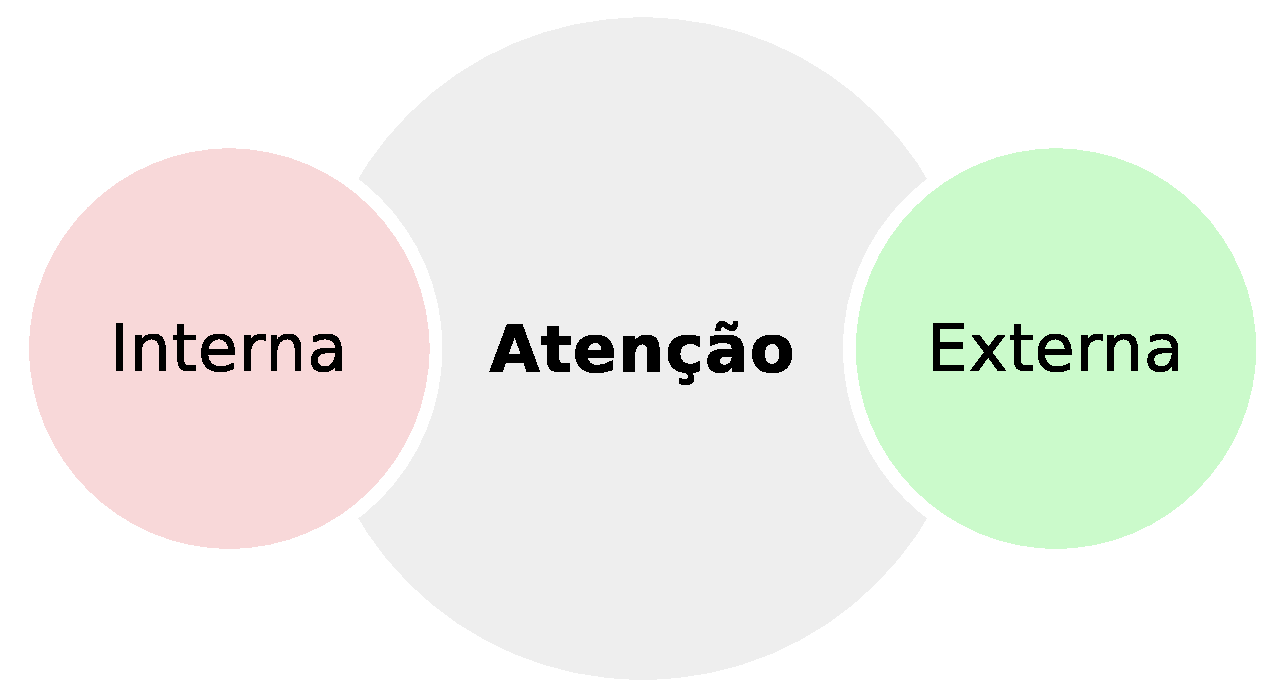
\includegraphics[width=8mm]{attention2.eps}}; }
}

%----------------------------------------------------------------------------------------
% ATTENTION MESSAGE BOX
%----------------------------------------------------------------------------------------
\newtcolorbox{remarcar}
{
  breakable,
  enhanced,
  arc      =1mm,
  colback  =colorsystemdefault!5,
  colframe =colorsystemdefault,
  leftrule =12mm,%
  overlay  ={\node[anchor=north west,outer sep=2pt] at (frame.north west) {\includegraphics[width=8mm]{remarcar.eps}}; }
}


%----------------------------------------------------------------------------------------
% CITANDO MESSAGE BOX
%----------------------------------------------------------------------------------------
% \begin{citando}
%   texto
% \end{citando}
\newtcolorbox{citando}
{
  breakable,
  enhanced,
  colback  = colorlowgray,
  colframe = colorlowgray,
  arc      = 3mm,
  left skip= 0.10 \linewidth,
  width    = 0.90 \linewidth
}

%----------------------------------------------------------------------------------------
% CATALOGRAFICA MESSAGE BOX
%----------------------------------------------------------------------------------------
% \begin{catalografica}
%   texto
% \end{catalografica}
\newtcolorbox{catalografica}
{
  breakable,
  enhanced,
  colback  = colorlowgray,
  colframe = colorlowgray
}


%----------------------------------------------------------------------------------------
% PATROCINIO MESSAGE BOX
%----------------------------------------------------------------------------------------
% \begin{patrocinio}
%   texto
% \end{patrocinio}
\newtcolorbox{patrocinio}
{
  breakable,
  enhanced,
  colback  = colorlowred,
  colframe = colorlowred
}
 % las macros compuestas usadas para la escrita
\definecolor{mydarkolivegreen}{rgb}{0.33, 0.42, 0.18}

\newcommand{\TITULOA}[1]{\noindent\Large\textcolor{mydarkolivegreen}{\textbf{\uppercase{#1}}}\\}
\newcommand{\TITULOB}[1]{\noindent\large\textcolor{mydarkolivegreen}{\textbf{\uppercase{#1}}}\\}

\newcommand{\LINEDATA}[0]{\noindent\rule{\linewidth}{0.4pt}\break}

%\newcommand{\BOXDATA}[0]{\noindent\fbox{\phantom{O}\hspace{\linewidth}}\\}
\newcommand{\BOXDATA}[0]{\noindent\fbox{\makebox[\textwidth]{\phantom{O}}}\\}

\newcommand{\FOOTPAGE}[0]{
	\noindent\includegraphics[width=20px]{youtube.eps}~
	\href{https://www.youtube.com/channel/UCVI2f0odOMVZz4llNbae5Fw}{Dançando e Aprendendo}~
	\hfill\includegraphics[width=20px]{instagram.eps}~
	\href{https://www.instagram.com/dancandoeaprendendo/}{@dancandoeaprendendo}
	
	\noindent\includegraphics[width=20px]{mail.eps}~
	\href{mailto:contato@dancandoeaprendendo.com.br}{contato@dancandoeaprendendo.com.br}~
	\hfill\includegraphics[width=20px]{facebook.eps}~
	\href{https://www.facebook.com/dancandoeaprendendo/}{@dancandoeaprendendo}

}

\newcommand{\showfont}{codifica\c{c}\~ao: \f@encoding{},
  familia: \f@family{},
  serie: \f@series{},
  %shape: \f@shape{},
  e tamanho: \f@size{} pt
}



%----------------------------------------------------------------------------------------

\newcommand{\footwork}[0]{jogo de p\'{e}s}
\newcommand{\Footwork}[0]{Jogo de p\'{e}s}
\newcommand{\Variante}[0]{Variante}
\newcommand{\workboxsize}[0]{1.0\textwidth}
\newcommand{\bodycontrol}[0]{control corporal}
\newcommand{\Bodycontrol}[0]{Control corporal}
\newcommand{\bodyisolation}[0]{dissocia\c{c}\~{a}o corporal}
\newcommand{\Bodyisolation}[0]{Dissocia\c{c}\~{a}o corporal}
\newcommand{\bodyboxsize}[0]{0.75\textwidth}
%%%%%%%%%%%%%%%%%%%%%%%%%%%%%%%%%%%%%%%%%%%%%%%%%%%%%%%%%%%%%%%%%%%%%%%%%%%%%%%%
%%%%%%%%%%%%%%%%%%%%%%%%%%%%%%%%%%%%%%%%%%%%%%%%%%%%%%%%%%%%%%%%%%%%%%%%%%%%%%%%
%%%% Macros para texto
%%%%%%%%%%%%%%%%%%%%%%%%%%%%%%%%%%%%%%%%%%%%%%%%%%%%%%%%%%%%%%%%%%%%%%%%%%%%%%%%

\newcommand{\FALTAPROVA}{\textcolor{red}{[FALTA PROVA!!!]}}
\newcommand{\FALTAREFERENCIA}{\textcolor{red}{[FALTA REFERENCIA!!!]}}
 % My macros
%-----------------------------------------------------------------------------------------
%-----------------------------------------------------------------------------------------

\hyphenation{sam-ba}
\hyphenation{Har-wood}
\hyphenation{mo-vi-men-tar}
\hyphenation{mo-vi-men-tar-nos}
\hyphenation{mo-vi-men-tan-do}

%----------------------------------------------------------------------------------------
% Para a criação do Glossário
%----------------------------------------------------------------------------------------
\makenomenclature



\begin{document}

%----------------------------------------------------------------------------------------
%	TITLE PAGE
%----------------------------------------------------------------------------------------
\newpage

\def \TextAtTopOfPage{\ImprimirEdition}
\def \TextAtBottomOfPage{\imprimiryear}%% {Gerado no dia \today}

\begingroup
\begin{titlepage}
    \newgeometry{left=2.5cm,top=2.5cm,bottom=2.5cm, right=2.5cm}
    %\AddToShipoutPicture*{\put(0,0){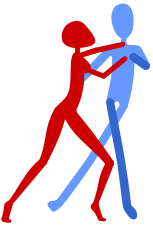
\includegraphics[width=0.49\textwidth]{logo-bw-1}}} % Image background
    \AddToShipoutPicture*{\put(20,0){\includegraphics[width=0.45\textwidth]{cruzado-bonecos-a-gray.eps}}} % Image background
    %\AddToShipoutPictureBG*{\includegraphics[width=\paperwidth,height=\paperheight]{golden-ratio-3}}

\noindent\begin{minipage}{\textwidth}
\parbox[t]{1.0\linewidth}{\centering \fontsize{25pt}{0pt}\selectfont\vspace*{1.4cm}\TextAtTopOfPage\vspace*{0.2cm}}
\end{minipage}
    \begin{minipage}{\textwidth}
        \vspace{4cm}
        \noindent
        \begin{center}
            {\fontsize{60}{70}\selectfont \mytitle\\[0.5\baselineskip]}
            {\fontsize{40}{50}\selectfont \mysubtitle}\\[2\baselineskip]
        \end{center}
        \vspace{35mm}
        \begin{flushright}
            {\fontsize{25pt}{0pt}\selectfont \myauthor}\\[1\baselineskip]
            {\fontsize{25pt}{0pt}\selectfont \imprimirlocal}\\[1\baselineskip]
            {\fontsize{25pt}{0pt}\selectfont \TextAtBottomOfPage}\\[0\baselineskip]
        \end{flushright}
    \end{minipage}
\end{titlepage}
\endgroup


%----------------------------------------------------------------------------------------
%	COPYRIGHT PAGE
%----------------------------------------------------------------------------------------
%\cleardoublepage

\newpage
\thispagestyle{empty}

\noindent Copyright \copyright\ 2020 \myauthor\\ % Copyright notice
\noindent Esta obra é liberada com uma Licença Creative Commons 
Atribuição-NãoComercial-CompartilhaIgual 4.0 Internacional. 
Não é possível usar este arquivo excepto em conformidade com a Licença. 
Pode obter uma copia da Licença em
\url{http://creativecommons.org/licenses/by-nc-sa/4.0/}.\\ % License information

\noindent \textsc{Impresso no Brasil -- ISBN:\imprimirisbn}\\ % Publisher


\textbf{Para investir em pesquisa e colaborar com o projeto:}
\begin{tcolorbox}[breakable,colback=colorlowred,colframe=colorlowred]%%
	\sffamily
	\vspace*{\fill}					% Posição vertical
	\begin{center}					% Minipage Centralizado
	\fbox{\begin{minipage}[c][]{13.5cm}		% Largura

	\small
    Para colaborar com esta pesquisa, você pode comprar uma versão impressa do livro
    desde o seguinte endereço eletrônico:\\
    \ImprimirLinkCompraLivroImpresso ~\\
    Ou pode comprar uma versão digital desde:\\
    \ImprimirLinkCompraLivroDigital ~\\


    \hspace{0.5cm}
    Também pode colaborar com dinheiro em efetivo, desde 20 reais (5 USD), 
    pelos seguintes métodos:
    \begin{itemize}
    \item Método 1
    \item Método 2
    \end{itemize}


    \hspace{0.5cm}
    Se já colaborou com a pesquisa, e se assim o deseja, 
    sintase livre de me mandar um e-mail a \ImprimirEmail, 
    pedindo abordar um novo assunto ou aprofundar em outro.
    Sim seu pedido está dentro das minhas capacidades 
    este será agregado sem falta na seguinte edição do livro.
	\begin{flushright}
    \myauthor ~\\ 
    \end{flushright}

	\end{minipage}}
	\end{center}
\end{tcolorbox}%%



\textbf{Ficha catalográfica}
\begin{tcolorbox}[breakable,colback=colorlowgray,colframe=colorlowgray]%%
	\sffamily
	\vspace*{\fill}					% Posição vertical
	\begin{center}					% Minipage Centralizado
	\fbox{\begin{minipage}[c][5cm]{13.5cm}		% Largura
	\small
	\myauthor.
	%Sobrenome, Nome do autor
	
	\hspace{0.5cm} \mytitle: \mysubtitle   / \myauthor. --
	\imprimirlocal, \imprimiryear.
	
	\hspace{0.5cm} \pageref{LastPage} p. : il. (algumas color.) ; \imprimirsize.\\
	
	%\hspace{0.5cm} \imprimirorientadorRotulo~\imprimirorientador\\
	
	\hspace{0.5cm}
	\parbox[t]{\textwidth}{\imprimirtipotrabalho~--~\imprimireditora,~\imprimirdata.}\\

	\hspace{0.5cm}
	\parbox[t]{\textwidth}{ISBN:\imprimirisbn}\\


	
	\hspace{0.5cm}
		1. Samba de gafieira.
		2. Samba.
		3. Gafieira.
		4. Partitura de movimento.
        5. Musicalidade.
		I. Título 			
	\end{minipage}}
	\end{center}
\end{tcolorbox}%%

~\\

\noindent \textsc{Descarga gratuita da versão eletrônica em \ImprimirLinkDescargaLivro}\\

\noindent \textsc{Publicado por \imprimireditora}\\ % Publisher
\noindent \textit{Primeira impressão , \imprimirdata} % Printing/edition date


%----------------------------------------------------------------------------------------
%	DEDICATORIA
%----------------------------------------------------------------------------------------
\input{\SourceRootPath/pages/dedicatoria} 

%----------------------------------------------------------------------------------------
%	Acknowledgements
%----------------------------------------------------------------------------------------
\cleardoublepage

\begin{center}
\Huge{\textbf{Agradecimentos}}
\end{center}

\null
\vfill
\thispagestyle{empty}

{\normalsize \it \hfill Dou muitas graças a Deus \vspace*{4pt}}


~\\

{\normalsize \it Dou muitas graças a Estevam Lawrence por me 
ajudar a resolver muitas duvidas sobre definições e uso de termos na teoria músical.
\vspace*{4pt}}


{\normalsize \it Dou muitas graças ao Prof. José Henrique de Souza (Henrique Carioca)
por suas aulas de samba no pê, 
e ter-me ensinado dinâmicas para o desenvolvimento da consciência corporal.
\vspace*{4pt}}

\begin{comment}
{\normalsize \it Dou muitas graças a \textcolor{red}{XXXXXXXXXXX} pela 
suas sugestões e revisão  do capitulo \textcolor{red}{XXXXXXXXXXX}.
\vspace*{4pt}}
\end{comment}


 

%----------------------------------------------------------------------------------------
%	PATROCINIO PAGE
%----------------------------------------------------------------------------------------
\input{\SourceRootPath/pages/patrocinio}

%----------------------------------------------------------------------------------------
%	PROLOGO PAGE
%----------------------------------------------------------------------------------------

\cleardoublepage % Forces the first chapter to start on an odd page so it's on the right
\newpage
\thispagestyle{empty}

\chapterimage{chapter_letras.pdf} % Table of contents heading image
\chapter*{Prólogo}
\addcontentsline{toc}{chapter}{Prólogo} %% Sale en la pagina contents
Este livro contem um trabalho de pesquisa e recopilação de informações relativas ao samba de gafieira
e a dança a dois. Entre os assuntos abordados temos: a história do samba como expressão cultural,
os subgêneros musicais do samba e as danças derivadas destas; 
também são presentados alguns conceitos de teoria musical,
musicalidade, teorias sobre o aprendizado, controle e isolamento corporal.  

O livro tem sido criado como uma mensagem do meu eu presente para meu eu futuro,
como uma lembrança permanente sobre conceitos e definições importantes no samba de gafieira e a dança a dois;
porém, ao finalizar esta edição do meu trabalho, 
também tenho a esperança de que esta pesquisa seja útil para as pessoas
que precisem informações básicas ao iniciar seu percorrido no estudo do samba de gafieira.

Fazendo uma analogia com um mapa, 
o livro não representa a marca que indica o final do percorrido 
e sim uma das muitas rotas possíveis para iniciar a avançar na direção desejada;
assim, com o passar dos anos, minha esperança é que seja finalizada a visão iniciada nesta edição do livro.  


%----------------------------------------------------------------------------------------
%	TABLE OF CONTENTS
%----------------------------------------------------------------------------------------
\clearpage
\chapterimage{chapter_letras.pdf} % Table of contents heading image
\pagestyle{fancy} %\pagestyle{empty} % No headers %\pagestyle{fancy} % Print headers again
%\renewcommand{\contentsname}{Indice}
%\phantomsection
%\addcontentsline{toc}{chapter}{Sumário} %% Sale en la pagina part
\tableofcontents % Print the table of contents itself

%----------------------------------------------------------------------------------------
%----------------------------------------------------------------------------------------
%	TABLE OF LISTAS
%----------------------------------------------------------------------------------------
%----------------------------------------------------------------------------------------
\chapterimage{chapter_letras.pdf} % Table of contents heading image
\chapter*{Listas de dados}
\addcontentsline{toc}{chapter}{Listas de dados} %% Sale en la pagina contents

%----------------------------------------------------------------------------------------
%    LISTA DE DEFINICIONES
%----------------------------------------------------------------------------------------
\phantomsection
\addcontentsline{toc}{section}{Lista de definições} %% Sale en la pagina contents
\tcblistof[\section*]{MisDefinicoes}{Lista de definições}
%----------------------------------------------------------------------------------------
%    LISTA DE INFORMACOES
%----------------------------------------------------------------------------------------
\phantomsection
\addcontentsline{toc}{section}{Lista de informações} %% Sale en la pagina contents
\tcblistof[\section*]{MisInformacoes}{Lista de informações}
%----------------------------------------------------------------------------------------
%    LISTA DE ELABORACIONES
%----------------------------------------------------------------------------------------
% temas sueltos que sao elaborado para anhadir riqueza a experiencia de leitura
\phantomsection
\addcontentsline{toc}{section}{Lista de elaborações} %% Sale en la pagina contents
\tcblistof[\section*]{MisElaboraciones}{Lista de elaborações}
%----------------------------------------------------------------------------------------
%    LISTA DE FRASES
%----------------------------------------------------------------------------------------
\phantomsection
\addcontentsline{toc}{section}{Lista de frases} %% Sale en la pagina contents
\tcblistof[\section*]{MisFrases}{Lista de frases}


%----------------------------------------------------------------------------------------
\cleardoublepage % Forces the first chapter to start on an odd page so it's on the right
\pagestyle{fancy} % Print headers again

%----------------------------------------------------------------------------------------
%	PART
%----------------------------------------------------------------------------------------
\part{História}
%%%%%%%%%%%%%%%%%%%%%%%%%%%%%%%%%%%%%%%%%%%%%%%%%%%%%%%%%%%%%%%%%%%%%%%%%%%%%%%%
%% SECTION
%%%%%%%%%%%%%%%%%%%%%%%%%%%%%%%%%%%%%%%%%%%%%%%%%%%%%%%%%%%%%%%%%%%%%%%%%%%%%%%%
\section{\textcolor{green}{Historia do samba}}\index{Historia do samba}
O samba como principal manifestação da cultura brasileira está bem reconhecida no Brasil do seculo XXI;
porem, o caminho da palavra samba, ou da ideia do samba, inicia muito tempo atrás;
pois como mostraremos mais adiante, existiu uma transição entre os termos ``batuque'' e ``samba''.
Nos inícios do seculo XIX
se designava com a palavra ``batuque''  a qualquer reunião de ``pretos'' (em expressões próprias da época) realizando danças entendidas como africanas\footnote{
Porem no Brasil existem registros desta palavra desde o século XVIII \cite[pp. 85]{sandroni2001feitico}. }
\cite[pp. 54]{de4danccas} \cite[pp. 73]{lara2007memoria}.
Um exemplo disto pode ser visto numa carta ao redator do ``Correio Braziliense''  (Londres, ING),
sobre os negócios públicos em Pernambuco,
escrita o dia 3 de dezembro do 1816, e publicada em 1817 \cite[pp. 468]{batuqueBraziliense},
onde se menciona\footnote{\label{footort}A forma da escrita corresponde ao texto original}:
\begin{citando}%%
Quasi dous annos depois, o Ouvidor das Alagoas, que não tinha tido parte neste Drama,
sonhou com outro levante de pretos na sua comarca, 
fundamentado unicamente em um \textbf{batuque} de dança, 
que alguns faziam nas inmmediaçoens de um Engenho de assucar, ...
\end{citando} 
Pelo que se observa, 
a palavra ``batuque'' não se usava para referenciar a uma dança em particular e sim aos festejos dos negros em geral \cite[pp. 85]{sandroni2001feitico}.

\PRLsep{*}

Paralelamente na historia, a palavra samba estava iniciando a ser usada como parte
das expressões nestos festejos populares. 
Isto pode ser visto na ordem do dia do Quartel do Governo das Armas em
Pernambuco, 8 de julho de 1830, publicado no jornal ``Diario de Pernambuco''(PE), 
onde se  relata\footref{footort} \cite[pp. 3]{sambadiariodepernanbuco}:
\begin{citando}%%
Naõ existindo fora da Capital nos diferentes pontos,
onde se achão destacadas as Companhias deste Corpo, 
hum serviço ativo, a que sejão ellas forçadas, 
necessariamente a occiozidade dispora' 
aos mais bem conduzidos a se entreterem nas pescarias de curraes e trapaçoens de coqueiros,
em cujos passatempos sera' recebida com agrado a viola, e o \textbf{samba};
e aos peraltas, cada vez os fara' mais dezenvolvidos na conjugação do verbo surripio.
\end{citando}
Anos posteriores podemos encontrar uma dualidade no uso da palavra samba, 
tanto no sentido de música como de dança; por exemplo, no jornal ``O Capuceiro''(PE),
do dia 3 de fevereiro de 1838, temos uma referencia ao samba como música,
onde ademais se ressalta a beleza da interpretação musical;
o seguinte é um fragmento desse texto\footnote{\label{footort2}A forma da escrita corresponde ao texto original} \cite[pp. 1]{sambaperiodicoocapuceiro}:
\begin{citando}%%
Segue se, que tão perfeita na Cantoria era Catalini, ou a Pasta,
como pai Antonio descantando no seu birimbau; que tanto val huma garatuja da China,
que vinhão nos bules, e bandejas,
como as pinturas de Rafael, de Rubens, ou do Corregio;
que tão agradavel he hum \textbf{samba} d'almocreves, como a Semiramis,
a Gaza-ladra, o Tencredi, \&c. de Rossini, ...
\end{citando}
Também podemos achar outra referencia do samba no sentido musical, no jornal ``Diário do Rio de Janeiro''(RJ),
do dia 19 de abril de 1939, onde se menciona\footref{footort2} \cite[pp. 1]{sambadiariorj1}:
\begin{citando}%%
Em quanto o cortezão, o palaciano, o gamenho, o literato, o magistrado etc., 
espancão melanconias, desvanecem cuidados tomando em ricas bocetas o cheiroso rapé;
o laborioso maluto, a quem furtárão o cavalinho (que é a menina dos seos olhos)
depois de affligir-se, e praguejar em balde arranca do quijeje (bolso na celoura)
o encebado cornimboque, saca lhe com estalo e tapadoura, e chafurdando as ventas em duas,
ou trez pitadas mestras da sua torradinha, esquece-se do cavallo, resigna-se com sua sorte,
e com uma viola nas unhas zangarrêa o \textbf{samba} por uma noite inteira.
\end{citando}
Por outro lado, temos uma referencia ao samba relacionando-o com a dança, no jornal ``O Capuceiro''(PE),
do dia 12 de novembro de 1842\footnote{Só 6 anos apos referenciar o samba como música, 
no mesmo jornal, é usado o mesmo termo agora relacionado com a dança.}, 
onde mencionam\footref{footort2} \cite[pp. 5]{sambaperiodicoocapuceiro2}:
\begin{citando}%%
Aqui pelo nosso mato,\\
Qn'stava então mui tatamba,\\
Não se sabia outra cousa,\\
Senão a \textbf{dansa do samba}.
\end{citando}
Neste ultimo texto vemos que ainda se diz a \textbf{dança do samba} e não dançar o samba,
mas é possível observar como o termo vai se fusionando com a dança.
Seguindo esta linha de pensamento, 
podemos ver outro exemplo no Jornal ``O Guaycuru''(BA), do dia 26 de maio de 1846,
onde podemos ler o seguinte texto\footref{footort2} \cite[pp. 2]{sambaperiodicooguaycuru}:
\begin{citando}%%
Todavia o famigerado Salles, sem respeito algum aos institutos de sua ordem, 
foi-se pòr na Cachoeira a divertir talvez \textbf{dançando o samba}...
Que bello exemplar da vida religiosa!?
\end{citando}
Como tem sido visto, 
para esta data já se podia ver como as pessoas entendiam o samba como uma dança.
Porem, não terá que se esperar muito pra achar referencias mostrando ao samba
como uma expressão cultural em si mesma, 
uma declaração deste tipo pode ser achada no jornal ``O Cosmorama na Bahia'' (BA), 
no dia 15 de dezembro de 1849, onde menciona\footref{footort2} \cite[pp. 2]{sambaperiodicoocosmorama}:
\begin{citando}%%
Cousa já muito antiga para engordar os patinhos. 
Para o espectaculo seguinte haverá um \textbf{SAMBA} á moda da Bahia, 
em que entram os negreiros todos.
\end{citando}

\PRLsep{*}
Retomando o tema do batuque

\PRLsep{*}


Assim, como mostrado anteriormente e resumindo as ideias, 
na literatura do Brasil já temos referencias da palavra ``samba'' desde o ano de 1830; 
porem como menciona Sandroni C. no seu livro ``Feitiço decente: transformações do samba no Rio de Janeiro'', 
falando especificamente do Rio de Janeiro, 
a palavra samba foi pouco conhecida ate o último quartel do século XIX \cite[pp. 86]{sandroni2001feitico};
este dado cobrará importância quando o termo seja relacionado com as gafieiras.
Por outro lado, a palavra  ``batuque'' usada para designar festejos populares com danças, foi muito recorrente ate inícios do seculo XX, 
onde a palavra ``samba'' virou mais popular para descrever estas atividades \cite[pp. 85]{sandroni2001feitico} \cite[pp. 47]{diniz2008almanaque}; 
a Figura \ref{fig:sambacrono} descreve o uso destas palavras ao longo do tempo.
\begin{figure}[h]
  \centering
    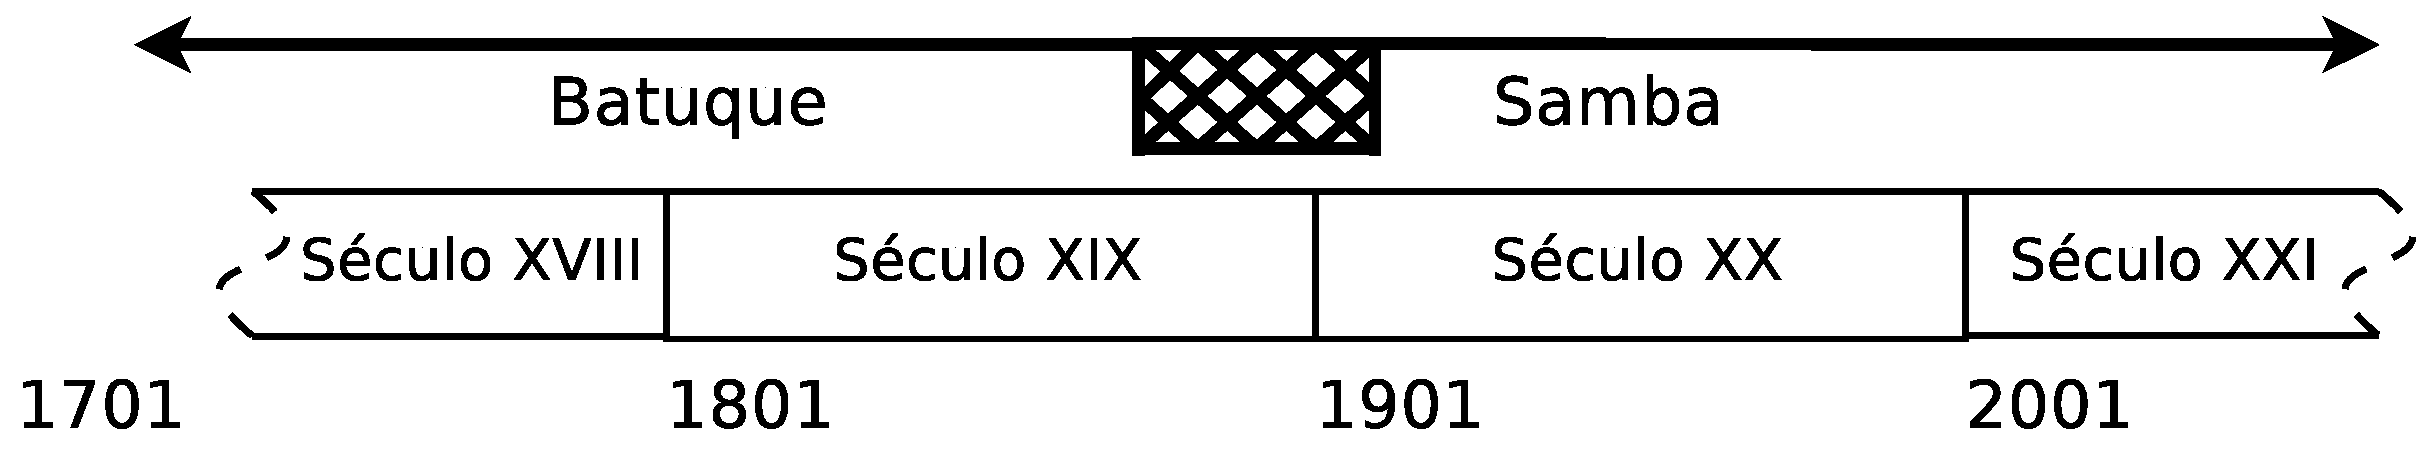
\includegraphics[width=0.85\textwidth]{chapters/cap-historia/samba-crono.eps}
  \caption{Cronologia da designação geral dos festejos de pessoas, de raça negra, no Brasil.}
  \label{fig:sambacrono}
\end{figure}


Entre as explicações da origem da palavra ``samba'', 
a mais conhecida, é a que promove que esta vem do idioma quimbundo, 
sendo derivado da palavra ``semba''  que significa umbigada \cite[pp. 47]{diniz2008almanaque} \cite[pp. 50]{da2015historia}.
Uma referencia muito conhecida deste vinculo é a descrita no livro ``O negro e o garimpo em Minas Gerais''
de Mata Machado Filho, onde ele comenta que ``os negros corrigem para semba se 
alguém lhes fala em samba'' \cite[pp. 85]{sandroni2001feitico}. Assim se vê que existe
desde antanho uma relação entre as palavras, 
samba, semba e umbigada.

\begin{comment}
Entre as danças "profanas" \cite[pp. 85]{sandroni2001feitico} afro-brasileiras o gesto da umbigada é um elemento muito caraterístico,
de modo que em 1961 Edson Carneiro definiu e englobou as danças que realizam este 
gesto como ``samba-de-umbigada'' . Assim tradições 
musicais como o samba de roda, o jongo, o lundu, o coco, o calango e o cateretê, 
seguindo Edson são englobadas com  ``samba-de-umbigada'' \cite[pp. 85]{sandroni2001feitico}.
\end{comment}


%%%%%%%%%%%%%%%%%%%%%%%%%%%%%%%%%%%%%%%%%%%%%%%%%%%%%%%%%%%%%%%%%%%%%%%%%%%%%%%%
%% Capitulo
%%%%%%%%%%%%%%%%%%%%%%%%%%%%%%%%%%%%%%%%%%%%%%%%%%%%%%%%%%%%%%%%%%%%%%%%%%%%%%%%
\chapterimage{chapter_head_2.pdf} % Chapter heading image

\chapter{Historia das gafieiras}
\index{Historia das gafieiras}

%%%%%%%%%%%%%%%%%%%%%%%%%%%%%%%%%%%%%%%%%%%%%%%%%%%%%%%%%%%%%%%%%%%%%%%%%%%%%%%%
\section{Gafieira}
\label{def:Gafieira}
\index{Gafieira}
Atualmente o termo gafieira indica um baile de clube particular, com entrada paga e frequência livre. 

\begin{itemize}
\item \textbf{1979 em adiante:} Se entende que as gafieiras são locais de lazer 
e dança onde existe bom comportamento e muita compostura,
em perfeita integração racial; de modo que, 
a gafieira é sinônimo de baile em salão espaçoso como boa música orquestral \cite[pp. 10-11]{respeitojournalbrasil1}.

\item \textbf{1932 ate antes de 1979:} O termo gafieira foi associado a lugares de baixa ralé, onde 
se aconteciam frequentemente delitos e trágicos acontecimentos \cite[pp. 11]{gafieirajournalbrasil1} \cite[pp. 12]{gafieirajournaloradical1} \cite[pp. 10-11]{respeitojournalbrasil1}.

\item \textbf{1932:} popularização do termo gafieira, apos o
incidente entre o jornalista Romeu Arêde (Picareta) e o empresario e fiscal de salão Júlio Simões,
que provocou que  Picareta publica-se uma matéria apontando 
ao clube de Júlio como uma gafieira \cite[pp. 3 - cad. 3]{juliosimoes} 
\cite[pp. 21]{efege1974maxixe} \cite[pp. 78]{coutinho2006cronistas};
pelo que este último decidiu apelidar seu exitoso ``Elite clube'' como gafieira;
espalhando-se rapidamente esta denominação a outros clubes similares. 
Assim, o termo queda vinculado a clubes de dança da classe média,
onde eram aceitos todas as pessoas sem nenhum tipo de preconceito racial, 
prévio pago da entrada \cite[pp. 6 - cad. B]{entrevistajuliojournalbrasil1}.


\item \textbf{1917 ate 1932:} 
Inícios do uso do termo gafieira, indicando bailes populares \cite[pp. 29]{instituto1987revista} de entrada paga
ou bailes criados por motivo do carnaval; sendo que, as referencias bibliográficas
achadas são nas semanas próximas ao carnaval \cite[pp. 4]{oldgafieira1} 
\cite[pp. 7]{oldgafieira2} \cite[pp. 4]{oldgafieira3} \cite[pp. 5]{oldgafieira4},
o que mostra a notoriedade que adquiriam esses eventos, ou locais, nessas datas.
\end{itemize}

%%%%%%%%%%%%%%%%%%%%%%%%%%%%%%%%%%%%%%%%%%%%%%%%%%%%%%%%%%%%%%%%%%%%%%%%%%%%%%%%
\section{Cronologia das gafieiras}


%%%%%%%%%%%%%%%%%%%%%%%%%%%%%%%%%%%%
%\PRLsep{Bailes na década de 1800}

Seguindo o jornalista Agostinho Seixas,
entre os anos de 1847 e 1848, na Cidade Velha, no Rio de Janeiro,
já existiam  bailes e clubes recreativos, 
que hoje denominaríamos como \textbf{gafieiras} \cite[pp. 11]{respeitojournalbrasil1}.
Seixas achou como primeira referencia na suas pesquisas, que entre essas datas,
Dona Francisca Pacheco da Silva, fazia um requerimento 
à ``Excelentíssima Câmara'' (que foi concedido) para a autorização 
da sua sala de bailes, na Rua da Alfândega, 327 \cite[pp. 11]{respeitojournalbrasil1} \cite[pp. 71]{perna2002samba};
este requerimento foi catalogado como sala de danças, 
com a característica de ter entrada paga.
Seguindo o fiscal que acompanhava o requerimento,
ele não achava artigo que regulamentasse esse tipo de local 
de diversão ou dança; lembremos que nessa época
o padrão era ter clubes fechados que tinham um determinado número de sócios \cite[pp. 11,12]{respeitojournalbrasil1}.



%%%%%%%%%%%%%%%%%%%%%%%%%%%%%%%%%%%%
\PRLsep{Bailes na década de 1900}


Para inícios do século XX, podiam ser achadas varias associações para negros e mestiços, 
com distintas  finalidades, como: sociedades beneficentes, literárias, dramáticas, esportivas 
e as ``sociedades dançantes e recreativas'' abertas a um público geral
\cite[pp. 154-155]{neres1999negro} \cite[pp. 71]{de2008bexiga}.
Estas associações geralmente não tinham local próprio, 
e tinham que alugar espaços que terminavam sendo salões de velhos sobrados
ou similares \cite[pp. 154-155]{neres1999negro} \cite[pp. 49]{diniz2003almanaque}.
Entre as organizações sociais recreativas mais comuns da época tínhamos, 
os cordões\footnote{Os cordões eram grupos festivos de dança e música, 
com pessoas mascaradas com figurinos de reis, de
bichos, de pajens, de guarda, etc., tocando instrumentos africanos \cite[pp. 23-24]{fernandes2001escolas}},
os ranchos\footnote{Quando os cordões desapareceram estes se transformam em ranchos (depois de 1908), 
agregaram instrumentos de corda e metais, e inciou a ser tocado a marcha-rancho,
os ranchos eram cordoes mais civilizados \cite[pp. 24]{fernandes2001escolas}} 
e os zé-pereiras\footnote{ Uma sociedade recreativa do ``Ze-pereira''
é uma sociedade dedicada a dança carnavalesca \cite[pp. 10]{simoesjournalbrasil1}} 
\cite[pp. 10]{simoesjournalbrasil1}.


Uma destas sociedades de dança do inícios do seculo XX, que agora definiríamos como gafieira, 
foi a ``Sociedade de Danças Clovis Invencivel''\footnote{Em algumas versões 
``Clovis Invencivel'' é referenciado como ``Clowns Invencíveis'' \cite[pp. 3 - cad. 3]{juliosimoes} ou 
``Clovis Invencíveis'' \cite[pp. 10]{simoesjournalbrasil1}}, 
esta foi fundada no Rio de Janeiro em 1906, 
na qual eram populares concursos de valsa, polca ou quadrilha \cite[pp. 6 - cad. B]{entrevistajuliojournalbrasil1}.
O dono da ideia da criação destes concursos foi um muito jovem e fiscal do salão, Júlio Simões,
que a seus 16 anos pensou numa sociedade de dança diferente dos da época,
que se dedicavam a ``bater bumbo'' (bailes carnavalescos ou de zé-pereira), 
a uma dedicada a ``arrasta-pés'' (bailes de salão) 
\cite[pp. 6 - cad. B]{entrevistajuliojournalbrasil1} \cite[pp. 3 - cad. 3]{juliosimoes} \cite[pp. 10]{simoesjournalbrasil1}.

Com o surgir dos lugares de baile, em 1915 \cite[pp. 1 - cad. B]{gafieira2000reis},  
Júlio Simões, foi chamado pelos sócios\footnote{Os 
sócios fundadores da ``Kanaga do Japão'' são José Constantino da Silva 
e José de Paiva Brito \cite[pp. 1 - cad. B]{gafieira2000reis}} da ``Kanaga do Japão'' para dirigir seu novo clube,
lugar de grande tradição no Rio de Janeiro, e muito popular na época,
no qual o conjunto encarregado de animar o local era chefado por Sinhô e Bulhões de Carvalho,
que receberam o título popular de ``reis da valsa'',
com torneios de dança que duravam ate 55 
minutos dançando uma valsa rápida \cite[pp. 3 - cad. 3]{juliosimoes} \cite[pp. 1 - cad. B]{gafieira2000reis} \cite[pp. 6 - cad. B]{entrevistajuliojournalbrasil1}.
Nas festas comandadas por Júlio, era comum ver dançar samba, polca, 
valsa e quadrilha, que ele mesmo marcava no salão \cite[pp. 1 - cad. B]{gafieira2000reis}. 


Para o ano 1930, estas sociedades dançantes tinham ganhado muita popularidade. 
Assim, apos a morte de um socio e o fechamento da ``Kananga do Japão'' 
em 1929 \cite[pp. 3 - cad. 3]{juliosimoes}  \cite[pp. 11]{eliteinaugura} \cite[pp. 1 - cad. B]{gafieira2000reis}, 
Júlio Simões procura a Heitor Persegani e  Hilário Jovino, 
e decidem fundar o local de danças chamado ``Elite club'' \cite[pp. 11]{eliteinaugura} \cite[pp. 13]{respeitojournalbrasil1},
agora chamado ``Elite clube'' \cite[pp. 3 - cad. 3]{juliosimoes},
na Rua Frei Caneca n. 4 - Centro, Rio de Janeiro - RJ;
sendo o 17 de julho de 1930 seu baile inaugural 
\cite[pp. 11]{eliteinaugura} \cite[pp. 3 - cad. 3]{juliosimoes} \cite[pp. 10]{simoesjournalbrasil1}.

Uma descrição de uma destas sociedades dançantes, anterior a 1931, pode ser vista no livro "O cabrocha"; 
escrita  por Jota Efegê em 1931; 
sobre a ``Sociedade Recreativa Familiar Bohemios de Botafogo'' \cite[pp. 24-26]{jotaefege},
a continuação é mostrado um extracto desse texto:
\begin{citando}%%
O salão, comquanto não fosse de grandes dimensões, era
de um tamanho regular, confinando com uma pequena saleta
onde tambem se dansava; estava bem affluido. Numa
heterogeneidade foliã, via-se desde a crioulinha blasée, sem
elegancia, desalinhada, á mulatinha pernostica de faces
avermelhadas por um carmin berrante, cabello engommado e
subjugado por travessas e grampos, num á la garçonne
forçado, mas exigido pela moda. Em meio dessas "cabrochas"
e "roxinhas", viam-se algumas moças brancas de apparencia
sobria. São as meninas que não podem fazer um vestido de
seda ou calçar sapatos de setim, para se apresentarem no
Fluminense ou no Flamengo e que nestes clubes se divertem,
ficando em evidencia por serem brancas.  %~\\
(Jota Efegê)
\end{citando}

%%%%%%%%%%%%%%%%%%%%%%%%%%%%%%%%%%%%
\PRLsep{Inícios do uso do termo gafieira}

Fazendo uma pesquisa na ``Biblioteca Digital da Fundação Biblioteca Nacional''
podemos achar referencias ao termo \textbf{gafieira} desde 1917\footnote{Mesmo 
ano em que foi lançado o samba ``Pelo telefone'', sendo um exito total no carnaval desse ano.}.


A primeira referencia pode ser vista no jornal ``O Imparcial'' (RJ),
do dia 17 de janeiro de 1917, como o título ``Batalha de confetti'',
no qual se anuncia que na rua Guimarães se terá uma grandiosa batalha,
organizada pelo ``bloco dos pesados'', conformado por \cite[pp. 4]{oldgafieira1} \cite[pp. 629]{spielmann2016reflexoes}:
\begin{citando}
Lourenço dos Santos (Lord Sorvete),\\
Antonio dos Santos (Lord Massa),\\
Antonio Lima (Lord Repinica),\\
Raul Dantas (Lord Ronqueira),\\
Almeidinha (Lord Prrrrr...!),\\
Arlindo dos Santos (\textbf{Lord Gafieira}),\\
Joaquim Mello (Lord Frango d'Agua),\\
Juvenal Branco (Lord Pé Pequeno),\\
Eudoxio dos Santos (Lord Garganta) e\\
Jorge Vença (Lord Come Bola).
\end{citando}
Pelo contexto do anuncio, e pela semelhança com os outros apelidos, 
pode-se perceber que o termo \textbf{gafieira} tem um significado alegre,
cotidiano ou extravagante, mas é difícil extrair alguma outra conclusão.

A seguinte referencia aparece um ano depois, no mesmo jornal,
no dia 8 de fevereiro de 1918, como o título ``Grande batalha de confetti'',
na qual se anuncia que a batalha é organizada pelo ``bloco da rapaziada'',
do ``\textbf{Club da Gafieira}'', a qual também terá a participação 
da \textbf{orquestra do ``Gafieira''} que tocará adoráveis tangos;
e se finaliza falando que  \cite[pp. 7]{oldgafieira2} \cite[pp. 629]{spielmann2016reflexoes}:
\begin{citando}
Serão distribuídos brindes áquelles que mais se têm distinguido nos bailes do valoroso ``\textbf{Gafieira}''.
\end{citando}
Nesta referencia, já podemos observar que a palavra gafieira é relativa à celebrações do carnaval, 
e a lugares ou eventos de bailes,
nos quais, por exemplo, se dançam tangos; 
pelo que a palavra \textbf{gafieira} é usada no nome da orquestra,
e no apelido de um integrante, o valoroso \textbf{Gafieira}.

Um ano depois na ``Gazeta de Noticias'' (RJ),
no dia 3 de março de 1919, com o título ``Club dos carnavalescos do Andarahy'' e subtitulo ``1ra Critica - A Gafieira'',
se anuncia que a ``Banda de clarins'' e a ``Banda de música'',
tocarão uma espirituosa ``charge'' aos bailes de clubs de mil réis por cabeça, 
na qual era  usada a seguinte letra \cite[pp. 5]{oldgafieira3} \cite[pp. 629]{spielmann2016reflexoes}:
\begin{citando}
Cinco tostão vale a varsa!\\
Grita o fiscal do salão:\\
Tirem as dama depressa,\\
Não perquem a casião!\\ ~\\
Sapeca o piston com força,\\
Requebra mais, já se vê!\\
Que depois da contradança,\\
A dama vai p'r'o bufê.\\ ~\\
Paga a entrada e não estrilla!!\\
Que isto aqui é uma deliça!\\
Se porte bem, seu varsista!\\
Cuidadinho e'n a poliça!...
\end{citando}
Nesta última referencia já podemos ver claramente o sentido do termo gafieira,
identificando a um lugar de dança, em especifico a esses lugares com entrada paga a mil réis por cabeça.
Para ter uma ideia de se este preço é pouco ou muito, podemos compará-lo com o 
preço do jornal em que foi publicado o texto, sendo este de 100 RS \cite[pp. 1]{oldgafieira3};
ou também por essas épocas, 
quando a entrada custava 2 mil réis o preço de uma cerveja  era  de 800 réis \cite[pp. 1 - cad. B]{gafieira2000reis}.
Outro dado interessante é o uso do termo ``fiscal de salão'', 
figura de autoridade que já estava presente 
nas sociedades dançantes do seculo XX, como por exemplo na 
``Sociedade de Danças Clovis Invencivel'' em 1906, pelo que queda claro
a que lugares se refere o termo gafieira.


Podemos ver outra noticia relativa as gafieiras, no dia 19 de janeiro de 1920, 
no jornal ``A Razão'' (RJ), no qual se
publica uma reportagem com o título 
``Charivari num club suburbano - Fechado pela policia'',
se referindo ao clube ``Fenianos de Cascadura'',
que seguindo o descrito, este clube era 
ponto de reunião de gente desclassificada, 
que realizava seus bailes os sábados e domingos,
cobrando na entrada $1\$100$ por cabeça.
O seguinte texto é uma porção daquela reportagem \cite[pp. 4]{oldgafieira4} \cite[pp. 629]{spielmann2016reflexoes}:
\begin{citando}
A policia local, que é a do $20^o$ districto,
já estava farta do trabalho que o club 
constantemente lhe dava e de receber reclamações 
dos moradores visinhos.\\
Deliberou então o delegado, dr. Coelho
Gomes, fechar o club, mais conhecido por 
``\textbf{Gafieira}'', na primeira occasião que `e apresentasse.\\
Ante-hontem, sabbado, á noite, o club 
deu o acostumado ``baile'' e ás 5 horas da 
madrugada houve, ali um ``charivari'' medonho,
que poz o largo de cascadura em polvorosa. 
\end{citando}
O termo charivari se usa para indicar música discordante, 
confusão, motim, tumulto, barafunda \cite[pp. 53]{almeida1996dicionario}, etc.
Assim, podemos ver como o termo gafieira, 
estava relacionado a clubes de dança com entrada paga,
e que era frequentado por pessoas de poucos recursos econômicos. 
Também é interessante ressaltar que as referencias achadas correspondem,
a datas próximas ao carnaval, o que mostra o vinculo ou o maior interesse 
destes locais nestas datas. 

Ainda podem ser achadas outras referencias ao termo \textbf{gafieira} na década de 1920,
nelas podemos destacar apelidos usados por professores de dança,
ou referencias de musicas com letras indicando que gafieiras 
são frequentadas por crioulas e/ou criadas.


%%%%%%%%%%%%%%%%%%%%%%%%%%%%%%%%%%%%
\PRLsep{Popularização do termo gafieira}

Seguindo o jornalista e cronista, Jota Efegê, %%Júlio Simões e o historiador,
o termo ``gafieira'' foi criado pelo cronista carnavalesco, 
Romeu Arêde\footnote{Em algumas versões está  referenciado como Romeu Aredo \cite[pp. 188]{raca1999}.}, 
também conhecido como ``Picareta'' \cite[pp. 29]{instituto1987revista}\cite[pp. 3 - cad. 3]{juliosimoes} 
\cite[pp. 21]{efege1974maxixe} \cite[pp. 78]{coutinho2006cronistas}, 
colunista da seção recreativa do ``Jornal do Brasil'' desde 1930 ate 1941
e anteriormente do vespertino ``Vanguarda'' (1922-1930) \cite[pp. 58-59]{efege1982figuras} 
\cite[pp. 6 - cad. B]{entrevistajuliojournalbrasil1};
porém não é indicada, por Jota Efegê, referencia nenhuma sobre a data de criação.
Efegê indica que o termo ``gafieira'', possivelmente deriva de 
``cabroeira''\footnote{Cabroeira: Malta de indivíduos chamados cabras, 
de capangas assalariados para assassinar ou para fazer o mal \cite{diciocabroeira}.} 
ou ``gaforinha'' \cite[pp. 3 - cad. 3]{juliosimoes}.
Por outro lado, Júlio Simões, socio e administrador do ``'Elite club', 
afirma\footnote{Seguindo a ``Revista do Instituto Histórico e Geográfico do Rio de Janeiro'' (1987),
Jota Efegê afirma que foi Romeu Arêde quem atrelou o termo gafieira aos clubes de dança no incidente no ``Elite clube''.} 
que o jornalista Romeu Arêde tinha a costume de entrar, 
comer, beber, dançar e não pagar \cite[pp.13 ]{respeitojournalbrasil1},
e que quando ele impediu ao boêmio jornalista e seus acompanhantes (5 ou 6) o ingresso no ``Elite'', 
porque a entender de Júlio o jornalista estava meio ``alegre'' devido a uns tragos a mais;
 Júlio indicou: ``Aqui tem ordem'' 
\cite[pp.13 ]{respeitojournalbrasil1} \cite[pp. 6]{gafieiraaredeout2} \cite[pp. 3 - Encontro]{gafieiraaredeout1},
indicando que só podiam passar com entrada franca ele mais uma dama ou um amigo;
o cronista então reagiu indicando a seus acompanhantes a se retirarem, 
exclamando \cite[pp. 29]{instituto1987revista} \cite[pp. 6 - Tribuna Bis]{gafieiraaredeout3}: 
\begin{citando}
Vamos embora! Isto aqui é uma gafieira!
\end{citando}
Outras referencias apontam que o que falou foi \cite[pp. 6]{gafieiraaredeout2} \cite[pp. 3 - Encontro]{gafieiraaredeout1}:
\begin{citando}
O que eu vou fazer nessa gafieira?
\end{citando}
Ao dia seguinte Picareta escreveria na sua coluna no Jornal do Brasil \cite[pp. 188]{raca1999}:
\begin{citando}
Aquele é um lugar da ralé, onde se cometem gafes em fieiras
\end{citando}
Varias referencias apontam que este incidente aconteceu em 1932 \cite[pp. 3 - Encontro]{gafieiraaredeout1} \cite[pp. 188]{raca1999}, 
porém não se menciona o dia exato. 




Assim, em qualquer das explicações da formação da palavra gafieira,
seja por ``cabroeira''+``gaforinha'' ou ``gafes''+``fieira'',
esta era uma denominação pejorativa para indicar a um local (``cabroeira'' ou ``gafes'').
É importante lembrar que o termo \textbf{gafieira}, já existia desde antes do 
incidente entre Júlio Simões e Romeu Arêde no ``Elite club'', 
especificamente se tem constância do uso desde 1917 \cite[pp. 4]{oldgafieira1},
pelo que para a data da apertura do ``Elite club'' em 1930,
este termo já estava no consciente de algumas pessoas, porém não estava popularizado;
pelo que se deduz que Romeu Arêde, por conta do incidente no ``Elite club'', 
atuou como catalisador para a popularização do termo gafieira.
%mas isto não descarta a informação de Jota Efegê que indica que foi Arêde quem criou o termo,
%pois  Efegê não menciona uma data especifica.

Júlio simões apos o incidente no ``Elite club'', 
decide devolver a piada e apelidar seu local como 
``Gafieira'', conservando o nome de clube, 
mas transformando-se na pratica em ``Gafieira Elite'' \cite[pp. 79]{moura1995tia} \cite[pp. 6 - Tribuna Bis]{gafieiraaredeout3}.
Por este incidente e suas repercussões, 
muitos autores consideram a ``Elite'' como a primeira gafieira do Brasil \cite{cabral2016elisete} \cite[pp. 84]{cabral1996escolas}.
Consequentemente, e em palavras de Jota Efegê, 
se considera a Júlio Simões como o criador das gafieiras \cite[pp. 3 - cad. 3]{juliosimoes}.

Nesse ponto da historia, 
o nome ``gafieira'' cobrou muita relevância e locais de dança apelidados como gafieiras surgiram no Rio de Janeiro;
depois de tudo, já existissem lugares com estas caraterísticas desde inícios do século XX \cite[pp. 49]{diniz2003almanaque}.
Os salões foram criadas a semelhança dos bailes de salão da classe média ou alta \cite[pp. 78]{coutinho2006cronistas}; 
porém, no caso das gafieiras, estas eram abertas ao público prévio pago da entrada.
A Figura \ref{fig:gafieiracrono} mostra a cronologia do uso da palavra gafieira para os salões de dança no Rio de Janeiro.
\begin{figure}[h]
  \centering
    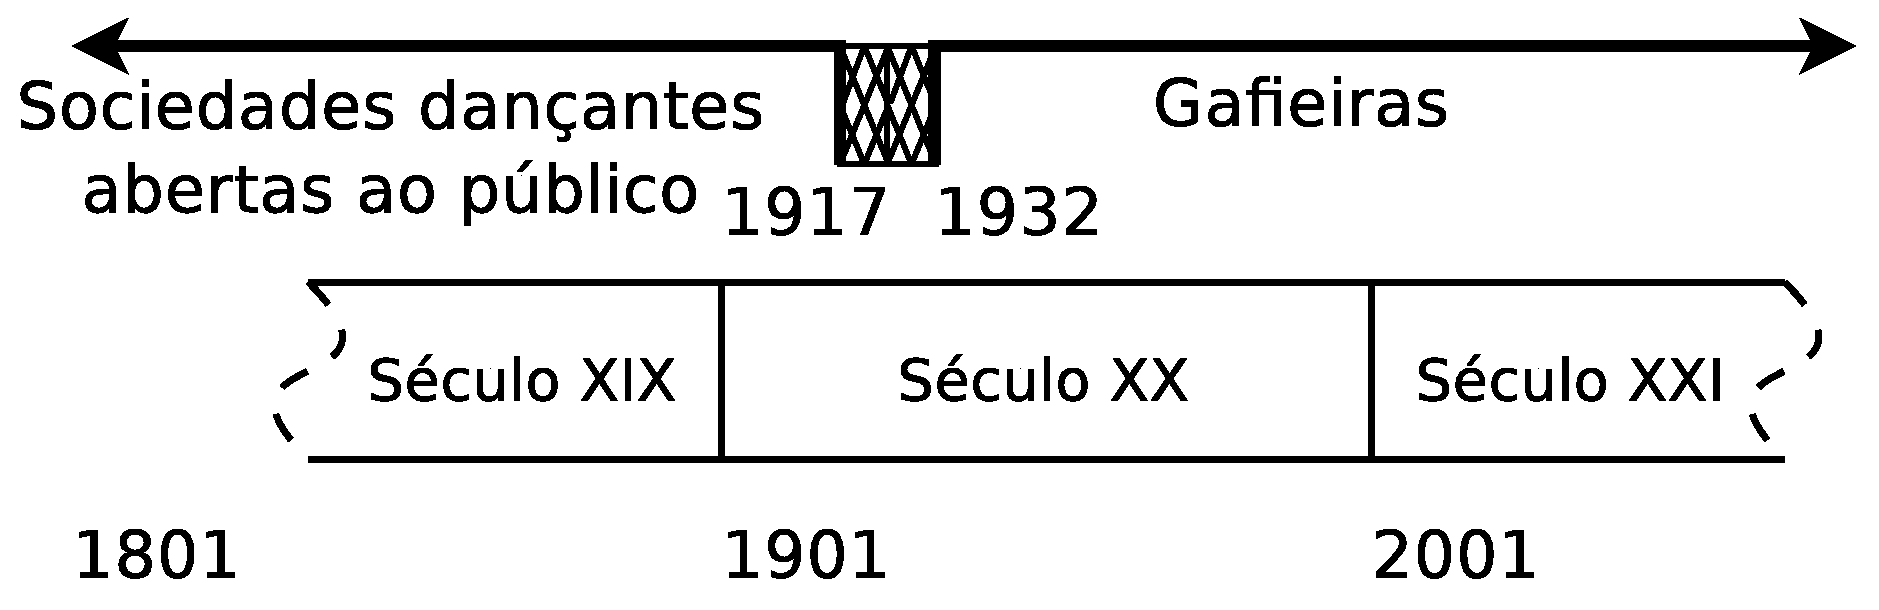
\includegraphics[width=1.0\textwidth]{chapters/cap-historia-gafieiras/gafieira-crono.eps}
  \caption{Cronologia da designação de gafieira para os salões de dança no Rio de Janeiro.}
  \label{fig:gafieiracrono}
\end{figure}

\PRLsep{Delitos vinculados com as gafieiras}

Podemos achar uma referencia ao termo gafieira no jornal ``O Radical'' (RJ),
no dia 8 de setembro de 1932 \cite[pp. 12]{gafieirajournaloradical1},
com o titular:
\begin{citando}%%
A sahida do baile: Por causa de Aracy, o estivador foi ferido á baia.\\
... Na rua Domingo Lopes, n. 243, em Madureira, está situado o club de dança Ideal, 
conhecido pelos moradores locaes por ``Gafieira''.
\end{citando} 
Ao dia seguinte, 9 de setembro de 1932, o jornal ``A Batalha'' (RJ), 
usava também a palavra ``gafieira'' para se referir ao mesmo incidente \cite[pp. 8]{gafieirajournalabatalha1}.

O ``Jornal do Brasil'', o dia 9 de janeiro de 1934, 
usa também a palavra gafieira \cite[pp. 11]{gafieirajournalbrasil1}, com o titular:
\begin{citando}%%
À porta de uma ``gafieira''.
Ainda o conflito da madrugada de domingo no largo de Madureira.
Faleceu um dos soldados no Hospital da Policia Militar. 
Ha no largo de Madureira uma sociedade dansante, mais conhecida por ``gafieira'', 
com entradas retribuidas, ondem de quando em quando, se registram conflitos, 
alguns de graves consequências...
\end{citando} 
Como é visto nas refecerias antes mostradas, e guardando semelhança com outras coincidências
posteriores que podem ser achadas na ``Biblioteca Digital da Fundação Biblioteca Nacional''; 
o termo gafieira, estava associado a lugares considerados perigosos;
isto propiciado pelo aumento do número de locais que se atribuíam este nome, junto com 
a diversidade e cultura  do seu público e administradores.
Porém, este não seria o padrão pelo qual se regiam todas as gafieiras, 
e certamente a conotação mais perigosa ou pejorativa iria mudando no tempo. 

\PRLsep{A gafieira limpa seu nome}

Por exemplo, sobre o Elite Club,  nos sabemos que funcionava as quintas, sábados e domingos,
e existia um fiscal no salão (o velho Russo)\cite[pp. 37]{gafieirajournalmanchete}, 
que fazia cumprir estritamente as normas de bom-tom, comportamento social e respeito ao ambiente, como todo clube familiar precisa ter \cite[pp. 12]{respeitojournalbrasil1}; de modo que, 
não eram admitidas damas que não estivessem de sapatos de salto alto \cite[pp. 37]{gafieirajournalmanchete};
homens embriagados não entravam e o traje indispensável era o paletó e gravata, 
ou no mínimo camisa fechada \cite[pp. 6 - cad. B]{entrevistajuliojournalbrasil1}.
O cavaleiro não podia abraçar a dama nem sentado na cadeira \cite[pp. 6 - cad. B]{entrevistajuliojournalbrasil1},
né dançar de rosto colado, ou por a mão nas costas da dama sem usar lenço \cite[pp. 10]{simoesjournalbrasil1}, 
quem fiscalizava, na porta, era um preto velho tratado por todos de ``titio''  \cite[pp. 37]{gafieirajournalmanchete}.
Se alguma regra não era cumprida, o seu Júlio, jogava a qualquer um para fora \cite[pp. 6 - cad. B]{entrevistajuliojournalbrasil1}.
Nos bailes dedicados ao padroeiro, todo 20 de janeiro, era obrigatório vestir de branco,
já seja no traje ou no vestido, incluindo sapatos e camisas \cite[pp. 37]{gafieirajournalmanchete}.
Tão grande era o censo de ordem dos frequentadores do Elite Club, 
que lhe era permitido operar estando a menos de 80 metros de um hospital,
sendo que nessa época existia a Lei n. 1.590 de 1924, 
seguindo a qual nenhuma casa de diversões podia estar a menos de 200 m de estabelecimentos hospitalares,
Ate o próprio Delegado Dulcídio Gonçalves, da Delegacia de Costumes,
dispensava-se de mandar policiar o Elite.
``À casa do Júlio não precisa de policiamento'', dizia o Delegado Dulcídio
\cite[pp. 5]{simoesjournalalutademocratica1}.


Assim, ao transcorrer dos anos, essa visão popular mais obscura da palavra gafieira foi mudando;
pelo qual o jornalista Francisco Duarte, o dia 12 de agosto de 1979,
escreve no Jornal do Brasil (RJ) sobre este assunto com o título:
``Gafieira - Tratado geral do ambiente que exige respeito'' \cite[pp. 10]{respeitojournalbrasil1}:
\begin{citando}%%
... o verbete Gafieira com o significado de baile reles, arrasta-pé, baile popular de baixa categoria.
No passado, encarada com má vontade pelos puristas do léxico e pela burguesia republicana dançante,
pode ter sido assim. Mas em 1979 -- e cabe aos dicionaristas verificar in loco --
gafieira é baile de clube particular, com entrada paga e freqüência livre, 
local de lazer e dança onde existe bom comportamento e muita compostura,
em perfeita integração racial.\\
(Francisco Duarte)
\end{citando}
Além da afirmação anterior, 
o jornalista explica como a ``Delegacia de Diversões Públicas'' classifica as casas de dança;
assim temos: 
\begin{itemize}
\item ``boates'', que são bar restaurantes com pista de dança e palco para show;
\item ``cabarés'', onde se bebe, come, dança e se tem espetáculos de variedades;
\item ``dancings'' onde se dança mediante pagamento em cartões e picotes; e 
\item ``inferninhos'' que são boates de baixa categoria, 
frequentados por pessoas de vida irregular e onde se toca música barulhenta.
\end{itemize} 
Em palavras de Duarte, ``Gafieiras são sinônimos de baile em salão espaçoso como boa música orquestral'' \cite[pp. 11]{respeitojournalbrasil1}.




%%%%%%%%%%%%%%%%%%%%%%%%%%%%%%%%%%%%%%%%%%%%%%%%%%%%%%%%%%%%%%%%%%%%%%%%%%%%%%%%
%% SUB SECTION
\section{Estatutos da gafieira}\index{Estatuto da Gafieira}
Os ``Estatutos da Gafieira'' é uma composição musical escrita, por Billy Blanco;
esta foi interpretada por primeira vez na voz de Inezita Barroso, 
numa gravação da "RCA Victor" em janeiro de 1954 \cite{musicaestatuto};
O seguinte texto mostra a letra da música numa 
versão publicada no jornal ``Cinelândia''  (RJ),
na segunda quinzena de dezembro de 1955 \cite[pp. 95]{musicaestatutojournal1955}.
\begin{citando}%%
\center{Moço! Olha o vexame!}\\
O ambiente ``ingige'' respeito!\\
Pelos estatutos da nossa gafieira\\
Dance a noite inteira, mas dance direito!\\
Aliás, pelo artigo 120,\\
O cavalheiro que fizer o seguinte:\\
Subir nas paredes, dançar de pé pro ar,\\
Morar na bebida sem querer pagar,\\
Abusar da umbigada de maneira folgazã,\\
Prejudicando hoje o bom crioulo de amanhã,\\
Será distintamente censurado!\\
Se balançar o corpo, tá na mão do delegado!\\
Balançou o corpo? tá na mão do delegado!\\
\end{citando}
O texto é uma tentativa bem-humorada do autor de descrever o que acontecia 
nas gafieiras, porém na época da escrita desta popular samba, não
existiam tais estatutos\footnote{Estatutos, no sentido de regulamento, 
ordenança o conjunto de normas legais pelas que se regula o funcionamento de uma corporação ou associação.};
existia um código de costumes sim \cite[pp. 13]{respeitojournalbrasil1} em alguns salões, 
mas cada casa de dança imponia estes no seu local a critério do fiscal do salão ou dos 
donos \cite[pp. 10]{simoesjournalbrasil1} \cite[pp. 6 - cad. B]{entrevistajuliojournalbrasil1} \cite[pp. 37]{gafieirajournalmanchete},
isto é confirmado por um depoimento realizado por 
Billy Blanco no 8 de julho de 2011 \cite[pp. 56]{depoimentobilly}; o texto a seguir
mostra um fragmento dessa entrevista.

\begin{citando}%%
"Observando os acontecimentos de uma gafieira, então, eu imaginei
coisas, porque o compositor vive muito da imaginação. E eu criava situações 
possíveis de serem acontecidas na gafieira, ou então narrava o que
acontecia realmente. Por exemplo, no [samba] Pistom de Gafieira, tinha
um cidadão que era pistonista da orquestra que sempre tocava forte para
disfarçar quando a polícia vinha chegando. Doutra feita, eu tive a ideia
de fazer o estatuto para a gafieira. Então eu humorizei, porque ninguém
dança de pé pro ar, nem sobe em parede, não é? Mas a gente cria uma
extravagância dessas para dar uma certa graça, um certo sentido à música.
Na época, não havia código nenhum, eu apenas criei aquilo e muitas gafieiras 
depois tinham esse estatuto na parede para quem quisesse cantar.
Você vê que as regras do estatuto são umas regras brincalhonas, não é?" 
~\\
(Billy Blanco)
\end{citando}

Mesmo observando que as regras propostas pelo autor tem um caráter humorístico e sarcástico,
o texto foi adotado rapidamente pelas gafieiras, como um chamado a reflexão sobre umas
normas básicas a serem tidas em conta no salão, pois tem um grau de bom senso. Por exemplo: 
A linha 7, pode ser interpretada como uma indicação a 
não fazer movimentos aéreos na pista de dança,
ou  evitar movimentos capoerísticos; tudo isto
pelo evidente espacio reduzido e compartilhado que existe na pista de dança, 
além de que os movimentos aéreos estão pensados para ser
executados em apresentações e não em danças sociais. 
A linha 8, nos lembra o respeito ao parceiro; pois a pessoa que dança precisa
estar no controle de suas faculdades físicas e mentais; 
no caso dos \hyperref[def:Condutor]{\textbf{condutores}}\footnote{\label{footlab:conducao}Nas danças sociais é comumente usado o paradigma da condução; 
no qual, no casal, uma pessoa assume o papel de \hyperref[def:Condutor]{\textbf{condutor}} dos movimentos e 
a outra pessoa assume o papel de \hyperref[def:Seguidor]{\textbf{seguidor}}, este recebe a informação da condução e retorna uma resposta corporal.}, 
para estar atentos ao salão e cuidar do seu par enquanto os movimentos são executados, 
e no caso do \hyperref[def:Seguidor]{\textbf{seguidor}}\footref{footlab:conducao} para evitar problemas
nos giros e outros movimentos que precisem  controle do eixo do corpo.
As linhas 9 e 10 indicam sobre um conjunto de expressões artísticas 
afro-brasileiras emolduradas no século XIX com o nome de ``samba umbigada'' \cite[pp. 47]{diniz2008almanaque} \cite[pp. 85]{sandroni2001feitico}; nestas danças existe
um movimento chamado ``umbigada'' \cite[pp. 50]{da2015historia} que dá nome à dança, na qual o ventre do homem e da mulher batem geralmente para indicar
a troca de dançarino; assim as linhas 9 e 10 se referem a
 evitar ``abusar'' de movimentos de umbigada que provem de danças que não eram bem vistas na época e eram consideradas gentílicas \cite[pp. 85]{sandroni2001feitico}.
Finalmente,
a linha 12 fala sobre balançar o corpo, que seguindo o contexto cultural, 
pode indicar não agir como bêbado\footnote{``Balançar o corpo; agitar, como o bebado, mal firme, e outros táes'', Diccionario da lingua portugueza, 1858 \cite[pp.296]{diccionario1858}.}, ou em outras palavras,
com pouca elegância ou respeito,
caso contrario seria levado à delegacia!.



%%%%%%%%%%%%%%%%%%%%%%%%%%%%%%%%%%%%%%%%%%%%%%%%%%%%%%%%%%%%%%%%%%%%%%%%%%%%%%%%
%% Capitulo
%%%%%%%%%%%%%%%%%%%%%%%%%%%%%%%%%%%%%%%%%%%%%%%%%%%%%%%%%%%%%%%%%%%%%%%%%%%%%%%%
\chapterimage{chapter_head_2.pdf} % Chapter heading image

\chapter{Historia da música do samba}\index{Música do samba}

O samba é uns dos gêneros musicais mais conhecidos no Brasil do século XXI;
entre estes gêneros mais populares, temos por exemplo, ao ``forró'' e ao ``Sertanejo'';
sendo que o samba se distingue entre eles, 
como a principal expressão popular da música brasileira \cite[pp. 47]{diniz2008almanaque}.\\


%\begin{definition}[Samba:]
\begin{remarcar}
\textbf{Samba:}
\index{Samba}
\label{ref:samba} 
No Brasil, a palavra samba  é usada como designação de uma dança popular  e música  em compasso binário (basicamente 2/4), 
de ritmo sincopado e andamento variado \cite[pp. 290]{dourado2004dicionario} \cite[pp. 684]{marcondes1977enciclopediav2};
ambos com uma forte influencia da cultura africana \cite[pp. 290]{dourado2004dicionario};
representando estas desde inícios do século XX, 
uma expressão cultural, urbana e popular no Brasil \cite[pp. 684]{marcondes1977enciclopediav2} \cite[pp. 290]{dourado2004dicionario}.
\end{remarcar}
%\end{definition}

A popularização, o reconhecimento comercial e a representatividade cultural no consciente coletivo do brasileiro,
não sempre estiverem alinhados com o samba, 
sendo que esta conjunção teve seu origem a inícios do seculo XX, 
com o inicio das gravações comerciais, em disco, e a consequente popularização comercial do gênero.

 As reuniões na casa da Tia Ciata foram o cenário da criação do samba-maxixe ``Pelo telefone'',
 composto, em 1916, 
por Ernesto dos Santos (Donga) e Mauro de almeida (Peru dos Pés Frios) \cite[pp. 34]{diniz2006almanaque} \cite[pp. 49]{diniz2008almanaque} \cite{musicapelotelefone} \cite[pp. 28]{diniz2003almanaque}.
\begin{remarcar}
Dados da música \textbf{Pelo telefone}:
\index{Pelo telefone}
\begin{itemize}
\item 1996, novembro 6, é presentada uma petição de registro no
Departamento de Direitos Autorais, da Biblioteca Nacional, 
do Rio de Janeiro (RJ), 
por   Ernesto dos Santos  para o samba carnavalesco \textbf{Pelo telefone} \cite[pp. 599]{marcondes1977enciclopediav2}.
\item 1996, novembro 16, Ernesto dos Santos, 
anexa à petição um atestado que afirma que 
o samba carnavalesco \textbf{Pelo telefone}, 
foi executado em público pela primeira vez no
Cine-Teatro Velho o dia 25 de outubro de 1916,
este atestado foi subscrito por M.P. Cabrita e Julio Suckow \cite[pp. 599]{marcondes1977enciclopediav2}.
\item 1996, novembro 27, o registro foi efetivado com o número 3.295 \cite[pp. 599]{marcondes1977enciclopediav2}.
\item 1996, dezembro 16, a partitura manuscrita para piano, feita por Pixinguinha, 
estava dedicada a Mauro de Almeida e Norberto Amaral (Morcego) é
publicada no Instituto de Artes Gráficas, do Rio de Janeiro \cite[pp. 599]{marcondes1977enciclopediav2}.
\item Carnaval de 1917, a música foi sucesso   \cite[pp. 599]{marcondes1977enciclopediav2}  \cite[pp. 35]{diniz2006almanaque}, 

\item 1917, É realizada a primeira gravação de  \textbf{Pelo telefone}, feita pela Banda Ondeon (121.313-B), 
onde consta como autor unicamente Donga, 
sendo esta uma gravação instrumental \cite{musicapelotelefone} \cite[pp. 599]{marcondes1977enciclopediav2},
e  fabricada especialmente para a Casa Edison, pela fabrica Ondeon, com número de patente 3465.
\item 1917, É realizada a segunda gravação, onde os versos de \textbf{Pelo telefone} seriam conhecidos pelo público;
foram encargados da interpretação, ``Bahiano\footnote{Está 
escrito Bahiano na capa do disco, porem muita referencias bibliográficas,
escrevem Baiano.} e côro'' (121.322-A), acompanhado somente de violão e cavaquinho. 
Esta gravação é fabricada especialmente para a Casa Edison, pela fabrica Ondeon, com número de patente 3465,  
e constam como autores Donga e Mauro de Almeida 
(música e letra respetivamente) \cite[pp. 599]{marcondes1977enciclopediav2} 
\cite[pp. 35]{diniz2006almanaque}  \cite{musicapelotelefone}.
\end{itemize}
\end{remarcar}

Porem, esta autoria é questionada por compositores contemporâneos de Donga, que alegam que
ele modificou e apropriou-se de uma criação coletiva e anônima, 
de tradição oral cantada por todos na casa da Tia Ciata \cite{musicapelotelefone} \cite[pp. 35]{diniz2006almanaque} \cite[pp. 49]{diniz2008almanaque};
assim, o dia 4 de Fevereiro de 1917, no ``Jornal do Brasil'' (RJ), Tia Ciata, Sinhô e outros,
protestaram a usurpação da autoria, parodiando à versão gravada, como é visto a seguir \cite[pp. 17]{TiaCiataVsDonga} \cite[pp. 118-119]{sandroni2001feitico}:
\begin{citando}%%
\begin{center}
1ra PARTE\\
Pelo telefone a minha boa gente\\
Mandou-me avisar!...\\
Que meu bom arranjo era oferecido\\
Para se cantar!...\\
~\\
2da PARTE\\
Ai! Ai! Ai!... leve a mão\\
A' consciencia!...\\
Meu bem,\\
Ai! Ai! Ai!... porque\\
Tanta presença!...\\
Meu bem!\\
~\\
1ra PARTE\\
O que cara dura de dizer nas rodas\\
Que este arranjo é teu?...\\
É do bom Hilario e da velha Ciatta\\
Que o Sinhô escreveu!...\\
~\\
3ra PARTE\\
Tomara que tu apanhes,\\
Para não tornar a fazer isso,\\
Escrever o que é dos outros,\\
Sem olhar o compromisso.
\end{center}
\end{citando}%%

Por outro lado, durante muito tempo ``Pelo telefone'' foi considerado o primeiro samba gravado;
porem, segundo Flávio Silva  já existiam outros discos anteriormente com a etiqueta samba,
inclusive pela Casa Edison, que gravou ``pelo telefone''  \cite[pp. 96]{hertzman2013making} \cite[pp. 118]{sandroni2001feitico}.

Apesar de todos estes problemas, há uma contribuição de ``Pelo telefone'' à música, 
esta foi a indicação do gênero ``samba'' no selo do disco junto ao registro na Biblioteca Nacional,
que abriu o caminho para à difusão comercial e urbanização do gênero samba,
 e seu consequente prestigio \cite{musicapelotelefone} \cite[pp. 49]{diniz2008almanaque};
como corrobora Flávio Silva, que no seu levantamento bibliográfico deteta que, no carnaval, o termo
samba aparece na prensa  de Rio de Janeiro \cite[pp. 118]{sandroni2001feitico}, 
\begin{itemize}
\item 3 vezes em 1916, 
\item 22 vezes em 1917 e
\item 37 vezes em 1918.
\end{itemize}

\section{Qual é a família do samba (música)?}
\begin{remarcar}
\index{Batucada}
\index{Música do samba!Batucada}
\textbf{Batucada (música):} É a denominação dada ao ritmo do 
\hyperref[ref:batuquedanca]{\textbf{batuque}}\footnote{Para 
mais informação sobre o batuque ir a páginas \pageref{ref:batuquedanca1800} e \pageref{ref:batuquedanca}.} 
e é também usado como sinônimo deste \cite[pp. 89]{marcondes1977enciclopedia}.
\end{remarcar}
Existem muitos subgêneros em que o samba é tocado e cantado, alguns tiveram vida efêmera,
e outros perduraram no tempo, a continuação serão listados alguns destes subgêneros.

\begin{description}

%% MARACATU


\item[Bossa nova:] 
\index{Música do samba!Bossa nova}
\index{Música do samba!Samba-bossa}
Também chamado \textbf{samba-bossa}, este gênero pode ser entendido como um samba-choro modernizado \cite[pp. 63]{reinato2010musica}.
A bossa nova surgiu  na década de 1950 \cite[pp. 130]{perna2002samba},
apos a segunda gerra mundial pela influencia da cultura norte-americana, motivada 
pela política desenvolvimentista do presidente do Brasil, Juscelino Kubitschek (1956 - 1961) \cite[pp. 15]{de2003tem}.
Esta variante do samba é caraterizada por uma sofisticada harmonia e um modo diferente de dividir o fraseado, 
agregando influencias do impressionismo erudito do jazz  \cite[pp. 130]{perna2002samba} \cite[pp. 15]{de2003tem}. 

O inicio da bossa nova, e sua popularização, 
marcou um período de dificuldade para o choro e seus instrumentistas,
pelo desinteresse  do choro ao ser considerada coisa de velho, quadrada, nacionalista, de aposentado e suburbano \cite{rizzi2016musica}.

A bossa nova foi inaugurada usando composições e interpretações de, Antônio Carlos Jobim (Tom Jobim) e Carlos Lyra,
a poesia de Vinícius de Moraes, e
a batida do violão de João Gilberto \cite[pp. 130]{perna2002samba}  \cite[pp. 15]{de2003tem}.
\begin{example} ~

\begin{itemize}
\item ``Chega de saudade'' (1958) de Vinícius de Moraes e Antônio Carlos Jobim \cite{castro2016chega} \cite{tomjobim}.
\item ``Garota de Ipanema'' (1962) de Vinícius de Moraes e Antônio Carlos Jobim \cite{tomjobim}.
\end{itemize}
\end{example}

\item[Choro:] 
\index{Música do samba!Choro}
Este é um gênero musical brasileiro, surgido na cidade de São Sebastião, Rio de Janeiro, por volta de 1870 \cite[pp. 14]{diniz2003almanaque} \cite[pp. 132]{perna2002samba} \cite[pp. 64]{reinato2010musica},
com espirito melancólico que mesclou o samba com  estilos europeus como schottisches, polcas,
valsas e outros gêneros em voga na época  \cite[pp. 64]{reinato2010musica} \cite[pp. 79]{dourado2004dicionario} \cite[pp. 132]{perna2002samba}.
O choro ou chorinho é uma composição livre, em ritmo binário, 
tradicionalmente composto em três seções com 16 compassos cada uma \cite[pp. 64]{reinato2010musica}.
Para o ano de 1910 este já era um gênero consolidado \cite[pp. 12]{diniz2003almanaque}.

Entre os instrumentos mais populares que constituíram o choro na época da criação, 
estão o violão, o cavaquinho e a flauta transversal;
na década de 1930 foram incorporados, o pandeiro, o bandolin e a clarineta \cite[pp. 64]{reinato2010musica} \cite[pp. 79]{dourado2004dicionario} \cite[pp. 132]{perna2002samba};
todos estes instrumentos dão à música um aspecto sentimental melancólico e ``choroso'', e
é de ali que alguns autores apontam que surge o nome do estilo \cite[pp. 132]{perna2002samba};
porem, seguindo Batista Siqueira, 
o termo choro vem da fusão do verbo ``chorar'' e ``chorus'', coro em latim \cite[pp. 13]{diniz2003almanaque}.

O flautista, Joaquim Callado (Joaquim Antônio da Silva Callado 1848-1880) 
é conhecido como ``O pai do choro'';
este foi o autor de 66 melodias, e conseguiu conciliar: 
uma sólida formação musical com um grande poder de improvisação  \cite[pp. 15]{diniz2003almanaque} \cite[pp. 64]{reinato2010musica}.
Entre os grandes interpretes do gênero temos a:
Pixinguinha, Waldir Azevedo, Jacó do Bandolim, Dinho Sete Cordas, Altamiro Carillo \cite[pp. 79]{dourado2004dicionario}, etc.

\begin{example} ~

\begin{itemize}
\item ``A flor amorosa'' de Joaquim Callado \cite[pp. 8]{livingston2005choro} \cite[pp. 15]{diniz2003almanaque}.
\item ``Cruzes, minha prima'' de Joaquim Callado \cite[pp. 15]{diniz2003almanaque}.
\item ``Querida por todos'' de Joaquim Callado \cite[pp. 15]{diniz2003almanaque}.
\item ``Tico-Tico no fubá'' (1917) de Zequinha de Abreu, sem letra e chamado na época ``Tico-Tico no farelo'' \cite[pp. 6]{marcondes1998enciclopedia} \cite[pp. 39,91]{diniz2003almanaque}
\item ``Carinhoso'' (1927) Pixinguinha   \cite[pp. 133]{perna2002samba}.
\item ``Brasileirinho'' (1947) de Valdir Azevedo  \cite[pp. 133]{perna2002samba}.
\item ``Noites cariocas'' Jacob do Bandolim \cite{diniz2003almanaque}.
\item ``Doce de coco'' Jacob do Bandolim \cite{diniz2003almanaque}.
\item ``Vibrações'' Jacob do Bandolim \cite{diniz2003almanaque}.
\item ``Melodia celestial'' de Raul Barros \cite[pp. 130]{livingston2005choro}.
\end{itemize}
\end{example}

\item[Marchinha:] 
\index{Música do samba!Marchinha}
\index{Música do samba!Marcha}
Também chamado \textbf{marcha} \cite[pp. 448]{marcondes1977enciclopedia},
é um gênero de música popular, em compasso binário (2/4) de andamento vivo, 
está provem dos ranchos e cordões carnavalescos, a coreografia consiste num andar ritmado e em voltas. \cite[pp. 65]{reinato2010musica}.

A diferença entre a marcha-rancho e  a marchinha está no jeito cadenciado, 
melodioso e harmônico da primeira, em contrapartida ao estilo espevitado,
jocoso, cheio de sátiras e com letras de duplo sentido da segunda \cite[pp. 84,87]{diniz2008almanaque}.

A primeira marchinha carnavalesca, titulada ``Ô abre alas'', foi escrita em 1899 por Chiquinha Gonzaga \cite[pp. 84, 239]{diniz2008almanaque}.

\begin{example} ~

\begin{itemize}
\item ``Ô abre alas'' (1899) Chiquinha Gonzaga  \cite[pp. 84, 239]{diniz2008almanaque}.
\item ``Os calças-largas'' (1927) Lamartine Babo e Francisco Gonçalves de Oliveira,
interpretado por Frederico Rocha \cite[pp. 91]{diniz2008almanaque}.
\item ``O teu cabelo não nega'' (1932) de Lamartine Babo e dos Irmãos Valença, interpretado por Castro Barbosa \cite[pp. 99]{diniz2008almanaque}.
\item ``Balancê'' (1936) de Alberto Ribeiro e Braguinha interpretado por Carmen Miranda \cite[pp. 83]{diniz2008almanaque}.
\item ``Mamãe, eu quero'' (1937) de Vicente Paiva e Jararaca \cite[pp. 584]{marcondes1977enciclopediav2} \cite[pp. 93]{diniz2008almanaque}.
\item ``Cabeleira do Zezé'' (1964) de João Roberto Kelly e Roberto Faissal interpretado por Jorge Goulart \cite[pp. 117,118]{diniz2008almanaque}.
\item ``Pierrô apaixonado'' (1936) de Heitor dos prazeres e Noel Rosa \cite[pp. 1070]{marcondes1977enciclopediav2} \cite[pp. 53]{diniz2008almanaque}.
\end{itemize}
\end{example}

\item[Marcha-rancho:] 
\index{Música do samba!Marcha-rancho}
Inicialmente chamado de \textbf{marcha de rancho} \cite[pp. 448]{marcondes1977enciclopedia}
é um gênero de musica popular, em compasso binário andante, 
está provem da musica produzida pelas chamadas orquestras dos ranchos e cordoes 
carnavalescos de fins da década de 1910 \cite[pp. 65]{reinato2010musica} \cite[pp. 448]{marcondes1977enciclopedia}.
A marcha-rancho tem um ritmo mais dolente que o das marchas (marchinhas)
e tem muito mais trabalho na parte melódica. 
Este gênero foi desenvolvido por autores reconhecidos, 
a finais da década de 1920;
onde podemos ver composições como a marcha rancho com coro ``moreninha'',
gravada no disco Ondeon n. 123.208, em 1927 \cite[pp. 448]{marcondes1977enciclopedia}.

\begin{example} ~

\begin{itemize}
\item ``Moreninha'' (1927) de Eduardo Souto \cite[pp. 448]{marcondes1977enciclopedia}
%\item ``Bem-te-vi'' (1933) de Lamartine Babo interpretado por Gastão Formenti \cite[pp. 916]{marcondes1977enciclopediav2} \cite[pp. 87]{diniz2008almanaque}.
\item ``As Pastorinhas'' (1938) de Carlos Alberto Ferreira Braga (Braguinha ou João de Barro) e Noel Rosa, 
inicialmente titulado ``Linda pequena''.
Apos modificação de nome, letra e música, 
foi regravado e interpretado por Sílvio Caldas \cite[pp. 1066]{marcondes1977enciclopediav2} \cite[pp. 87]{diniz2008almanaque}.
\item ``Marcha da quarta-feira de cinzas'' (1962) de Vinícius de Moraes e Carlos Lyra \cite[pp. 1021]{marcondes1977enciclopediav2} \cite[pp. 91]{diniz2008almanaque}.
\item ``A banda'' (1966) Chico Buarque interpretada por Nara Leão \cite[pp. 90]{diniz2008almanaque}.
\item ``Máscara negra'' (1967) José Flores de Jesus (Zè Kéti)  \cite[pp. 89]{diniz2008almanaque}.
\item ``Flor do sereno'' (2000)  \cite[pp. 88]{diniz2008almanaque}.

\end{itemize}
\end{example}

\item[Maxixe:] 
\index{Música do samba!Maxixe}
Também chamado \textbf{machiche}\footnote{Seguindo Batista Siqueira, 
o termo maxixe é uma corruptela de ``Macho, viche'', 
de ``sou macho, virgem'', e por conseguinte devia ser escrito machiche \cite[pp. 198]{dourado2004dicionario}.}.
Na época se acreditava que o nome seria em aluição de uma fruta que brotava junto ao capim dos piores recantos cariocas,
como a zona de baixo meretricio do Mangue do Rio de Janeiro \cite[pp. 198]{dourado2004dicionario}.
O maxixe designou durante certo tempo à música brasileira característica da cidade, 
ate que cedeu seu lugar ao samba \cite[pp. 4]{musicasambavariasdef1}.

O maxixe é composto de ritmos sincopados, com ascendência de ritmos africanos \cite[pp. 198]{dourado2004dicionario}.
Esta é uma música afro-brasileira \cite[pp. 4]{musicasambavariasdef1} 
que foi criada para dar contexto ao  maxixe (dança), que já existia e era dançado em vários gêneros musicais da época.
O maxixe (música) só foi reconhecida pelas casas musicais como um gênero musical no final do seculo XIX \cite[pp. 465]{marcondes1977enciclopedia}. 
Este gênero resultou da fusão do ritmo do tango e a havanera, 
do andamento da polca e a sincopa de músicas com ascendência africana como o lundu  \cite[pp. 29]{efege1974maxixe}  \cite[pp. 465]{marcondes1977enciclopedia}. 

O primeiro maxixe impresso com a respectiva menção de gênero, é ``Ora bolas!'' de Juca Storoni em 1897,
sendo este nome um pseudônimo, o que da uma indicação do estigma da época aos compositores deste gênero \cite[pp. 80]{sandroni2001feitico} \cite[pp. 108]{efege1974maxixe}.

\begin{example} ~

\begin{itemize}
\item ``Ora, bolas!'' (1897) de Juca Storoni \cite[pp. 108]{efege1974maxixe}.
\item ``Gaucho (Corta-Jaca)'' (1897) de Chiquinha Gonzaga \cite{reportagemtvmaxixe} \cite[pp. 30]{efege1974maxixe}.
\item ``Maxixe da Guarda Velha'' (1899) com letra de Arthur Azevedo, 
e música do compositor paulista Nicolino Milano  \cite{reportagemtvmaxixe}. 
\item ``Maxixe Aristocrático'' (1904) de José Nunes \cite{REIS2003}.
\item ``Vem cá, mulata'' (1906) de José do Patrocínio Filho, Chicot e Thoreau \cite{REIS2003}.
\item ``Forrobodó'' (1912) de Chiquinha Gonzaga \cite{REIS2003} \cite{reportagemtvmaxixe}.
\item ``Jocotó'' Roque V. Vieira \cite{reportagemtvmaxixe}.
\end{itemize}
\end{example}

\item[Pagode:] 
\index{Música do samba!Pagode}
Também chamado \textbf{samba de fundo do quintal}  \cite[pp. 130]{perna2002samba}.
No Rio de Janeiro, pagodes são locais de reunião informal, quintais cobertos, e outros,
que davam espaço a um pequeno baile pre carnavalesco, 
rodas de samba ou de partido-alto, criadas geralmente por músicos amadores \cite[pp. 130]{perna2002samba} \cite[pp. 241]{dourado2004dicionario} \cite[pp. 241]{dourado2004dicionario}.
Assim, nestos locais se cantavam ritmos populares principalmente samba,
geralmente acompanhados de percussão, cavaquinho e violão, 
de modo que este  estilo de fazer música passou a ser chamado de pagode \cite[pp. 63]{reinato2010musica}  \cite[pp. 130]{perna2002samba}.

Ao final da década de 1960 saíram os primeiros sambistas classificados como pagodeiros,
porem a origem do pagode seria anterior a este período \cite{sedano2018bezerra}.
Os sambistas de Rio de Janeiro desde os tempos da Tia Ciata, 
falavam pagode para designar ao samba de forma carinhosa; 
assim, samba e pagode era entendido como uma coisa só, uma festa, 
onde as pessoas se reuniam, cantavam, dançavam, comiam e ate paqueravam \cite[pp. 209]{diniz2006almanaque}.

O bloco carnavalesco ``Cacique de Ramos'' teria sido o centro irradiador do pagode no final da década de 1960,
sendo este o promotor do ressurgimento do gênero no cenário musical brasileiro \cite{sedano2018bezerra},
com seus reuniões  para um pagode todas as quartas feiras  \cite[pp. 210]{diniz2006almanaque}.

Apos o ano 1970 a industria da música no Brasil sofreu uma crise que afetou a produção musical, 
incluindo ao pagode;
porem a partir do ano de 1981, o mercado musical retomou seu interesse pelo pagode \cite{sedano2018bezerra}.
com nomes como: Zeca Pagodinho, Agepê, Almir Guineto, Alicione, 
Jorge Aragão e Jovelina Pérola Negra \cite[pp. 130]{perna2002samba} \cite{sedano2018bezerra};
sendo, ``fundo de quintal'' (1980), o primeiro ``grupo'' de pagode \cite[pp. 130]{perna2002samba} \cite{fundodequintal}.

Em 1985, a gravadora RGE lançou o LP chamado  ``Raça brasileira'', 
sendo este projeto mas que uma coletânea, um marco fonográfico e cultural,
do fenômeno conhecido como pagode. Este projeto contou com a colaboração de artistas como:
Zeca Pagodinho, 
Jovelina Pérola Negra, 
Eliane Machado,
Pedrinho da Flor e
Mauro Diniz \cite[pp. 211]{diniz2006almanaque}.

Estes artistas antes identificados como pagodeiros, mudaram seu status em 1990, 
 quando apareceram grupos de ``pagode romântico'', 
de modo que os pagodeiros da antiga passaram a chamar-se como ``sambista de raiz''  \cite{sedano2018bezerra}. 

\begin{example} LP ``Raça brasileira'' lançado em 1985:

\begin{itemize}
\item ``Raça Brasileira'' interpretado por Elaine Machado.
\item ``Leilão'' interpretado por Zeca Pagodinho.
\item ``Que Maravilha (Maravilhas do Amor)'' interpretado por Pedrinho Da Flor.
\item ``Feirinha da Pavuna (Confusão de Legumes)'' interpretado por Jovelina Pérola Negra.
\item ``Mal de Amor''  interpretado por  Mauro Diniz.
\item ``Pot-Pourri Santa Paciência/Bamba de Berço'' interpretado por Zeca Pagodinho, Mauro Diniz.
\item ``Garrafeiro'' interpretado por Zeca Pagodinho.
\item ``Pingueira'' interpretado por Elaine Machado.
\item ``Ingrata Paixão'' interpretado por Mauro Diniz.
\item ``Pomba-Rolou'' interpretado por  Jovelina Pérola Negra.
\item ``A Vaca'' interpretado por Zeca Pagodinho.
\item ``Pot-Pourri Pedra No Caminho/Bagaço da Laranja'' interpretado por Zeca Pagodinho, Jovelina Pérola Negra e Pedrinho Da Flor.
\end{itemize}
\end{example}

\item[Sambalanço:]
\label{ref:sambalanco}
\index{Música do samba!Samba balanço}
\index{Música do samba!Sambalanço}
O sambalanço e um gênero musical,
que se encontra num ponto intermédio entre o samba tradicional (de morro e batucada)
e a bossa nova (samba estilizado), e surgiu na década de 1950 \cite[pp. 119]{diniz2008almanaque}.
Onde vários compositores, interpretes e músicos, 
transformaram a bossa nova dando-lhe maior impacto rítmico e uma nova estrutura instrumental,
numa amalgama que agora conhecemos como sambalanço, \textbf{balanço} ou \textbf{samba de balanço} \cite{de2017sambalanco}.

Carlos Lyra procurando uma denominação para sua música, 
pois achava que esta já não tinha direito de ser chamado de bossa nova,
achou no termo sambalanço, mescla de samba e balanço, a designação mais apropriada para esta \cite{castro2011bossa};
este nome foi inscrito por ele no registro de marcas e patentes \cite[pp. 127]{vianna1999bezerra} \cite{castro2011bossa}.


Carlos Lyra lança em 1961  seu segundo LP \cite[pp. 142]{lyrasongbook}  \cite{castro2011bossa}, 
tendo nesta ocasião a colaboração de Vinícius de Moraes,
este último, escreve na contra portada do LP um comentário sobre Lyra e o sambalanço,
indicando que a música de Carlos, pertence à corrente mais nacionalista da bossa nova,
pelo qual este sentiu a necessidade de dar um nome próprio a sua obra, 
chamando-o de sambalanço, 
porem Vinícius questiona a necessidade do nome e reafirma que a expressão 
 bossa nova tem a amplitude necessária para cobrir sem espirito de divisão esta música \cite{castro2011bossa}.

Segundo Orlandivo o sambalanço é ``uma música que tira você, nem que fique em pé dançando sozinho ali'';
sendo este estilo muito diferente da bossa nova, pois nesta última por mais que você queira dançar, fica difícil;
a bossa nova é uma música para escutar sentado \cite{de2017sambalanco}.
\begin{example} ~

\begin{itemize}
\item ``Era Bom'' (1960) de Hianto de Almeida e Macedo Neto  \cite[pp. 123]{de2003tem}.
\item ``Só amor'' (1961) de Vinícius De Moraes no segundo LP de Carlos Lyra \cite[pp. 142]{lyrasongbook}  
\item ``Tem que balançar'' (1961) de Carlos Imperial  \cite{de2017sambalanco}.
\item ``Gamação'' (1962) de João Roberto Kelly \cite[pp. 122]{de2003tem}.
\item ``Só vou de balanço'' (1963) de João Roberto Kelly \cite{de2017sambalanco}.
\item ``Na Roda do Samba'' (1964) de Orlandivo e Helton Menezes \cite{de2017sambalanco} \cite[pp. 122]{de2003tem}.
\item ``Toque Balanço, Moço!'' (1965) de Roberto Carlos e Erasmo Carlos \cite{de2017sambalanco} \cite[pp. 123]{de2003tem}.
\end{itemize}
\end{example}

\textbf{Sambalanço da década de 1990:} Também chamado \textbf{pagode paulista}  \cite[pp. 130]{perna2002samba}.
Durante os anos de 1994 e 1995, 
foi usado pela mídia o termo sambalanço, para designar a um certo tipo de música, 
bem diferente estilisticamente ao de 1950;
sendo este novo sambalanço um pagode relacionado a uma identidade nacional,
com uma atenção maior da mídia a este novo gênero \cite[pp. 127]{vianna1999bezerra}, 
e influenciada pela ``soul music'' norte-americana e a música romântica dos grupos sertanejos da época  \cite[pp. 130-131]{perna2002samba}.
Dentro desse novo sambalanço podemos ver grupos originários de São Paulo como, Raça negra e o Grupo Raça;
e ao grupo originário de Minas Gerais: Só pra contrariar \cite[pp. 130]{perna2002samba} \cite[pp. 128]{vianna1999bezerra}.
Outros nomes relativos a este pagode são: Arte Popular, Grupo Sensação, Katinguelê, Exaltasamba, etc.

\begin{example} ~

\begin{itemize}
\item ``Pra que mentir'' disco lançado em 1991 por Raça negra.
\item ``Cigana'' disco lançado em 1992 por Raça negra.
\item ``Cheia de manias'' disco lançado em 1992 por Raça negra.
\item ``Doce paixão'' disco lançado em 1993 por Raça negra.
\item ``É no pagode'' interpretado por Arte Popular.
\end{itemize}
\end{example}



\item[Samba-bolero:] 
\index{Música do samba!Samba-bolero}
\index{Música do samba!Sambolero}
Também chamado \textbf{sambolero}.
Este é um gênero surgido nos anos 1950, e foi uma tentativa de aproximar o samba tradicional com o bolero,
que dominava os salões de dança do Rio de Janeiro e de São paulo na época \cite[pp. 291]{dourado2004dicionario}.
O sambolero era uma samba-canção com ritmo ``abolerado'' \cite[pp. 685]{marcondes1977enciclopediav2},
porem o termo inciou a desaparecer ao redor de 1963, 
quando a bossa nova ia sendo adotado pelo público \cite[pp. 84]{biblioteca2006cultura}.

\begin{example} ~

\begin{itemize}
\item ``Pobre Menino Rico'' (1955) interpretado  por Lana Bitencourt \cite[pp. 5]{pobremeninorico}.
\item ``Canção de volta'' (1958) interpretado por Carlos José \cite[pp. 36]{carlosjose}.
\item ``Molambo'' (1956) de Jayme Florence e Augusto Mesquita \cite[pp. 481, 516]{faour2001bastidores}.
\item ``Sambolero'' interpretado por Luiz Bonfá \cite[pp. 49]{sambolero}.
\end{itemize}
\end{example}


\item[Samba de breque:] 
\index{Música do samba!Samba de breque}

Expressão cunhada, em 1936, por Moreira da silva a partir da gravação de ``Jogo proibido'' \cite[pp. 291]{dourado2004dicionario};
porem sua interpretação mais famosa é ``Acertei no milhar'', em 1939 \cite[pp. 129]{perna2002samba}.

O samba de breque surgiu a partir do samba sincopado \cite[pp. 129]{perna2002samba}.
Sendo este gênero fortemente sincopado, 
e caraterizado por ter longas pausas, chamadas breques\footnote{
O termo ``breque'', vem do inglês ``break'', 
que no brasil é usado para designar ao freio dos automóveis \cite[pp. 684]{marcondes1977enciclopediav2}.}, 
na execução da música \cite[pp. 291]{dourado2004dicionario}.
Nestas pausas são inseridas frases faladas, declamadas, ou comentários \cite[pp. 129]{perna2002samba} \cite[pp. 291]{dourado2004dicionario}. 


Mesmo sendo Moreira da Silva considerado o precursor do gênero, 
se sabe que em 1933, no ``Jornal de Modinhas'' no dia 1 de fevereiro, 
apareceu pela primeira vez de forma escrita a palavra ``breque'', na letra de ``Eu choro'', 
do compositor Heitor dos Prazeres, onde já se interrompia para inserir literalmente 
a frase ``Breque -- eu vou chorar'' \cite[pp. 291]{dourado2004dicionario} \cite{rizzi2016musica}.
Porem a modalidade, breque, já existia desde 1929, com a composição ``Cansei'' \cite{rizzi2016musica}.

Outros grandes expoentes do gênero são Miguel Gustavo e Billy Blanco \cite[pp. 291]{dourado2004dicionario}.

\begin{example} ~

\begin{itemize}
\item ``Cansei'' (1929) de J. B. da Silva (Sinhô) \cite{rizzi2016musica} \cite{aguiar2013reis}.
\item ``Eu choro'' (1933) de Heitor dos Prazeres  \cite[pp. 291]{dourado2004dicionario}.
\item ``Minha palhoça'' (1935) de Jota Cascata \cite{aguiar2013reis}.
\item ``Jogo proibido'' (1936) de Tancredo Silva \cite{rizzi2016musica}.
\item ``Acertei no milhar'' (1939) de Geraldo Pereira e Wilson Batista \cite[pp. 129]{perna2002samba}.
\end{itemize}
\end{example}



\item[Samba-choro:] 
\index{Música do samba!Samba-choro}
É um gênero criado nos anos 1930, produto de inserir letra nos ritmos do choro \cite[pp. 291]{dourado2004dicionario}.
Tom Jobim foi um grande cultivador do samba-choro, 
e aí se entra no ``samba-bossa'' que nada mais é do que o velho samba-choro modernizado \cite[pp. 63]{reinato2010musica}.
\begin{example} ~

\begin{itemize}
\item ``Vida de passarinho'' (1930) de Ari Kerner Veiga de Castro  \cite[pp. 291]{dourado2004dicionario}.
\item ``Da cor do pecado'' (1939) de Alberto de Castro Simões da Silva (Bororó) \cite[pp. 105]{marcondes1977enciclopedia}.
\item ``Tico-Tico no fubá'' (1942) de Zequinha de Abreu e letra de Eurico Barreiros \cite[pp. 6]{marcondes1998enciclopedia} \cite[pp. 39,91]{diniz2003almanaque}.
\item ``Que é que é?''  (1943) de Alberto de Castro Simões da Silva (Bororó) e Evrágio Lopes \cite[pp. 105]{marcondes1977enciclopedia}.
\end{itemize}
\end{example}


\item[Samba-canção:] 
\index{Música do samba!Samba-canção}
\index{Música do samba!Samba-falado}
Também denominado \textbf{samba-falado} \cite[pp. 63]{reinato2010musica},
este é um gênero surgido em meados de 1928 \cite[pp. 63]{reinato2010musica} \cite[pp. 291]{dourado2004dicionario},
criado por Henrique Gypson Vogeler, pianista compositor e regente do ``Teatro de Revista'' \cite[pp. 63]{reinato2010musica}. 
Este gênero foi muito usado pelos músicos profissionais que tocavam nos teatros de revista de Rio de Janeiro \cite[pp. 291]{dourado2004dicionario}.
O samba canção tem uma melodia muito trabalhada, e um andamento moderado \cite[pp. 291]{dourado2004dicionario} ou lento \cite[pp. 63]{reinato2010musica}, 
este é o resultado de adaptar para a classe media e alta as músicas dos ranchos e das escolas de samba, 
guardando o ritmo e aprimorando a melodia \cite[pp. 4]{musicasambavariasdef1} \cite[pp. 128]{perna2002samba}; 
as composições musicais abrangem temas como o amor, a dor-de-cotovelo e a solidão \cite[pp. 291]{dourado2004dicionario}.
O ritmo pode ser binário ou quaternário com uma estrutura livre \cite[pp. 63]{reinato2010musica}.
O gênero foi amaciado, do semieruditismo inicial das orquestras de dança de salão, 
e para a década de 1940 as músicas tinham uma semelhança com o bolero,
o samba-canção teve força ate o aparecimento da bossa nova \cite[pp. 128]{perna2002samba}.
\begin{example} ~

\begin{itemize}
\item ``Iaiá'' (1928) de Henrique Vogeler e Marques Porto \cite[pp. 684,999]{marcondes1977enciclopediav2} \cite[pp. 63]{reinato2010musica}.
\item ``Ai, Ioiô (Linda Flor)'' (1929) de Luís Peixoto, Henrique Vogeler e Marques Porto \cite[pp. 684,899]{marcondes1977enciclopediav2} \cite[pp. 128]{perna2002samba} \cite[pp. 291]{dourado2004dicionario}.

\end{itemize}
\end{example}


\item[Samba-enredo:] 
\index{Música do samba!Samba-enredo}
\index{Música do samba!Samba de enredo}
Também chamado \textbf{samba de enredo}, é um gênero do samba criado para ser usado no desfile de uma escola de samba.

Seguindo as explicações de Jair de Araújo Costa (Jair do Cavaquinho) sobre os primórdios das escolas de samba: 
``No começo não havia samba-enredo, o mais cantado na quadra era o que valia para o desfile'' \cite[pp. 85]{de2003tem}.


Segundo Jairo Severiano, a composição de sambas carnavalescos chamados samba-enredo,
teve seu inicio no ano de 1933 com a musica ``Homenagem'' de Carlos Cachaça, usada por ``unidos da Tijuca''
desfilando em homenagem aos poetas Castro Alves, Gonçalves Dias e Olavo Bilac  \cite{rizzi2016musica}.

O formato básico do samba-enredo, antes da aceleração dos desfiles, foi definido em 1934, 
pela composição ``Meu grande amor'', 
de Silas de Oliveira e Décio Antonio Carlos (Mano Décio da viola), 
estreada pela escola ``Prazer da serrinha'' \cite[pp. 85-86]{de2003tem}.

O primeiro samba-enredo com sucesso fonográfico foi ``Tiradentes'', 
 composto por Décio Antonio Carlos e gravado em 1955 por Roberto Silva  \cite[pp. 86]{de2003tem}. 

A partir da década de 1980, 
com as mudanças do desfile de carnaval que o transformaram no maior espetáculo semovente sobre a terra, 
o samba-enredo mudou de velocidade para que o tamanho das alas participantes cumprisse 
a estrita contagem de tempo\footnote{A cronometragem foi instituída em 1970  \cite{rizzi2016musica}.} 
que faziam as comissões julgadoras do desfile \cite[pp. 88]{de2003tem} \cite{rizzi2016musica}.
\begin{example} ~

\begin{itemize}
\item ``Homenagem'' (1933) de Carlos Cachaça \cite{rizzi2016musica}.
\item ``Meu grande amor'' (1934) de Silas de Oliveira e Décio Antonio Carlos \cite[pp. 84-85]{de2003tem}.
\item ``Tiradentes'' (1955) de Décio Antonio Carlos  \cite[pp. 86]{de2003tem}.
\item ``Aquarela Brasileira'' (1973) de Silas de Oliveira \cite[pp. 123]{de2003tem} \cite[pp. 253]{diniz2006almanaque}.
\item ``Você não passa de uma mulher'' (1975) de Martinho da Vila \cite{martinhodavila} \cite[pp. 185]{diniz2006almanaque}
\end{itemize}
\end{example}


\item[Samba de gafieira:] 
\index{Música do samba!Samba de gafieira}
Música de ritmos fortemente sincopados que acompanha a dança com o mesmo nome \cite[pp. 291]{dourado2004dicionario}.
Este estilo ganhou força nos anos 1940 \cite[pp. 142]{perna2002samba} \cite[pp. 291]{dourado2004dicionario},
porem este tem seus origens nos anos de 1920 coincidindo com o declino do maxixe \cite[pp. 63]{reinato2010musica}.
Este gênero foi imortalizado por Raul de achado de Barros (1915-2009), 
compositor, arranjador e Trombone de Ouro \cite[pp. 63]{reinato2010musica}.

Do ponto de vista musical, o samba de gafieira só se diferença do samba, 
pelos instrumentos usados, ao ser executado por orquestras nas gafieiras,
que estavam influenciadas pelas bandas de jazz norte-americanas,
pelo que seus principais instrumentos executados eram metais, 
sendo o trombone o instrumento mais tradicional;
e tudo isto acompanhado com uma bateria no fundo, 
marcando um ritmo de samba \cite[pp. 131]{perna2002samba}.


\begin{example} ~

\begin{itemize}
\item ``Vamos com calma'' (1955) de  Raul de Barros Seu Trombone E Sua Orquestra - Ginga De Gafieira \cite{RaulDeBarrosMusic1}.
\item ``Ginga De Gafieira'' (1957) de  Raul de Barros Seu Trombone E Sua Orquestra - Ginga De Gafieira \cite{RaulDeBarrosMusic2}.
\end{itemize}
\end{example}

\item[Samba de partido alto:] 
\index{Música do samba!Samba de partido alto}
\index{Música do samba!Partido-alto}
Ou simplesmente \textbf{Partido-alto}, 
é um gênero de samba construído sobre uma estrutura harmônica simples \cite[pp. 291]{dourado2004dicionario}, 
que tem a letra frequentemente improvisada  nas estrofes, por duelos entre partideiros, alternadas com um estribilho fixo \cite[128]{perna2002samba} \cite[pp. 291]{dourado2004dicionario}.
Foram Sinhó (J. B. Silva) e Caninha (José Luis de Morais),
que apresentaram nas romarias da Penha\footnote{Seria 
a festa da Penha, que era realizada em outubro, que tinha a missão
de divulgar, 4 meses antes do carnaval, 
as músicas selecionaria para ser cantadas
 pelo povo o ano seguinte \cite[Cad. B pp. 4]{jornalsambaderoda5}.} e aos cordões carnavalescos os primeiros samba de partido alto \cite[pp. 4]{musicasambavariasdef1}. 
Este gênero teve seu inicio no século XX e costuma ser acompanhado por: 
cavaquinho, violão, pandeiro, surdo, agogô e outros instrumentos de percussão.
É uma das formas mais antigas de samba, 
e tem a Matino da Vila e Beth Carvalho a dois de seus maiores representantes\footnote{No partido-alto sem improviso.} \cite[pp. 291]{dourado2004dicionario} \cite[pp. 212]{diniz2006almanaque}. 

\begin{example} ~

\begin{itemize}
\item ``De Babado'' (1936) de Noel Rosa e João Mina, interpretado por  Noel Rosa e Marília Batista \cite[pp. 46]{diniz2006almanaque}.
\item ``Menina Moça'' (1967) de Martinho da Vila \cite[pp. 185]{diniz2006almanaque}.
\item ``Quando eu vim de minas'' (1970) de Xangô \cite[pp. 212]{diniz2006almanaque}.
\item ``Dia de graça'' (1970) de Candeia \cite[pp. 137]{marcondes1977enciclopedia} \cite[pp. 121]{diniz2006almanaque}.
\item ``Testamento de partideiro'' (1975) de Candeia \cite[pp. 105]{raca1999} \cite[pp. 122]{diniz2006almanaque}.
\end{itemize}
\end{example}


\item[Samba exaltação:] 
\index{Música do samba!Samba exaltação}
Também chamado \textbf{samba-cívico} \ref[pp. 105]{naves1998violao};
teve como marco inicial a gravação do ``Aquarela do Brasil'', em 1939, 
por Ary Barroso \cite[pp. 73]{diniz2006almanaque} \cite[pp. 128]{perna2002samba} \cite[pp. 77]{fenerick2005nem}.

Este gênero musical se carateriza por ter versos que enaltecem o povo brasileiro, 
suas tradições e suas riquezas naturais, terminando com final apoteótico  \cite[pp. 73]{diniz2006almanaque}.

Os origens deste gênero podem ser vistos desde 1843 na música ``Canção do exílio'' de Gonçalves Dias \cite[pp. 128]{perna2002samba};
porem, movimentos (a nível de estado) de expressões nacionalistas, como a apologia ao trabalho,
a afirmação da identidade nacional, etc.
Estiveram respaldadas desde inícios do primeiro governo de Getúlio Vargas (1930) \cite[pp. 67]{haussen2001radio},
principalmente pelo Departamento de Imprensa e Propaganda (DIP) \cite[pp. 74]{fenerick2005nem}.
\begin{example} ~

\begin{itemize}
\item ``Canção do exílio'' (1843) de Gonçalves Dias \cite[pp. 128]{perna2002samba}.
\item ``Aquarela do Brasil'' (1939) de Ary Barroso\footnote{Também escrito Ari Barroso  \cite[pp. 685]{marcondes1977enciclopediav2}.},
no disco Ondeon n. 11.768 por Francisco Alves com Radamés e sua Orquestra  \cite[pp. 685]{marcondes1977enciclopediav2} \cite[pp. 73]{diniz2006almanaque} \cite[pp. 128]{perna2002samba}.
\item ``Portela na avenida''  de Mauro Duarte e Paulo César Pinheiro.
\item ``A deusa da passarela'' de Neguinho da Beija-Flor.
\item ``Onde o céu é mais azul'' de Alcir Pires Vermelho, João de Barro e Alberto Ribeiro \cite[pp. 67]{haussen2001radio}.
\item ``Canta brasil'' de Alcyr Pires Vermelho e David Nasser \cite[pp. 53]{chediak2004101}.
\end{itemize}
\end{example}

\item[Samba rock:] 
\index{Música do samba!Samba rock}

Na década de 1960, depois da bossa nova o seguinte sub gênero do samba em causar revolução foi o samba rock,
nessa época um jovem Jorge Ben Jor, mistura seu samba que vem do maracatu,
com o ``rhythm \& blues'' norte-americano criando assim o samba-rock, 
que atingiu um grande sucesso na década de 1970 \cite{petillo2012curtindo} \cite[pp. 166]{sanches2000tropicalismo}.
Com esta mistura, 
o samba ganhou o suingue da  ``soul music'' norte-americana 
e o uso da guitarra elétrica do rock  \cite{petillo2012curtindo}.
O termo ``suingue'' ou ``swing'' no cotexto do samba, 
deve ser entendido como ``balanço'' ou ``ginga'', 
e não tem relação com a música ou dança norte-americana chamada ``Swing'' \cite[pp. 131]{perna2002samba}. 

Outros exponentes deste gênero são: 
Branca Di Neve,
Erasmo Carlos,
Luis Wagner,
Bedeu,
Marku Ribas,
Trio Mocotó,
Bebeto,
Marco Mattoli \cite[pp. 301]{de2003tem},
joão Sabiá,
Djavan,
Funk como le gusta,
 etc.
\begin{example} ~

\begin{itemize}
\item ``O homem que matou o homem que matou o homem mau'' (1965) de Jorge Ben Jor \cite[pp. 301]{de2003tem}.
\item ``Agora ninguém chora mais'' (1965) de Jorge Ben Jor \cite[pp. 301]{de2003tem}.
\item ``Pais tropical'' (1969) de Jorge Ben Jor \cite[pp. 188]{moehn2012contemporary}.
\item ``Carolina'' de Seu Jorge \cite[pp. 258]{2001raca}
\item ``Menina gata Augusta'' (1967) de Jorge Ben Jor e Erasmo Carlos.
\item ``A minha menina'' (1968) de Jorge Ben Jor \cite[pp. 232]{diniz2006almanaque}.
\item ``Coqueiro verde'' (1970) de Erasmo Carlos.
\item ``Paz E Arroz'' (1972) Jorge Ben Jor.
\item ``Muito obrigado'' (1976) de Djavan.
\item ``Nego Dito'' (1987) interpretada por Branca Di Neve \cite{BrancaDiNeve1987}.
\item ``Kid Brilhantina'' (1987)  interpretada por Branca Di Neve \cite{BrancaDiNeve1987}.

\item ``Toneladas - Sixteen Tons'' (2000) do grupo ``Funk como le gusta''.
\item ``Renata Renatinha'' (2006) de João Sabiá.
%\item ``Cachaça mecânica''  de Erasmo Carlos.
\end{itemize}
\end{example}

Este estilo de música tende a ser confundido ou relacionado com o \textbf{samba funk/funkeado} 
devido a que tem grandes interpretes em comum \cite[pp. 36]{montanhaurbateria} \cite[pp. 131]{perna2002samba}.

\item[Samba-funk:]
\index{Música do samba!Samba-funk}
\index{Música do samba!Samba funkeado}
O samba funk é uma mistura criada nas década de 1970, 
sendo esta um exito no Brasil durante esta década e a de 1980
\cite[pp. 36]{montanhaurbateria} \cite[pp. 11]{medeiros2012brazilian}, 
O samba funk tem o estilo da música funk norte-americana 
sendo esta  reforçada pela guitarra 
(com o pedal ``Wha-wha'', os grooves, a figuração melódico rítmica, etc), e com
o baixo (usando a técnica do slap\footnote{``Slap: Essa técnica tem basicamente dois movimentos, 
pancada com o polegar(T - thumb) e a nota estourada (P - pop).'' do livro 
``Bateria E Contrabaixo Na Música Popular Brasileira, Volumen 1'' \cite[pp. 36]{montanhaurbateria}.}) 
e a bateria mantendo uma levada do samba \cite[pp. 11]{medeiros2012brazilian}.
Jorge Ben Jor co-inventou o samba-funk \cite[pp. 166]{sanches2000tropicalismo}.


Outros exponentes deste gênero são: 
%Banda Brasil Show, 
%Banda Copa 7,
Banda Black Rio,
Seu Jorge,
Sandra de Sá,
Ed Motta,
%Carlos da Fé,
%Tim Maia 
etc.


\begin{example} ~

\begin{itemize}
\item ``Senhora dona da casa'' (1984) do álbum ``Ben Jorge Sensual'' \cite[pp. 195]{sanches2000tropicalismo}.
\item ``A rainha foi embora'' (1984) do álbum ``Ben Jorge Sensual'' \cite[pp. 195]{sanches2000tropicalismo}.
\item ``Pelos verdes mares'' (1984) do álbum ``Ben Jorge Sensual'' \cite[pp. 195]{sanches2000tropicalismo}.
\item ``Quero Ver Você Dançar'' Sandra de Sá.
\item ``Parada de Lucas'' Ed Motta \cite[pp. 11]{medeiros2012brazilian}.
\item ``Maria fumaça'' do álbum ``Maria fumaça'' da Banda Black Rio  \cite[pp. 11]{medeiros2012brazilian}.
\item ``Mr Funky samba'' do álbum ``Maria fumaça'' da Banda Black Rio  \cite[pp. 11]{medeiros2012brazilian}.
\item ``Metalúrgica'' do álbum ``Maria fumaça'' da Banda Black Rio  \cite[pp. 11]{medeiros2012brazilian}.
\item ``Melissa'' do álbum ``Saci Pererê'' da Banda Black Rio  \cite[pp. 11]{medeiros2012brazilian}.
\item ``Subindo o morro'' do álbum ``Saci Pererê'' da Banda Black Rio  \cite[pp. 11]{medeiros2012brazilian}.
\item ``Profissionalismo é isso aí'' do álbum ``Saci Pererê'' da Banda Black Rio  \cite[pp. 11]{medeiros2012brazilian}.
\item ``Zumbi'' do álbum ``Saci Pererê'' da Banda Black Rio  \cite[pp. 11]{medeiros2012brazilian}.
\item Álbum ``Gafieira universal'' da Banda Black Rio  \cite[pp. 11]{medeiros2012brazilian}.
\item ``Jorge De Capadocia'' de Jorge Ben Jor \cite[pp. 162]{sanches2000tropicalismo}.
\item ``Mangueira'' de Seu Jorge \cite[pp. 258]{2001raca}.
\end{itemize}
\end{example}

\begin{comment}
\item[Samba-soul:] 
\index{Música do samba!Samba soul}
É um subgênero musical, criado apos 1969 pelo pianista Dom Salvador, por proposta por seu produtor; 
este é o resultado da fusão do funk e soul norte-americano e o samba brasileiro.
Em palavras de Salvador: ``Eu gostei do que ouvi, mas eu lhe disse, se for para copiar, não vou'', 
disse Salvador. ``Eu fiz do meu jeito'' \cite{sambafunkmusica}.

\begin{example} ~

\begin{itemize}
\item Álbum ``Dom Salvador'' de Dom Salvador \cite{sambafunkmusica}.
\end{itemize}
\end{example}
\end{comment}

\item[Samba sincopado:] 
\index{Música do samba!Samba sincopado}
\index{Música do samba!Samba telecoteco}
\index{Música do samba!Samba teleco-teco}
Também chamado \textbf{samba telecoteco} ou \textbf{samba  teleco-teco} \cite{avelino2018tecituras},
sendo o termo ``telecoteco'' uma onomatopeia do som ritmado do tamborim 
ao executar este tipo de música \cite[pp. 224]{vargas2007hibridismos},
com um particular, teco, teleco, teco, teco, teco, teleco, ... \cite[pp. 22,32]{gomes2008novos},
ver Figura \ref{fig:abc-telecoteco}. 
\begin{figure}[H]
\centering
\begin{abc}[name=abc-telecoteco,width=0.8\linewidth]
X: 1 % start of header
K: C stafflines=1 % scale: C major
M: 2/4 %meter - compasso
%Q:1/4=80
V:1 clef=perc stem=up %name="Pauta com clave de fá"   sname="Pauta com clave de fá"
[V:1] |:B1 B1 B1/2  B1 B1/2| z1/2 B1 B1/2 z1/2 B1/2 B1:|
w: te-co te-le-co te-co te-co
\end{abc}
\caption{Ritmo de um samba de telecoteco.}
\label{fig:abc-telecoteco}
\end{figure}
Em palavras de Nei Lopes, o samba sincopado é 
``variante do samba-choro, de fraseado sinuoso, rico em notas, 
presente principalmente na obra de Geraldo Pereira'' \cite[pp. 22]{lopes2003sambeaba} \cite[pp. 68]{diniz2006almanaque},
outros autores definem este subgênero do samba como
``um tipo de samba ágil que tem seus principais elementos 
rítmicos baseados na divisão sincopada do tamborim'' \cite{avelino2018tecituras}.
É interessante ressaltar que algumas referencias não acadêmicas na internet,
mostram que os artistas do samba sincopado usam o termo \textbf{samba liso}, \index{Música do samba!Samba liso} 
para se referir ao antonino do samba sincopado, 
ou seja para referenciar um samba sem essa sinuosidade no fraseado e não rico em sincopas;
porem o termo ``liso'' é mais um adjetivo que uma nome de gênero.

Por volta de 1936/1937 nasce o que em tempos posteriores seria chamado como samba telecoteco,
este subgênero é impulsado pela necessidade, dos compositores da época, 
de entrar numa industria musical cheia de grandes cantores como Noel Rosa, Ary Barroso, 
Joubert de Carvalho, Custódio Mesquita, Mário Rossi e outros;
pelo que que estes compositores precisavam presentar algo novo e diferente \cite[pp. 140]{de1983certo}.
Cyro Monteiro (ou Ciro Monteiro \cite[pp. 68]{diniz2006almanaque}) 
e Wilson Batista observaram que os sambistas mais simples se valiam exclusivamente do ritmo, 
marcado numa caixa de fósforos, para dar ritmo, cadência e balanço a suas composições,
pelo que perceberam a importância do ritmo e o destacaram na suas composições \cite[pp. 140]{de1983certo}.

Nestes artistas o ritmo aparecia simples e direto, daí termos tido a idéia de 
que o ritmo era importante e deveria aparecer marcado e destacado nas gravações 
de nossos sambas. Um dos que aderiu à idéia de cara foi o Antônio Almeida


Geraldo Pereira foi um dos mestres compositores do que os pesquisadores chamam, samba sincopado ou telecoteco,
chegando a trabalhar com os interpretes Jota cascata, Padeirinho, Luiz Grande e João Nogueira,
mas sendo Ciro Monteiro (ou Cyro Monteiro \cite{avelino2018tecituras}) o principal divulgador desde 1940 e
responsável dos maiores êxitos de Geraldo, sendo eles ``Falsa baiana'' e ``Escurinho'' \cite[pp. 68]{diniz2006almanaque}.

\begin{example} ~

\begin{itemize}
\item ``Gago apaixonado'' (1931) Noel Rosa \cite[pp, 990]{marcondes1977enciclopediav2} \cite[pp. 129]{perna2002samba}.
\item ``Quando ela samba'' (1942) de Geraldo Pereira e J. Portela \cite[pp, 1083]{marcondes1977enciclopediav2} \cite[pp. 52]{diniz2006almanaque}.
\item ``Você está sumindo'' (1943) de Geraldo Pereira e Jorge de Castro \cite[pp, 1154]{marcondes1977enciclopediav2} \cite[pp. 52]{diniz2006almanaque}.
\item ``Até quarta-feira'' (1943) de Geraldo Pereira e Jorge de Castro \cite[pp, 909]{marcondes1977enciclopediav2} \cite[pp. 52]{diniz2006almanaque}.
\item ``Falsa baiana'' (1944) de Geraldo Pereira \cite[pp. 107]{de2003tem} \cite[pp. ]{beattie2003human} \cite[pp. 52]{diniz2006almanaque}.
\item ``Voltei, mas era tarde'' (1944) de Geraldo Pereira e Príncipe Pretinho \cite[pp, 1156]{marcondes1977enciclopediav2} \cite[pp. 52]{diniz2006almanaque}.
\item ``Escurinho'' (1955)\footnote{Ano da morte do compositor \cite[pp. 69]{diniz2006almanaque}.} de Geraldo Pereira \cite[pp. 69]{diniz2006almanaque}.

\end{itemize}
\end{example}


\item[Samba reggae:] 
\index{Música do samba!Samba reggae}
É uma mistura criada na Bahia no final da década de 1980 \cite[pp. 178]{diniz2008almanaque} \cite[pp. 187]{casa1992anales} \cite[pp. 64]{crook2005brazilian};
%a industria da musica no Brasil etiquetou esta música como ``axe music'' \cite[pp. 64]{crook2005brazilian},
e ganhou visibilidade internacional na década de 1990, 
quando grupos da Bahia fizeram  colaborações com Paul Simon (Rhythm of the saints) e  
Michael Jackson (They don't care about us) 
 \cite[pp. 207]{dunn2014brutality} \cite[pp. 64]{crook2005brazilian}.

O samba reggae é formado pela fusão da sonoridade de outros estilos de música 
afro-americana junto com instrumentos de tocar samba, onde estos últimos predominam \cite[pp. 187]{casa1992anales} \cite[pp. 57]{guerreiro2000trama}.
A diferença entre o ``samba reggae'' e o ``reggae', 
é que no primeiro se ressalta o dialogo entre os instrumentos vocais e de percussão 
(geralmente tambores como surdos, repiques, taróis, etc \cite[pp. 178]{diniz2008almanaque});
em contrapartida do reggae onde se ressaltam instrumentos harmônicos como a guitarra e o baixo
\cite[pp. 57]{guerreiro2000trama}.

Para os compositores Gerônimo e Milton Moura, o samba reggae consiste na apropriação do contratempo do reggae,
realizado nos instrumentos de percussão;
porem, o percussionista Ubaldo Waru afirma que o samba reggae não é só uma fusão do samba e o reggae,
e sim uma mistura do samba com outros ritmos afro-americanos  \cite[pp. 57]{guerreiro2000trama}.
O músico e pesquisador Bira Reis, experimentou usando duas equipes percussivas 
interpretando por separado samba e reggae; 
logo analisou a superposição das duas equipes, onde o que resultou foi uma sonoridade como do samba-reggae \cite[pp. 57]{guerreiro2000trama}. 

Ainda assim é possível perceber que não ha consenso sobre a origem do samba reggae,
pelo que se poderia intuir que ele não teve um só foco de criação,
o que explicaria a disparidade das versões  \cite[pp. 58]{guerreiro2000trama}.

O  Neguinho do Samba, 
em 1983 inicia a atuar como mestre de equipe percussiva do Olodum, onde conquista o
status de criador ou sistematizador do samba reggae \cite[pp. 178]{diniz2008almanaque} \cite[pp. 58-60]{guerreiro2000trama}, 
mesmo que esta classe de qualificativos 
acorde controversas entre historiadores e músicos, estimasse que esse status
diga respeito ao reconhecimento da sua contribuição na renovação da tradição rítmica negra, sendo estas
a exploração das heranças da música cubana e do candomblé,
a modificação de instrumentos de percussão, as novas formas de tocar os mesmos,
a adoção de timbales e
o novo papel do mestre da bateria \cite[pp. 178]{diniz2008almanaque} \cite[pp. 58-60]{guerreiro2000trama}.

Entre os expoentes do samba reggae temos a Olodum, Daniela Mercury, Araketu, Timbadala,  etc.

%Núbia, Axum Etiopia, Continental LP 1-01-404362, lanzado en 1988
\begin{example} ~

\begin{itemize}
\item Disco ``Núbia, Axum Etiopia'' (1998) de Olodum, Continental LP 1-01-404362 \cite[pp. 187]{casa1992anales}.
\item ``Alegria geral'' (1994) de Olodum \cite[pp. 207]{dunn2014brutality}.
\end{itemize}
\end{example}

\end{description}

~\\

Todos os subgêneros antes mencionados podem ser vistos, ordenados cronologicamente 
seguindo a data da criação, na Figura \ref{fig:sambamusicatimeline1}, 
o quadro  em vermelho claro indica indica a época da segunda guerra mundial.
\begin{figure}[H]
  \centering
    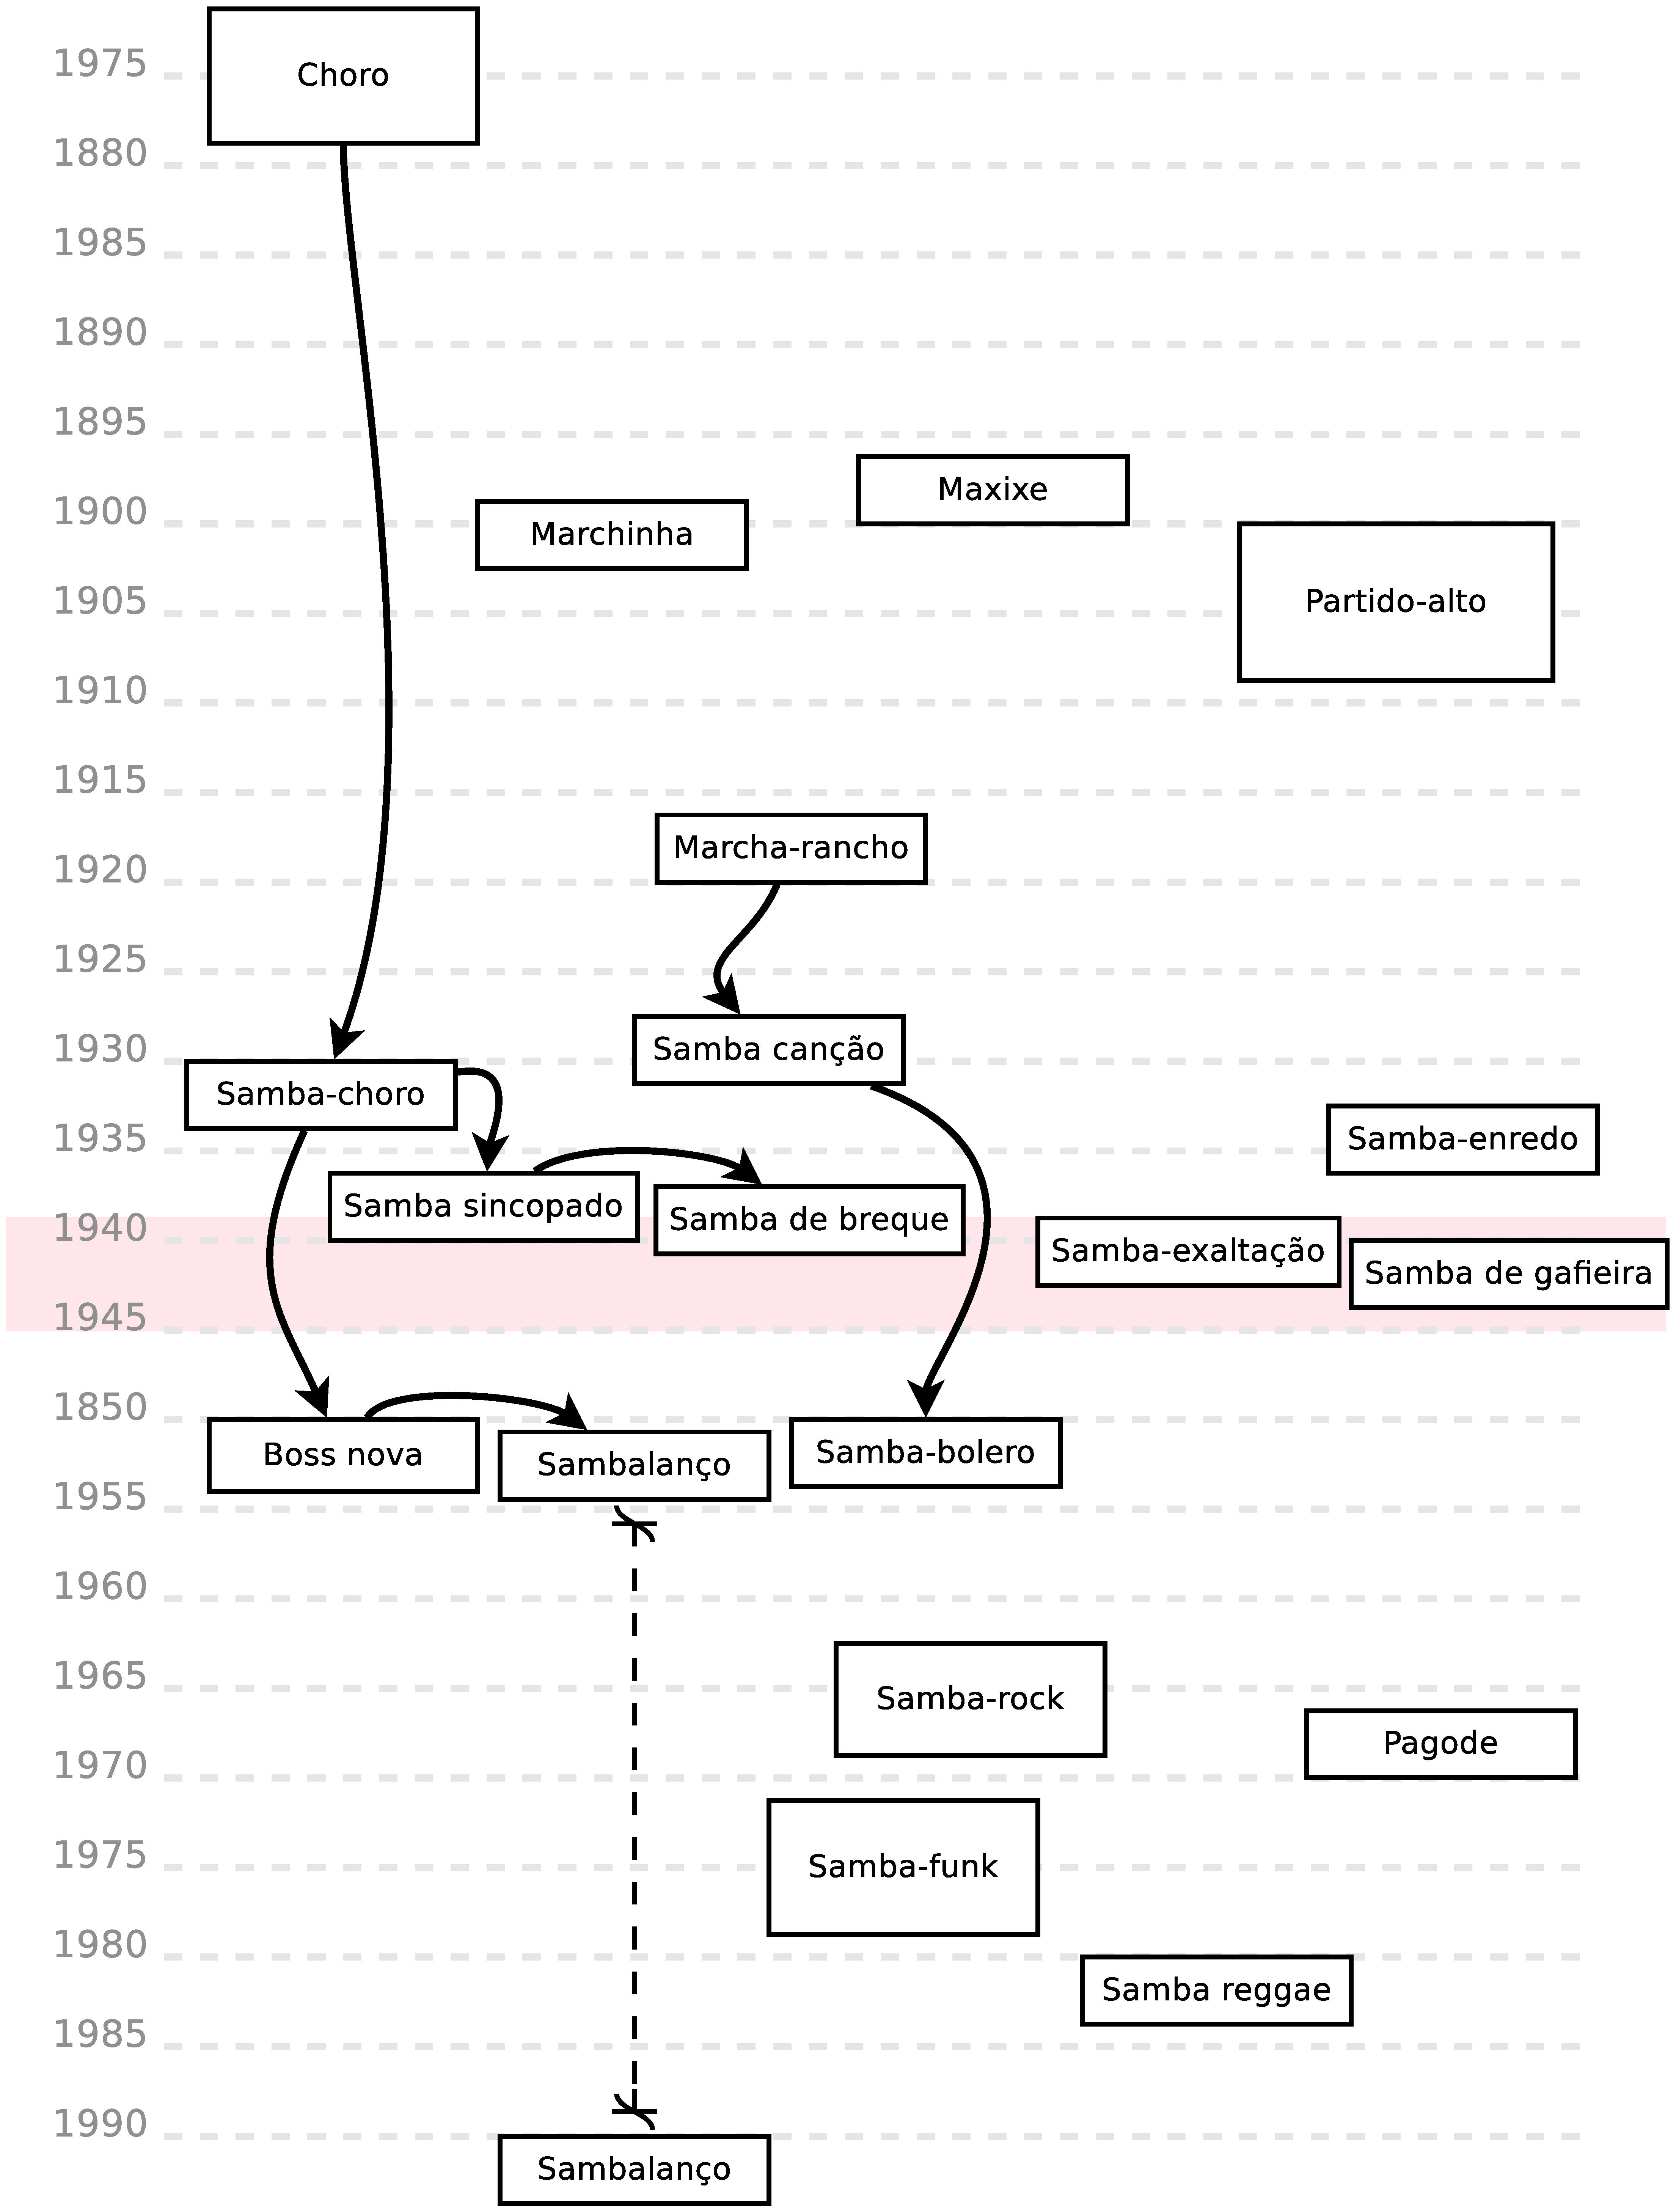
\includegraphics[width=0.95\textwidth]{chapters/cap-historia-musicasamba/musicatimeline.eps}
  \caption{Relação temporal entre os inícios dos subgêneros do samba.}
\label{fig:sambamusicatimeline1}
\end{figure}

%%%%%%%%%%%%%%%%%%%%%%%%%%%%%%%%%%%%%%%%%%%%%%%%%%%%%%%%%%%%%%%%%%%%%%%%%%%%%%%%
%%%%%%%%%%%%%%%%%%%%%%%%%%%%%%%%%%%%%%%%%%%%%%%%%%%%%%%%%%%%%%%%%%%%%%%%%%%%%%%%
\section{Que estilos de dança posso usar no samba (música)?}
\label{subsec:estilosdedanca}
A resposta mais simples poderia ser que, uma pessoa ao ser livre e independente,
pode escolher expressar-se na dança, de forma natural, como esta saia de si mesmo.
Porem, entrando em assuntos mais técnicos, 
e de acordo com os padrões socialmente mais comuns de ser achados atualmente;
existe um grupo de estilos de danças, que por suas caraterísticas, 
são consideradas que se enquadram muito bem na música de alguns subgêneros do samba.

Assim, nas seguintes seções, serão descritos alguns dos estilos de dança para a música do samba,  
que podemos achar nos salões e locais de dança no Brasil;
estes serão agrupados em estilos dançados em pares, e os que se dançam de forma separada. 


%%%%%%%%%%%%%%%%%%%%%%%%%%%%%%%%%%%%%%%%%%%%%%%%%%%%%%%%%%%%%%%%%%%%%%%%%%%%%%%%
\begin{comment}
\subsection{\textcolor{blue}{Estilos dançados em roda}}
\label{subsec:estilosdedancaroda}
Entre os estilos que se dançam em roda, temos:
\begin{description}
\item[Samba de roda:] Samba dançado em roda.
Para mais detalhes ir a página \pageref{ref:Samba-de-roda-danca}.

\item[Samba-de-umbigada:] 
São classificadas com este nome todas as danças que usem a umbigada na sua realização.
Para mais detalhes ir a página \pageref{ref:samba-de-umbigada}.

\item[Batuque (1900s):] Dança em roda onde se intercambiam os dançantes usando o gesto da umbigada.
Para mais detalhes ir a página \pageref{ref:batuquedanca}.

\item[Batucada:] Dança em roda onde se intercambiam os dançantes usando o gesto da pernada.
Para mais detalhes ir a página \pageref{ref:batucadadanca}.
\end{description}
\end{comment}
%%%%%%%%%%%%%%%%%%%%%%%%%%%%%%%%%%%%%%%%%%%%%%%%%%%%%%%%%%%%%%%%%%%%%%%%%%%%%%%%
\subsection{Estilos dançados em pares}
\label{subsec:estilosdedancapares}
Entre os estilos que se dançam a dois, existentes na atualidade, temos \cite[pp. 134]{perna2002samba}:
\begin{description}
\item[Samba de gafieira (dança):] 
\index{Dança!Samba de gafieira}
É uma dança a dois, que pode ser executada na maioria dos subgêneros do samba (música),
tendo exceções em: samba-enredo, samba reggae (música), samba rock (música), 
marcha, marcha-rancho e maxixe (música) \cite[pp. 134]{perna2002samba}.
No seus origens este tipo de dança era chamado de samba-batucada  \cite[pp. 134]{perna2002samba}. 
Para mais detalhes sobre o samba de gafieira, ver Seção \ref{subsec:gafieiradancaestilos}.

\item[Samba liso:] 
\index{Dança!Samba liso}
\index{Dança!Samba caminhado}
Atualmente se dança similarmente ao samba de gafieira, 
porem com um estilo mais elegante, sem ginga né passos de efeito, e dizer é uma dança mais ``lisa'';
se dança bem em : samba-canção, bossa nova e choro \cite[pp. 134]{perna2002samba}.

%%%%%%%%%%%%%%%%%%%%%%%%%%%%%%%
Podemos achar uma referencia interessante ao uso do termo \textbf{samba} e \textbf{liso}  no livro 
``Feitiço decente: Transformações do samba no Rio de Janeiro (1917-1933)'' (2001),
onde se pode intuir a procedência deste nome ou denominação, 
quando se faz referencia a um comentário de João da Baiana sobre o samba-de-umbigada e o samba de roda \cite[pp. 109]{sandroni2001feitico}: 
\begin{citando}
Nós tirávamos um verso e o pessoal sambava, um de cada vez ... 
Um saía para tirar o outro.
Se fosse a ``liso'' era só umbigada, mas se fosse para pegar ``duro'' já era capoiragem. 
\end{citando}
Pelo que no livro se comenta, que para o dançarino solista  escolher a seu sucessor podiam
existir duas modalidades, dependendo do tipo de roda, em ``samba liso'' (com umbigada) ou em ``samba duro'' 
(ou batucada\footnote{No qual a umbigada é substituída por uma pernada \cite[pp. 109]{sandroni2001feitico},
para mais detalhes ir a página \pageref{ref:batuquedanca}.}) \cite[pp. 109]{sandroni2001feitico}.
Esta referencia 
é particularmente interessante, pois como veremos na Seção \ref{cap:sambagafieira},
nos primórdios do samba nas gafieiras, existiam 3 formas em que esta era dançada: samba-canção (dança),
\textbf{samba-batucada} (dança)\footnote{Que 
é o nome com que era conhecido originalmente a atual samba de gafieira \cite[pp. 143]{perna2002samba}.} 
e \textbf{samba-liso} \cite[pp. 143]{perna2002samba};
estas duas últimas, não são as mesmas danças dos samba-de-umbigada, 
e sim novas formas de dançar o samba num ambiente mais civilizado como o salão de dança;
porem, estes nomes conservavam a mesma nomenclatura, na descrição 
da relativa relação à tosquedade dos movimentos.

%%%%%%%%%%%%%%%%%%%%%%%%%%%%%%%
Na ``Hemeroteca Digital Brasileira'' da Fundação Biblioteca Nacional,
não tem-se achado referencias\footnote{ Foram achadas,
2, 5, 3, 1 e 1 referencias brutas para as décadas de 1930, 1940, 1960, 1970 e 1980 respetivamente;
porem, estas não eram relativas ao samba liso de salão ou eram falsos acertos.} 
à frase ``\textbf{samba liso}'', nas décadas de 1930, 1940, 1960, 1970 e 1980;
as referencias achadas correspondem à década de 1950\footnote{Especificamente entre os anos 1950 e 1953.}  
com uma total de 327 referencias;
de todas estas, 326 correspondem à forte campanha 
de marketing do livro
``Como aprender a dançar'' , 
de Gino Forniciari. 
Por exemplo, podemos achar a primeira referencia em ``O Jornal'' (RJ),
do dia 17 de setembro de 1950, onde se pode ler \cite[3ra seção pp. 9]{jornalanunciodanca1}:
\begin{citando}
\begin{center}
Como aprender a dançar\\
4a edição ampliada
\end{center}
Com a nova dança, ``Baião'', \textbf{Samba liso}, e os
últimos passos de Bolero, Rumba, Swing, contendo
120 gráficos 330 passos, facilitando as senhoritas 
e cavalheiros a aprenderem em suas próprias 
casas em 10 dias apenas, no princípio sem
companheiro ou companheira. Método de ritmos modernos
pelo Prof. Gino Fornaciari, 
Diretor e Prof. do ``CURSO PRATICO DE DANÇAS RITZ''.
Aulas particulares, rua da Liberdade, 120.
Preço: Cr\$ 45,00 -- Pedidos pelo reembolso posta 
-- com o autor -- Caixa Postal, 649 -- SÃO PAULO 
\end{citando}
Todos estes anúncios vem na maioria das vesses acompanhados com um desenho como
o mostrado na Figura \ref{fig:desenholivrodanca1}, que indica todos os estilos de dança abordados no livro;
onde se diferencia entre dançar \textbf{samba} e \textbf{samba liso}.
\begin{figure}[h]
  \centering
    \includegraphics[width=0.5\textwidth]{chapters/cap-historia-musicasamba/comoaprenderdancar.jpg}
  \caption{Desenho da publicidade do livro ``Como aprender a dançar'' de Gino Forniciari,
publicado, no dia 17 de fevereiro de 1952, em ``Sport Ilustrado'' \cite[pp. 22]{sportlivropublidanca}.}
\label{fig:desenholivrodanca1}
\end{figure}



%%%%%%%%%%%%%%%%%%%%%%%%%%%%%%%
A outra referencia achada na ``Hemeroteca Digital Brasileira'' da Fundação Biblioteca Nacional,
apara a frase ``samba liso'', na década de 1950, foi a publicada o dia 26 de agosto de 1951,
no ``Diário do Nordeste'' de Caixas do Sul (RS), numa cronica de Walter Brugger da sua viagem por Europa,
num articulo titulado ``Genova! Primeiro Contato com a Europa!'',
onde se pode ler \cite[pp. 10]{nordestesambalisocronica}:
\begin{citando}
Ao nosso lado, numa área 
descoberta uma orquestra tocava para
quem quizesse dançar.
Repentinamente ouvimos uma melodia muito
nossa conhecida. Era o imortal ``Tico-Tico no Fubá''... Todavia,
apesar da melodia correta, o ritmo
era bastante falho. Continuando 
com os ritmos brasileiros, a orquestra 
tocou ainda ``Chiquita Bacana'',
mas em tempo de samba e ``Aquarela do Brasil''.
O que porém nos 
deixou mais atônitos foi o modo como 
era dançado o nosso samba. De 
brasileiro não tinha nada. Pelo que 
vimos, o \textbf{samba ``liso''} lhes é desconhecido 
e cada um procura ``requebrar'' o corpo mais que o outro,
mas de uma forma como nós só 
conhecemos no cinema mexicano. 
O meu amigo dava gostosas risadas e não era para menos,
ante a comicidade do espetáculo, tão 
impossível no Brasil quanto desconhecido para nós.
\end{citando}


%%%%%%%%%%%%%%%%%%%%%%%%%%%%%%%
Outra referencia ao \textbf{samba liso}, pode ser achada no livro ``Manual de Danças Gaúchas'' (1955)
onde se afirma que \cite[pp. 77]{cortesmanual}: 
\begin{citando}
A polquinha, como dança especifica, é executada por pares enlaçados,
mediante passos-de-marcha (É correograficamente  semelhante ao chamado 
\textbf{samba liso} ou \textbf{samba caminhado} dos salões urbanos).
\end{citando}


\item[Samba pagode:] 
\index{Dança!Samba pagode}
É um estilo de dança a dois, originário de São Paulo, 
é uma dança com poucos deslocamentos \cite[pp. 134]{perna2002samba}.
É um estilo de dança adaptado para ser dançado com o pagode paulista,
também chamado como Sambalanço\footnote{Ver página \pageref{ref:sambalanco}}.
%% https://www.youtube.com/watch?v=SfvoiXOGPn4
Ao igual que o sambalanço teve duas épocas com estilos musicais diferentes,
a dança \textbf{samba pagode}, sofreu também transformações acompanhando essas tendencias.
Podem-se observar atualmente 3 tipos de passo base: 
%% https://www.youtube.com/watch?v=rq1uhNXySds 
%% https://www.youtube.com/watch?v=SfvoiXOGPn4

O miudinho, que é um passo que se realiza abraçado com o par e de forma espelhada com este,
onde se executam 3 twist\footnote{É importante ter um sapato que deslise bem.} no lugar, 
só trocando de peso entre os pés, seguindo um ritmo, rápido-rápido-lento;
este movimento se executa simetricamente duas vesses para formar um ciclo completo,  
uma vez iniciando com o peso do corpo para o pé direito\footnote{Quando o primeiro twist é horário.} e a outra com o esquerdo.

O passo básico lateral, se realiza abraçado com o par  e de forma espelhada com este, 
é similar ao passo básico de capoeira,
ou a base aberta do forró\footnote{Só que aqui é abraçados.},
onde se produzem 3 movimento seguindo um ritmo, rápido-rápido-lento,
no primeiro momento, um pé vai para atrás, 
no segundo o outro ajeita sua posição deslocando-se levemente, 
procurando o centro e o equilíbrio do par dançante, e
no terceiro o pé que estava atrás volta ao lado do outro,
este movimento se executa simetricamente duas vesses para formar um ciclo completo,  
uma vez iniciando com pé direito e a outra com o esquerdo.
Este movimento é interessante para fazer deslocamento, 
que são realizados principalmente nesse primeiro movimento com o pé atrás, 
só que agora apontando para uma direção especifica.

A caidinha, se realiza abraçado com o par, 
este passo é similar ao picadilho (picadinho) de samba de gafieira,
porem com um deslocamento similar ao repique do forró;
no pagode paulista este movimento se executa seguindo um ritmo, rápido-rápido-lento,
onde o seguidor faz um movimento similar ao miudinho antes mencionado,
enquanto que o condutor tem uma liberdade criativa no 
seu movimento\footnote{O mesmo que acontece no picadilho de samba de gafieira.} 
enquanto respeite o ritmo, rápido-rápido-lento.


\item[Samba rock:] 
\index{Dança!Samba rock}
É um estilo de dança a dois, realizado nos bailes ``black'' paulistas desde a década de 1960, 
sendo esta uma dança variante das danças do swing/rock e parente do soltinho carioca \cite[pp. 135]{perna2002samba}.
se dança bem em: Swing, samba rock (música), samba com suingue e samba-funk \cite[pp. 135,138]{perna2002samba}.
O samba rock se dança de mão dadas, e se carateriza por ter muitas voltas,
executadas na maior parte de vesses pelas  seguidores;
porem, é uma dança estacionaria pois os dançantes rara vez se deslocam pelo salão, 
e pelo contrario ficam trabalhando seus passos num mesmo lugar  \cite[pp. 135,138]{perna2002samba}.
Quando um espectador externo vê esta dança perceberá muitas figuras usando só os braços,
com enrosques, voltas, enlaces, etc.
Enquanto os pés de ambos dançarinos fazem uma mesma marcação, num constante e repetitivo rápido-rápido-lento,
caminhando unicamente sobre um circulo imaginário no chão, uma vez em sentido horário e outra em anti-horário.

\item[Samba funkeado:] 
\index{Dança!Samba funkeado}
Também é chamado de estilo Jimmy de Oliveira ou simplesmente  samba Jimmy, 
em aluição a seu criador.
Este estilo de dança a dois foi criado no ano de 1998.
Com muito esforço Jimmy, num período aproximado de 6 meses, 
criou a estrutura da dança, desde iniciante ate avançado;
no ano de 1999 ele  chamou a esse estilo como ``samba quebrado'';  
posteriormente renomeou  para ``samba Jimmy'', 
recebeu algumas criticas e no ano 2001 decidiu renomeá-lo para ``samba funk'',
porem isto trouxe confusões   ao ser associado com a música funk, existente em Rio de Janeiro,
muito distante da proposta dele, e
finalmente a meados do 2005 ele decidiu chamá-lo ``samba funkeado''  \cite{sambafunkeadoJimmyDeOliveiraPart1}.
A Figura \ref{fig:funkeadocrono1} mostra a cronologia de nomes para este estilo.
\begin{figure}[h]
  \centering
    \includegraphics[width=0.85\textwidth]{chapters/cap-historia-musicasamba/sambafunkeado.eps}
  \caption{Cronologia dos nomes para samba funkeado.}
\label{fig:funkeadocrono1}
\end{figure}

O estilo foi criado para, em palavras de Jimmy: ``contribuir em função da música'', 
numa tentativa de agregar movimento em coerência como as músicas que ele gostava;
sendo estas interpretadas por:
Djavan, Jorge Ben Jor, Tim Maia, Leny Andrade \cite{sambafunkeadoJimmyDeOliveiraPart1}, que em seu momento, 
presentaram músicas de bossa nova ou que eram influenciadas pelo jazz, funk norte-americano ou ``black music'' \cite{sambafunkeadoJimmyDeOliveiraPart1} \cite{sambafunkeadoJimmyDeOliveiraPart3},
Jimmy indica que seu estilo procura ir em função da música escutada no brasil, 
e que a maioria da música atual é influenciada pelo funk norte-americano;
como a música de: João Sabiá. 

O samba funkeado pode ser dançado em gêneros como ``black music'',
em pagodes funkeados (Sorriso maroto, Netinho de Paula, pixote, etc.), em sambas com influencia do jazz \cite{sambafunkeadoJimmyDeOliveiraPart3}, etc. 

O samba funkeado tem 3 tendencias ou estruturas  \cite{sambafunkeadoJimmyDeOliveiraPart2}:
\begin{itemize}
\item \textbf{Samba funkeado}, primigênio.
\item \textbf{Samba funkeado fragmentado}; exemplo: um movimento que é de sentar, que gastaria um tempo, 
passa a ter ate 3 tempos; é dizer, fragmenta os movimentos. 
O fragmentado também permite dançar com movimentações em contrapeso no par de dança.
\item \textbf{Samba funkeado samsurf}, com uma postura mais curvada.
\end{itemize}

%e em seu ídolo Michael Jackson \cite{sambafunkeadoJimmyDeOliveira2}.
 

\item[Samba internacional:] 
\index{Dança!Samba internacional}
É um estilo de dança a dois, influenciado pelo maxixe;
se dança principalmente fora do Brasil e existem basicamente dois estilos: 
o estilo internacional e o estilo norte-americano (EE.UU.) \cite[pp. 134-135]{perna2002samba}.

O samba introduzida a EE.UU. é uma dança de salão muito animada, 
com música de ritmo alegre, que sugere um estilo de movimento que pode
chegar a ser tão turbulento quanto os movimentos do Jive.
O padrão de passos básicos é similar aos achados no Fox-Trot e o Waltz,
sendo estes: fwd-swd-close ... bwd-swd-close; e
tem passos com tempos que seguem uma sequência: 
quick-quick-slow\footnote{Rápido-rápido-lento.} ... quick-quick-slow \cite{parson2016ballroom}.

Observando os campeonatos internacionais onde este estilo é usado, 
se percebe que o samba internacional é dançado em qualquer estilo musical que
tenha sotaque ou de a impressão de ter raiz afro-latina.

\end{description}~

A Figura \ref{fig:sambadavavsmusica} mostra as relações entre os estilos de dança a dois atuais,
 e os subgêneros do samba \cite[pp. 134-138]{perna2002samba}.

\begin{figure}[h]
  \centering
    \includegraphics[width=0.6\textwidth]{chapters/cap-historia-musicasamba/dancavcmusica.eps}
  \caption{Relações entre os estilos de dança a dois e os subgêneros do samba.}
\label{fig:sambadavavsmusica}
\end{figure}

%%%%%%%%%%%%%%%%%%%%%%%%%%%%%%%%%%%%%%%%%%%%%%%%%%%%%%%%%%%%%%%%%%%%%%%%%%%%%%%%
\subsection{Estilos dançados individualmente ou separados }
Entre os estilos que se dançam de forma separada temos \cite[pp. 134]{perna2002samba}:
\begin{description}
\item[Samba reggae  (dança):] Este estilo de samba que se dança separado, 
é uma dança baiana também conhecida como axé-dance, samba baiano ou pagode baiano,
se dança em samba reggae (música) \cite[pp. 134]{perna2002samba}.

\item[Samba no pé:] É o estilo usado nas quadras das escolas de samba,
se dança bem em estilos musicais como: 
samba enredo ou em qualquer samba rápido  \cite[pp. 134]{perna2002samba}.

\item[Marcha de carnaval:] É uma dança própria do carnaval para se dançar em cordões.
se dança bem em: marchas, marchas-rancho e samba-enredo lentos  \cite[pp. 135]{perna2002samba}.

\end{description}
~

A Figura \ref{fig:sambadavavsmusicaseparado} mostra as relações existentes, 
entre os estilos de dança que se dançam separados e alguns subgêneros do samba  \cite[pp. 134-138]{perna2002samba}.

\begin{figure}[h]
  \centering
    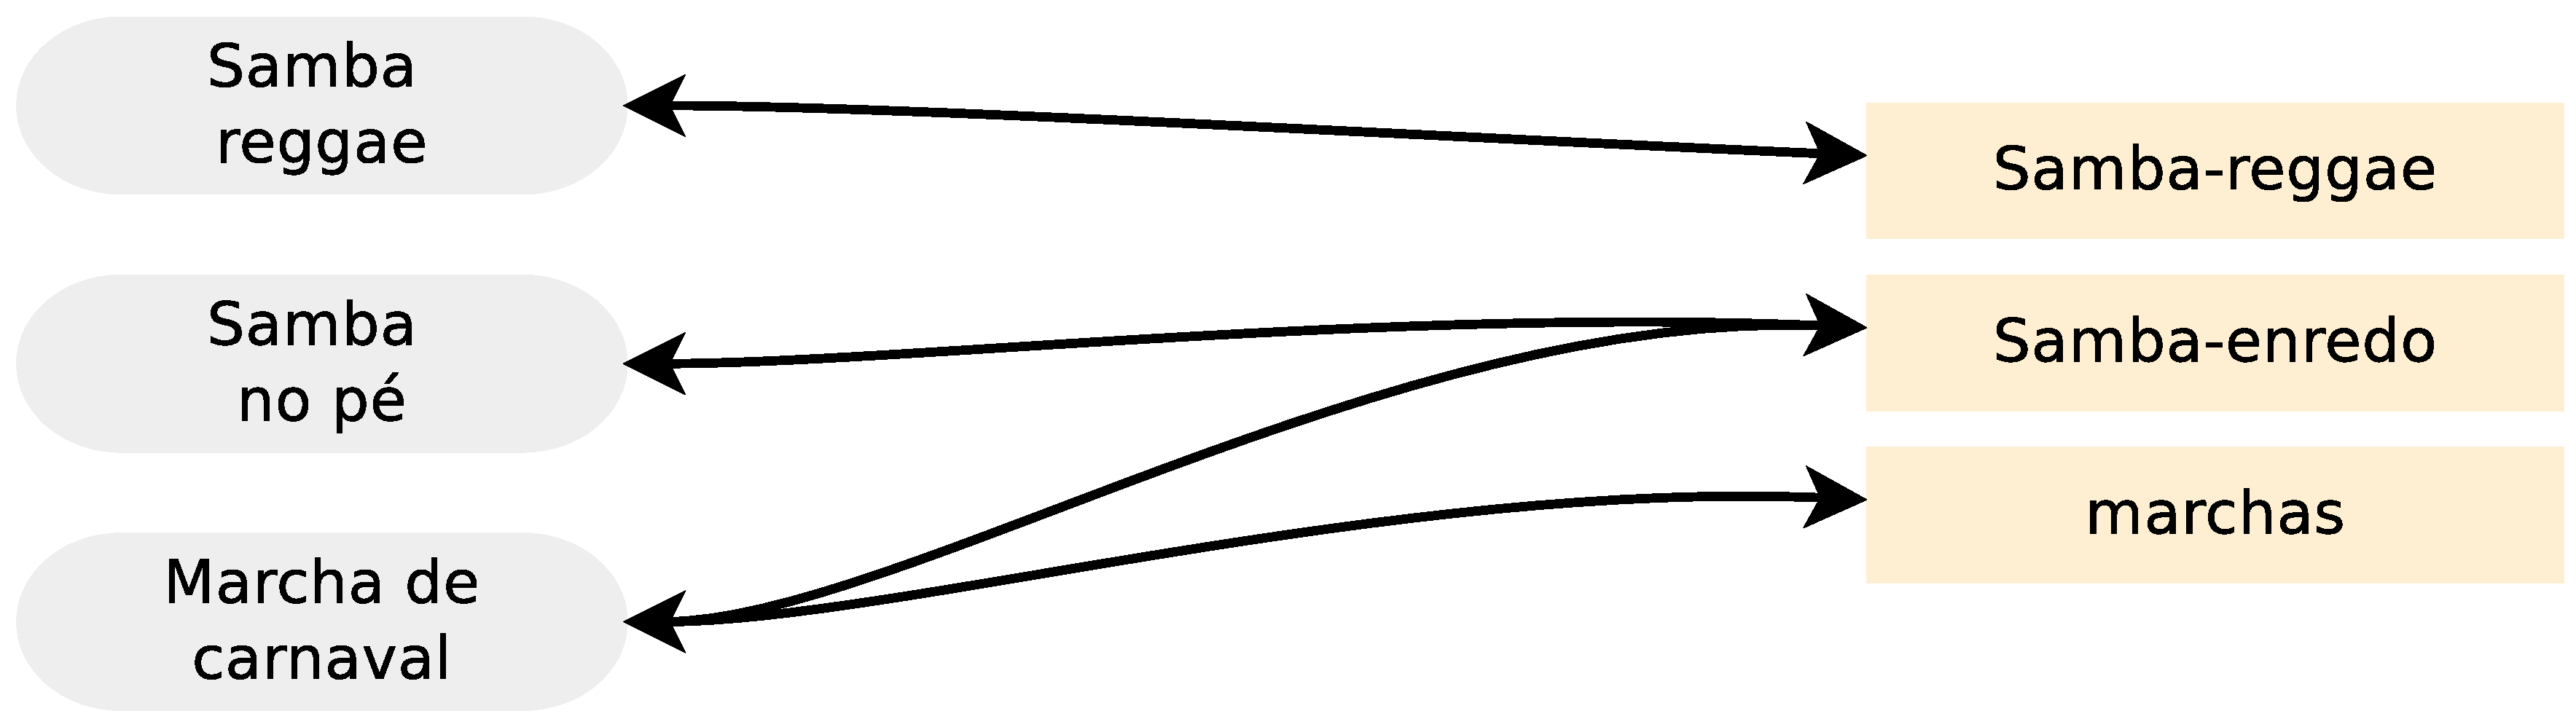
\includegraphics[width=0.6\textwidth]{chapters/cap-historia-musicasamba/dancavcmusicaseparado.eps}
  \caption{Relações entre os estilos de dança (separados) e os subgêneros do samba.}
\label{fig:sambadavavsmusicaseparado}
\end{figure}


%%%%%%%%%%%%%%%%%%%%%%%%%%%%%%%%%%%%%%%%%%%%%%%%%%%%%%%%%%%%%%%%%%%%%%%%%%%%%%%%
%% CAPITULO
%%%%%%%%%%%%%%%%%%%%%%%%%%%%%%%%%%%%%%%%%%%%%%%%%%%%%%%%%%%%%%%%%%%%%%%%%%%%%%%%
\chapterimage{chapter_head_2.pdf} % Chapter heading image

\chapter{\textcolor{green}{Historia do samba de gafieira  (dança)}}
\label{cap:sambagafieira}
\index{Dança!Samba de gafieira}


\section{Lundum (a dança do lundu)} 
\label{sec:lundu}
\index{Dança!Lundu}
O lundum é o estilo de dança que lhe corresponde ao gênero musical lundu \cite[pp. 18]{perna2002samba}.
Esta é uma dança, brasileira, de roda e umbigada; e teve sua origem no batuque dos bantos africanos,
e provavelmente foi trazida de Angola pelos escravos na segunda metade do século XVIII \cite[pp. 48]{tinhorao1986pequena} \cite[pp. 188]{dourado2004dicionario},
sendo que as primeiras referencias conhecidas se remontam a 1780 
descrevendo a dança como indecente e licenciosa \cite[pp. 51]{tinhorao1986pequena} \cite[pp. 19]{perna2002samba}.
Posteriormente foi introduzida aos salões das cortes do Brasil e Portugal, 
dançado elegantemente nas cortes, porem indecentemente pela gente comum   \cite[pp. 19]{perna2002samba} \cite[pp. 188]{dourado2004dicionario}.
No Brasil esta dança teve influencias da ``Modinha''(Portuguesa) e do ``Fandango''(Espanhol) \cite[pp. 188]{dourado2004dicionario}.

A partir de 1820 o lundum é apresentado, como dança de caráter libidinoso nos teatros de Baia, Pernambuco e Rio de Janeiro;
onde eram representados pequenos quadros cômicos, 
mostrando a umbigada e outras caraterísticas da dança \cite[pp. 19]{perna2002samba}.


\section{Maxixe (dança)}
\label{sec:maxixe}
\index{Dança!Maxixe}
Esta é uma dança urbana afro-brasileira \cite[pp. 4]{musicasambavariasdef1}, 
em compasso binário, surgida em Rio de Janeiro, 
na Cidade Nova e nos cabarés de Lapa \cite[pp. 465]{marcondes1977enciclopedia}  \cite[pp. 198]{dourado2004dicionario}, 
aproximadamente entre 1870 e 1880 \cite[pp. 58]{tinhorao1986pequena} \cite[pp. 465]{marcondes1977enciclopedia}  \cite[pp. 62]{reinato2010musica}.

A dança era considerada de baixe ralé pela sociedade local, 
pois era entendida como um modismo indecente das classes baixas, imoral como o Lundu \cite[pp. 198]{dourado2004dicionario}.
Esta dança recebeu influencias da polca \cite[pp. 198]{dourado2004dicionario} e 
da Habanera \cite[pp. 62]{reinato2010musica}.


O maxixe tinha uma boa quantidade de passos como: 
\begin{itemize} 
\item parafuso  \cite[pp. 68, 93, 129]{efege1974maxixe} \cite[pp. 465]{marcondes1977enciclopedia} \cite[pp. 62]{tinhorao1986pequena}, 
\item janela  \cite[pp. 129]{efege1974maxixe},
\item jocotó \cite[pp. 83, 96, 173]{efege1974maxixe},
\item saca-rolha \cite[pp. 465]{marcondes1977enciclopedia}, 
\item balão \cite[pp. 93]{efege1974maxixe} \cite[pp. 465]{marcondes1977enciclopedia}, 
\item balão apagado \cite[pp. 68]{efege1974maxixe} \cite[aproximadamente min. 11:35]{MaxixeDocumentario1},
\item balão caindo  \cite[pp. 129, 131]{efege1974maxixe} \cite[pp. 62]{tinhorao1986pequena},
\item corta-jaca  \cite[pp. 131]{efege1974maxixe},
\item urubu malandro  \cite[pp. 131]{efege1974maxixe},
\item sino \cite[pp. 68]{efege1974maxixe}, 
\item carrapeta  \cite[pp. 465]{marcondes1977enciclopedia}, 
\item corta-capim \cite[pp. 465]{marcondes1977enciclopedia} \cite[pp. 62]{tinhorao1986pequena}, 
\item cobrinha \cite[pp. 62]{tinhorao1986pequena},
\item maxixe puladinho \cite[pp. 177]{1920revista},
\item etc. 
\end{itemize}
Num principio o maxixe era dançado nas músicas de tango, havanera, polca e lundu; 
e só foi ate o final do século XIX que ganhou uma música com gênero próprio \cite[pp. 465]{marcondes1977enciclopedia},
criado pela fusão da polca, o schottisch e a mazurca \cite[pp. 58]{tinhorao1986pequena}.

No inícios do século XX o maxixe foi exportado e dançado na Europa, atingindo um grande sucesso, 
chegando a ser apresentado pelo dançarino ``Duque'' em Paris (1914) e em Londres (1922) \cite[pp. 465]{marcondes1977enciclopedia}.
Este dançarino é considerado o civilizador do maxixe \cite[pp. 129]{efege1974maxixe}.

Uma explicação muito interessante do maxixe é cantada pela atriz, Aurélia Delorme,
numa representação num quadro de revista, interpretando  ``Maxixe Aristocrático'' (1904, José Nunes), 
que arrancava aplausos e provocava pedidos de bis;
o seguinte texto indica sua pauta \cite[pp. 80-81]{efege1974maxixe} \cite{REIS2003}: 
\begin{citando}
O maxixe tem ciência,\\
ou pelo menos tem arte.\\
Para haver proficiência\\
basta mexer certa parte.\\
Pois o próprio Padre Santo,\\
sabendo o gosto que tem,\\
virá de Roma ao Brasil\\
dançar maxixe também.\\ 
\end{citando}



\section{\textcolor{green}{Samba de gafieira (dança)}}
\index{Dança!Samba de gafieira}
O samba de gafieira, como dança, descende principalmente do maxixe (dança),
que a sua vez foi gerado  pela união do  lundu, 
a polca e outras danças europeias.
Assim, misturando o maxixe com a ginga, e o ritmo de outras danças africanas, 
é que se obteve o que agora chamaríamos como samba de gafieira (primigênio)\footnote{
Primitivo; primordial; o primeiro da sua espécie. = PRIMÍGENO \cite{priberamprimigenio}.
} \cite[pp. 139]{perna2002samba}.




A Figura \ref{fig:formuladosambagafieira} mostra a árvore genealógico do samba de gafieira (primigênio),
visto quando o samba fez sua aparição nos salões de dança denominados gafieiras.
\begin{figure}[h]
  \centering
  \begin{subfigure}[b]{0.535\textwidth}
    \centering
    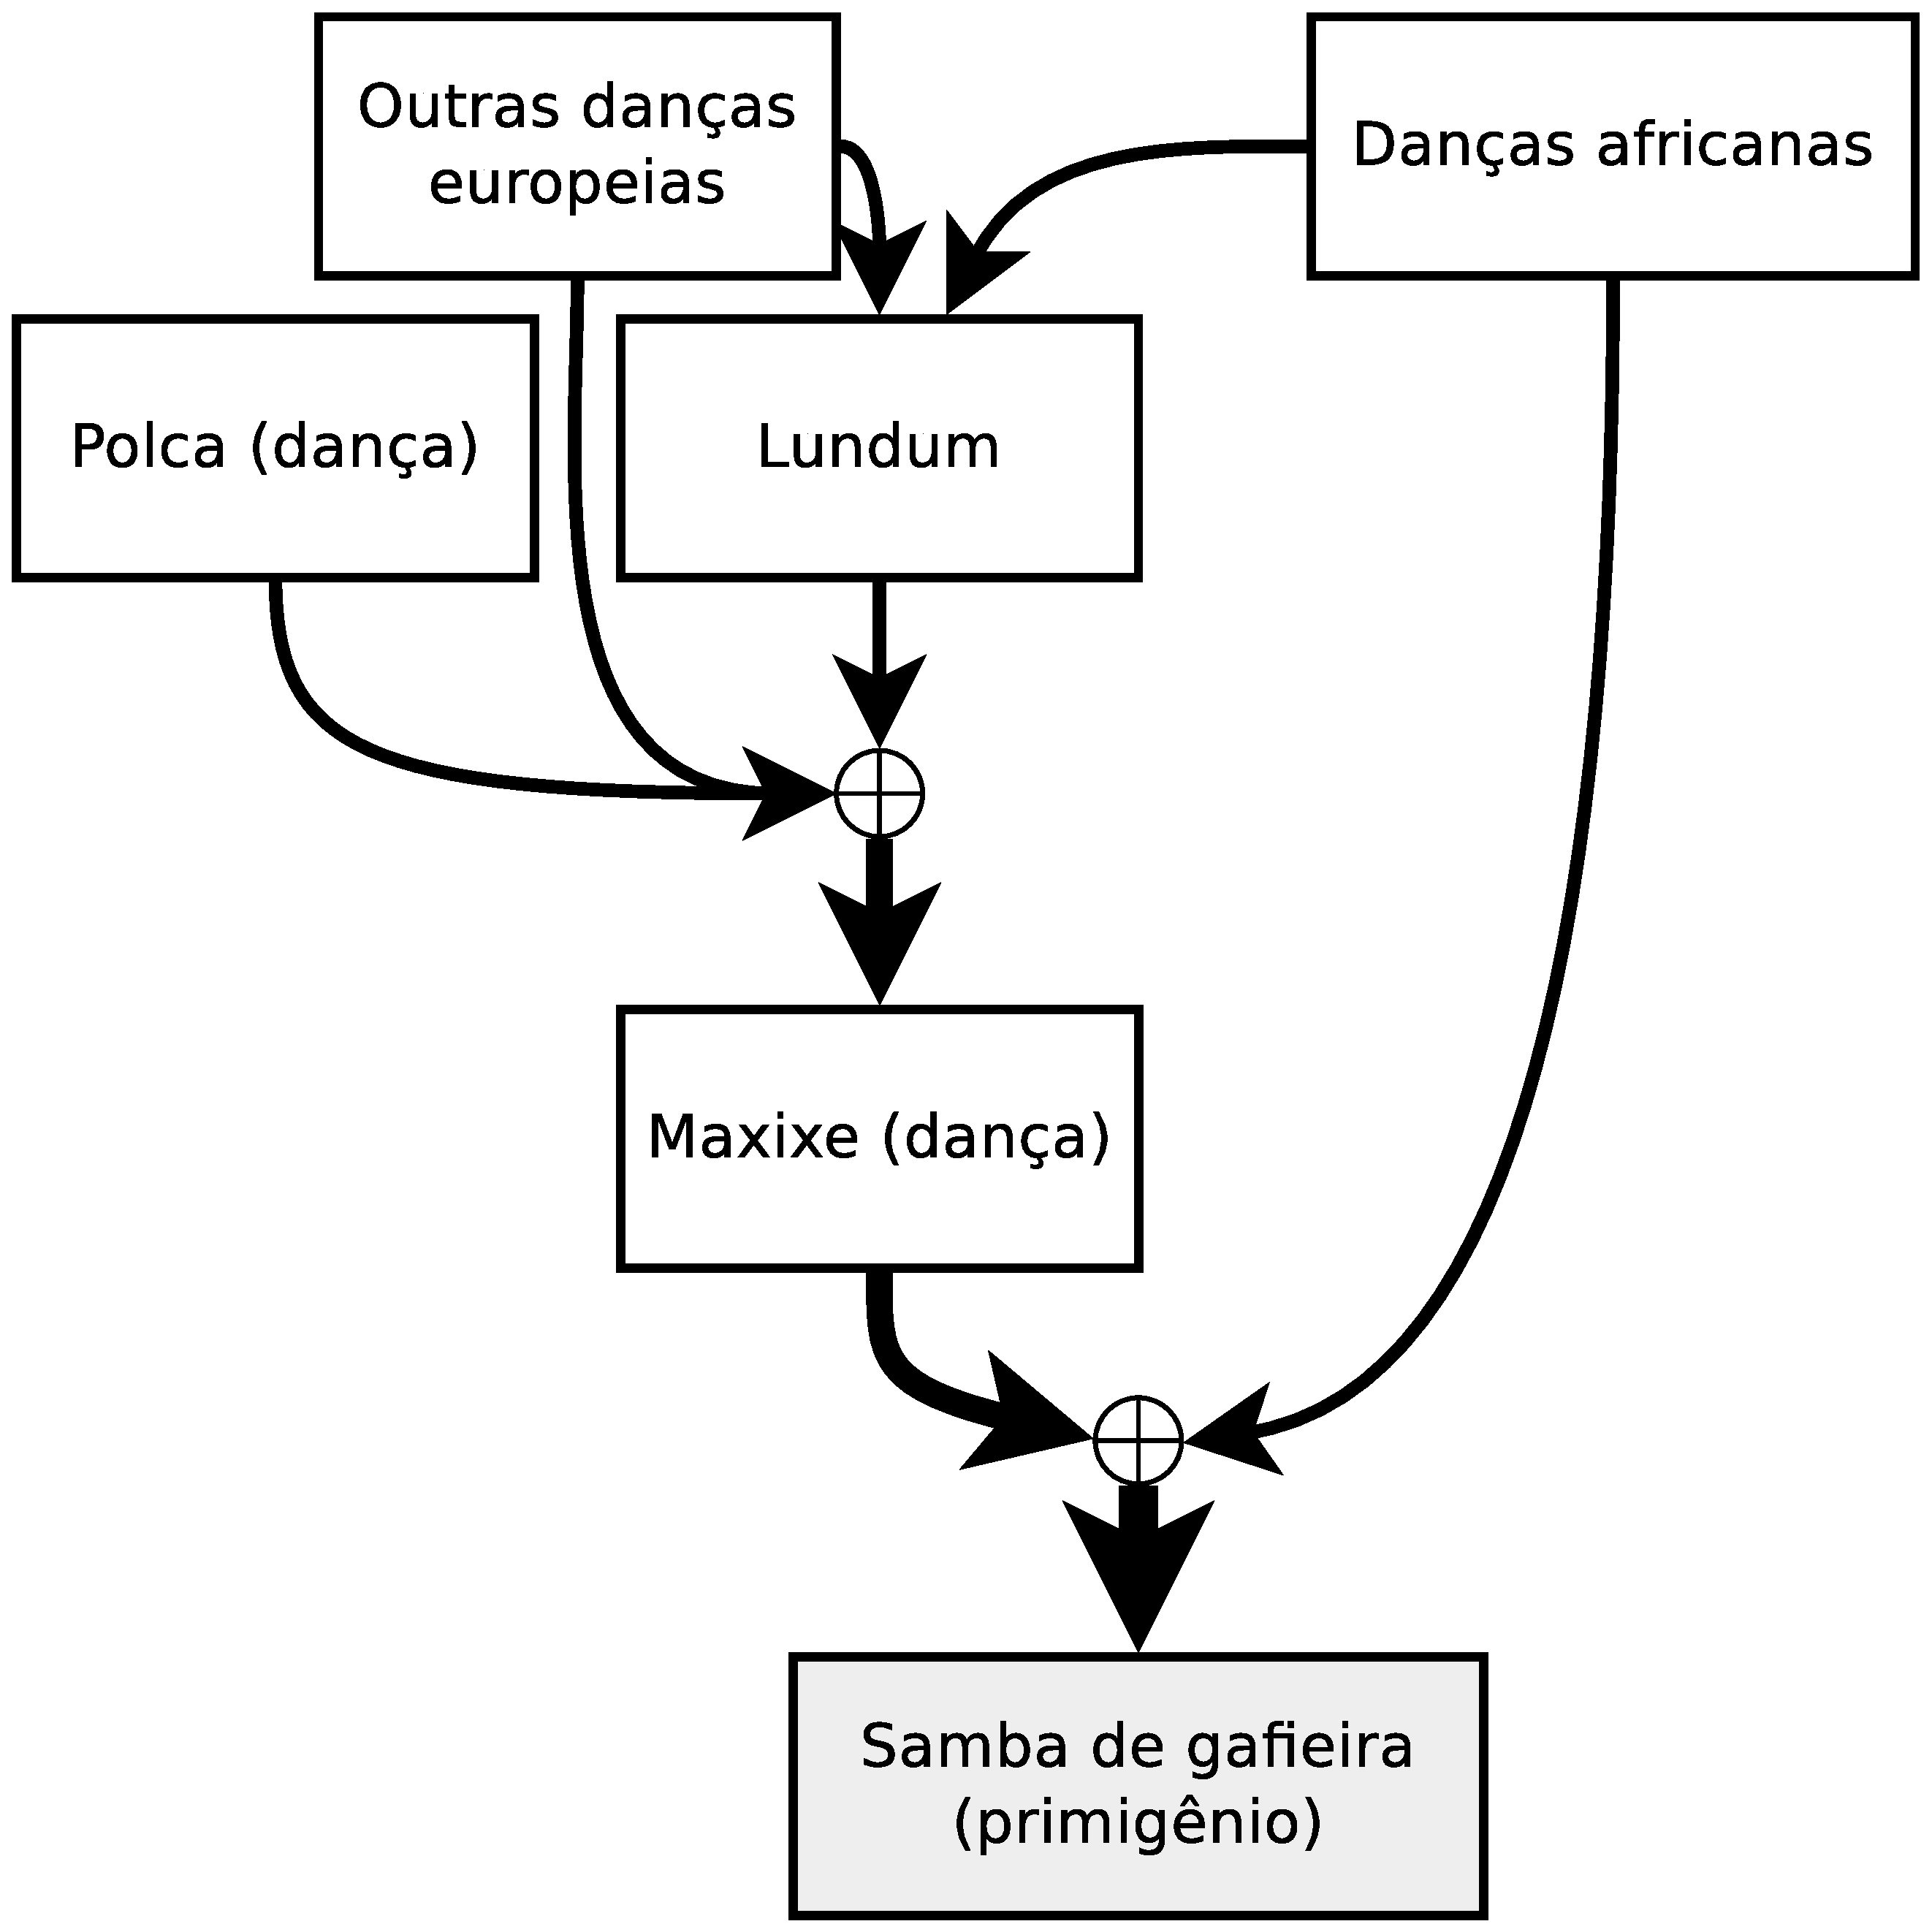
\includegraphics[width=\textwidth]{chapters/cap-historia-sambagafieira/sambagafieiraformula.eps}
    \caption{Formação do samba de gafieira (primigênio).}
    \label{fig:formuladosambagafieira}
  \end{subfigure}
  \begin{subfigure}[b]{0.385\textwidth}
    \centering
    \includegraphics[width=\textwidth]{chapters/cap-historia-sambagafieira/sambagafieiraformula2.eps}
    \caption{Formação do samba de gafieira (atual).}
    \label{fig:formuladosambagafieira2}
  \end{subfigure}
\caption{Formula da criação do samba de gafieira.}
\label{fig:formuladosambagafieiraall}
\end{figure}


O aparecimento do samba nos salões de dança, 
foi um grande impacto para as pessoas que frequentavam estes lugares;
sendo considerado um ritmo novo e ligeiro,
que desagradou aos bailarinos de maior idade e menos ágeis \cite[pp. 6 - cad. B]{entrevistajuliojournalbrasil1}.
O senhor, Júlio Simões, Administrador da ``Kananga do Japão'' e posteriormente socio
do ``Elite Club'', chegou a temer pelo futuro do seus empreendimentos; porem, para sorte dele, 
o samba fez muito sucesso no Elite,
e passou a ser considerado vestibular indispensável para qualquer pessoa que pretendesse ser bailarino, 
compositor ou instrumentista \cite[pp. 6 - cad. B]{entrevistajuliojournalbrasil1}.

\PRLsep{Samba nos salões em 1940}

Pode-se estabelecer o ingresso do samba, aos salões de dança, entre os anos de 1930 e 1940 \cite[pp. 140]{perna2002samba}.
Em palavras do Prof. de dança Gino Fornaciari, 
o samba dessa época tinha um aprecido com o Foxtrot e a Rumba, se dançava num compasso binario,
sendo esta dança a preferida do mulato brasileiro
%sendo este estilo de dança de salão que nasceu na \hyperref[ref:batucadadanca]{\textbf{batucada}} 
%de pretos que descia à cidade na epoca das festas 
\cite[pp. 50]{fornaciari1947aprender}.
Para a decada de 1940 o samba carioca de salão \cite[pp. 50]{fornaciari1947aprender},  já tinha ganhado muita força nos salões,
e podia-se ver 3 modalidades de dançar o samba \cite[pp. 58]{freitas1959danca} \cite[pp. 142-143]{perna2002samba} 
\cite[pp. 51]{fornaciari1947aprender}:
\begin{itemize}
\item \textbf{Samba-canção (dança)},
\index{Dança!Samba-canção} 
Era uma dança com balanços aos lados que se executava de joelhos flexionados,
usando dois movimentos por cada compasso binario \cite[pp. 58]{freitas1959danca} 
\cite[pp. 51]{fornaciari1947aprender} \cite[pp. 143]{perna2002samba}; 
na atualidade é um modo de dança extinto \cite[pp. 143]{perna2002samba}.

Sobre os passos usados entre 1947-1959, 
na Figura \ref{fig:samba-cancao-basico-frente} se mostra o passo básico para a frente do samba-canção,
e na  Figura \ref{fig:samba-cancao-basico-frente} o mesmo movimento para trás;
em ambos casos se usa os 2 movimentos antes mencionados, e a cor cinza indica a posição inicial \cite[pp. 51]{fornaciari1947aprender} \cite[pp. 59-60]{freitas1959danca}. 
\begin{figure}[h]
    \centering
    \begin{subfigure}[b]{0.4\textwidth}
        \centering
        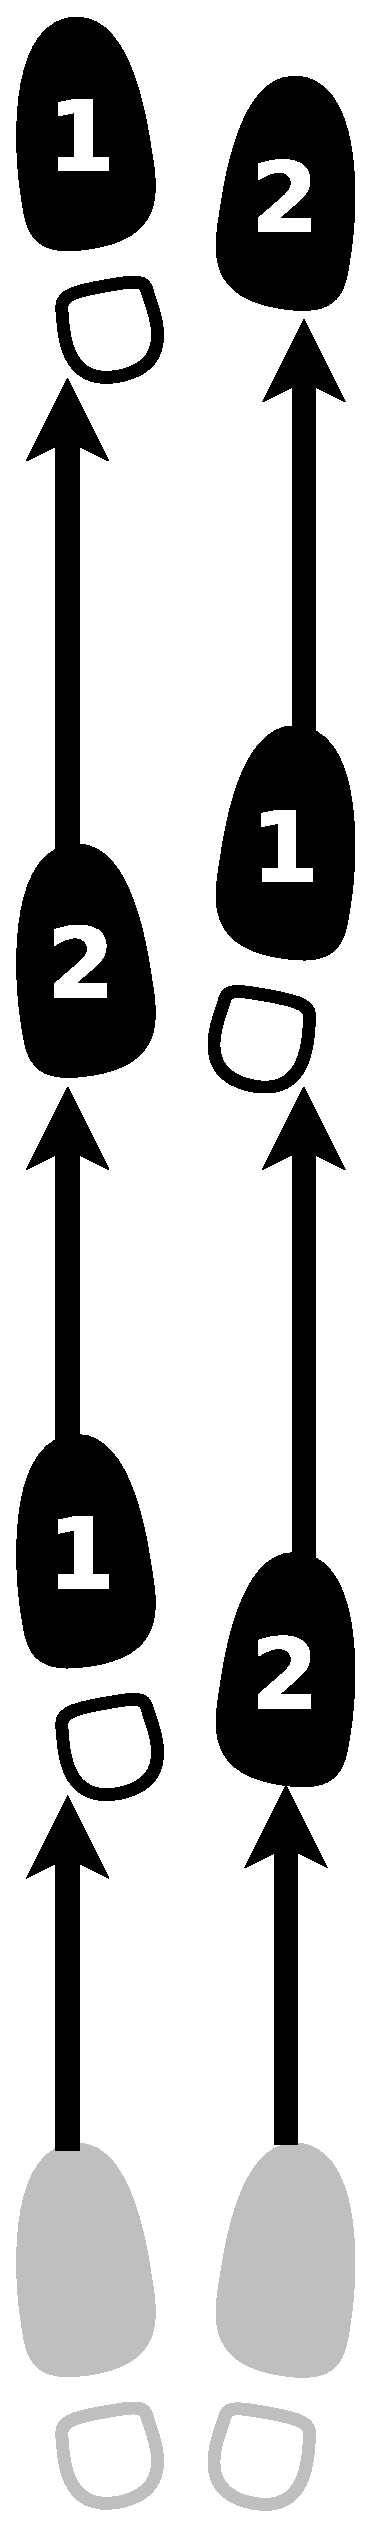
\includegraphics[width=0.25\textwidth]{chapters/cap-historia-sambagafieira/samba-cancao-basico-frente.eps}
        \caption{Passo básico para a frente.}
        \label{fig:samba-cancao-basico-frente}
    \end{subfigure}
    ~ %add desired spacing between images, e. g. ~, \quad, \qquad, \hfill etc. 
      %(or a blank line to force the subfigure onto a new line)
    \begin{subfigure}[b]{0.4\textwidth}
        \centering
	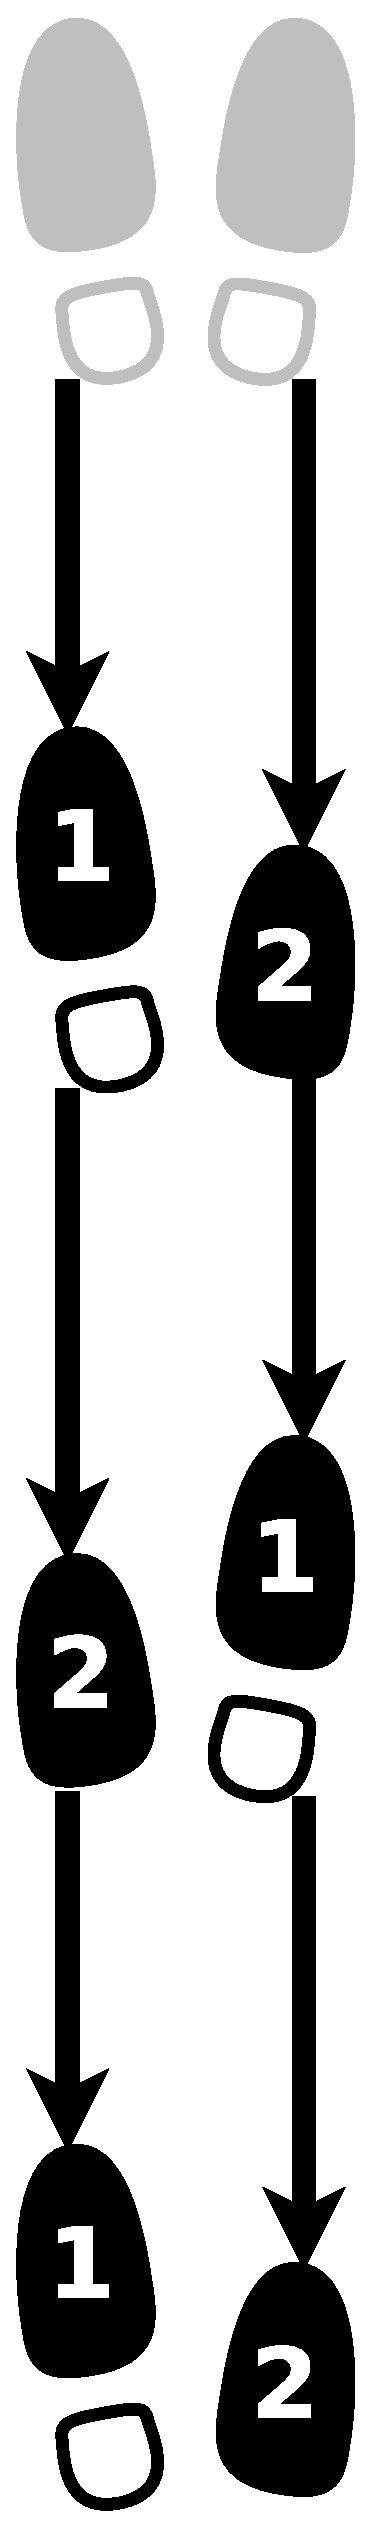
\includegraphics[width=0.25\textwidth]{chapters/cap-historia-sambagafieira/samba-cancao-basico-tras.eps}
        \caption{Passo básico para trás.}
        \label{fig:samba-cancao-basico-tras}
    \end{subfigure}
    \caption{Samba-canção da década de 1959.}\label{fig:samba-cancao-basico}
\end{figure}


\item \textbf{Samba-batucada},
\index{Dança!Samba-batucada} 

O samba-batucada é o samba de gafieira (primigênio) \cite[pp. 143]{perna2002samba}.

Existe uma menção sobre este estilo no ``Jornal do Brasil'', no dia 9 de janeiro de 1938,
onde se indica \cite[pp. 4]{musicasambavariasdef1}:
\begin{citando}%%
Tentativas isoladas de puro 
snobismo e ás vezes de compreensão 
inexata da origem da 
musica e dansa, chamam-no de samba jongo, \textbf{samba batucada} ou
pretendem mistura-lo com o fox, -- samba fox ou com a rumba samba-rumba.
\end{citando}



No livro ``Feitiço decente: Transformações do samba no Rio de Janeiro (1917-1933)'' (2001),
se comenta, sobre uma roda do samba, que para o dançarino solista  escolher a seu sucessor podiam
existir duas modalidades, em ``samba liso'' (com umbigada) ou em ``samba duro'' 
(ou batucada) no qual a umbigada é substituída por uma pernada \cite[pp. 109]{sandroni2001feitico}.
Deste comentário pode ser deduzido de onde vem a denominação \textbf{samba-batucada}, 
que surgiu nos salões de dança apos 1930; pois já existia uma tradição na nomenclatura,
em separar duas formas de dançar uma mais leve (a liso) e uma mais brusca (batucada);
assim, a variante de samba no salão que tendia a explorar movimentos muito  gingados, bruscos ou rápidos,
foi nomeado de samba-batucada, em contraposição ao samba liso onde né se flexionavam os joelhos pra dançar.  



O samba-batucada era, entre 1947 e 1959, uma dança com balanços que se dançava de joelhos flexionados  
e usava 3 movimentos por compasso, que exigia uma maior rapidez, 
especialmente no terceiro movimento que é mais rápido e curto \cite[pp. 61]{fornaciari1947aprender} \cite[pp. 58,66]{freitas1959danca};
seguindo essa descrição, 
o mais provável é que se dançara seguindo uma distribuição de tempos,
parecida ao ritmo do baião de 1949 \cite{CORTES2014}, como pode-se ver na Figura \ref{time:sambabatucada}.
\begin{figure}[H]
\centering
\begin{abc}[name=abc-sambabatucada]
X: 1 % start of header
K: C stafflines=1 % scale: C major
M: 2/4 %meter - compasso
%Q:1/4=100
V:1 clef=perc stem=up %name="TC"   sname="TC"
[V:1] |:  B3/2 B/2 B1 z1 | B3/2 B/2 B1 z1 | B3/2 B/2 B1 z1 | B3/2 B/2 B1 z1 :|
w:        P1   P2  P3      P1   P2  P3      P1   P2  P3      P1   P2  P3
\end{abc}
\caption{Frase de 8 tempos onde P1, P2 e P3 indicam o pé 1, 2 e 3 respetivamente.}
\label{time:sambabatucada}
\end{figure}

Sobre os passos usados na época, 
na Figura \ref{fig:samba-batucada-basico-frente} se mostra o passo básico para a frente do samba-batucada,
e na  Figura \ref{fig:samba-batucada-basico-tras} o mesmo movimento para trás;
em ambos casos se usa os 3 movimentos antes mencionados, e a cor cinza indica a posição inicial \cite[pp. 61-62]{fornaciari1947aprender} \cite[pp. 63]{freitas1959danca}. 
\begin{figure}[h]
    \centering
    \begin{subfigure}[b]{0.4\textwidth}
        \centering
        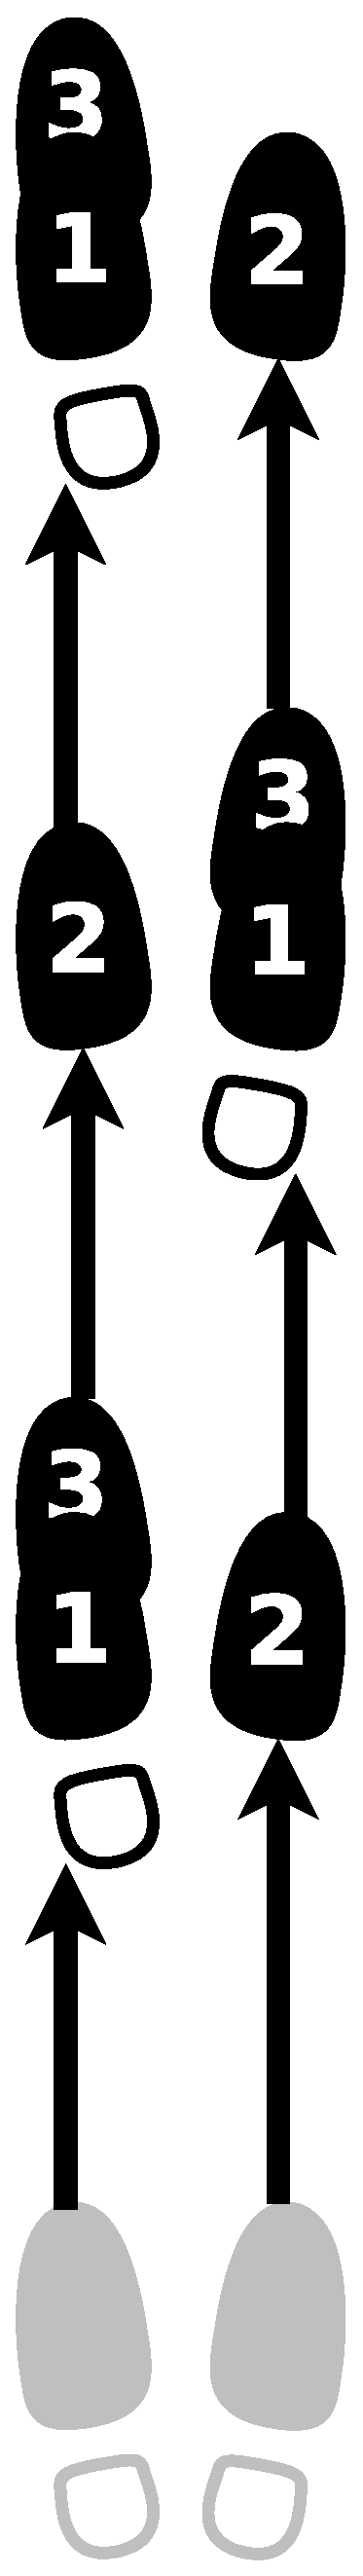
\includegraphics[width=0.25\textwidth]{chapters/cap-historia-sambagafieira/samba-batucada-basico-frente.eps}
        \caption{Passo básico para a frente.}
        \label{fig:samba-batucada-basico-frente}
    \end{subfigure}
    ~ %add desired spacing between images, e. g. ~, \quad, \qquad, \hfill etc. 
      %(or a blank line to force the subfigure onto a new line)
    \begin{subfigure}[b]{0.4\textwidth}
        \centering
	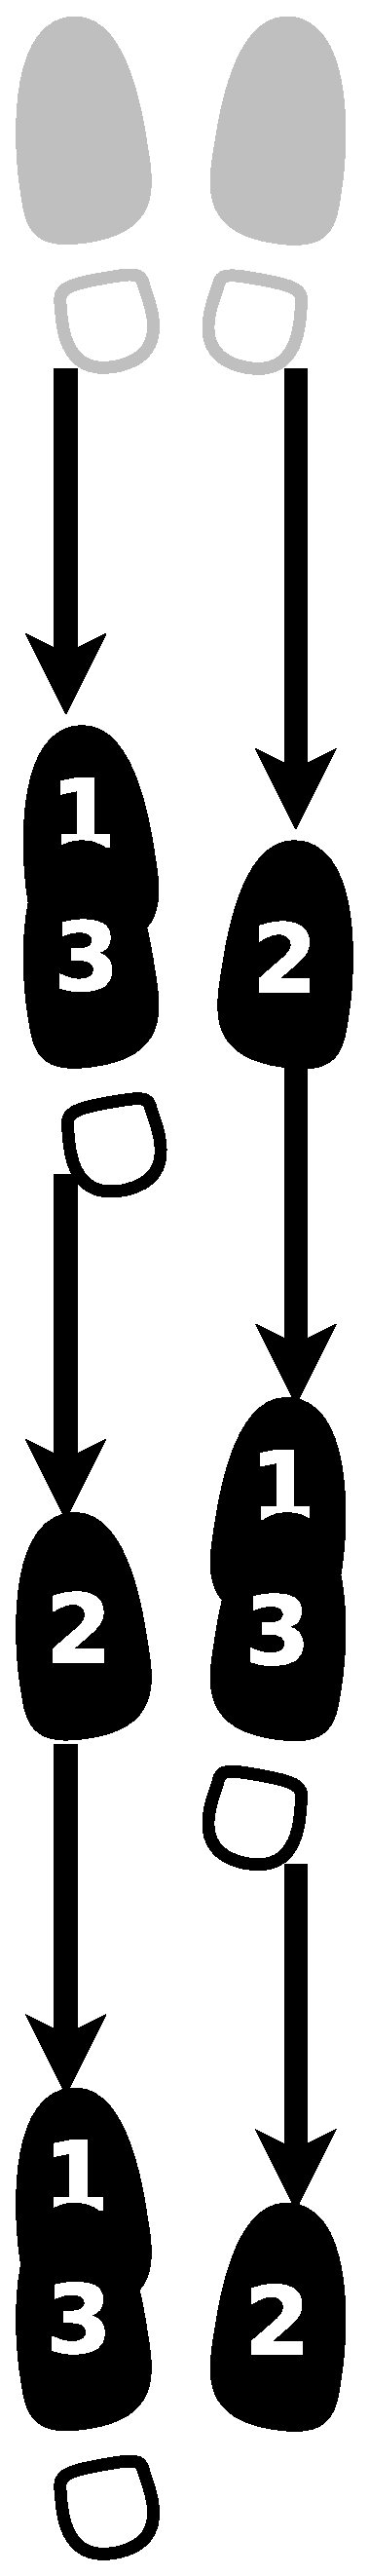
\includegraphics[width=0.25\textwidth]{chapters/cap-historia-sambagafieira/samba-batucada-basico-tras.eps}
        \caption{Passo básico para trás.}
        \label{fig:samba-batucada-basico-tras}
    \end{subfigure}
    \caption{Samba-batucada da década de 1959.}\label{fig:samba-batucada-basico}
\end{figure}

Outros passos conhecidos no ano de 1947, para este estilo de samba, tem nomes como: 
o pião, o balão, a cortada, a meia cortada, a joelhada, a patineta, e outros \cite[pp. 66]{fornaciari1947aprender};
porem, seguindo o Prof. Fornaciari, o pião e o balão são o mesmo movimento, 
sendo este o movimento mais importante do samba-batucada;
e a diferença do pião atual que se executa tradicionalmente em sentido horário,
o pião de 1947 se executava em sentido anti-horário \cite[pp. 68,72]{fornaciari1947aprender}.




\item \textbf{Samba liso}, 
\index{Dança!Samba liso}
Era uma dança com balanços que se dançava sem flexionar os joelhos;
este é um estilo de dança que perdura ainda ate nossos 
dias \cite[pp. 58,62]{freitas1959danca} \cite[pp. 143]{perna2002samba}, 
para mais detalhes ver a Seção \ref{subsec:estilosdedancapares}.
\end{itemize}

\subsection{Evolução do samba nos salões}

Com o passar dos anos foram agregados elementos de outras danças a esse primitivo, samba de gafieira;
por exemplo, movimentos do tango e do rock \cite[pp. 142]{perna2002samba}, 
obtendo assim a forma de dança que vemos hoje em dia, ver Figura \ref{fig:formuladosambagafieira2}.

Asim, podemos falar do samba de gafieira como dança, só apos da aparição do samba nos
salões de dança abertos ao público, e a partir da criação do termo gafieira pra definir a estes lugares.
Com a mistura destes dois acontecimentos obtemos o termo, samba de gafieira,
que iniciou seu caminho na dança, mas como uma descrição do âmbito da dança (e da música), que como nome próprio.
Porem, a formação dos movimentos e corporalidade desta dança tem um caminho que data desde muito tempo atrás,
desde os batuques, dos morros e das rodas.


A primeira referencia achada\footnote{Que não quer dizer a primeira existente.} 
na ``Hemeroteca Digital Brasileira'' da Fundação Biblioteca Nacional,
foi na ``Revista da Semana''(RJ), no dia 25 de dezembro de 1948,
onde na seção ``Eros Volusia'', subseção ``O pitoresco da excursão'', se indica \cite[pp. 48]{sambagafieirarefbn}
\begin{citando}
Ensinando o samba aos ministros da República, 
fazendo o povo vibrar com o \textbf{samba de gafieira}, entusiasmando
o meio intelectual com seu francês muito doce,
contando coisas desconhecidas aos dançarinos francêses,
fazendo a dança brasileira figurar nos Archives Internationales de la Danse.
Eros Volusia satisfez o grande ideal de sua vida artística, sentindo-se contente
com o que realizou na França, embora a Europa não dê dinheiro a ninguém.
O lucro artístico é que compensa.
\end{citando}


A Figura \ref{fig:sambagafieiracrono} mostra a cronologia do uso do termo samba de gafieira. 

\begin{figure}[h]
  \centering
    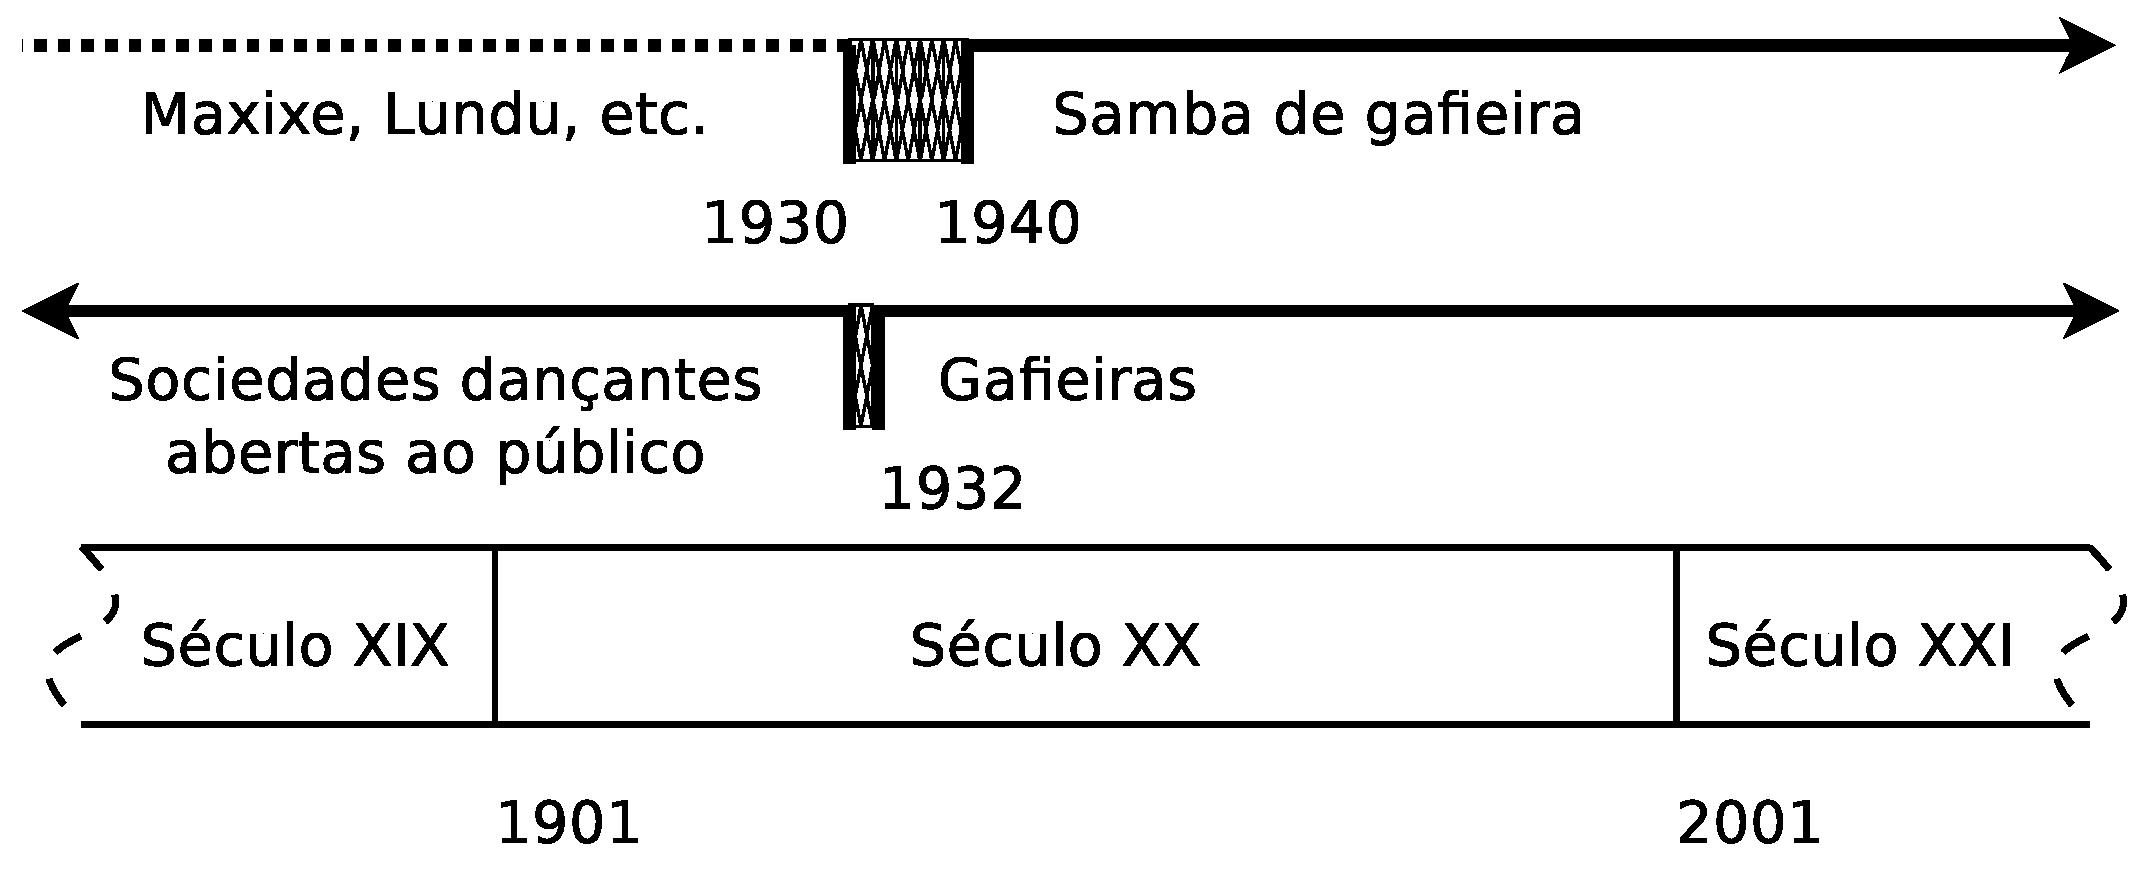
\includegraphics[width=1.0\textwidth]{chapters/cap-historia-sambagafieira/gafieira-crono.eps}
  \caption{ Cronologia da formação do samba de gafieira.}
\label{fig:sambagafieiracrono}
\end{figure}

%%%%%%%%%%%%%%%%%%%%%%%%%%%%%%%%%%%%%%%%%%%%%%%%%%%%%%%%%%%%%%%%%%%%%%%%%%%%%%%
%\clearpage
\section{Música para dançar samba de gafieira}
\label{subsec:gafieiradancaestilos}

Entre os estilos musicais em que o samba de gafieira (dança) se adapta bem, 
estão alguns dos subgêneros do samba; assim,
aqui mencionaremos uma lista de músicas que por sua graça, estilo e alegria,
a meu entender, podem ser dançados usando o samba de gafieira. Porem, 
estas músicas não pretendem ser máximos expoentes representativos, do subgênero em que estão agrupados;
e sim uma indicação ou orientação ao leitor, 
para treinar sua dança usando músicas em que possa ser mais confortável a experiencia.

\begin{itemize}
\item \textbf{Samba de gafieira (música)}
\begin{example} ~
\begin{itemize}
%\item ``Samba de padua'' interpretado pelo grupo Turma da Gafieira.
\item ``Samba de morro'' interpretado pelo grupo Turma da Gafieira.
%\item ``Piston da gafieira'' de Billy Blanco, interpretado por Jorge Beiga.
\item ``Piston da gafieira'' de Billy Blanco, interpretado por Zeca pagodinho \cite{barbosa2014zeca}.
\item ``Beija-me'' de Roberto Martins e Mário Rossi, interpretado por Zeca pagodinho \cite{barbosa2014zeca}.
\item ``Pisei num despacho'' de Geraldo Pereira e Elpídio Viana, interpretado por Zeca pagodinho \cite{barbosa2014zeca}.
%\item ``Tive sim'' de Cartola, interpretado por Zeca pagodinho \cite{barbosa2014zeca}.
%\item ``Tarzan, o filho do alfaiate'' de Noel Rosa e Vadico, interpretado por Zeca pagodinho \cite{barbosa2014zeca}.
%\item ``Se você visse'' de Dino 7 cordas e Del Loro, interpretado por Zeca pagodinho \cite{barbosa2014zeca}.
\end{itemize}
\end{example} 

\item \textbf{Samba de breque}
\begin{example} ~
\begin{itemize}
\item ``Baile no elite'' interpretado por Casuarina.
\item ``Eu sou a marrom'' interpretado por Alicione.
%\item ``Hoje sou diferente'' interpretado por Lenita Rodrigues.
\item ``Pra levantar poeira'' interpretado por Bodhar.
\end{itemize}
\end{example} 

\item \textbf{Pagode paulista (Sambalanço)}
\begin{example} ~
\begin{itemize}
\item ``Cheia de manias''  interpretado pelo grupo Raça Negra.
\end{itemize}
\end{example} 

\item \textbf{Partido alto}
\begin{example} ~
\begin{itemize}
%\item ``A língua'' interpretado por Beto lima.
\item ``Partido Alto'' interpretado por Aleh.
\end{itemize}
\end{example} 

\item \textbf{Pagode}
\begin{example} ~
\begin{itemize}
\item ``Trilha Do Amor''  interpretado pelo Grupo Revelação. 
\item ``A Batucada Te Pegou'' interpretado pelo Grupo Sou Muleke.
\item ``Dança da Solidão'' interpretado por Pagode de Mesa do álbum Terra Brasil. 
\item ``Eu e você sempre'' interpretado por Jorge Aragão
\end{itemize}
\end{example} 

\item \textbf{Samba-canção (música)}
\begin{example} ~
\begin{itemize}
\item ``Eu Quero E Sossego'' interpretado por Paulo Moura.
\item ``Só Louco'' interpretado por Luiz Melodia.
\item ``Você É a Fonte'' interpretado por  Quinteto em Branco e Preto.
\item ``Eu Quero é Sossego'' interpretado por Paulo Moura.
\end{itemize}
\end{example} 

\item \textbf{Bossa nova}
\begin{example} ~
\begin{itemize}
\item ``I Don't Know (Bossa Mix)'' interpretado por Erika do álbum ``I Don't Know''
\item ``Human Nature'' interpretado por Marcela Mangabeira.
\end{itemize}
\end{example} 


\item \textbf{Choro}
\begin{example} ~
\begin{itemize}
\item ``Choro de gafieira'' de Pixinguinha.
\item ``Chorinho de gafieira'' de Astor Silva.
\item ``Noites Cariocas'' de Jacob do Bandolim.
\end{itemize}
\end{example} 


\item \textbf{Samba-choro}
\begin{example} ~
\begin{itemize}
\item ``Escurinho'' interpretado por Corina Magalhães.
\item ``Tico Tico no Fubá'' interpretado por Leci Brandão.
\end{itemize}
\end{example}

\end{itemize}

A Figura \ref{fig:gafieiradancaestilos} mostra um resumo de alguns dos 
subgêneros do samba onde pode ser dançado o samba de gafieira.
\begin{figure}[h]
  \centering
    \includegraphics[width=0.7\textwidth]{chapters/cap-historia-sambagafieira/gafieiravcmusica.eps}
  \caption{ Subgêneros do samba onde pode-se dançar samba de gafieira.}
\label{fig:gafieiradancaestilos}
\end{figure}




\part{O samba e a dança de salão}
%%%%%%%%%%%%%%%%%%%%%%%%%%%%%%%%%%%%%%%%%%%%%%%%%%%%%%%%%%%%%%%%%%%%%%%%%%%%%%%%
%% Capitulo
%%%%%%%%%%%%%%%%%%%%%%%%%%%%%%%%%%%%%%%%%%%%%%%%%%%%%%%%%%%%%%%%%%%%%%%%%%%%%%%%
\chapterimage{chapter_head_2.pdf} % Chapter heading image

\chapter{Estilos de dança no samba}

%%%%%%%%%%%%%%%%%%%%%%%%%%%%%%%%%%%%%%%%%%%%%%%%%%%%%%%%%%%%%%%%%%%%%%%%%%%%%%%%
%%%%%%%%%%%%%%%%%%%%%%%%%%%%%%%%%%%%%%%%%%%%%%%%%%%%%%%%%%%%%%%%%%%%%%%%%%%%%%%%
\section{Que estilo de dança posso usar no samba (música)?}
\label{subsec:estilosdedanca}
A resposta mais simples poderia ser que, uma pessoa ao ser livre e independente,
pode escolher expressar-se na dança, de forma natural, como esta saia de si mesmo.
Porém, entrando em assuntos mais técnicos, 
e de acordo com os padrões socialmente mais comuns de ser achados atualmente;
existe um grupo de modalidades de dança, que por suas caraterísticas, 
são consideradas que se enquadram muito bem na música de alguns subgêneros do samba.

Assim, nas seguintes seções, serão descritos alguns dos estilos de dança para a música do samba,  
que podemos achar nos salões e locais de dança no Brasil;
estes serão agrupados em estilos \textbf{dançados em pares}, e os que são \textbf{dançados de forma separada}. 


%%%%%%%%%%%%%%%%%%%%%%%%%%%%%%%%%%%%%%%%%%%%%%%%%%%%%%%%%%%%%%%%%%%%%%%%%%%%%%%%
\section{Estilos dançados em pares}
\label{subsec:estilosdedancapares}
Entre os estilos que se dançam a dois no samba, no ano \AnoLivro, temos \cite[pp. 134]{perna2002samba}:

%%%%%%%%%%%%%%%%%%%%%%%%%%%%%%%%%%%%%%%%%%%%%%%%%%%%%%%%%%%%%%%%%%%%%%%%%%%%%%%%
\subsection{Samba de gafieira (dança)} 
\index{Dança!Samba de gafieira}
É uma dança a dois que pode ser executada na maioria dos subgêneros do samba (música),
tendo exceções em: samba-enredo, samba reggae (música), samba rock (música), 
marcha, marcha-rancho e maxixe (música);
nos seus origens este tipo de dança era chamado de samba-batucada  \cite[pp. 134]{perna2002samba}, 
mais detalhes do samba de gafieira no Capítulo \ref{cap:sambagafieira}.

%%%%%%%%%%%%%%%%%%%%%%%%%%%%%%%%%%%%%%%%%%%%%%%%%%%%%%%%%%%%%%%%%%%%%%%%%%%%%%%%
\subsection{Samba liso} 
\label{subsec:sambalisodef}
\index{Dança!Samba liso}
%\index{Dança!Samba caminhado}
Atualmente se dança similarmente ao samba de gafieira, 
porém com um estilo mais elegante, sem ginga né passos de efeito, e dizer é uma dança mais ``lisa'';
se dança bem em: samba-canção, bossa nova e choro \cite[pp. 134]{perna2002samba}.

\PRLsep{Referencias ao samba liso (1917-1933):} 

Podemos achar uma referencia interessante ao uso do termo \textbf{samba} e \textbf{liso}  no livro 
``Feitiço decente: Transformações do samba no Rio de Janeiro (1917-1933)'' (2001),
na qual se pode intuir a procedência deste nome ou denominação, 
quando se faz referencia a um comentário de João da Baiana sobre o samba-de-umbigada e o samba de roda \cite[pp. 109]{sandroni2001feitico}: 
\begin{citando}
Nós tirávamos um verso e o pessoal sambava, um de cada vez ... 
Um saía para tirar o outro.
Se fosse a ``liso'' era só umbigada, mas se fosse para pegar ``duro'' já era capoiragem. 
\end{citando}
Assim, no livro se comenta que existiam duas modalidades para que o dançarino solista escolha a seu sucessor, 
dependendo do tipo de roda, em ``samba liso'' (com umbigada) ou em ``samba duro'' 
(ou batucada\footnote{No qual a umbigada é substituída por uma pernada \cite[pp. 109]{sandroni2001feitico},
para mais detalhes ir a página \pageref{ref:batuquedanca}.}) \cite[pp. 109]{sandroni2001feitico}.
Esta referencia 
é particularmente interessante, pois como veremos na Seção \ref{cap:sambagafieira},
nos primórdios do samba, nas gafieiras existiam 3 modalidades em que o samba era dançado: samba-canção (dança),
\textbf{samba-batucada} (dança)\footnote{Este 
é o nome com o qual era conhecido originalmente o atual samba de gafieira \cite[pp. 143]{perna2002samba}.} 
e \textbf{samba-liso} \cite[pp. 143]{perna2002samba};
estas duas últimas, não são as mesmas danças do samba-de-umbigada, 
e sim novas formas de dançar o samba num ambiente mais civilizado como o salão de dança;
porém, estes nomes conservavam a mesma nomenclatura, na descrição 
relativa à tosquedade dos movimentos, entre uma dança mais suave ou lisa, 
e outra dura ou batucada.

%%%%%%%%%%%%%%%%%%%%%%%%%%%%%%%
\PRLsep{Referencias ao samba liso (1950-1953)}


Na ``Hemeroteca Digital Brasileira'' da Fundação Biblioteca Nacional,
não tem-se achado referencias\footnote{ Foram achadas,
2, 5, 3, 1 e 1 referencias brutas para as décadas de 1930, 1940, 1960, 1970 e 1980 respetivamente;
porém, estas não eram relativas ao samba liso de salão ou eram falsos acertos.} 
à frase ``\textbf{samba liso}'', nas décadas de 1930, 1940, 1960, 1970 e 1980;
as referencias achadas correspondem à década de 1950\footnote{Especificamente entre os anos 1950 e 1953.}  
com uma total de 327 referencias;
de todas estas, 326 correspondem à forte campanha 
de marketing do livro
``Como aprender a dançar'', 
de Gino Forniciari. 
Por exemplo, podemos achar a primeira referencia em ``O Jornal'' (RJ),
do dia 17 de setembro de 1950, no qual pode-se ler \cite[3ra seção pp. 9]{jornalanunciodanca1}:
\begin{citando}
\begin{center}
Como aprender a dançar\\
4a edição ampliada
\end{center}
Com a nova dança, ``Baião'', \textbf{Samba liso}, e os
últimos passos de Bolero, Rumba, Swing, contendo
120 gráficos 330 passos, facilitando as senhoritas 
e cavalheiros a aprenderem em suas próprias 
casas em 10 dias apenas, no princípio sem
companheiro ou companheira. Método de ritmos modernos
pelo Prof. Gino Fornaciari, 
Diretor e Prof. do ``CURSO PRATICO DE DANÇAS RITZ''.
Aulas particulares, rua da Liberdade, 120.
Preço: Cr\$ 45,00 -- Pedidos pelo reembolso posta 
-- com o autor -- Caixa Postal, 649 -- SÃO PAULO 
\end{citando}
Todos estes anúncios vem na maioria das vesses acompanhados com um desenho como
o mostrado na Figura \ref{fig:desenholivrodanca1}, o qual indica todos os estilos de dança abordados no livro;
fazendo uma diferencia entre dançar \textbf{samba} e \textbf{samba liso}.
\begin{figure}[h]
  \centering
    \includegraphics[width=0.6\textwidth]{chapters/cap-historia-dancasamba/comoaprenderdancar.jpg}
  \caption{Desenho da publicidade do livro ``Como aprender a dançar'' de Gino Forniciari,
publicado, no dia 17 de fevereiro de 1952, em ``Sport Ilustrado'' \cite[pp. 22]{sportlivropublidanca}.}
\label{fig:desenholivrodanca1}
\end{figure}
Ja no decorrer do livro o autor, define o samba de salão e apresenta 3 modalidades,
de ser dançado, sendo uma destas o samba liso \cite[pp. 61]{fornaciari1950aprender}.
É interessante ressaltar que na segunda edição deste livro, lançada no ano de 1947,
não tinha nenhuma referencia ao samba liso, ficando a incógnita se esta omissão era
porque a modalidade nessa época era pouco conhecida e recente, ou por desconhecimento do autor.



%%%%%%%%%%%%%%%%%%%%%%%%%%%%%%%
A outra referencia achada na ``Hemeroteca Digital Brasileira'' da Fundação Biblioteca Nacional,
com a frase ``samba liso'', na década de 1950, foi a publicada o dia 26 de agosto de 1951,
no ``Diário do Nordeste'' de Caixas do Sul (RS), numa cronica de Walter Brugger da sua viagem por Europa,
num articulo titulado ``Genova! Primeiro Contato com a Europa!'',
no qual pode-se ler \cite[pp. 10]{nordestesambalisocronica}:
\begin{citando}
Ao nosso lado, numa área 
descoberta uma orquestra tocava para
quem quizesse dançar.
Repentinamente ouvimos uma melodia muito
nossa conhecida. Era o imortal ``Tico-Tico no Fubá''... Todavia,
apesar da melodia correta, o ritmo
era bastante falho. Continuando 
com os ritmos brasileiros, a orquestra 
tocou ainda ``Chiquita Bacana'',
mas em tempo de samba e ``Aquarela do Brasil''.
O que porém nos 
deixou mais atônitos foi o modo como 
era dançado o nosso samba. De 
brasileiro não tinha nada. Pelo que 
vimos, o \textbf{samba ``liso''} lhes é desconhecido 
e cada um procura ``requebrar'' o corpo mais que o outro,
mas de uma forma como nós só 
conhecemos no cinema mexicano. 
O meu amigo dava gostosas risadas e não era para menos,
ante a comicidade do espetáculo, tão 
impossível no Brasil quanto desconhecido para nós.
\end{citando}


%%%%%%%%%%%%%%%%%%%%%%%%%%%%%%%
\PRLsep{Referencias ao samba liso (1955)}

Outra referencia ao \textbf{samba liso}, pode ser achada no livro ``Manual de Danças Gaúchas'' (1955)
no qual se afirma que \cite[pp. 77]{cortesmanual}: 
\begin{citando}
A polquinha, como dança especifica, é executada por pares enlaçados,
mediante passos-de-marcha (É correograficamente  semelhante ao chamado 
\textbf{samba liso} ou \textbf{samba caminhado} dos salões urbanos).
\end{citando}~\\

%%%%%%%%%%%%%%%%%%%%%%%%%%%%%%%
\PRLsep{Descrição do samba liso (1959)}

Era uma dança na qual se bamboleia o corpo e se dançava sem flexionar os joelhos \cite[pp. 58]{freitas1959danca} \cite[pp. 143]{perna2002samba},
era dançado usando 4 movimentos (em 2 compassos) \cite[pp. 62]{freitas1959danca} \cite[pp. 143]{perna2002samba}.
Sobre os passos usados nessa época, 
na Figura \ref{fig:samba-liso-basico-frente} se mostra o passo básico para a frente do samba liso,
e na  Figura \ref{fig:samba-liso-basico-frente} o mesmo movimento para trás; 
em ambos casos se usam os 4 movimentos antes mencionados, e a cor cinza indica a posição inicial \cite[pp. 63]{freitas1959danca}. 
\begin{figure}[h]
    \centering
    \begin{subfigure}[b]{0.4\textwidth}
        \centering
        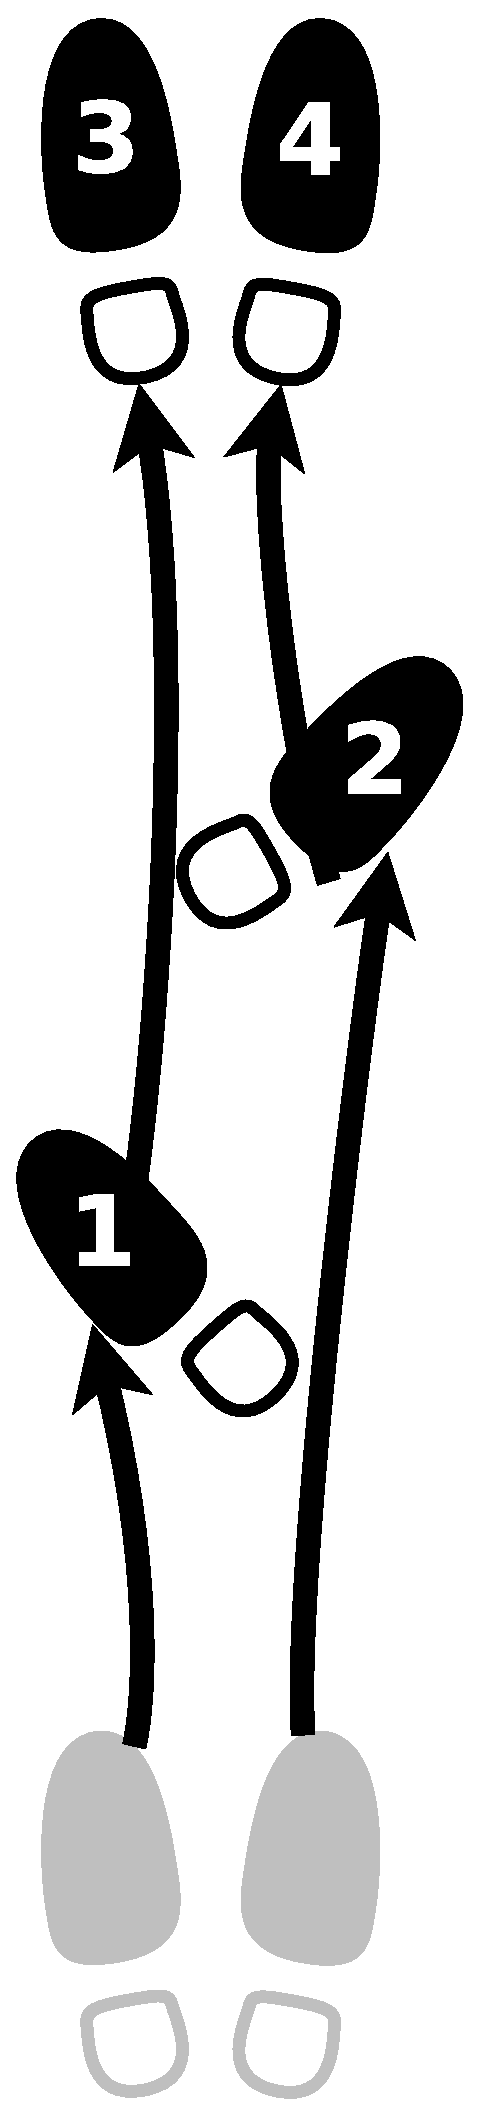
\includegraphics[width=0.25\textwidth]{chapters/cap-historia-dancasamba/samba-liso-basico-frente.eps}
        \caption{Passo básico para a frente.}
        \label{fig:samba-liso-basico-frente}
    \end{subfigure}
    ~ %add desired spacing between images, e. g. ~, \quad, \qquad, \hfill etc. 
      %(or a blank line to force the subfigure onto a new line)
    \begin{subfigure}[b]{0.4\textwidth}
        \centering
	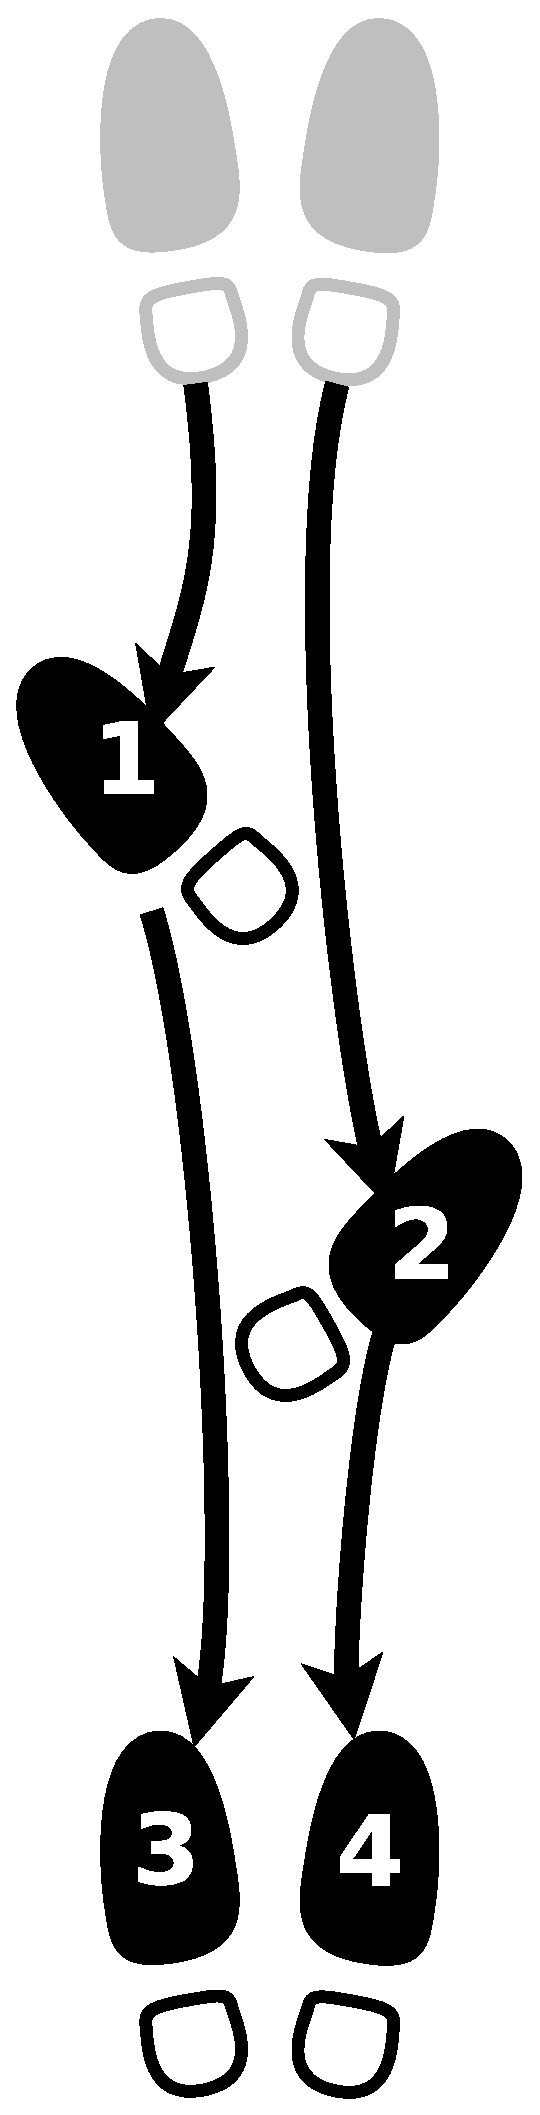
\includegraphics[width=0.25\textwidth]{chapters/cap-historia-dancasamba/samba-liso-basico-tras.eps}
        \caption{Passo básico para trás.}
        \label{fig:samba-liso-basico-tras}
    \end{subfigure}
    \caption{Samba liso da década de 1950.}\label{fig:samba-liso-basico}
\end{figure}

%%%%%%%%%%%%%%%%%%%%%%%%%%%%%%%%%%%%%%%%%%%%%%%%%%%%%%%%%%%%%%%%%%%%%%%%%%%%%%%%
\subsection{Samba pagode} 
\index{Dança!Samba pagode}
É um estilo de dança a dois, originário de São Paulo, 
sendo esta uma dança com poucos deslocamentos \cite[pp. 134]{perna2002samba}.
É um estilo de dança adaptado para ser dançado com o pagode paulista,
também chamado como Sambalanço em 1990.
%% https://www.youtube.com/watch?v=SfvoiXOGPn4
De forma similar ao pagode que teve duas épocas com estilos musicais diferentes\footnote{Ver página \pageref{ref:sambalanco}.}
(samba raiz e sambalanço),
a dança samba pagode, sofreu também transformações acompanhando essas tendencias.
Podem-se observar, no ano \AnoLivro, 3 tipos de passo básico: 
%% https://www.youtube.com/watch?v=rq1uhNXySds 
%% https://www.youtube.com/watch?v=SfvoiXOGPn4

O miudinho, que é um passo que se realiza abraçado com o par de dança e de forma espelhada entre eles,
no qual se executam 3 twist\footnote{É importante ter um sapato que deslise bem.} no lugar, 
só trocando de peso entre os pés, seguindo um ritmo rápido-rápido lento.
Este movimento se executa simetricamente duas vesses para formar um ciclo completo.  
Se uma vez se inicia com o peso do corpo no pé direito\footnote{Quando o primeiro twist é horário.} 
então na próxima vez se inicia com o pé esquerdo.

O passo básico lateral se realiza abraçado com o par de dança e de forma espelhada com este, 
é similar ao passo básico de capoeira,
ou a base aberta do forró\footnote{Só que aqui é abraçados.},
no qual se produzem 3 movimentos seguindo um ritmo rápido-rápido lento,
no primeiro momento, um pé vai para atrás, 
no segundo o outro pé ajeita sua posição deslocando-se levemente, 
procurando o centro e o equilíbrio do par dançante,
no terceiro movimento o pé que estava atrás volta ao lado do outro pé.
Este movimento se executa simetricamente duas vesses para formar um ciclo completo,  
uma vez se inicia com pé direito e o seguinte com o pé esquerdo.
Este movimento é interessante para fazer deslocamentos, 
os quais são realizados principalmente no primeiro movimento com o pé para trás, 
só que agora apontando para uma direção escolhida por nós.

A caidinha, se realiza abraçado com o par, 
este passo é similar ao picadilho (picadinho) de samba de gafieira,
porém com um deslocamento similar ao repique do forró;
no pagode paulista este movimento se executa seguindo um ritmo, rápido-rápido lento,
no qual o seguidor faz um movimento similar ao miudinho antes mencionado,
enquanto que o condutor tem uma liberdade criativa no 
seu movimento\footnote{O mesmo que acontece no picadilho de samba de gafieira.},  
respeitando-se sempre o ritmo rápido-rápido lento.

%%%%%%%%%%%%%%%%%%%%%%%%%%%%%%%%%%%%%%%%%%%%%%%%%%%%%%%%%%%%%%%%%%%%%%%%%%%%%%%%
\subsection{Samba rock (dança)}
\index{Dança!Samba rock}
É um estilo de dança a dois, realizado nos bailes ``black'' paulistas desde a década de 1960, 
sendo esta uma dança variante das danças do swing/rock e parente do soltinho carioca \cite[pp. 135]{perna2002samba}.
Se dança bem em músicas: Swing, samba rock (música), samba com suingue e samba-funk \cite[pp. 135,138]{perna2002samba}.
O samba rock se dança de mão dadas, e se carateriza por ter muitas voltas,
executadas na maior parte de vesses pelos seguidores.
Esta é uma dança estacionaria pois os dançantes rara vez se deslocam no salão, 
em geral eles ficam trabalhando seus passos num mesmo lugar  \cite[pp. 135,138]{perna2002samba}.
Quando um espectador externo vê esta dança perceberá muitas figuras usando predominantemente os braços,
com enrosques, voltas, enlaces, entre outros,
enquanto os pés de ambos dançarinos fazem uma mesma marcação, num constante e cíclico rápido-rápido lento,
caminhando sobre um circulo imaginário no chão, uma vez em sentido horário e outra em anti-horário.

%%%%%%%%%%%%%%%%%%%%%%%%%%%%%%%%%%%%%%%%%%%%%%%%%%%%%%%%%%%%%%%%%%%%%%%%%%%%%%%%
\subsection{Samba funkeado}
\label{subsec:sambafunkeado}
\index{Dança!Samba funkeado}
Também é chamado de estilo Jimmy de Oliveira ou simplesmente  samba Jimmy, 
em aluição a seu criador.
Este estilo de dança a dois foi criado no ano de 1998.
Com muito esforço Jimmy, num período aproximado de 6 meses, 
criou a estrutura da dança, desde iniciante ate avançado;
no ano de 1999 ele  chamou a esse estilo como ``samba quebrado'';  
posteriormente renomeou  para ``samba Jimmy'', 
recebeu algumas criticas e no ano 2001 decidiu renomeá-lo para ``samba funk'',
porém isto trouxe confusões   ao ser associado com a música funk, existente em Rio de Janeiro,
a qual era muito distante da proposta dele, e
finalmente a meados do 2005 ele decidiu chamá-lo ``samba funkeado''  \cite{sambafunkeadoJimmyDeOliveiraPart1}.
A Figura \ref{fig:funkeadocrono1} mostra a cronologia de nomes para este estilo.
\begin{figure}[h]
  \centering
    \includegraphics[width=1.0\textwidth]{chapters/cap-historia-dancasamba/sambafunkeado.eps}
  \caption{Cronologia dos nomes para samba funkeado.}
\label{fig:funkeadocrono1}
\end{figure}

Em palavras de Jimmy de Oliveira o estilo foi criado para: ``contribuir em função da música'', 
numa tentativa de agregar movimento em coerência como as músicas que ele gostava;
sendo estas interpretadas por:
Djavan, Jorge Ben Jor, Tim Maia, Leny Andrade \cite{sambafunkeadoJimmyDeOliveiraPart1}, que em seu momento, 
presentaram músicas de bossa nova ou que eram influenciadas pelo jazz, 
funk norte-americano ou ``black music'' \cite{sambafunkeadoJimmyDeOliveiraPart1} \cite{sambafunkeadoJimmyDeOliveiraPart3},
Jimmy indica que seu estilo procura ir em função da música escutada no brasil, 
e que a maioria da música atual é influenciada pelo funk norte-americano;
como a música de: João Sabiá. 

 
Seguindo a professora de dança Erika Ikuno, no 2003, 
mediante o lançamento do album ``A procura da batida perfeita'' do rapper Marcelo D2,
se presentou um trabalho musical brasileiro relativo ao samba que aos olhos de Jimmy e ela
envolvia todo o que procuravam musicalmente quando dançavam samba funkeado,
de modo que a partir de então a maioria dos dançarinos inciaram a preferir gêneros 
musicais brasileiros (samba com hiphop) para dançar samba funkeado \cite[pp. 92]{filho2016tango},
pois até então a tendencia era escolher gêneros musicais estrangeiros.

O samba funkeado pode ser dançado em gêneros como ``black music'',
em pagodes funkeados (Sorriso maroto, Netinho de Paula, pixote, etc.), 
em sambas com influencia do jazz \cite{sambafunkeadoJimmyDeOliveiraPart3}, etc.

O samba funkeado tem 3 tendencias ou estruturas  \cite{sambafunkeadoJimmyDeOliveiraPart2}:
\begin{itemize}
\item \textbf{Samba funkeado}, primigênio.
\item \textbf{Samba funkeado fragmentado}; exemplo: um movimento que é de sentar, que gastaria um tempo, 
passa a ter ate 3 tempos; é dizer, fragmenta os movimentos. 
O fragmentado também permite dançar com movimentações em contrapeso no par de dança.
\item \textbf{Samba funkeado samsurf}, com uma postura mais curvada.
\end{itemize}

%e em seu ídolo Michael Jackson \cite{sambafunkeadoJimmyDeOliveira2}.
 
%%%%%%%%%%%%%%%%%%%%%%%%%%%%%%%%%%%%%%%%%%%%%%%%%%%%%%%%%%%%%%%%%%%%%%%%%%%%%%%%
\subsection{Samba internacional}
\label{subsec:DancaSambaInternacional} 
\index{Dança!Samba internacional}
É um estilo de dança a dois, influenciado pelo maxixe;
se dança principalmente fora do Brasil e existem basicamente dois estilos: 
o estilo internacional e o estilo norte-americano (EE.UU.) \cite[pp. 134-135]{perna2002samba}.

O samba introduzido a EE.UU. é uma dança de salão muito animada, 
com música de ritmo alegre, que sugere um estilo de movimento que pode
chegar a ser tão turbulento quanto os movimentos do Jive.
O padrão de passos básicos é similar aos achados no Fox-Trot e o Waltz;
%sendo estes: fwd-swd-close ... bwd-swd-close; e
com uma distribuição de tempos que segue uma sequência: 
quick-quick-slow\footnote{Rápido-rápido-lento.} ... quick-quick-slow \cite{parson2016ballroom}.

Observando os campeonatos internacionais nos quais este estilo é usado, 
se percebe que o samba internacional é dançado em qualquer estilo musical que
tenha sotaque ou de a impressão de ter raiz afro-latina.

%%%%%%%%%%%%%%%%%%%%%%%%%%%%%%%%%%%%%%%%%%%%%%%%%%%%%%%%%%%%%%%%%%%%%%%%%%%%%%%%
\subsection{Relações entre os subgêneros do samba e os estilos dançados em pares}

A Figura \ref{fig:sambadavavsmusica} mostra as relações entre os estilos de dança a dois (na esquerda),
 e alguns subgêneros musicais do samba (na direita) \cite[pp. 134-138]{perna2002samba}.

\begin{figure}[h]
  \centering
    \includegraphics[width=1.0\textwidth]{chapters/cap-historia-dancasamba/dancavcmusica.eps}
  \caption{Relações entre os estilos de dança a dois e os subgêneros do samba.}
\label{fig:sambadavavsmusica}
\end{figure}

%%%%%%%%%%%%%%%%%%%%%%%%%%%%%%%%%%%%%%%%%%%%%%%%%%%%%%%%%%%%%%%%%%%%%%%%%%%%%%%%
%%%%%%%%%%%%%%%%%%%%%%%%%%%%%%%%%%%%%%%%%%%%%%%%%%%%%%%%%%%%%%%%%%%%%%%%%%%%%%%%
\section{Estilos dançados de forma separada}
No ano \AnoLivro~podemos observar os seguintes estilos \cite[pp. 134]{perna2002samba}:

\subsection{Samba reggae  (dança)} 
Este estilo de samba se dança de forma separada, 
é uma dança baiana também conhecida como axé-dance, samba baiano ou pagode baiano,
se dança em músicas de samba reggae \cite[pp. 134]{perna2002samba}.

\subsection{Samba no pé} 
É o estilo usado nas quadras das escolas de samba,
se dança bem em estilos musicais como: 
samba enredo ou em qualquer samba rápido  \cite[pp. 134]{perna2002samba}.

\subsection{Marcha de carnaval}
 É uma dança própria do carnaval para se dançar em cordões.
se dança bem em: marchas, marchas-rancho e samba-enredo lentos  \cite[pp. 135]{perna2002samba}.


\subsection{Relações entre os subgêneros do samba e os estilos dançados de forma separada}

A Figura \ref{fig:sambadavavsmusicaseparado} mostra as relações existentes, 
entre os estilos de dança no samba que se dançam de forma separada (na esquerda) 
e alguns subgêneros musicais do samba (na direita)  \cite[pp. 134-138]{perna2002samba}.

\begin{figure}[h]
  \centering
    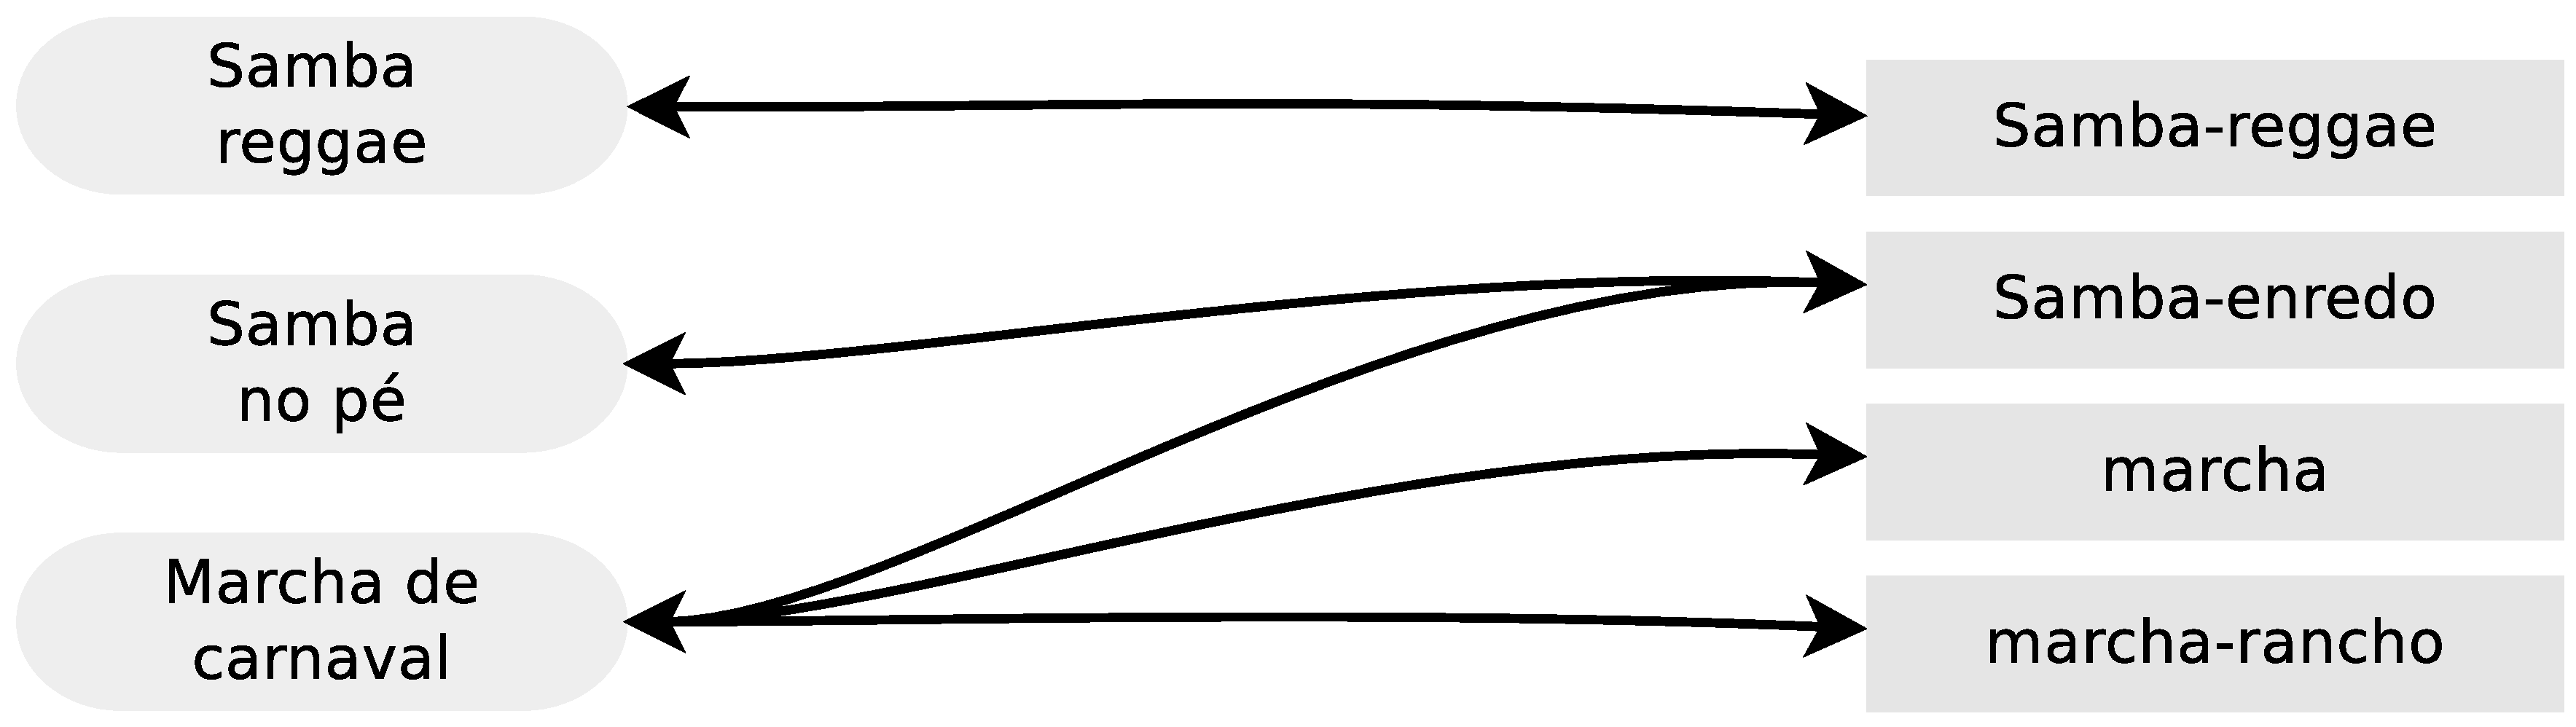
\includegraphics[width=1.0\textwidth]{chapters/cap-historia-dancasamba/dancavcmusicaseparado.eps}
  \caption{Relações entre os estilos de dança (separados) e os subgêneros do samba.}
\label{fig:sambadavavsmusicaseparado}
\end{figure}

\chapterimage{chapter_head_2.pdf} % Chapter heading image

\chapter{Regras na dança de salão}

Antes de iniciar as explicações no capítulo, 
é necessário partir desde uma linguagem comum;
com este propósito, 
significados de algumas palavras bem definidas na literatura são mostrados a continuação:
 
\begin{definition}[Regra:] 
\index{Regras}
\label{def:Regra}
Princípio que serve como padrão no estudo das artes e ciências \cite{priberamregra} \cite{dicioregra}.
Exemplo: regras gramaticais; regras de etiqueta; regras do jogo; regras na dança.
\end{definition}

\begin{definition}[Casal:] 
\index{Casal}
\label{def:Casal} O Dicionário Priberam da Língua Portuguesa \cite{priberamcasal} define casal como:
Par formado por um macho e uma fêmea.
Exemplo: casal de cavalos, casal de pombas, casal de humanos.
\end{definition}

\begin{definition}[Par:] 
\index{Par}
\label{def:Par} O Dicionário Priberam da Língua Portuguesa \cite{priberampar} define par como:
Igual, semelhante, parceiro.
Cada uma das pessoas que constituem uma dupla na dança.
\end{definition}


Usando como base os significados mostrados anteriormente, 
serão descritos alguns termos muito utilizados na dança\footnote{
Para as definições, foi priorizado o uso da palavra par sobre a palavra casal,
para poder definir às entidades dançantes independentemente do sexo dos participantes.}.
Assim,  são propostas as seguintes definições:

\begin{definition}[Paradigma da condução (Dança):] 
\index{Condução} 
\label{def:ParadigmaConducao} 
Este é um modelo de dança a dois usado na \hyperref[def:DancaSalao]{\textbf{dança de salão}},
\hyperref[def:DancaSocial]{\textbf{dança social}}, etc. 
E indica que entre as pessoas que conformam a dança, 
existe uma transmissão de informação relativa à movimentação e as pausas, no \hyperref[def:Par]{\textbf{par}} dançante; 
de modo que, a informação tem um fluxo unidirecional no médio de transmissão,
que vá desde o \hyperref[def:Condutor]{\textbf{condutor}} ate o \hyperref[def:Seguidor]{\textbf{seguidor}}. 
\end{definition}
\index{Condutor} 

\begin{definition}[Condutor (Dança):] 
\index{Condutor} 
\label{def:Condutor} 
A pessoa que tem o papel de conduzir ou propor o movimento ao \hyperref[def:Seguidor]{\textbf{seguidor}}. 
O objetivo técnico das pessoas que optam por este rol na dança, é chegar 
a ter a sensibilidade necessária para entender onde está localizado espacialmente, 
e como distribui o peso do corpo, o \hyperref[def:Seguidor]{\textbf{seguidor}}; 
de modo que seja possível para o condutor aplicar sobre o \hyperref[def:Seguidor]{\textbf{seguidor}}, 
uma mistura de indicações, forças e torções,  
para provocar os movimentos ou pausas desejadas;
chama-se a isto saber conduzir.
Sinônimos de condutor: Líder (Dança).
\end{definition}

\begin{definition}[Seguidor (Dança):] 
\index{Seguidor} 
\label{def:Seguidor} 
A pessoa que recebe a condução e proporciona uma resposta corporal. 
O objetivo técnico das pessoas que optam por este rol na dança, é chegar 
a ter a sensibilidade necessária para entender e incorporar as conduções,
independentemente de quem seja a pessoa que aplique a condução;
chama-se a isto ser conduzível.
Sinônimos de seguidor: Conduzido (Dança).
\end{definition}



\begin{definition}[Abraço de dança:]
\index{Abraço de dança}
\label{def:abracodedanca}  
É um abraço onde o \hyperref[def:Condutor]{\textbf{condutor}} 
rodeia com a mão direta as costas do \hyperref[def:Seguidor]{\textbf{seguidor}},
numa linha meia entre a linha dos ombros e a linha da parte baixa do tórax;
enquanto a mão esquerda, do condutor, segura com o braço semi flexionado a mão direita do seguidor,
colocando ambas mãos a altura do ombro da pessoa mais baixa do \hyperref[def:Par]{\textbf{par}}.
\end{definition}


\begin{definition}[Firmeza de braços (Dança):]
\index{Firmeza de braços}
\label{def:brazosfirmes} 
Que o \hyperref[def:Condutor]{\textbf{condutor}} e \hyperref[def:Seguidor]{\textbf{seguidor}}
tenham os braços firmes, não implica fazer força pra submeter ao par;
e sim, ativar os músculos o mínimo e necessário para manter a posição relativa e postura dos braços.
de modo que a informação de condução passe a traves dos braços e chegue, com fidelidade, ao corpo do seguidor.

Outra forma de descrever a firmeza dos braços, 
é indicando que esta ação implica ter uma ativação muscular e auto controle, 
para suprimir conscientemente alguns graus de liberdade que existem nos braços, 
dependendo da situação e do estilo de dança.
Alguns destes graus de liberdade são obtidos devido a:
\begin{itemize}
\item O movimento de flexão no pulso,
\item movimento de rotação no antebraço,
\item movimento de flexão no cotovelo,
\item movimentos de rotação e abertura no ombro.
\end{itemize}
\end{definition}



Para finalizar as definições neste capítulo, foram tomados dois conceitos do artigo,
``Conceitos e definição de Dança de Salão'' \cite{Zamoner2012};
e modificações foram feitas para adaptar as definições aos conceitos de \hyperref[def:Condutor]{\textbf{condutor}} e \hyperref[def:Seguidor]{\textbf{seguidor}}, usados ao longo deste livro.

\begin{definition}[Dança social:]
\index{Dança social} 
\label{def:DancaSocial} 
É uma dança com fim recreativo de prática social, não cênica, nem competitiva, 
que não tem um interesse artístico, histórico, geográfico ou técnico; 
que se universaliza e consiste na movimentação dos corpos do \hyperref[def:Par]{\textbf{par}} de dança  \cite{Zamoner2012}, 
onde existe o rol do \hyperref[def:Condutor]{\textbf{condutor}} 
e do \hyperref[def:Seguidor]{\textbf{seguidor}} (papeis intercambiáveis), 
ate onde o nível técnico do par o permita.
\end{definition}

\begin{definition}[Dança de salão:]
\index{Dança de salão}
\label{def:DancaSalao}  
É uma arte que procura conservar suas características técnicas, 
sua origem histórica e geográfica, e se universaliza em práticas sociais. 
Esta arte consiste na interpretação improvisada da música por médio dos movimentos 
dos corpos de um \hyperref[def:Par]{\textbf{par}} de dança \cite{Zamoner2012}, 
utilizando o \hyperref[def:ParadigmaConducao]{\textbf{paradigma da condução}} .
\end{definition}

\PRLsep{*}

Neste capítulo veremos um conjunto de \hyperref[def:Regra]{\textbf{regras}}, 
e a explicação de como o cumprimento ou não destas, 
afetam ao desenvolvimento estético e técnico da \hyperref[def:DancaSalao]{\textbf{dança de 
salão}}\footnote{Ou na \hyperref[def:DancaSocial]{\textbf{dança social}} sim se está interessado em levar estas ideias a esse âmbito.}  no \hyperref[def:ParadigmaConducao]{\textbf{paradigma da condução}}.

As \hyperref[def:Regra]{\textbf{regras}} que veremos neste capítulo não devem ser
tratadas como leis, e sim como diretrizes a serem usadas como padrão de inicialização, de modo que 
os dançarinos analisarão cada caso e se necessário criarão uma exceção e atuará conforme ela.

Serão usados neste capítulo termos como \hyperref[def:Condutor]{\textbf{condutor}} e \hyperref[def:Seguidor]{\textbf{seguidor}}; 
mas, não existe nenhuma obrigatoriedade ou restrição para as pessoas, 
na escolha de algum destes papéis na dança.
Porem, é comum ver que o papel de condutor é escolhido tradicionalmente pelos homens e o papel de seguidor pelas mulheres.
%só são um recurso literário para o melhor entendimento das explicações mostradas aqui.
\begin{lattention}
É importante aclarar
que as regras expostas neste capítulo não estão regulamentadas por nenhuma entidade ou instituição; assim, estas
refletem, o meu aprendizado de distintos professores,
interpretações pessoais  e deduções. 
\end{lattention}

%%%%%%%%%%%%%%%%%%%%%%%%%%%%%%%%%%%%%%%%%%%%%%%%%%%%%%%%%%%%%%%%%%%%%%%%%%%%%%%%
\section{Regras gerais na dança de salão}
\label{sec:regrasgeral}
\index{Regras!Dança de salão}

A continuação são listadas algumas regras gerais na dança de salão, 
que abrangem um conjunto amplo de estilos de dança.\\

\begin{description}

\item[Rodar o salão:] Que os dançarinos executem sua dança girando o salão, 
é importante para criar a ilusão de que o espaço de dança é maior, dado que mesmo
tendo uma pista de dança lotada, ao rodar o salão, o espaço que um
\hyperref[def:Par]{\textbf{par}} deixa ao se movimentar é ocupado pelo \hyperref[def:Par]{\textbf{par}} que vem atrás deles, criando 
assim um fluxo de movimento circular que permite a todos os casais usar a pista de dança
na sua totalidade (por convenção o sentido de giro é sempre anti-horário); 
visto o anterior é importante ressaltar que né todas as danças tem
uma evolução circular na pista de dança, pois existem estilos de dança que são dançados em linha,
como por exemplo a ``Salsa em linha'' ou o ``West coast swing''; ou também existem estilos que
tem um comportamento hibrido entre circular e linha como o "Zouk". Neste sentido,
a ``samba de gafieira'' tem um comportamento circular e  deve ser dançado
rodando o salão para um boa etiqueta na pista de dança.


\item[Conduzir e ser conduzidos:] Trabalhar num \hyperref[def:ParadigmaConducao]{\textbf{paradigma da dança baseado
na condução}} é muito importante para na \hyperref[def:DancaSalao]{\textbf{dança de salão}}, dado que isto implicará
que um \hyperref[def:Condutor]{\textbf{condutor}} habilidoso, poderá dançar fluidamente com pessoas com quem nunca dançou
antes (se esta for conduzível). De forma similar acontecerá para os \hyperref[def:Seguidor]{\textbf{seguidores}} que desenvolvam
a sensibilidade necessária para serem conduzíveis, elas poderão dançar com qualquer
condutor, inclusive poderão ter um desenvolvimento básico em estilos de dança pouco ou não conhecidos.

O caso oposto ao \hyperref[def:ParadigmaConducao]{\textbf{paradigma da condução}}, é ter um estilo de dança baseado em coreografias;
este enfoque, dependendo da finalidade, pode ser visto como um vicio que geralmente aparece quando iniciamos
na dança. 
\begin{example}
Quando a pessoa que deve conduzir, assume que se esta realiza a parte do movimento 
que lhe corresponde, sem enviar nenhuma informação ao \hyperref[def:Par]{\textbf{par}}, 
então o \hyperref[def:Seguidor]{\textbf{seguidor}} deve reconhecer/adivinhar e realizar o movimento que o condutor imaginou.
\end{example} 
O enfoque do exemplo anterior, funciona bem quando ambos dançarinos tem treinado antecipadamente os movimentos, 
e/ou conhecem a sequencia em que estes movimentos serão executados; 
porem, falha quando os dançarinos não se conhecem.
Comprovar isto é fácil se imaginamos, por exemplo, o caso em que o \hyperref[def:Condutor]{\textbf{condutor}} executa um movimento
que tem a parte inicial muito parecida a outro movimento, nesse caso, se o \hyperref[def:Seguidor]{\textbf{seguidor}} não tiver
um poder telepático confundirá um movimento com o outro e acontecerá um problema de comunicação. Assim, a coreografia
na dança deve estar reservada para apresentações, onde o \hyperref[def:Par]{\textbf{par}} volta 
a sua atenção para a encenação da peça, e não para detalhes mais mecânicos.

\item[Peso do corpo definido num pé:] Em estilos de dança onde uma boa postura é requerida,
ter o peso total do corpo bem definido sobre um pé, 
ao final de cada ação ou proposta de movimento,
quando sabemos que realizaremos mais movimentos imediatamente depois;
garante conservar a postura e ter uma maior velocidade no tempo de reação para o seguinte movimento;
pois, ao ter um pé livre poderemos mover ele sem temor a perder o equilibro, 
o que se traduz na leveza na execução dos movimentos. 
Isto é facilmente comprovável se fazemos um pequeno exercício. 
\begin{example}
Ao ficar em pé separamos as
pernas uma distancia igual à de nosso quadril, e nesse momento levamos o peso do corpo\footnote{
Em física podemos representar um corpo como um objeto com a masa concentrada no seu centro de gravidade, 
que no casso do ser humano está perto do umbigo.} a
apontar a um ponto médio entre nossos pés, nesse instante estamos dividindo o peso do corpo
entre nossos dois pontos de apoio, 50$\%$ no pé direito e 50$\%$ no pé esquerdo; agora, mantendo o peso
do corpo nesse lugar, tentaremos levantar qualquer de nossos pés, será evidente
que esse trabalho é muito difícil sem perder o equilíbrio, pois para mantê-lo
precisamos de ambos pontos de apoio; casos similares podem ser vistos com qualquer proporção de distribuição de peso,
por exemplo, 30$\%$ e 70$\%$ ou 20$\%$ e 80$\%$. 
\end{example}
Assim, do exemplo anterior se deduz, que estaremos
equilibrados, e poderemos executar nossos movimentos e levantar um pé 
mantendo a postura e auto controle, quando
temos o 100$\%$ do peso do corpo num pé só, o pé de apoio.
 
Por outro lado, quando consideramos ao 
\hyperref[def:Condutor]{\textbf{condutor}} como o agente desequilibrante do \hyperref[def:Seguidor]{\textbf{seguidor}}, 
por exemplo no caso em que este aplica uma condução;
a regra de manter o peso do corpo num pé só, tem um valor agregado; 
pois fica mais fácil para o condutor orientar
ao seguidor a fazer o seguinte movimento, dado que o único pé que o seguidor pode mover é o pé
que está livre, e que é o pé que o condutor precisa que se movimente, 
além de que a força necessária pelo condutor para tirar ao seguidor do seu equilíbrio 
atual é muito menor ao caso quando o seguidor tem dois pontos de apoio.
Adicionalmente o seguidor tem um pé livre para se resguardar do desequilíbrio, provocado pelo 
condutor, e adquirir um novo equilíbrio com esse pé.

\textbf{Nunca podemos dividir o peso do corpo?} Esta caraterística é possível sim,
se nossa dança fosse um relato escrito, o peso de nosso corpo deve estar bem definido num pé,
ao final de cada palavra, em cada virgula e ponto e virgula; por outra lado, 
o peso do corpo pode estar dividido em cada ponto.

\textbf{Este é o único meio de manter o equilíbrio na dança?}  Não, 
existem estilos de dança, como por exemplo no ``lindy hop'' onde se consegue manter os pês libres, 
para executar os movimentos, mantendo um equilíbrio dinâmico,
realizando um movimento de rebote (chamado ``bouncing'') ao ritmo da música.
O movimento consiste em deixar cair nosso corpo, flexionando ligeiramente  os joelhos, 
e imediatamente volver a ficar em pé, realizando assim um efeito de mola. 

\item[Ter uma boa conexão entre o par na dança:] Seguindo a ideia da condução, esta só pode
ser realizada se existe um médio de comunicação, onde possa ser transmitido
o comando do \hyperref[def:Condutor]{\textbf{condutor}} ao \hyperref[def:Seguidor]{\textbf{seguidor}}. 
Assim, um boa conexão garante este fluxo de informação entre o \hyperref[def:Par]{\textbf{par}} na dança. 
A forma exata de obter esta conexão varia ligeiramente entre os diferentes estilos de dança;
dado que em alguns casos será usado um \hyperref[def:abracodedanca]{\textbf{abraço de dança}} 
e em outros o par estará conectado segurando-se das mãos.
Mas, em todos os casos, 
o que se procurará é ter a maior quantidade de pontos de contato no par,
pois quanto mais pontos de contato tenhamos, 
maior será a fidelidade com que a informação da condução chegue ao seguidor.


Outro ponto importante desta conexão é a \hyperref[def:brazosfirmes]{\textbf{firmeza dos braços}}, 
pois é a traves deles que passa a maior parte da informação.
Assim, no caso do seguidor, ter os braços firmes implicará que qualquer informação que chegue por eles,
se transmitirá maioritariamente ao corpo,
mudando assim este de estado ou posição.

Em estilos de dança onde existe a possibilidade de dançar tomados das mãos,
se não se tem bem treinados os braços,
é muito fácil que a informação da condução seja perdida.
Isto acontece, porque no braço todo, temos vários graus de liberdade nas articulações.
Se algum destes pontos não tem a firmeza necessária para transportar a informação de condução, 
sem modificar maioritariamente sua posição relativa e postura,  
então esse ponto provocará a perdida da informação, 
pois se modificará a posição dos braços sem alterar a posição do corpo.
\begin{example}
De pie frente a frente com seu par, testaremos 3 tipos de condução, 
criadas quando o condutor segura com as mãos ao seguidor, em 3 lugares diferentes:
\begin{itemize}
\item Segurando num ponto meio entre entre o cotovelo e os ombros,
\item segurando no antebraço, e
\item tomados das mãos.
\end{itemize}
\end{example}
No exemplo anterior, será muito evidente em seguidores iniciantes,
que a maior eficacia na transmissão de informação se consegue segurando entre os cotovelos e os ombros,
seguido por segurar pelo antebraço, e finalmente nas mãos;
é dizer, a eficacia na transmissão da informação, 
diminuí com o aumento dos grãos de liberdade.

Assim, para obter uma boa conexão no par, 
e eficacia na transmissão de informação, devemos ter:
\begin{itemize}
\item Uma boa postura de braços e
\item procurar a maior quantidade de pontos de contato.
\end{itemize}  

\end{description}

%%%%%%%%%%%%%%%%%%%%%%%%%%%%%%%%%%%%%%%%%%%%%%%%%%%%%%%%%%%%%%%%%%%%%%%%%%%%%%%%
\section{Regras gerais na samba de gafieira}
\label{sec:regrassambagafieira}
\index{Regras!Samba de gafieira}

É evidente olhando aos profissionais da dança,
que cada pessoa tem uma forma particular de dançar, 
que carateriza e identifica a ela. Porem, 
dentro desse margem pessoal de trabalho, 
pode ser identificado que a pessoa está realizado um estilo de dança em particular,
por exemplo: samba de gafieira, forró, salsa, etc.
Assim, se conclui que existe um conjunto de caraterísticas na dança,
que provocam que estas sejam enquadradas num estilo particular;
estas caraterísticas não são todo ou nada, é dizer, 
não precisam cumprir-se todas para reconhecer um estilo de dança,
porem, quanto maior sejam as caraterísticas usadas mais fácil será enquadrar uma dança num estilo de dança em particular.

As regras planteadas aqui, são uma tentativa de enumerar as caraterísticas,
que tenho observado, que provocam que um espectador ou dançarino,
vejam ou percebam que se está dançando samba de gafieira.
\begin{description}
\item[Quadril avança, ombros e pé acompanham:]  Os movimentos, na samba de gafieira, iniciam no quadril;
isto provocará que as demais partes do corpo (pernas e torço) atuem a consequência para achar um novo equilíbrio.
Adicionalmente ajudará a que ao terminar o movimento, o peso de nosso corpo esteja bem posicionado sobre um pé só.
\item[Chegar com 100$\%$ do peso do corpo, quando se movimenta um pé :] 
Uma característica da sam- ba de gafieira é uma estética que evoca à malandragem, 
uma forma de obter esta estética é que ao movimentar um pé, este ao tocar o chão,
debe chegar com o 100\% do peso do corpo; realizar esta ação é fácil, 
se temos cumprido que nosso movimento inicie desde o quadril e não por esticar as pernas.

Assim, existe uma diferença com outros estilos de dança, 
como o bolero e o tango, 
onde se procura projetar uma estética de elegância;
nestes estilos, no movimento dos pés, primeiro se aponta com a ponta do pé sem levar o peso do corpo,
 e logo o peso é transferido ao lugar apontado, numa dinâmica continua de aponta e transfere.

Isto não quer dizer que a dinâmica de aponta e transfere não possa ser usada em gafieira,
e sim que o dançarino deve escolher que imagem deseja projetar em cada momento,
malandragem, elegância ou misturas. 

\item[Ter um bom abraço na samba de gafieira:] Como já foi mencionado na Seção \ref{sec:regrasgeral}, 
ter uma boa conexão na dança é muito importante para uma boa transferência de informação na condução; 
porem, existem particularidades desta conexão na samba de gafieira que devem ser ressaltadas.

Por exemplo, na maioria de movimentos se usa o \hyperref[def:abracodedanca]{\textbf{abraço de dança}};
mas, particularmente em samba de gafieira, se precisa que o braço esquerdo da dama tenha contato
e rodeie, pela parte externa, ao braço direito do condutor; 
de modo  que o seguidor não se debruce sobre o condutor,
e sim que mantenha um atrito entre os braços.
A importância deste contato radica em que o condutor em algumas situações precisam transmitir conduções, 
que provoquem a sacada de perna do seguidor (ex: Edmundo, sacadas, etc.), 
e isto e transmitido realizando o condutor um movimento de rotação do tórax no plano axial.  
Rotando em sentido horário para tirar a perna direita do seguidor, 
e em sentido anti-horário para tirar a perna esquerda do seguidor;
é neste ponto que esse atrito entre os braços é importante, 
pois quando se realiza o movimento de rotação anti-horário, se não existisse o atrito,
o tórax do condutor giraria só, sem afetar o tórax do seguidor ou afetando muito pouco;
assim, o atrito garante que esta informação na torção chegue com maior eficacia ao seguidor.

Por outro lado, em alguns momentos na dança, de samba de gafieira, usaremos um abraço de dança mais separado,
para realizar passos como o ``picadilho''; em estas circunstancias, é o braço direito do seguidor,
que precisa em todo momento estar \hyperref[def:brazosfirmes]{\textbf{firme}}, 
mantendo uma ativação muscular e diminuição dos graus de liberdade,
para que toda a informação enviada pelo condutor atravesse os braços e o tórax do seguidor,
e chegue sem degradação ate o quadril, onde se provocará a movimentação de pés planejada pelo condutor.

\item[Abraço uniforme do condutor:] Continuando com as particularidades do abraço,
mas agora no âmbito da distancia de separação entre o \hyperref[def:Par]{\textbf{par}} durante o tempo que dure o abraço.
É importante ressaltar que deves-se manter uma regularidade na distancia de separação,
e evitar um ``abraço sanfona'', é dizer um abraço onde o condutor as vesses, 
aperta demais ao seguidor, e outras vesses onde deixe ele solto e mais separado dele.
É claro que esta irregularidade do abraço, existe na dança; 
mas, esta deve ser uma coisa consciente e projetada 
pelo condutor em função da técnica necessária para realizar um passo; 
e em nenhum caso deve ser uma coisa  fora de controle ``sanfonando'' ao par.

Um momento onde é altamente importante esta regularidade, 
é durante passos como ``gancho redondo''.
Por outro lado, termos momentos em que precisaremos ajustar a distancia do abraço,
antes do inicio do passo, para mais perto no caso do ``pião'' e para mais longe no caso do ``picadilho''.

\item[Procurar o paralelismo de ombros no par:] 
Um ponto muito cobrado, na dança de salão é manter a linha de visão no \hyperref[def:Par]{\textbf{par}},
em samba de gafieira esta caraterística é obtida mantendo sempre paralelas, as linhas dos ombros, no par.
Isto além de um ganho estético, tem interessantes caraterísticas técnicas;
pois se a combinamos com a ideia de manter sempre a mesma distancia no par;
chegamos a um ponto onde poderemos estabelecer uma condução por indução, ou condução sem contato.

A responsabilidade de manter este paralelismo de ombros é do \hyperref[def:Seguidor]{\textbf{seguidor}},
pois este deve ``seguir'' o movimento do \hyperref[def:Condutor]{\textbf{condutor}}.
Por outro lado o condutor tem a responsabilidade de realizar os movimentos com uma velocidade e clareza necessárias, 
para que estes possam ser acompanhados pelo seguidor.

\item[Conduzir pelo tórax não pelos braços:] 
Se conseguimos ter paralelismo na linha dos ombros,
e se procuramos manter sempre a mesma distancia, 
e linha de visão com o \hyperref[def:Par]{\textbf{par}}, 
sem a necessidade do uso dos braços;
pode-se deduzir que, nestas dinâmicas corporais,
é o tórax do \hyperref[def:Condutor]{\textbf{condutor}} quem guia ao \hyperref[def:Seguidor]{\textbf{seguidor}}.
Isto implica que os braços tem o papel de brindar sustento para a transferência de informação da condução,
porem os braços do condutor, não são os executantes e protagonistas da condução;
sendo, principalmente o tórax do condutor, a fonte mecânica desta informação.
Este dado é muito relevante em passos como o ``Romário'' ou o ``gancho redondo'',
onde é o tórax, e não os braços, do condutor que leva ao seguidor de um lado a outro. 

\item[O pé de apoio deve apontar ao par:] 
Quando nos encontremos numa postura, em que o peso do corpo está definido totalmente num pé;  
é dizer, quando não estejamos num movimento de transferência de peso;
o pé que contem o peso do corpo debe apontar a um ponto médio entre os pés do \hyperref[def:Par]{\textbf{par}} de dança.
Esta caraterística tem um proposito além de estético, técnico;
dado que o corpo tende a ir em direção a onde esta apontando nosso pé,
assim ao apontar sempre ao par, 
garantimos que em todo momento procuraremos a proximidade e teremos uma linha de visão  com ele.
Uma boa metáfora, é pesar que a ponta de nosso pé é uma bússola que aponte ao norte que é nosso par.
\end{description}


%%%%%%%%%%%%%%%%%%%%%%%%%%%%%%%%%%%%%%%%%%%%%%%%%%%%%%%%%%%%%%%%%%%%%%%%%%%%%%%%
%% CAPITULO
%%%%%%%%%%%%%%%%%%%%%%%%%%%%%%%%%%%%%%%%%%%%%%%%%%%%%%%%%%%%%%%%%%%%%%%%%%%%%%%%
\chapterimage{chapter_head_2.pdf} % Chapter heading image

%%%%%%%%%%%%%%%%%%%%%%%%%%%%%%%%%%%%%%%%%%%%%%%%%%%%%%%%%%%%%%%%%%%%%%%%%%%%%%%
%%%%%%%%%%%%%%%%%%%%%%%%%%%%%%%%%%%%%%%%%%%%%%%%%%%%%%%%%%%%%%%%%%%%%%%%%%%%%%%
%%%%%%%%%%%%%%%%%%%%%%%%%%%%%%%%%%%%%%%%%%%%%%%%%%%%%%%%%%%%%%%%%%%%%%%%%%%%%%%
%%%%%%%%%%%%%%%%%%%%%%%%%%%%%%%%%%%%%%%%%%%%%%%%%%%%%%%%%%%%%%%%%%%%%%%%%%%%%%%
\chapter{Passos do samba de gafieira}
\label{chap:passos-samba-gafieira}
%\index{Passos}


\begin{definition}[Plano axial:] 
\index{Plano axial}
\label{def:PlanoAxial}
O Dicionário Priberam da Língua Portuguesa \cite{priberamplano} define plano axial como:
Plano transversal, plano horizontal que divide o corpo ou uma estrutura anatômica em parte superior e parte inferior.
Ver Figura \ref{fig:bodyhumanplane}.
\end{definition}

\begin{definition}[Plano frontal:] 
\index{Plano frontal}
\label{def:PlanoFrontal}
O Dicionário Priberam da Língua Portuguesa \cite{priberamplano} define plano frontal como:
Plano coronal,   plano vertical e paralelo à sutura coronal do crânio, que divide o corpo em parte anterior e parte posterior.
Ver Figura \ref{fig:bodyhumanplane}.
\end{definition}

\begin{definition}[Plano sagital:] 
\index{Plano sagital}
\label{def:PlanoSagital}
O Dicionário Priberam da Língua Portuguesa \cite{priberamplano} define plano sagital como:
Plano vertical e paralelo à sutura sagital do crânio, que divide o corpo em parte direita e parte esquerda.
Ver Figura \ref{fig:bodyhumanplane}.
\end{definition}

\begin{figure}[h!]
  \centering
    \includegraphics[width=0.60\textwidth]{body-plane/files/body-plane.png}
  \caption{ Planos e eixos no corpo humano.}
\label{fig:bodyhumanplane}
\end{figure}

\begin{definition}[Eixo axial:] 
\index{Eixo axial}
\label{def:EixoAxial}
É o eixo perpendicular ao plano axial.
Ver Figura \ref{fig:bodyhumanplane}.
\end{definition}

\begin{definition}[Eixo frontal:] 
\index{Eixo frontal}
\label{def:EixoFrontal}
É o eixo perpendicular ao plano frontal.
Ver Figura \ref{fig:bodyhumanplane}.
\end{definition}

\begin{definition}[Eixo sagital:] 
\index{Eixo sagital}
\label{def:EixoSagital}
É o eixo perpendicular ao plano sagital.
Ver Figura \ref{fig:bodyhumanplane}.
\end{definition}

\begin{definition}[Passo cíclico:] 
\index{Passo cíclico}
\label{def:PassoCiclico}
É um passo de dança que pode acontecer por um tempo indeterminado,
devido a que este está composto por ciclos, cuja postura de inicio e final é a mesma.
\end{definition}

\begin{definition}[Passo simétrico:] 
\index{Passo simétrico}
\label{def:PassoSimetrico}
É um passo de dança que tem a primeira metade do passo similar à segunda,
com a diferencia que se executa com os pés intercambiado (direita por esquerda)
ou com as posições dos corpos intercambiadas (seguidor por condutor).
\end{definition}

\begin{definition}[Duração do movimento:] 
\index{Duração do movimento}
\label{def:DuracaoDoPasso}
Ou a \textbf{duração do passo}, 
é a longitude temporal de um passo de dança, contado em tempos da música.
No caso de \hyperref[def:PassoCiclico]{\textbf{passos cíclicos}}, a duração do passo se refere a duração do ciclo.
\end{definition}


\begin{definition}[Dançar no tempo forte:] 
\index{Dançar no tempo forte}
\label{def:DancaNoTempo}
Ou simplesmente \textbf{dançar no tempo}, indica que se está dançando com passos com o movimento principal ou inicial (dependendo do estilo de dança), 
se executando no tempo forte da música; ver Exemplo \ref{example:dancatempoforte}.
\end{definition}
\begin{example}
\label{example:dancatempoforte}
Se definimos um passo de dança como: Pisar, usando um pé cada vez, 
realizando um movimento com uma distribuição espacial, junto-junto-longo;
e definimos ao movimento ``longo'' como o movimento principal. 
Se executássemos o movimento ``longo'' no tempo forte, o passo junto-junto-longo,
estaria sendo dançado no tempo forte.
\end{example}

\begin{definition}[Dançar em contratempo:] 
\index{Dançar no contratempo}
\label{def:DancaNoContratempo}
Indica que se está dançando, com o movimento principal ou inicial (dependendo do estilo de dança) do passo, 
executando-se em contra do tempo forte da música; é dizer, executando-se num tempo fraco (em contratempo).
Com diferencia de \hyperref[def:DancaNoTempo]{\textbf{dançar no tempo forte}}, 
que é único, pois só existe um tempo forte;
existem varias formas de dançar como o movimento principal em algum tempo fraco; ver Exemplo \ref{example:dancatempofraco}.
\end{definition}
\begin{example}
\label{example:dancatempofraco}
Se definimos um passo de dança como: Pisar, usando um pé cada vez, 
realizando um movimento com uma distribuição espacial, junto-junto-longo;
e definimos ao primeiro movimento ``junto'' como o movimento principal. 
Se executássemos o movimento ``longo'' no tempo forte, o passo junto-junto-longo,
estaria sendo dançado em contratempo.
\end{example}

\begin{definition}[Passo a contratempo:] 
\index{Passo a contratempo}
\label{def:PassoAContratempo}
É um passo de dança cuja execução promove que quando se esteja dançando com um pé especifico acompanhando o tempo forte da música,
ao finalizar o passo este pé esteja sendo marcado no tempo fraco.
É dizer, são movimento onde após de realizados, 
passamos de \hyperref[def:DancaNoTempo]{\textbf{dançar no tempo}} a 
\hyperref[def:DancaNoContratempo]{\textbf{dançar no contratempo}} e vice-versa. 
No samba de gafieira, isto acontece quando o número de tempos musicais que o passo  usa é impar;
pois as músicas tradicionalmente são escritas sombre compassos binários, 
pelo que comumente acharemos um tempo forte intercalado por uno tempo fraco.
\end{definition}

\begin{definition}[Passo de deslocamento:] 
\index{Passo de deslocamento}
\label{def:PassoDeDeslocamento}
É um passo de dança cujo propósito, consequência ou objetivo é o deslocamento no salão.
\end{definition}

\begin{definition}[Postura de finalização:] 
\index{Postura, tipos!Postura de finalização}
\label{def:PosturaFinaliza}
É uma postura a qual da a percepção, 
de que se tem chegado ao ponto final da ideia expressada com o movimento.
Se nossa dança fosse um relato escrito, esta postura seria equivalente a um ponto ou ponto e virgula.
\end{definition}

\begin{definition}[Postura de transição:] 
\index{Postura, tipos!Postura de transição}
\label{def:PosturaTransicao}
É uma postura a qual da a percepção, 
de que não se tem completado a ideia expressada com o movimento, e que possivelmente vem mais algum outro movimento.
Se nossa dança fosse um relato escrito, esta postura seria equivalente a uma virgula ou espaço em branco entre as palavras.
\end{definition}



%%%%%%%%%%%%%%%%%%%%%%%%%%%%%%%%%%%%%%%%%%%%%%%%%%%%%%%%%%%%%%%%%%%%%%%%%%%%%%%
%%%%%%%%%%%%%%%%%%%%%%%%%%%%%%%%%%%%%%%%%%%%%%%%%%%%%%%%%%%%%%%%%%%%%%%%%%%%%%%
%%%%%%%%%%%%%%%%%%%%%%%%%%%%%%%%%%%%%%%%%%%%%%%%%%%%%%%%%%%%%%%%%%%%%%%%%%%%%%%
\section{\textcolor{blue}{Que passos existem no samba de gafieira?}}

No ano \AnoLivro~ podemos ver uma grande variedade de passos para o samba de gafieira,
tantos como a imaginação possa atingir, pois além dos movimentos mais conhecidos e  consagrados da dança,
podem existir variações  destes ou simplesmente estilos em que estos são realizados. 



Nas seguintes subseções, listaremos e descreveremos 
alguns dos passos que são possíveis de ver no samba de gafieira;
mas, estas descrições não pretendem ser uma guia de ensino,
e sim um instrumento para saciar a curiosidade do leitor em como os movimentos são realizados.\\

%%%%%%%%%%%%%%%%%%%%%%%%%%%%%%%%%%%%%%%%%%%%%%%%%%%%%%%%%%%%%%%%%%%%%%%%%%%%%%%
%%%%%%%%%%%%%%%%%%%%%%%%%%%%%%%%%%%%%%%%%%%%%%%%%%%%%%%%%%%%%%%%%%%%%%%%%%%%%%%
\PRLsep{Passos no samba de gafieira ate 1949}
%%%%%%%%%%%%%%%%%%%%%%%%%%%%%%%%%%%%%%%%%%%%%%%%%%%%%%%%%%%%%%%%%%%%%%%%%%%%%%%
\subsection{Balão} 
\label{def:PassoBalao}
\index{Passo!Balão}
\index{Passo a contratempo!Balão}
%%                CICLICO    |SIMETRICO   |CONTRATEMPO   |DESLOCAMENTOS |TIEMPOS
\caracterpasso{\NoCheckedItem}{\NoCheckedItem}{\CheckedItem}{\NoCheckedItem}{3}
Um movimento com este nome já existia desde as origens do samba nas gafieiras, 
sendo este movimento proveniente do maxixe \cite[pp. 142]{perna2002samba} 
\cite[pp. 93]{efege1974maxixe} \cite[pp. 465]{marcondes1977enciclopedia}.
%porem não tem se achado referencias sobre as caraterísticas do movimento no maxixe.



Seguindo o Prof. Gino Fornaciari, no ano 1947,  em São Paulo, se usava o nome balão e pião,
para representar a um mesmo movimento, um que agora chamaríamos de pião, 
porem o pião de 1947 era em sentido anti-horário \cite[pp. 68-72]{fornaciari1947aprender}.
Por outro lado, no seu livro ``Como apender a dançar'' (1950) 4ta edição,
o Prof. Fornaciari descreve um movimento  chamado ``Calçada'', com uma descrição semelhante 
ao ``balão'' de \AnoLivro~ \cite[pp. 162]{fornaciari1950aprender}.

Em \AnoLivro, o nome balão designa a um movimento que pode ser considerado aéreo, 
pois o \hyperref[def:Condutor]{\textbf{condutor}} tira do chão os pés do \hyperref[def:Seguidor]{\textbf{seguidor}}.
Um movimento com estas caraterísticas pode ser visto no filme ``Aviso aos navegantes'' (1950),
pelo que podemos especular que este era de uso comum desde muito antes \cite[min. 40:35]{AtlantidaDance};
porem, não pode-se souber sim lhe era atribuído ou não nessa época o nome de balão; 
mas pela semelhança com o movimento de quadril do passo chamado balão apagado,
é provável que sim, 
pois lembremos que o problema da homologação da nomenclatura dos passos existe ate em  nossos dias.



O movimento dura 3 tempos, o passo inicia com o seguidor ao lado direito do condutor, 
ligeiramente atrás dele, com um \hyperref[def:abracodedanca]{\textbf{abraço de dança}} 
bem próximo e uma postura similar à \hyperref[def:X-position]{\textbf{posição de X}} só que com os pés mais juntos.
No primeiro tempo o condutor da um passo ao lado, e pisa com o pé direito,
de modo que o seguidor fique em pé atrás da perna direita do condutor, sem perder o abraço.
No segundo tempo, aproveitando a postura, 
o condutor faz um movimento circular anti-horário com seu quadril, no \hyperref[def:PlanoAxial]{\textbf{plano axial}},
de modo que sua perna direita, que está em contato com a perna direita do seguidor,
serva como alavanca para tirar ao seguidor do chão, 
e este gire ou voe ao redor \footnote{O giro do seguidor é com o corpo reto e pernas juntas, 
como se fosse uma fita solta de um lado e com o outro lado presso num ponto 
que provoca o giro da fita no \hyperref[def:PlanoAxial]{\textbf{plano axial}}, com giro ao redor do eixo axial.} 
do condutor em sentido anti-horário.
No terceiro tempo o seguidor senta-se, é dizer faz uma cadeirinha, sobre a perna esquerda do condutor,
que para receber ao seguidor  da um passo ao frente.

\begin{comment}
A Figura \ref{fig:balao1950} mostra um fotograma do filme ``Aviso aos navegantes'' (1950),
onde se observa o inicio do passo balão (\AnoLivro), quando a moça tira os pés do chão.
\begin{figure}[h!]
  \centering
    \includegraphics[width=0.7\textwidth]{chapters/cap-historia-passos/balao1950.png}
  \caption{Fotograma com o inicio do passo balão (\AnoLivro), do filme ``Aviso aos navegantes'' (1950) \cite[min. 40:35]{AtlantidaDance}.}
  \label{fig:balao1950}
\end{figure} 
\end{comment}

%%%%%%%%%%%%%%%%%%%%%%%%%%%%%%%%%%%%%%%%%%%%%%%%%%%%%%%%%%%%%%%%%%%%%%%%%%%%%%%
\subsection{Balão apagado}
\index{Passo!Balão apagado} 
\index{Passo cíclico!Balão apagado}
\index{Passo simétrico!Balão apagado}
%%                CICLICO     |SIMETRICO   |CONTRATEMPO   |DESLOCAMENTOS |TIEMPOS
\caracterpasso{\CheckedItem}{\CheckedItem}{\NoCheckedItem}{\NoCheckedItem}{4}
Um movimento com este nome já existia desde as origens do samba nas gafieiras, 
sendo este movimento proveniente do maxixe \cite[pp. 142]{perna2002samba} \cite[pp. 68]{efege1974maxixe}.
Um exemplo do movimento que agora designamos como balão apagado pode 
ser visto no filme ``Aviso aos navegantes'' (1950) \cite[min. 40:35]{AtlantidaDance}.
\begin{comment}
A Figura \ref{fig:balaoapagado1950} mostra um fotograma do filme onde se observa o movimento de quadril no balão apagado.
\begin{figure}[h!]
  \centering
    \includegraphics[width=0.7\textwidth]{chapters/cap-historia-passos/balaoapagado1950.png}
  \caption{Fotograma que mostra a execução do passo balão apagado, tirado do filme ``Aviso aos navegantes'' (1950) \cite[min. 40:35]{AtlantidaDance}.}
  \label{fig:balaoapagado1950}
\end{figure}
\end{comment}

Em \AnoLivro, este movimento tem um parecido ou lembrança com o \hyperref[def:PassoBalao]{\textbf{balão}} (\AnoLivro); 
porem, se realiza com o par num \hyperref[def:abracodedanca]{\textbf{abraço de dança}} estando um frente ao outro, 
consequentemente o \hyperref[def:Seguidor]{\textbf{seguidor}} não voa ao redor do \hyperref[def:Condutor]{\textbf{condutor}}, 
se não que a intenção de voar se apaga e o seguidor nunca sai do chão; 
de modo que o casal fica dando giros, abraçados, num eixo comum e praticamente no lugar. 
Estes giros são promovidos por marcados movimentos circulares de quadril, que mudam
de velocidade e intenção num constante, abrupto, leve e leve,  na proporção de tempos \{1/2 tempo,1/2 tempo, tempo\}; 
semelhando assim ao movimento de um balão perdendo o ar.
Existem variantes deste movimento, onde o giro do par é realizado em sentido horário e anti-horário; porem, 
não saberia afirmar qual é a versão padrão; mas, pelas minhas observações a versão mais difundida,
é a que faz o giro em sentido anti-horário.

Este movimento é um \hyperref[def:PassoCiclico]{\textbf{passo cíclico}}, com ciclos que duram 4 tempos, 
sendo o primeiro par de tempos similar ao segundo, porem com os papeis intercambiados no par de dança.
No momento inicial, o casal está abraçado numa \hyperref[def:frente-frente-position]{\textbf{posição frente a frente}}, 
com o peso do corpo do lado da perna direita do condutor;
no tempo 1 o condutor da um passo e pisa com a perna esquerda pra traz, 
como se procura-se ocultar esta atrás da sua perna direita, 
este movimento de perna é promovido pelo movimento circular do 
quadril em sentido anti-horário no \hyperref[def:PlanoAxial]{\textbf{plano axial}};
por outro lado, 
o seguidor da um passo adiante com sua perna direita procurando manter a postura 
relativa com o condutor e acompanhando o movimento circular anti-horário do quadril, 
de modo que se seu pé direito tende a   rodear ao condutor.
Nos tempos 1.5 e 2 o par pisa no lugar, ajeitando suas posturas apagando o movimento do quadril, 
mas mantendo o giro do par, 
de modo que terminam abraçados  frente a frente com o peso do corpo no lado do pé esquerdo do condutor.
No próximo par de tempos, o movimento é similar, só que agora é o seguidor que inicia dando um passo com o pé esquerdo. 

%%%%%%%%%%%%%%%%%%%%%%%%%%%%%%%%%%%%%%%%%%%%%%%%%%%%%%%%%%%%%%%%%%%%%%%%%%%%%%%
\subsection{Puladinho }
\index{Passo!Puladinho}
\index{Passo cíclico!Puladinho}
\index{Passo simétrico!Puladinho}
\index{Passo de deslocamento!Puladinho}
\begin{comment} 
neste movimento não se pula; 
existem varias referencias não acadêmicas na internet, que datam desde o 2002,
onde não mencionam ao ``Puladinho'' e sim um passo chamado ``pruladinho'', 
pelo qual suspeito que este faz referencia ao mesmo passo;
pois indica corretamente que no movimento se vá ``pra o ladinho''.
\end{comment}

Na polca, trazida ao Brasil em 1845, 
existia um movimento chamado puladinho,
que era um movimento que se fazia sobre as pontas dos pés,
indo para adiante, iniciando com o pé esquerdo estacando obliquamente à esquerda,
num segundo momento o pé direito avança ate ficar junto ao outro, 
para logo deslizar o pé esquerdo para adiante, 
permitindo assim levantar o pé direito para ajeitar a postura 
e recomeçar o movimento com esquerdo \cite[pp. 58-59]{tinhorao1986pequena}.
É fácil perceber que este movimento tem alguns pontos semelhantes ao puladinho (\AnoLivro),
no fato do andar oblíquo e a troca de pesos, porem o puladinho da polca não era simétrico para ambos pés.

%%                CICLICO     |SIMETRICO   |CONTRATEMPO   |DESLOCAMENTOS |TIEMPOS
\caracterpasso{\CheckedItem}{\CheckedItem}{\NoCheckedItem}{\CheckedItem}{4}
Por outro lado, no maxixe (dança)  que é descrito em 1920 na ``Revista do Brasil'',
se mencionam os termos maxixe ``puladinho'' e maxixe de ``esquentar a barriga'',
como descrições usadas pelos aficionados a esta dança, 
pelo que se entende que no maxixe também existiu um movimento chamado puladinho \cite[pp. 177]{1920revista}. 

Adicionalmente, no livro ``Oito décadas: memórias'', se menciona que na década de
1920 existia uma variante do samba que se chamava ``o puladinho'' 
que introduziu nos salões o carnaval do povo, 
e que provocava entre as jovens da época, em palavras da autora, 
``a externalização da sensualidade reprimida'' \cite[pp. 94-95]{nabuco2000oito}.

Conhecidas estas informações, é importante lembrar que a polca influenciou a criação do maxixe (dança), 
que a sua vez influenciou a criação do samba dançado nas gafieiras,
que se condensou no samba de gafieira (\AnoLivro), o qual tem em nossos dias um passo chamado puladinho. 
Pelo que pode-se considerar, pela existência do termo em todas as evoluções da dança; 
que um movimento chamado puladinho 
já estava também presente nos primeiros sambas dançados nas gafieiras. 

Reforçando esta hipótese, podemos achar uma referencia ao uso do termo puladinho, no título de uma música instrumental chamada 
``Puladinho na gafieira'' (1958)  de  Marisa com Moacyr Silva e seu conjunto: Convite à música \cite{puladinhogafieiramusic}.
Também, podemos ver uma menção a este movimento, junto a outros conhecidos no samba de gafieira,
em 1976 na revista ``Veja'' \cite[pp. 158]{1976veja},
em 1978 na letra da canção ``Baile no Elite'' \cite{BaileNoElite} e 
em 1979 na revista ``Isto é'' \cite[pp. 89]{revista1979isto}.



Finalmente, podemos ver uma referencia a esse passo de dança, no ``jornal dos sports''(RJ),
do dia 17 de julho de 1986 \cite[pp. 6]{gafieiraaredeout2}.


O puladinho, de \AnoLivro, é executado com o casal abraçado frente a frente, sendo este um \hyperref[def:PassoCiclico]{\textbf{passo cíclico}},
com uma duração de 4 tempos; onde o movimento dos dois primeiros tempos
é simétrico ao segundo par de tempos.
Desde o ponto de vista do  \hyperref[def:Condutor]{\textbf{condutor}}, 
este inicia o movimento levando o peso do corpo junto com seu pé direito para atrás, provocando que
o \hyperref[def:Seguidor]{\textbf{seguidor}} de um passo ao frente acompanhando-lhe;
porem o condutor realiza seu movimento predominantemente pela ação do quadril e com um ligeiro arco para a direita, 
com o fim de dar molejo ao movimento;
no tempo 1.5 sem deslocar os pés, 
se faz uma troca de peso do corpo para o pé esquerdo do condutor (direito do seguidor) usando o quadril,
e finalmente no tempo 2 o condutor volta a levar o peso 
do corpo para a sua perna direita (esquerdo do seguidor) novamente usando o quadril.
Neste ponto a metade do ciclo foi realizado e o movimento se repete simetricamente, 
de modo que no tempo 3 o condutor leva atrás o seu pé esquerdo (direito do seguidor) e continua em 3.5 e 4.

 
%%%%%%%%%%%%%%%%%%%%%%%%%%%%%%%%%%%%%%%%%%%%%%%%%%%%%%%%%%%%%%%%%%%%%%%%%%%%%%%
\subsection{Pião}
\index{Passo!Pião}
\index{Passo cíclico!Pião}
\index{Passo simétrico!Pião}
\index{Passo de deslocamento!Pião}

Seguindo o Prof. Gino Fornaciari, no ano 1947,  em São Paulo, os nomes pião e balão,
representavam ao mesmo movimento, no samba-batucada\footnote{Samba de gafieira primigeinio.}; 
porem o pião de 1947 era em sentido anti-horario \cite[pp. 68-72]{fornaciari1947aprender}.
Também, podemos ver uma menção a este movimento, junto a outros conhecidos no samba de gafieira, 
em 1979 na revista ``Isto é'' \cite[pp. 89]{revista1979isto}.
Todas estas afirmações são coerentes com as declarações de Jimmy de Oliveira 
que indica que o pião já existiam antes do 1990 \cite{sambafunkeadoJimmyDeOliveiraPart1}.

%%                CICLICO     |SIMETRICO   |CONTRATEMPO   |DESLOCAMENTOS |TIEMPOS
\caracterpasso{\CheckedItem}{\CheckedItem}{\NoCheckedItem}{\CheckedItem}{4}
O pião, de \AnoLivro, é um \hyperref[def:PassoCiclico]{\textbf{passo cíclico}} que é executado com o casal abraçado, 
realizando giros sobre um eixo comum.
Cada giro dura 2 tempos, e é realizado tradicionalmente em sentido horário;
na primeira metade do giro (que dura 1 tempo) o eixo de giro do par é colocado sobre uma pessoa do par, 
de modo que a outra pessoa gira ao redor (em 1 tempo), ate chegar a uma postura similar à inicial, 
porem com os papeis intercambiadas no par, com respeito ao tempo anterior;
na outra metade do ciclo se repete o movimento, porem agora é a outra pessoa que terá o eixo do par.
Este é um movimento de deslocamento, de modo que se procura girar movimentando-se numa linha reta.

%%%%%%%%%%%%%%%%%%%%%%%%%%%%%%%%%%%%%%%%%%%%%%%%%%%%%%%%%%%%%%%%%%%%%%%%%%%%%%%
\subsection{Pica-pau} 
\index{Passo!Pica-pau}
\index{Passo cíclico!Pica-pau}
\index{Passo simétrico!Pica-pau}

%%                CICLICO     |SIMETRICO   |CONTRATEMPO   |DESLOCAMENTOS |TIEMPOS
\caracterpasso{\CheckedItem}{\CheckedItem}{\NoCheckedItem}{\NoCheckedItem}{4}
Nos primórdios do samba nas gafieiras existia um passo de dança com esse nome \cite[pp. 142]{perna2002samba}.
No Fandango\footnote{Para mais informação sobre o fandango, ir a Pag. \pageref{fig:fandango}.} 
rufado-bailado de São Paulo, em 1948, existiu uma dança chamada ``pica-pau'';
%com uma coreografia semelhante ao ``anucorrido'' (anu-corrido);
em Itanhaém (SP) esta dança é caraterizada por pares espalhados no salão,
onde o canto do violeiro é alternado com batidas de pé e palmas pelos 
cavalheiros \cite[pp. 607-608]{marcondes1977enciclopediav2} \cite[pp. 49]{fandangoSP},
esta caraterística do uso dos pés é o que da uma semelhança ao pica-pau do samba de gafieira (\AnoLivro),
que leva esse nome porque se bate o chão com a ponta (ou meia ponta) do pé simulando as bicadas de um pássaro pica-pau.
Porem, a existência do pica-pau no fandango não indica uma relação de vinculo parental do movimento,
e sim que no consciente coletivo, o estilo de imitar ao pica-pau, na dança,
já estava presente desde antes dessa época.
Um movimento com as caraterísticas do pica-pau (\AnoLivro) pode ser visto 
no filme ``Aviso aos navegantes'' (1950) \cite[min. 40:35]{AtlantidaDance}.


No \AnoLivro, o passo pica-pau, é um \hyperref[def:PassoCiclico]{\textbf{passo cíclico}} que dura 4 tempos, 
sendo os dois primeiros simétricos aos dois últimos, 
onde no primeiro par de tempos se usa só um pé,
e no segundo o outro.
Se iniciamos com o peso do corpo na perna esquerda, 
no tempo 1 marcamos com o pé direito, um pouco atrás do pé esquerdo, 
com a ponta ou meia ponta do pé e sem levar o peso,
no tempo 1.5 repetimos o mesmo movimento com o mesmo pé, e finalmente
no tempo 2 colocamos o pé direito ao lado e a direita do pé esquerdo, 
levando esta vez o peso do corpo. 
Nos tempo 3, 3.5 e 4 se repete o movimento explicado anteriormente; porem,
agora se usa o pé esquerdo.
  
\begin{figure}[t]
\begin{elaboracion}[title=Fandango]
Esta é a designação que se lhe dá a todas as danças de 
roda para adultos, em São Paulo, Paraná, Santa Catarina e Rio Grande do Sul;
este termo para eles significa baile rural ou popular \cite[pp. 261]{marcondes1977enciclopedia}.
No litoral paulista, em 1948, o Fandango é dividido principalmente em duas categorias: Fandango rufado, 
e Fandango bailado (ou valsado), porem existe a possibilidade de 
misturar e fazer um Fandango rufado-bailado \cite[pp. 48-49]{fandangoSP}.
O Fandango rufado é um conjunto de danças em que se usam batidas de pé e palmas, 
que exigem do dançarino muita energia; exemplos: O ``Chico'', ``Sapo'', 
``Farrabio'' ou ``Sarrabalho'', ``Vilão'', ``Querumana'', ``Anu-velho'', ``Recortado'' \cite[pp. 48-49]{fandangoSP}, 
etc.
O Fandango bailado é um conjunto de danças onde  não entram batidas de pé e palmas,
este é dançado dentro de casa quando os dançarinos estão cansados ou com menos energia;
exemplos: O ``Manjericão'', ``Faxineira'', ``Chamarrita'', ``Graciana'', ``Dandão'' \cite[pp. 49]{fandangoSP}, 
etc.
No Fandango rufado-bailado existem partes onde se dão batidas de pés e outras de deslisamentos e giros de valsa;
exemplos: O ``Pipoca'', ``Anucorrido'', ``Pica-pau'', ``Sinsará'' e ``Tonta'' ou ``Tontinha'' \cite[pp. 49]{fandangoSP}.
\end{elaboracion}
\label{fig:fandango}
\vspace{-20pt}
\end{figure}

%%%%%%%%%%%%%%%%%%%%%%%%%%%%%%%%%%%%%%%%%%%%%%%%%%%%%%%%%%%%%%%%%%%%%%%%%%%%%%%
%%%%%%%%%%%%%%%%%%%%%%%%%%%%%%%%%%%%%%%%%%%%%%%%%%%%%%%%%%%%%%%%%%%%%%%%%%%%%%%
\PRLsep{Passos no samba de gafieira anteriores a 1986}

\vspace{-10pt}
\subsection{Elevador}
\index{Passo!Elevador}
\label{def:PassoElevador}
\index{Passo cíclico!Elevador}
\index{Passo de deslocamento!Elevador}

%%                CICLICO     |SIMETRICO   |CONTRATEMPO   |DESLOCAMENTOS |TIEMPOS
\caracterpasso{\CheckedItem}{\NoCheckedItem}{\NoCheckedItem}{\CheckedItem}{2}
Um movimento com as caraterísticas, do que no \AnoLivro~ conhecemos como elevador, 
pode ser visto no filme ``Aviso aos navegantes'' (1950) \cite[min. 40:35]{AtlantidaDance}.
Por outro lado, na 4ta edição do livro ``Como aprender a dançar'' (1950) do Prof. Fornaciari,
podemos achar uma descrição de um movimento que no \AnoLivro~ chamaríamos de elevador \cite[pp. 161]{fornaciari1950aprender}.
Ambas referencias, descrevem de um jeito ligeiramente distinto ao movimento,
porem estas descrições nos permitem conhecer que este movimente já existia e era 
praticado antes de 1950.

No \AnoLivro, o elevador é um movimento que dura 2 tempos, e geralmente é
executado desde a \hyperref[def:facao-position]{\textbf{posição de facão}} 
estando o par num \hyperref[def:abracodedanca]{\textbf{abraço de dança}}.
Antes de iniciar o movimento o \hyperref[def:Condutor]{\textbf{condutor}} 
desce sua mão esquerda, em relação a linha dos ombros, 
para que o \hyperref[def:Seguidor]{\textbf{seguidor}}
a use de apoio para segurar o peso do corpo com sua mão direita no transcurso do movimento.
É importante ressaltar que o braço esquerdo do condutor não tenta elevar ao seguidor, 
e sim simplesmente tenta manter a postura,
o que misturado com o movimento de pernas do condutor,
provoca a saída do chão do seguidor.
No tempo 1 o condutor sai da posição de facão colocando seu pé esquerdo 
ao lado do outro, ficando em pé; dado que o condutor não deixa a postura do abraço de dança,
e este mantêm a postura da mão esquerda  como apoio ao seguidor, este é elevado, tirando os pés do chão;
no tempo 2 o seguidor desce tocando o chão, primeiro com o pé direito e logo com o esquerdo retoma a posição de facão.

É interessante ressaltar que o elevador de 1950, 
não inicia desde a \hyperref[def:facao-position]{\textbf{posição de facão}}, e 
o seguidor  não se eleva por ação do braço apoio.
Analisando o video, é ``provável'' que o seguidor seja elevado principalmente pela ação do abraço do condutor
mediante a curvatura para atrás que este faz com a parte baixa da coluna.
\begin{comment}
A Figura \ref{fig:elevador50} mostra um fotograma do filme onde se observa como o seguidor é elevado.
\begin{figure}[h!]
  \centering
    \includegraphics[width=0.7\textwidth]{chapters/cap-historia-passos/elevador1950.png}
  \caption{Fotograma do tempo 1 do passo elevador, tirado do filme ``Aviso aos navegantes'' (1950) \cite[min. 40:35]{AtlantidaDance}.}
  \label{fig:elevador50}
\end{figure}
\end{comment}



%%%%%%%%%%%%%%%%%%%%%%%%%%%%%%%%%%%%%%%%%%%%%%%%%%%%%%%%%%%%%%%%%%%%%%%%%%%%%%%
\subsection{Cruzado}
\index{Passo!Cruzado}
\index{Passo cíclico!Cruzado}
\index{Passo simétrico!Cruzado}
%%                CICLICO     |SIMETRICO   |CONTRATEMPO   |DESLOCAMENTOS |TIEMPOS
\caracterpasso{\CheckedItem}{\CheckedItem}{\NoCheckedItem}{\NoCheckedItem}{4}
Este movimento de samba de gafieira não tem uma data de criação conhecida \cite[pp. 143]{perna2002samba};
porem, podemos ver uma menção a este movimento, junto a outros conhecidos neste estilo,
em 1976 na revista ``Veja'' \cite[pp. 158]{1976veja},
em 1978 na letra da canção ``Baile no Elite'' \cite{BaileNoElite}  e 
em 1979 na revista ``Isto é'' \cite[pp. 89]{revista1979isto},
pelo que podemos estabelecer sua data de criação em algum momento anterior a 1976.
No \AnoLivro, este é um \hyperref[def:PassoCiclico]{\textbf{passo cíclico}} que dura 4 tempos;
e inicia na \hyperref[def:X-position]{\textbf{posição de X}}.
Em todo o movimento este abraço se mantêm e os dois primeiros tempos 
são simétricos aos dois últimos, porem com os pés trocados (direita por esquerda). 
Assim, no tempo 1, 
se muda a uma \hyperref[def:frente-frente-position]{\textbf{posição frente a frente}} desde a posição de X;
para conseguir isto o \hyperref[def:Condutor]{\textbf{condutor}} 
leva sua perna esquerda para a frente e o \hyperref[def:Seguidor]{\textbf{seguidor}}  a direita para atrás,
em ambos casos, os movimentos estão em referencia a seus 
respetivos \hyperref[def:PlanoFrontal]{\textbf{planos frontais}} e 
se pisa e se transfere o peso do corpo no tempo 1.
No tempo 1.5 ambos dançarinos realizam só uma transferência de peso (sem deslocamento),
o condutor para sua perna direita e o seguidor para sua esquerda.
No tempo 2 ambos dançarinos cruzam as pernas, 
o condutor cruza a perna esquerda por frente da direita, e o seguidor a perna direita por trás da esquerda.
Neste ponto o par se encontra numa postura similar a posição de X, 
com diferencia que na posição de X é a perna esquerda de ambos que fica uma próxima a outra,
e nesta última postura são as pernas esquerdas que ficam próximas.
Nos tempos 3, 3.5 e 4, se repete a essência do movimento anteriormente descrito;
é dizer, se abre a uma posição frente a frente, se ajeita o peso do corpo e finalmente se cruzam as pernas;
chegando no tempo 4 na posição de X.


%%%%%%%%%%%%%%%%%%%%%%%%%%%%%%%%%%%%%%%%%%%%%%%%%%%%%%%%%%%%%%%%%%%%%%%%%%%%%%%
\subsection{Cadeirinha}
%\index{Passo!Cadeirinha}
\index{Posição!Posição de cadeirinha}
\index{Posição de finalização!Posição de cadeirinha}

%%                FINALIZA     |TRANSIÇÂO
\caracterpostura{\CheckedItem}{\NoCheckedItem}
Uma posição com as caraterísticas do que no \AnoLivro~ conhecemos como cadeirinha, 
pode ser visto no filme ``Aviso aos navegantes'' (1950),
pelo que podemos especular que este existia desde muito antes \cite[min. 40:35]{AtlantidaDance}.
\begin{comment}
A Figura \ref{fig:cadeirinha1950} mostra um fotograma deste filme, onde se observa a cadeirinha.
\begin{figure}[h!]
  \centering
    \includegraphics[width=0.7\textwidth]{chapters/cap-historia-passos/cadeirinha1950.png}
  \caption{Fotograma da cadeirinha, tirado do filme ``Aviso aos navegantes'' (1950) \cite[min. 40:35]{AtlantidaDance}.}
  \label{fig:cadeirinha1950}
\end{figure}
\end{comment}
Posteriormente, é possível achar o passo numa fotografia com a posição final caraterística da cadeirinha, 
no ``jornal dos sports''(RJ),
do dia 17 de julho de 1986 \cite[pp. 6]{gafieiraaredeout2}. 
\begin{comment}
como pode ser visto na Figura \ref{fig:cadeirinha86}.
\begin{figure}[h!]
  \centering
    \includegraphics[width=0.45\textwidth]{chapters/cap-historia-passos/cadeirnha1986.jpg}
  \caption{Fotografia da postura da cadeirinha, publicada em 1986 no ``jornal dos sports''(RJ) \cite[pp. 6]{gafieiraaredeout2}.}
  \label{fig:cadeirinha86}
\end{figure}
\end{comment}

\begin{wrapfigure}{r}{0.25\textwidth}
  \vspace{-10pt}
  \centering
    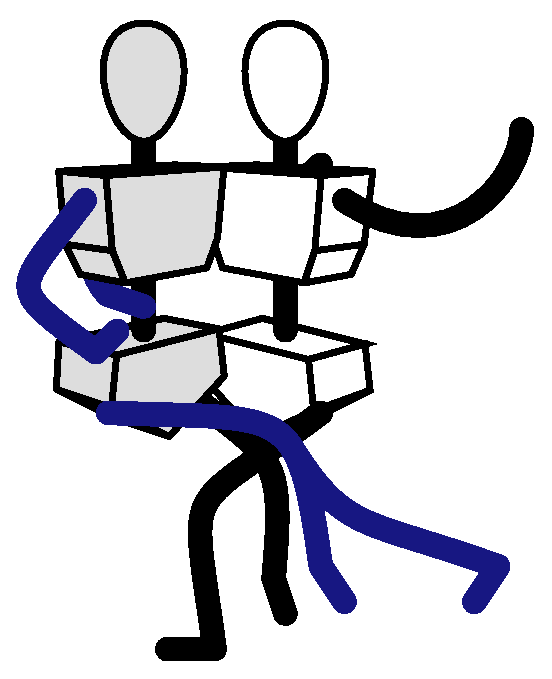
\includegraphics[width=0.23\textwidth]{chapters/cap-historia-passos/cadeirinha.eps}
  \caption{Pose final da  cadeirinha.}
  \label{fig:cadeirinhastickman}
  \vspace{-10pt}
\end{wrapfigure}
No \AnoLivro, o nome cadeirinha representa de forma particular a uma postura onde o \hyperref[def:Seguidor]{\textbf{seguidor}} 
senta-se sobre a perna do \hyperref[def:Condutor]{\textbf{condutor}}  (comumente sobre a perna esquerda);
por outro lado, de forma mais geral  o nome representa a qualquer movimento que tenha como final a 
\hyperref[def:cadeirinha-position]{\textbf{posição de cadeirinha}}.

A saída do chão do seguidor pode-se originar desde vários movimentos ou passos,
como por exemplo do  \hyperref[def:PassoBalao]{\textbf{balão}}; 
porem,
todos conservam a mesma técnica, que ao igual que  no caso do passo  \hyperref[def:PassoElevador]{\textbf{elevador}},
a suspensão no ar do seguidor, é mantida e sustentada pelo braço esquerdo do condutor,
que para este propósito  desce da linha dos ombros.
É importante lembrar que este braço não faz força para levantar ao seguidor, 
e sim simplesmente tenta manter a postura,
o que misturado com o movimento do corpo do condutor (esticar as pernas anteriormente flexionadas, principalmente)
provoca a saída do chão e suspensão do seguidor.
A Figura \ref{fig:cadeirinhastickman} mostra um desenho onde se observa a pose final da cadeirinha.


%%%%%%%%%%%%%%%%%%%%%%%%%%%%%%%%%%%%%%%%%%%%%%%%%%%%%%%%%%%%%%%%%%%%%%%%%%%%%%%
\subsection{Bicicleta}
\index{Passo!Bicicleta}

%%                CICLICO     |SIMETRICO      |CONTRATEMPO   |DESLOCAMENTOS |TIEMPOS
\caracterpasso{\NoCheckedItem}{\NoCheckedItem}{\NoCheckedItem}{\NoCheckedItem}{2}
Movimento sem data de criação conhecida \cite[pp. 143,144]{perna2002samba}.
Porem, podemos ver uma menção a este movimento, junto a outros conhecidos no samba de gafieira, 
em 1979 na revista ``Isto é'' \cite[pp. 89]{revista1979isto}.

No \AnoLivro, o nome bicicleta representa a um movimento da família das escovinhas,
especialmente emparentado com o tipo de escovinhas que chutam para atrás.
Uma vez entrado no movimento da bicicleta é possível pedalar (ou escovar) indefinidamente;
porem isto é pouco comum, na pratica é comum ver só 3 chutes (em 2 tempos) ou 5 chutes (em 3 tempos) ,
pelo que no movimento, mesmo tendo a possibilidade, 
não se executam as pedaladas ou escovadas da contraparte simétrica do primeiro grupo de 3 chutes,
que levariam a completar um ciclo;
pois isto obrigaria a alongar a duração do movimento a mais de 3 tempos,
o que jogaria em contra do espirito deste que é a surpresa.

Existem varias formas para chegar à posição inicial da bicicleta,  
a forma mais simples é a partir do \hyperref[def:abracodedanca]{\textbf{abraço de dança}},
estando o par, frente a frente, 
e com o peso do corpo no lado do pé esquerdo do \hyperref[def:Condutor]{\textbf{condutor}}.
Nesse momento, se o condutor é quem realizará a bicicleta, 
este leva o pé direito atrás,
deixando numa postura estática ao \hyperref[def:Seguidor]{\textbf{seguidor}} 
que servirá de apoio ou referencia;   
o condutor estará ligeiramente inclinado,
procurando ficar numa postura perpendicular entre os planos frontais de ambos dançarinos.
É nesse ponto que o condutor, escova 3 vesses para atrás iniciando com o pé direito,
no tempos 1, 1.5 e 2. No casos que sejam 5 escovadas, se chuta nos tempos,
1, 1.5, 2, 2.5 e 3. No final o condutor termina com o peso do corpo na perna direita,
e pode sair dessa postura, uma forma interessante é fazendo ambos uma tesoura.

%%%%%%%%%%%%%%%%%%%%%%%%%%%%%%%%%%%%%%%%%%%%%%%%%%%%%%%%%%%%%%%%%%%%%%%%%%%%%%%
%%%%%%%%%%%%%%%%%%%%%%%%%%%%%%%%%%%%%%%%%%%%%%%%%%%%%%%%%%%%%%%%%%%%%%%%%%%%%%%
\PRLsep{Passos no samba de gafieira anteriores a 1990}

%%%%%%%%%%%%%%%%%%%%%%%%%%%%%%%%%%%%%%%%%%%%%%%%%%%%%%%%%%%%%%%%%%%%%%%%%%%%%%%
\subsection{ Picadinho (Picadilho)}
\index{Passo!Picadilho}
\index{Passo!Picadinho}
\index{Passo cíclico!Picadinho}
\index{Passo simétrico!Picadinho}
\index{Passo de deslocamento!Picadinho}


Em palavras de Jimmy de Oliveira este movimento já existia antes de 1990 \cite{sambafunkeadoJimmyDeOliveiraPart1}.
Na década de 1920, podemos ver na revista ``A Cigarra'', 
referencias a um tipo de música e de dança denominado picadinho,
geralmente indicado com frases como \cite[pp. 13]{picadinho1}:
\begin{citando}
O chefe da turma é Zezé de Almeida, excellente pianista,
que nos entontece, quando toca os seus \textbf{picadinhos} apimentados;~\\
$[$...$]$~\\
é o Deco. Que rapasinho admiravel.. para dansar \textbf{picadinho}! 
Zezé tocando e Deco dansando, tenho eu divertimento 
para toda a vida e mais seis mezes.
\end{citando}
Em números posteriores da revista, 
podemos achar outras referencias ao picadinho como dança \cite[pp. 52]{picadinho2} \cite[pp. 49]{picadinho3}.


O picadilho ou picadinho, no \AnoLivro~ é um movimento de pouco deslocamento, 
se realiza com um abraço mais folgado, 
para dar espaço ao movimento do \hyperref[def:Seguidor]{\textbf{seguidor}}.
Cada ciclo do movimente dura 4 tempos, sendo o primeiro par de tempos do passo, simétrico ao segundo.

%%                CICLICO     |SIMETRICO   |CONTRATEMPO   |DESLOCAMENTOS |TIEMPOS
\caracterpasso{\CheckedItem}{\CheckedItem}{\NoCheckedItem}{\CheckedItem}{4}
Para uma correta execução do movimento, 
o \hyperref[def:Condutor]{\textbf{condutor}} envia informação de condução mediante o 
\hyperref[def:abracodedanca]{\textbf{abraço de dança}},
de modo que esta informação chegue quase sem degradação ate o quadril do seguidor,
é nesse ponto que a condução provoca o movimento das pernas (uma por vez), de modo que
o seguidor mantêm em todo momento as ``pernas fechadas''\footnote{
Ter as pernas fechadas, neste contexto, não indica literalmente ter as pernas juntas, 
e sim juntar as pernas como se em todo momento ao caminhar tentássemos segurar uma folha de papel na virilha.}.
Assim, na primeira metade do ciclo do passo, no tempo 1, o seguidor,
da inicialmente um passo ao frente ganhando o peso do corpo, 
logo no tempo 1.5 o pé livre que está atrás faz um movimento para fechar mais as pernas, 
ganhando este pé o peso do corpo; finalmente, o novo pé livre se movimenta ligeiramente ao frente no tempo 2, 
para ajeitar a postura e ganhar o peso do corpo, neste caso se descansa um tempo 2 completo.
A segunda metade do ciclo é similar à primeira e inicia no tempo 3, só que agora se começa com o outro pé, 
o pé livre do peso do corpo.


%%%%%%%%%%%%%%%%%%%%%%%%%%%%%%%%%%%%%%%%%%%%%%%%%%%%%%%%%%%%%%%%%%%%%%%%%%%%%%%
%%%%%%%%%%%%%%%%%%%%%%%%%%%%%%%%%%%%%%%%%%%%%%%%%%%%%%%%%%%%%%%%%%%%%%%%%%%%%%%
\PRLsep{Passos de samba de gafieira nas décadas 1980 e 1990}

%%%%%%%%%%%%%%%%%%%%%%%%%%%%%%%%%%%%%%%%%%%%%%%%%%%%%%%%%%%%%%%%%%%%%%%%%%%%%%%
\subsection{Caminhada a contratempo}
\index{Passo!Caminhada a contratempo}
\index{Passo cíclico!Caminhada a contratempo}
\index{Passo a contratempo!Caminhada a contratempo}
\index{Passo de deslocamento!Caminhada a contratempo}
%%                CICLICO     |SIMETRICO   |CONTRATEMPO   |DESLOCAMENTOS |TIEMPOS
\caracterpasso{\CheckedItem}{\NoCheckedItem}{\CheckedItem}{\CheckedItem}{3}
A caminhada a contratempo ou simplesmente caminhada é
uma passo que foi  criado\footnote{Marco Antonio Perna no seu livro 
``Samba de gafieira: A historia da dança de salão brasileira''
só indica o nome caminhada, que é ambíguo pois existem vários 
movimentos que podem ser chamados desse jeito; porém, no
DVD que vem adjunto ao livro e no canal de 
\href{https://www.youtube.com/watch?v=Bke_poU6NBc}{youtube} de Marco Antonio,
pode ser visto que a caminhada corresponde com o passo caminhada a contratempo.} 
entre o final da década de 1980 e inícios de 1990  \cite[pp. 143]{perna2002samba}.
A caminhada a contratempo, no \AnoLivro, 
é um \hyperref[def:PassoCiclico]{\textbf{passo cíclico}} e 
um movimento de deslocamento que dura 3 tempos;
este inicia e finaliza na \hyperref[def:X-position]{\textbf{posição de X}} e usa em todo momento 
um \hyperref[def:abracodedanca]{\textbf{abraço de dança}} na 
\hyperref[def:open-position]{\textbf{posição aberta}}.

Para atingir o tempo 1 o \hyperref[def:Condutor]{\textbf{condutor}} mexe a perna esquerda para adiante, 
e o \hyperref[def:Seguidor]{\textbf{seguidor}}  a direita para atrás,
chegando o par a uma \hyperref[def:frente-frente-position]{\textbf{posição frente a frente}}
com o peso do corpo do lado da perna esquerda do condutor.
Para atingir o tempo 1.5 o condutor cruza a perna direita atrás da esquerda,
e o seguidor a esquerda adiante da direita, levando o peso do corpo com este movimento.
Para atingir o tempo 2 o condutor mexe a perna esquerda, e o seguidor a direita,
descruzando suas pernas, seguindo o fluxo e direção do movimento,
chegando a uma \hyperref[def:frente-frente-position]{\textbf{posição frente a frente}}
com o peso do corpo do lado da perna esquerda do condutor.
Finalmente, para atingir o tempo 3 o condutor mexe a perna direita adiante da esquerda,
e o seguidor a esquerda atrás da direita, 
seguindo o fluxo e direção do movimento para chegar a uma posição de X. 

%%%%%%%%%%%%%%%%%%%%%%%%%%%%%%%%%%%%%%%%%%%%%%%%%%%%%%%%%%%%%%%%%%%%%%%%%%%%%%%
\begin{comment}
\subsection{\textcolor{blue}{Chicote}} 
\index{Passo!Chicote}
Este passo foi  criado entre o final da década de 1980 e inícios de 1990  \cite[pp. 143]{perna2002samba}.
\end{comment}

%%%%%%%%%%%%%%%%%%%%%%%%%%%%%%%%%%%%%%%%%%%%%%%%%%%%%%%%%%%%%%%%%%%%%%%%%%%%%%%
\subsection{\textcolor{blue}{Giro da dama}}
\index{Passo!Giro da dama}
Movimento criado por Jaime Arôxa, entre os anos de 1987 a 1990 \cite{EntrevistaJaimeAroxa1},
sendo este um movimento considerado de nível básico \cite[pp. 144]{perna2002samba}.


%%%%%%%%%%%%%%%%%%%%%%%%%%%%%%%%%%%%%%%%%%%%%%%%%%%%%%%%%%%%%%%%%%%%%%%%%%%%%%%
\subsection{\textcolor{blue}{Tirada de perna}}
\index{Passo!Tirada de perna}
Movimento criado por Jaime Arôxa, entre os anos de 1987 a 1990,
este movimento teve influencias das aulas de tango ditadas por Jaime \cite{EntrevistaJaimeAroxa1},
sendo este um movimento considerado de nível intermediaria \cite[pp. 144]{perna2002samba}.

%%%%%%%%%%%%%%%%%%%%%%%%%%%%%%%%%%%%%%%%%%%%%%%%%%%%%%%%%%%%%%%%%%%%%%%%%%%%%%%
\subsection{\textcolor{blue}{Esse}}
\index{Passo cíclico!Esse} 
\index{Passo!Esse}
Este passo foi  criado entre o final da década de 1980 e inícios de 1990  \cite[pp. 143]{perna2002samba}.

%%%%%%%%%%%%%%%%%%%%%%%%%%%%%%%%%%%%%%%%%%%%%%%%%%%%%%%%%%%%%%%%%%%%%%%%%%%%%%%
\subsection{Facão}
\label{subsec:desc:passo:facao}
\index{Passo!Facão}
\index{Posição!Posição de facão}
\index{Posição de finalização!Posição de facão}

%%                FINALIZA     |TRANSIÇÂO
\caracterpostura{\CheckedItem}{\NoCheckedItem}
Esta posição ou passo foi  criado entre o final da década de 1980 e inícios de 1990  \cite[pp. 143]{perna2002samba}.
Porem na década de 1950 existia um movimento que tinha um final semelhante a esta posição, 
este se chamava ``joelhada'' \cite[pp. 160]{fornaciari1950aprender};
porem, o abraço  não era colado,
e sim mais aberto de modo que o casal terminava tendo contato só nos joelhos.
Assim, a joelhada pode ter sido o precursor ou quem inspirou a criação do facão.

\begin{wrapfigure}{r}{0.25\textwidth}
  \vspace{-10pt}
  \centering
    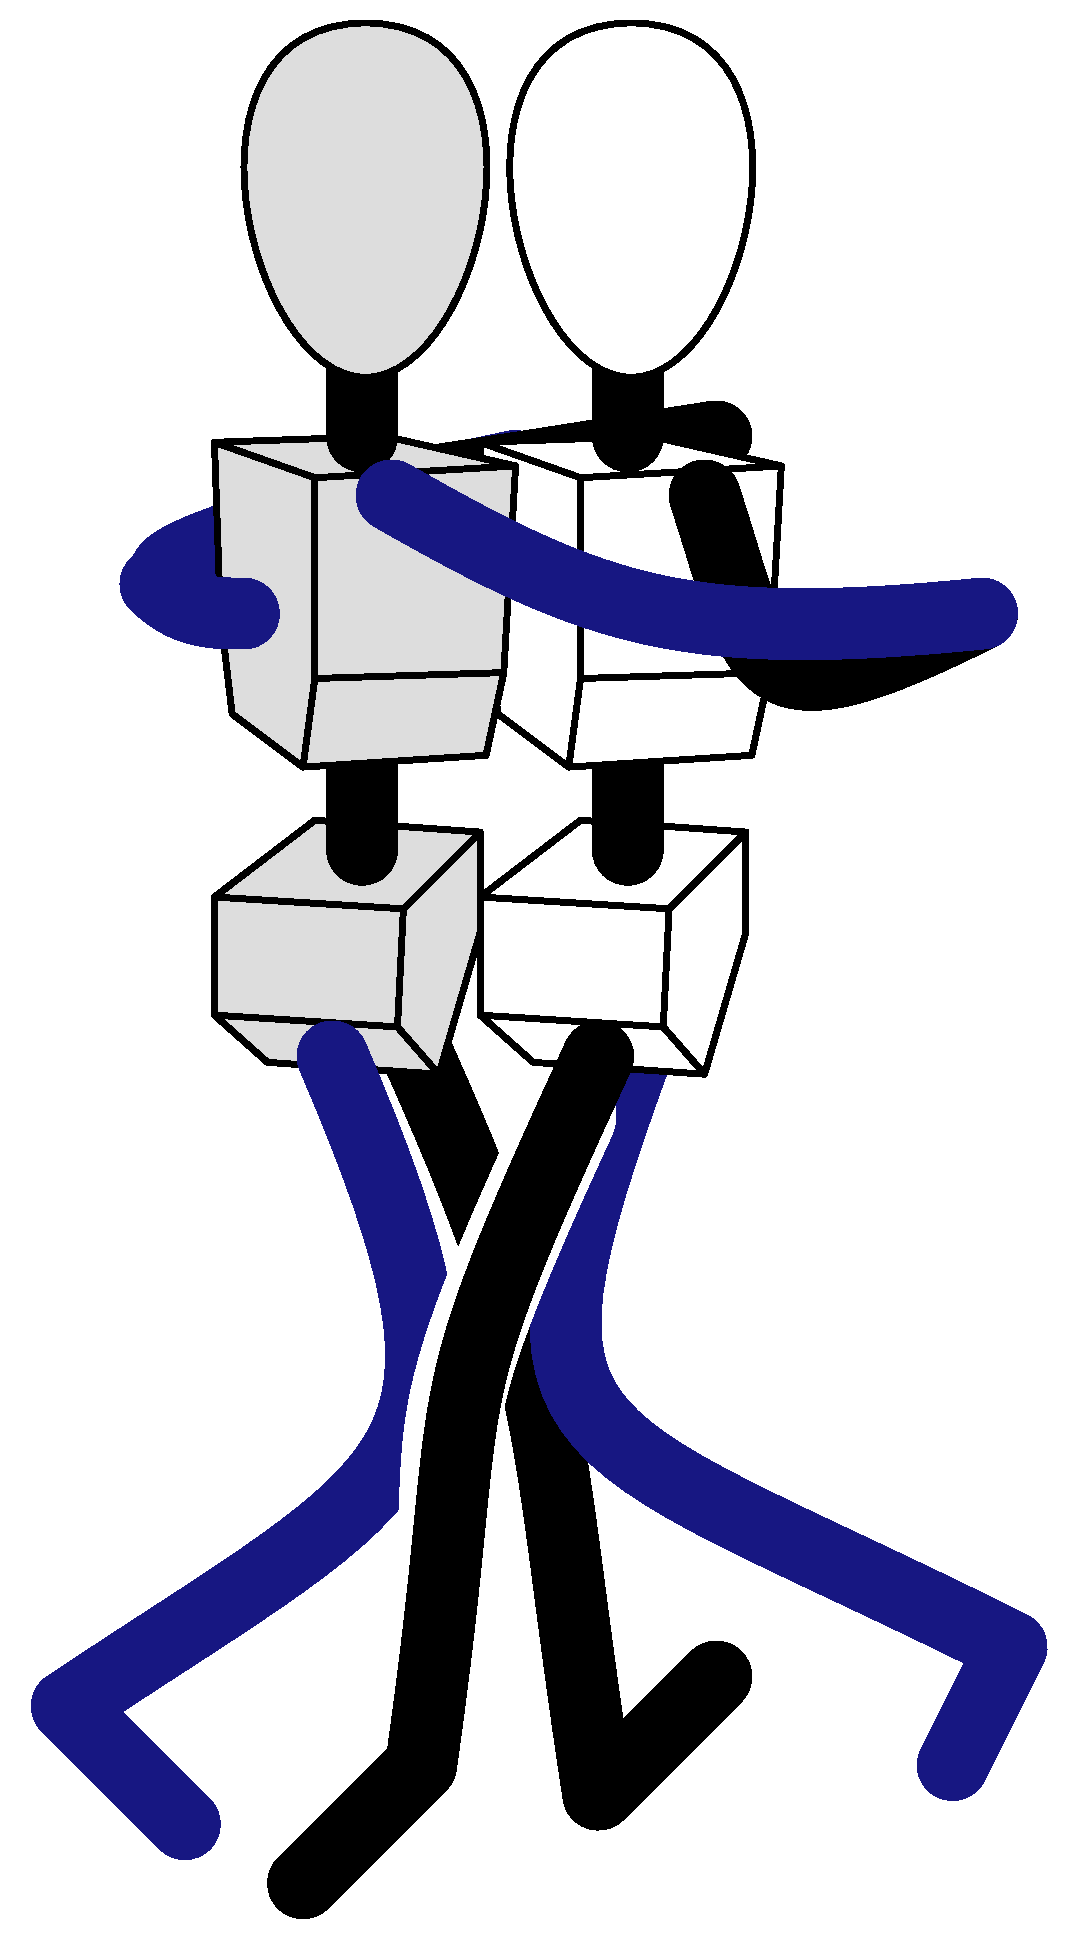
\includegraphics[width=0.23\textwidth]{chapters/cap-historia-passos/facao.eps}
  \caption{Pose final do facão.}
  \label{fig:facaostickman}
  \vspace{-10pt}
\end{wrapfigure}
Voltando ao facão de \AnoLivro, pessoalmente entendo mais este como uma posição que 
como um movimento ou passo. 
Isto é porque existem varias formas pra chegar à \hyperref[def:facao-position]{\textbf{posição de facão}},
de modo que é difícil apontar uma delas para assumir o nome de facão sobre as outras.

A posição do facão, é uma onde o par de dança está num abraçado colado e frente a frente, 
de modo que ambos tem a perna direita um pouco atrás do \hyperref[def:PlanoFrontal]{\textbf{plano frontal}} da linha da cabeça,
e a perna esquerda um pouco adiante no mesmo plano; com esta descrição se deduz 
que ambos tem o peso do corpo dividido em ambos pés; pelo que esta postura,
deve entende-se como uma de descanso, momentâneo porem descanso;
é dizer, se nossa dança fosse um relato escrito, a posição do facão
representaria um ponto, ou em alguns casos um ponto e virgula.
Se o que pretendemos representar é um ponto e virgula, 
é interessante não dividir o peso do corpo 50\% e 50\% em ambos pés,
e sim carregar o peso do corpo um pouco mais em um 
para poder liberar facilmente u outro pé para poder sair elegantemente da posição de facão.  

Sobre as formas de chegar a posição de facão, a continuação será descrita a forma mais simples,
porem não a mais interessante. Iniciamos desde o passo, frente-trás também chamado básico, 
ou básico linear no samba de gafieira. Desde o ponto de vista do \hyperref[def:Condutor]{\textbf{condutor}}, 
com um \hyperref[def:abracodedanca]{\textbf{abraço de dança}} colado,
damos primeiro duas pisadas no lugar, iniciando com a perna esquerda no tempo 1, e logo a perna direita no tempo 1.5,
logo damos um passo atrás com a perna direita no tempo 2; 
finalmente no tempo 3 damos mais um passo atrás com a perna direita, 
e se temos mantido o abraço colado, 
o \hyperref[def:Seguidor]{\textbf{seguidor}} sentirá a necessidade de dar um passo a frente com a perna esquerda,
chegando ambos à posição de facão.  

Este movimento linear para atrás e pouco interessante para chegar ao facão, mas pode ser apimentado,
se usamos um movimento sinuoso para atrás (em vez de um linear), este movimento,
é promovido pelo condutor, e tem forma de ``S'' onde a ligeira curva para a esquerda é realizada no tempo 1 e 1.5,
no tempo  2 chegamos ao ponto neutro o meio, onde a curva esta sobre a linha reta, e para chegar a 3, 
que também está sobre a linha reta e ao final de ambas curvas,
o condutor promove a curva para a sua direita.

%%%%%%%%%%%%%%%%%%%%%%%%%%%%%%%%%%%%%%%%%%%%%%%%%%%%%%%%%%%%%%%%%%%%%%%%%%%%%%%
\subsection{Faquinha}
\index{Passo!Faquinha}
\index{Passo de deslocamento!Faquinha}
\index{Passo cíclico!Faquinha}
%%                CICLICO     |SIMETRICO   |CONTRATEMPO   |DESLOCAMENTOS |TIEMPOS
\caracterpasso{\CheckedItem}{\NoCheckedItem}{\NoCheckedItem}{\CheckedItem}{2}
Este passo foi  criado entre o final da década de 1980 e inícios de 1990  \cite[pp. 143]{perna2002samba}.
É uma variante do  \hyperref[subsec:desc:passo:facao]{\textbf{facão}} (passo), 
com a diferencia que o movimento tem uma posição final (facão) menos acentuada;
sendo mais parecido a um casal num \hyperref[def:abracodedanca]{\textbf{abraço de dança}} colado, 
na \hyperref[def:frente-frente-position]{\textbf{posição frente a frente}}  e com uma perna ligeiramente adiantada a outra;
com diferencia da \hyperref[def:facao-position]{\textbf{posição de facão}}, 
onde as pernas tem uma separação que claramente evidencia uma posição do descanso;
a faquinha, pelo contrario, termina numa posição final de transição, 
pois comumente são realizadas varias faquinhas de forma consecutiva antes de realizar um facão,
 para assim finalizar a sequencia de forma mais acentuada.

O passo faquinha dura dois tempos, e consta de dois movimentos, 
onde a posição final é igual à inicial de modo que o passo pode repetir-se ciclicamente indefinidamente.
O movimento inicia quando o par de dança está numa posição de facão pouco acentuada;
é dizer, quando cada um tem pouca separação entre os pés; 
e o peso do corpo está do lado da perna direita do \hyperref[def:Condutor]{\textbf{condutor}}.
Logo, no primeiro tempo, 
o condutor junta os pés trazendo sua pé esquerdo junto à direito e trocando o peso do corpo a esse pé,
mantendo o abraço para provocar um movimento simétrico no \hyperref[def:Seguidor]{\textbf{seguidor}};
porem a ação do movimento dos pés não é uma causa e sim um efeito,
pois é provocado por uma condução do tórax usando que é transmitida por médio do abraço colado;
para isto o condutor gira o tórax no sentido horário no \hyperref[def:PlanoAxial]{\textbf{plano axial}},
tentando suspender ligeiramente o corpo do seguidor e o seu próprio.
No segundo tempo, o condutor dá um passo atrás com sua perna direita,
 mantendo o abraço colado e provocando que o seguidor de um passo adiante com sua perna esquerda,
chegando novamente a posição inicial.



%%%%%%%%%%%%%%%%%%%%%%%%%%%%%%%%%%%%%%%%%%%%%%%%%%%%%%%%%%%%%%%%%%%%%%%%%%%%%%%
\subsection{\textcolor{blue}{Gancho}} 
\index{Passo!Gancho}
Este passo foi  criado entre o final da década de 1980 e inícios de 1990  \cite[pp. 143]{perna2002samba}.

%%%%%%%%%%%%%%%%%%%%%%%%%%%%%%%%%%%%%%%%%%%%%%%%%%%%%%%%%%%%%%%%%%%%%%%%%%%%%%%
\subsection{\textcolor{blue}{Gancho redondo}} 
\index{Passo!Gancho redondo}
Este passo foi  criado entre o final da década de 1980 e inícios de 1990  \cite[pp. 143]{perna2002samba}.

%%%%%%%%%%%%%%%%%%%%%%%%%%%%%%%%%%%%%%%%%%%%%%%%%%%%%%%%%%%%%%%%%%%%%%%%%%%%%%%
\subsection{\textcolor{blue}{Letra}}
\index{Passo!Letra}
Este passo foi  criado entre o final da década de 1980 e inícios de 1990  \cite[pp. 143]{perna2002samba}.

%%%%%%%%%%%%%%%%%%%%%%%%%%%%%%%%%%%%%%%%%%%%%%%%%%%%%%%%%%%%%%%%%%%%%%%%%%%%%%%
\subsection{\textcolor{blue}{Puladinho redondo}} 
\index{Passo!Puladinho redondo}
Este passo foi  criado entre o final da década de 1980 e inícios de 1990  \cite[pp. 143]{perna2002samba}.

%%%%%%%%%%%%%%%%%%%%%%%%%%%%%%%%%%%%%%%%%%%%%%%%%%%%%%%%%%%%%%%%%%%%%%%%%%%%%%%
\subsection{\textcolor{blue}{Trança}}
\index{Passo cíclico!Trança}
\index{Passo!Trança}
Este movimento é antigo, porem Jaime Arôxa trabalhou sobre ele entre os anos de 1987 a 1990,
pois não existia uma didática para o ensino do movimento, 
e era realizado apenas pelos homens; 
de modo que Jaime agregou a parte do seguidor no par de dança  \cite{EntrevistaJaimeAroxa1} \cite[pp. 143]{perna2002samba}.
%%%%%%%%%%%%%%%%%%%%%%%%%%%%%%%%%%%%%%%%%%%%%%%%%%%%%%%%%%%%%%%%%%%%%%%%%%%%%%%
\subsection{\textcolor{blue}{Tesoura}}
\index{Passo!Tesoura}
Movimento criado por Jaime Arôxa, entre os anos de 1987 a 1990 \cite{EntrevistaJaimeAroxa1} \cite[pp. 143]{perna2002samba}.

%%%%%%%%%%%%%%%%%%%%%%%%%%%%%%%%%%%%%%%%%%%%%%%%%%%%%%%%%%%%%%%%%%%%%%%%%%%%%%%
%%%%%%%%%%%%%%%%%%%%%%%%%%%%%%%%%%%%%%%%%%%%%%%%%%%%%%%%%%%%%%%%%%%%%%%%%%%%%%%
\PRLsep{Passos de samba de gafieira da décadas de 1990}

%%%%%%%%%%%%%%%%%%%%%%%%%%%%%%%%%%%%%%%%%%%%%%%%%%%%%%%%%%%%%%%%%%%%%%%%%%%%%%%
\subsection{\textcolor{blue}{Assalto}} 
\index{Passo!Assalto}
\index{Passo cíclico!Assalto}
Este passo foi criado por Jimmy de Oliveira apos o ano 1990 \cite{sambafunkeadoJimmyDeOliveiraPart1}.

%%%%%%%%%%%%%%%%%%%%%%%%%%%%%%%%%%%%%%%%%%%%%%%%%%%%%%%%%%%%%%%%%%%%%%%%%%%%%%%
\subsection{\textcolor{blue}{Boneca}} 
\index{Passo!Boneca}
Este passo foi criado por Jimmy de Oliveira apos o ano 1990 \cite{sambafunkeadoJimmyDeOliveiraPart1}.

%%%%%%%%%%%%%%%%%%%%%%%%%%%%%%%%%%%%%%%%%%%%%%%%%%%%%%%%%%%%%%%%%%%%%%%%%%%%%%%
\subsection{\textcolor{blue}{Elástico}} 
\index{Passo!Elastico}
Este passo foi criado por Jimmy de Oliveira apos o ano 1990 \cite{sambafunkeadoJimmyDeOliveiraPart1}.

%%%%%%%%%%%%%%%%%%%%%%%%%%%%%%%%%%%%%%%%%%%%%%%%%%%%%%%%%%%%%%%%%%%%%%%%%%%%%%%
\subsection{\textcolor{blue}{Escovinha}}
\index{Passo cíclico!Escovinha}
\index{Passo!Escovinha}
Este passo foi criado por Jimmy de Oliveira apos o ano 1990 \cite{sambafunkeadoJimmyDeOliveiraPart1}.

%%%%%%%%%%%%%%%%%%%%%%%%%%%%%%%%%%%%%%%%%%%%%%%%%%%%%%%%%%%%%%%%%%%%%%%%%%%%%%%
\begin{comment}
\subsection{Homem na lua}
Este passo foi criado por Jimmy de Oliveira apos o ano 1990 \cite{sambafunkeadoJimmyDeOliveiraPart1}.
\end{comment}

%%%%%%%%%%%%%%%%%%%%%%%%%%%%%%%%%%%%%%%%%%%%%%%%%%%%%%%%%%%%%%%%%%%%%%%%%%%%%%%
\subsection{\textcolor{blue}{Pescaria}} 
\index{Passo!Pescaria}
Este passo foi criado por Jimmy de Oliveira apos o ano 1990 \cite{sambafunkeadoJimmyDeOliveiraPart1}.

%%%%%%%%%%%%%%%%%%%%%%%%%%%%%%%%%%%%%%%%%%%%%%%%%%%%%%%%%%%%%%%%%%%%%%%%%%%%%%%
\subsection{\textcolor{blue}{Romário}}
\label{subsec:passo:romario}
\index{Passo cíclico!Romário} 
\index{Passo!Romário}
Este passo foi criado por Jimmy de Oliveira apos o ano 1990 \cite{sambafunkeadoJimmyDeOliveiraPart1}.


%%%%%%%%%%%%%%%%%%%%%%%%%%%%%%%%%%%%%%%%%%%%%%%%%%%%%%%%%%%%%%%%%%%%%%%%%%%%%%%
%%%%%%%%%%%%%%%%%%%%%%%%%%%%%%%%%%%%%%%%%%%%%%%%%%%%%%%%%%%%%%%%%%%%%%%%%%%%%%%
\PRLsep{Passos de samba de gafieira sem data conhecida}



%%%%%%%%%%%%%%%%%%%%%%%%%%%%%%%%%%%%%%%%%%%%%%%%%%%%%%%%%%%%%%%%%%%%%%%%%%%%%%%
\subsection{\textcolor{blue}{Balanço}}
\index{Passo!Balanço}
\index{Passo cíclico!Balanço}
Movimento sem data de criação conhecida, 
seguindo Jaime Arôxa o balanço sempre existiu desde do início do século, 
no maxixe \cite{EntrevistaJaimeAroxa1},
sendo este um movimento considerado de nível básico \cite[pp. 144]{perna2002samba}.


%%%%%%%%%%%%%%%%%%%%%%%%%%%%%%%%%%%%%%%%%%%%%%%%%%%%%%%%%%%%%%%%%%%%%%%%%%%%%%%
\subsection{\textcolor{blue}{Saída lateral}}
\index{Passo!Saída lateral}
Movimento sem data de criação conhecida,
sendo este um movimento considerado de nível básico \cite[pp. 144]{perna2002samba}.

%%%%%%%%%%%%%%%%%%%%%%%%%%%%%%%%%%%%%%%%%%%%%%%%%%%%%%%%%%%%%%%%%%%%%%%%%%%%%%%
\subsection{\textcolor{blue}{Tirada ao lado}}
\index{Passo!Tirada ao lado}
Movimento sem data de criação conhecida,
sendo este um movimento considerado de nível básico \cite[pp. 144]{perna2002samba}.

%%%%%%%%%%%%%%%%%%%%%%%%%%%%%%%%%%%%%%%%%%%%%%%%%%%%%%%%%%%%%%%%%%%%%%%%%%%%%%%
\begin{comment}
\subsection{\textcolor{blue}{Mestre sala}}
\index{Passo!Mestre sala}
Movimento sem data de criação conhecida \cite[pp. 144]{perna2002samba}.
\end{comment}


%%%%%%%%%%%%%%%%%%%%%%%%%%%%%%%%%%%%%%%%%%%%%%%%%%%%%%%%%%%%%%%%%%%%%%%%%%%%%%%
\begin{comment}
\subsection{\textcolor{blue}{Enceradeira}}
\index{Passo!Enceradeira}
Movimento sem data de criação conhecida \cite[pp. 144]{perna2002samba}.
\end{comment}



%%%%%%%%%%%%%%%%%%%%%%%%%%%%%%%%%%%%%%%%%%%%%%%%%%%%%%%%%%%%%%%%%%%%%%%%%%%%%%%
%%%%%%%%%%%%%%%%%%%%%%%%%%%%%%%%%%%%%%%%%%%%%%%%%%%%%%%%%%%%%%%%%%%%%%%%%%%%%%%

\begin{comment}
Passos acrobáticos ou para apresentações \cite[pp. 142-143]{perna2002samba}:
\begin{tasks}
\task \textbf{Cabide}, \index{Passo!Cabide} oriundo do rock.
\task \textbf{Baratinha} \index{Passo!Baratinha}
\task \textbf{Enceradeira}, \index{Passo!Enceradeira} criado em algum momento no final da década de 1980 e inícios da década de 1990.
\end{tasks}
\end{comment}

\newpage
%%%%%%%%%%%%%%%%%%%%%%%%%%%%%%%%%%%%%%%%%%%%%%%%%%%%%%%%%%%%%%%%%%%%%%%%%%%%%%%
%%%%%%%%%%%%%%%%%%%%%%%%%%%%%%%%%%%%%%%%%%%%%%%%%%%%%%%%%%%%%%%%%%%%%%%%%%%%%%%
%%%%%%%%%%%%%%%%%%%%%%%%%%%%%%%%%%%%%%%%%%%%%%%%%%%%%%%%%%%%%%%%%%%%%%%%%%%%%%%
\section{Sobre o $syllabus$ do samba de gafieira}

O $syllabus$  do samba de gafieira, foi criado no ano 2001 em Rio de Janeiro,
este é um listado de passos ordenado em três níveis (básico, intermediário e avançado),
selecionados por votação,
onde são agrupados passos que se consideram essenciais para o ensino e competição;
neste listado não entram passos aéreos \cite[pp. 144]{perna2002samba}.


As personas que participaram da votação para a elaboração do $syllabus$ são \cite[pp. 144]{perna2002samba}:
\begin{inparaitem}[$*$]
\item Bob Cunha e Aurya
\item Bolacha
\item Bruno Barros
\item Carlinhos de Jesus
\item Dani Aguiar
\item Dani Escudero
\item Dani Galper
\item Egídio
\item Flávio Miguel
\item Gérson Reis
\item Kilve
\item Luis Florião/Adriana
\item Marcello Moragas
\item Marco Antonio Perna
\item Marquinhos Copacabana
\item Rogério Mendonça
\item Valdeci
\item Wanir Almeida
\end{inparaitem}.\\



Os passos de \textbf{nível básico} são:
\begin{tasks}(2)
\task Básico (frente-trás)
\task Balanço 
\task Caminhada (ou caminhada a contratempo)
\task Cruzado
\task Esse
\task Gancho
\task Giro da dama
\task Puladinho
\task Saída lateral
\task Tirada ao lado
\end{tasks}~\\


Os passos de \textbf{nível intermediário} são:
\begin{tasks}(2)
\task Assalto
\task Balão apagado
\task Escovinha
\task Facão
\task Gancho redondo
\task Mestre sala
\task Romário
\task Tesoura
\task Tirada de perna
\task Trança
\end{tasks}~\\

Os passos de \textbf{nível avançado} são:
\begin{tasks}(2)
\task Bicicleta
\task Enceradeira
\task Pião
\task Picadinho (ou ou picadilho)
\task Pica-pau
\end{tasks}



\index{Dicionario do samba de gafieira}
\begin{figure}[t]
\begin{elaboracion}[title=Necessidade e alternativas ao Syllabus]

Para o idioma espanhol existe\footnote{\url{https://www.rae.es/la-institucion}} a ``Real Academia Espanhola'' (RAE),
que ``é uma instituição com personalidade jurídica própria, cuja principal missão é garantir 
que as mudanças sofridas pela língua espanhola, 
em sua constante adaptação às necessidades do seus falantes, 
não quebrem a unidade essencial que ela mantém em toda a esfera hispânica".
Nesse sentido a RAE leva registro da língua mediante um \textbf{dicionario},
cuja função é recolher o uso atual da língua, dar um marco comum de comunicação aos falantes de espanhol,
e agregar em suas novas versões, novas palavras ou acepções;
tendo assim um papel de historiador ou cronista e não de regulador estrito do idioma.

Assim, minha opinião pessoal é que para evitar a desconfiança, que alguns profissionais da dança tem,
sobre a instituição de um Syllabus, no sentido  que poderia diminuir a força criativa do samba de gafieira;
podemos em vez instituir, por exemplo, mediante um ``\textbf{Conselho nacional do samba de gafieira}'',
um ``\textbf{Dicionario do samba de gafieira}'', que recolha de forma similar ao Syllabus,
um listado e descrição dos passos mais representativos para a data da liberação de cada edição do dicionario, 
ordenado eles em três níveis (básico, intermediário e avançado) 
com todas as acepções\footnote{Nomes diferentes para um mesmo movimento.}
e outros dados relativos ao samba de gafieira.
De modo que se leve um registro a traves do tempo de como evoluem os movimentos e nomes no samba de gafieira,
e no futuro se alguém o desejar, possa fazer mineração de dados e ver 
por exemplo, como era executado\footnote{Se alguém tem esta curiosidade,
porem para o ano de 1947, a duvida pode ser resolvida no livro
``Como aprender a dançar: novo método de danças modernas'' escrito por Gino Fornaciari \cite[pp. 72]{fornaciari1947aprender}.} 
o movimento que no \AnoLivro~era chamado de ``Pião''.
\end{elaboracion}
\label{fig:ImportanciaSyllabus}
\end{figure}






%----------------------------------------------------------------------------------------
%----------------------------------------------------------------------------------------
%----------------------------------------------------------------------------------------
%	PART
%----------------------------------------------------------------------------------------
\part{Musicalização para a dança}

\chapterimage{chapter_head_teclado.pdf} % Chapter heading image

\chapter{Fundamentos de notação musical}
\label{cap:musicabasica}
Nas seguintes sub seções abordaremos alguns conceitos de notação musical;
porém, não aprofundaremos demasiado em toda a teoria musical, 
devido a que as explicações mostradas aqui, estão
orientadas para um público interessado na dança, que numa primeira 
aproximação à música, precisa conhecer rapidamente conceitos básicos. 
Mas, empoderamos a curiosidade de todos os leitores a aprofundar mais nestos temas, 
para este efeito existem na literatura muitos materiais, livros ou revistas especializadas 
\cite{medteoria}        %% Teoria Da Musica
\cite{cardoso1973curso} %% Curso Completo De Teoria Musical E Solfejo - 1o Vol.
\cite{mascarenhascurso} %% Curso Completo De Teoria Musical E Solfejo - 2o Vol.
\cite{grabner2001teoria}%% Teoría general de la música 
\cite{alves2004teoria}  %% teoria musical lições essenciais
\cite{apel1969harvard}  %% harvard diccionario
\cite{azevedocompor}    %% Como Compor Música Facilmente: métodos ou estudos para teoria, canto e solfejo (NOPDF)
\cite{adolfo2002musica}.%% Musica: Leitura, Conceitos, Exercicios (NOPDF)

%%%%%%%%%%%%%%%%%%%%%%%%%%%%%%%%%%%%%%%%%%%%%%%%%%%%%%%%%%%%%%%%%%%%%%%%%%%%%%%%

%%%%%%%%%%%%%%%%%%%%%%%%%%%%%%%%%%%%%%%%%%%%%%%%%%%%%%%%%%%%%%%%%%%%%%%%%%%%%%%%
\section{Componentes da música}

A música; na sua forma mais básica,  é um conjunto de sons; esta é criada ao combinar na justa medida: 
ingênio, técnica e arte.

Entre as características de um som temos \cite[pp. 12]{medteoria} :
\begin{description}
\item [Altura:] \label{sec:pos:Altura} 
Também chamado \textbf{tom}\footnote{A palavra tom tem vários significados em música, 
outro significado pode ser um intervalo ou distancia em frequência, 
utilizado na escala diatônica, para mais detalhes ir a Seção \ref{sec:notasmusicais}}, representa a frequência de vibração (principal) da onda mecânica que gera o sonido.
Isto é, que terão um altura maior os sonidos com maior frequência de vibração mecânica (mais agudos), 
e uma altura menor sonidos mais graves.
\begin{example}
A campainha pra chamar ao atendente de um hotel tem uma altura maior,
que a campana da igreja, que é tocada ao médio dia, que tem um sonido mais grave.
\end{example} 
\index{Altura}\index{Tom}
\item [Duração:] \label{sec:pos:Duracion}
Representa a longitude temporal, durante o qual um sonido será executado.
\begin{example}
Podemos assoviar durante um tempo, curto, longo, muito longo, etc.
\end{example} 
\index{Duração}
\item [Intensidade:] \label{sec:pos:Intensidade}
Se refere ao volume sonoro ou à potencia do sonido executado, 
de modo que o som pode ter intensidades, por exemplo: fracas, fortes, muito fortes, etc.  
\begin{example}
Si escolhemos dois pedaços de madeira e batimos eles um contra outro, 
podemos gerar sons com diferente intensidade, dependendo da força com que realizemos os batimentos.
\end{example} 
\index{Intensidade}
\item [Timbre:] \label{sec:pos:timbre}
Na definição da altura de um som, referenciamos esta seguindo a sua frequência principal,
porem um som não está composto exclusivamente por vibrações a esta frequência.
Na pratica os sons contem muitas outras frequências de vibração, acontecendo simultaneamente e 
que se manifestam com menor intensidade.
A combinação de todas estas frequências de vibração é o que gera o som que escutamos;
assim, a essa especifica configuração de frequências a chamamos como o timbre ou
a ``\textbf{cor}'' do som.
\begin{example}
Se geramos dois sonidos com a mesma altura; mas, um sonido executado por uma flauta,
e o outro por um violão, ambos sonidos terão diferentes timbres ou cores.
\end{example} 
\index{Timbre}
\end{description}
~\\

Conhecidas estas definições básicas, e procurando estruturas mais complexas na música,
podemos distinguir alguns componentes com que esta é constituída, 
por exemplo temos:

\begin{description}
\item [Ritmo:] \label{sec:pos:Ritmo}
Se refere a distribuição temporal da execução dos sonidos e a proporção na duração destes. 
Asim, o ritmo carateriza a música no âmbito temporal \cite[pp. 11]{medteoria}.
\index{Ritmo}
\begin{example}
Batendo palmas, criamos a sequencia de sonidos: palmas, pausa curta, palmas, palmas, pausa loga e palmas.
\end{example} 
\item [Melodia:] \label{sec:pos:Melodia}
É um conjunto de sons, que podem ter diferentes \hyperref[sec:pos:Altura]{\textbf{alturas}}, 
e que estão dispostos sequencialmente. 
A melodia representa um elemento horizontal\footnote{\label{eixohor}Eixo com múltiplas distribuições de tempo dos sons na música} na musica, 
e esta é indivisível do ritmo \cite[pp. 517]{apel1969harvard} \cite[pp. 11]{medteoria}.
\begin{example}
Se assoviamos ``parabéns pra você'', estamos executando uma melodia 
(executando diferentes sons numa distribuição temporal especifica).
\end{example} 
\index{Melodia} 
\item [Harmonia:] \label{sec:pos:Harmonia}
Conjunto de sons dispostos simultaneamente em \hyperref[sec:pos:Altura]{\textbf{alturas}} diferentes.
A harmonia representa um elemento vertical\footnote{\label{eixover}Eixo com múltiplas distribuições de frequência dos sons na música} na música \cite[pp. 371]{apel1969harvard} \cite[pp. 8]{cardoso1973curso} \cite[pp. 11]{medteoria}. 
\begin{example}
Se num piano pressionamos simultaneamente as teclas: Do, Mi e Sol. Estamos executando uma harmonia.
\end{example} 
\index{Harmonia} 
\item [Contraponto:] \label{sec:pos:Contraponto}
O termo deriva de ``punctus contra punctum'' que significa ``nota contra nota'', 
e por extensão ``melodia contra melodia''. 
Assim, falar de contraponto é equivalente a dizer, dois ou mais melodias executadas simultaneamente  
(concepção horizontal\footref{eixohor} e vertical\footref{eixover} da música)  \cite[pp. 208]{apel1969harvard} \cite[pp. 11]{medteoria}.
\begin{example}
Uma orquestra com vários músicos tocando cada um uma melodia.
\end{example} 
\index{Contraponto}
\end{description}


 
%%%%%%%%%%%%%%%%%%%%%%%%%%%%%%%%%%%%%%%%%%%%%%%%%%%%%%%%%%%%%%%%%%%%%%%%%%%%%%%%
\section{Figuras musicais, pausas e durações}
\index{Música!Figuras musicais}
\index{Música!Figuras rítmicas}
\label{sec:figurasmusicais}
As figuras musicais também chamada figuras rítmicas \cite[pp. 16]{alves2004teoria}, 
são um conjunto de sinais (desenhos), criadas pra indicar a relação 
entre as \hyperref[sec:pos:Duracion]{\textbf{durações}} dos sons \cite[pp. 20]{medteoria}.
Assim, podemos ver na coluna dois da Tabela \ref{tab:abc-noteslengthbasic}
 um conjunto de 6 destas figuras musicais; 
a primeira coluna representa a longitude temporal (\hyperref[sec:pos:Duracion]{\textbf{duração}}) de cada uma destas figuras;
porém, todos estas durações são relativas ao valor temporal $S$, em segundos, de uma figura \Ganz.
A terceira coluna da tabela contem os nomes de cada uma destas figuras musicais. 
\begin{table}[h]
\centering
\begin{tabular}{|c||c|c||c|c|}
\hline
Duração & Figura & Nome de figura & Pausa & Nome de pausa\\ \hline
\hline
$S$    & \Ganz   & Semibreve    & \GaPa  & Pausa de Semibreve \\ \hline
$S/2$  & \Halb   & Mínima       & \HaPa  & Pausa de Mínima \\ \hline
$S/4$  & \Vier   & Semínima     & \ViPa  & Pausa de Semínima \\ \hline
$S/8$  & \Acht   & Colcheia     & \AcPa  & Pausa de Colcheia \\ \hline
$S/16$ & \Sech   & Semicolcheia & \SePa  & Pausa de Semicolcheia \\ \hline
$S/32$ & \Zwdr   & Fusa         & \ZwPa  & Pausa de fusa  \\ \hline  
\end{tabular}
\caption{Duração e símbolos de algumas figuras musicais}
\label{tab:abc-noteslengthbasic}
\end{table}


\begin{example}
Se decidimos criar uma sequencia rítmica assoviando um único tom, porém
distribuindo os tempos de duração como: Longo, curto, curto; 
repetindo esta sequencia quatro vesses. 
Poderíamos escrever esta sequencia usando figuras musicais numa representação como a mostrada na Figura \ref{fig:abc-figurasexample1}.
É importante ressaltar que assumimos que  um sonido longo dura no tempo exatamente o dobro que um curto, 
e que decidimos\footnote{É escolhida uma semínima porém pode ter sido escolhida 
qualquer outra figura, dado que o valor $S$ não está definido.}
representar um sonido de longa duração como uma semínima.

Para entender melhor a representação com figuras musicais, 
podemos ir a uma representação alternativa com um gráfico da potencia sonora na execução dos sons,
como é representado na Figura \ref{fig:forma-figurasexample1b}.
É fácil perceber como a potencia do som se mantêm, ate justo antes de iniciar 
o seguinte som, de modo que não existem silêncios na sequencia rítmica.
\end{example} 




\begin{figure}[h]
    \centering
    \begin{subfigure}[b]{0.9\textwidth}
 \begin{abc}[name=abc-figurasexample1]
% abcm2ps figurasexample1.abc  -O figurasexample1.ps
% ps2epsi figurasexample1.ps figurasexample1.eps
%
X: 1 % start of header
K: none stafflines=0 %K: C %% Escala de C mayor %
M:  none % M: 2/4
%T: Contratempo num compasso binário
V:1 clef=none stem=up %name="Ritmo 1"   sname="Ritmo 1"
%
[V:1] | B2 B1 B1 B2 B1 B1 B2 B1 B1 B2  B1 B1   |
%       
\end{abc}
	\caption{Sequencia rítmica usando semínimas e colcheias.}
	\label{fig:abc-figurasexample1}
    \end{subfigure}
    ~%add desired spacing between images, e. g. ~, \quad, \qquad, \hfill etc. 
      %(or a blank line to force the subfigure onto a new line)
    \begin{subfigure}[b]{0.9\textwidth}
        \includegraphics[width=\textwidth]{chapters/cap-musica-basica/forma-figurasexample1.eps}
        \caption{Sequencia rítmica usando um gráfico indicando a potencia do sonido.}
        \label{fig:forma-figurasexample1b}
    \end{subfigure}
    \caption{Sequencia rítmica.}\label{fig:total-figurasexample1}
\end{figure}


Por outro lado, assim como a duração do tempo de execução de cada som precisa uma grafia,
os silêncios ou pausas, também precisam ser indicados. 
De modo que, para cada figura musical existe uma grafia que indica um silencio da mesma duração temporal,
como pode ser visto na quarta coluna da Tabela \ref{tab:abc-noteslengthbasic}.
O nome de cada uma destas pausas está descrito na quinta coluna da mesma tabela.

\begin{example}
Similarmente ao exemplo anterior, se decidimos criar uma sequencia rítmica assoviando um único tom, porém
intercalando sons e silêncios, criaremos um padrão rítmico como na Figura \ref{fig:total-figurasexample2}.

Podemos entender melhor a representação com figuras musicais, 
usando a representação com um gráfico da potencia sonora na execução dos sons,
como é representado na Figura \ref{fig:forma-figurasexample2}.
Nela percebemos como a potencia do som se mantêm durante a longitude de tempo estipulada pela figura musical, 
ate justo antes de iniciar o silencio, indicado por uma linha reta horizontal.
\end{example} 

\begin{figure}[h]
    \centering
    \begin{subfigure}[b]{0.9\textwidth}
 \begin{abc}[name=abc-figurasexample2]
% abcm2ps figurasexample2.abc  -O figurasexample2.ps
% ps2epsi figurasexample2.ps figurasexample2.eps
%
X: 1 % start of header
K: none stafflines=0 %K: C %% Escala de C mayor %
M:  none % M: 2/4
%T: Contratempo num compasso binário
V:1 clef=none stem=up %name="Ritmo 1"   sname="Ritmo 1"
%
[V:1] | z1 B1 z1 B1 z2 B1 z1 B1 z1 B1 z2 B1  z1 B1   |
%       
\end{abc}
	\caption{Sequencia rítmica usando  colcheias e silencios.}
	\label{fig:abc-figurasexample2}
    \end{subfigure}
    ~%add desired spacing between images, e. g. ~, \quad, \qquad, \hfill etc. 
      %(or a blank line to force the subfigure onto a new line)
    \begin{subfigure}[b]{0.9\textwidth}
        \includegraphics[width=\textwidth]{chapters/cap-musica-basica/forma-figurasexample2.eps}
        \caption{Sequencia rítmica usando um gráfico indicando a potencia do sonido.}
        \label{fig:forma-figurasexample2}
    \end{subfigure}
    \caption{Sequencia rítmica.}\label{fig:total-figurasexample2}
\end{figure}


Ate agora todos os exemplos foram sequencias rítmicas, 
pois não exploramos a possibilidade de variar a altura dos sons;
para poder explorar esta possibilidade devemos ter claro o conceito de pauta,
para que cada figura musical, 
além de nos proporcionar uma informação da \hyperref[sec:pos:Duracion]{\textbf{duração}}  dos sons, 
também nos de informação da \hyperref[sec:pos:Altura]{\textbf{altura}}  destes. 
Tendo estes dois fatores, altura e duração, podemos criar \hyperref[sec:pos:Melodia]{\textbf{melodias}}.

\begin{tcbattention}
O mistério de como distinguir a pausa de mínima (\HaPa) e a pausa de semibreve (\GaPa),
será esclarecido quando desenhemos estes na \hyperref[sec:pauta]{\textbf{pauta}}, ver Seção \ref{sec:tipospauta}.
\end{tcbattention}

\subsection{Ponto de aumento}
\index{Música!Ponto de aumento}
\label{subsec:pontoaumento}
O ponto de aumento é um simbolo que é colocado ao lado direito de uma figura musical ou pausa, 
e este indica um aumento do 50\% na duração \cite[pp. 25]{cardoso1973curso}.
A Tabela \ref{tab:notaspontoadas} mostra esta relação entre as durações.

\begin{table}[h]
\centering
\begin{tabular}{|c||c||c|}
\hline
Duração & Figura & Pausa \\ \hline
\hline
$\frac{3}{2}S$    & \Ganz. =  \Ganz + \Halb   & \GaPa. = \GaPa + \HaPa\\ \hline
$\frac{3}{4}S$    & \Halb. =  \Halb + \Vier   & \HaPa. = \HaPa + \ViPa  \\ \hline
$\frac{3}{8}S$    & \Vier. =  \Vier + \Acht   & \ViPa. = \ViPa + \AcPa  \\ \hline
$\frac{3}{16}S$   & \Acht. =  \Acht + \Sech   & \AcPa. = \AcPa + \SePa  \\ \hline
$\frac{3}{32}S$   & \Sech. =  \Sech + \Zwdr   & \SePa. = \SePa + \ZwPa  \\ \hline
\end{tabular}
\caption{Duração e símbolos de algumas figuras musicais com ponto de aumento}
\label{tab:notaspontoadas}
\end{table}

Da mesma forma que usamos um ponto de aumento, podem ser usados dois ou três pontos de aumento.
\begin{example}
Se usamos dois pontos de aumento a duração de uma nota cresce um 75\%, assim: \Halb.. = \Halb + \Vier + \Acht
\end{example}
\begin{example}
Se usamos tres pontos de aumento a duração de uma nota cresce um 87.5\%, assim: \Vier... = \Vier + \Acht + \Sech + \Zwdr
\end{example}



     
%%%%%%%%%%%%%%%%%%%%%%%%%%%%%%%%%%%%%%%%%%%%%%%%%%%%%%%%%%%%%%%%%%%%%%%%%%%%%%%%
\section{Notas musicais, tons e escalas}\index{Música!Notas musicais}
\label{sec:notasmusicais}

O sons musicais que representam as notas são sete, 
e foram designadas pelos gregos com as sete primeiras letras do alfabeto,
estes são: \{A, B, C, D, E, F, G\} \cite[pp. 11]{grabner2001teoria} \cite[pp. 9]{cardoso1973curso}.
O ocidente adotou esta forma porem no século XI, 
Guido d'Arezzo rebatizou as notas, 
atribuindo a cada nota a primeira sílaba dos versos
de um hino a São Jõao muito conhecido na época:
\begin{citando}%%
\textbf{Ut} queant laxls,\\
\textbf{re}sonare fibris,\\
\textbf{Mi}ra gestorum,\\
\textbf{fa}muli tuorum,\\
\textbf{Sol}ve polluti,\\
\textbf{La}bii reatum,\\
\textbf{S}ánete lohannes.
\end{citando}
 Assim, apos a troca de ``ut'' por ``do'' nascem as notas musicais: 
\{lá, si, dó, ré, mi, fá, sol\} \cite[pp. 21]{arbones2012armonia} \cite[pp. 7]{cardoso1973curso}. 
A Tabela \ref{tab:notasmusic} mostra a relação entre estas duas notações.

\begin{table}[h]
\centering
\begin{tabular}{|c|c|c|c|c|c|c|}
\hline
A  & B  & C  & D  & E  & F  & G\\ \hline
lá & si & dó & ré & mi & fá & sol \\ \hline
\end{tabular}
\caption{Notas musicais}
\label{tab:notasmusic}
\end{table}

Estas sete notas representam sons com \hyperref[sec:pos:Altura]{\textbf{alturas}} diferentes.
Porem, existem varias formas de atribuir uma \hyperref[sec:pos:Altura]{\textbf{altura}} 
especifica a cada uma destas notas, 
sendo a mais difundida atualmente a afinação (atribuição de alturas) com \hyperref[subsec:tempigual]{\textbf{temperamento igual}}\footnote{O temperamento igual é tratado na Seção \ref{subsec:tempigual}.}.


%%%%%%%%%%%%%%%%%%%%%%%%%%%%%%%%%%%%%%%%%%%%%%%%%%%%%%%%%%%%%%%%%%%%%%%%%%%%%%%%
\subsection{Escalas musicais}

\label{sec:pos:Escala}
\index{Música!Escalas musicais}
As escalas musicais são uma forma de organizar as notas musicais, 
numa ordem que permitam ser lidas de forma crescente em relação a altura dos sons.
Existe uma variedade de escalas musicais usadas em distintas épocas ou países, 
porem a escala básica da música europeia é a escala diatônica. \cite[pp. 753]{apel1969harvard}
\begin{example}As escalas mais conhecidas são:
\begin{inparaitem}
\item Escala diatônica
\item Escala cromática
%\item Escala diatônica no modo jônico
%\item Escala diatônica no modo dórico
%\item Escala diatônica no modo frígio
%\item Escala diatônica no modo lídio
%\item Escala diatônica no modo mixolídio
%\item Escala diatônica no modo eólico
%\item Escala diatônica no modo lócrio
\item Escala pentatônica
\item Escala de blues
\item etc.
\end{inparaitem}
\end{example}

\begin{description}

\item [Escala diatônica:] \label{sec:pos:Diatonica}
\index{Música!Escala diatônica}
Também conhecida como \textbf{escala de C-major},
é uma sucessão de 8 sons,  escritos em sentido ascendente em relação a altura das notas, 
sendo os 7 primeiros sons as notas mostradas na Tabela \ref{tab:notasmusic}, iniciando em dó,
e a oitava nota a repetição da primeira nota, 
porem mais aguda, é dizer com uma frequência igual ao dobro.
Existem 7 distancias entre as 8 notas, medidas em progressão geométrica\footnote{A 
distancia, em progressão geométrica, entre dois números $X$ e $Y$, é obtida calculando o fator $\frac{Y}{X}$. }, 
sendo que estas distancias tem só dois longitudes diferentes, chamadas tons e semitons;
de modo que a separação entre as notas nesta escala é distribuída da seguinte forma: 
tom,tom,semitom,tom,tom,tom,semitom \cite[pp. 30]{cardoso1973curso}\cite[pp. 753]{apel1969harvard}.
\begin{example}
\begin{equation*}
d\acute{o}\overset{tom}{\rightarrow}
r\acute{e}\overset{tom}{\rightarrow}
mi\overset{semitom}{\rightarrow}
f\acute{a}\overset{tom}{\rightarrow}
sol\overset{tom}{\rightarrow}
l\acute{a}\overset{tom}{\rightarrow}
si\overset{semitom}{\rightarrow}
d\acute{o}
\end{equation*}
\end{example}
Para mais detalhes numéricos da escala diatônica ir a Página \pageref{ref:paginadiatonicanumerica}.


\item [Escala cromática:] \label{sec:pos:Cromatica}
\index{Música!Escala cromática}
Também chamada escala dodecafônica ou duodécuple, 
esta escala está constituída por uma sucessão de 12 sons, separados uma distancia de 1 semitom.
Os outros tipos de escalas na música moderna podem ser considerados como subconjuntos desta escala \cite[pp. 753]{apel1969harvard}
\begin{example} 
Se representamos um semitom por ``$\alpha$'', 
e definimos o simbolo $\#$ como indicador de uma nota, um semitom acima, 
então a escala cromática é definida como:\\
$d\acute{o}\overset{\alpha}{\rightarrow}$
$\#d\acute{o}\overset{\alpha}{\rightarrow}$
$r\acute{e}\overset{\alpha}{\rightarrow}$
$\#r\acute{e}\overset{\alpha}{\rightarrow}$
$mi\overset{\alpha}{\rightarrow}$
$f\acute{a}\overset{\alpha}{\rightarrow}$
$\#f\acute{a}\overset{\alpha}{\rightarrow}$
$sol\overset{\alpha}{\rightarrow}$
$\#sol\overset{\alpha}{\rightarrow}$
$l\acute{a}\overset{\alpha}{\rightarrow}$
$\#l\acute{a}\overset{\alpha}{\rightarrow}$
$si$
\end{example}

\end{description}~\\


%%%%%%%%%%%%%%%%%%%%%%%%%%%%%%%%%%%%%%%%%%%%%%%%%%%%%%%%%%%%%%%%%%%%%%%%%%%%%%%%
\subsection{Tom e Semitom}
\label{subsec:tomesemitom}
\index{Música!Tom}
\index{Música!Semitom}

Os tons e semitons são termos usados para designar aos intervalos entre as alturas das notas utilizados na 
\hyperref[sec:pos:Diatonica]{\textbf{escala diatônica}}.
Deve-se ter em conta que quando usamos o nome tom,
podemos nos referir a \hyperref[sec:pos:Altura]{\textbf{altura}} 
de uma nota ou ao intervalo entre algumas notas da escala diatônica;
a continuação usaremos esta última acepção.

\begin{description}

\item [Semitom:] \label{sec:pos:Semitom}
\index{Música!Semitom}
É a menor distancia entre duas notas na música tradicional ocidental.
Na \hyperref[sec:pos:Diatonica]{\textbf{escala diatônica}} 
podem se achar distancias de semitons entre mi e fá, e entre si e dó.
O valor exato de um semitom varia ligeiramente de acordo com o sistema de afinação \cite[pp. 30]{cardoso1973curso}\cite[pp. 762]{apel1969harvard}, ver afinação com temperamento igual na Seção \ref{subsec:tempigual}. 
Em algumas bibliografias se define ao semitom como a ``metade'' de um tom, 
porem esta só é uma forma metafórica de falar, 
pois um semitom não representa a metade do valor numérico de um tom;
em verdade os tons e semitons são calculados considerando que as notas cumprem uma progressão geométrica
(irregular na escala diatônica e regular na escala cromática);
assim, o correto seria falar que: um semitom está na metade do caminho, em progressão geométrica, de um tom\footnote{Na 
afinação com temperamento igual um $Semitom=\sqrt{tom}$}.
\begin{example}
Se numa escala diatônica definimos $f_{mi}$ e $f_{fa}$ como as frequências das notas mi e fá respetivamente.
então o valor de um semitom seria equivalente a,
\begin{equation*}
Semitom=\frac{f_{fa}}{f_{mi}}
\end{equation*}
\end{example}

\item [Tom:] \label{sec:pos:TomDist}
\index{Música!Tom}
É uma distancia, em progressão geométrica, equivalente a duas distancias de semitons colocadas consecutivamente entre duas notas.
Na \hyperref[sec:pos:Diatonica]{\textbf{escala diatônica}} podemos achar distancias de um tom entre todas as notas exceto entre mi e fá, e entre si e dó \cite[pp. 30]{cardoso1973curso}\cite[pp. 762]{apel1969harvard}.
O valor exato de um tom varia ligeiramente de acordo com o sistema de afinação, ver afinação com temperamento igual na Seção \ref{subsec:tempigual}. 
\begin{example}
Se numa escala diatônica definimos $f_{fa}$ e $f_{sol}$ como as frequências das notas fá e sol respetivamente.
então o valor de um tom seria equivalente a,
\begin{equation*}
Tom=\frac{f_{sol}}{f_{fa}}
\end{equation*}
\end{example}

\item [Oitava:] \label{sec:pos:Oitava}
\index{Música!Oitava}
Representa o oitavo tom de uma \hyperref[sec:pos:Diatonica]{\textbf{escala diatônica}}. 
Correspondente  ao tom com o dobro da frequência do tom escolhido como referencia \cite[pp. 589]{apel1969harvard}
\begin{example}~
\begin{itemize}
\item Dado uma nota lá a $440$ hertz, teremos um lá numa oitava superior a uma frequência de $880$ hertz  
\item Dado uma nota lá a $440$ hertz, teremos um lá numa oitava inferior a uma frequência de $220$ hertz  
\end{itemize}
\end{example}

\end{description}~\\

%%%%%%%%%%%%%%%%%%%%%%%%%%%%%%%%%%%%%%%%%%%%%%%%%%%%%%%%%%%%%%%%%%%%%%%%%%%%%%%%
\subsection{Acidentes ou alterações}
\label{subsec:acidentes}
\index{Música!Acidentes}


Os acidentes ou alterações são símbolos que modificam a altura de uma nota; 
os mais utilizado são \cite[pp. ]{alves2004teoria}:\\

\begin{description}

\item [Sustenido ($\#$):] \label{sec:pos:Sustenido}
\index{Música!Sustenido}
É um simbolo u operador que acompanha a uma nota, 
e indica um som com uma altura um semitom acima da nota indicada.
Uma vez usado o símbolo, o âmbito  do simbolo continua ativo, 
para notas do mesmo tom, sem a necessidade de grafar novamente com o símbolo $\#$;
para desabilitar este âmbito, se usa o simbolo $\natural$. 
\begin{example} $\#$dó : é equivalente a dizer, um som um semitom acima de dó.
\end{example}


\item [Bemol ($\flat$):] \label{sec:pos:Bemol}
\index{Música!Bemol}
É um simbolo u operador que acompanha a uma nota, 
e indica um som com uma altura um semitom abaixo da nota indicada. 
Uma vez usado o símbolo, o âmbito  do simbolo continua ativo, 
para notas do mesmo tom, sem a necessidade de grafar novamente com o símbolo $\flat$;
para desabilitar este âmbito, se usa o simbolo $\natural$. 
\begin{example} $\flat$ré : é equivalente a dizer, um som um semitom abaixo de ré.
\end{example}

\item [Bequadro ($\natural$):] \label{sec:pos:Bequadro}
\index{Música!Bequadro}
Este símbolo anula o efeito dos símbolos anteriormente mencionados.

\end{description}~\\

%%%%%%%%%%%%%%%%%%%%%%%%%%%%%%%%%%%%%%%%%%%%%%%%%%%%%%%%%%%%%%%%%%%%%%%%%%%%%%%%
\subsection{Temperamento igual}
\label{subsec:tempigual}
\index{Música!Temperamento igual}
No  temperamento igual se divide uma oitava em doze semitons da mesma distancia.
de modo que qualquer par de notas separadas uma 
\hyperref[sec:pos:Oitava]{\textbf{oitava}} tenham uma distancia igual a $2$ \cite[pp. 835]{apel1969harvard}.
Assim, se temos um par de notas lá, a primeira a uma frequência $f_0$, 
e a outra uma oitava acima com uma frequência $2f_0$;
e sabendo que existem $12$ passos (semitons) em progressão  geométrica para completar uma oitava 
(como mostra a Tabela \ref{tab:temperamento1} na linha 4),
então a distancia $\alpha$ de cada semitom pode ser calculada como:
\begin{equation}
f_0\alpha^{12}\equiv 2 f_0
\end{equation}
\begin{sidewaystable}
\centering
\begin{tabular}{|c|c|c|c|c|c|c|c|c|c|c|c||c|}
\hline
 lá  & ~ & si  & dó  & ~ & ré  & ~ & mi  & fá  & ~ & sol   & ~ & lá\\ \hline
 ~  & $\#$lá  & ~  & ~  & $\#$dó  & ~  & $\#$ré  & ~  & ~  & $\#$fá  & ~   & $\#$sol   & ~\\ \hline
 ~  & $\flat$si  & ~  & ~  &  $\flat$ré  & ~  &  $\flat$mi  & ~  & ~  &  $\flat$sol  & ~   &  $\flat$lá   & ~\\ \hline
$f_0$ & $f_0\alpha$ & $f_0\alpha^2$ & $f_0\alpha^3$ & $f_0\alpha^4$ & $f_0\alpha^5$ & $f_0\alpha^6$ & $f_0\alpha^7$ & $f_0\alpha^8$ & $f_0\alpha^9$ & $f_0\alpha^{10}$ & $f_0\alpha^{11}$ & $f_0\alpha^{12}$ \\ \hline
\end{tabular}
\caption{Temperamento igual em todas as notas da escala cromática.}
\label{tab:temperamento1}
\end{sidewaystable}
de modo que um \hyperref[sec:pos:Semitom]{\textbf{semitom}} ($\alpha$) é igual a,
\begin{equation}
\alpha \equiv \sqrt[12]{2} \approx  1.05946309435930,
\end{equation}
e um \hyperref[sec:pos:TomDist]{\textbf{tom}} ($\alpha^2$) é igual a,
\begin{equation}
\alpha^2 \equiv \sqrt[6]{2} \approx  1.12246204830937,
\end{equation}

Assim, para qualquer nota selecionada na escala, 
se cumpre que a frequência se duplica apos 12 semitons.
No caso da Figura \ref{fig:circulonotas} isto é valido quando avançamos no sentido das agulhas do relógio.
Por outro lado, a frequência se dividirá por dois a cada 12 semitons,
em sentido contrario as agulhas do relógio.
    \begin{figure}[h]
        \centering
        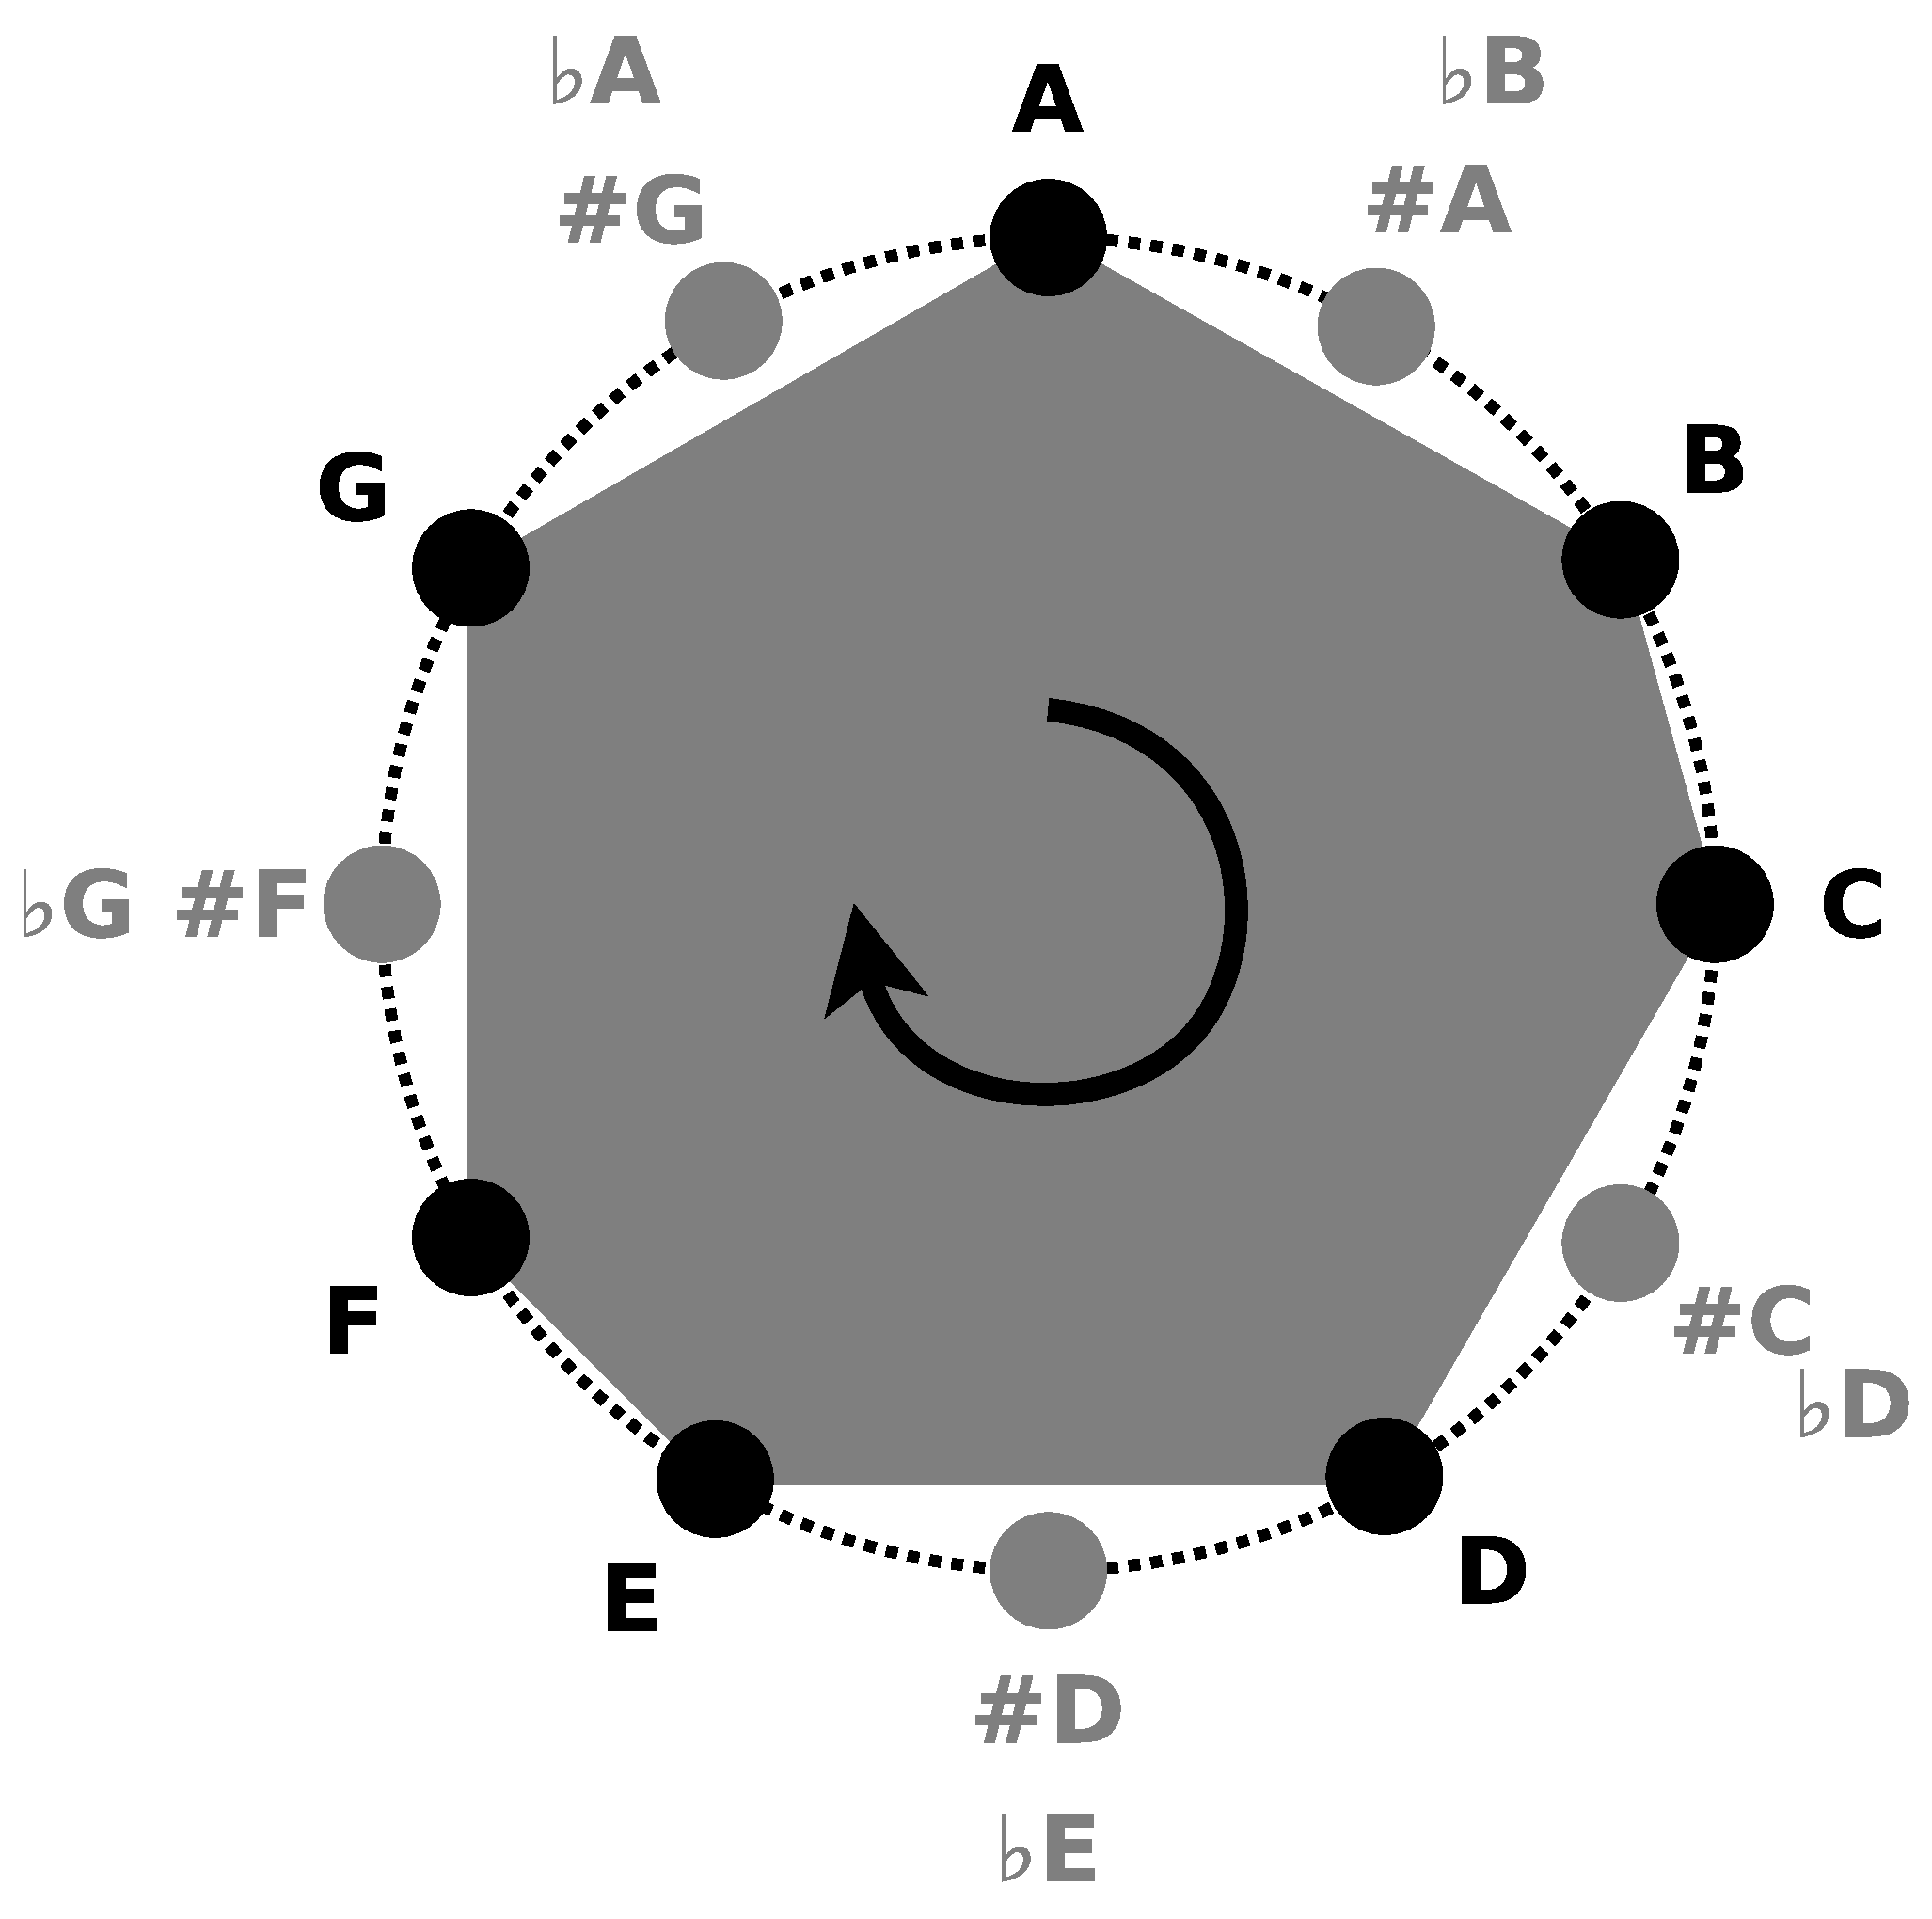
\includegraphics[width=0.65\textwidth]{chapters/cap-musica-basica/circulonotas.eps}
        \caption{Representação cíclica das distancias das notas musicais.}
        \label{fig:circulonotas}
    \end{figure}

Adicionalmente, na Figura \ref{fig:circulonotas}, 
está representada a escala diatônica com uma figura geométrica de 6 lados, 
colorido em cinza; e a escala cromática está representada com um circulo de linha pontuada.


     
%%%%%%%%%%%%%%%%%%%%%%%%%%%%%%%%%%%%%%%%%%%%%%%%%%%%%%%%%%%%%%%%%%%%%%%%%%%%%%%%
\section{\textcolor{blue}{Tipos de pauta}}
\label{sec:tipospauta}

%%%%%%%%%%%%%%%%%%%%%%%%%%%%%%%%%%%%%%%%%%%%%%%%%%%%%%%%%%%%%%%%%%%%%%%%%%%%%%%%
%%%%%%%%%%%%%%%%%%%%%%%%%%%%%%%%%%%%%%%%%%%%%%%%%%%%%%%%%%%%%%%%%%%%%%%%%%%%%%%%
\subsection{Pauta ou Pentagrama}\index{Pauta}
\label{sec:pauta}
A pauta está representada por 5 linhas paralelas e horizontais, 
as figuras musicais podem ocupar as linhas ou um lugar médio, entre elas.
Adicionalmente, lugares fora da pauta podem ser usados; 
para este proposito, linhas adicionais e parcialmente desenhadas, serão colocadas \cite[pp. 10]{cardoso1973curso}
como é mostrado na Figura \ref{fig:abc-pauta5}.
\begin{figure}[H]
\centering
\begin{abc}[name=abc-pauta5]
% abcm2ps pauta5.abc  -O pauta5.ps
% ps2epsi pauta5.ps pauta5.eps
%
X: 1 % start of header
K: none stafflines=5 %K: C %% Escala de C mayor %
M: none % M: 2/4
%T: Contratempo num compasso binário
V:1 clef=none stem=up name="Pauta"   sname="Pauta"
%
[V:1] C8 D8 E8 F8 G8 A8 B8 C'8 D'8 E'8 F'8 G'8 A'8
\end{abc}
\caption{Pauta com 5 linhas e figuras musicais mostrando algumas posições usáveis.}
\label{fig:abc-pauta5}
\end{figure}
A ordem de leitura das figuras musicais na pauta é de esquerda a direita,
e indica o avanço  do tempo;
as posições das linhas indicam um ordem crescente na altura do som que representam as figuras,
contando desde a linha inferior ate a superior. Nesse sentido, 
uma pauta é semelhante a um espectrograma, onde o eixo X representa o tempo,
o eixo Y representa a frequência, e a figuras colocadas em distintas posições do plano XY, descrevem
o comportamento do sonido nesses dois âmbitos. Assim, a Figura \ref{fig:abc-pauta5}
representa um conjunto de 13 sonidos, cada um com a mesma duração; 
porem, executado com diferentes alturas e em ordem crescente, 
desde um sonido grave ate um sonido mais agudo.
\begin{remark}
As linhas da pauta se contam de abaixo para acima.
As figuras musicais, se leem de esquerda direita, para que corresponda com o sentido do avanço do tempo.
\end{remark}


Por outro lado, se as figuras musicais podem ocupar varias posições entre as linhas da pauta,
pois estos lugares representam alturas diferentes do som; então, 
os silêncios não precisam desta característica,
pelo qual os símbolos que representam os silêncios tem uma posição fixa na pauta,
como pode ser visto na Figura \ref{fig:abc-pautasilencio}.
\begin{figure}[h]
\centering
\begin{abc}[name=abc-pautasilencio]
% abcm2ps pautasilencio.abc  -O pautasilencio.ps
% ps2epsi pautasilencio.ps pautasilencio.eps
%
X: 1 % start of header
K: none stafflines=5 %K: C %% Escala de C mayor %
M: none % M: 2/4
%T: Contratempo num compasso binário
V:1 clef=none name="Pauta"   sname="Pauta"
%
[V:1] z8 z4 z2 z1 z/2 z/4 G8 A4 B2 C'1 D'/2 E'/4 
\end{abc}
\caption{Pauta com 5 linhas e silêncios musicais mostrando algumas posições usáveis.}
\label{fig:abc-pautasilencio}
\end{figure}

O ponto mais interessante, é ver a diferencia do uso  da pausa de mínima e da pausa de semibreve,
dado que estes dois tipos de pausa usam o mesmo símbolo, porem em distintas posições.
Na Figura \ref{fig:abc-pautasilencio} a pausa de semibreve, 
está colocada em primeiro lugar desde a esquerda da pauta,
e o símbolo está desenhado unido a parte baixa de uma linha da pauta.
Por outro lado, a pausa de mínima está desenhada no segundo lugar da pauta,
contando desde a esquerda, e se desenha unida à parte de acima de uma linha da pauta.
Estos dois simbolo podem estar desenhados em duas linhas diferentes, 
como no exemplo da Figura \ref{fig:abc-pautasilencio}, ou na mesma linha.

\subsubsection{As claves na pauta}
\label{subsubsec:clavespauta}
A clave, como símbolo, 
se coloca ao inicio da pauta, 
e serve para indicar as alturas das notas na pauta \cite[pp. 179]{apel1969harvard} \cite[pp. 10]{cardoso1973curso}.
Existem 3 tipos de claves\footnote{E varias posições para estas, porem aqui veremos as mas basicas.} que podem ser usadas na pauta, 
assim temos: 
\begin{description}
\item [Clave sol:] Representada pelo símbolo 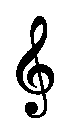
\includegraphics[height=14pt]{chapters/cap-musica-basica/G-clef.eps}. 
A posição donde esta clave se assine indica o lugar onde se localiza uma nota sol.
\begin{example}
Na Figura \ref{fig:abc-clavesol} podemos ver à clave de sol assinada sobre a segunda linha da pauta,
indicando que esta linha representa a nota sol.
\end{example} 
\item [Clave de fá:] Representada pelo símbolo 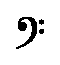
\includegraphics[height=10pt]{chapters/cap-musica-basica/FClef.eps}. 
A posição donde essa clave se assine indica o lugar onde se localiza uma nota fá.
\begin{example}
Na Figura \ref{fig:abc-clavefa} podemos ver à clave de fá assinada sobre a quarta linha da pauta,
indicando que essa linha representa a nota fá.
\end{example} 
\item [Clave de dó:] Representada pelo símbolo 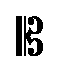
\includegraphics[height=10pt]{chapters/cap-musica-basica/CClef.eps}.
A posição donde esta clave se assine indica o lugar onde se localiza uma nota dó.
\begin{example}
Na Figura \ref{fig:abc-clavedo} podemos ver à clave de dó assinada sobre a terceira linha da pauta,
indicando que essa linha representa a nota dó.
\end{example} 
\end{description}
%%%
\begin{figure}[h]
    \centering
\begin{subfigure}[c]{0.25\textwidth}
\begin{abc}[name=abc-clavesol]
% abcm2ps clavesol.abc  -O clavesol.ps
% ps2epsi clavesol.ps clavesol.eps
%
X: 1 % start of header
K: C stafflines=5 %K: C %% Escala de C mayor %
M: none % M: 2/4
%T: Contratempo num compasso binário
V:1 clef=treble %name="Pauta com clave de sol"   sname="Pauta com clave de sol"
%
[V:1] G8
\end{abc}
\caption{Clave de sol com uma semibreve colocada em sol.}
\label{fig:abc-clavesol}
\end{subfigure}
~ %
\begin{subfigure}[c]{0.25\textwidth}
\begin{abc}[name=abc-clavefa]
% abcm2ps clavesfa.abc  -O clavefa.ps
% ps2epsi clavefa.ps clavefa.eps
%
X: 1 % start of header
K: C stafflines=5 %K: C %% Escala de C mayor %
M: none % M: 2/4
%T: Contratempo num compasso binário
V:1 clef=bass %name="Pauta com clave de fá"   sname="Pauta com clave de fá"
%
[V:1] F,8  
\end{abc}
\caption{Clave de fá com uma semibreve colocada em fá.}
\label{fig:abc-clavefa}
\end{subfigure}
~ %
\begin{subfigure}[c]{0.25\textwidth}
\begin{abc}[name=abc-clavedo]
% abcm2ps clavesfa.abc  -O clavedo.ps
% ps2epsi clavedo.ps clavedo.eps
%
X: 1 % start of header
K: C stafflines=5 %K: C %% Escala de C mayor %
M: none % M: 2/4
%T: Contratempo num compasso binário
V:1 clef=C %name="Pauta com clave de fá"   sname="Pauta com clave de fá"
%
[V:1] C8 
\end{abc}
\caption{Clave de dó com uma semibreve colocada em dó.}
\label{fig:abc-clavedo}
\end{subfigure}
    \caption{Tipos de claves}\label{fig:allclaves}
\end{figure}



\subsubsection{As claves e a escala diatonica}
Conhecida as definições das claves, e da \hyperref[sec:pos:Diatonica]{\textbf{escala diatônica}}, 
podemos misturar estes dois conceitos para conhecer a posição de todas as notas na pauta
\cite[pp. 10]{cardoso1973curso} \cite[pp. 14]{medteoria}.

Por exemplo, as pautas desenhadas na Figura \ref{fig:allnotesclaves} 
contem duas duas oitavas cada uma, centradas em dó, e com notas escritas usando semibreves.
\begin{figure}[h]
    \centering
\begin{abc}[name=abc-clavenotessol]
% abcm2ps clavenotessol.abc  -O clavenotessol.ps
% ps2epsi clavenotessol.ps clavenotessol.eps
%
X: 1 % start of header
K: C stafflines=5 %K: C %% Escala de C mayor %
M: none % M: 2/4
%T: Contratempo num compasso binário
V:1 clef=treble %name="Pauta com clave de sol"   sname="Pauta com clave de sol"
%
[V:1] "dó"C,8 "ré"D,8 "mi"E,8 "fá"F,8  "sol"G,8 "lá"A,8 "si"B,8 "dó"C8 "ré"D8 "mi"E8 "fá"F8  "sol"G8 "lá"A8 "si"B8 "dó"C'8 
\end{abc}

\begin{abc}[name=abc-clavenotesfa]
% abcm2ps clavenotesfa.abc  -O clavenotesfa.ps
% ps2epsi clavenotesfa.ps clavenotesfa.eps
%
X: 1 % start of header
K: C stafflines=5 %K: C %% Escala de C mayor %
M: none % M: 2/4
%T: Contratempo num compasso binário
V:1 clef=bass %name="Pauta com clave de fá"   sname="Pauta com clave de fá"
%
[V:1] C,8 D,8 E,8 F,8 G,8 A,8 B,8 C8 D8 E8 F8 G8 A8 B8 C'8 
\end{abc}

\begin{abc}[name=abc-clavenotesdo]
% abcm2ps clavenotesfa.abc  -O clavenotesdo.ps
% ps2epsi clavenotesdo.ps clavenotesdo.eps
%
X: 1 % start of header
K: C stafflines=5 %K: C %% Escala de C mayor %
M: none % M: 2/4
%T: Contratempo num compasso binário
V:1 clef=C %name="Pauta com clave de fá"   sname="Pauta com clave de fá"
%
[V:1] C,8 D,8 E,8 F,8 G,8 A,8 B,8 C8 D8 E8 F8 G8 A8 B8 C'8 
\end{abc}
    \caption{Tipos de claves}\label{fig:allnotesclaves}
\end{figure}
Na pauta com clave de sol, 
se distingue como as notas da oitava mais alta estão bem posicionadas na pauta;
porem, as notas da oitava inferior precisam linhas adicionais para serem representadas,
o que dificultará ou não deixará muito elegante a leitura dos elementos na pauta.
Podemos ver um caso similar, pero ao contrario, com a pauta que usa uma clave de fá;
nela, as notas da primeira oitava estão comodamente representadas dentro da pauta;
porem, as da oitava superior precisam linhas adicionais.
Finalmente, a notas escritas usando a clave de dó, estão bem centradas,
para notas com alturas intermédias e só fica fora da pauta as duas notas mais aguda e as duas mais graves.

A primeira vista poderia parecer mais vantajosa a clave de do, 
porem isto acontece só porque a nota central que queremos representar é um dó,
teríamos uma vantagem similar na clave de sol, se usaremos uma nota central em si,
ou a vantagem a teríamos na clave de fá, se usaremos uma nota central em ré. 
Na prática, escolher entre
uma clave u outra dependerá da melodia que queiramos encaixar na pauta.
Porem existe uma combinação muito usada na musica para piano, 
que é usar uma clave de sol pra descrever as melodias a serem tocadas pela mão direita,
e usar uma clave de fá, para as que serão tocadas pela mão esquerda; 
isto é conveniente devido a que se olhamos o dó central nessas claves, 
na Figura \ref{fig:allnotesclaves}, 
poderemos observar que esta nota se sai das linhas da pauta, 
justo para entrar nas linhas da pauta da outra mão.

%%%%%%%%%%%%%%%%%%%%%%%%%%%%%%%%%%%%%%%%%%%%%%%%%%%%%%%%%%%%%%%%%%%%%%%%%%%%%%%%
%%%%%%%%%%%%%%%%%%%%%%%%%%%%%%%%%%%%%%%%%%%%%%%%%%%%%%%%%%%%%%%%%%%%%%%%%%%%%%%%
\subsection{\textcolor{green}{Pauta de percussão}}\index{Pauta!Pauta de Percussão}

Existem varias formas de representar as pautas para percussão, 
estas são diferenciadas do pentagrama, devido a que na percussão, 
na maioria dos casos não se tem controle da \hyperref[sec:pos:Duracion]{\textbf{duração}} do som;
e sim se tem, do momento em que este será executado. Em outros casos,
pode estar desabilitada a possibilidade de mudar a \hyperref[sec:pos:Altura]{\textbf{altura}} dos sons;
pelo que não se necessitam linhas pra representar estas alturas.
Assim, as pautas de percussão estarão optimizadas, em cada caso, 
para mostrar com simplicidade o ritmo que se deseja interpretar.

\subsubsection{A clave de percussão}
Também chamada \textbf{clave neutral} ou \textbf{clave de ritmos}, 
porque é usada por percussionistas, bateristas, 
ou usada para qualquer instrumento que produz um som que não tem uma altura definida \cite[pp. 51]{harnum2009basic}.
Asim, esta clave indica que a pauta mostra ritmos e modos de tocar um instrumento, 
e não indica as alturas das notas, 
como outras claves mostradas na Seção \ref{subsubsec:clavespauta}.
Podemos achar dois símbolos equivalentes para representar esta clave, 
estes são \includegraphics[height=10pt]{chapters/cap-musica-basica/P1-clef.eps}
e \includegraphics[height=10pt]{chapters/cap-musica-basica/P2-clef.eps}.
Entre os instrumentos que usam esta clave temos:
o tambourine, o triangulo, o pandeiro, etc.
A Figura \ref{fig:allpercusionclaves} mostra algumas formas de usar a clave de percussão,
sendo formas equivalentes, as mostradas na Figura \ref{fig:abc-claveperczero} e a Figura \ref{fig:abc-clavepercuma}.

\begin{figure}[h]
    \centering 
\begin{subfigure}[c]{0.24\textwidth}
\begin{abc}[name=abc-clavepercusion1]
% abcm2ps clavepercusion1.abc  -O clavepercusion1.ps
% ps2epsi clavepercusion1.ps clavepercusion1.eps
%
X: 1 % start of header
K: C stafflines=0 %K: C %% Escala de C mayor %
M: none % M: 2/4
%T: Contratempo num compasso binário
V:1 clef=perc stem=up %name="Pauta com clave de fá"   sname="Pauta com clave de fá"
%
[V:1] B1 B1 B2 B1 B2   
\end{abc}
\caption{Clave de percussão sem linhas, indicando que só existe um modo de tocar o instrumento.}
\label{fig:abc-claveperczero}
\end{subfigure}
~%
\begin{subfigure}[c]{0.24\textwidth}
\begin{abc}[name=abc-clavepercusion2a]
% abcm2ps clavepercusion2a.abc  -O clavepercusion2a.ps
% ps2epsi clavepercusion2a.ps clavepercusion2a.eps
%
X: 1 % start of header
K: C stafflines=1 %K: C %% Escala de C mayor %
M: none % M: 2/4
%T: Contratempo num compasso binário
V:1 clef=perc stem=up %name="Pauta com clave de fá"   sname="Pauta com clave de fá"
%
[V:1] B1 B1 B2 B1 B2   
\end{abc}
\caption{Clave de percussão com uma linha e só um modo de tocar o instrumento.}
\label{fig:abc-clavepercuma}
\end{subfigure}
~%
\begin{subfigure}[c]{0.24\textwidth}
\begin{abc}[name=abc-clavepercusion2]
% abcm2ps clavepercusion2.abc  -O clavepercusion2.ps
% ps2epsi clavepercusion2.ps clavepercusion2.eps
%
X: 1 % start of header
K: C stafflines=1 %K: C %% Escala de C mayor %
M: none % M: 2/4
%T: Contratempo num compasso binário
V:1 clef=perc stem=up %name="Pauta com clave de fá"   sname="Pauta com clave de fá"
%
[V:1] A1 C'1 A2 C'1 A2   
\end{abc}
\caption{Clave de percussão com uma linha e dois modos de tocar o instrumento.}
\label{fig:abc-clavepercum2}
\end{subfigure}
~%
\begin{subfigure}[c]{0.24\textwidth}
\begin{abc}[name=abc-clavepercusion3]
% abcm2ps clavepercusion3.abc  -O clavepercusion3.ps
% ps2epsi clavepercusion3.ps clavepercusion3.eps
%
X: 1 % start of header
K: C stafflines=5 %K: C %% Escala de C mayor %
M: none % M: 2/4
%T: Contratempo num compasso binário
V:1 clef=perc stem=up %name="Pauta com clave de fá"   sname="Pauta com clave de fá"
%
[V:1] A1 B1 G2 C'1 F2   
\end{abc}
\caption{Clave de percussão com cinco linhas e vários modos de tocar o instrumento.}
\label{fig:abc-claveperccinco}
\end{subfigure}
    \caption{Usos da clave de percussão}\label{fig:allpercusionclaves}
\end{figure}

\subsubsection{O sistema de notação monolinear}
Este sistema foi criado pelo baterista suiço, Dr. Fritz Berger, em 1928. 
Ele o chamou ``the monolinear notation system'', 
de modo que seu sistema utilizava uma única linha na pauta, na sua definição,
a parte de acima da linha representava a mão direita (para bateria), e
a parte de abaixo da linha a mão esquerda.
Assim, era mais fácil ler os ritmos, deixando claro que mão devia fazer uma determinada ação
\cite[pp. 148]{beck1995encyclopedia} \cite[pp. 332]{dean2012drum}.
Um exemplo deste sistema pode ser visto na Figura \ref{fig:abc-clavepercum2}.

\subsubsection{The grid notation}


\cite[pp. 289]{gould676behind}

\begin{comment}
\subsubsection{The musical notation of percusion}
Revisar  \cite[pp. 70]{harnum2009basic}

Figura \ref{fig:abc-musicalperc}
\begin{figure}[H]
\centering
\begin{abc}[name=abc-musicalperc]
% abcm2ps musicalperc.abc  -O musicalperc.ps
% ps2epsi musicalperc.ps musicalperc.eps
%
X:1
T:Drum Key
M:
L:1/4
K:C clef=perc
"^Bass"F|"^Snare"c|"^High tom"e|"^Mid tom"d|"^Low tom"B|"^Floor tom"A|
"^Cymbal"^b|"^Crash"^a|"^Hi-hat"^g|"^Ride"^f|"^Hi-hat Pedal"^D|]

\end{abc}
\caption{Figuras e pausas}
\label{fig:abc-musicalperc}
\end{figure}
\end{comment}



%%%%%%%%%%%%%%%%%%%%%%%%%%%%%%%%%%%%%%%%%%%%%%%%%%%%%%%%%%%%%%%%%%%%%%%%%%%%%%%%

%%%%%%%%%%%%%%%%%%%%%%%%%%%%%%%%%%%%%%%%%%%%%%%%%%%%%%%%%%%%%%%%%%%%%%%%%%
\section{Intervalo melódico}
\label{sec:intervalomelodico}
\index{Música!Intervalo}
\index{Música!Intervalo melódico}


Um intervalo é a distância que existe entre dois sons de alturas definidas;
os intervalos melódicos correspondem à medição de notas musicais executadas uma após outra, 
numa melodia \cite[pp. 17]{holst1998abc}.
Assim, podem existir intervalos melódicos ascendentes ou descendentes,
que indicam que o tom da nota posterior é mais agudo ou mais grave, respetivamente \cite[pp. 17]{holst1998abc}.

Sobre a unidade de medição que será usada para quantificar as distancias nos intervalos, 
estes podem ser medidos usando sua posição relativa seguindo as sete notas da escala diatônica \cite[pp. 17]{holst1998abc}.
Por exemplo na Tabela \ref{tab:intervalomelodico} podemos ver os nomes usados seguindo esta notação.  
\begin{table}[h]
  \centering
  \begin{tabular}{|l|l||l|l|}
  \hline
  Intervalo & Posição     & Intervalo & Posição \\ \hline \hline
  Uníssono  & 1$^{\circ}$ & Segunda   & 2$^{\circ}$ \\ \hline
  Terça     & 3$^{\circ}$ & Quarta    & 4$^{\circ}$ \\ \hline
  Quinta    & 5$^{\circ}$ & Sexta     & 6$^{\circ}$ \\ \hline
  Sétima    & 7$^{\circ}$ & Oitava    & 8$^{\circ}$ \\ \hline
  \end{tabular}
  \caption{Distancia entre intervalos.}
  \label{tab:intervalomelodico}
\end{table}

Na Figura \ref{fig:abc-isegunda1} podemos ver um intervalo de uma segunda ascendente,
desde um dó ate um ré (+2 semitons).
Na Figura \ref{fig:abc-isegunda2} podemos ver um intervalo de uma segunda descendente,
desde um fá ate um mi (-1 semitons).
\begin{figure}[H]
    \centering
    \begin{subfigure}[b]{0.4\textwidth}
\begin{abc}[name=abc-isegunda1]
X: 1 % start of header
K: C % scale: C major
V:1 %name="Pauta com clave de fá"   sname="Pauta com clave de fá"
[V:1]  C2 D2
w: ~1º ~2º
\end{abc}
\caption{Intervalo de uma segunda ascendente.}
\label{fig:abc-isegunda1}
    \end{subfigure}
    \quad%~%add desired spacing between images, e. g. ~, \quad, \qquad, \hfill etc. 
      %(or a blank line to force the subfigure onto a new line)
    \begin{subfigure}[b]{0.4\textwidth}
\begin{abc}[name=abc-isegunda2]
X: 1 % start of header
K: C % scale: C major
V:1 %name="Pauta com clave de fá"   sname="Pauta com clave de fá"
[V:1]  F2 E2
w: ~1º ~2º
\end{abc}
\caption{Intervalo de uma segunda descendente.}
\label{fig:abc-isegunda2}
    \end{subfigure}
    \caption{Intervalo melódico de uma segunda.}
    \label{fig:intervalosegunda}
\end{figure}


Na Figura \ref{fig:abc-iterca1} podemos ver um intervalo de uma terça ascendente,
desde um fá ate um lá (+4 semitons).
Na Figura \ref{fig:abc-iterca2} podemos ver um intervalo de uma terça descendente,
desde um dó ate um lá (-3 semitons) \cite[pp. 16-17]{holst1998abc}.
\begin{figure}[H]
    \centering
    \begin{subfigure}[b]{0.4\textwidth}
\begin{abc}[name=abc-iterca1]
X: 1 % start of header
K: C % scale: C major
V:1 %name="Pauta com clave de fá"   sname="Pauta com clave de fá"
[V:1]  F2 A2
w: ~1º ~3º
\end{abc}
\caption{Intervalo de uma terça ascendente.}
\label{fig:abc-iterca1}
    \end{subfigure}
    \quad%~%add desired spacing between images, e. g. ~, \quad, \qquad, \hfill etc. 
      %(or a blank line to force the subfigure onto a new line)
    \begin{subfigure}[b]{0.4\textwidth}
\begin{abc}[name=abc-iterca2]
X: 1 % start of header
K: C % scale: C major
V:1 %name="Pauta com clave de fá"   sname="Pauta com clave de fá"
[V:1]  |C'2 A2|
w: ~1º ~3º
\end{abc}
\caption{Intervalo de uma terça descendente.}
\label{fig:abc-iterca2}
    \end{subfigure}
    \caption{Intervalo melódico de uma terça.}
    \label{fig:intervaloterca}
\end{figure}



Na Figura \ref{fig:abc-iquarta1} podemos ver um intervalo de uma quarta ascendente,
desde um sol ate um dó (+5 semitons) \cite[pp. 17]{holst1998abc}.
Na Figura \ref{fig:abc-iquarta2} podemos ver um intervalo de uma quarta descendente,
desde um sol ate um ré (-5 semitons).
\begin{figure}[H]
    \centering
    \begin{subfigure}[b]{0.4\textwidth}
\begin{abc}[name=abc-iquarta1]
X: 1 % start of header
K: C % scale: C major
V:1 %name="Pauta com clave de fá"   sname="Pauta com clave de fá"
[V:1]  G2 C'2
w: ~1º ~4º
\end{abc}
\caption{Intervalo de uma quarta ascendente.}
\label{fig:abc-iquarta1}
    \end{subfigure}
    \quad%~%add desired spacing between images, e. g. ~, \quad, \qquad, \hfill etc. 
      %(or a blank line to force the subfigure onto a new line)
    \begin{subfigure}[b]{0.4\textwidth}
\begin{abc}[name=abc-iquarta2]
X: 1 % start of header
K: C % scale: C major
V:1 %name="Pauta com clave de fá"   sname="Pauta com clave de fá"
[V:1]  G2 D2
w: ~1º ~4º
\end{abc}
\caption{Intervalo de uma quarta descendente.}
\label{fig:abc-iquarta2}
    \end{subfigure}
    \caption{Intervalo melódico de uma quarta.}
    \label{fig:intervaloquarta}
\end{figure}

Na Figura \ref{fig:abc-iquinta1} podemos ver um intervalo de uma quinta ascendente,
desde um si ate um fá (+6 semitons).
Na Figura \ref{fig:abc-iquinta2} podemos ver um intervalo de uma quinta descendente,
desde um dó ate um fá (-7 semitons) \cite[pp. 17]{holst1998abc}.
\begin{figure}[H]
    \centering
    \begin{subfigure}[b]{0.4\textwidth}
\begin{abc}[name=abc-iquinta1]
X: 1 % start of header
K: C % scale: C major
V:1 %name="Pauta com clave de fá"   sname="Pauta com clave de fá"
[V:1]  B,2 F2
w: ~1º ~5º
\end{abc}
\caption{Intervalo de uma quinta ascendente.}
\label{fig:abc-iquinta1}
    \end{subfigure}
    \quad%~%add desired spacing between images, e. g. ~, \quad, \qquad, \hfill etc. 
      %(or a blank line to force the subfigure onto a new line)
    \begin{subfigure}[b]{0.4\textwidth}
\begin{abc}[name=abc-iquinta2]
X: 1 % start of header
K: C % scale: C major
V:1 %name="Pauta com clave de fá"   sname="Pauta com clave de fá"
[V:1]  C'2 F2
w: ~1º ~5º
\end{abc}
\caption{Intervalo de uma quinta descendente.}
\label{fig:abc-iquinta2}
    \end{subfigure}
    \caption{Intervalo melódico de uma quinta.}
    \label{fig:intervaloquinta}
\end{figure}

Na Figura \ref{fig:abc-isexta1} podemos ver um intervalo de uma sexta ascendente,
desde um dó ate um lá (+9 semitons).
Na Figura \ref{fig:abc-isexta2} podemos ver um intervalo de uma sexta descendente,
desde um mi ate um sol (-9 semitons) \cite[pp. 18]{holst1998abc}.
\begin{figure}[H]
    \centering
    \begin{subfigure}[b]{0.4\textwidth}
\begin{abc}[name=abc-isexta1]
X: 1 % start of header
K: C % scale: C major
V:1 %name="Pauta com clave de fá"   sname="Pauta com clave de fá"
[V:1]  C2 A2
w: ~1º ~6º
\end{abc}
\caption{Intervalo de uma sexta ascendente.}
\label{fig:abc-isexta1}
    \end{subfigure}
    \quad%~%add desired spacing between images, e. g. ~, \quad, \qquad, \hfill etc. 
      %(or a blank line to force the subfigure onto a new line)
    \begin{subfigure}[b]{0.4\textwidth}
\begin{abc}[name=abc-isexta2]
X: 1 % start of header
K: C % scale: C major
V:1 %name="Pauta com clave de fá"   sname="Pauta com clave de fá"
[V:1]  E'2 G2
w: ~1º ~6º
\end{abc}
\caption{Intervalo de uma sexta descendente.}
\label{fig:abc-isexta2}
    \end{subfigure}
    \caption{Intervalo melódico de uma sexta.}
    \label{fig:intervalosexta}
\end{figure}

Na Figura \ref{fig:abc-isetima1} podemos ver um intervalo de uma sétima ascendente,
desde um ré ate um dó (+10 semitons) \cite[pp. 18]{holst1998abc}.
Na Figura \ref{fig:abc-isetima2} podemos ver um intervalo de uma sétima descendente,
desde um si ate um dó (-11 semitons).
\begin{figure}[H]
    \centering
    \begin{subfigure}[b]{0.4\textwidth}
\begin{abc}[name=abc-isetima1]
X: 1 % start of header
K: C % scale: C major
V:1 %name="Pauta com clave de fá"   sname="Pauta com clave de fá"
[V:1]  D2 C'2
w: ~1º ~7º
\end{abc}
\caption{Intervalo de uma sétima ascendente.}
\label{fig:abc-isetima1}
    \end{subfigure}
    \quad%~%add desired spacing between images, e. g. ~, \quad, \qquad, \hfill etc. 
      %(or a blank line to force the subfigure onto a new line)
    \begin{subfigure}[b]{0.4\textwidth}
\begin{abc}[name=abc-isetima2]
X: 1 % start of header
K: C % scale: C major
V:1 %name="Pauta com clave de fá"   sname="Pauta com clave de fá"
[V:1]  E'2 G2
w: ~1º ~7º
\end{abc}
\caption{Intervalo de uma sétima descendente.}
\label{fig:abc-isetima2}
    \end{subfigure}
    \caption{Intervalo melódico de uma sétima.}
    \label{fig:intervalosetima}
\end{figure}

%%%%%%%%%%%%%%%%%%%%%%%%%%%%%%%%%%%%%%%%%%%%%%%%%%%%%%%%%%%%%%%%%%%%%%%%%%%%%%%%
\subsection{Qualidade do intervalo}
Além do uso de notas musicais para quantificar o intervalo, 
estos também podem ter uma qualificação,
os intervalos de 4$^{\circ}$, 5$^{\circ}$ e 8$^{\circ}$ são chamados justos,
e os intervalos 2$^{\circ}$, 3$^{\circ}$, 6$^{\circ}$  e 7$^{\circ}$ são chamados maiores \cite[pp. 19]{bennett1993elementos}.

A Figura \ref{fig:justo-maior} mostra as possibilidades que podem tomar as qualificações.
\begin{figure}[h]
  \centering
    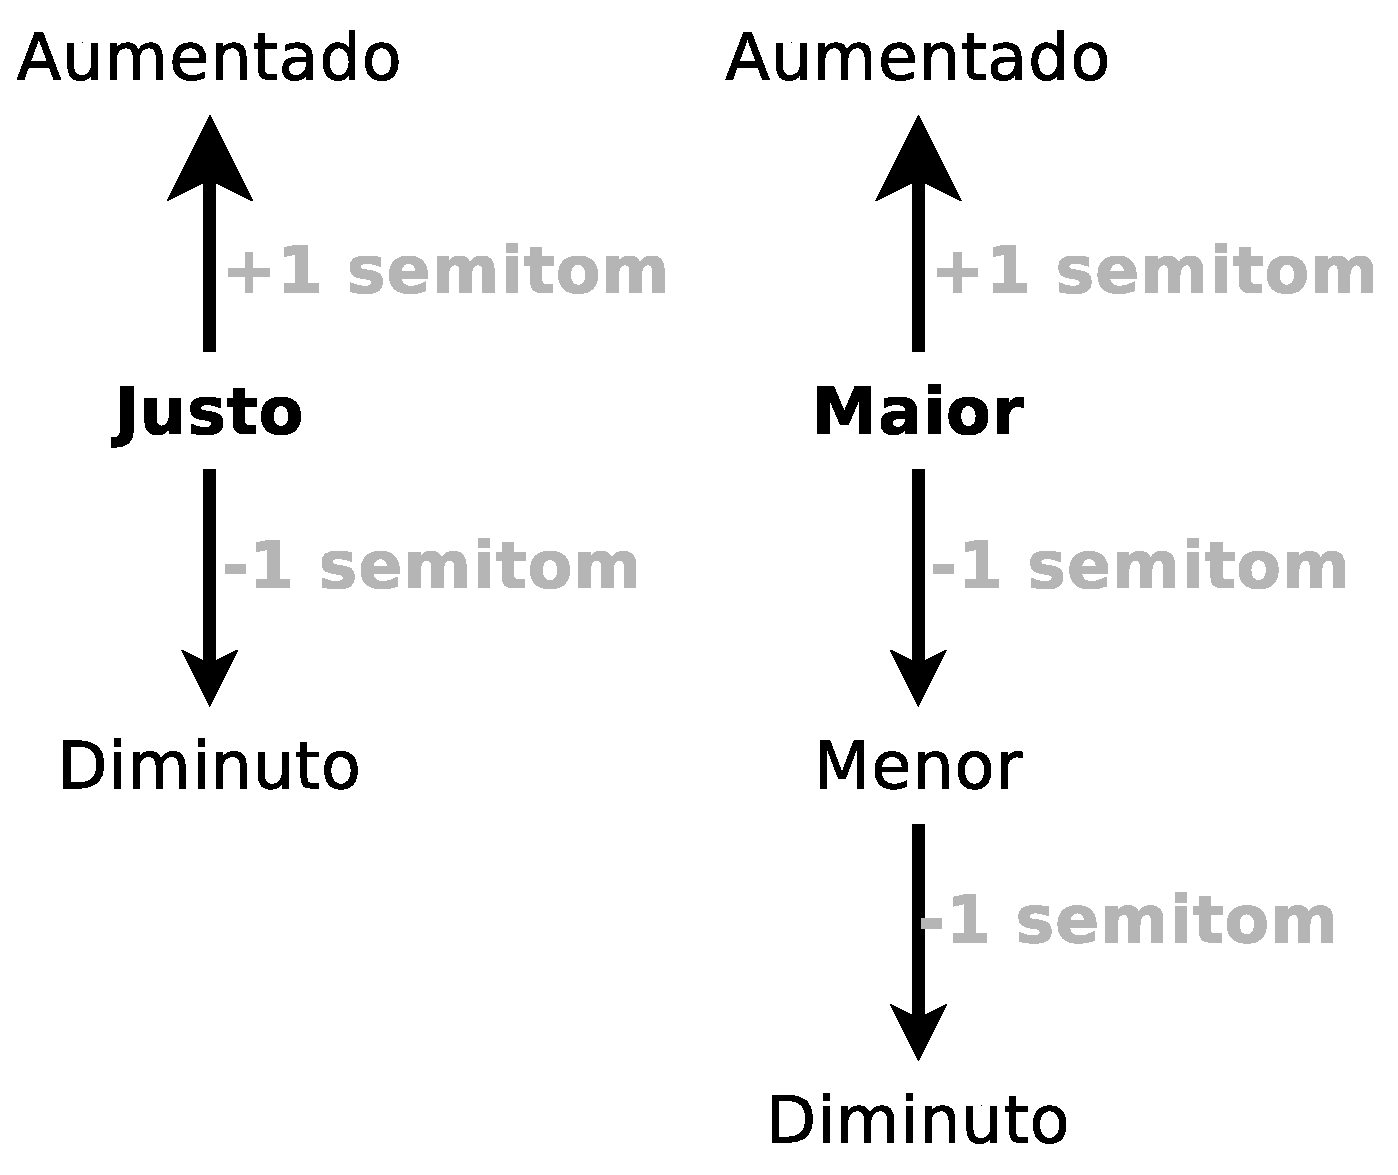
\includegraphics[width=0.5\textwidth]{chapters/cap-musica-basica/justo-maior.eps}
  \caption{Intervalos justos maiores e menores.}
  \label{fig:justo-maior}
\end{figure}
Uma forma rápida de lembrar os nomes é seguindo a escala em dó maior, como 
na Figura \ref{fig:abc-justo-maior2}, onde M indica maior e J indica justo. 
\begin{figure}[H]
    \centering
\begin{abc}[name=abc-justo-maior2]
X: 1 % start of header
K: C % scale: C major
V:1 %name="Pauta com clave de fá"   sname="Pauta com clave de fá"
[V:1]  C8 D8 E8 F8 G8 A8 B8 C'8
w:     ~1ºJ ~2ºM ~3ºM ~4ºJ ~5ºJ ~6ºM ~7ºM ~8ºJ
\end{abc}
\caption{Intervalo de uma sétima descendente.}
\label{fig:abc-justo-maior2}
\end{figure}



A Tabela \ref{tab:intervalomelodico2} mostra o número de semitons 
correspondente a cada intervalo \cite[pp. 89-90]{cardoso1973curso} \cite[pp. 72-74]{holst1998abc}.

\begin{table}[h]
  \centering
  \begin{tabular}{|l|l|l|l|}
  \hline
  \textbf{Intervalo} & \textbf{Semitons} & \textbf{Tons} & \textbf{Exemplo}     \\ \hline \hline
  ~                & 0        & 0        & dó \\ \hline
  Segunda menor    & 1        & 1/2      & ré$\flat$ \\ \hline
  Segunda maior    & 2        & 1        & ré        \\ \hline  \hline
  Terça menor      & 3        & 1+1/2    & mi$\flat$ \\ \hline
  Terça maior      & 4        & 2        & mi        \\ \hline  \hline
  \textbf{Quarta justa}     & \textbf{5}        & \textbf{2+1/2}    & \textbf{fá}        \\ \hline
  Quarta aumentada & 6        & 3        & fá$\#$    \\ \hline \hline
  Quinta diminuta  & 6        & 3        & sol$\flat$ \\ \hline 
  \textbf{Quinta justa}     & \textbf{7}        & \textbf{3+1/2}    & \textbf{sol}      \\ \hline \hline
  Sexta menor      & 8        & 4        & lá$\flat$ \\ \hline
  Sexta maior      & 9        & 4+1/2    & lá        \\ \hline \hline
  Sétima menor     & 10       & 5        & si$\flat$ \\ \hline
  Sétima maior     & 11       & 5+1/2    & si        \\ \hline \hline
  \textbf{Oitava justa}     & 12       & 6        & \textbf{dó} \\ \hline
  \end{tabular}
  \caption{Distancia entre intervalos.}
  \label{tab:intervalomelodico2}
\end{table}
         
%%%%%%%%%%%%%%%%%%%%%%%%%%%%%%%%%%%%%%%%%%%%%%%%%%%%%%%%%%%%%%%%%%%%%%%%%%%%%%%%
\section{\textcolor{green}{Compasso}}\index{Compasso}
\label{sec:compaso}

\begin{description}
\item[Compasso:] O dicionário de Harvard de música \cite[pp. 513]{apel1969harvard} define compasso (``measure'' em inglês)
como um grupo de tempos, batimentos ou pulsos (unidade do tempo musical),
onde o primeiro destes normalmente é acentuado. 
Este número de tempos no compasso pode ser, dois, trés, quatro, ou ocasionalmente 5 ou mais. 
Sendo estos compassos separados por barras verticais e as notas do compasso esquematizados baixo uma métrica.
\begin{example}
Figura \ref{fig:abc-exemplocompasso1}
\end{example}
 
\item[Métrica:] Sobre a métrica  (``meter'' em inglês) o dicionario \cite[pp. 523]{apel1969harvard} explica que é
um padrão de unidades temporais fixas, chamados batimentos, 
pelo qual um período de tempo de uma peça musical ou uma seção dela é medida. 
Agrega tambem que a métrica é indicado geralmente por uma fração, como por exemplo:
${2}/{2}$ , ${3}/{4}$ , ${4}/{4}$, etc. Em português esta fração é chamada de formula do compasso. 
\begin{example}
Figura \ref{fig:abc-exemplocompasso1}
\end{example}
\end{description}

O numerador, da formula do compasso, indica o número de pulsações (tempos) que compõem cada compasso.
Por outro lado o denominador nos informa al longitude temporal de cada um dos tempos do compasso.

\begin{figure}[h]
\centering
\begin{abc}[name=abc-exemplocompasso1]
% abcm2ps exemplocompasso1.abc  -O exemplocompasso1.ps
% ps2epsi exemplocompasso1.ps exemplocompasso1.eps
%
X: 1 % start of header
K: none stafflines=0 %K: C %% Escala de C mayor %
M: 2/4
%T: Contratempo num compasso binário
V:1 clef=perc stem=up name="Ritmo 1"   sname="Ritmo 1"
%
[V:1] | B2 B1 B1| B2 B1 B1 | B2 B1 B1 | B2 z2  |
%       
\end{abc}
\caption{Figuras e pausas}
\label{fig:abc-exemplocompasso1}
\end{figure}



A Tabela \ref{tab:abc-noteslength} exemplifica o significado do denominador da formula do compasso; 
\begin{table}[h]
\centering
\begin{tabular}{|c|c|c|c|}
\hline
denominador & Figura  & Duração & Nome\\ \hline
\hline
$1$   & \fullnote    & $S$   & Semibreve \\ \hline
$2$ & \halfnote    & $S/2$ & Mínima \\ \hline
$4$ & \quarternote & $S/4$ & Semínima \\ \hline
$8$ & \eighthnote  & $S/8$ & Colcheia \\ \hline
\end{tabular}
\caption{Duração e símbolos de algumas figuras musicais}
\label{tab:abc-noteslength}
\end{table}
onde a primeira coluna mostra o denominador da formula,
a segunda coluna mostra as figuras musicais que representam cada um dos tempos do compasso, e 
a terceira e quarta coluna, indicam a duração em segundos e o nome da figura musical.

podemos achar equivalências aos exemplos da formula do compasso dados
anteriormente; onde os compassos com formula $\mathbf{2}/2$ tem cada um, uma duração de $\mathbf{2}$\halfnote ~(duas mínimas),  
compassos com formula $\mathbf{3}/4$ tem uma duração de $\mathbf{3}$\quarternote ~(trés semínimas) 
e $\mathbf{4}/4$ uma duração de $\mathbf{4}$\quarternote ~(quatro semínimas). É importante
ressaltar que a duração em tempo das figuras musicais é relativa, como pode ser visto
na terceira coluna da Tabela \ref{tab:abc-noteslength}, onde as durações estão em função
da duração $S$ da semibreve. 


Se classificamos os compassos por sua métrica, os três tipos mais conhecidos 
são os compassos binários, ternários, quaternários \cite[pp. 27]{adolfo2002musica}.

\subsection{\textcolor{green}{Compasso binário}}\index{Compasso!Compasso Binário} Ou compasso binário simples,
é uma estrutura rítmica que se carateriza por ter compassos com uma  duração de dois tempos,
sendo o primeiro tempo forte (acentuado), e o segundo de tempo fraco (não acentuado)
\cite[pp. 41]{grabner2001teoria} \cite[pp. 66]{adolfo2002musica}\cite[pp. 28]{alves2004teoria}. 
Os compassos binários (simples) tem uma formula de compasso na forma $2/B$,
onde $B$ pode ser $2$, $4$, $8$, etc. 
A Figura \ref{compasso:binario}, representa um exemplo de compasso binário simples, 
com formula de compasso $2/2 \equiv 2$\halfnote, 
e tempos com uma duração de $S/2$ (uma \halfnote), 
sendo que o primeiro compasso contem $2$\halfnote~e o segundo contem $4$\quarternote.
Na Figura \ref{compasso:binario} a sigla ``N.A.'' significa ``Não acentuado'', pelo que é fácil perceber
que em qualquer caso, só a nota que é executada no tempo 1 é acentuada.
\begin{figure}[H]
\centering
\begin{abc}[name=abc-compasso1]
X: 1 % start of header
K: C % scale: C major
M: 2/2 %meter - compasso
"Primeiro compasso" G4 F4 |"Segundo compasso" G2 D2 F2 D2  |
w: Acentuado N.A. Acentuado N.A. N.A. N.A.
\end{abc}
\caption{Exemplo de compasso binário (simples)}
\label{compasso:binario}
\end{figure}

Se falamos de forma mais geral, 
podemos ter dois tipos de compassos binários: os simples e os compostos.
Assim, 
para achar a formula de um compasso composto, correspondente a um compasso simples (usando quialteras de três)
usamos a seguinte operação \cite[pp. 74]{alves2004teoria}, 
\begin{equation}\label{eq:comcomposto}
Compasso~simples\times\frac{3}{2}=Compasso~composto.
\end{equation}
De modo que obtemos compassos binários compostos com as seguintes formulas de compasso: 
$6/4$, $6/8$, $6/16$, etc.
A diferencia do visto nos compassos binários simples, os compassos binários compostos tem 
um pulso forte (Acentuado) no tempo 1 e um pulso semiforte (Acentuado porem menor) no tempo 4, 
de modo que os tempos 2,3,5 e 6,
são classificados como tempos fracos (Não Acentuados)\cite[pp. 41]{grabner2001teoria}.
A Figura \ref{compasso:binariocomposto}, representa um exemplo de compasso binário composto, 
com formula de compasso $6/4 \equiv 6$\quarternote, 
e tempos com uma duração de $S/4$ (uma \quarternote), 
sendo que o primeiro compasso contem $6$\quarternote~e o segundo contem dois $2$\quarternote~e dois $2$\halfnote.
Da Figura \ref{compasso:binariocomposto} é fácil perceber
que em qualquer caso, só são acentuados as nota que são executadas no tempo 1 e 4; 
aclarando que as notas executadas no tempo 4 tem uma acentuação menor que as executadas no tempo 1.
\begin{figure}[H]
\centering
\begin{abc}[name=abc-compasso1c]
X: 1 % start of header
K: C % scale: C major
M: 6/4 %meter - compasso
"Primeiro compasso" G2 D2 D2 F2 D2 D2 |"Segundo compasso" G2 D4 F2 D4  |
w: Acentuado N.A. N.A. Acentuado N.A N.A. Acentuado N.A. Acentuado N.A. 
\end{abc}
\caption{Exemplo de compasso binário composto}
\label{compasso:binariocomposto}
\end{figure}

Alguns autores consideram aos compassos quaternários (ex: 4/4, 4/8) como um caso de compasso binário,
chamando eles de compasso binário duplo \cite[pp. 41]{grabner2001teoria}.




\subsection{\textcolor{green}{Compasso ternário}}\index{Compasso!Compasso Ternário} Ou compasso ternário simples,
é uma estrutura rítmica que se carateriza por ter compassos com trés tempos,
sendo o primeiro pulso forte (acentuado) e os outros dois fracos (não acentuados) 
\cite[pp. 67]{adolfo2002musica}\cite[pp. 30]{alves2004teoria}. 
Os compassos ternários (simples) tem uma formula de compasso da forma $3/B$, 
onde $B$ pode ser $2$, $4$, $8$, etc.
Por exemplo temos, as formulas de compassos ternários simples: $3/2$, $3/4$, $3/8$,  etc.

A Figura \ref{compasso:ternario}, representa um exemplo de compasso ternário (simples), com 
formula de compasso $3/4 \equiv 3$\quarternote, 
onde os tempos tem uma duração de $S/4$, o primeiro compasso contem $3$\quarternote~e
o segundo contem $6$\eighthnote.
Na Figura \ref{compasso:ternario}  é fácil perceber
que em ambos compassos, só a nota que é executada no tempo 1 é acentuada.
\begin{figure}[H]
\centering
\begin{abc}[name=abc-compasso2]
X: 1 % start of header
K: C % scale: C major
M: 3/4 %meter - compasso
"Primeiro compasso" G2 F2 F2 |"Segundo compasso" G1 F1 E1 D1 D1  D1  |
w: Acentuado N.A. N.A. Acentuado N.A N.A.  N.A. N.A. N.A. 
\end{abc}
\caption{Exemplo de compasso ternário}
\label{compasso:ternario}
\end{figure}


São chamados de compassos ternários compostos,  
quando estes tem uma formula de compasso como: $9/4$, $9/8$ e $9/16$.
Para gerar estes compassos compostos a partir de suas versões simples,
se segue a mesma operação descrita na Equação \ref{eq:comcomposto}.


\subsection{\textcolor{green}{Compasso quaternário}}\index{Compasso!Compasso Quaternário} Ou compasso quaternário simples,
é uma estrutura rítmica que se carateriza por ter compassos com quatro tempos,
sendo o primeiro pulso forte (acentuado), o segundo fraco (não acentuado), 
o terceiro semiforte (acentuado porem menor) e o último fraco (não acentuado) 
\cite[pp. 67]{adolfo2002musica}\cite[pp. 32]{alves2004teoria}. 
Os compassos quaternários (simples) tem uma formula de compasso da forma $4/B$, 
onde $B$ pode ser $2$, $4$, $8$, etc.
Por exemplo temos, as formulas de compassos ternários simples: $4/2$, $4/4$, $4/8$,  etc.

A Figura \ref{compasso:quaternario}, representa um exemplo de compassos quaternário, com 
formula de compasso $4/4 \equiv 4$\quarternote, 
onde cada tempo tem uma duração de $S/4$, o primeiro compasso contem $4$\quarternote~e
o segundo contem $8$\eighthnote.
Na Figura \ref{compasso:ternario}  é fácil perceber
que em ambos compassos, só as notas que são executadas no tempo 1 e 3 são acentuadas.
\begin{figure}[H]
\centering
\begin{abc}[name=abc-compasso3]
X: 1 % start of header
K: C % scale: C major
M: 4/4 %meter - compasso
"Primeiro compasso" G2 D2 F2 D2|"Segundo compasso" G1 F1 D1 C1 F1 E1 D1 C1 |
w: Acentuado N.A. Acentuado N.A. Acentuado N.A N.A. N.A. Acentuado N.A. N.A. N.A. 
\end{abc}
\caption{Exemplo de compasso quaternário}
\label{compasso:quaternario}
\end{figure}

São chamados de compassos quaternários compostos,  
quando estes tem uma formula de compasso como: $12/4$, $12/8$ e $12/16$.
Para gerar estes compassos compostos a partir de suas versões simples,
se segue a mesma operação descrita na Equação \ref{eq:comcomposto}.
 

%%%%%%%%%%%%%%%%%%%%%%%%%%%%%%%%%%%%%%%%%%%%%%%%%%%%%%%%%%%%%%%%%%%%%%%%%%%%%%%%
\section{Andamento}
\index{Música!Andamento}
\label{sec:Andamento}

Como temos visto nos capítulos anteriores, 
as figuras musicais podem ser colocadas em alturas fixas (ex: Um lá a 440Hz);
porem ate agora a duração das figuras musicais numa melodia só foram medidas de forma relativas,
como foi visto na Tabela \ref{tab:abc-noteslengthbasic}.

Assim, é preciso indicar qualitativa ou quantitativamente aos interpretes,
qual será o valor de cada figura musical na melodia a executar;
pelo que é comum ver indicado no inicio da pauta o ``andamento'', 
com palavras como ``rápido'', ``moderado'' ou ``lento'' \cite[pp. 29]{holst1998abc} \cite[pp. 115]{mascarenhascurso};
pelo que se define o andamento como o grau de lentidão ou rapidez ao executar uma peça musical \cite[pp. 115]{mascarenhascurso}.

Se o compositor quer ser mais exato, 
também pode indicar o andamento de uma peça musical,
descrevendo quantas figuras musicais podem ser executadas por minuto;
por exemplo a indicação, \Vier=80, 
o que quer dizer que levaria um minuto para que 80 semínimas fossem executadas \cite[pp. 29]{holst1998abc};
um exemplo disto pode ser visto na Figura \ref{fig:andamento1}. 

\begin{figure}[!h]
\centering
\begin{abc}[name=abc-andamento1]
X: 1 % start of header
K: C stafflines=1 % scale: C major
M: 2/4 %meter - compasso
Q:1/4=80
V:1 clef=perc stem=up %name="Pauta com clave de fá"   sname="Pauta com clave de fá"
[V:1] |:!>!B3/2 B/2 B1 B1| B3/2 B/2 B1 B1 | B2 B2| B2 z2:|
\end{abc}
\caption{Frase rítmica com um andamento de \Vier=80.}
\label{fig:andamento1}
\end{figure}
 


%%%%%%%%%%%%%%%%%%%%%%%%%%%%%%%%%%%%%%%%%%%%%%%%%%%%%%%%%%%%%%%%%%%%%%%%%%%%%%%%

\section{Ligadura}
\index{Música!Ligadura}
\label{sec:ligadura}

A ligadura é uma linha curva que se coloca sobre duas ou mais notas da mesma altura, 
indicando que somente a primeira é articulada, 
e esta tem uma duração equivalente a soma de todas as notas ligadas \cite[pp. 35]{cardoso1973curso}.

\begin{example}
A Figura \ref{fig:total-ligadura} descreve 3 casos de uso de ligadura.
\begin{itemize}
\item Na Figura \ref{fig:abc-ligadura1} pode-se ver que, no primeiro compasso, 
tem-se uma ligadura entre a primeira e a segunda figura musical; 
no segundo compasso tem-se uma representação equivalente ao primeiro compasso; 
porém, usando ponto de aumento.
\item Na Figura \ref{fig:abc-ligadura2} pode-se ver que, no primeiro compasso, 
tem-se ligaduras entre as três primeiras figuras musicais; 
no segundo compasso tem-se uma representação equivalente ao primeiro compasso; 
porém, usando dois pontos de aumento.
\item Na Figura \ref{fig:abc-ligadura3} tem-se um exemplo de uso de ligadura entre figuras musicais de diferentes compassos,
de modo que a duração da última nota, do primeiro compasso, se prolonga até o segundo compasso.
\end{itemize}
\end{example}


\begin{figure}[!ht]
    \centering
    \begin{subfigure}[b]{0.6\textwidth}
\begin{abc}[name=abc-ligadura1]
X: 1 % start of header
K: C %% Escala de C mayor %
M: 2/4
%T: Contratempo num compasso binário
V:1 clef=G  %name="Ritmo 1"   sname="Ritmo 1"
%
[V:1] | (B2 B1) C1 | B3 C1   |    
\end{abc}
\vspace{-10pt}
\caption{Uso de ligaduras entre duas notas}
\label{fig:abc-ligadura1}
    \end{subfigure}
    ~%add desired spacing between images, e. g. ~, \quad, \qquad, \hfill etc. 
      %(or a blank line to force the subfigure onto a new line)
    \begin{subfigure}[b]{0.6\textwidth}
\begin{abc}[name=abc-ligadura2]
X: 1 % start of header
K: C %% Escala de C mayor %
M: 2/4
%T: Contratempo num compasso binário
V:1 clef=G  %name="Ritmo 1"   sname="Ritmo 1"
%
[V:1] | (A2 (A1) A1/2) C1/2 | A7/2 C1/2  |
\end{abc}
\vspace{-10pt}
\caption{Uso de ligaduras entre três notas.}
\label{fig:abc-ligadura2}
    \end{subfigure}
    ~%add desired spacing between images, e. g. ~, \quad, \qquad, \hfill etc. 
      %(or a blank line to force the subfigure onto a new line)
    \begin{subfigure}[b]{0.6\textwidth}
\begin{abc}[name=abc-ligadura3]
X: 1 % start of header
K: C %% Escala de C mayor %
M: 2/4
%T: Contratempo num compasso binário
V:1 clef=G  %name="Ritmo 1"   sname="Ritmo 1"
%
[V:1] | B3  (G1 | G2) B2  |
\end{abc}
\vspace{-10pt}
\caption{Uso de ligaduras em notas de compassos distintos.}
\label{fig:abc-ligadura3}
    \end{subfigure}
    \caption{Distintos usos da ligadura.}\label{fig:total-ligadura}
\end{figure}


%%%%%%%%%%%%%%%%%%%%%%%%%%%%%%%%%%%%%%%%%%%%%%%%%%%%%%%%%%%%%%%%%%%%%%%%%%%%%%%%
\section{Tempo}
\index{Tempo}
\label{sec:Tempo}

Como já foi sugerido na Seção \ref{sec:compaso}, é chamado de "tempo" 
à pulsação básica que é usada como unidade de medida das composições musicais.
Os tempos ao ser agrupados em compassos podem formar diferentes estruturas como por exemplo: 
\hyperref[subsec:compassobinario]{\textbf{compassos binários}}, \hyperref[subsec:compassoternario]{\textbf{ternários}} e \hyperref[subsec:compassoquaternario]{\textbf{quaternários}}; que tem uma duração de 2 tempos, 
3 tempos e 4 tempos, respetivamente. 

\begin{notation}[] Para o melhor entendimento das seguintes seções usaremos algumas notações.
\begin{itemize}
\item A variável $T$ será usada para designar à duração em segundos de cada tempo,
sendo que o valor de $T$ variará dependendo da formula do compasso usada.

\item As subdivisões dos tempos serão designadas com as seguintes variáveis:
\begin{itemize}
\item ``FF'' indica que é a parte forte de um tempo forte,
\item ``Ff'' indica que é a parte fraca de um tempo forte,
\item ``fF'' indica que é a parte forte de um tempo fraco,
\item ``ff'' indica que é a parte fraca de um tempo fraco.
\end{itemize}
\end{itemize}

\end{notation}

\subsection{Tempos fortes e fracos}
\index{Tempo!Tempo forte}
\index{Tempo!Tempo fraco}

A formula do compasso de uma peça musical ou uma porção dela, 
nos indica quantos tempos e que duração terão estes tempos no compasso; 
porem, além destas informações, 
a formula do compasso também nos indica o \hyperref[def:acentometrico]{\textbf{acento métrico}} \cite[pp. 70]{cardoso1973curso}; 
é dizer quias serão os tempos fortes, semifortes e fracos no compasso.


\begin{description}
\item[O acento métrico] \label{def:acentometrico} é constituído pelas acentuações fortes e fracas dos tempos dos compassos, 
os acentos métricos não precisam ser grafados na pauta \cite[pp. 141]{medteoria}.
\item[O tempo forte (F)] \label{def:tempoforte} sempre será o primeiro tempo de cada compasso. 
Um tempo forte não necessita uma grafia especial que indique que este deve ser articulado
com maior \hyperref[sec:pos:Intensidade]{\textbf{intensidade}}; é dizer, com acentuação.
\item[O tempo semiforte (sF)] \label{def:temposemiforte} acontece em alguns tipos de compasso, 
como nos compassos quaternários. 
Um tempo semiforte terá uma acentuação menor à do tempo forte, porem maior à de um tempo fraco. 
Este tempo não necessita uma grafia especial que indique que deve ser articulado
com \hyperref[sec:pos:Intensidade]{\textbf{intensidade}}.
\item[O tempo fraco (f)] \label{def:tempofraco} corresponde a todos os tempos que não sejam né fortes, né semifortes,
de modo que estes tempos não tem acentuação. 
\end{description}~

Uma versão mais simplificada das informações dadas anteriormente, 
pode ser vista na seguinte equação que mostra a relação de \hyperref[sec:pos:Intensidade]{\textbf{intensidades}}:
\begin{equation}
f ~<~ sF ~<~ F.
\end{equation}

Porem, 
se utilizamos as subdivisões de tempos, 
a relação de \hyperref[sec:pos:Intensidade]{\textbf{intensidades}} pode ser expressada mediante a seguinte equação:
\begin{equation}
\{fF=ff\} ~<~  \{f = fF\} ~<~ sF ~<~ \{F = FF\} 
\end{equation}

\begin{remark}
A regularidade na distribuição das acentuações nos tempos, 
só mudará quando se especifiquem  explicitamente dinâmicas sobre as figuras musicais,
de modo que estas dinâmicas modificam as acentuações,
porem não trocam o nome dos tempos, sendo estes sempre chamados de tempos fortes, semifortes e fracos. 
\end{remark}


\begin{example}
Na Figura \ref{fig:abc-tempo1} podemos ver 2 compassos com a mesma métrica, 
tendo eles uma formula de compasso 2/2; é dizer, 
cada compasso tem dois tempos, como uma duração de uma mínima (\halfnote) para cada tempo.
\begin{itemize}
\item O primeiro compasso é preenchido com duas notas que usam figuras musicais que duram um tempo cada um;
de modo que 
a primeira nota será executada no tempo forte, 
possuindo esta nota um \hyperref[def:acentoprincipal]{\textbf{acento  principal}}, e 
a segunda nota é executada no tempo fraco e não leva acento; 
é dizer tem um menor \hyperref[sec:pos:Intensidade]{\textbf{intensidade}} que a nota do primeiro tempo.
\item No segundo compasso, este é preenchido com 4 notas que usam figuras musicais que duram 1/2 tempo cada uma;
Assim, 
\begin{itemize}
\item a primeira nota será executada em FF (acentuada como F),
\item a segunda  nota será executada em Ff (menos acentuada que f),
\item a terceira nota será executada em fF (acentuada como f), e 
\item a quarta   nota será executada em ff (menos acentuada que f).
\end{itemize}
\end{itemize} 
\end{example}
\begin{figure}[H]
\centering
\begin{abc}[name=abc-tempo1,width=0.6\linewidth]
X: 1 % start of header
K: none stafflines=0 %K: C %% Escala de C mayor %
M: 2/2 %meter - compasso
V:1 clef=perc stem=up name="Ritmo"   sname="Ritmo"
[V:1] | B4 B4 |  B2 B2 B2 B2 |  
w:  T T    T/2 T/2 T/2 T/2 
w:  F f FF Ff fF ff
\end{abc}
\caption{Dois compassos com 2 tempos cada um.}
\label{fig:abc-tempo1}
\end{figure}


\begin{example}
Na Figura \ref{fig:abc-tempo2} podemos ver 2 compassos com a mesma métrica, 
tendo eles uma formula de compasso 4/4; é dizer, 
cada compasso tem quatro tempos, como uma duração de uma semínima (\quarternote) para cada tempo.
\begin{itemize}
\item O primeiro compasso é preenchido com duas notas que usam figuras musicais que duram dois tempos cada um;
de modo que a primeira nota será executada no tempo forte,
possuindo esta nota um \hyperref[def:acentoprincipal]{\textbf{acento  principal}}, 
e o som será sustenido ate completar o seguinte tempo fraco, 
a segunda nota será executada no tempo semiforte,
possuindo esta nota um \hyperref[def:acentosecundario]{\textbf{acento  secundario}},
 e o som será sustenido ate completar o seguinte tempo fraco.
Em ambas figuras não são colocados os símbolos, F e sF, 
pois as notas ocupam mais de um tempo, porem as acentuações são respeitadas.
\item O segundo compasso é preenchido com 4 notas que usam figuras musicais que duram 1 tempo cada uma;
Assim, 
a primeira nota será executada no tempo forte (F),
a segunda  nota será executada no tempo fraco (f),
a terceira nota será executada no tempo semiforte (sF), e 
a quarta   nota será executada no tempo fraco (f).
\end{itemize} 
\end{example}
\begin{figure}[H]
\centering
\begin{abc}[name=abc-tempo2,width=0.6\linewidth]
X: 1 % start of header
K: none stafflines=0 %K: C %% Escala de C mayor %
M: 4/4 %meter - compasso
V:1 clef=perc stem=up name="Ritmo"   sname="Ritmo"
[V:1] | B4  B4 | B2 B2 B2 B2 | 
w:  2T 2T      T T T T 
w:  Acento Acento      F f sF f 
\end{abc}
\caption{Dois compassos com 4 tempos cada um.}
\label{fig:abc-tempo2}
\end{figure} 

\begin{remark}
As pautas mostradas na Figura \ref{fig:abc-tempo1} e na Figura \ref{fig:abc-tempo2},
tem a mesma distribuição de figuras musicais, porem usam formulas do compasso distintas;
Por este pequeno detalhe o som de ambos ritmos será diferente,
pois as acentuações serão diferentes.
Por exemplo, 
na segunda nota do primeiro compasso, na Figura \ref{fig:abc-tempo1}, 
a nota é acentuada como uma f. Porem, 
na  Figura \ref{fig:abc-tempo1}, a nota é acentuada como uma sF, tendo esta ultima maior intensidade.
Existe um caso similar na terça nota do segundo compasso de ambas figuras.

\end{remark}

\subsection{Contagem dos tempos das figuras musicais}
A contagem dos tempos das figuras musicais dentro do compasso, 
acompanha a posição das figuras musicais ou notas dentro do compasso. 
É importante ter em conta a duração das figuras musicais pois a seguinte contagem 
acontece no inicio da seguinte figura musical;
assim, dependendo da duração da figura musical, 
alguns dos tempos do compasso serão contados e outras não \cite[pp. 8]{phillips2002sight}

\begin{example}
A Figura \ref{fig:abc-contagemtempo44} mostra um ritmo que usa 4 compassos quaternários,
com tempos com uma duração de um \quarternote;
assim a contagem dos tempos dentro do compasso vão de 1 ate 4.
Pela irregularidade na duração das figuras musicais alguns tempos não são contados explicitamente.
A contagem pode ser visto na parte superior de cada figura musical.
\end{example}
\begin{figure}[H]
\centering
\begin{abc}[name=abc-contagemtempo1,width=\linewidth]
X: 1 % start of header
K: none stafflines=0 %K: C %% Escala de C mayor %
M: 4/4 %meter - compasso
V:1 clef=perc stem=up name="Ritmo"   sname="Ritmo"
[V:1] | "1"B4  "3"B4 | "1"B8 |  "1"B2 "2"B4 "4"B2 |  "1"B2 z2 "3"B2  z2| 
w:      2T 2T          4T       T 2T T               T T
\end{abc}
\caption{Sequencia rítmica usando um compasso quaternário.}
\label{fig:abc-contagemtempo44}
\end{figure} 



\begin{example}
A Figura \ref{fig:contartempos24}  mostra um ritmo que usa 6 compassos binários,
com tempos com uma duração de um \quarternote;
assim a contagem dos tempos dentro do compasso só pode ser 1 ou 2.
Na parte superior de cada figura musical pode verse a contagem que deve ser feita no ritmo.
\end{example}
\begin{figure}[H]
    \centering
 \begin{abc}[name=abc-contartempos24]
% abcm2ps contartempos24.abc  -O contartempos24.ps
% ps2epsi contartempos24.ps contartempos24.eps
%
X: 1 % start of header
K: none stafflines=0 %K: C %% Escala de C mayor %
M:  2/4
%T: Contratempo num compasso binário
V:1 clef=perc stem=up name="Ritmo"   sname="Ritmo"
%
[V:1] | "1"B2 z2  |"1"B2 "2"B2  | z2 "2"B2  |"1"B4  |"1"B2 "2"B2  |"1"B2 "2"B2  |
w:         T          T  T        T             2T      T T           T T
%       
\end{abc}
\caption{Sequencia rítmica usando um compasso binário.}
\label{fig:contartempos24}
\end{figure}

\begin{comment} 
\begin{example}
A Figura \ref{fig:contartempos34}   mostra um ritmo que usa 4 compassos ternários,
com tempos com uma duração de um \quarternote;
assim a contagem dos tempos dentro do compasso só pode ser 1, 2 ou 3.
Na parte superior de cada figura musical pode verse a contagem que deve ser feita no ritmo.
\end{example}
\begin{figure}[h]
    \centering
 \begin{abc}[name=abc-contartempos34]
% abcm2ps contartempos34.abc  -O contartempos34.ps
% ps2epsi contartempos34.ps contartempos34.eps
%
X: 1 % start of header
K: none stafflines=0 %K: C %% Escala de C mayor %
M:  3/4
%T: Contratempo num compasso binário
V:1 clef=perc stem=up name="Ritmo"   sname="Ritmo"
%
[V:1] | "1"B4 "3"B2 |"1"B2 "2"B2 "3"B2  | z2 "2"B2 "3"B2  |"1"B2 "2"B4  |
%       
\end{abc}
\caption{Sequencia rítmica usando um compasso ternário.}
\label{fig:contartempos34}
\end{figure}
\end{comment} 

%%%%%%%%%%%%%%%%%%%%%%%%%%%%%%%%%%%%%%%%%%%%%%%%%%%%%%%%%%%%%%%%%%%%%%%%%%%%%%%%
\section{\textcolor{green}{Contratempo}}\index{Contratempo}
Um contratempo acontece quando as notas (representadas por figuras musicais na partitura) 
são executadas em tempos fracos do compasso
ou nas partes fracas dos tempos, sendo que estas estão intercaladas por pausas nos tempos
fortes ou partes fortes dos tempos \cite[pp. 16]{mascarenhascurso} 
\cite[pp. 36]{azevedocompor}, neste sentido o contratempo pode ser visto como a 
omissão de notas nos tempos fortes ou nas partes fortes dos tempos \cite[pp. 146]{medteoria}.
Ou ``num sentido mais amplo, o contratempo é a acentuação de um tempo fraco em vez de um tempo forte'' \cite[pp. 147]{medteoria}. 

Assim, a palavra ``contratempo'', referencia a como estão configuradas ou acentuadas 
as notas no compasso. Por exemplo:
A Figura \ref{fig:contratempoa} mostra 
quatro compassos (binários) com formula $2/4$, em cada compasso existem 
contratempos nos tempos fracos ou nas partes fracas dos tempos, sendo que cada tempo
tem uma duração de uma semínima (\quarternote) e cada compasso uma duração 
de uma mínima (\halfnote), ou seja duas semínimas (2\quarternote). 
\begin{itemize}
\item ``F''  indica que é o tempo é forte, 
\item ``f''  indica que é o tempo é fraco,
\item ``FF'' indica que é a parte forte de um tempo forte,
\item ``Ff'' indica que é a parte fraca de um tempo forte,
\item ``fF'' indica que é a parte forte de um tempo fraco,
\item ``ff'' indica que é a parte fraca de um tempo fraco, 
\end{itemize} 

finalmente
a figura musical \ViPa~ indica um silencio da mesma duração que uma semínima (\quarternote)
e a figura musical \AcPa~ indica um silencio da mesma duração que uma colcheia (\eighthnote).
\begin{figure}[H]
\centering
\begin{abc}[name=abc-contratempoa]
X: 1 % start of header
K: C % scale: C major
M:2/4
%T: Contratempo num compasso binário
V:1 clef=treble name="A" sname="A"
[V:1] "F"z2 "f"G2 | "FF"z1 "Ff"G1  "fF"z1 "ff"G1 | "FF"z1 "Ff"G1  "f"G2 |  "F"z2 "fF"z1 "ff"G1  |
w:          T          T/2            T/2             T/2     Tempo                 T/2
\end{abc}
\caption{Contratempos no tempos fracos ou nas partes fracas dos tempos}
\label{fig:abc-contratempoa}
\end{figure}
Na Figura \ref{fig:abc-contratempoa}, existem contratempos em todos os compassos porem estes estão
configurados de distintas formas;
no primeiro compasso acontece um contratempo dado que a única nota é executada 
no tempo fraco do compasso, no segundo compasso acontecem contratempos pois as 
notas são executadas nas partes fracas de cada tempo,
no terceiro compasso acontece um contratempo pela execução de uma nota na parte 
fraca do tempo forte, sendo o resto do tempo preenchido com um silencio, e 
finalmente no quarto compasso acontece um contratempo pela execução de uma nota
na parte fraca do tempo fraco, sendo o resto do compasso preenchido com silêncios.


Por outro lado, 
a Figura \ref{fig:abc-contratempob} mostra um caso similar ao da Figura \ref{fig:abc-contratempoa},
com contratempos expressados como a acentuação de um tempo fraco em vez de um silencio no tempo forte \cite[pp. 147]{medteoria}. 
É usado o símbolo $>$ para indicar esta acentuação na partitura.
\begin{figure}[H]
\centering
\begin{abc}[name=abc-contratempob]
X: 1 % start of header
K: C % scale: C major
M:2/4
%T: Contratempo num compasso binário
V:1 clef=treble name="A" sname="A"
[V:1] "F"G2 "f"+accent+G2 | "FF"G1 "Ff"+accent+G1  "fF"G1 "ff"+accent+G1 | "FF"G1 "Ff"+accent+G1  "f"G2  | "F"G2 "fF"G1  "ff"+accent+G1  | 
w:    T     T                T/2    T/2             T/2    T/2              T/2    T/2             T       T      T/2             T/2  
\end{abc}
\caption{Contratempos pela acentuação dos tempos fracos ou nas partes fracas dos tempos}
\label{fig:abc-contratempob}
\end{figure}

%%%%%%%%%%%%%%%%%%%%%%%%%%%%%%%%%%%%%%%%%%%%%%%%%%%%%%%%%%%%%%%%%%%%%%%%%%%%%%%%
\section{\textcolor{red}{Sincopa}}\index{Sincopa}

%%%%%%%%%%%%%%%%%%%%%%%%%%%%%%%%%%%%%%%%%%%%%%%%%%%%%%%%%%%%%%%%%%%%%%%%%%%%%%%%
\section{Dinâmicas ou sinais de intesidade}
\index{Música!Dinâmicas}
\index{Música!Sinais de intesidade}
\label{sec:sinaisintensidade}

Em música são chamados de dinâmicas ao uso dos níveis de 
\hyperref[sec:pos:Intensidade]{\textbf{intensidade}} com que um som é gerado;
as mudanças de intensidade são indicadas mediantes símbolos, 
ou as vezes substituídos por palavras italianas ou letras;
estas modificações da intensidade vigoram ate que um novo sinal seja colocado \cite[pp. 213]{medteoria} \cite[pp. 117]{mascarenhascurso}.
Quando realizamos uma modificação da intensidade, esta é chamado de ``matiz''  \cite[pp. 213]{medteoria}.

A Tabela \ref{tab:palavras:intensidade} um conjunto de palavras e letras que podemos usar 
para indicar o matiz de cada nota musical na pauta. 
\begin{table}[h]
\centering
\begin{tabular}{|p{4cm}|c|p{7cm}|}
\hline
Palavras  & Letras & Nível \\ \hline
\hline 
Fortissisimo ou molto fortissimo  & \textbf{\textit{fff}}   & Extremadamente forte. Ex: Pessoa gritando. \\ \hline
Fortissimo    & \textbf{\textit{ff}}    & Muito forte. Ex: Pessoa pouco menos que gritando. \\  \hline
Forte         & \textbf{\textit{f}}     & Forte. Ex: Pessoa falando em voz alta. \\  \hline
Mezzo forte   & \textbf{\textit{mf}}    & Meio forte. Ex: Pessoa falando.\\  \hline
Mezzo piano   & \textbf{\textit{mp}}    & Meio suave. Ex: Pessoa falando. \\  \hline
Piano         & \textbf{\textit{p}}     & Suave. Ex: Pessoa falando em voz baja. \\  \hline
Pianissimo    & \textbf{\textit{pp}}    & Muito suave. Ex: Algo mais do que um sussurro. \\  \hline
Pianissisimo ou molto pianissimo  & \textbf{\textit{ppp}}   & Extremadamente suave. Ex: Sussurrando. \\  \hline
\end{tabular}
\caption{Palavras como sinais de intensidade.}
\label{tab:palavras:intensidade}
\end{table}

\begin{example}[Indicando matizes com letras:]
A Figura \ref{fig:matiz1-1} mostra uma melodia 
que usa em todo o primeiro compasso um matiz ``piano'',
e em todo o segundo compasso um matiz ``forte''.
\end{example}
\begin{figure}[!h]
\centering
 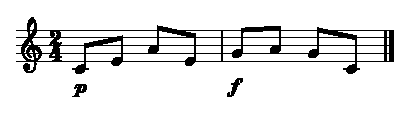
\includegraphics[width=0.7\textwidth]{chapters/cap-musica-basica/matiz1-1.eps}
\caption{Melodia com diferentes matizes.}
\label{fig:matiz1-1}
\end{figure}

Para aumentar ou diminuir gradativamente a intensidade do som,
também podem ser usados sinais ou palavras \cite[pp. 215]{medteoria} \cite[pp. 117]{mascarenhascurso}:
\begin{itemize}
\item Crescendo (cresc.); símbolo: $<$
\item Decrescendo (decresc.) ou diminuindo (dim.); símbolo: $>$
\end{itemize}

\begin{example}[Indicando matizes com letras:]
A Figura \ref{fig:matiz2-1} mostra uma melodia 
que usa em todo o primeiro compasso uma mudança gradual de matiz desde o ``piano'' ate o ``forte'',
e em todo o segundo compasso uma mudança gradual do matiz desde o ``forte'' ate o ``piano''.
\end{example}
\begin{figure}[!h]
\centering
 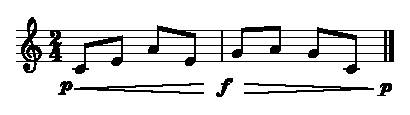
\includegraphics[width=0.7\textwidth]{chapters/cap-musica-basica/matiz2-1.eps}
\caption{Melodia com mudanças graduais de matizes.}
\label{fig:matiz2-1}
\end{figure}


%\PRLsep{Simbolos como sinais de intesidade}


%%%%%%%%%%%%%%%%%%%%%%%%%%%%%%%%%%%%%%%%%%%%%%%%%%%%%%%%%%%%%%%%%%%%%%%%%%%%%%%%
\section{Repetições}
\index{Música!Repetições}
\label{sec:repetitions}

\subsection{Repetições de compassos}
\index{Música!Repetições de compassos}
\label{sec:repetitions:compass}

É possivel expressar a repetição de um o mais compassos usando o simbolo $\%$ 
\cite[pp. 249]{medteoria} \cite[pp. 111]{mascarenhascurso}.
A Figura \ref{fig:repeat-bar1-1} mostra o uso de repetições para escrever de forma compacta uma melodia.
A Figura \ref{fig:repeat-bar2-1} mostra a forma expandida da melodia expressada na Figura \ref{fig:repeat-bar1-1}.
\begin{figure}[!h]
\centering
    \begin{subfigure}[b]{0.6\textwidth}
        \includegraphics[width=0.9\textwidth]{chapters/cap-musica-basica/repeat-bar1-1.eps}
        \caption{Forma compacta.}
        \label{fig:repeat-bar1-1}
    \end{subfigure}
    \begin{subfigure}[b]{0.6\textwidth}
        \includegraphics[width=0.9\textwidth]{chapters/cap-musica-basica/repeat-bar2-1.eps}
        \caption{Forma expandida.}
        \label{fig:repeat-bar2-1}
    \end{subfigure}
\caption{Uso de repetições de compassos.}
\label{fig:repeat-bar1}
\end{figure}


\subsection{Repetições de trechos musicais}
\index{Música!Repetições de trechos}
\label{sec:repetitions:manycompass}

\subsubsection{Ritonelo}
\index{Música!Ritonelo}
É possivel expressar a repetição de um trecho de música usando o ``ritnonelo'' 
que tem um simbolo ``$:|$'' \cite[pp. 237]{medteoria} \cite[pp. 168]{cardoso1973curso}.

\begin{example}[Uso de ritnonelo final:]Se temos uma melodia com compasses $A$, $B$ e $C$,
então estas duas formas são equivalentes:
\begin{itemize}
\item $A~B~C~:|$
\item $A~B~C~A~B~C$
\end{itemize}
\end{example}


\begin{example}[Uso de ritnonelo inicial final:]Se temos uma melodia com compasses $A$, $B$ e $C$,
então estas duas formas são equivalentes:
\begin{itemize}
\item $ A|:B~C:|$
\item $A~B~C~B~C$
\end{itemize}
\end{example}

A Figura \ref{fig:ritonelo1-1} mostra o uso de repetições para escrever de forma compacta uma melodia.
A Figura \ref{fig:ritonelo2-1} mostra a forma expandida da melodia expressada na Figura \ref{fig:ritonelo1-1}.
\begin{figure}[!h]
\centering
    \begin{subfigure}[b]{0.75\textwidth}
        \includegraphics[width=0.9\textwidth]{chapters/cap-musica-basica/ritonelo1-1.eps}
        \caption{Forma compacta.}
        \label{fig:ritonelo1-1}
    \end{subfigure}
    \begin{subfigure}[b]{0.75\textwidth}
        \includegraphics[width=0.9\textwidth]{chapters/cap-musica-basica/ritonelo2-1.eps}
        \caption{Forma expandida.}
        \label{fig:ritonelo2-1}
    \end{subfigure}
\caption{Uso de repetições de trechos de música.}
\label{fig:ritonelo1}
\end{figure}

\subsubsection{Ritonelo com expressoes de 1ra e 2da vez}
Se um trecho de musica deve ser repetido mas com um diferente final cada vez,
então deve ser usado a expressão ``1ra vez'' e ``2da vez''
\cite[pp. 239]{medteoria} \cite[pp. 169]{cardoso1973curso}.

A Figura \ref{fig:ritonelo-times1-1} mostra o uso de repetições para escrever de forma compacta uma melodia.
A Figura \ref{fig:ritonelo-times2-1} mostra a forma expandida da melodia expressada na Figura \ref{fig:ritonelo-times1-1}.
\begin{figure}[!h]
\centering
    \begin{subfigure}[b]{0.75\textwidth}
        \includegraphics[width=0.9\textwidth]{chapters/cap-musica-basica/ritonelo-times1-1.eps}
        \caption{Forma compacta.}
        \label{fig:ritonelo-times1-1}
    \end{subfigure}
    \begin{subfigure}[b]{0.75\textwidth}
        \includegraphics[width=0.9\textwidth]{chapters/cap-musica-basica/ritonelo-times2-1.eps}
        \caption{Forma expandida.}
        \label{fig:ritonelo-times2-1}
    \end{subfigure}
\caption{Uso de repetições de trechos de música com expressoes de vez.}
\label{fig:ritonelo-times1}
\end{figure}


%%%%%%%%%%%%%%%%%%%%%%%%%%%%%%%%%%%%%%%%%%%%%%%%%%%%%%%%%%%%%%%%%%%%%%%%%%%%%%%%




\chapterimage{chapter_head_flauta1.pdf} % Chapter heading image

\chapter{\textcolor{red}{Fundamentos de composição musical}}
Nas seguintes sub seções abordaremos alguns conceitos importantes para iniciar o estudo da dacomposição musical;
porem, não aprofundaremos demasiado em toda a teoria, 
devido a que as explicações mostradas aqui, estão
orientadas para um público interessado na dança, que necesita a principio
ferramentas para entender a musica e melhorar sua percepção musical. 


%%%%%%%%%%%%%%%%%%%%%%%%%%%%%%%%%%%%%%%%%%%%%%%%%%%%%%%%%%%%%%%%%%%%%%%%%%%%%%%%
%%%%%%%%%%%%%%%%%%%%%%%%%%%%%%%%%%%%%%%%%%%%%%%%%%%%%%%%%%%%%%%%%%%%%%%%%%%%%%%%
\section{Articulação}
\label{sub:Articulation}
\index{Música!Articulação}

Nas partituras podemos ver alguns símbolos, 
que o compositor coloca como indicação ao interprete,
para informar como as notas musicais devem ser executadas ou 
articuladas entre sim \cite[pp. 56]{alves2004teoria}.
%%%%%%%%%%%%%%%%%%%%%%%%%%%%%%%%%%%%%%%%%%%%%%%%%%%%%%%%%%%%%%%%%%%%%%%%%%%%%%%%
\subsection{Legato }
\label{subsec:Legato}
\index{Música!Legato}
O  ``legato'' é um símbolo  que indica uma ligadura de expressão entre as notas,
neste caso a informação que da ao compositor é que as
notas devem ser executadas sem interrupções e
criando uma mudança de tons gradual para passar de uma nota musical a outra \cite[pp. 56]{alves2004teoria} \cite[pp. 18]{holland2013music}.

\begin{example}
A Figura \ref{fig:legato1} mostra um exemplo de uso do legato. 
Alguns instrumentos podem facilmente articular um legato, por exemplo o violino.
\end{example}

\begin{figure}[h!]
\centering
\begin{abc}[name=abc-legato1,width=0.80\linewidth]
X: 1 % start of header
K: C % scale: C major
M: 2/4 %meter - compasso
 (G2 E2 | G1  A1  G1 E1 )|
\end{abc}
\caption{Melodia com notas que devem ser executadas de forma ligada.}
\label{fig:legato1}
\end{figure}

%%%%%%%%%%%%%%%%%%%%%%%%%%%%%%%%%%%%%%%%%%%%%%%%%%%%%%%%%%%%%%%%%%%%%%%%%%%%%%%%
\subsection{Staccato}
\label{subsec:Staccato}
\index{Música!Staccato}

O staccato é um símbolo, desenhado com um ponto (.), 
que indica a diminuição na \hyperref[sec:pos:Duracion]{\textbf{duração}} de uma nota (aproximadamente um 50\%), 
dando nela um efeito de separação ou destaque \cite[pp. 56]{alves2004teoria} \cite[pp. 16]{holland2013music}.

\begin{example}
A Figura \ref{fig:staccato1a} mostra um exemplo de uso do staccato. 
Na Figura \ref{fig:staccato1b} podemos ver uma escrita equivalente, sem o uso do símbolo de staccato.
\end{example}

\begin{figure}[h!]
\centering
\begin{subfigure}[c]{0.80\textwidth}
\begin{abc}[name=abc-staccato1a]
X: 1 % start of header
K: C % scale: C major
M: 2/4 %meter - compasso
 .G2 .E2 | .G1  .A1  .G1 .E1 | 
\end{abc}
\caption{Notação de notas musicais em staccato.}
\label{fig:staccato1a}
\end{subfigure}
~ %
\begin{subfigure}[c]{1.00\textwidth}
\begin{abc}[name=abc-staccato1b]
X: 1 % start of header
K: C % scale: C major
M: 2/4 %meter - compasso
 G1 z1 E1 z1 | G1/2 z1/2 A1/2 z1/2 G1/2 z1/2 E1/2 z1/2 | 
\end{abc}
\caption{Forma de execução de notas musicais em staccato.}
\label{fig:staccato1b}
\end{subfigure}
\caption{Melodia com notas que devem ser executadas em staccato.}
\label{fig:staccato1}
\end{figure}

\subsubsection{Staccatissimo}

O staccatissimo, staccato seco ou martelado é um símbolo, com uma função similar ao staccato;
porém indica uma diminuição maior na \hyperref[sec:pos:Duracion]{\textbf{duração}} 
de nota (aproximadamente ao 25\%) \cite[pp. 56]{alves2004teoria} \cite[pp. 16]{holland2013music}.

\begin{example}
A Figura \ref{fig:staccatissimo1a} mostra um exemplo de uso do staccatissimo. 
Na Figura \ref{fig:staccatissimo1b} podemos ver uma escrita equivalente, sem o uso do símbolo de staccatissimo.
\end{example}

\begin{figure}[h!]
\centering
\begin{subfigure}[c]{0.80\textwidth}
\begin{abc}[name=abc-staccatissimo1a]
X: 1 % start of header
K: C % scale: C major
M: 2/4 %meter - compasso
 !wedge!G2 !wedge!E2 | !wedge!G1  !wedge!A1  !wedge!G1 !wedge!E1 | 
\end{abc}
\caption{Notação de notas musicais em staccatissimo.}
\label{fig:staccatissimo1a}
\end{subfigure}
~ %
\begin{subfigure}[c]{1.00\textwidth}
\begin{abc}[name=abc-staccatissimo1b]
X: 1 % start of header
K: C % scale: C major
M: 2/4 %meter - compasso
 G1/2 z3/2 E1/2 z3/2 | G1/4 z3/4 A1/4 z3/4 G1/4 z3/4 E1/4 z3/4 | 
\end{abc}
\caption{Forma de execução de notas musicais em staccatissimo.}
\label{fig:staccatissimo1b}
\end{subfigure}
\caption{Melodia com notas que devem ser executadas em staccato.}
\label{fig:staccatissimo1}
\end{figure}

%%%%%%%%%%%%%%%%%%%%%%%%%%%%%%%%%%%%%%%%%%%%%%%%%%%%%%%%%%%%%%%%%%%%%%%%%%%%%%%%
\subsection{Tenuto}
\label{subsec:Tenuto}
\index{Música!Tenuto}

O tenuto (ou sostenuto) é um símbolo desenhado com uma linha reta (-)  
que indica que deve ser sustentada a 
\hyperref[sec:pos:Duracion]{\textbf{duração}} e a 
\hyperref[sec:pos:Intensidade]{\textbf{intensidade}} da nota ao máximo \cite[pp. 56]{alves2004teoria} \cite[pp. 17]{holland2013music}.

\begin{example}
A Figura \ref{fig:tenuto1} mostra um exemplo de uso do tenuto. 
\end{example}


\begin{figure}[h!]
\centering
\begin{abc}[name=abc-tenuto1,width=0.80\linewidth]
X: 1 % start of header
K: C % scale: C major
M: 2/4 %meter - compasso
 !tenuto!G2 !tenuto!E2 | !tenuto!G1  !tenuto!A1  !tenuto!G1 !tenuto!E1 |
\end{abc}
\caption{Melodia com notas que devem ser executadas de forma sustenido.}
\label{fig:tenuto1}
\end{figure}

%%%%%%%%%%%%%%%%%%%%%%%%%%%%%%%%%%%%%%%%%%%%%%%%%%%%%%%%%%%%%%%%%%%%%%%%%%%%%%%%
\subsection{Accénto}
\label{subsec:Accento}
\index{Música!Accénto}

O accénto é um símbolo desenhado com (>) 
que indica que a nota deve ser enfatizada; 
ou seja que a nota deve receber um aumento de \hyperref[sec:pos:Intensidade]{\textbf{intensidade}} \cite[pp. 56]{alves2004teoria}.

\begin{example}
A Figura \ref{fig:accento1} mostra um exemplo de uso do accénto.
Nela os tempos fracos tem um aumento de intensidade provocando \hyperref[sec:contratempo]{\textbf{contratempos}}. 
\end{example}


\begin{figure}[h!]
\centering
\begin{abc}[name=abc-accento1,width=0.80\linewidth]
X: 1 % start of header
K: C % scale: C major
M: 2/4 %meter - compasso
 G2 !>!E2 | G1  !>!A1  !>!G1 !>!E1 |
\end{abc}
\caption{Melodia com notas que devem ser executadas de forma sostenida.}
\label{fig:accento1}
\end{figure}
 


%%%%%%%%%%%%%%%%%%%%%%%%%%%%%%%%%%%%%%%%%%%%%%%%%%%%%%%%%%%%%%%%%%%%%%%%%%%%%%%%
\section{\textcolor{red}{Motivos}}
\index{Música!Motivos}
\index{Música!Motif}

%%%%%%%%%%%%%%%%%%%%%%%%%%%%%%%%%%%%%%%%%%%%%%%%%%%%%%%%%%%%%%%%%%%%%%%%%%%%%%%%
\section{\textcolor{red}{Frase}}\index{Música!Frase}
\cite[pp. 150]{medteoria}


A frase melódica
% https://pt.wikipedia.org/wiki/Frase_(música)
Frase rítmica
% rhythmic phrase
% https://books.google.com.br/books?id=KjSJcjIBvjcC&pg=PA5&dq=rhythmic+phrase&hl=es-419&sa=X&ved=0ahUKEwiqj6r-utrhAhV4E7kGHaO2AXAQ6AEIKTAA#v=onepage&q=rhythmic%20phrase&f=false
% https://en.wikipedia.org/wiki/Phrase_(music)
%%%%%%%%%%%%%%%%%%%%%%%%%%%%%%%%%%%%%%%%%%%%%%%%%%%%%%%%%%%%%%%%%%%%%%%%%%%%%%%%
\section{\textcolor{red}{Período}}\index{Música!Período}
% https://en.wikipedia.org/wiki/Period_(music)
%%%%%%%%%%%%%%%%%%%%%%%%%%%%%%%%%%%%%%%%%%%%%%%%%%%%%%%%%%%%%%%%%%%%%%%%%%%%%%%%
\section{\textcolor{red}{Sentencia}}\index{Música!Sentencia}
% https://en.wikipedia.org/wiki/Sentence_(music)
%%%%%%%%%%%%%%%%%%%%%%%%%%%%%%%%%%%%%%%%%%%%%%%%%%%%%%%%%%%%%%%%%%%%%%%%%%%%%%%%
\section{\textcolor{red}{Riff}}\index{Música!Riff}
% https://es.wikipedia.org/wiki/Riff

%%%%%%%%%%%%%%%%%%%%%%%%%%%%%%%%%%%%%%%%%%%%%%%%%%%%%%%%%%%%%%%%%%%%%%%%%%%%%%%%
\section{\textcolor{red}{Fraseio}}
\index{Música!Fraseio}

% https://es.wikipedia.org/wiki/Fraseo
% https://en.wikipedia.org/wiki/Musical_phrasing

%%%%%%%%%%%%%%%%%%%%%%%%%%%%%%%%%%%%%%%%%%%%%%%%%%%%%%%%%%%%%%%%%%%%%%%%%%%%%%%%
\section{\textcolor{red}{Cadencia}}
\index{Música!Cadencia}

\cite[pp. 111]{holst1998abc}

% https://es.wikipedia.org/wiki/Cadencia_(música)

% https://en.wikipedia.org/wiki/Cadence

cadencia harmonica \cite[pp. 67]{melcior1859diccionario} \cite[pp. 60]{pedrell2009diccionario}

cadencia melodica \cite[pp. 66]{melcior1859diccionario} \cite[pp. 60]{pedrell2009diccionario}




\chapterimage{chapter_head_palco1.pdf} % Chapter heading image

\chapter{\textcolor{red}{Tópicos de composição musical}}


%%%%%%%%%%%%%%%%%%%%%%%%%%%%%%%%%%%%%%%%%%%%%%%%%%%%%%%%%%%%%%%%%%%%%%%%%%%%%%%%
\section{\textcolor{red}{Agrega letra à música}}

\cite[pp. 149]{medteoria}
% https://es.wikipedia.org/wiki/Letra_(m%C3%BAsica)
% https://vox-technologies.com/blog/como-escribir-letras-de-canciones


%%%%%%%%%%%%%%%%%%%%%%%%%%%%%%%%%%%%%%%%%%%%%%%%%%%%%%%%%%%%%%%%%%%%%%%%%%%%%%%%
\section{\textcolor{red}{Partes de uma música}}
% https://en.wikipedia.org/wiki/Section_(music)

%%%%%%%%%%%%%%%%%%%%%%%%%%%%%%%%%%%%%%%%%%%%%%%%%%%%%%%%%%%%%%%%%%%%%%%%%%%%%%%%
\section{\textcolor{red}{Componer musica por capas}}
% https://www.escribircanciones.com.ar/icomo-componer-musica/190-metodo-de-composicion-por-capas.html




%----------------------------------------------------------------------------------------
%----------------------------------------------------------------------------------------
%----------------------------------------------------------------------------------------
%	PART
%----------------------------------------------------------------------------------------
\part{Memoria, aprendizagem e dança}
%----------------------------------------------------------------------------------------
%	CHAPTER 2
%----------------------------------------------------------------------------------------
\chapterimage{chapter_head_math.pdf} % Chapter heading image

\chapter{Estágios do ciclo da aprendizagem}
\label{cap:aprendizagem}




\section{Estágios da aprendizagem}
\label{sec:aprendizagem}

Quando desejamos apreender uma nova habilidade ou conhecimento, já seja tocar o piano,
resolver problemas matemáticos,
jogar futebol, ou dançar; devemos atravessar por um processo de aprendizagem dividido em estágios;
o conhecimento destes estágios nos permitirá modelar melhores estrategias e exercícios para o aprendizado,
focando-nos no estagio em que se encontre cada pessoa.

De acordo com a programação neuro linguística (PNL), 
entre os estágios do processo (ciclo) de aprendizagem podemos achar:
a incompetência inconsciente, a incompetência consciente, 
a competência consciente e finalmente a competência inconsciente 
\cite[pp. 249]{seymourtreinando} \cite[pp. 10]{passadori7} \cite{de2013treinamentos};
ver Tabela \ref{tab:learning1}.

\begin{table}[!h]
  \centering
  \begin{tabular}{|l||l|l|}
   \hline
    ~             & incompetência & competência \\ \hline \hline
    inconsciente  & Estágio 1     & Estágio 4   \\ \hline
    consciente    & Estágio 2     & Estágio 3   \\ \hline
  \end{tabular}
  \caption{Estágios da aprendizagem.}
  \label{tab:learning1}
\end{table}

\begin{description}
%%%%%
\item[incompetência inconsciente:] Neste estágio da aprendizagem não temos consciência do que devemos fazer ou aprender,
e consequentemente temos incompetência na área que desejamos desenvolve-nos e/ou vivemos numa ``alegre ignorância'';
``você não sabe o que não sabe'' \cite[pp. 29, 252]{seymourtreinando} \cite{carnegie2014lideranca} \cite{de2013treinamentos}.
Existe a possibilidade que ao desconhecer nossas próprias limitações,
tendamos achar que o problema da falta de sucesso é externo a nós \cite[pp. 10]{passadori7}.
%%%%%
\item[incompetência consciente:] Neste estágio você sabe o que deve fazer ou aprender,
\label{ref:IncompetenciaConsciente}
porem não consegue realizar a tarefa de forma competente;
por este motivo a tarefa exige toda nossa atenção, 
este estágio da aprendizagem pode trazer algum desconforto,
mas a taxa de aprendizagem é maior neste estágio;
``você descobre o que não sabe, consequentemente, descobre uma incompetência nesse ponto''
\cite[pp. 29]{seymourtreinando} \cite{carnegie2014lideranca} \cite[pp. 10, 11]{passadori7} \cite{de2013treinamentos}.
%%%%%
\item[competência consciente:] 
\label{ref:CompetenciaConsciente}
Neste estagio somos competentes, 
porem precisamos de toda nossa atenção consciente 
para realizar uma determinada tarefa; a tarefa ainda não tem-se tornado um hábito em nós 
\cite[pp. 30, 249]{seymourtreinando} \cite{carnegie2014lideranca} \cite{de2013treinamentos}.
Esta é a fase do condicionamento positivo,
onde a pessoa deve estar em exercício continuo com reforços positivos para fixar o aprendizado \cite[pp. 11]{passadori7}.
%%%%%
\item[competência inconsciente:] 
\label{ref:CompetenciaInconsciente}
Neste estágio a habilidade em estudo tem sido plenamente integrada em nós, 
e podemos realizá-la sem esforço, de forma inconsciente, com confiança e naturalidade, 
de modo que podemos realizar outras atividades em paralelo;
``maestria intuitiva e instintiva'' \cite[pp. 30, 249]{seymourtreinando} \cite[pp. 11]{passadori7} \cite{de2013treinamentos}.
\end{description}


\begin{elaboracion}[title=O cerebelo e o comportamento inconsciente, width= 1.00\linewidth]
%   https://books.google.com.br/books?id=cf3AAdIH1UQC&pg=PA35&dq=compet%C3%AAncia+inconsciente+cerebelo&hl=pt-BR&sa=X&ved=0ahUKEwir6qfn4OzkAhVzKLkGHTvZD1wQ6AEIUzAF#v=onepage&q=compet%C3%AAncia%20inconsciente%20cerebelo&f=false
O cerebelo (``cérebro pequeno'' em latim) é uma protuberância ampla e convoluta,
localizada na fossa posterior do crânio, 
e está conectada à parte traseira do tronco encefálico \cite[pp. 93]{gazzanigaciencia} \cite[pp. 87]{carneiro2004atlas}
\cite[pp. 516]{bearneurociencias}.

A função mais evidente do cerebelo é a aprendizagem motora e a memoria motora,
sendo o grande coordenador da ação muscular ``inconsciente'';
ao contrario do cérebro que atua de forma ``consciente'' 
\cite[pp. 93]{gazzanigaciencia} \cite[pp. 87]{carneiro2004atlas} \cite[pp. 516]{bearneurociencias}.

O cerebelo é quem nos permite estar caminhado de forma inconsciente,
e ao mesmo tempo poder raciocinar uma fala com alguém ou planejar nosso dia de trabalho.
\end{elaboracion}



\section{Ciclo da aprendizagem - PDCA}
\label{sec:cicloaprendizagem}
O ciclo que seguimos para potencializar nossa aprendizagem \cite[pp. 13]{mumford2001aprendendo},
em muitos aspectos se parece ao ciclo, para a melhoria continua, na gerencia de projetos 
\cite[pp. 4]{caloba2018gerenciamento} \cite[pp. 59]{teixeira2018gestao}.
Na literatura, este é conhecido como ``ciclo PDCA'';
a sigla vem das palavras em inglês: ``Plan'', ``Do'', ``Check'' e ``Act'';
estas podem ser interpretadas como: Planejar, fazer, verificar e atuar em consequência
\cite[pp. 59]{teixeira2018gestao} \cite[pp. 4]{caloba2018gerenciamento}.
Este fluxo de trabalho, também é chamado ``ciclo de Shewhart'' em honor a seu inventor,
ou ``ciclo de Demming'' em honor a um de seus grandes difusores no Japão
\cite[pp. 59]{teixeira2018gestao} \cite[pp. 4]{caloba2018gerenciamento}.

A Figura \ref{fig:ciclopdca} mostra em detalhe o fluxo de trabalho no ciclo PDCA.
\begin{figure}[!h]
  \centering
    \includegraphics[width=0.55\textwidth]{chapters/cap-learning/ciclo2.eps}
\caption{Ciclo PDCA.}
\label{fig:ciclopdca}
\end{figure}

\begin{description}
\item[Planejar:] Estabelecemos nosso objetivo no aprendizado; 
realizamos um planejamento do caminho que seguiremos para atingir nossos objetivos.
\item[Fazer, desenvolver:] Pomos em prática o trabalho anteriormente planejado;
coletamos dados sobre nosso desenvolvimento nas tarefas escolhidas.
\item[Verificar, conferir:] Comparamos o resultado obtido com o esperado;
realizamos uma avaliação de nosso despenho e competência.
\item[Atuar, agir, ajustar:] Tomamos ações corretivas no nosso plano de trabalho,
para diminuir as diferenças entre o resultado obtido e o esperado.
\end{description}


\begin{tcbattention}
Uma pessoa inteligente aprende do seus próprios erros,
uma pessoa sabia aprende dos erros dos demais.
\begin{flushright}
Fernando P. R.
\end{flushright}
\end{tcbattention}


\section{Percepção e aprendizagem}
\label{sec:percepcionaprendizagem}

O ser humano entende o mundo que lhe rodeia mediante o uso do seus sentidos,
de modo que suas percepções podem ser de caráter \cite[pp. 28]{ready2010pnl}:
\begin{itemize}
\item visual (olhos), 
\item auditivo (ouvidos),
\item cinestésico (emoções e tato), 
\item olfativo (nariz) e
\item gustativo (gusto).
\end{itemize}
Entre todas estas possíveis fontes de informação,
pelo geral, quando estamos em nosso momento de maior estresse,
cada um de nós manifestamos preferencia por alguma destas 5 fontes de informação;
este sentido preferenciado é conhecido como ``sistema figurativo'' ou ``representação primordial''
\cite[pp. 28]{ready2010pnl}.

Seja metafórica ou real nossa fonte de conflito, o estresse sempre estará presente,
e nosso corpo acude a nossa representação primordial para obter informação.
Quando tentamos alcançar a competência numa área desfavorável para nós\footnote{Estágio 
2 de nosso aprendizado visto na Pag. \pageref{ref:IncompetenciaConsciente}.},
podemos atingir o estresse, consequentemente nosso corpo acudirá com atenção a 
nossa representação primordial;
pelo que é interessante fazer um exame de autoconhecimento, 
para poder saber qual é este sentido em nós e assim otimizar nosso processo de aprendizagem.


% https://books.google.com.br/books?id=zxYIsvdXo_QC&pg=PA137&dq=modo+de+aprender+cinest%C3%A9sico&hl=pt-BR&sa=X&ved=0ahUKEwi1lJGkye7kAhWvH7kGHb2TCOoQ6AEILzAB#v=onepage&q=cinest%C3%A9sico&f=false
% https://books.google.com.br/books?id=ioi2Ic-FRWUC&pg=PA152&dq=visual+auditivo+cinest%C3%A9sico&hl=pt-BR&sa=X&ved=0ahUKEwjwou29ye7kAhU-IbkGHVpBAI0Q6AEIOTAD#v=onepage&q=visual%20auditivo%20cinest%C3%A9sico&f=false


\begin{elaboracion}[title=Ditado chines, width= 1.00\linewidth]
Existe um velho ditado chines atribuído a Confúcio \cite[pp. 60, 63]{AprendendoInteligencia2008} \cite[pp. 9]{abe2002introducao}:\\
\begin{center}
    \includegraphics[width=0.8\textwidth]{chapters/cap-learning/ditadochines.eps}
\end{center}
\end{elaboracion}

\chapterimage{chapter_head_2.pdf} % Chapter heading image

\chapter{Caraterísticas da dança}

\begin{tcbinformation} 
\textbf{Dança:}
\index{Dança}
\label{def:DancaGeral}
Mas que uma simples palavra, a dança é um conceito; e como tal, esta representa 
uma ideia, juízo ou opinião; pelo que podemos ter múltiplas pontos de vista do que é a dança \cite[pp. 2]{Rejane2011}.
%Assim podemos listar os seguintes significados a palavra dança:
\begin{itemize}
\item ``Sequência de movimentos corporais executados de maneira ritmada, 
em geral ao som de música'' \cite[pp. 604]{ferreira1999novo}.
\item ``A arte de mover o corpo segundo a relação estabelecida entre tempo e espaço,
gerada pelo ritmo e a composição coreográfica'' \cite[pp. 17]{bencardinidanca}
\item A dança é a movimentação corporal, que tem como proposito, 
a expressão emocional, sentimental, lúdica ou artística.
%% correr para chegar ao otro lado exersicio, correr paa expresarse dança.
\end{itemize}
\end{tcbinformation} 

\begin{center}
\begin{tabular}{lll}
~ & Sim & Não \\
A dança é sempre feita com música? & \NoCheckedItem & \CheckedItem \\ %\hline
É necessário um par para dançar? & \NoCheckedItem & \CheckedItem \\ %\hline
A dança é uma arte? & \CheckedItem & \NoCheckedItem \\ %\hline
A dança tem necessariamente um significado? & \NoCheckedItem & \CheckedItem \\ %\hline
\end{tabular}
\end{center}
%%%%%%%%%%%%%%%%%%%%%%%%%%%%%%%%%%%%%%%%%%%%%%%%%%%%%%%%%%%%%%%%%%%%%%%%%%%%%%%%
%%%%%%%%%%%%%%%%%%%%%%%%%%%%%%%%%%%%%%%%%%%%%%%%%%%%%%%%%%%%%%%%%%%%%%%%%%%%%%%%
\section{Elementos da dança}
\index{Elementos da dança}
\index{Rudolf Laban}
\begin{wrapfigure}{l}{0.22\textwidth}
\centering
\includegraphics[width=0.20\textwidth]{chapters/cap-dance-elements/Labanotation2.eps}
\caption{Símbolos de Labanotation.}
\label{fig:elementosdanca1}
\end{wrapfigure}
 No seu estudo da teoria do movimento, Rudolf Laban (1879-1958) fez significativas contribuições e
observações na área da ``dança  educacional'',  
realizando contribuições como, a criação de uma forma escrita de notação coreográfica (Labanotation), 
e um  analises preciso do movimento na dança, entre outros \cite[pp. 18]{elementosdanca2017} \cite[pp. 11]{paine2014complete}.
Com seu estudo do movimento, 
Laban  deu sustento ao ensino da dança educacional moderna e 
presentou 16 temas ou áreas-chave no analises do movimento, 
sendo estes ligados a estágios no desenvolvimento da criança em desenvolvimento \cite[pp. 12]{paine2014complete}.

Nas décadas dos anos 1960 e 1970, 
viu-se  na Grã-Bretanha um crescimento importante na dança contemporânea;
a popularidade deste estilo foi devido a que este era menos exclusivo que o balé, 
com técnicas baseadas em movimentos mais naturais, 
além de ter a vantagem de ser unissex e pouco pretensioso.
Assim, estabelecimentos como a ``London School of Contemporary Dance'',
ou bailarinos treinados trabalhando de forma independente,
ofereciam oficinas para faculdades e escolas,
dando um ``enfoque profissional à dança'' \cite[pp. 12]{paine2014complete}.

\begin{wrapfigure}{r}{0.45\textwidth}
\centering
\smartdiagram[bubble diagram]{Dança, Corpo, Tempo, Espaço, Relações, Dinâmicas}
%%\includegraphics[width=0.42\textwidth]{chapters/cap-dance-elements/DanceElements.eps}
\caption{Elementos da dança}
\label{fig:elementosdanca1}
\end{wrapfigure}
Por outro lado, em 1994, Jacqueline Smith-Autard, uma das principais educadoras britânicas de dança, 
propôs um modelo intermediário (``midway model''), entre o educacional e o profissional, 
usando as áreas mais interessantes propostas por Laban \cite[pp. 12]{paine2014complete}.

Seguindo esses modelos, é comum achar na literatura atual 
\cite[pp. 4]{carline2011lesson}       %% corpo, espaço, esforço , relacionamentos
\cite[pp. 13,27]{paine2014complete}   %% corpo, espaço, esforço , relacionamentos
\cite[pp. 69]{schrader2005sense}      %% tempo, espaço, esforço
\cite[pp. 131]{mccutchen2006teaching},%% tempo, corpo, espaço, esforço , relacionamentos
 análises  da dança dividindo esta entre três a cinco elementos,
dependendo da visão do autor.
Estes elementos da dança são: O corpo, as dinâmicas, o espaço, os relacionamentos, e o tempo;
a Figura \ref{fig:elementosdanca1} mostra uma representação gráfica destes elementos.



%%%%%%%%%%%%%%%%%%%%%%%%%%%%%%%%%%%%%%%%%%%%%%%%%%%%%%%%%%%%%%%%%%%%%%%%%%%%%%%%
\subsection{Corpo}
\caracterelement{Do corpo ou das ações}{O que o corpo está fazendo?}
Na dança existem muitos motivos para realizar uma ação corporal;
cada um destes motivos procura ter um significado, seja este prático ou estético, literal ou metafórico \cite[pp. 5]{carline2011lesson}.
As ações realizadas pelo corpo são moldadas pelas relações com os outros elementos da dança,
como as dinâmicas, o uso do espaço, o tempo, e as relações com os outros \cite[pp. 5]{carline2011lesson}.
Algumas das ações mais básicas que podemos realizar com o corpo são,
desloca-nos, pular, virar-nos, gesticular, ou quietude \cite[pp. 27]{paine2014complete}.

\textbf{Deslocamentos:} Implica a transferência do peso do corpo 
para variar de posição no espaço usando na dança;
existem várias formas de realizar esta ação,
por exemplo podemos faze-o pisando, deslizando, rastejando \cite[pp. 28]{paine2014complete}.

\textbf{Pular:} (ou elevar-nos) descreve a ações que provocam que o corpo saia e volta ao chão,
impulsando-nos pelo uso das pernas; as distancias alcançadas podem ser pequenas ou longas,
dependendo do método que usemos no movimento  \cite[pp. 28]{paine2014complete}. 

\textbf{Virar:} envolve movimentos de rotação em torno de um eixo.
Este giro não tem que ser necessariamente completo ($360^o$),
e podem ser trabalhados níveis, como giros de um ângulo especifico;
os movimentos de giro podem ser iniciados por alguma parte do corpo, 
não necessariamente pelos pés \cite[pp. 29]{paine2014complete}.

\textbf{Gesto:} Implica o movimento de uma ou varias partes do corpo,
que não envolve suporte ou transferência de peso
(ex: movimentos axiais, como flexão, alongamento e torção);
os gestos enriquecem o conteúdo expressivo de uma dança,
onde são usados para contar uma história, 
usando um vocabulário simbólico reconhecido popular ou tradicionalmente 
\cite[pp. 29]{paine2014complete}.

\textbf{Quietude:} descreve a capacidade de interromper nosso movimento, 
controlando no processo nosso equilíbrio \cite[pp. 29]{paine2014complete}.


A consciência corporal se centra no estudo do uso controlado do corpo, 
à medida que as movimentações são exploradas,
já sejam  estes movimentos realizados pelo corpo inteiro,
ou por partes isoladas deste \cite[pp. 5]{carline2011lesson}.
O tema da consciência corporal será abordado com maior aplitude  na Seção \ref{sec:BodyAwareness}.


%%%%%%%%%%%%%%%%%%%%%%%%%%%%%%%%%%%%%%%%%%%%%%%%%%%%%%%%%%%%%%%%%%%%%%%%%%%%%%%%
\subsection{Dinâmica (esforço)}
\caracterelement{Das dinâmicas}{Como o corpo está se movendo?}
As dinâmicas no movimento 
indicam o jeito em que a energia será usada e direcionada no corpo durante a dança \cite[pp. 131, 136]{mccutchen2006teaching};
além de provocar em nossos movimentos algo que poderia ser definido, metaforicamente, como textura ou cor;
dando uma identidade própria a cada movimento, dependendo da dinâmica utilizada;
Por exemplo, não é o mesmo dar um passo de forma lenta como tentando não fazer barulho,
que dar o passo caindo como se estivéssemos bêbados.

Rudolf Laban, no seu estudo do movimento, 
dividiu as dinâmicas (ou ``esforço'' na notação de Laban) 
em quatro categorias ou fatores: peso, tempo, espaço e fluxo 
\cite[pp. 5]{carline2011lesson}
\cite[pp. 30]{paine2014complete}.
Porem, o modelo de Laban não é a única forma em que podemos fatorar as dinâmicas,
de modo que, inclusive a escolha do modelo para descrever as dinâmicas,
influencia na textura percebina na realização do movimento \cite[pp. 30]{paine2014complete}. 

Uma explicação detalhada, dos fatores em que podemos dividir as 
\hyperref[subsec:fatordinamica]{\textbf{dinâmicas do movimento}},
é descrita na Seção \ref{subsec:fatordinamica}.

%%%%%%%%%%%%%%%%%%%%%%%%%%%%%%%%%%%%%%%%%%%%%%%%%%%%%%%%%%%%%%%%%%%%%%%%%%%%%%%%
\subsection{Espaço} 
\caracterelement{Do espaço}{Para onde o corpo se está movendo?}
A maneira como o espaço é usado pode ajudar a dar interesse visual a nossa dança,
ajudando-nos a contar uma historia como nosso corpo, com um relato que progride no tempo 
\cite[pp. 6]{carline2011lesson}
\cite[pp. 31]{paine2014complete}
\cite[pp. 131, 136]{mccutchen2006teaching}; 
alguns aspectos do espaço que podem ser interessantes de ser explorados na nossa dança são:

\textbf{Espaço pessoal e geral:}  Trabalhamos no nosso espaço pessoal 
quando realizamos movimentos sem deslocamento 
(ex: tremer, subir, girar, pausar ou afundar);
e em nosso espaço geral quando nos deslocamos a outras posições
(ex: caminhar, correr, pular) \cite[pp. 7]{carline2011lesson}
\cite[pp. 32]{paine2014complete}.

\textbf{Caminhos:} Podemos definir o caminho como o padrão desenhado no chão ou no ar, 
quando nos deslocamos,
esta padrão pode ser uma única linha reta ou 
varias conectadas formando padrões mais complexos, 
 com zigue-zagues; também poderíamos ter caminhos curvos e sinuosos; 
inclusive o caminho pode ser uma curva sem inicio né fim como um círculo 
\cite[pp. 7]{carline2011lesson}
\cite[pp. 32]{paine2014complete}.



\textbf{Direções:} Quando trabalhamos com direções, 
temos a possibilidade que nosso movimento seja 
para frente, para trás, para os lados, para cima, para baixo, em diagonal,
entre outras 
\cite[pp. 7]{carline2011lesson}
\cite[pp. 32]{paine2014complete}
\cite[pp. 97-98]{schrader2005sense}. 


\textbf{Formas do corpo:} Com nosso corpo, ou grupo de corpos, podemos criar formas diferentes,
como emular uma parede, uma esfera, 
ou podemos fazer posturas mediante torções, 
e movimentando de forma independente distintas partes do corpo 
\cite[pp. 8]{carline2011lesson}
\cite[pp. 32]{paine2014complete}
\cite[pp. 97]{schrader2005sense}.

\textbf{Níveis:} Quando usamos nosso corpo, 
podemos quantificar nossos movimentos em vários níveis,
relacionados com a distancia com o chão;
por exemplo ao pular, este movimento pode ser baixo, meio ou alto 
\cite[pp. 8]{carline2011lesson}
\cite[pp. 32]{paine2014complete}
\cite[pp. 96]{schrader2005sense}.

\textbf{Posição e proximidade:}  (Preposições espaciais)
É possível usar preposições que nos ajudem a descrever, o uso do espaço,
em relação à posição e proximidade; entre os termos que podemos usar temos:
atrás, na frente, 
acima, abaixo, 
perto, longe, 
através, ao redor
\cite[pp. 32]{paine2014complete} 
\cite[pp. 9]{carline2011lesson}, etc.

\textbf{Dimensão} (Tamanho do movimento ou forma) 
Indica a dimensão de grandeza ou amplitude que terá o movimento ou a forma que executemos;
assim, podemos escolher valores de dimensão entre pequeno e grande 
\cite[pp. 32]{paine2014complete} 
\cite[pp. 99]{schrader2005sense}.

%\textbf{Bases do corpo:}  \cite[pp. 8]{carline2011lesson}.

%\textbf{Extensões para o espaço:}  \cite[pp. 9]{carline2011lesson}.

%%%%%%%%%%%%%%%%%%%%%%%%%%%%%%%%%%%%%%%%%%%%%%%%%%%%%%%%%%%%%%%%%%%%%%%%%%%%%%%%
\subsection{Relacionamento} 
\caracterelement{Das relações}{Com quem ou com que o corpo está se movendo?}
Na dança podemos nos movimentar relacionando-nos com outra pessoa, como na dança social a  dois,
ou em grupos, como em algumas danças folclóricas.
Quando dançamos podemos liderar a dança ou ser seguidores, 
também podemos nos deslocar indo ao encontro com o grupo, 
ou nos separar, dividir, espelhar, contrastar, 
estar em cânone, em uníssono, ou alguma outra forma;
a forma de nos relacionar com os demais são variadas,
inclusive podemos interagir como objetos, sejam estes reais ou imaginários
 \cite[pp. 9]{carline2011lesson}
 \cite[pp. 27, 32-33]{paine2014complete}
\cite[pp. 131, 132, 134]{mccutchen2006teaching}.


%%%%%%%%%%%%%%%%%%%%%%%%%%%%%%%%%%%%%%%%%%%%%%%%%%%%%%%%%%%%%%%%%%%%%%%%%%%%%%%%
\subsection{Tempo}
\caracterelement{Do tempo nas ações}{Quando o corpo realiza uma ação?}
O movimento e as pausas que realizamos estão sempre ligados à variável tempo,
tendo estes um tempo inicial e uma duração;
assim, nossos movimentos, vistos de forma sequencial no tempo, 
seguem um ritmo que pode ser marcado livremente por nós,
ou pode tentar seguir uma fonte externa de informação, como a música;
em qualquer caso é o dançarino o encarregado desta escolha criativa;
existem alguns termos que devem ser parte do vocabulário de dança,
quando estudamos o aproveitamento do elemento tempo,
estes são: 
\hyperref[ref:Pulso]{\textbf{pulso}}, 
\hyperref[sec:Tempo]{\textbf{tempo}}, 
\hyperref[sec:Andamento]{\textbf{andamento}}, 
\hyperref[sec:pos:Ritmo]{\textbf{ritmo}}, e 
\hyperref[def:Metrica]{\textbf{métrica}}
\cite[pp. 82]{schrader2005sense}
\cite[pp. 131, 134, 136]{mccutchen2006teaching}.

%%%%%%%%%%%%%%%%%%%%%%%%%%%%%%%%%%%%%%%%%%%%%%%%%%%%%%%%%%%%%%%%%%%%%%%%%%%%%%%
% FALTA INCLUIR ENERGIA
%%%%%%%%%%%%%%%%%%%%%%%%%%%%%%%%%%%%%%%%%%%%%%%%%%%%%%%%%%%%%%%%%%%%%%%%%%%%%%%
%% https://books.google.com.br/books?id=C0yjXGJ3EEoC&pg=PA131&dq=dynamics+dance+energy&hl=pt-BR&sa=X&ved=0ahUKEwjc472wjrXlAhUeEbkGHbstBbUQ6AEIKTAA#v=onepage&q=dynamics%20%20energy&f=false
%% https://books.google.com.br/books?id=omYS0_FkOWIC&pg=PT169&dq=dynamics+dance+energy&hl=pt-BR&sa=X&ved=0ahUKEwjc472wjrXlAhUeEbkGHbstBbUQ6AEIMjAB#v=onepage&q=dynamics%20energy&f=false
%% https://books.google.com.br/books?id=Z0hoAwAAQBAJ&printsec=frontcover&dq=discovering+dance&hl=pt-BR&sa=X&ved=0ahUKEwif04WJwbXlAhUkILkGHdxnAjEQ6AEIKTAA#v=onepage&q=discovering%20dance&f=false
%%%%%%%%%%%%%%%%%%%%%%%%%%%%%%%%%%%%%%%%%%%%%%%%%%%%%%%%%%%%%%%%%%%%%%%%%%%%%%%
%%%%%%%%%%%%%%%%%%%%%%%%%%%%%%%%%%%%%%%%%%%%%%%%%%%%%%%%%%%%%%%%%%%%%%%%%%%%%%%

%----------------------------------------------------------------------------------------
%----------------------------------------------------------------------------------------
%----------------------------------------------------------------------------------------
%	PART
%----------------------------------------------------------------------------------------
\part{Musicalidade}
\chapterimage{chapter_head_2.pdf} % Chapter heading image

\chapter{Percepção musical}
\label{cap:percepcaomusical}
\begin{definition}[Percepção musical:] 
\index{Musicalidade!Percepção musical}
\label{def:PercepcaoMusical}
É a capacidade de distinguir e reconhecer aspectos da música 
tais como melodias, ritmos, \hyperref[sec:texturasmusica]{\textbf{texturas}}, 
\hyperref[sec:FormaMusical]{\textbf{formas}}, 
\hyperref[sec:Frase]{\textbf{frases}}, 
%\hyperref[sec:intervalomelodico]{\textbf{intervalos}}, 
\hyperref[sec:Cadencia]{\textbf{cadências}} \cite[pp. 29]{teoriamusicala2012}, etc.
Na percepção musical são utilizadas áreas do cérebro, 
dedicadas à descomposição em frequência,
e ao processo de percepção de estruturas de tempo \cite{de2019especializacao}.
\end{definition}

\section{Caracteristicas da melodia}
\label{sec:caracteristicas:melodia}
\index{Musicalidade!Melodia}


Se descrevemos uma \hyperref[sec:pos:Melodia]{\textbf{melodia}} em função das relações existentes entre os tons,
podemos definir as seguintes caraterísticas: 
A extensão (``range'' em inglês),
o contorno  (``shape'' ou ``contour'' em inglês) e 
o movimento  (``movement'' em inglês) 
\cite[pp. 43]{holland2013music} \cite[pp. 50]{langer2017theory}.

\begin{description}
%%%%    %%%%    %%%%    %%%%    %%%%
\item[A extensão melódica:] 
\label{ref:melodica:range}
\index{Musicalidade!Extensão melódica}
Refere-se à extensão entre a nota de maior 
e a de menor \hyperref[sec:pos:Altura]{\textbf{altura}},
 numa melodia ou uma parte dela \cite[pp. 43]{holland2013music}.

\begin{example}[Extensão de uma melodia]
Na pauta descrita na Figura \ref{fig:melody:range:1}, 
vemos uma melodia com uma extensão de 11 semitons, pois a nota mais grave é um dó,
e a mais aguda um si.

Por outro lado se só analisamos uma porção dela, como os 2 primeiros compassos,
então a extensão seria de 7 semitons, pois a nota mais grave é um dó e a mais aguda um sol.
\end{example}
\begin{figure}[!h]
\centering
\href{https://drive.google.com/file/d/1t-idPWPqz53dfPF7Fwtju9xmcIW7ucFw/view?usp=sharing}{\includegraphics[width=0.99\textwidth]{chapters/cap-musicalidade-percepcion/melodia-carateristicas-range.eps}}
\caption{Rango da melodia.}
\label{fig:melody:range:1}
\end{figure}

Subjetivamente falando, geralmente, as extensões provocam em nós as seguintes reações:
\begin{itemize}
\item Melodias com uma extensão pequena, nos produzem geralmente um clima de calma ou quietude
 \cite[pp. 43]{holland2013music}.
\item Melodias com extensões maiores, nos produzem geralmente uma sensação de liberdade e expansividade
 \cite[pp. 43]{holland2013music}.
\end{itemize}

%%%%    %%%%    %%%%    %%%%    %%%%
\item[O contorno melódico:] 
\label{ref:melodica:shape}
\index{Musicalidade!Contorno melódico}
Refere-se ao contorno criado pelas mudanças de altura de uma melodia;
podemos imaginar o contorno como uma linha formada pelas cabeças das notas musicais 
\cite[pp. 44]{holland2013music} \cite[pp. 61]{chazin2016teaching} \cite[pp. 50]{langer2017theory},
como quando unimos pontos para formar um desenho num livro infantil.


\begin{example}[Contorno de uma melodia]
Se usamos a melodia descrita na Figura \ref{fig:melody:range:1}, então  
o contorno da melodia é descrito pela linha que une as cabeças das figuras musicais,
como mostra a Figura \ref{fig:melody:shape:1}.
\end{example}
\begin{figure}[!h]
\centering
\href{https://drive.google.com/file/d/1t-idPWPqz53dfPF7Fwtju9xmcIW7ucFw/view?usp=sharing}{\includegraphics[width=0.99\textwidth]{chapters/cap-musicalidade-percepcion/melodia-carateristicas-shape.eps}}
\caption{Contorno da melodia.}
\label{fig:melody:shape:1}
\end{figure}

Para um dançarino é importante reconhecer o contorno de uma melodia, 
pois assim este pode discernir o \hyperref[ref:climax]{\textbf{clímax}} de cada frase musical, 
e perceber como estas se relacionam com as outras frases musicais
\cite[pp. 45]{holland2013music}.

%%%%    %%%%    %%%%    %%%%    %%%%
\item[O movimento melódico:]
\label{ref:melodica:movimento}
O termo movimento se refere à distancia relativa entre as notas consecutivas de uma melodia;
onde os movimentos melódicos podem ser categorizados como conjuntos ou disjuntos 
\cite[pp. 52]{langer2017theory} \cite[pp. 165]{reinato2010musicavol1} \cite[pp. 45]{holland2013music}. 
\begin{itemize}
\item Um \textbf{movimento melódico conjunto} indica 
\label{ref:melodica:movimento:conjunto}
que as figuras musicais consecutivas
tem sempre \hyperref[sec:intervalomelodico]{\textbf{intervalos}} consecutivos,
ascendentes ou descendentes; estes podem ser intervalos de 
\hyperref[tab:intervalomelodico2]{\textbf{segunda menor}},
\hyperref[tab:intervalomelodico2]{\textbf{segunda maior}} e
os cromáticos  \cite[pp. 165]{reinato2010musicavol1} \cite[pp. 52]{langer2017theory}.  
\item Um \textbf{movimento melódico disjunto} indica 
\label{ref:melodica:movimento:disjunto}
que as figuras musicais consecutivas
se movimentam em \hyperref[sec:intervalomelodico]{\textbf{intervalos}} 
de \hyperref[tab:intervalomelodico2]{\textbf{terça menor}} ou superiores 
\cite[pp. 166]{reinato2010musicavol1} \cite[pp. 53]{langer2017theory}.
\end{itemize}~

\begin{example}[Movimento de uma melodia]
Se usamos a melodia descrita na Figura \ref{fig:melody:range:1},
observamos que esta é conjunta na maior parte dela,
excepto na transição entre o terceiro e quarto compasso,
onde o movimento é disjunto,
como mostra a Figura \ref{fig:melody:movement:1}.
\end{example}
\begin{figure}[!h]
\centering
\href{https://drive.google.com/file/d/1t-idPWPqz53dfPF7Fwtju9xmcIW7ucFw/view?usp=sharing}{\includegraphics[width=0.99\textwidth]{chapters/cap-musicalidade-percepcion/melodia-carateristicas-movement.eps}}
\caption{Movimento da melodia.}
\label{fig:melody:movement:1}
\end{figure}

As melodias tendem a ser compostas de forma conjunta, 
pois desse jeito são mais fáceis de cantar,
e dependendo do instrumento musical, mais fáceis de executar  
\cite[pp. 53]{langer2017theory}. 

\end{description}~


\PRLsep{Treinamentos}


\begin{example}[Treinamento para reconhecer o contorno melódico:]
Um bom treinamento de percepção melódica,
para que nossa mente esteja preparada para perceber o contorno melódico,
seria escutar de forma aleatória\footnote{Para conseguir a escolha aleatória,
você pode colocar as musicas numa playlist que execute as músicas 
seguindo algum algoritmo pseudoaleatório;
ou também pode pedir a algum amigo que selecione as melodias enquanto você tenta reconhecê-la,
esta forma tem a vantagem que se você não consegue reconhecer na primeira tentativa,
pode pedir a ele repetir a melodia.} 
as melodias que produzem as pautas da Figura \ref{fig:9melodias},
e tentar reconhecer a qual pauta pertencem só pela nossa audição.
\end{example}


\begin{example}[Treinamento para reconhecer a extensão melódica:]
Usando as  pautas mostradas na Figura \ref{fig:9melodias},
poderíamos treinar nossa percepção da extensão melódica,
e tentar reconhecer, escolhendo aleatoriamente as melodias, 
se estas tem uma extensão pequena ou grande.

Além desse treinamento, podemos tentar deduzir qual é a nota musical de menor tom, 
e qual é a de maior tom.
\end{example}


\begin{figure}[!h]
     \centering
     %%%
     \begin{subfigure}[b]{0.3\textwidth}
         \centering
         \href{https://drive.google.com/file/d/1U5BxdQXU9ICCFCV3OnFzpLpB9DjtDFaQ/view?usp=sharing}{\includegraphics[width=\textwidth]{chapters/cap-musicalidade-percepcion/melodia-chars-shape-1-1.eps}}
         \caption{Melodia 1.}
         \label{fig:melodia-chars-shape-1-1}
     \end{subfigure}
     \hfill
     %%%
     \begin{subfigure}[b]{0.3\textwidth}
         \centering
         \href{https://drive.google.com/file/d/1wp8U3x5Z5lsfeWvAnSuY0UAiRfCeLfce/view?usp=sharing}{\includegraphics[width=\textwidth]{chapters/cap-musicalidade-percepcion/melodia-chars-shape-2-1.eps}}
         \caption{Melodia 2.}
         \label{fig:melodia-chars-shape-2-1}
     \end{subfigure}
     \hfill
     %%%
     \begin{subfigure}[b]{0.3\textwidth}
         \centering
         \href{https://drive.google.com/file/d/11OGtv8owTiuFJzwmDIudR2kHO5KpfGLY/view?usp=sharing}{\includegraphics[width=\textwidth]{chapters/cap-musicalidade-percepcion/melodia-chars-shape-3-1.eps}}
         \caption{Melodia 3.}
         \label{fig:melodia-chars-shape-3-1}
     \end{subfigure}
     \hfill
     %%%
     \begin{subfigure}[b]{0.3\textwidth}
         \centering
         \href{https://drive.google.com/file/d/1Yx5ivMcNrHLLv0CE6k1_WaWYHkeFtr0-/view?usp=sharing}{\includegraphics[width=\textwidth]{chapters/cap-musicalidade-percepcion/melodia-chars-shape-4-1.eps}}
         \caption{Melodia 4.}
         \label{fig:melodia-chars-shape-4-1}
     \end{subfigure}
     \hfill
     %%%
     \begin{subfigure}[b]{0.3\textwidth}
         \centering
         \href{https://drive.google.com/file/d/1_61GHFPCOyzDegUuudMwcEmkjrvS0kAG/view?usp=sharing}{\includegraphics[width=\textwidth]{chapters/cap-musicalidade-percepcion/melodia-chars-shape-5-1.eps}}
         \caption{Melodia 5.}
         \label{fig:melodia-chars-shape-5-1}
     \end{subfigure}
     \hfill
     %%%
     \begin{subfigure}[b]{0.3\textwidth}
         \centering
         \href{https://drive.google.com/file/d/1YRUrgJvnkGlmMI7UV1UwOmRJH3VBrzcq/view?usp=sharing}{\includegraphics[width=\textwidth]{chapters/cap-musicalidade-percepcion/melodia-chars-shape-6-1.eps}}
         \caption{Melodia 6.}
         \label{fig:melodia-chars-shape-6-1}
     \end{subfigure}
     \hfill
     %%%
     \begin{subfigure}[b]{0.3\textwidth}
         \centering
         \href{https://drive.google.com/file/d/1jRZEfsaEXEPIDIarktZA7FK0dQ8xE4B0/view?usp=sharing}{\includegraphics[width=\textwidth]{chapters/cap-musicalidade-percepcion/melodia-chars-shape-7-1.eps}}
         \caption{Melodia 7.}
         \label{fig:melodia-chars-shape-7-1}
     \end{subfigure}
     \hfill
     %%%
     \begin{subfigure}[b]{0.3\textwidth}
         \centering
         \href{https://drive.google.com/file/d/11SZQvNkkYqM6qyZblaxMEV1fB0ysIlxH/view?usp=sharing}{\includegraphics[width=\textwidth]{chapters/cap-musicalidade-percepcion/melodia-chars-shape-8-1.eps}}
         \caption{Melodia 8.}
         \label{fig:melodia-chars-shape-8-1}
     \end{subfigure}
     \hfill
     %%%
     \begin{subfigure}[b]{0.3\textwidth}
         \centering
         \href{https://drive.google.com/file/d/1gX_eJdsTBCEY2PBFP7ZS6HIeqgw-p-Ut/view?usp=sharing}{\includegraphics[width=\textwidth]{chapters/cap-musicalidade-percepcion/melodia-chars-shape-9-1.eps}}
         \caption{Melodia 9.}
         \label{fig:melodia-chars-shape-9-1}
     \end{subfigure}
     \hfill
        \caption{Tipos de contornos melódicos}
        \label{fig:9melodias}
\end{figure}




\newpage

\section{Texturas na música}
\index{Música!Texturas}
\label{sec:texturasmusica}
\begin{wrapfigure}{r}{0.33\textwidth}
    \centering 
    \vspace{-10pt}
    \includegraphics[width=0.30\textwidth]{chapters/cap-musicalidade-percepcion/textura.jpg}
  \caption{Texturas.}
    \vspace{-10pt}
\end{wrapfigure}
De forma similar a como descrevemos a textura numa superfície,
podemos explicar a textura na música.
A textura musical é um termo usado para indicar o modo em que interagem e 
se misturam várias linhas melódicas \cite[pp. 29]{kerman2015listen}.


O termo textura usado na música, 
implica que esta é composta por instrumentos com a capacidade de gerar tons,
e consequentemente melodias;
dado que a percussão não é geralmente considerada como melódica, 
esta não é tomada em conta quando usamos o termo textura \cite[pp. 59]{holland2013music}.

Na música atual existem  vários tipos de texturas, 
porém 3 destes tipos  são os mais comuns 
\cite[pp. 77]{copland1974ouvir} \cite[pp. 29]{kerman2015listen} \cite[pp. 322]{harnum2009basic}:
\begin{inparaitem}
\item textura monofônica, 
\item textura homofônica e
\item textura polifônica.
\end{inparaitem}

 
%%%%%%%%%%%%%%%%%%%%%%%%%%%%%%%%%%%%%%%%%%%%%%%%%%%%%%%%%%%%%%%%%%%%%%%%%%%%%%%%
\subsection{A textura monofônica}
\label{subsec:monofonica}
\index{Música!Monofônica}
\begin{wrapfigure}{r}{0.33\textwidth}
\centering
    \vspace{-10pt}
    \includegraphics[width=0.31\textwidth]{chapters/cap-musicalidade-percepcion/monofonica1.eps}
  \caption{Textura monofônica.}
\end{wrapfigure}
Este tipo de música tem uma única linha melódica sem acompanhamento.
Consequentemente este tipo de música é a mais simples de ouvir, 
pois nossa atenção cai sobre uma única camada na música \cite[pp. 77]{copland1974ouvir} \cite[pp. 29]{kerman2015listen}.
A música monofônica corresponde ao tipo mais antigo de música \cite[pp. 539]{apel1969harvard}.
Se considera que é uma textura monofônica, mesmo que sejam muitas vozes as que executem uma mesma melodia, 
ou que estas executem a mesma melodia em oitavas diferentes \cite[pp. 42]{bennett1993elementos} \cite[pp. 58]{holland2013music}.

A qualificação de textura  monofônica não é afetada pelo uso de instrumentos de percussão tocando junto com a melodia;
a textura monofônica refere-se à parte tonal da música, é dizer à melodia, 
não à textura rítmica da música \cite[pp. 58]{holland2013music}.

\begin{example}
A Figura \ref{fig:ex:monofonica} mostra um exemplo de uma seção de música com textura monofônica.
\end{example}

\begin{figure}[!h]
\centering
    \href{https://drive.google.com/file/d/1o2xCKp2U40Yl28d-GyAbq_llg13Uv5sz/view?usp=sharing}{\includegraphics[width=0.99\textwidth]{chapters/cap-musicalidade-percepcion/textura-monofonica-1.eps}}
  \caption{Textura monofônica.}
\label{fig:ex:monofonica}
\end{figure}
 
\begin{example}
Um exemplo, no ocidente,  muito depurado de música monofônica é o canto gregoriano
\cite[pp. 77]{copland1974ouvir} \cite[pp. 29]{kerman2015listen} \cite[pp. 58]{holland2013music}. 
Aqui, não importa o número de vozes usadas na interpretação,
pois todas seguem a mesma linha melódica, pelo que é considerada uma textura monofônica.
\end{example}

%monodia \cite[pp. 38]{schurmann1989m} 

%%%%%%%%%%%%%%%%%%%%%%%%%%%%%%%%%%%%%%%%%%%%%%%%%%%%%%%%%%%%%%%%%%%%%%%%%%%%%%%%
\subsection{A textura homofônica}
\label{subsec:homofonica}
\index{Música!Honofônica}
\begin{wrapfigure}{r}{0.33\textwidth}
  \centering
    \includegraphics[width=0.31\textwidth]{chapters/cap-musicalidade-percepcion/honofonica1.eps}
  \caption{Textura homofônica.}
\end{wrapfigure}
O termo ``homofônico'' ou ``homofonia'' significa literalmente ``vozes semelhantes''.%% Falta referença
A textura homofônica consiste de uma linha melódica principal e um acompanhamento por acordes,
de modo que existe uma distinção clara entre a melodia e a harmonia de acompanhamento;
esta textura é o tipo  mais usado na música atual,
e só é ligeiramente mais complexa que a textura monofônica 
\cite[pp. 78]{copland1974ouvir} \cite[pp. 29]{kerman2015listen} 
\cite[pp. 43]{bennett1993elementos} \cite[pp. 58]{holland2013music}.


A homofonia é o oposto da polifonia, 
pois na textura homofônica só uma linha melódica é importante,
enquanto que na textura polifônica todas as partes contribuem equitativamente para gerar o tecido musical
\cite[pp. 687]{apel1969harvard}.

\begin{example}
A Figura \ref{fig:ex:homofonica} mostra um exemplo de uma seção de música com textura homofônica.
\end{example}

\begin{figure}[!h]
\centering
    \href{https://drive.google.com/file/d/11VBw8pTGFqF-PBofFWZvbqwkfXB56Bfy/view?usp=sharing}{\includegraphics[width=0.99\textwidth]{chapters/cap-musicalidade-percepcion/textura-homofonica-1.eps}}
  \caption{Textura homofônica.}
\label{fig:ex:homofonica}
\end{figure}

\begin{example}
Um exemplo de textura homofônica pode ser visto no choro ``Deixe o breque pra mim'',
de Altamiro Carrilho, 
onde a melodia principal é feita por um único instrumento (flauta), 
com uma base harmônica e percussiva, de acompanhamento.
\end{example}

%\cite[pp. 121]{schurmann1989m} 


%%%%%%%%%%%%%%%%%%%%%%%%%%%%%%%%%%%%%%%%%%%%%%%%%%%%%%%%%%%%%%%%%%%%%%%%%%%%%%%%
\subsection{A textura polifônica}
\index{Música!Polifônica}
\label{subsec:polifonica}
\begin{wrapfigure}{r}{0.33\textwidth}
\centering
    \includegraphics[width=0.31\textwidth]{chapters/cap-musicalidade-percepcion/polifonica1.eps}
  \caption{Textura polifônica.}
\end{wrapfigure}
Termo proveniente do grego, que significa ``vozes múltiplas''.%% Falta referença
A música com textura polifônica se carateriza por ter duas ou mais linhas melódicas  
que se entrelaçam continuamente;
as melodias são consideradas independentes e de interesse aproximadamente igual.
A percepção da música polifônica precisa de um maior nível de atenção 
em comparação das texturas monofônica e homofônica,
pois exige ao ouvinte a capacidade de separar mentalmente cada linha melódica  
\cite[pp. 79-80]{copland1974ouvir} \cite[pp. 29]{kerman2015listen} 
\cite[pp. 42]{bennett1993elementos} \cite[pp. 59]{holland2013music}
\cite[pp. 687]{apel1969harvard}.

Uma termo frequentemente usado na música polifônica é o contraponto;
que é a técnica de escrever duas ou mais melodias que se encaixam 
\cite[pp. 29]{kerman2015listen} \cite[pp. 42]{bennett1993elementos}.

\begin{tcbinformation}{Quantas vozes independentes pode captar simultaneamente um ser humano?}
\label{ref:quantasvozes}
Não existe um senso comum, porém pode-se afirmar que treinando um pouco,
é possível perceber independentemente 2 ou 3 vozes sendo executadas em simultâneo \cite[pp. 81]{copland1974ouvir}. 
\end{tcbinformation} 

\begin{example}
Um exemplo de textura homofônica pode ser visto na música ``Canto e Contraponto'',
de Toquinho e Vinícius, 
onde temos uma melodia executada pela voz, e outra melodia executada por um instrumento fazendo o contraponto, 
com uma base harmônica de acompanhamento.
\end{example}

\begin{example}
A Figura \ref{fig:ex:polifonica} mostra um exemplo de uma seção de música com textura polifônica.
\end{example}

\begin{figure}[!h]
\centering
    \href{https://drive.google.com/file/d/1l-wd3TieQuacMAtdsNI6Z02YubePIGEV/view?usp=sharing}{\includegraphics[width=0.99\textwidth]{chapters/cap-musicalidade-percepcion/textura-polifonica-1.eps}}
  \caption{Textura polifônica.}
\label{fig:ex:polifonica}
\end{figure}



%\cite[pp. 64]{schurmann1989m} 

%%%%%%%%%%%%%%%%%%%%%%%%%%%%%%%%%%%%%%%%%%%%%%%%%%%%%%%%%%%%%%%%%%%%%%%%%%%%%%%%
\subsubsection{Polirritmia}
\index{Música!Polirritmia}
\label{subsec:polirritmia}
A polirritmia é a superposição de dois ou mais ritmos.
A polirritmia acontece quando se executam musicas com texturas polifônicas ou homofônicas
\cite[pp. 93]{alves2004teoria};
ou quando vários instrumentos de percussão tocam ritmos diferentes simultaneamente \cite[pp. 35]{holland2013music}.
Assim, a textura dos ritmos simultâneos é chamada polirritmia \cite[pp. 35]{holland2013music}.

Cada instrumento de percussão ``fala'' um ritmo único que geralmente guia os passos e movimentos dos dançarinos;
por exemplo, a música africana é conhecida por ter múltiplas camadas de ritmo e sincopas,
 que são usadas continuamente pelos dançarinos \cite[pp. 35]{holland2013music}.


É possível distinguir dois tipos de polirritmia \cite[pp. 687]{apel1969harvard}:
\begin{itemize}
\item Ritmos contrastantes dentro da mesma \hyperref[def:Metrica]{\textbf{métrica}};
por exemplo, os ritmos mostrados na Figura \ref{fig:polirritmia1-1}.
\begin{figure}[!h]
\centering
    \href{https://drive.google.com/file/d/1uBNMYazV83ynLyp1s6EtsPLb57Xpi9o6/view?usp=sharing}{\includegraphics[width=\textwidth]{chapters/cap-musicalidade-percepcion/polirritmia1-1.eps}}
  \caption{Textura polirrítmica com a mesma métrica.}
\label{fig:polirritmia1-1}
\end{figure}
\item Ritmos contrastantes com diferente \hyperref[def:Metrica]{\textbf{métrica}} ou acentuações, 
às vezes é denominado ``polimétrico'';
por exemplo, os ritmos mostrados na Figura \ref{fig:polirritmia2-1}.
\begin{figure}[!h]
\centering
    \href{https://drive.google.com/file/d/1C5Gq4U6rIs7Re2NcdUmVxdHt6qy0CCeX/view?usp=sharing}{\includegraphics[width=0.7\textwidth]{chapters/cap-musicalidade-percepcion/polirritmia2-1.eps}}
  \caption{Textura polirrítmica com diferente métrica.}
\label{fig:polirritmia2-1}
\end{figure}
\end{itemize}




%%%%%%%%%%%%%%%%%%%%%%%%%%%%%%%%%%%%%%%%%%%%%%%%%%%%%%%%%%%%%%%%%%%%%%%%%%%%%%%%
\section{Percepção da métrica na música}
\label{sec:percepcionmetrica}
Como foi explicado na Pag. \pageref{def:Metrica}, 
a \hyperref[def:Metrica]{\textbf{métrica}} é um padrão ordenado de \hyperref[sec:Tempo]{\textbf{tempos}} fortes e fracos,
sobre a qual a música ou uma porção dela é organizada, 
sendo o \hyperref[def:Compasso]{\textbf{compasso}} uma agrupação métrica completa.
Quando escutamos uma música e procuramos dançar-lha, 
uma caraterista importante que nos auxiliará neste objetivo,
é conhecer a métrica com que a música foi organizada.
A informação proporcionada pela métrica nos servirá de bússola;
pois conhecer quando acontecerá um tempo forte, 
e quantos tempos fracos teremos que esperar ate repetir o ciclo,
nos dará liberdade na dança para sairmos dos padrões, criar movimentos, deixar-nos levar pela imaginação ou simplesmente errar,
 e ter a confiança de que saberemos como voltar com seguridade a estar em comunião com a música;
pois em todo momento poderemos deduzir quando o ciclo, imposto pela métrica, será reiniciado.

Quando um dançarino conhece a métrica de uma música,
e consequentemente quando acontecerá o tempo forte,
este pode usar esse dado para  organizar ou predizer seus futuros movimentos, 
por exemplo:
\begin{itemize}
\item Podemos usar o tempo forte como o inicio de nossos movimentos apos uma pausa,  
intersetando esta informação com o inicio de uma \hyperref[sec:Frase]{\textbf{frase}} musical.
\item Podemos predizer os \hyperref[subsec:FinalAbertoFechado]{\textbf{finais fechados}} 
de frases musicais,
 pois geralmente estão colocados em tempos fortes.
\item Podemos calcular os breques na música, que geralmente  acontecem depois de uma frase que finaliza em tempo forte.
\item Podemos obter o \hyperref[sec:Andamento]{\textbf{andamento}} da música,
para souber a que velocidade dançaremos. 
\item Se perdemos o passo, podemos usar o tempo forte como guia para colocar-nos em sincronia com nosso par de dança.
\item etc.
\end{itemize}

Assim, é muito importante conhecer a métrica da música que estamos dançando;
porém, conhecer esta informação só escutando a música, requer um pouco de prática,
 técnica ou também sensibilidade.

Podemos abordar o problema de reconhecer a métrica seguindo dois procedimentos:
\begin{itemize}
\item \textbf{Método quase-objetivo:} Neste método, primeiro
\begin{itemize} 
\item localizaremos o tempo forte, seguindo as recomendações explicadas na Seção \ref{subsec:perceberTF1},
e posteriormente 
\item reconheceremos o tipo de compasso, 
encaixando seus tempos e distintos tipos de acentos no ciclo da métrica, 
como explicado na Seção \ref{subsec:pertipodecompasso};
\end{itemize}
todo este procedimento é descrito no diagrama de fluxo mostrado na Figura \ref{fig:fluxodancanopulso1}.

Este método tem sido catalogado como quase-objetivo,
porque mesmo que detetar o tempo forte seja um método com bastante ``técnica'',
detetar o tipo de compasso pode precisar um ligeiro nível de ``sensibilidade'' ou treino
para perceber se os acentos, do tipo de compasso proposto, batem com a música analisada. 
\item \textbf{Método quase-subjetivo:} Neste método, primeiro 
\begin{itemize}
\item reconheceremos o \hyperref[ref:Pulso]{\textbf{pulso}} da música, como explicado na Seção \ref{subsec:perpulsomusica};
e posteriormente 
\item localizaremos entre os pulsos ao tempo forte, 
seguindo as recomendações explicadas na Seção \ref{subsec:perceberTF1},
obtendo assim a localização do tempo forte e dos tempos fracos, e consequentemente conheceremos a métrica;
\end{itemize}
todo este procedimento é descrito no diagrama de fluxo mostrado na Figura \ref{fig:fluxodancanopulso2}.

Este método tem sido catalogado como quase-subjetivo,
porque a detecção do pulso requer de  ``sensibilidade'' à música ou treino,
e mesmo que detetar o tempo forte seja um método com bastante ``técnica'',
para chegar a este ponto primeiro devemos estar seguros que detetamos bem o pulso,
pelo que a principio algumas pessoas, com pouca sensibilidade a música, podem ter problemas com este método.
\end{itemize}

\begin{figure}[h]
    \centering 
\begin{subfigure}[c]{0.45\textwidth}
\centering 
\includegraphics[width=0.65\textwidth]{chapters/cap-musicalidade-percepcion/dancanopulso1.eps}
\caption{Método quase-objetivo.}
\label{fig:fluxodancanopulso1}
\end{subfigure}
~%
\begin{subfigure}[c]{0.45\textwidth}
\centering 
\includegraphics[width=0.65\textwidth]{chapters/cap-musicalidade-percepcion/dancanopulso2.eps}
\caption{Método quase-subjetivo}
\label{fig:fluxodancanopulso2}
\end{subfigure}
    \caption{Percebendo a métrica de uma música}\label{fig:fluxodancanopulso}
\end{figure}



%%%%%%%%%%%%%%%%%%%%%%%%%%%%%%%%%%%%%%%%%%%%%%%%%%%%%%%%%%%%%%%%%%%%%%%%%%%%%%%%
\subsection{Reconhecer o pulso}
\index{Musicalidade!Percepção do pulso}
\label{subsec:perpulsomusica}
As pessoas tendemos a dar palmas ou pisar com o pé, para acompanhar o ritmo da música como um todo,
isto acontece porque inconscientemente percebemos nela um batimento,
continuo e regular, como os batimentos do coração;
assim, quando damos palmas para acompanhar à música, o que estamos 
fazendo e reconhecer o  \hyperref[ref:Pulso]{\textbf{pulso}} musical. 

Este ato está vinculado mais a uma sensação que a um raciocínio,
pelo que é difícil apontar um método para reconhecer o pulso,
que não seja simplesmente indicar que debemos bater palmas ate ``sentir'',
que o pulso das palmas acompanhe ao pulso da música\footnote{Uma
sugestão é fazer isto fechando os olhos para evitar distrações e agudizar os outros sentidos. }.

Porém, sim podemos apontar alguns motivos que inconscientemente nos provocam chegar a este estado de sincronia.
Por exemplo, na Figura \ref{ritmo:procurando-pulso1},
\begin{figure}[!h]
\centering
    \includegraphics[width=\textwidth]{chapters/cap-musicalidade-percepcion/procurando-pulso1-1.eps}
\caption{Melodia e percussão.}
\label{ritmo:procurando-pulso1}
\end{figure}
podemos ver uma melodia acompanhada por uma percussão,
sendo ``piano'' e ``claves'' escritas usando  \hyperref[subsec:compassobinario]{\textbf{compassos binários}}, 
é dizer com dois tempos, um forte e um fraco, equivalentes cada um à duração de um \hyperref[ref:Pulso]{\textbf{pulso}}.
Assim, se nós fazemos a experiencia de escutar a música descrita na Figura \ref{ritmo:procurando-pulso1},
``sentiremos'' que podemos dar palmas ate sincroniza-nos com o pulso da música\footnote{Oito
palmas em total ate que a música seja reiniciada.}.
Isto é possível, 
a pesar de que em ambos casos as \hyperref[sec:figurasmusicais]{\textbf{figuras musicais}} usadas tem na sua maioria
\hyperref[sec:pos:Duracion]{\textbf{durações}} menores a um tempo;
podemos ver também o uso em menor quantidade de figuras musicais de um tempo de duração,
e só uma vez (no quarto compasso das claves) o uso de uma figura musical maior a um tempo. 
Pelo que podemos afirmar que em media as figuras musicais são menores a um tempo ou um pulso; consequentemente, 
não é esta a informação que usamos inconscientemente para achar o pulso,
devido a que é menor;
mas sim nos dá uma  aproximação do \hyperref[sec:Andamento]{\textbf{andamento}} da música,
aproximação que corrigirmos quando achemos o pulso.
Mas, existem informações que não são perdidas quando usamos figuras musicais menores ou maiores a um pulso,
e estas  são: o \hyperref[def:acentometrico]{\textbf{acento métrico}} e a 
distribuição de \hyperref[eq:acentosubdividio]{\textbf{acentos nas subdivisões de tempos}},
descrita na Pag. \pageref{eq:acentosubdividio}.
Assim, quando uma figura musical  é executada numa subdivisão do tempo, 
esta terá um acento proporcional a esta subdivisão;
por exemplo, uma figura executada na parte fraca do tempo fraco\footnote{Como
a terceira figura musical, do primeiro compasso do piano.}, 
terá um acento menor que uma executada num tempo fraco\footnote{Como
a segunda figura musical, do primeiro compasso do piano.}, 
e uma figura musical executada num tempo fraco terá um acento menor que a de um tempo forte\footnote{Como
a primeira figura musical, do primeiro compasso do piano.}.
Pelo que se deduz, que o que detetamos quando sentimos o pulso, 
é esse fluxo de \hyperref[sec:pos:Intensidade]{\textbf{intensidades}} mudando no tempo, 
como pode ser visto na Figura \ref{ritmo:procurando-pulso2}.
\begin{figure}[!h]
\centering
    \includegraphics[width=\textwidth]{chapters/cap-musicalidade-percepcion/procurando-pulso2.eps}
\caption{Intensidades na melodia e percussão.}
\label{ritmo:procurando-pulso2}
\end{figure}
Onde temos uma aproximação do diagrama de intensidades: do piano, da clave e da soma de ambos;
no diagrama da ``soma'' fica mais claro porquê inconscientemente detetamos o fluxo de acentos,
e poderíamos inferir que este fluxo ficaria mais próximo ao fluxo do pulso, 
quando aumente o número de instrumentos envolvidos.


%%%%%%%%%%%%%%%%%%%%%%%%%%%%%%%%%%%%%%%%%%%%%%%%%%%%%%%%%%%%%%%%%%%%%%%%%%%%%%%%
\subsection{Reconhecer o tempo forte}
\index{Musicalidade!Tempo forte}
\index{Musicalidade!Bússola}
\label{subsec:perceberTF1}

\begin{wrapfigure}{r}{0.2\textwidth}
  \vspace{-10pt}
  \centering
    \includegraphics[width=0.15\textwidth]{compass.eps}
  \vspace{-10pt}
\end{wrapfigure}
O tempo forte é o primeiro tempo de cada \hyperref[def:Compasso]{\textbf{compasso}},
este nos ajudará a orientar-nos (bússola) em referencia à métrica da música, 
se precisamos identificá-lo numa música, podemos usar as seguintes informações:
\begin{itemize}
\item O tempo forte é o tempo em que estatisticamente percebemos que as vozes e 
instrumentos convergem executando as notas musicais com maior  \hyperref[sec:pos:Intensidade]{\textbf{intensidade}}  (potencia sonora). 
\end{itemize}

\begin{itemize}
\item Os compositores, seguindo a \hyperref[sec:ProsodiaMusical]{\textbf{prosódia musical}} vista Seção \ref{sec:ProsodiaMusical}, 
geralmente colocam as sílabas tônicas, das palavras, no tempo forte da música  \cite[pp. 149]{medteoria}. 
Da mesma forma, se fazemos um esforço de imaginação e pensamos que os instrumentos ``falam'' ou ``cantam chorando'',
podemos perceber o tempo forte identificando quê ``sílabas'' tem maior intensidade.
\item Se numa música pertencente a alguns dos \hyperref[sec:FamiliaSamba]{\textbf{subgeneros do samba}}, 
conseguimos identificar audivelmente  um padrão de repetição com a onomatopeia ``tchic-tchic tum'', 
então o tum é executado no tempo forte. 
Para mais detalhes ir a Seção \ref{sec:percepcaosamba1}.
\end{itemize}~

Lembremos que esta será uma procura do tempo forte por uma aproximação estatística, 
pois os acentos na música além de estar no tempo forte, 
também aparecem em tempos fracos, nos \hyperref[sec:contratempo]{\textbf{contratempos}}.




Além das indicações anteriores, 
existem outros critérios um pouco mais elaborados para conseguir identificar o tempo forte:
\begin{itemize}
\item Se percebemos um breque (break) na música, 
provocado por uma \hyperref[sec:Frase]{\textbf{frase}} com \hyperref[subsec:FinalAbertoFechado]{\textbf{final fechado}} 
(satisfatório, com uma sensação de ponto final), então este aconteceu no tempo forte.
\item A frase rítmica, das vozes que geram o acompanhamento da melodia principal,
geralmente iniciam no tempo forte; 
o inicio da frase é percebido com uma nota em tempo forte com maior intensidade, 
que a percebida em um tempo forte qualquer\footnote{Pode ser
devido a que se imprime de fato maior intensidade o a que mais instrumentos convergem nesse instante.}.
\end{itemize}

\begin{tcbattention}
É importante ressaltar que na música, 
a melodia principal acentua regularmente seguindo a \hyperref[def:acentometrico]{\textbf{métrica}}
e enfeita acentuando esporadicamente em \hyperref[sec:contratempo]{\textbf{contratempo}}.
Já o acompanhamento percussivo ou harmônico, por sua caraterística regular no padrão do seu ritmo,
geralmente opta por tocar continuamente acentuando no tempo forte,
ou continuamente no contratempo; 
por exemplo na música do reggae o acompanhamento geralmente está a contratempo.
\begin{itemize}
\item ``No Woman No Cry'' de Bob Marley.
\end{itemize}
\end{tcbattention}



%%%%%%%%%%%%%%%%%%%%%%%%%%%%%%%%%%%%%%%%%%%%%%%%%%%%%%%%%%%%%%%%%%%%%%%%%%%%%%%%
\subsection{Reconhecer o tipo de compasso}
\index{Musicalidade!Percepção do tipo de compasso}
\label{subsec:pertipodecompasso}
Se já conseguimos \hyperref[subsec:perceberTF1]{\textbf{identificar o tempo forte}} na música,
então podemos dizer que conhecemos o ciclo de repetição imposto pela métrica,
e podemos predizer quando acontecerá o próximo tempo forte.
Tendo em conta tudo o anterior,
o seguinte passo é deduzir quantos tempos fracos acontecem 
entre um par consecutivo de tempos fortes;
é dizer, 
temos que identificar se a música tem compassos 
\hyperref[subsec:compassobinario]{\textbf{binários}} (2 tempos), 
\hyperref[subsec:compassoternario]{\textbf{ternários}} (3 tempos), 
\hyperref[subsec:compassoquaternario]{\textbf{quaternários}} (4 tempos) 
ou outros. 

Uma forma de deduzir o tipo de compasso utilizado na música  é usando como guia o estilo musical; por exemplo:
\begin{itemize}
\item As músicas dos \hyperref[sec:FamiliaSamba]{\textbf{subgêneros do samba}} 
são principalmente escritas em compassos binários,
porém também é possível ver o uso de compassos quaternários ou de compassos compostos.
\item As músicas de forró comumente usam compassos quaternários,
porém também é possível ver o uso de compassos binários, como no baião. 
\item Em músicas usadas para dançar bolero, salsa, zouk 
e sertanejo universitário é comum perceber o uso de compassos quaternários.
\item Nas músicas onde se dança valsa são usados compassos ternários. Etc.
\end{itemize}
Em geral a maioria da música popular ``de moda'', no \AnoLivro, usa uma quantidade par de tempos no compasso;
sendo quaternários em primeiro lugar e binários em segundo.
Pelo que se o estilo musical não é valsa (compassos ternários), 
teremos muito provavelmente um número par de tempos no compasso;
porém, é  pouco provável atualmente achar (na rádio ou em sites de música),
o destaque de músicas em ritmo de valsa.

O método que seguiremos para identificar o tipo de compasso será testar estes tipos,
um a um, ate perceber entre eles uma maior coincidência,
iniciando o teste com o tipo de compasso com mais probabilidade seguindo o estilo musical \cite[pp. 10]{wright1992social}.
Assim, testaremos primeiro os compassos (simples)
\hyperref[subsec:compassobinario]{\textbf{binários}}, 
\hyperref[subsec:compassoternario]{\textbf{ternários}}, 
\hyperref[subsec:compassoquaternario]{\textbf{quaternários}};
se for necessário testaremos alguns compassos compostos 
e em muitas raras ocasiões os compassos mistos.

Não precisamos testar a métrica com a música como um todo,
e sim podemos usar melodias ou ritmos de instrumentos isolados para testar a métrica \cite[pp. 10]{wright1992social};
por exemplo, no caso de musicas com \hyperref[subsec:homofonica]{\textbf{textura homofônica}},
geralmente pela natureza repetitiva e marcada do acompanhamento ou da percussão,
é mais fácil detetar a métrica nessas camadas da música.

\subsubsection{Testando um compasso binário}
A forma mais simples de detetar a métrica dos compassos \hyperref[subsec:compassobinario]{\textbf{binários}},
é fazendo uma troca de peso entre nossos pés (balanço),
ate encaixar o tempo forte\footnote{Para ter certeza de que detetamos o tempo forte, 
podemos usar as técnicas explicadas na Seção \ref{subsec:perceberTF1}.} 
de um lado de nosso balanço,
e perceber que a contagem binária bate com o \hyperref[ref:Pulso]{\textbf{pulso}} da música,
e com uma distribuição de acentos, \{Forte, fraco\};
nesse ponto deduziremos de quê lado do balanço está o tempo forte e o fraco.

\begin{example}[Música com compassos de 2 tempos:]
\label{ex:compassosimples3t}
A música ``Piston de Gafieira'' de Billy Blanco,
está composta por compassos binários (simples), pelo qual tem 2 tempos.
Um exercício interessante, é \hyperref[subsec:perceberTF1]{\textbf{achar o tempo forte}},
por exemplo seguindo as sílabas tônicas na letra da música,
e tentar encaixar a contagem:\{\textbf{1}, 2\}, no ciclo da métrica, acentuando cada tempo 1 (tempo forte). 
\end{example}

\begin{example}[Outros exemplos de compassos binários:]
~
\begin{itemize}
\item ``Tico-Tico no fubá'' de Zequinha de Abreu  \cite[pp. 6]{marcondes1998enciclopedia} \cite[pp. 39,91]{diniz2003almanaque}.
\item ``Brasileirinho'' de Valdir Azevedo  \cite[pp. 133]{perna2002samba}.
\item ``Pelo telefone'' de  Ernesto dos Santos (Donga) e Mauro de almeida.
\item ``Pierrô apaixonado'' de Heitor dos prazeres e Noel Rosa \cite[pp. 1070]{marcondes1977enciclopediav2} \cite[pp. 53]{diniz2008almanaque}.
\item ``A banda'' de Chico Buarque interpretada por Nara Leão \cite[pp. 90]{diniz2008almanaque} \cite{partituraabanda1}.
\end{itemize}
\end{example}


\subsubsection{Testando um compasso ternário}
Neste caso bastará que nós contemos ate 3, iniciando em 1 no tempo forte,
e procurando que os três tempos encaixem perfeito no ciclo da métrica (entre dois tempos fortes consecutivos).
Se percebemos que esta contagem encaixa na métrica,
com uma distribuição de acentos, \{Forte, fraco, fraco\} \cite[pp. 10]{wright1992social}, 
então estamos sim, frente a um  \hyperref[subsec:compassoternario]{\textbf{compasso ternário}}.

\begin{example}[Música com compassos de 3 tempos:]
\label{ex:compassosimples3t3}
A música ``João e Maria'' de Chico Buarque,
está composta por compassos ternários (simples), pelo qual tem 3 tempos.
Um exercício interessante, é \hyperref[subsec:perceberTF1]{\textbf{achar o tempo forte}},
por exemplo seguindo as sílabas tônicas na letra da música,
e tentar encaixar a sequencia:\{\textbf{1}, 2 , 3\}, no ciclo da métrica,acentuando cada tempo 1 (tempo forte). 
\end{example}

\begin{example}[Outros exemplos de compassos ternários:]
\label{ex:compassosimples3t2}
~
\begin{itemize}
\item ``Rio grande tchê'' interpretado pelo grupo Os serranos.
\item ``Blusa Vermelha'' interpretado pelo Trio Parada Dura.
%\item ``Ainda ontem chorei de saudade'' interpretado por Eduardo Costa e Leonardo.
\item ``Último adeus'' interpretado por Eduardo Costa e Leonardo.
\item ``Chao de Giz'' de Ze Ramalho.
\end{itemize}
\end{example}

\subsubsection{Testando um compasso quaternário}
Neste caso nos temos que contar ate 4, iniciando em 1 no tempo forte,
e procurando que os quatro tempos encaixem perfeito no ciclo da métrica.
Se percebemos que esta contagem encaixa na métrica (entre dois tempos fortes consecutivos),
com uma distribuição de acentos, \{Forte, fraco, meio forte, fraco\} \cite[pp. 10]{wright1992social}, 
então estamos sim, frente a um  \hyperref[subsec:compassoquaternario]{\textbf{compasso quaternário}}.


\begin{example}[Música com compassos de 4 tempos:]
\label{ex:compassosimples4t}
A música (\hyperref[subsec:marcha]{\textbf{Marcha}}) ``Noite dos Mascarados'' de Chico Buarque,
está composta por compassos quaternários (simples), pelo qual tem 4 tempos,
e podemos contar: \{\textbf{1}, 2 , 3, 4\}, acentuando cada tempo 1 (tempo forte) e cada tempo 3 (tempo semi forte).
Um exercício interessante, é \hyperref[subsec:perceberTF1]{\textbf{achar o tempo forte}},
por exemplo seguindo as sílabas tônicas na letra da música,
e tentar encaixar a sequencia da contagem no ciclo da métrica, 
\end{example}

\begin{example}[Outros exemplos de compasso quaternário:]
~
\begin{itemize}
\item ``Sambolero'' interpretado por Luiz Bonfá \cite[pp. 49]{sambolero}.
\item ``Cê que sabe'' interpretado por Cristiano Araujo.
\item ``Vai dar namoro'' interpretado por Bruno e Marrone.
\item ``Vou te amarrar a minha cama'' interpretado por Bruno e Marrone.
\item ``Borbulhas de amor'' interpretado por Eduardo costa e Leonardo%Gustavo Lima.
\end{itemize}
\end{example}

\subsubsection{Compassos compostos}
Na prática, bastará a principio, para um dançarino iniciante,
reconhecer os compassos \hyperref[subsec:compassoquaternario]{\textbf{quaternários}}, 
\hyperref[subsec:compassobinario]{\textbf{binários}}, e 
\hyperref[subsec:compassoternario]{\textbf{ternários}},
nesse ordem de ocorrência;
pois as raras ocasiões onde estejamos frente a um \hyperref[sec:compaso]{\textbf{compasso composto}},
um dançarino pode tratar ele como sua contraparte simples,
e desenvolver-se suficientemente bem na dança. 
Podemos perceber o uso de compassos compostos de 6 pulsos nos Exemplos \ref{ex:compassocomposto6}
e \ref{ex:compassocomposto6b},
este tipo de compassos é muito comum nas baladas pop e na música erudita.
\begin{example}[Música com compassos de 6 pulsos:]
\label{ex:compassocomposto6}
Um exemplo deste tipo de música pode ser escutado em ``A Thousand Years'', 
interpretado por Christina Perri. É fácil perceber como podemos nos confundir,
pensando que a música usa compassos binários (simples) de andamento lento,
ou ternários de andamento rápido; quando na realidade trata-se de compassos binários compostos de 6 pulsos (dois tempos),
possivelmente com formula de compasso 6/8.

Um dançarino, mesmo sabendo que trata-se de um \hyperref[compasso:binario]{\textbf{compasso binário composto}} (de 6 pulsos),
pode tratar a música como se esta fosse binária simples, e dançar em grupos de dois passos lentos,
ou como se fosse ternaria simples, e tentar dançar estilo valsa porém muito rápida.

A mínima subdivisão a ser feita por nós na dança, 
será a de assumir um compasso binário, usando movimentos binários,
pois quando tentemos subdividir por dois um passo, para encaixar um ``tchic tchic tum'',
acharemos a dança desconfortável, devido a que
entraremos em conflito com o \hyperref[ref:Pulso]{\textbf{pulso}}, 
que divide o compasso em porções múltiplos de três.
  
\end{example}

\begin{example}[Outros exemplos de compassos binários de 6 pulsos:]
\label{ex:compassocomposto6b}
~
\begin{itemize}
\item ``Quem é ela'' interpretado por Marco e Mário.
\item ``Seu amor ainda é tudo'' interpretado por Eduardo Costa e Leonardo.
\item ``You don't own me'' interpretado por Grace.
\item ``We are the champions'' interpretado pelo grupo Queen.
\item ``Hallelujah'' interpretado por Rufus Wainwright.
\item ``Happy Christmas'' interpretado por John Lennon.
\item ``The House of the Rising Sun'' interpretado pelo grupo  The Animals.
%\item ``Lakmé'' interpretado por Léo Délibes.
%\item ``Nothing Else Matters'' interpretado pelo grupo Metallica.
\end{itemize}
\end{example}

\subsubsection{Compassos mistos}
Em muitas raras ocasiões, mais raro ainda que o caso dos compassos compostos, 
podemos achar compassos mistos, como nos Exemplos \ref{ex:compassomisto5} e \ref{ex:compassomisto7}.

\begin{example}[Música com compassos de 5 pulsos:]
\label{ex:compassomisto5}
A música ``Take Five'' interpretada por  Dave Brubeck,
está composta por compassos mistos (alternados), criados pela concatenação de um compasso binário e um ternário,
contando-se os tempos: \{\textbf{1}, 2, \textbf{1}, 2, 3\}, acentuando o 1.
Um exercício interessante, é achar o tempo forte  e tentar encaixar esta sequencia na música, 
\end{example}

\begin{example}[Música com compassos de 7 pulsos:]
\label{ex:compassomisto7}
A música ``Money'' interpretada pela banda  Pink Floyd,
esta composta por compassos mistos (alternados), criados pela concatenação de um compasso quaternário e um ternário,
contando-se os tempos: \{\textbf{1}, 2 , 3, 4, \textbf{1}, 2, 3\}, acentuando cada tempo 1 e o primeiro 3 (meio forte).
Um exercício interessante, é achar o tempo forte  e tentar encaixar esta sequencia na música, 
\end{example}

%%%%%%%%%%%%%%%%%%%%%%%%%%%%%%%%%%%%%%%%%%%%%%%%%%%%%%%%%%%%%%%%%%%%%%%%%%%%%%%%
%%%%%%%%%%%%%%%%%%%%%%%%%%%%%%%%%%%%%%%%%%%%%%%%%%%%%%%%%%%%%%%%%%%%%%%%%%%%%%%%
\section{Percepção da métrica no samba}
\index{Musicalidade!Métrica no samba}
\label{sec:percepcaosamba1}

As músicas dos subgêneros do samba, as quais usamos para dançar, 
geralmente são escritas usando \hyperref[subsec:compassobinario]{\textbf{compassos binários}};
por este motivo a procura da métrica das músicas nesses subgêneros 
é mais simples, 
pois iniciamos a busca tendo a quase certeza do tipo do compasso, 
pelo que só precisaríamos \hyperref[subsec:perceberTF1]{\textbf{achar o tempo forte}} 
usando as indicações descritas na seção \ref{subsec:perceberTF1}.

Assim, para detetar o tempo forte e as \hyperref[sec:pos:Duracion]{\textbf{durações}} dos tempos nos compassos,
devemos ter em conta que quando escutamos uma música 
na qual é tipicamente dançado o samba, ou especificamente o samba de gafieira,
podemos distinguir que a união dos sons produzidos pelos instrumentos de percussão\footnote{Ou o
acompanhamento em geral.} 
geram um padrão de repetição muito particular, 
geralmente relacionado com as onomatopeias: ``tchic tchic tum'' ou ``tum tum''; 
em ambos  casos existe um  ``tum'' executado com maior 
\hyperref[sec:pos:Intensidade]{\textbf{intensidade}} (potencia sonora) e
que está sendo executado no tempo forte.
Se conseguimos detetar ou encaixar alguma destas duas onomatopeias na música,
então temos o problema resolvido, pois ambas ocupam exatamente dois tempos 
e dado que para conseguir encaixar as onomatopeias tivemos que reconhecer o tempo forte no ``tum'',
temos todos os elementos para descrever a métrica dos compassos na música.

\PRLsep{Analisando a música no samba}

A Figura \ref{fig:abc-caquarela} representa os compassos 18, 19 e 20 da  
composição musical ``Aquarela do Brasil'' escrita
por Ary Barroso em 1939 \cite{AquarelaDoBrasil}; 
a versão mostrada na figura teve arranjos por Irineu Krüger \cite{Irineu}.\\ 


\begin{figure}[ht]
\centering
\href{https://drive.google.com/file/d/1RcUcWJlukxaF7nmDTKDxUZDR8sLH9QpC/view?usp=sharing}{\includegraphics[width=0.99\textwidth]{chapters/cap-musicalidade-percepcion/abc-aquarela-1.eps}}
\begin{comment}
\begin{abc}[name=abc-caquarela]%,options={-O= -c -s 0.8}]
% abcm2ps aquarela.abc  -O aquarela.ps
% ps2epsi aquarela.ps aquarela.eps
%
X: 1 % start of header
T: Brazil - Aquarela do Brasil
C: Music: Ary Barroso, 1939
C: Arranged by: Irineu Krüger
K: Dm % scale: C major
Q:1/4=100
M: 2/4 % formula do compasso
%
V:1 clef=treble name="Voice Choir" sname="Voice Choir"
V:2 clef=treble name="Eb" sname="Eb"
V:3 clef=treble name="Bb" sname="Bb"
V:4 clef=treble name="Strings" sname="Strings"
V:5 clef=bass   name="D. Bass" sname=""D. Bass"
%
%
[V:1] "18" C'3/2A/2C'2  |"19" A3/2(G/2 G/2)E1D/2  |"20" z/2 C'1A/2 C'1C'1  |
w:    Ó Bras-sil        sam-ba_ que dá       bam-bo-leio_ 
w:    Ó Bras-sil        ver-de que dá_       pa-ra~o mun-do 
%
%
[V:2] [K:D] E1z/2E1z/2E1  | E1z/2E1z/2E1  | E1z/2E1z/2E1  |
%
%
[V:3] [K:D] z4  | z4  | z4  |
%
%
[V:4] [K:Dm] G1z/2G1z/2G1  | G1z/2G1z/2G1  | G1z/2G1z/2G1  |
%
%
[V:5] C,2 G,,2  | C,1 z1 G,,2  | C,2 G,,2  |
\end{abc}
\end{comment}
\caption{3 compassos da partitura da composição ``Aquarela do brasil''.}
\label{fig:abc-caquarela}
\end{figure}

Nesta versão, a música está escrita seguindo uma 
\hyperref[subsec:homofonica]{\textbf{textura homofônica}} com:
\begin{itemize}
\item \textbf{melodia principal:} 1 voz ou coro de voces (``Voice Choir'') e  
\item \textbf{acompanhamento:} 4 instrumentos (``Eb'',``Bb'',``Strings'' e ``D. Bass''), 
\end{itemize}
que usam uma 
formula de compasso $2/4$, de modo que se tem compassos
binários com tempos com uma \hyperref[sec:pos:Duracion]{\textbf{duração}} de uma semínima (\quarternote).


\begin{figure}[hb!]
\begin{elaboracion}{Jaime Arôxa e o ``tic tic tum''}
\index{Musicalidade!Tic tic tum}
\begin{wrapfigure}{r}{0.35\textwidth}
\centering
\includegraphics[width=0.33\textwidth]{chapters/cap-musicalidade-percepcion/aroxa-tic-tic-tum.eps}
\end{wrapfigure}
O renomeado professor de dança, coreografo e  dançarino, Jaime Arôxa \cite{JaimeAroxaSite},
numa de suas múltiplas contribuições ao ensino da dança de salão no Brasil,
criou ao redor do ano de 1991, 
o uso do ``tic tic tum''
\footnote{Popularmente também pode se achar o termo ``tchic tchic tum'' que tem só um sentido temporal, 
e não corporal como na didática proposta por Jaime.} 
para o ensino do ritmo nas aulas de samba de gafieira \cite{EntrevistaJaimeAroxa1};
numa tentativa de aproximar conceitos musicais a pessoas não iniciadas em música;
de modo que ele, na sua didática, não usava números e sim sons que eram fáceis de lembrar e interpretar.
Na sua proposta pedagógica, 
Jaime indica que cada parte do corpo pode estar atrelada a uma vogal.
\begin{description} 
\item[A:] Cabeça e ombros. 
\item[E:] Braços e mãos. 
\item[I:] Umbigo.
\item[O:] Embaixo dos ombros e o peito.
\item[U:] Bacia.
\end{description}
Assim, mecanicamente falando, o ``tic tic tum'' é ideal para o ensino do samba de gafieira
\footnote{Jaime ao redor do ano de 1991 criou o uso de ``tum e tum'' para bolero;
e em anos posteriores ``tum tum pá'' para o ensino de zouk.},
pois:
\begin{itemize} 
\item o ``tic'' está relacionado com uma contração do umbigo para deixar as pernas mais soltas;
\item o ``tum'' indica uma transferência total do peso do corpo pela ação da bacia;
\end{itemize}


Por outro lado, falando temporalmente, um ``tic tic tum'' descreve um ritmo com uma distribuição de tempos, 
no qual um ``tic'' dura a metade de tempo que um ``tum''. 
Uma forma de representar isto na notação musical pode ser vista na seguinte pauta.\\

\centering
\href{https://drive.google.com/file/d/1CZaAP5lPzVX7oTT5EMpIKN-XbOUYUt3Y/view?usp=sharing}{\includegraphics[width=0.7\textwidth]{chapters/cap-musicalidade-percepcion/abc-tictictumaroxa-1.eps}}
\begin{comment}
\begin{abc}[name=abc-tictictumaroxa,width=0.60\linewidth]
X: 1 % start of header
K: C stafflines=0 % scale: C major
M: 2/4 %meter - compasso
V:1 clef=perc stem=up %name="Pauta com clave de fá"   sname="Pauta com clave de fá"
[V:1] |:B2 B1 B1 | B2 B1 B1:|
w: tum tic tic tum tic tic
\end{abc}
\end{comment}
\end{elaboracion}
\end{figure}


\subsection{Percepção do: tchic-tchic tum}

Analisando o fragmento de partitura da Figura \ref{fig:abc-caquarela} e escutando a música produzida, 
podemos perceber que os instrumentos executados em conjunto geram um sonido identificável
com a onomatopeia ``tchic tchic tum'', com uma duração de dois tempos.
Assim, o inicio de cada compasso coincide com o ``tum''; 
sendo que este é o momento em que a maioria dos instrumentos produzem um sonido, 
de modo que a sensação para o ouvinte é de uma potencia sonora maior. 
Cada instrumento prolongará seu sonido de forma diferente; 
porém,  podemos dizer que: o ``tum'' ocupa $1$ tempo (\quarternote), 
e que o sonido de um ``tchic'' ocupa médio tempo (0.5\quarternote),
sendo que o primeiro ``tchic'' é executado no tempo fraco de ``D. Bass'', 
e o segundo ``tchic'' solapa e obscurece ao  primeiro, 
que é executado na parte fraca do tempo fraco de ``Strings'' ou ``Eb'';
conseguindo assim criar a ilusão da onomatopeia ``tchic tchic tum'', 
com ``tchic''s de médio tempo; de modo que:
\begin{equation}
tchic + tchic = tum ~~ \Longleftrightarrow ~~ tchic = \frac{tum}{2}.
\end{equation}
 
Por outro lado, se a percepção do ouvinte é mais
aguçada, poderá escutar a onomatopeia: ``a tchic-tchic tum''; 
neste caso, o sonido ``tum'' é solapado por o sonido de ``a'',
quando transcorrido um $75\%$ do primeiro tempo do compasso; 
o sonido ``a''  se prolonga incluindo a parte forte do tempo fraco subsequente, 
este sonido é executado pelos instrumentos ``Eb'' e ``Strings'' e constitui uma 
\hyperref[sec:sincope]{\textbf{sincope}} \cite[pp. 143]{medteoria}.


Pelo exposto anteriormente, 
podemos simplificar o acompanhamento da partitura para gerar um sonido com onomatopeia
``tchic tchic tum'', como o mostrado na Figura \ref{fig:abc-tchic-tchic-tum-1}.
\begin{figure}[ht]
\centering
\href{https://drive.google.com/file/d/1vaQ0ZC7SaRYCYSit8waHzl0-5NQC23BT/view?usp=sharing}{\includegraphics[width=0.8\textwidth]{chapters/cap-musicalidade-percepcion/abc-tchic-tchic-tum-1.eps}}
\begin{comment}
\begin{abc}[name=abc-tchic-tchic-tum-1,width=0.75\linewidth]
X: 1 % start of header
K: C % scale: C major
M:2/4
%T: Contratempo num compasso binário
V:1 clef=treble name="Instrumento 1" sname="Inst. 1"
V:2 clef=bass   name="Instrumento 2" sname="Inst. 2"
[V:1] |: " ""T/2"G1 " ""T/2"z1 " ""T/2"z1 " ""T/2"G1 | " ""T/2"G1 " ""T/2"z1 " ""T/2"z1 " ""T/2"G1  :|
w:    tum                tchic                       tum                   tchic           
[V:2] |:  "Tempo"C,2 "Tempo"G,,2  | "Tempo"C,2 "Tempo"G,,2  :|
w:    tum       tchic              tum       tchic            
\end{abc}
\end{comment}
\caption{Padrão de repetição para gerar um sonido de onomatopeia ``tchic tchic tum''.}
\label{fig:abc-tchic-tchic-tum-1}
\end{figure}
Na qual o instrumento 1 executa dois sonidos, de modo que o primeiro contribui ao sonido 
``tum'' e o segundo sonido gera o segundo ``tchic'' do compasso; por outro lado,
o instrumento 2 executa um ritmo com um padrão
de repetição de dois sonidos ``tum'' e ``tchic'', nesse ordem;
sendo que a nota executada no tempo forte produz um sonido mais agudo que a 
executada no tempo fraco, isto é assim para poder diferenciar melhor ambos tempos.

\begin{figure}[!h]
\begin{elaboracion}{Samba: ``tchic tchic tum'' vs. métrica}
\index{Música!Ritmo vs. Fala}
Quando reconhecemos a onomatopeia ``tchic tchic tum'' no ritmo do samba, 
podemos perceber que existe uma confusão entre 
a forma que é escrita ou encaixada esta onomatopeia na partitura e como achamos que é ao escutar ela.
Pois como é visto na Figura \ref{fig:abc-tchic-tchic-tum-1}, quando escrevemos
um ritmo cíclico com um padrão de repetição na ordem ``tum tchic tchic'' (|:\Vier \Acht \Acht:|) 
para o ouvinte é mais natural pensar que se está executando um ritmo com um padrão ``tchic tchic tum'' 
(|:\Acht \Acht \Vier:|), 
devido a que quando um ser humano fala, este usa a pausa
para denotar o final de uma palavra dado um conjunto de sílabas. Assim, ao escutar o padrão ``tum tchic tchic'', 
nossa mente otimizada para detetar palavras associa o sonido que tem um silencio maior apos ser executado,
neste caso o ``tum'' (a sílaba), com a posição final do ciclo do padrão de repetição (a palavra). 

Pelo que quando um músico vê um padrão de repetição ``tum tchic tchic'' na partitura; 
um ouvinte interpretará de forma instintiva que o padrão é ``tchic tchic tum'' iniciando em ``tchic''.
Porém não devemos confundir-nos, o ``tum'' é executado no tempo 1 do compasso.
\end{elaboracion}
\label{fig:RitmoVsFala}
\end{figure}

\subsection{Percepção do: tum~tum}

Analisando o fragmento de partitura da Figura \ref{fig:abc-caquarela} 
e tentando escutar os compassos 
para audivelmente isolar o instrumento ``D. Bass'',
podemos perceber que este gera um sonido 
com um \hyperref[sec:pos:Altura]{\textbf{tom}} muito grave, 
identificável com a onomatopeia ``tum tum'' e com uma duração de dois tempos.
No samba este ritmo é facilmente reconhecível na maioria das musicas 
e pode servi-nos de referencia quando dançamos ou quando simplesmente queremos achar o pulso.
Este instrumento é descrito isoladamente na Figura \ref{fig:abc-tum-tum-1},
na qual podemos apreciar que o compositor achou interessante diferenciar 
o tom do som que gerava o instrumento em cada tempo;
neste caso, um som mais agudo para o tempo forte e um mais grave para o tempo fraco;
porém esta diferença não é uma regra, pelo que se estamos procurando achar o tempo forte da música,
o melhor é simplesmente tentar perceber qual está sendo tocado com maior \hyperref[sec:pos:Intensidade]{\textbf{intensidade}}.
\begin{figure}[ht]
\centering
\href{https://drive.google.com/file/d/1uVEoBXD-itWcbqlr6CRrkShvS-ivBz7K/view?usp=sharing}{\includegraphics[width=0.9\textwidth]{chapters/cap-musicalidade-percepcion/abc-tum-tum-1.eps}}
\begin{comment}
\begin{abc}[name=abc-tum-tum-1,width=0.65\linewidth]
X: 1 % start of header
K: C % scale: C major
M:2/4
%T: Contratempo num compasso binário
V:1 clef=bass   name="D. Bass" sname="D. Bass"      
[V:1] |: "Tempo"C,2 "Tempo"G,,2  | "Tempo"C,2 "Tempo"G,,2  :|
w:    tum       tum         tum       tum            
\end{abc}
\end{comment}
\caption{Padrão de repetição para gerar um sonido de onomatopeia ``tum tum''.}
\label{fig:abc-tum-tum-1}
\end{figure}


%%%%%%%%%%%%%%%%%%%%%%%%%%%%%%%%%%%%%%%%%%%%%%%%%%%%%%%%%%%%%%%%%%%%%%%%%%%%%%%%
%%%%%%%%%%%%%%%%%%%%%%%%%%%%%%%%%%%%%%%%%%%%%%%%%%%%%%%%%%%%%%%%%%%%%%%%%%%%%%%%
\section{Percepção rítmica (exercícios)}
\index{Musicalidade!Percepção rítmica}



Como já foi visto na Seção \ref{sec:percepcaosamba1},
existem um conjunto de onomatopeias, que representam  tradicionalmente,
aos ritmos  que acompanham à melodia principal, 
nas músicas que pertencem aos \hyperref[sec:FamiliaSamba]{\textbf{subgêneros do samba}};
estes ritmos de acompanhamento, ou as simplificações que percebemos, 
geralmente tem um padrão muito homogêneo entre compassos sucessivos,
de modo que são muito fáceis de predizer para um dançarino, 
e estes podem servir de guia ou como um porto seguro.

Assim, esses ritmos simples, geralmente são usados como uma forma que emoldura a execução dos passos básicos,
e alguns mais complexos;
porem, existem passos ou movimentos no samba de gafieira e outros estilos de dança,
que se saem desses padrões rítmicos simples. 
\begin{itemize}
\item Em alguns casos,
isto é feito para agregar artisticamente um pouco de complexidade aos movimentos,
porem sem sair-nos completamente da guia do ritmo do acompanhamento; mas 
\item em outros casos, nos saímos dos padrões desse ritmo, 
porque deixamos de seguir o ritmo do acompanhamento,
e iniciamos a seguir o ritmo da melodia principal, que geralmente é mais complexa,
e muito heterogênea entre compassos sucessivos\footnote{Este 
tema será abordado mais amplamente na Seção \ref{sec:aspectosusicalidade}.}. 
\end{itemize}~


Nesta seção serão presentadas uma serie dinâmicas grupais, 
para decorar e acostuma-nos ao uso dos ritmos mais simples e comuns, 
a serem usados no acompanhamento do samba de gafieira e outros estilos de dança.

Nestos exemplos, está escrito com maiúscula a onomatopeia 
que cai no tempo com acento métrico, para lembrar este detalhe na execução do som. 
Também, além de uma pauta para descrever os exemplos, 
é desenhada uma representação num diagrama circular,
para facilitar a leitura e execução da pauta.
Nesse diagrama, os círculos pretos representam notas executadas em tempo forte,
e os círculos cinza, as notas executadas num tempo fraco;
a leitura do diagrama deve ser feito em sentido horário.  

\begin{example}[Treinamentos simples:]
Um professor, ou um software programado, 
deve executar, uma ou duas vesses, alguma das sequencias rítmicas mostradas nas Figuras 
\ref{fig:abc-percepcionritmica1}, \ref{fig:abc-percepcionritmica2},
\ref{fig:abc-percepcionritmica3}  e \ref{fig:abc-percepcionritmica4}.
Seguidamente os estudantes devem lembrar e repetir o ritmo, 
incluindo as acentuações, dando palmas ou batendo com os pés.
\end{example}


\begin{figure}[H]
\centering
     \begin{subfigure}[c]{0.45\textwidth}
         \centering
         \includegraphics[width=\textwidth]{chapters/cap-musicalidade-percepcion/treino-ritmo1-1.eps}
         \caption{Pauta do ritmo TUM tum.}
         \label{fig:RitmoTUMtum1}
     \end{subfigure}
     \hfill
     \begin{subfigure}[c]{0.45\textwidth}
         \centering
\begin{tikzpicture}
\pgfmathsetmacro{\RadioTot}{1.5}
\pgfmathsetmacro{\Base}{4}
\pgfmathsetmacro{\Radio}{\RadioTot/\Base}
\pgfmathsetmacro{\Theta}{360/\Base}

\draw[black,thick,dashed] (0,0) circle (\RadioTot cm);

\foreach \x in {2}
{
	\draw  [black,fill=gray!20] ({\RadioTot*cos(90-\x*\Theta )} ,{\RadioTot*sin(90-\x*\Theta )})circle (\Radio cm);
}

\foreach \x in {0}
{
	\draw  [black,fill=black] ({\RadioTot*cos(90-\x*\Theta )} ,{\RadioTot*sin(90-\x*\Theta )})circle (\Radio cm);
}
\end{tikzpicture}
         \caption{Diagrama circular do ritmo TUM tum.}
         \label{fig:RitmoTUMtum2}
     \end{subfigure}
\caption{Descrição do ritmo ``TUM tum''.}
\label{fig:abc-percepcionritmica1}
\end{figure}


\begin{figure}[H]
\centering
     \begin{subfigure}[c]{0.45\textwidth}
         \centering
         \includegraphics[width=\textwidth]{chapters/cap-musicalidade-percepcion/treino-ritmo2-1.eps}
         \caption{Pauta do ritmo TUM tchic tchic.}
         \label{fig:RitmoTUMtchictchic1}
     \end{subfigure}
     \hfill
     \begin{subfigure}[c]{0.45\textwidth}
         \centering
\begin{tikzpicture}
\pgfmathsetmacro{\RadioTot}{1.5}
\pgfmathsetmacro{\Base}{4}
\pgfmathsetmacro{\Radio}{\RadioTot/\Base}
\pgfmathsetmacro{\Theta}{360/\Base}

\draw[black,thick,dashed] (0,0) circle (\RadioTot cm);

\foreach \x in {2,3}
{
	\draw  [black,fill=gray!20] ({\RadioTot*cos(90-\x*\Theta )} ,{\RadioTot*sin(90-\x*\Theta )})circle (\Radio cm);
}

\foreach \x in {0}
{
	\draw  [black,fill=black] ({\RadioTot*cos(90-\x*\Theta )} ,{\RadioTot*sin(90-\x*\Theta )})circle (\Radio cm);
}
\end{tikzpicture}
         \caption{Diagrama circular do ritmo TUM tchic tchic.}
         \label{fig:RitmoTUMtchictchic2}
     \end{subfigure}
\caption{Descrição do ritmo ``TUM tchic tchic''.}
\label{fig:abc-percepcionritmica2}
\end{figure}

\begin{figure}[H]
\centering
     \begin{subfigure}[c]{0.45\textwidth}
         \centering
         \includegraphics[width=\textwidth]{chapters/cap-musicalidade-percepcion/treino-ritmo3-1.eps}
         \caption{Pauta do ritmo TUM a tchic tchic.}
         \label{fig:RitmoTUMatchictchic1}
     \end{subfigure}
     \hfill
     \begin{subfigure}[c]{0.45\textwidth}
         \centering
\begin{tikzpicture}
\pgfmathsetmacro{\RadioTot}{1.5}
\pgfmathsetmacro{\Base}{4}
\pgfmathsetmacro{\Radio}{\RadioTot/\Base}
\pgfmathsetmacro{\Theta}{360/\Base}

\draw[black,thick,dashed] (0,0) circle (\RadioTot cm);

\foreach \x in {1.5,2,3}
{
	\draw  [black,fill=gray!20] ({\RadioTot*cos(90-\x*\Theta )} ,{\RadioTot*sin(90-\x*\Theta )})circle (\Radio cm);
}

\foreach \x in {0}
{
	\draw  [black,fill=black] ({\RadioTot*cos(90-\x*\Theta )} ,{\RadioTot*sin(90-\x*\Theta )})circle (\Radio cm);
}
\end{tikzpicture}
         \caption{Diagrama circular do ritmo TUM a tchic tchic.}
         \label{fig:RitmoTUMatchictchic2}
     \end{subfigure}
\caption{Descrição do ritmo ``TUM a tchic tchic''.}
\label{fig:abc-percepcionritmica3}
\end{figure}


\begin{figure}[H]
\centering
     \begin{subfigure}[c]{0.45\textwidth}
         \centering
         \includegraphics[width=\textwidth]{chapters/cap-musicalidade-percepcion/treino-ritmo4-1.eps}
         \caption{Pauta do ritmo TUM a tum.}
         \label{fig:RitmoTUMatum1}
     \end{subfigure}
     \hfill
     \begin{subfigure}[c]{0.45\textwidth}
         \centering
\begin{tikzpicture}
\pgfmathsetmacro{\RadioTot}{1.5}
\pgfmathsetmacro{\Base}{4}
\pgfmathsetmacro{\Radio}{\RadioTot/\Base}
\pgfmathsetmacro{\Theta}{360/\Base}

\draw[black,thick,dashed] (0,0) circle (\RadioTot cm);

\foreach \x in {1.5,2}
{
	\draw  [black,fill=gray!20] ({\RadioTot*cos(90-\x*\Theta )} ,{\RadioTot*sin(90-\x*\Theta )})circle (\Radio cm);
}

\foreach \x in {0}
{
	\draw  [black,fill=black] ({\RadioTot*cos(90-\x*\Theta )} ,{\RadioTot*sin(90-\x*\Theta )})circle (\Radio cm);
}
\end{tikzpicture}
         \caption{Diagrama circular do ritmo TUM a tum.}
         \label{fig:RitmoTUMatum2}
     \end{subfigure}
\caption{Descrição do ritmo ``TUM a tum''.}
\label{fig:abc-percepcionritmica4}
\end{figure}

\begin{example}[Treinamentos elaborados:]
Um professor, ou um software programado, 
deve executar muitas vesses, por exemplo 32, 
as sequencias rítmicas mostradas nas Figuras 
\ref{fig:abc-percepcionritmica5} e \ref{fig:abc-percepcionritmica6}.
Enquanto que os estudantes acompanham o ritmo, 
incluindo as acentuações, dando palmas ou batendo com os pés\footnote{Pode
ser divertido indicar que se pode andar e criar movimentos com os pés, 
sempre que se respeite o ritmo proposto.},
de jeito que a sincronia seja perfeita.
\end{example}

\begin{figure}[H]
\centering
     \begin{subfigure}[c]{0.45\textwidth}
         \centering
         \includegraphics[width=\textwidth]{chapters/cap-musicalidade-percepcion/treino-ritmo5-1.eps}
         \caption{Pauta do ritmo.}
         \label{fig:Ritmocomplexo1:1}
     \end{subfigure}
     \hfill
     \begin{subfigure}[c]{0.45\textwidth}
         \centering
\begin{tikzpicture}
\pgfmathsetmacro{\RadioTot}{1.5}
\pgfmathsetmacro{\Base}{8}
\pgfmathsetmacro{\Radio}{\RadioTot/\Base}
\pgfmathsetmacro{\Theta}{360/\Base}

\draw[black,thick,dashed] (0,0) circle (\RadioTot cm);

\foreach \x in {2,3,5.5,6}
{
	\draw  [black,fill=gray!20] ({\RadioTot*cos(90-\x*\Theta )} ,{\RadioTot*sin(90-\x*\Theta )})circle (\Radio cm);
}

\foreach \x in {0,4}
{
	\draw  [black,fill=black] ({\RadioTot*cos(90-\x*\Theta )} ,{\RadioTot*sin(90-\x*\Theta )})circle (\Radio cm);
}
\end{tikzpicture}
         \caption{Diagrama circular do ritmo.}
         \label{fig:Ritmocomplexo1:2}
     \end{subfigure}
\caption{Descrição do ritmo.}
\label{fig:abc-percepcionritmica5}
\end{figure}





\begin{figure}[H]
\centering
     \begin{subfigure}[c]{0.45\textwidth}
         \centering
         \includegraphics[width=\textwidth]{chapters/cap-musicalidade-percepcion/treino-ritmo6-1.eps}
         \caption{Pauta do ritmo.}
         \label{fig:Ritmocomplexo2:1}
     \end{subfigure}
     \hfill
     \begin{subfigure}[c]{0.45\textwidth}
         \centering
\begin{tikzpicture}
\pgfmathsetmacro{\RadioTot}{1.5}
\pgfmathsetmacro{\Base}{8}
\pgfmathsetmacro{\Radio}{\RadioTot/\Base}
\pgfmathsetmacro{\Theta}{360/\Base}

\draw[black,thick,dashed] (0,0) circle (\RadioTot cm);

\foreach \x in {2,3,6}
{
	\draw  [black,fill=gray!20] ({\RadioTot*cos(90-\x*\Theta )} ,{\RadioTot*sin(90-\x*\Theta )})circle (\Radio cm);
}

\foreach \x in {0,4}
{
	\draw  [black,fill=black] ({\RadioTot*cos(90-\x*\Theta )} ,{\RadioTot*sin(90-\x*\Theta )})circle (\Radio cm);
}
\end{tikzpicture}
         \caption{Diagrama circular do ritmo.}
         \label{fig:Ritmocomplexo2:2}
     \end{subfigure}
\caption{Descrição do ritmo.}
\label{fig:abc-percepcionritmica6}
\end{figure}

\newpage
%%%%%%%%%%%%%%%%%%%%%%%%%%%%%%%%%%%%%%%%%%%%%%%%%%%%%%%%%%%%%%%%%%%%%%%%%%%%%%%%
%%%%%%%%%%%%%%%%%%%%%%%%%%%%%%%%%%%%%%%%%%%%%%%%%%%%%%%%%%%%%%%%%%%%%%%%%%%%%%%%
\section{Percepção de frases musicais}
\label{sec:perceberfrases}
\index{Musicalidade!Frase musical}

Como foi visto na Seção \ref{sec:Frase}, 
as \hyperref[sec:Frase]{\textbf{frases musicais}} podem ser classificadas seguindo seu tipo de inicio e final. 
A composição estruturada que envolve os critérios que são usados para agrupar frases musicais em estruturas maiores 
é estudada nas seções \ref{sec:fraseio}, \ref{sec:estruturadamusica} e \ref{sec:compondoestruturadamente}. 
Um par de exemplos simples destas estruturas formadas por frases 
foram vistos quando estudamos os \hyperref[sec:Periodo]{\textbf{períodos}} e 
as \hyperref[sec:sentence]{\textbf{sentenças}} nas Seções \ref{sec:Periodo} e \ref{sec:sentence}, 
respetivamente.

Nesta seção presentaremos critérios para poder dividir uma música ou uma seção dela 
nas suas frases musicais. 


\begin{tcbattention}
Uma coisa importante a ter em conta quando analisamos as frases numa música 
é que estas tendem a ser percebidas de forma irregular na introdução da música;
porque nessa seção da peça os compositores tem muita liberdade criativa
e costumam introduzir irregularidades no comprimento da frase em relação ao corpo da peça. 
Por isso é recomendável iniciar nosso analises das frases no corpo da música. 
\end{tcbattention}

\subsection{Separando frases analiticamente}

Para poder identificar as frases musicais,
nesta seção serão presentadas algumas dicas extraídas da teoria musical,
pelo que seu uso requer um mínimo de conhecimento teórico nesta área. 



\PRLsep{Frases de comprimento regular}

Na música popular, podemos achar peças com frases musicais com um comprimento regular,
ou seja que  tem a mesma quantidade de compassos em toda a música;
nesse caso, uma forma de identificar e separar as frases musicais  
é detetando uma frase na peça musical,
contar o número de compassos que esta contem  
e usar esta medida para detetar e predizer as demais frases.


\begin{itemize}
\item Os comprimento de frase de 4 e 8 compassos 
são os mais comuns de serem vistos
\cite[pp. 624]{latham2008diccionario} \cite[pp. 335]{medteoria} \cite[pp. 34]{bennett1993elementos} %4
\cite[pp. 335]{medteoria} \cite[pp. 34]{bennett1993elementos}. %8
\item São incomuns frases de 3, 5, ou 7 compassos \cite[pp. 34]{bennett1993elementos}.
\end{itemize}
Assim, quando iniciemos a busca do comprimento de uma frase musical,
devemos ter em conta sempre o ditado: ``provavelmente 4 ou 8 compassos''.


\PRLsep{Frases de comprimento irregular}
Nas músicas dos subgêneros do samba 
é mais comum achar peças com frases de comprimento irregular que as de comprimento regular;
porém, mesmo em peças musicais irregulares é comum ver maioritariamente frases de 4 e 8 compassos 
\cite[pp. 624]{latham2008diccionario} \cite[pp. 335]{medteoria} \cite[pp. 34]{bennett1993elementos} %4
\cite[pp. 335]{medteoria} \cite[pp. 34]{bennett1993elementos}; %8
também é possível ver com frequência frases com 2 compassos de comprimento 
\cite[pp. 34]{bennett1993elementos} %2 
sendo usados para conectar frases mais longas.


\PRLsep{Contagem do número de compassos}

Quando contamos o comprimento de uma frase musical, 
devemos ter cuidado quando esta inicia em tempo fraco,
pois se a frase musical é \hyperref[subsub:anacrustica]{\textbf{anacrústica}}\footnote{O 
tema da anacruse é estudado na Pag. \pageref{subsub:anacrustica}.},
as notas presentes na anacruse não entram na contagem do comprimento da frase
\cite[pp. 148,150]{medteoria}, de modo que todo o compasso onde se acham as anacruses 
toma o nome de compasso zero e não é computado no comprimento da frase.
Na Figura \ref{fig:contagemtemposfrase} 
podemos ver uma serie de exemplos de frases musicais com formula de compassos 2/4, 
na qual todas tem dois compassos de comprimento.
\begin{figure}[!h]
    \centering
    \includegraphics[width=\textwidth]{chapters/cap-musicalidade/contagemcompassosfrase.eps}
    \caption{Frases musicais com 2 compassos de comprimento.}
    \label{fig:contagemtemposfrase}
\end{figure}
É importante ressaltar que não importa a porção do compasso usado no final da frase,
pois este sempre é contado no comprimento;
mas isto não é assim no caso das notas no inicio,
pois o compasso que contem as anacruses não é computado.


\PRLsep{Detetando o inicio e o final de frase musical}


De forma geral, em músicas com textura \hyperref[subsec:monofonica]{\textbf{monofônica}} 
e \hyperref[subsec:homofonica]{\textbf{homofônica}} o acompanhamento percussivo ou harmônico 
se amolda à (única) linha melódica, 
pelo que identificar e seguir  as frases musicais pode ser mais simples no acompanhamento 
por ter uma caraterística regular e repetitiva.


%%%%%%%%%%%%%%%%%%%%%%%%%%%%%%%
\label{pos:detetandoiniciofrase}
Entre as dicas que podemos seguir para detetar o inicio de uma frase musical, encontramos que:
\begin{itemize}
\item Em musicas com uma única linha melódica, podemos detetar o inicio da frase musical,
analisando a letra ou sua melodia correspondente;
se apos uma pausa, escutamos primeiro uma nota em tempo forte (\hyperref[subsub:Tetico]{\textbf{tética}}),
então temos achado o inicio da frase e começamos a contagem desde esse compasso;
por outro lado se escutamos primeiro uma nota em tempo fraco,
devemos analisar se o inicio é \hyperref[subsub:anacrustica]{\textbf{anacrústico}} ou 
\hyperref[subsub:Acefalo]{\textbf{acéfalo}}; 
se o inicio é anacrústico, 
as notas antes do primeiro tempo forte e seu compasso são descartadas da contagem;
no caso contrario, estamos frente a um inicio acéfalo e o compasso sim é incluído na contagem. 
\item Existe geralmente, no primeiro tempo do primeiro compasso da frase, 
uma convergência de instrumentos de percussão, ou em geral do acompanhamento da melodia principal,
que provoca que este tempo forte seja percebido com maior \hyperref[sec:pos:Intensidade]{\textbf{intensidade}} 
que os outros tempos fortes da frase,
pelo que este tempo marca o inicio da contagem.
\item Na música \hyperref[subsec:homofonica]{\textbf{homofônica}} as harmonias de acompanhamento estão geralmente submetidas
à frase da melodia; assim, pela regularidade deste acompanhamento harmônico,
pode ser mais simples procurar o inicio da frase na harmonia.
\end{itemize}

%%%%%%%%%%%%%%%%%%%%%%%%%%%%%%%
\label{pos:detetandofinalfrase}
Entre as dicas que podemos seguir para detetar o final de uma frase musical, encontramos que:
\begin{itemize}
\item Geralmente entre o final de uma frase e o inicio de outra  
existe um tempo de espera maior que o visto nas notas regulares da frase.

\item Podemos detetar o final da frase se aprendemos a reconhecer os tipos de \hyperref[sec:Cadencia]{\textbf{Cadência}} 
vistas na Seção \ref{sec:Cadencia}.
\item Podemos prestar atenção ao \hyperref[ref:PontoCulminanteSuperior]{\textbf{ponto culminante superior}},
na frase musical dado que este indica que o final está próximo (ver Pag. \pageref{ref:PontoCulminanteSuperior}).
\item Podemos detetar o final da frase musical porque percebemos o enfases no inicio da seguinte frase.
\end{itemize}


\begin{example}[Músicas com frases de 4 compassos de comprimento:] ~
\label{ex:frasesde4compassos}
\begin{itemize}
\item ``Piston de gafieira'' de Billy Blanco.
\item ``Suingue de samba'' interpretado por Rogê.
\item ``Disritmia'' interpretado por Martinho da Vila.
\item ``Historia do samba'' interpretado por Joyce. % contando corporalmente é fácil de perceber.
\item ``impaciência'' interpretado por Luciana Mello.
%%%% quase regulares
\item ``Enfeitiçado'' interpretado por Aline Cardoso. 
Só tem uma frase de 3 compassos aproximadamente no meio da música.
\end{itemize}
\end{example}

\begin{comment}
\begin{tcbattention}
Podemos detetar intuitivamente o final de uma frase musical se 
interpretamos ela como se fosse uma frase falada (balbucio de uma criança) e 
percebemos nela o final de uma ideia, mais ideias na Seção \ref{subsec:fraseintuitivamente}.
\end{tcbattention}
\end{comment}

\begin{example}[Músicas com frases de 8 compassos de comprimento:] ~
\begin{itemize}
\item ``Altar particular'' interpretado por Maria Gadú. 
\item ``A cada dia que passa'' interpretado por Emílio Santiago.
\end{itemize}
\end{example}



\subsection{Separando frases intuitivamente}
\label{subsec:fraseintuitivamente}
Quando a música inclui letra é mais fácil distinguir intuitivamente  
onde inicia e finaliza uma frase,
pois nosso cérebro está treinado para perceber e processar a fala e sua estrutura;
reconhecendo automaticamente onde existem signos de pontuação como:
a virgula, o ponto e virgula, o ponto, o signo de admiração ou interrogação;
os quais descrevem finais de frases e nos indicam o tipo ou o proposito da frase e as que vem depois.

Este processamento automático não é exclusivo da fala num idioma em particular,
pois lembremos que quando escutamos a uma criança muito pequena tentando falar,
não conseguimos entender o significado dos seus balbucios, 
mas sim conseguimos separar as frases e identificar frases exclamativas e interrogativas,
frases afirmativas e suspensivas;
tudo isto sem precisar do conteúdo das palavras.

Assim, com um pouco de esforço e imaginação,
podemos supor que os sons de um instrumento musical 
são como balbucios de criança e podemos tentar extrair intuitivamente as frases musicais. 


\begin{example}[O discurso de ``la'']
\label{ex:discrusodela}
Usando unicamente a silaba ``la'', crie um discurso; por exemplo:
\begin{citando}%%
Lálala la lalá lá!\\
la lalá la lálala ...\\
la lalalá lála?\\
la lalá la lalalá.\\
\end{citando}%%
Logo proceda a ler acentuando, pausando e
executando signos de interrogação e admiração.

Perceba que o conteúdo das palavras não existe, 
porém pela expressividade na leitura é possível deduzir dos sonidos produzidos,
onde existem acentos, pausas, e signos de admiração ou interrogação.
\end{example}

\begin{example}
Na música ``Brasileirinho''  de Valdir Azevedo, 
ao tentar extrair as frases musicais, 
acontecerá o mesmo que com o discurso de ``la'' visto no Exemplo \ref{ex:discrusodela};
observaremos que:
\begin{itemize}
\item Teremos uma noção dos acentos na melodia e poderemos intuir, 
fazendo um levantamento estatístico,
em que tempo estará localizado o tempo forte. O analises será probabilístico,
pois na música existe a acentuação de tempos fracos (\hyperref[sec:contratempo]{\textbf{contratempos}}), 
pelo que se alguns tempos não cumprem com nossa predição podemos catalogar eles como contratempos.
\item Podemos perceber as pausas na melodia e deduzir que existe um final de \hyperref[sec:Frase]{\textbf{frase}} musical ou intuir o uso de uma \hyperref[fig:Cesura]{\textbf{cesura}}.
\item Também podemos perceber diferentes formas de finalizar uma frase, 
que na linguagem falada associaríamos com o uso ou não de signos de admiração e exclamação;
no âmbito da música, temos algo similar mediante o uso das \hyperref[sec:Cadencia]{\textbf{cadências}}.
Assim, cada tipo de cadência nos dará uma ideia diferente da função que cumpre a frase no discurso da peça musical 
e se existirá ou não uma frase de resposta.
\end{itemize}
\end{example}

\section{Percepção do ``break'' da música}
\label{sec:percepcionbreak}
\index{Musicalidade!Breques}
\index{Musicalidade!Break}

Uma habilidade muito comentada quando uma pessoa inicia seu caminho no estudo da musicalidade,
é a capacidade de distinguir as pausas da música, 
também chamadas breques, paradinhas ou ``breaks'' (no inglês).

É importante aclarar que as pausas acontecem o tempo todo na  música,
porém quando nos referimos aos breques, 
falamos dessas pausas que acontecem ao final de uma frase musical,
e que além de marcar o final dessa ideia,
se caraterizam pela pausa dos instrumentos principais da música ou peça,
alem de que muitas vesses podemos observar um tempo de espera maior entre frases musicais, 
em comparação das pausas da música entre duas frases consecutivas regulares.
Outra carateristica dos breques, 
é que pelo geral está pausa é prenchida por uma melodia auxiliar,
que funciona como resposta para a frase anterior, e que da uma ideia ao ouvinte de quando o breque terminará.
Na música \hyperref[subsec:monofonica]{\textbf{monofônica}} e \hyperref[subsec:homofonica]{\textbf{homofônica}} 
o breque geralmente pode ser percebido pela pausa do acompanhamento percusivo principal;
já na música \hyperref[subsec:polifonica]{\textbf{polifônica}} o breque pode ser total,
ou so incluir a uma melodia dando entreda a outra voz que pode ou nao levar acompanhamento.
\begin{definition}[Breque (Break)]
Este é um descanso breve ou pausa para a melodía principal numa música,
este recurso é geralmente utilizado para agregar mais emoção,
ou para dar uma sensação de antecipação para a nova seção da música. 

A pausa pode ser total ou pode incluir um pequeno solo melódico ou percusivo, 
tambem existe a posibilidade de combinar ambas opções.
\end{definition}

Com estas descrições do breque na música, 
podemos inferir que se sabemos detetar o 
\hyperref[pos:detetandofinalfrase]{\textbf{final de uma frase musical}}\footnote{A
detecção do final de uma frase musical foi explicado na Pag. \pageref{pos:detetandofinalfrase}.},
então facilmente saberemos detetar os breques na música.
Porém existem particularidades do breque,
que nós ajudarão a predizer-lhos melhor, como:
\begin{itemize}
%%%%%
\item \hyperref[sec:tensionrelease]{\textbf{Tensão e relaxação:}} Como vimos na Seção \ref{sec:tensionrelease},
existe na música uma dinâmica continua de tensão e relaxação,
que é intuitivamente perceptível se prestamos um pouco atenção  na música.
Esta caraterística da música nos servirá de muito, 
pois os breques geralmente são anunciados por uma acumulação acentuada da tensão,
chegando ao ponto de não ter um possível retorno amável à relaxação, 
pelo que a única saída esperada pelo ouvinte é que a música ``estoure'';
é dizer, que tenha um breque.
Para mais detalhes sobre indicadores que ajudam a perceber tensão na música, ir a Tabela \ref{tab:tensionrelease1}.
Exemplos do uso da tensão e relaxação da música na dança, podem ser vistos na Seção \ref{sec:musicalidadetensionrelease}.
%%%%%
\item \textbf{Atenção ao tempo forte:} A maioria de breques na música acontecem no tempo forte,
isto é devido a que as frases com \hyperref[subsubsec:finalmasculino]{\textbf{final masculino}},
tem uma maior sensação de conclusão, e tendem a ser mais empolgantes que 
\hyperref[subsubsec:finalfemenino]{\textbf{finais femininos}} que dão uma sensação mais reflexiva, 
suspensiva ou interrogativa, dependendo da cadência; de modo que, 
os compositores ao criar um break na música,
geralmente estão interessados em ter uma pausa conclusiva, explosiva e contundente,
pelo menos em musicas alegres.
Assim, é importante estar atentos ao tempo forte quando, por exemplo, 
pelo acumulo de tensão sabemos que um breque está próximo.
\begin{example}[Breques em músicas (final masculino e/ou com sincopados):]~
\label{ex:breakmasculinos}
\begin{itemize}
\item ``Baile no Elite'' interpretado por Casuarina.
\item ``Cabide'' interpretado por Ana Carolina e Luiz Melodia.
\item ``Reunião de Bacana (Se gritar pega ladrão)'' interpretado pelo grupo Exporta Samba.
\item ``Tiro ao Álvaro'' interpretado por Elis Regina e Adoniran Barbosa. 
\item ``A voz do morro'' interpretado por Diogo Nogueira.
\end{itemize}
\end{example}

%%%%%
\item \textbf{Predizer na melodia e seguir o acompanhamento:}
Como falamos anteriormente a pausa geralmente acontece no tempo forte,
mas é possível ver pausas que acontecem no tempo fraco. 
Pelo que em algumas ocasiones, 
teremos a duvida se a pausa chego apos uma nota em tempo forte ou em tempo fraco,
como no Exemplo \ref{ex:breakforte1}.
\begin{example}
\label{ex:breakforte1}
Na música ``Reunião de Bacana (Se gritar pega ladrão)'' interpretado pelo grupo Exporta Samba,
existe um breque na música ao final da frase: ``Para ser rou\textbf{ba}do...''
onde a sílaba tônica ``ba'' cai no tempo forte (masculino), 
pelo que poderíamos pensar que a frase termina em tempo fraco (feminino) na sílaba ``do'';
porém, o que nos resolve esta duvida é o acompanhamento percussivo, 
que claramente finaliza com uma nota em tempo forte;
pelo que deduzimos que as silabas ``bado'' estão sendo executadas juntas numa nota em tempo forte;
de modo que, podemos afirmar que o breque aconteceu em tempo forte.
\end{example}
Assim, para evitar estas duvidas na qualificação do tipo de breque,
é melhor predizer o breque usando a melodia principal,
e caraterizar-lho usando a posição das notas finais do acompanhamento harmônico ou percussivo.
%%%%%
\item \hyperref[ref:PontoCulminanteSuperior]{\textbf{Ponto culminante superior:}} 
É dizer a nota mais aguda da frase musical\footnote{O 
ponto culminante superior foi mencionado na Pag. \pageref{ref:PontoCulminanteSuperior}.}, 
é um bom indicador, porém não infalível, que um final de frase musical está próximo; 
consequentemente, se por outros fatores como acumulação de tensão,
sabemos que estamos perto de um breque, escutar esta nota mais aguda acentuará nossa certeza ao predizer o breque.

%\item Podemos detetar o final de uma frase pois, 
%ao ser interpretada como se fosse uma frase falada, 
%percebemos que uma ideia está chegando a seu final.

%\item Podemos aprender a reconhecer os tipos de \hyperref[sec:Cadencia]{\textbf{Cadência}},
%vistas na Seção \ref{sec:Cadencia}.
\end{itemize}



\begin{example}[Breques em músicas com final feminino]~
\label{ex:breakfeminino}
\begin{itemize}
\item ``Amanhã é sábado'' interpretado por Roberta Sá. 
O primeiro break é feminino.
\end{itemize}
\end{example}

\begin{example}[Breques em músicas com final sincopado]~
\label{ex:breaksincopados}
\begin{itemize}
\item ``Eu sou a marrom'' interpretado por Alcione.
\item ``Logo agora'' interpretado por Emílio Santiago.
\end{itemize}
\end{example}




%\section{Reconhecendo o tom}
% \cite[pp. 116]{alves2004teoria}


\chapterimage{chapter_head_musicalidade.pdf} % Chapter heading image

\chapter{Fundamentos de musicalidade}

\begin{definition}[Musicalidade:] 
\index{Musicalidade}
\label{def:Musicalidade}
O Dicionário Online de Português define musicalidade como \cite{diciomusicalidade}:
\begin{itemize}
\item Particularidade, característica ou estado do que é musical.
\item Tendência natural, \textbf{sensibilidade} ou talento para criar ou tocar música.
\item \textbf{Sensibilidade} para contemplar música; \textbf{conhecimento} sobre música.
\item A \textbf{demonstração do talento} musical de uma pessoa.
\end{itemize}
\end{definition}





%%%%%%%%%%%%%%%%%%%%%%%%%%%%%%%%%%%%%%%%%%%%%%%%%%%%%%%%%%%%%%%%%%%%%%%%%%%%%%%%
%%%%%%%%%%%%%%%%%%%%%%%%%%%%%%%%%%%%%%%%%%%%%%%%%%%%%%%%%%%%%%%%%%%%%%%%%%%%%%%%
\section{Musicalidade, sentir ou entender a música?}
Seguindo a Definição \ref{def:Musicalidade}, podemos inferir como entender a musicalidade na dança.
\begin{definition}[Musicalidade na dança:] 
\index{Musicalidade}
\label{def:MusicalidadeNaDanca}
Esta acontece, quando o dançarino tem um estado de ``sensibilidade'' ou ``conhecimento'' para contemplar ou entender a música,
e assim quando este dança, ``demostrar'' uma coerência entre a música e o que está dançando.
\end{definition}

Porem temos um choque de paradigmas, na definição, para atingir um mesmo objetivo que é ser musical.
Podemos \hyperref[ref:emotionsentimental]{\textbf{sentir}} ou 
\hyperref[subsec:tecnica-sentimentos]{\textbf{conhecer}}; o que é equivalente a dizer que:
\begin{itemize} 
\item podemos saber, por intuição e sensibilidade sem entender porquê, ou
\item podemos saber, entendendo mediante o conhecimento adquirido pelo raciocínio e o estudo da música e sua percepção.
\end{itemize}



Neste sentido, para adquirir esta coerência com a música, 
muitos professores indicam que o dançarino deve ``escutar e sentir a música'';
nesse aspecto, argumento que a frase é metaforicamente correta e coincide em parte com 
as Definições \ref{def:Musicalidade} e \ref{def:MusicalidadeNaDanca};
porem a frase  é pedagogicamente pouco favorável para o estudante.
Assim, eu ressaltaria que a musicalidade a nível de ensino se adquire,
estudando e entendendo a música e como esta é percebida pelo nosso cérebro, e não só sentindo-a.
 
Para fundamentar minha argumentação, acredito interessante expor o Exemplo \ref{ex:srinivasa}. 
\begin{example}[O matemático que sentia os números:]
\label{ex:srinivasa}
Imaginemos que conhecemos ao matemático ``Srinivasa Aiyangar Ramanujan'';
um prodígio matemático autodidata \cite[pp. 1]{kanigel2016man}, indiano, que 
realizou muitas contribuições à matemática\footnote{Existe 
um filme chamado `` The Man Who Knew Infinity'' (2015) ou 
``O Homem que Viu o Infinito'' em português, que conta a história de vida de Srinivasa Aiyangar Ramanujan.};
explicamos a ele um problema  matemático, 
como por exemplo uma equação,
e  lhe pedimos uma resposta ou solução. 
Então Srinivasa, muito amavelmente, 
observaria um instante o problema e nos daria a solução imediatamente.
Nós surpreendidos pela velocidade e o mínimo esforço na resposta,
perguntaríamos: Como você obteve esse resultado? Então ele responderia \cite[pp. 235]{kanigel2016man}: 

%\begin{citando}
%Immediately I heard the problem 
%it was clear that the solution should obviously be a continued fraction; 
%I then thought, Which continued  fraction? And the answer came to my mind.
%\end{citando}
%\begin{citando}
``No momento em que escutei o problema, 
foi claro pra mim que a resposta devia ser obviamente uma fração continua; 
e então pensei, ¿Qual fração continua? e a resposta chegou a minha mente''.\\
%\end{citando}

Exemplo de fração continua simples:
\begin{equation}
a_{0}+{\frac {1}{a_{1}+{\frac {1}{a_{2}+{\frac {1}{a_{3}+{\frac {1}{\ddots }}}}}}}}
\end{equation}
\end{example}

A resposta que ``Srinivasa'' deu no Exemplo  \ref{ex:srinivasa}, 
é a mesma  que dão as pessoas, quando  dizem que para ter musicalidade ele simplesmente sentiu a música. 
Assim, esta aproximação ao problema é só eficiente, para pessoas como Srinivasa, 
que talvez tenham uma inspiração divina, 
ou que já nasceram com esse dom, ou que por uma longa experiencia de vida atingiram 
a \hyperref[ref:CompetenciaInconsciente]{\textbf{competência inconsciente}}, 
e tem implementado por ``hardware'', no encéfalo, entender a matemática ou a música; 
pelo que eles usam a palavra sentir, 
pois conhecem a resposta, porem não sabem como sabem. 

Assim, este tipo de entendimento  pode acontecer em pessoas que observaram muito tempo um ``problema'', 
ou escutaram muito uma ``música'', 
e um dia conseguiram ``sentir'' a resposta. 
Na minha opinião, 
não todos nascemos com esse componente implementado em nosso encéfalo, para perceber e processar por ``hardware'' (sentir) a música; 
e não podemos nos dar o luxo de escutar uma canção indefinidamente ate ``sentir'' algo. 
O mais eficiente seria estudar música, 
entender esta baseando-nos em nossa teoria e cruzar esta informação com o que escutamos,
os padrões observados, a melodia, o ritmo, etc. 
Assim, nos podemos criar por ``software'' o que não temos implementado por ``hardware''\footnote{Como no caso do amigo Srinivasa.}, 
derrubando o mito de ``sentir'' a música e passar a ``entender'' ela;
seguindo assim o natural \hyperref[sec:aprendizagem]{\textbf{ciclo da aprendizagem}}\footnote{O
ciclo da aprendizagem é estudado na Seção \ref{sec:aprendizagem}.}, passando primeiro pela 
\hyperref[ref:CompetenciaConsciente]{\textbf{competência consciente}} 
antes de atingir a  \hyperref[ref:CompetenciaInconsciente]{\textbf{competência inconsciente}}.

Mas isto não quer dizer que sentir música seja equivocado, é um caminho valido sim;
porem, apontar primeiro a esse alvo, 
pode chegar a ser pouco favorável se temos estudantes baixo nossa responsabilidade,
 que dependem de nós, no seu percorrido para chegar a serem musicais; 
pois se nosso entendimento da musicalidade se baseia unicamente em nossas sensações pessoais,
só poderemos indicar a eles que fechem os olhos e sintam a música.


%%%%%%%%%%%%%%%%%%%%%%%%%%%%%%%%%%%%%%%%%%%%%%%%%%%%%%%%%%%%%%%%%%%%%%%%%%%%%%%%%
\subsection{Musicalidade e a teoria da informação}
\label{sec:musicalidadeinfmutua}

%% Exemplo dançar em coerencia com a música ou não
%% Eurythmics - Sweet Dreams (Are Made Of This) (Official Video)

Dançar com musicalidade não é só dançar com o \hyperref[ref:Pulso]{\textbf{pulso}} da música, 
ou na \hyperref[def:Metrica]{\textbf{métrica}},
existem outros aspectos da música, ou de instrumentos isolados, que podemos seguir como 
\begin{inparaitem} 
\item a melodia, 
\item o ritmo,
\item a \hyperref[sub:Articulation]{\textbf{articulação}} das notas, 
\item as \hyperref[sec:texturasmusica]{\textbf{texturas}}, 
\item as \hyperref[sec:Cadencia]{\textbf{cadências}}, 
\item os \hyperref[sec:Motivo]{\textbf{motivos}}, 
\item o \hyperref[sec:fraseio]{\textbf{fraseio}}, 
\item etc.
\end{inparaitem} 
Com todos esses fatores, uma pessoa com musicalidade, 
incorpora as caraterísticas que considera que são interessantes para 
ser mostradas na sua dança; por exemplo, poderíamos dançar interpretando a letra da música.

Neste ponto chegamos a uma pregunta; se eu danço usando a letra e faço exatamente o oposto,
estou dançando com musicalidade?
Para poder responder isto, confiantes na nossa afirmação,
primeiro teríamos que nos fazer outra pergunta.
Se eu danço fazendo o oposto de uma caraterística da música que tenho escolhido,
minha dança seria uma função direta dessa caraterística?
Neste caso a resposta seria ``sim'', pois mesmo fazendo o oposto,
nossa dança estaria atrelada à caraterística escolhida na música.
Pelo que podemos afirmar que se dançamos fazendo o oposto a uma caraterística da música, 
estamos sim dançando com musicalidade.
\begin{example}[A criança não-independente:]
Imaginemos que temos baixo nossa responsabilidade a uma criança,
e esta precisa ir a dormir cedo, pelo que lhe indicamos a ela que já deve ir a dormir;
se a criança é obediente vai a dormir, então seus atos estariam em função de nossos comandos,
pelo que poderíamos considerar ela como dependente de nós;
porem se a criança é ``falsamente'' independente (falsamente rebelde), quando indiquemos que deve ir a dormir,
por contradição ela ficará acordada, mesmo sentindo sono, por ter um falso senso de independência.

Nesse caso a criança é dependente de nossas ordens,
pois seus atos estão em função direta do que nos indiquemos.
Um individuo realmente independente, tomaria suas decisões unicamente em função,
do seu próprio analises e conclusões.
Pelo que poderíamos afirmar que no caso da criança falsamente rebelde, esta é dependente da autoridade.
\end{example}

É neste ponto que podemos invocar à ``teoria da informação'' para que nós possamos explicar,
ou modelar, esta dependência entre nossos movimentos e a música.
Nesta área do conhecimento existem duas definições, que são:
\begin{itemize} 
\item A informação mútua (binária), que mede a informação que tem em comum dois eventos ou variáveis,
sendo 1.0 quando ambas tem completamente a mesma informação,
zero quando ambas variáveis não tem informação em comum, 
e valores intermediários entre zero e 1.0 quando existe entre eles uma porção da informação \cite{reza2012introduction}. 
\item O coeficiente de correlação (Pearson), 
que indica o grau de dependência a favor ou em contra entre dois eventos ou variáveis,
sendo +1.0 quando os eventos crescem juntos, 
-1.0 quando um cresce enquanto u outro diminui na mesma proporção,
 zero quando os dois eventos não tem nada em comum, 
e valores intermediários entre -1.0 e +1.0 para graus intermediários de correlação \cite{reza2012introduction}.
\end{itemize} 

Note-se que a informação mútua entre duas variáveis só tem sinal positiva; assim,
se uma variável cresce na mesma proporção que outra diminui, 
a informação mutua será 1.0 pois uma variável é completamente dependente da outra
\begin{example}
Dadas as variáveis  $X$ e $Y$, se $Y=-X+3$; então,
a informação mutua entre X e Y é igual a $1.0$, e
a correlação entre $X$ e $Y$ é igual a $-1.0$.
\end{example}

Das explicações anteriores podemos deduzir que: as relações entre a música e a dança, 
são melhor descritas com a informação mutua  que com a correlação;
pelo que podemos reformular a Definição \ref{def:MusicalidadeNaDanca} usando a informação mutua:
\begin{definition}[Musicalidade na dança seguindo a teoria da informação:] 
\index{Musicalidade}
\label{def:MusicalidadeNaDancaIT}
A musicalidade é um termo que indica o grau de informação mutua que existe entre dois eventos: 
\begin{itemize}
\item A música que é percebida.
\item Os movimentos que são executados.
\end{itemize} 
\end{definition}


Se definimos a $M_u$ como uma variável que representa a informação da música, e 
a $M_o$ como uma variável que representa a informação dos movimentos, 
como mostrado na Figura \ref{fig:InfoMutuaMuMo}.
\begin{figure}[!h]
  \centering
    \includegraphics[width=0.35\textwidth]{chapters/cap-musicalidade/musicalidade-it.eps}
\caption{Informação mutua entre $M_u$ e $M_o$.}
\label{fig:InfoMutuaMuMo}
\end{figure}

Então seguindo a Definição \ref{def:MusicalidadeNaDancaIT},
podemos afirmar que:
\begin{itemize}
\item $\mathbf{I(M_u;M_o):}$ é a informação mutua entre a música ($M_u$) e os movimentos ($M_o$),
e representa a quantidade de musicalidade na dança.
\item $\mathbf{H(M_u|M_o):}$ é a informação que tem a música que não tem os movimentos.
Por exemplo, quando dançamos e a música está simplesmente de fundo, 
só sendo um elemento que emoldura os nossos movimentos sem afetar-lhos diretamente,
então teremos um caso de música incidental\footnote{A música incidental é muito utilizada no cinema, 
teatro, TV e video games; nestes âmbitos existe uma música de fundo que cria um ambiente para a cena \cite[pp. 17]{reinato2010musica} \cite[pp. 217]{dourado2004dicionario},
onde pouca informação da musica está sendo usada, e esta serve só de marco emocional ou entrega uma informação além da ação na cena, para o espectador.}, e a informação musical não usada seria $H(M_u|M_o)$.
\item $\mathbf{H(M_o|M_u):}$ é a informação que tem os movimentos que não tem a música.
Por exemplo, se temos música incidental de caráter melancólica, e iniciamos a 
realizar movimentos em sequencia que representam a historia de nossa vida;
então a informação de nossa vida seria  $H(M_o|M_u)$.
\end{itemize}~

Finalmente, é interessante propor a seguinte pergunta e reflexão,
qual das danças mostradas na Figura \ref{fig:ex:infomutua} consideras com musicalidade?


\begin{figure}[ht]
\centering
\begin{subfigure}{.42\textwidth}
  \centering
  % include first image
  \includegraphics[width=.9\linewidth]{chapters/cap-musicalidade/musicalidade-it1.eps}  
  \caption{Caso 1.}
  \label{fig:ex:infomutua:a}
\end{subfigure}
\hfill	
\begin{subfigure}{.28\textwidth}
  \centering
  % include second image
  \includegraphics[width=.9\linewidth]{chapters/cap-musicalidade/musicalidade-it2.eps}  
  \caption{Caso 2.}
  \label{fig:ex:infomutua:b}
\end{subfigure}
\hfill
\begin{subfigure}{.28\textwidth}
  \centering
  % include second image
  \includegraphics[width=.9\linewidth]{chapters/cap-musicalidade/musicalidade-it3.eps}  
  \caption{Caso 3.}
  \label{fig:ex:infomutua:c}
\end{subfigure}
\hfill
\begin{subfigure}{.52\textwidth}
  \centering
  % include first image
  \includegraphics[width=.9\linewidth]{chapters/cap-musicalidade/musicalidade-type3.eps}  
  \caption{Caso 4.}
  \label{fig:ex:infomutua:d}
\end{subfigure}
\caption{Distintos tipos de usos da música na dança.}
\label{fig:ex:infomutua}
\end{figure}

Pessoalmente, eu me imagino:
\begin{itemize}
\item Na Figura \ref{fig:ex:infomutua:a} a um casal amigo meu dançando felizes.
\item Na Figura \ref{fig:ex:infomutua:b} escuto uma melodia simples, um solo de flauta,
fazendo em bucle uma frase de 4 compassos, 
e nessa música uma moça contando mediante a dança a historia da sua vida.
\item Na Figura \ref{fig:ex:infomutua:c} escuto uma musica complexíssima, 
provavelmente polifônica, e um rapaz fazendo popping-dance,
onde cada um do seus movimento está atrelado às vontades de um instrumento na música.
\item Na Figura \ref{fig:ex:infomutua:d} me imagino a uma pessoa dançando de forma descompromissada com a música.
\end{itemize}


%%%%%%%%%%%%%%%%%%%%%%%%%%%%%%%%%%%%%%%%%%%%%%%%%%%%%%%%%%%%%%%%%%%%%%%%%%%%%%%%%
\begin{comment}
\subsection{\textcolor{red}{Relações da música com a dança}}
Em relação a como nossos movimentos são encaixados ou atrelados à música,
podem existir  3 tipos de relacionamento:
dependente, interdependente e independente \cite{butterworth2011dance}.

\begin{description}
\item[Dependente:] Este conceito de relação de dependência, entre musica e dança, pode ter pelo menos 3 acepções.
\begin{description}
\item[Mickey mousing:]
\item[visualização musical:]
\item[Correlação direta:]
\end{description}
\item[Interdependente:] Este é um termo usado para designar uma relação amigável,
entre música e dança; é dizer quando a música da um contexto onde se emoldura a dança,
porem esta tem liberdade de improvisar e contar historias dentro de uma estrutura definida, 
e usa a música como marco emocional e guia;
também pode-se referir ao caso quando, entre música e dança, 
se da uma relação de trabalho de pergunta e resposta, em ambos sentidos \cite{butterworth2011dance}. 
Este tipo de relação com a música está bem descrita pela Figura \ref{fig:ex:infomutua:a}.
\item[Indefinidamente:]
\end{description}
\end{comment}

%%%%%%%%%%%%%%%%%%%%%%%%%%%%%%%%%%%%%%%%%%%%%%%%%%%%%%%%%%%%%%%%%%%%%%%%%%%%%%%%
% https://translate.google.com.br/translate?sl=en&tl=pt&u=https%3A%2F%2Fthisdancinglife.com%2Fmusicality-in-dance%2F

%%%%%%%%%%%%%%%%%%%%%%%%%%%%%%%%%%%%%%%%%%%%%%%%%%%%%%%%%%%%%%%%%%%%%%%%%%%%%%%%
\section{Interpretação corporal da música}
\label{sec:interpretacioncorporal}

\begin{comment}
\begin{figure}[t]
\begin{elaboracion}{Que é o ``flow''?}
\label{page:flow}
\index{Musicalidade!Flow}
\textcolor{red}{Nós nos perdemos no movimento e na música,
esquecendo as restrições do tempo e da normalidade, este fenomeno é conhecido como ``Flow''} \cite{czikszentmihalyi1990flow} \cite{trehub2003developmental}.
\end{elaboracion}
\label{fig:flow}
\end{figure}
\end{comment}

Seguindo as Definições \ref{def:MusicalidadeNaDanca} e \ref{def:MusicalidadeNaDancaIT},
para que um dançarino tenha musicalidade, este precisa primeiro,
incorporar as  informações que traz a música,  
este processo é chamado de \hyperref[cap:percepcaomusical]{\textbf{percepção musical}}, 
e foi abordado no Capítulo \ref{cap:percepcaomusical}.
Com a música percebida e desfragmentada em aspectos, mediante a percepção musical,
o dançarino faz uma escolha dos que considere mais interessantes para serem incluídos na sua dança,
e procede a fazer um mapeamento destes aspectos musicais
a aspectos mecânicos ou ideias de movimentos (aspectos do movimento).
Estas ideias, que é nosso projeto de dança, logo será trazido à realidade mediante nossa interpretação corporal,
que não é um processo livre de erros e estará influenciado por fatores externos (entorno de dança) e 
internos (capacidade de realização);
todo o processo de interpretação da música, 
pode ser visto de forma diagramática na Figura \ref{fig:interpretacion-corporal}.
\begin{figure}[!h]
  \centering
    \includegraphics[width=1.00\textwidth]{chapters/cap-musicalidade/interpretacion-corporal.eps}
\caption{Interpretação corporal da música.}
\label{fig:interpretacion-corporal}
\end{figure}

O mapeamento entre aspectos da música e aspectos do movimento,
pode ser feito de forma direta ou de forma simbólica, como é mostrado na Figura \ref{fig:mapeamento};
onde por exemplo:
\begin{itemize}
\item Um aspecto da música como um motivo melódico, 
pode ser mapeado diretamente extraindo o ritmo e vinculando-o a um movimento de pés (intenção de fazer um Romário);
\item ou este motivo pode ser primeiro interpretado como um sujeito, situação ou ideia simbólica,
como o amor, para logo esta ideia ser atrelada\footnote{O 
processo de atrelamento simbólico da música é conhecido como \hyperref[sec:leitmotivdanca]{\textbf{leitmotiv}}, 
e é estudada no âmbito da dança na Seção \ref{sec:leitmotivdanca}.} a um aspecto do movimento, como um abraço.  
\end{itemize}

\begin{figure}[!h]
  \centering
    \includegraphics[width=1.00\textwidth]{chapters/cap-musicalidade/mapeamento.eps}
\caption{Mapeamento de ideias e estimulos a movimentos.}
\label{fig:mapeamento}
\end{figure}


As formas de como um dançarino interpreta a informação musical, 
estão amplamente estudadas, não só no âmbito da dança, 
se não que de forma geral, no âmbito das artes cênicas;
entre os pontos de estudo, mais difundidos, 
para a interpretação de ideias  mediante o uso do corpo, podemos encontrar:
\begin{itemize}
\item A \hyperref[sec:BodyAwareness]{\textbf{consciência corporal}},
\item o \hyperref[sec:BodyControl]{\textbf{controle corporal}},
\item a \hyperref[sec:BodyIsolation]{\textbf{dissociação corporal}}, e
\item a \hyperref[sec:BodyExpression]{\textbf{expressão corporal}}.
\end{itemize}
Para conhecer as definições e mais detalhes de como podemos aprimorar estes tópicos,
invito aos leitores a ir ao Capítulo \ref{fig:bodyrelations}.

No caso da dança a dois, o dançarino usa todos estes elementos, 
para enviar ou projetar corporalmente uma informação, que tenha coerência (informação mutua) com a música que percebe.
Os receptores ou destinatários destas informações, podem ser: o par de dança,
o público, ou o próprio dançarino; 
assim, dependendo do âmbito em que este se desenvolva,
podem incluso ser todos eles, ao mesmo tempo, os receptores da informação.

No mapeamento entres os aspectos da música e do movimento, 
é onde encontramos que o dançarino tem mais liberdade criativa, 
e onde podem ser introduzidas subjetividades; por exemplo,
imaginemos metaforicamente que um aspecto da música, recopilado pelo dançarino, 
está representada pela Figura \ref{fig:LaCopaDeRubin}.
Uma pergunta interessante seria, 
este fará um mapeamento para um  movimento de bêbados (um copo de vinho) ou de namorados (duas caras)?
\begin{figure}[!h]
  \centering
    \includegraphics[width=0.45\textwidth]{chapters/cap-musicalidade/LaCopaDeRubin.eps}
\caption{A perspetiva do interprete.}
\label{fig:LaCopaDeRubin}
\end{figure}

O objetivo dos próximos  capítulos, não é primariamente indicar ao leitor se na Figura \ref{fig:LaCopaDeRubin},
existe um copo ou duas pessoas se olhando frente a frente; e sim desenvolver técnicas ou 
apresentar treinamentos para projetar qualquer destas duas perspetivas, seguindo a interpretação de cada dançarino.

\begin{FraseFernandoPR}{Escolhas}
Muitas vezes perceberas que não existe um caminho certo, 
e sim motivos certos para escolher um caminho.%%23/07/2013
\end{FraseFernandoPR}

\begin{figure}[!h]
\begin{elaboracion}{Nossos problemas com a musicalidade}
\index{Música!Teste}
Um auto exame interessante a ser feito por nós, é analisar a Figura \ref{fig:interpretacion-corporal},
e observar em que parte de  nosso processo para aumentar nossa musicalidade  
(que inicia na música e termina em nosso movimento) estamos tendo problemas. Por exemplo:
\begin{itemize}
\item Se temos problemas em obter os aspectos da música, 
então temos problemas com nossa percepção musical,
e devemos procurar treinamentos e informação relativa a esse tema;
alguns pontos sobre o assunto estão disponíveis no Capítulo \ref{cap:percepcaomusical}.
\item Se já dividimos a música em aspectos, e não sabemos que ação ou movimento lhe corresponde,
então temos um problema no mapeamento dos aspectos;
este tema é muito subjetivo e depende da perspetiva de cada um;
porém existem algumas técnicas e recomendações que são comumente usadas,
como as descritas nas Seções \ref{sec:mikeymousing}, \ref{sec:leitmotivdanca}, 
\ref{sec:seguindoinstrumentos} e \ref{sec:musicalidadetensionrelease}.
\item Se já temos  ideia dos movimentos que faremos em cada aspecto escolhido da música,
mas temos problemas em levar estes movimentos desde o mundo da imaginação à realidade;
então temos um problema com nossa interpretação corporal;
algumas informações relativas a este assunto podem ser vistas no Capítulo  \ref{fig:bodyrelations}.
\end{itemize}
\end{elaboracion}
\label{fig:testemusicalidade}
\end{figure}


%%%%%%%%%%%%%%%%%%%%%%%%%%%%%%%%%%%%%%%%%%%%%%%%%%%%%%%%%%%%%%%%%%%%%%%%%%%%%%%%
%%%%%%%%%%%%%%%%%%%%%%%%%%%%%%%%%%%%%%%%%%%%%%%%%%%%%%%%%%%%%%%%%%%%%%%%%%%%%%%%
\section{\textcolor{blue}{Contagens dos passos para o ensino}}
Antes de iniciar esta seção é importante mencionar uma
problemática que é vista com muita frequência nas escolas de dança; 
esta é gerada devido a que: A forma em que os tempos são contados 
na música, é
diferente à realizada entre profissionais da música e da dança. 
Sendo que a contagem dos profissionais da música segue a \hyperref[def:Metrica]{\textbf{métrica}} indicada na partitura,
e no caso de profissionais da dança segue geralmente um enfoque 
particular a cada escola de dança, visando só em muitos casos o fácil entendimento do aluno da
execução do movimento programado para essa aula, e não uma rigorosidade teórica no uso de termos e 
expressões musicais.




\subsection{Contagem de 3 passos em 2 tempos}
Esta diferença na forma de perceber o inicio e o final do ciclo de repetição,
vista na Seção \ref{sec:percepcaoouvinte}, 
leva a um problema quando se quer ser rigoroso na forma de contar os tempos nos compassos; 
por exemplo, na Tabela \ref{tab:ritmo1} 
podemos ver 4 formas distintas, que podem adotar as pessoas, 
para contar os tempos nos compassos indicando a distribuição de tempos, 
onde ``$T$'' representa um tempo do compasso.
\begin{table}[ht]
  \centering
  \begin{tabular}    {c|ccc|c}
    \hline
    Tipos de contagem       & $T/2$ & $T/2$   & $T$ (Forte) & Recomendável?\\
    \hline
    Contagem 1: & tchic  & tchic  & tum   & Sim\\
    Contagem 2: & 2     & e     & 1     & Sim\\ \hline
    Contagem 3: & Con   & tra  & Tempo & Não\\
    Contagem 4: & 1     & e     & 2     & Não\\  \hline
    Contagem 5: & 1     & 2     & 3     & Depende\\ \hline
    \hline
  \end{tabular}
  \caption{Tipos de contagem na samba de gafieira.}
\label{tab:ritmo1}
\end{table}

As formas de contagem que recomendo são:
\begin{itemize}
\item \textbf{A contagem 1}, 
devido que a principio, pode ser usada sem aprofundar demasiado 
na notação musical, de modo que só precisa ser explicado que a duração de um 
``tum'' é o dobro que um ``tchic'', e anexar que tipicamente veremos que o ``tum''
acontece no tempo 1 do compasso; 
%de modo que outra contagem valida seria ``tum tchic tchic''; 
porem, a contagem 1 não está restrita ao uso destas silabas (``tchic'' e ``tum''), 
em geral esta contagem representa a quase qualquer padrão de repetição
que use duas silabas diferentes, como por exemplo os padrões: ``ta-ta kum'', ``tic-tic kum'', etc. 
Este tipo de contagem já é muito usada na pratica e na literatura, pois 
podemos achar variantes como ``quick-quick slow'' (rápido-rápido lento no idioma inglês)
ou ``tic-tic tum'' seguindo a notação usada por Perna no seu livro sobre samba de gafieira \cite[pp. 146]{perna2002samba}.
\item \textbf{A contagem 2}, segue a notação de tempos na partitura, este tipo de
contagem é coerente com a musica, porem precisa de uma major explicação, 
para pessoas não iniciadas na musica e a dança. Porem, isto não quer dizer que seu
entendimento seja complexo, e sim que precisa um investimento em horas de aula
um pouco major que a contagem 1.
Mesmo assim, devemos ter cuidado pois pode-se dar o caso que a partitura não tenha compassos binários 
e sim quaternários, com contagens ``2 e 3'' ``4 e 1'', 
criando este tipo de contagem mais caminhos onde podemos perder coerência com a contagem na partitura.\\
\end{itemize}


Entre as contagens que não recomendo estão:
\begin{itemize}
\item \textbf{A contagem 3} (``con-tra tempo''), 
devido a que o uso deste padrão pode confundir às pessoas que desconhecem 
a definição formal do termo contratempo \cite[pp. 16]{mascarenhascurso} \cite[pp. 36]{azevedocompor}, 
e levar a confusão de achar que um contratempo é só uma distribuição de 3 tempos, 
sendo um o dobro dos outros dois, em termos de tempos execução.
\item \textbf{A contagem 4} é não recomendada, devido a que como é visto nas Figuras 
\ref{fig:abc-caquarela} e \ref{fig:abc-contratempo1}, musicalmente a contagem estaria invertida,
dado que tipicamente o ``tum'' se execute no tempo 1.\\
\end{itemize}

Finalmente, a contagem que precisa um cuidado especial:
\begin{itemize}

\item \textbf{A contagem 5} precisa ser bem explicada, 
devido a que não segue a notação musical; 
porem, seu uso é didático e pode ser resgatado,
se fazemos em todo instante uma aclaração, 
que se trata de \hyperref[sec:TemposCoreograficos]{\textbf{tempos coreográficos}}.
Assim, ficara claro para o estudante, que estes não correspondem necessariamente, 
com os tempos musicais que também devem ser ensinados.
Para mais detalhes sobre os tempos coreográficos ver a Seção \ref{sec:TemposCoreograficos}.

%não é recomendada, 
%por motivos similares aos apresentados para a contagem 4. 
%Além do fato que os números atribuídos estão distantes da
%notação verdadeira na partitura, mesmo sim esta houvesse sido escrita num compasso quaternário.
\end{itemize}

\subsection{\textcolor{red}{Contagem de 2 passos em 2 tempos}}


Tabela \ref{tab:ritmoconta2}

\begin{table}[ht]
  \centering
  \begin{tabular}    {c|cc|c}
    \hline
    Tipos de contagem       & $T$ (fraco)  & $T$ (Forte)& Recomendável?\\
    \hline
    Contagem 1: & tum  & TUM  & Sim\\
    Contagem 2: & 2     & 1     & Sim\\
    Contagem 3: & tempo & Tempo & Sim\\ \hline
    Contagem 4: & 1     & 2     & Não\\ \hline
    Contagem 5: & 1     & 3     & Depende\\  \hline
    \hline
  \end{tabular}
  \caption{Tipos de contagem na samba de gafieira.}
\label{tab:ritmoconta2}
\end{table}

Para mais detalhes sobre os tempos coreográficos ver a Seção \ref{sec:TemposCoreograficos}.


%%%%%%%%%%%%%%%%%%%%%%%%%%%%%%%%%%%%%%%%%%%%%%%%%%%%%%%%%%%%%%%%%%%%%%%%%%%%%%%%
%%%%%%%%%%%%%%%%%%%%%%%%%%%%%%%%%%%%%%%%%%%%%%%%%%%%%%%%%%%%%%%%%%%%%%%%%%%%%%%%
\section{\textcolor{blue}{Contagem de tempos correográficos}}
\label{sec:TemposCoreograficos}
\index{Musicalidade!Tempos coreográficos}

falar da possibilidade de contar 123 567 sim se usa um nome diferente a contagem de tempo musical,
exemplo, tempos coreográficos

Ver Figura \ref{fig:contagemtempocoreografico}.
\begin{figure}
    \centering
    \includegraphics[width=\textwidth]{chapters/cap-musicalidade/contagemtempocoreografico.eps}
    \caption{Contando tempos coreograficos.}
    \label{fig:contagemtempocoreografico}
\end{figure}



%%%%%%%%%%%%%%%%%%%%%%%%%%%%%%%%%%%%%%%%%%%%%%%%%%%%%%%%%%%%%%%%%%%%%%%%%%%%%%%%
%%%%%%%%%%%%%%%%%%%%%%%%%%%%%%%%%%%%%%%%%%%%%%%%%%%%%%%%%%%%%%%%%%%%%%%%%%%%%%%%
\section{Contagem de tempos correográficos}
\label{sec:TemposCoreograficos}
\index{Musicalidade!Tempos coreográficos}
Nesta seção presentamos e definimos o conceito de ``tempo coreográfico''.
Quando criamos uma coreografia, nós 
definimos uma distribuição de tempos na qual os movimentos serão executados;
para conseguir isto usamos como unidade de medida um tempo de referencia,
de modo que cada movimento na coreografia tem sua duração em referencia a este tempo.
\begin{definition}[Tempo coreográfico] 
\label{def:tempocoreografico}
é a unidade de medida básica com que os movimentos de uma coreografia são ordenados e distribuídos.
Um tempo coreográfico não precisa ter uma representação em segundos,
este dado só será relevante quando a coreografia seja encaixada numa música;
nesse caso: 
\begin{itemize}
\item Deverá ser indicada a equivalência entre os tempos coreográficos e musicais.
\item Também, deverá ser indicado a posição do primeiro tempo coreográfico em relação aos tempos musicais.
\end{itemize}
\end{definition}
Assim, a principio, os tempos coregráficos são bastante livres 
e seu uso e criação depende exclusivamente da imaginação do coreografo.


Para evitar confusões na leitura, aqui nós usaremos a abreviatura ``TC'' 
antes do número que indica o tempo coreográfico 
para diferenciar este na contagem do tempo musical.
Por exemplo quatro tempos coreográficos em sequência seriam escritos como: 
\{TC1, TC2, TC3, TC4\}.

De forma similar, para indicar um conjunto de 4 movimentos, 
sugerimos utilizar a abreviatura ``M''; de modo que quatro movimentos de uma coreografia 
ordenados em sequência seriam escritos como: 
\{M1, M2, M3, M4\}.

\begin{example}
Imaginemos que estamos criando o movimento chamado \hyperref[subsec:passo:romario]{\textbf{Romário}},
e decidimos iniciar ele da \hyperref[def:X-position]{\textbf{posição de X}}; 
percebemos então que faremos 6 movimentos,
de modo que o terceiro e sexto tem o tempo de espera dobrado, 
em relação aos demais movimentos que tem o mesmo tempo de espera apos serem executados.

Assim para descrever o Romário, antes de ser incrustado na música, 
poderíamos usar a seguinte sequencia de tempos coreográficos: \{TC1, TC2, TC3, TC5, TC6, TC7\},
que correspondem aos movimentos \{M1, M2, M3, M4, M5, M6\} da coreografia, respetivamente.

Para incrustar esta coreografia na música o único que precisamos indicar,
é que a coreografia inicia no tempo 2 do compasso (tempo fraco)
e que cada tempo coreográfico dura meio tempo musical.

A contagem de tempos coreográficos pode ser vista na primeira linha de texto na pauta mostrada na Figura \ref{fig:contagemtempocoreografico};
na segunda linha de texto da pauta podemos ver a contagem dos tempos musicais,
na qual vemos que o movimento todo da coreografia dura 4 tempos musicais.
\end{example}

\begin{figure}[!h]
    \centering
    \includegraphics[width=\textwidth]{chapters/cap-musicalidade/abc-contagemtempocoreografico-1.eps}
\begin{comment}
\begin{abc}[name=abc-contagemtempocoreografico]
X: 1 % start of header
K: C stafflines=1 % scale: C major
M: 2/4 %meter - compasso
%Q:1/4=80
V:1 clef=perc stem=up %name="Pauta com clave de fá"   sname="Pauta com clave de fá"
[V:1] |: B2 B1 B1| B2 B1 B1 | B2 B1 B1 :|
w: ~ TC1 TC2 TC3 TC5 TC6 TC7 
w: ~ 2_ 1  2_ 1 ~  
\end{abc}
\end{comment}
    \vspace{-10pt}
    \caption{Contando tempos coregráficos.}
    \label{fig:contagemtempocoreografico}
\end{figure}

\begin{comment}
\begin{figure}[h]
\index{Tira}
    \centering
    \includegraphics[width=\textwidth]{comic/tira-contagem.eps}
    %\caption{Contando tempos coregráficos.}
    %\label{fig:contagemtempocoreografico}
\end{figure}
\end{comment}


%%%%%%%%%%%%%%%%%%%%%%%%%%%%%%%%%%%%%%%%%%%%%%%%%%%%%%%%%%%%%%%%%%%%%%%%%%%%%%%%
%%%%%%%%%%%%%%%%%%%%%%%%%%%%%%%%%%%%%%%%%%%%%%%%%%%%%%%%%%%%%%%%%%%%%%%%%%%%%%%%
\section{Procurando um bom ``Timing''}
\label{sec:dancetimming}
\index{Musicalidade!Timing}

\begin{definition}[Timing]
é uma palavra em inglês, que é usada no vocabulario da dança, 
para indicar o grau de exatitude temporal\footnote{%
Sincronização,
sentido de oportunidade \cite{TimingDef}.} 
na execusão de uma sequencia de movimentos.% no momento previsto.
\end{definition}

O Prof. Victor Hugo Suárez dedicado ao ensino de bailes esportivos e danças latinas,
indica que quando falamos que temos um bom timing \cite{TimingDef2} em nossos movimentos de pés, 
nos referimos à capacidade de colocar o peso total do corpo ao principio de cada tempo planejado;
deste jeito estaremos com o peso bem definido e teremos mais tempo 
(o tempo completo entre movimentos  consecutivos), 
para executar corretamente as \hyperref[sec:musicalidade:dinamicas]{\textbf{dinâmicas}} 
planejadas para os movimentos.

Por outro lado os professores Jessie Ma e Clay Boonthanakit
indicam \cite{TimingDef3} que para conseguir uma performance limpa na sua dança,
ter um bom timing, e
um dos fatores\footnote{São indicados 3 fatores para ter uma performance limpa na dança,
estes são: ter um correta posição ou postura em cada movimento, ter um bom timing, e 
acertar o sentimento da música.} importantes a seguir.

\begin{example}
\label{ex:timing1}
Uma pessoa deve executar em bucle, ou reproduzir usando algum software informático,
alguma das sequencias rítmicas descritas na Figura \ref{fig:ex:timing}.
A pessoa que deseja treinar seu timing deve tentar caminhar, ou em geral, 
mexer os pés para acompanhar o ritmo escutado,
ate o ponto de que deve parecer que são os pés da pessoa que executam o ritmo.

Outras indicações para o exercício seriam:
\begin{itemize}
\item Deve-se procurar que o peso do corpo esteja bem definido num pé só 
ao inicio de cada som no ritmo escolhido.
\item Para agregar maior complexidade podem dar palmas em cada tempo forte.
\end{itemize}
\end{example}


\begin{figure}[ht]
\centering
\begin{subfigure}{.475\textwidth}
  \centering
  % include first image
  \includegraphics[width=.9\linewidth]{chapters/cap-musicalidade/timing0-1.eps}  
  \caption{Ritmo de treinamento 1.}
  \label{fig:ex:timing:a}
\end{subfigure}
\hfill	
\begin{subfigure}{.475\textwidth}
  \centering
  % include second image
  \includegraphics[width=.9\linewidth]{chapters/cap-musicalidade/timing1-1.eps}  
  \caption{Ritmo de treinamento 2.}
  \label{fig:ex:timing:b}
\end{subfigure}

~\\
\vspace{20pt}

\begin{subfigure}{.675\textwidth}
  \centering
  % include second image
  \includegraphics[width=.9\linewidth]{chapters/cap-musicalidade/timing2-1.eps}  
  \caption{Ritmo de treinamento 3.}
  \label{fig:ex:timing:c}
\end{subfigure}
\caption{Possíveis ritmos usados para o treinamento.}
\label{fig:ex:timing}
\end{figure}

O professor de dança Cleidson Diniz propõe \cite{TimingTreino1} 
o exercício descrito no Exemplo \ref{ex:timing:diniz},
\begin{example}
\label{ex:timing:diniz}
Uma pessoa deve jogar ao ar um objeto leve\footnote{A ideia de usar um objeto leve 
é que este não faça barulho ao cair no chão.}, 
e outra pessoa deve bater palmas\footnote{Pode ser trocado por uma pisada forte.}, 
uma vez, no momento exato que este chegue ao chão.
Este exercício pode ser variado tendo em conta o seguinte.
\begin{itemize}
\item A pessoa que vai bater as palmas vê em todo momento a trajetória do objeto.
\item A pessoa que vai bater as palmas só vê o inicio da trajetória. 
Pois o objeto é jogado na sua frente para suas costas.
\item A pessoa que vai bater palmas está com os olhos fechados
e segurando o braço da pessoa que joga o objeto,
de modo que a única informação que tem, 
para predizer o momento do contato do objeto com o chão, 
é o movimento do braço. 
\end{itemize}
\end{example}

%%%%%%%%%%%%%%%%%%%%%%%%%%%%%%%%%%%%%%%%%%%%%%%%%%%%%%%%%%%%%%%%%%%%%%%%%%%%%%%%
%%%%%%%%%%%%%%%%%%%%%%%%%%%%%%%%%%%%%%%%%%%%%%%%%%%%%%%%%%%%%%%%%%%%%%%%%%%%%%%%
% variar el timing implica trabalhar com dinamicas




%%%%%%%%%%%%%%%%%%%%%%%%%%%%%%%%%%%%%%%%%%%%%%%%%%%%%%%%%%%%%%%%%%%%%%%%%%%%%%%%
%%%%%%%%%%%%%%%%%%%%%%%%%%%%%%%%%%%%%%%%%%%%%%%%%%%%%%%%%%%%%%%%%%%%%%%%%%%%%%%%
\section{\textcolor{red}{Percebendo frases musicais}}
\index{Musicalidade!Frase musical}
Porque é importante reconhecer as frases com final conclusivo e suspensivo,
\begin{itemize}
\item Si tentamos dançar no tempo forte, conhecer a existência de ambos tipos de final de frase, 
no ajuda a ter certeza que estamos indo bem com o tempo, e que não somos nos que erramos achando o tempo forte,
e sim, que existe mais de um tipo de final de frase, e que este foi diferente, foi suspensivo.
E não nos deixaremos enganar por finais suspensivos sincopados (que parecem conclusivos),
e estaremos mais seguros de nossa dança.
\item Uma vez temos ciência da existência de ambos tipos de final, 
podemos usar suas particularidades. Por exemplo,
uma frase com final conclusivo indica o fim, literal, de uma ideia musical, 
pelo que si desejamos ter coerência com a música, 
nosso movimento e parada deve demostrar a mesma resolução,
e dar a ideia de que o relato de nossa dança acabou de expressar uma ideia completa;
para isto podemos fazer um movimento explosivo com pausa abrupta, 
ou agregar uma postura final, ou tao simples como um abraço elegante com ponto final.
Por outro lado, se o final de frase musical é suspensivo, 
a ideia transmitida tem uma sensação de pergunta,
ou de uma resposta meditativa que se apaga aos poucos e pede uma reflexão ao ouvinte,
em outras palavras um assunto não completamente  concluído.
Nesse sentido, se nosso objetivo é ter uma coerência com a música,
o relato que expressa nossa dança deve dar essa sensação de uma ideia que se apaga aos poucos,
ou de pergunta; por exemplo, isto se consegue dando um passo final em tempo forte,
seguido de movimentos corporais no lugar ate a ultima nota musical.
\end{itemize}

Exemplo de final conclusivo e suspensivo na Figura \ref{fig:conclusivo-suspensivo1}. 

\begin{figure}[H]
\centering
\begin{abc}[name=abc-conclusivo-suspensivo1]
X: 1 % start of header
K: C stafflines=1 % scale: C major
M: 2/4 %meter - compasso
L:1/8
Q:1/4=80
V:1 clef=perc stem=down %name="Pauta com clave de fá"   sname="Pauta com clave de fá"
[V:1] |:B3/2 B/2 B1 B1| B/2  B2 z/2  z1 | B3/2 B/2 B1 B1| B2 z2:|
w:      TA!  ti-ta-ta   TI!-ta             TA!  ti-ta-ta  TA!
\end{abc}
\caption{Frase de 8 tempos.}
\label{fig:conclusivo-suspensivo1}
\end{figure}



\subsection{\textcolor{red}{percebendo frases com final conclusivo}}
% Breaks (frases com final conclusivo):
% Moreira Da Silva - Idade Não é Documento - https://www.youtube.com/watch?v=-mwwkz3TwxU
% JOGANDO COM O CAPETA MOREIRA DA SILVA - https://www.youtube.com/watch?v=MYngGP43lkY
% ??? Moreira Da Silva - Na Subida Do Morro - https://www.youtube.com/watch?v=fD8Hh4CFPkk

\subsection{\textcolor{red}{percebendo frases com final suspensivo}}

% Breaks (Voz: frases final conclusivo + suspensivo + contratempo)
% https://www.youtube.com/watch?v=ujEDJhBx2W0
% Breaks (voz: frases final conclusivo + suspensivo):
% https://www.youtube.com/watch?v=YC9nVbVrUHU

\subsubsection{\textcolor{red}{percebendo frases com final suspensivo a contratempo e sincopado}}
% Breaks (voz: frases final suspensivo + sincopado):
% Eu Sou A Marrom - https://www.youtube.com/watch?v=QMUkDngZmjo




%%%%%%%%%%%%%%%%%%%%%%%%%%%%%%%%%%%%%%%%%%%%%%%%%%%%%%%%%%%%%%%%%%%%%%%%%%%%%%%%
%%%%%%%%%%%%%%%%%%%%%%%%%%%%%%%%%%%%%%%%%%%%%%%%%%%%%%%%%%%%%%%%%%%%%%%%%%%%%%%%
\section{\textcolor{red}{Percebendo e usando o ``break'' da música}}
\index{Musicalidade!Breques ou paradas}

Tension and release com break en tension

escutar as cadencias

%%%%%%%%%%%%%%%%%%%%%%%%%%%%%%%%%%%%%%%%%%%%%%%%%%%%%%%%%%%%%%%%%%%%%%%%%%%%%%%%
%%%%%%%%%%%%%%%%%%%%%%%%%%%%%%%%%%%%%%%%%%%%%%%%%%%%%%%%%%%%%%%%%%%%%%%%%%%%%%%%
\section{Usando dinâmicas na dança }
\label{sec:musicalidade:dinamicas}
\index{Musicalidade!Texturas}
\index{Musicalidade!Dinâmicas}

O termo ``textura'' é uma metáfora usada na dança para referenciar 
o como percebemos que um movimento é feito \cite[pp. 127,268,270]{preston1995dance}.
Por exemplo, quando pensamos na textura de um material,
imaginamos que este pode ser liso, áspero, macio, sedoso, sólido, pontiagudo, fluido, seco, úmido, etc. 
Da mesma forma, quando usamos a metáfora  da textura na dança,
nos referimos às múltiplas formas que podemos observar na execução de um movimento (material).

Além do termo textura, também é usado o termo ``dinâmica'', para referenciar à forma em que um movimento é feito;
por exemplo este pode ser: suave, forte, pesado, elástico, acentuado, nítido com varições de tempo e tensão \cite[pp. 268]{preston1995dance}
\cite[pp. 10]{cullingford2013children} \cite[pp. 424, 447]{guest2013labanotation};
ou de forma geral podemos indicar o uso da energia, do peso do corpo, da resistência, e do tono muscular e emocional \cite[pp. 424]{cullingford2013children}.
Só poderia agregar pequenas diferencias no uso destes termos;
quando usamos o termo ``dinâmica'' nos referimos geralmente à criação de um movimento, 
utilizando determinado procedimento;
enquanto que o termo textura, seguindo a metáfora da observabilidade, 
se refere à forma como percebemos que um movimento foi criado, utilizando  um determinado procedimento.
Na prática ambos termos são usados pra descrever a mesma coisa: A forma como é feito um movimento;
por exemplo, podemos ter frases como: ``os movimentos dos dançarinos tem texturas diferentes! Que dinâmicas usaram?''
ou ``os dançarinos realizam dinâmicas diferentes! Qual textura você gostou?''.

\begin{tcbattention}
Devemos lembrar que o termo \hyperref[sec:texturasmusica]{\textbf{textura}} 
é usado também na música, 
para descrever o modo em que interagem e se misturam várias linhas melódicas,
este tema já foi abordado na Seção \ref{sec:texturasmusica}.
Assim para evitar confusões é mais eficiente usar o termo dinâmica,
ou especificar o âmbito com frases como ``a textura do movimento''.
\end{tcbattention}


\begin{tcbinformation} 
\label{ref:importanciadinamicas}
\textbf{Por que as dinâmicas são importantes na dança?}
O uso de diferentes dinâmicas permite criar muitas variações de um mesmo movimento.
Por outro lado, como cada dinâmica tem uma aparência diferente,
esta pode ser associada a um som especifico na música.
Por exemplo, a um sonido grave como de um bumbo,
lhe poderia corresponder um andar pesado, como de um elefante  na selva.
\end{tcbinformation} 

\begin{example}[Listando dinâmicas:]
\label{ex:dinamicas:treino1}
Pense num movimento corporal, por exemplo dar um passo adiante,
logo liste todas as formas que podem ser adotadas para dar esse passo\footnote{Por 
exemplo as palavras listadas no Exemplo \ref{ex:word:bank}.}. 
\end{example}

\begin{example}[Usando dinâmicas:]
\label{ex:dinamicas:treino2}
Usando a lista de dinâmicas, elaborada no Exemplo \ref{ex:dinamicas:treino2},
execute um mesmo movimento corporal usando  todas as dinâmicas.
\end{example}

\begin{example}
\label{ex:word:bank}
\textbf{Termos usados para definir dinâmicas:} 
A seguir são listados alguns termos que poderíamos usar 
para indicar a textura que poderia adotar uma determinada dinâmica \cite[pp. 31]{paine2014complete}:

\begin{tasks}(4)
\task tenso
\task mecânico
\task fluido
\task forte
\task enérgico
\task lento
\task pesado
\task explosivo
\task suave
\task poderoso
\task delicado
\task robótico
\task elástico
\task espasmódico
\task relaxado
\task gentil
\task rápido
\task mole
\end{tasks}
\end{example}



\subsection{Fatores do movimento nas dinâmicas (esforço)}
\label{subsec:fatordinamica}
O  analises do movimento feito por Rudolf Laban, 
indica que podemos separar as dinâmicas de nossos movimentos em quatro fatores ou categorias: 
Peso, tempo, espaço e fluência
\cite[pp. 142]{laban1987dominio} 
\cite[pp. 93]{maletic2011body}
\cite[pp. 30]{paine2014complete}
\cite[pp. 5]{carline2011lesson}.


\begin{tcbinformation} 
\label{ref:eukinetic}
\index{Musicalidade!Eucinética}
\index{Musicalidade!Eukinética}
\textbf{Eucinética (Eukinética):}
Este é um termo criado por Rudolf Laban usando as palavras gregas ``Eu'', que significa bom,
e ``Kinesis'' que significa movimento.
A eucinética é o estudo dos aspectos qualitativos do movimento,
que compreende os quatro fatores do movimento: Fluência,  espaço,  peso  e  tempo 
\cite[pp. 25-26]{elementosdanca2017} \cite[pp. 97]{maletic2011body}.
Pode-se especular que ele cunhou o termo para diferenciar seu trabalho de vários métodos eurítmicos \cite[pp. 97]{maletic2011body}.
\end{tcbinformation} 

\begin{description}
%%
\item[Peso:]
Refere-se o grau de tensão corporal necessário para a execução de uma ação, 
onde pode-se estar em algum ponto intermediário entre o firme e o leve 
(em inglês é conhecido como   ``firm'' e ``fine'') 
\cite[pp. 137, 143]{laban1987dominio}  \cite[pp. 5]{carline2011lesson} \cite[pp. 28]{elementosdanca2017}. 
\begin{itemize}
\item Firme: Os músculos estão tensionados, são uma fonte de resistência ao peso. Exemplos: O andar de um elefante, socos ou explodir.
\item Leve: Temos uma leve tensão muscular e um toque suave ou delicado,
tem uma leve resistência ao peso.  Exemplos: Ligeiro, flutuar.
\end{itemize}
%%
\item[Tempo:] Refere-se ao modo do uso do tempo no movimento,
onde pode-se estar em algum ponto intermediário entre o súbito e o sustentado 
(em inglês é conhecido como    ``sudden'' e ``sustained'') 
\cite[pp. 143]{laban1987dominio} \cite[pp. 5]{carline2011lesson} \cite[pp. 28]{elementosdanca2017}.
\begin{itemize}
\item Súbito: Envolve uma ação imediata e/ou surpreendente, é dizer de curta duração
ou com um sentir de momentaneidade. Exemplos: estancar-se numa posição, saltar.
\item Sustentado: O corpo leva um tempo para executar uma única ação, 
com um movimento persistente e contínuo, é dizer de duração indeterminada ou com um sentir interminável.  
Exemplos: Acomodar, afundar.
\end{itemize}
%%
\item[Espaço:] Refere-se ao modo do deslocamento;
este pode estar em algum ponto intermediário entre  direto  e  flexível 
(em inglês é conhecido como  ``linear'' e ``curved'') 
\cite[pp. 143]{laban1987dominio} \cite[pp. 6]{carline2011lesson} \cite[pp. 28]{elementosdanca2017}.
\begin{itemize}
\item Linear: o movimento segue uma trajetória reta. Exemplo:
Um braço se estende de modo que a mão gere uma trajetória sobre uma linha,
com um sentir de estreiteza.
\item Curvado: O movimento tem movimentos realizando curvas ou torções,
com um sentir de movimentos manejáveis na sua extensão espacial. 
Exemplos: Um braço se estende de modo que a mão descreve uma meia lua e o antebraço realiza uma torção no seu eixo.
\end{itemize}
%%
\item[Fluência :] (``flow'') Refere-se a quando nossos movimentos podem 
estar em algum ponto intermediário entre um movimento livre  e outro contido 
(em inglês é conhecido como   ``free'' e ``bound'')
\cite[pp. 140-143]{laban1987dominio} \cite[pp. 6]{carline2011lesson} \cite[pp. 27]{elementosdanca2017}.
\begin{itemize}
\item Livre: Quando o corpo se movimenta livremente num movimento continuo,
de modo que não existam emendas entre o final de um movimento e o inicio de outro.
\item Contido: Quando o movimento do corpo é interrompido,
de modo que é fácil distinguir como os movimentos estão estruturados em pedaços.
\end{itemize}
\end{description}~

\PRLsep{Outras formas de fatorar dinâmicas}

Atualmente, muitos profissionais da dança, 
 costumam usar outra subdivisão para separar as dinâmicas dos movimentos em fatores;
por exemplo, é comum achar a seguinte subdivisão  \cite[pp. 30]{paine2014complete}:
\begin{description}
\item[Força:] Suave $\rightarrow$ forte. 
\item[Velocidade:] Lento $\rightarrow$ rápido. 
\item[Continuidade:]  Continuo $\rightarrow$ abrupto.
\end{description}~

Seja qual for a notação que usemos, sempre poderemos ordená-los em escalas
que tem dois extremos e infinitos pontos intermediários,
como é mostrado na Figura \ref{fig:element:moviment},
onde vemos como podemos realizar cada movimento selecionando umas caraterísticas especificas de força (F), velocidade (V) e continuidade (C);
é dizer com uma dinâmica (D),  $D=\{F, V, C\}$.
\begin{figure}[!h]
\centering
    \begin{subfigure}[b]{0.45\textwidth}
    \centering
    \includegraphics[width=0.95\textwidth]{chapters/cap-musicalidade/dinamicas-elementos1.eps}
    \caption{Caraterísticas do movimento.}
    \label{fig:element:moviment}
    \end{subfigure}
    \hfill
    \begin{subfigure}[b]{0.5\textwidth}
    \centering
    \includegraphics[width=0.95\textwidth]{chapters/cap-musicalidade/dinamicas-elementos1b.eps}
    \caption{Movimentos entre tempos coreográficos.}
    \label{fig:coreografia:moviment}
    \end{subfigure}
\caption{Dinâmicas dos movimentos.}
\label{fig:geral:moviment}
\end{figure}

Assim, podemos definir que entre dois \hyperref[sec:TemposCoreograficos]{\textbf{tempos coreográficos}} consecutivos,
podemos realizar coreografias com $N$ movimentos $M_n$, com $n=\{1, 2, ..., N\}$, 
de modo que a cada um destes movimentos lhe corresponda uma dinâmica $D_n=\{F_n, V_n, C_n\}$,
como pode ser visto na Figura \ref{fig:coreografia:moviment}.


\begin{example}[Explorando força e velocidade:]
Podemos estudar as dinâmicas de nossos movimentos fazendo um pequeno exercício,
primeiro escolheremos um movimento (M1), por exemplo: estirar os braços.
e depois usaremos 4 diferentes dinâmicas para executar-lho,
levando ao extremo as caraterísticas de força e velocidade,
e deixando num valor intermediário a continuidade.
Estas escolhas podem ser facilmente visualizadas na Figura \ref{fig:element:moviment2}.
\end{example}



\begin{example}[Treino de ``Lady style'':]
\index{Lady style}
No treinamento de enfeites femininos (também conhecido como ``lady style'')
é possível observar a importância do uso das dinâmicas;
por exemplo, se escolhemos um movimento, 
como levantar os braços e logo descer eles (como quando o seguidor faz um giro).
Podemos observar uma variedade de texturas do movimento,
modificando os parâmetros  \{F,V,C\} nas dinâmicas.
\begin{itemize}
\item Os braços podem subir e descer fazendo um movimento continuo, leve e lento.
\item Os braços podem subir num movimento forte e rápido,
e com uma transição continua descer os braços de forma leve e lenta.
\item Os braços podem subir leve e lento,
e com uma transição continua descer os braços com tensão muscular e rápida 
(explosivo com arrumada ou desarrumada de cabelo). Etc.
\end{itemize}
\end{example}

\begin{figure}[!h]
  \centering
    \includegraphics[width=0.77\textwidth]{chapters/cap-musicalidade/dinamicas-elementos2.eps}
\caption{Combinando elementos.}
\label{fig:element:moviment2}
\end{figure}

%%%%%%%%%%%%%%%%%%%%%%%%%%%%%%%%%%%%%%%%%%%%%%%%%%%%%%%%%%%%%%%%%%%%%%%%%%%%%%%%
\subsection{Dinâmica - Força: Tensão e Relaxação }
\label{sec:musicalidadetensionrelease}

% Bryan Adams - Summer Of '69 
%https://tabs.ultimate-guitar.com/tab/bryan_adams/summer_of_69_chords_843137

% https://books.google.com.br/books?id=PZdnDTxLscIC&pg=PA7&lpg=PA7&dq=tension+%2B+release+%2B+dance&source=bl&ots=c42uHzTXla&sig=ACfU3U1lZmDB5Jd23e41icQQKpzUnea0nw&hl=pt-BR&sa=X&ved=2ahUKEwj2-qz4ha3kAhUsIbkGHdRyBQgQ6AEwEnoECAgQAQ#v=onepage&q=tension%20%2B%20release%20%2B%20dance&f=false

Como vimos nas seções anteriores,
um dos fatores do movimento é a ``força'', 
ou o ``peso'' no modelo de Laban,
sendo que este fator pode ter valores entre dois extremos,
que nesta seção chamaremos como, ``relaxação'' e ``tensão''.
Este fator é muito usado, 
devido a que nós controlamos nossos movimentos corporais 
mediante um balance entre a tensão e a relaxação muscular \cite[pp. 7]{schrader2005sense}.

Quando queremos explorar o fator força em nossa dança, tentaremos na medida do possível,
manter os outros fatores como velocidade e continuidade em valores intermediários,
para que o protagonismo no movimento seja para o fator força,
que será usado modificando seu valor desde a relaxação ate a tensão, e vice-versa, no transcurso dos movimentos. 

Como vimos na Seção \ref{sec:tensionrelease}, 
ao escutar música comumente percebemos ciclos de tensão e relaxação,
provocadas por dissonâncias,  cadências nas frases musicais, ou mudanças de
tom, intensidade, ritmo, etc.
Assim, 
seguindo o explicado sobre o \hyperref[sec:interpretacioncorporal]{\textbf{mapeamento}}\footnote{Para
ver o tema do mapeamento de aspectos da música ir a Seção \ref{sec:interpretacioncorporal}.} 
de aspectos da música e aspectos do movimento,
podemos associar a tensão e relaxação dos movimentos de nossa dança à música.



\begin{description}
\item[Tensão muscular:] Para gerar tensão, 
deveremos realizar nossos movimentos aumentado o grau de ativação muscular (contração muscular, aspecto de potencia), 
seguindo nossa imaginação e  critério;
para projetar uma imagem, por exemplo, de que estamos suportando tensão (como quando puxado por uma corda), 
peso (como um andar carregando um objeto pesado), força (como empurrando um objeto pesado), etc.
Para mais detalhes sobre ativação muscular ver os  Exemplos \ref{ex:tension:on}, \ref{ex:tension:on2} e \ref{ex:tension:on3}.
\begin{example}[Ativação muscular no esforço:]
\label{ex:tension:on}
Imaginemos que debemos mexer nossa mão 30 cm a direita, em 3 segundos;
porem, na primeira tentativa, nos temos que arrastrar com essa mão um pacote de 5Kg,
e na segunda vez não.
É evidente que, tendo em ambos casos a mesma velocidade e percorrido,
no primeiro a nossa ativação muscular será superior que no segundo caso.
\end{example}
\begin{example}[Ativação muscular do carateca:]
\label{ex:tension:on2}
Imaginemos a um carateca realizando seus treinamentos de forma unipessoal, 
fazendo sombra; é dizer, lutando com um oponente imaginário;
nesse instante mesmo sem fazer contato físico com seu adversário,
ele está com uma elevada ativação muscular em cada golpe,
sendo esta caraterística evidente para qualquer  observador.
\end{example}
\begin{example}[Ativação muscular do mimo:]
\label{ex:tension:on3}
Outra forma de ver ativação muscular é quando assistimos a apresentação de um mimo,
e ele faz os movimento de  abrir uma porta e carregar ou empurrar um objeto;
não só reproduzindo a trajetória dos movimentos, 
se não que também incorporando a ativação muscular necessária que teria o movimento. 
\end{example}
\item[Relaxação muscular:] Para gerar relaxação, 
deveremos realizar nossos movimentos, 
de modo que seja  perceptível para nós um movimento predominantemente ósseo\footnote{Esta
descrição é para estar no extremo da relaxação.}, 
que um movimento por ativação muscular;
é evidente que todo movimento tem ativação muscular,
porem na relaxação esta caraterística não é o protagonista,
e sim o movimento ósseo.
\begin{example}[Relaxação da marionete:]
Imaginemos uma marionete controlada por fios, 
onde podemos observar o movimento relaxado do boneco.
A marionete se movimenta sem ativação muscular, 
e só percebemos nele o movimento ósseo de suas extremidades, 
contido só pelas suas articulações.

Assim, a maneira de treinamento, 
podemos tentar movimenta-nos imitando os movimentos de uma marionete,
para poder entender como é um corpo com relaxação extrema,
e como incorporar esta caraterística dosificadamente em nossos movimentos de dança.
\end{example} 
\end{description}

\PRLsep{Break aplicando tensão e relaxação}
\index{Musicalidade!Break}

Uma forma de aproveitar os \hyperref[sec:UsandoBreak]{\textbf{breaks}} na música,
é criando dinâmicas de tensão e relaxação.
Isto é, criar tensão  no nosso corpo quando o break está a ponto de estourar,
e relaxação no silencio provocado quando o break estourou,
como é mostrado na Figura \ref{fig:tension-release-climax}.
O quanto tempo usemos para acumular tensão e para liberar-lha 
é uma escolha criativa de cada um, 
limitado unicamente pelo tempo que disponhamos;
por exemplo, o tempo de silencio num break geralmente é curto.



\begin{figure}[!h]
  \centering
    \includegraphics[width=0.475\textwidth]{chapters/cap-musicalidade/tension-release-climax.eps}
\caption{Uso do \hyperref[ref:climax]{\textbf{clímax}} na dinâmica de tensão e relaxação.}
\label{fig:tension-release-climax}
\end{figure}


\PRLsep{Dança a dois aplicando tensão e relaxação}

Podemos aproveitar a dinâmica da tensão e relaxação na dança a dois,
já seja de forma unipessoal ou como trabalho de par,
a continuação são listadas algumas dicas.
\begin{itemize}
\item Se o condutor está com um abraço fechado de dança, 
é possível aproveitar a mudança de tensão a relaxação da música,
criando tensão muscular nosso último movimento antes do \hyperref[ref:climax]{\textbf{clímax}} na música,
para logo paulatinamente voltar a uma relaxação muscular,
dando um efeito de mola que estica e encolhe,
para qualquer de nossos movimentos.
\item Se estamos com um abraço de dança aberto, ou estamos dançando separados de nosso par,
qualquer pessoa do par de dança pode aplicar a tensão e relaxação muscular, 
no seu próprio corpo de maneira independente, possivelmente gerando uma posse,
e voltando a relaxação, ou estendendo o último movimento realizado na dança,
em qualquer caso o efeito visual será parecido a uma mola que se tensiona e logo se relaxa.
\end{itemize}



%%%%%%%%%%%%%%%%%%%%%%%%%%%%%%%%%%%%%%%%%%%%%%%%%%%%%%%%%%%%%%%%%%%%%%%%%%%%%%%%
%https://translate.google.com.br/translate?sl=en&tl=pt&u=https%3A%2F%2Fblog.steezy.co%2Fwhat-are-textures-in-dancing%2F
\subsection{Dinâmica - Continuidade: Legato e sttacato }
\index{Musicalidade!Articulação}
\index{Musicalidade!Continuidade}
\index{Musicalidade!Legato}
\index{Musicalidade!Sttacato}


O fator do movimento ``continuidade'', 
ou ``flow'' em inglês, tem valores entre dois extremos: continuo e  abrupto.
Na maioria das vesses quando dançamos estamos num valor intermédio de continuidade,
sem aproveitar demasiado os extremos.
Assim, quando desejamos explorar este fator, manteremos na medida do possível,
os outros fatores como velocidade e força em valores intermediários,
para assim poder ressaltar a continuidade.

Como vimos na Seção \ref{sub:Articulation}, 
ao escutar uma música percebemos que existem formas de \hyperref[sub:Articulation]{\textbf{articular}} as notas musicais;
por exemplo, estas podem ser articuladas em 
\hyperref[subsec:Legato]{\textbf{legato}} ou \hyperref[subsec:Staccato]{\textbf{staccato}};
e dizer, as notas podem ser executadas consecutivamente sem emendas ou 
estas podem ser executadas de modo que seja claro onde inicia uma nota musical e onde termina a outra.
Assim, 
seguindo o explicado sobre o \hyperref[sec:interpretacioncorporal]{\textbf{mapeamento}}\footnote{Para
ver o tema do mapeamento de aspectos da música ir a Seção \ref{sec:interpretacioncorporal}.} 
de aspectos da música e aspectos do movimento,
podemos associar as articulações da música à dinâmica de continuidade nos movimentos de nossa dança.\\


\begin{description}
\item[Continuo:] Para gerar continuidade em nossos movimentos,
estes não devem ter emendas nem pausas; 
podem existir claro mudanças de velocidade e direção,
porem estas devem ser graduais e sutis.
\begin{example} 
Na Figura \ref{fig:continudade-all} temos umas curvas que representam uma metáfora de nossos movimentos,
onde os círculos indicam o inicio de cada movimento.
\begin{itemize}
\item Na Figura \ref{fig:continudade-a} vemos movimentos que são realizados de forma continua, 
em toda extensão destes, 
e inclusive a continuidade se conserva quando passamos de um tipo de movimento a outro.
\item Na Figura \ref{fig:continudade-b} vemos movimentos que são realizados de forma continua, 
em toda extensão destes;
porem a  continuidade se perde quando passamos de um tipo de movimento a outro.
\item Na Figura \ref{fig:continudade-c} vemos movimentos que são realizados de forma continua e linear,
diretos e sem movimentos desnecessários em toda extensão destes;
a continuidade é perdida quando passamos de um tipo de movimento a outro.
\end{itemize}
\end{example}

\item[Abrupto:] Para gerar descontinuidade em nossos movimentos, 
podemos eles realizando mudanças abruptas de direção, velocidade ou força,
de modo que seja evidente para qualquer observador cada tramo de nossos movimentos.
\begin{example}
Na Figura \ref{fig:continudade-all} temos umas curvas que representam uma metáfora de nossos movimentos,
onde os círculos indicam o inicio de cada movimento.
\begin{itemize}
\item Na Figura \ref{fig:continudade-d} vemos movimentos que são realizados de forma abrupta ou descontinua,
em toda extensão destes, 
e inclusive quando passamos de um tipo de movimento a outro.
\item Nas Figuras \ref{fig:continudade-b} e \ref{fig:continudade-c} 
vemos movimentos que só são descontínuos e abruptos nas emendas entre movimentos. 
\end{itemize}
\end{example}
\end{description}

\begin{figure}[!h]
     \centering
     \begin{subfigure}[b]{0.4\textwidth}
         \centering
         \includegraphics[width=0.8\textwidth]{chapters/cap-musicalidade/continudade-a.eps}
         \caption{Continuo no percorrido e emendas.}
         \label{fig:continudade-a}
     \end{subfigure}
     \hfill
     \begin{subfigure}[b]{0.4\textwidth}
         \centering
         \includegraphics[width=0.8\textwidth]{chapters/cap-musicalidade/continudade-b.eps}
         \caption{Continuo no percorrido e abrupto nas emendas.}
         \label{fig:continudade-b}
     \end{subfigure}
     \hfill
     \begin{subfigure}[b]{0.4\textwidth}
         \centering
         \includegraphics[width=0.8\textwidth]{chapters/cap-musicalidade/continudade-c.eps}
         \caption{Continuo linear no percorrido e abrupto nas emendas.}
         \label{fig:continudade-c}
     \end{subfigure}
     \hfill
     \begin{subfigure}[b]{0.4\textwidth}
         \centering
         \includegraphics[width=0.8\textwidth]{chapters/cap-musicalidade/continudade-d.eps}
         \caption{Abrupto no percorrido e emendas.}
         \label{fig:continudade-d}
     \end{subfigure}
\caption{Usos do fator de movimento: continuidade.}
\label{fig:continudade-all}
\end{figure}

\begin{example}[Samba funkeado:]
Um exemplo interessante de movimentos abruptos nas emendas, 
é no estilo de dança \hyperref[subsec:sambafunkeado]{\textbf{samba funkeado}},
onde os movimentos tem continuidade na sua extensão, tendendo a ser rápidos no final,
para chegar a ter mudanças abruptas e marcadas para indicar o final de um movimento e o inicio de outro.
\end{example}

\PRLsep{Dançando em legato ou staccato}
Para aproveitar as articulações da música, como o legato e sttacato,
podemos usar as seguintes recomendações.\\
\begin{description}
\item[Malandragem:] Uma forma de criar movimentos que deem aparência de malandragem,
é realizando passos com mudanças abruptas nas emendas.
Por exemplo, quando a pessoa da um passo, 
este poderia chegar com o 100\% do peso do corpo no pé que movimentou.
Este efeito pode ser conseguido se ao dar esse passo:
\begin{itemize}
\item Nos imaginamos que levamos o peso do corpo para adiante, desde o quadril,
e quando não consigamos mais estar em equilíbrio, 
damos um passo ao frente para chegar a um novo equilíbrio.
\item Também podemos imaginar-nos, 
que nos deslocamos  andando por efeito de que algo nos puxa da cintura,
de modo que o quadril avança e logo o pé atua e obedece.
\end{itemize}
Esta forma de movimentar-se tem mudanças abruptas nas emendas,
como as metáforas presentadas nas Figuras \ref{fig:continudade-b} e  \ref{fig:continudade-c},
e pode ser mapeado a mudanças abruptas na execução de notas musicais,
como no staccato.



\item[Elegância:] Podemos imitar as caraterísticas dos movimentos em danças como o bolero ou o tango,
onde antes de levar o peso do corpo, 
a pessoa primeiro leva o pé na posição desejada sem carregar o peso do corpo,
e logo paulatinamente, e pela ação do quadril, leva o peso do corpo a esse pé;
dando assim ao movimento um aspecto elegante como se a pessoa flutua-se.\\
Esta caraterística flutuante e continua do movimento, 
pode ser mapeada a mudanças de notas musicais em legato,
para ter correlação entre a música e o movimento.
\end{description}~

De forma geral, 
nossa dança pode se encontrar em algum ponto intermediário entre as dinâmicas que provocam elegância ou malandragem, 
como mostra a Figura \ref{fig:malandragem-elegancia},
a escolha dependerá exclusivamente da decisão artística de cada dançarino,
e a relação que estos decidam guardar com a música.
\begin{figure}[!h]
  \centering
    \includegraphics[width=0.65\textwidth]{chapters/cap-musicalidade/malandragem-elegancia.eps}
\caption{Malandragem e elegância.}
\label{fig:malandragem-elegancia}
\end{figure}


%%%%%%%%%%%%%%%%%%%%%%%%%%%%%%%%%%%%%%%%%%%%%%%%%%%%%%%%%%%%%%%%%%%%%%%%%%%%%%%%
\subsection{Dinâmica - Velocidade }
\label{subsec:dinamica:velocidade}
\index{Musicalidade!Velocidade}


Podemos achar o fator do movimento, ``velocidade'', entre dois extremos: lento e  rápido.
Como foi mencionado nos casos anteriores, 
na maioria das vesses, 
quando dançamos desaproveitamos o fator velocidade usando só um valor intermédio,
variando  pouco ao redor deste valor.
Assim, uma forma de treinar a velocidade seria manter, na medida do possível,
os outros fatores como continuidade e força em valores intermediários,
para assim trabalhar levando a velocidade a seus extremos em nossas dinâmicas.

Não devemos esquecer que a velocidade (v) está relacionada com a distancia percorrida (d) e o tempo (t),
mediante a Equação \ref{eq:vdt}.
\begin{equation}
\label{eq:vdt}
v=\frac{d}{t}
\end{equation}
Assim, 
uma forma de alterar a velocidade é modificar coerentemente o percorrido ou a duração do movimento.


\begin{description}
\item[Lento:] Neste caso nossos movimentos terão uma velocidade abaixo da media.
Para diminuir a velocidade podemos tomar dois caminhos.
\begin{itemize}
\item O primeiro seria manter constante a distancia do percorrido de nosso movimento,
e aumentar o tempo que empregamos para realizar este.
\item O segundo seria manter constante a duração do movimento e diminuir a distancia percorrida por este. 
\end{itemize}
\item[Rápido:] Por oposição ao caso anterior, 
aqui nossos movimentos estarão acima da media.
Para aumentar a velocidade podemos tomar dois caminhos.
\begin{itemize}
\item O primeiro seria manter constante a distancia do percorrido de nosso movimento,
e diminuir o tempo que empregamos para realizar este.
\item O segundo seria manter constante a duração do movimento e aumentar a distancia percorrida por este. 
\end{itemize}
\end{description}

\begin{example}[Treinando mantendo constante o tempo:]
Para este treinamento devemos escolher uma música, por exemplo uma em compasso binário,
identificar o tempo forte e fraco, e logo executar nossos movimentos em cada tempo,
de modo que o único que podemos modificar em nossas dinâmicas seja a distancia percorrida,
e consequentemente a velocidade da dinâmica, que estará em função de algum aspecto da música.
Uma possível escolha de movimento seria dar passos a alguma direção.
\end{example}

\begin{example}[Treinando mantendo constante a distancia:]
Para este treinamento devemos realizar movimentos com o mesmo percorrido,
e modificar o tempo que utilizamos para executar ele, 
de modo que indiretamente modifiquemos a velocidade da dinâmica.

Assim, para este treino devemos fazer marcas equidistantes, fisicamente ou mentalmente, 
sobre uma superfície, 
e interpretaremos uma música só movimentando-nos de uma marca a outra,
de modo que seja o tempo do percorrido o único fator que modifiquemos.
\end{example}


\begin{example}[Velocidade constante no ``tchic tchic tum'':]~

\begin{abc}[name=abc-veltchictchictum,width=0.38\textwidth]
X: 1 % start of header
K: C stafflines=1 % scale: C major
M: 2/4 %meter - compasso
%Q:1/4=80
V:1 clef=perc stem=up %name="Pauta com clave de fá"   sname="Pauta com clave de fá"
[V:1] |: B2 B1 B1:|
w: tum tchic tchic
\end{abc}

Um treinamento interessante para desenvolver o contro corporal,
pode ser feito utilizando uma sequencia rítmica  ``tchic tchic tum''.
Neste caso tentaremos manter uma velocidade constante em nosso andar,
enquanto nossos pés executam passos com cada som, já seja um ``tchic'' ou um ``tum''.

Observem que o tempo de nossos movimentos é fixo e definido pela sequencia rítmica,
porem este é irregular, tendo um tempo de reação dobrado para o movimento apos ``tum'',
que para os movimentos apos um ``tchic''.
Assim, com essa distribuição irregular de tempos, 
devemos também ter uma distribuição  irregular de distancias de percorrido,
para poder manter constante a velocidade de nosso movimento.
\end{example}
%: ``slow motion'' e velocidade aumentada

% %%%%%%%%%%%%%%%%%%%%%%%%%%%%%%%%%%%%%%%%%%%%%%%%%%%%%%%%%%%%%%%%%%%%%%%%%%%%%%%%
%%%%%%%%%%%%%%%%%%%%%%%%%%%%%%%%%%%%%%%%%%%%%%%%%%%%%%%%%%%%%%%%%%%%%%%%%%%%%%%%
\section{\textcolor{red}{Cadência na dança }}
\index{Musicalidade!Cadência}

\begin{definition}[Cadência:] 
\index{Musicalidade!Cadência}
\label{def:cadencia}
O Dicionário Online de Português define cadência como \cite{diciocadencia}:
\begin{itemize}
\item Ritmo; sequência encadeada e regular de sons e de movimentos.
\item \textbf{Literatura} Harmonia na forma de pronunciar as palavras; ritmo das palavras, segundo a acentuação tônica de cada sílaba.
\item \textbf{Música} Sucessão de notas e de acordes que definem o tom.
\item \textbf{Música} Unidade abstrata que mede o tempo musical, marcando as relações de ritmo.
\end{itemize}
\end{definition}


%% 
%% https://books.google.com.br/books?id=s0yb-6BXp1wC&pg=SA6-PA18&dq=cadence+%2B+tango&hl=es-419&sa=X&ved=0ahUKEwivpbuYmdbjAhW-LLkGHUuEAncQ6AEILDAA#v=onepage&q=cadence&f=false



% %%%%%%%%%%%%%%%%%%%%%%%%%%%%%%%%%%%%%%%%%%%%%%%%%%%%%%%%%%%%%%%%%%%%%%%%%%%%%%%%
%%%%%%%%%%%%%%%%%%%%%%%%%%%%%%%%%%%%%%%%%%%%%%%%%%%%%%%%%%%%%%%%%%%%%%%%%%%%%%%%
\section{\textcolor{red}{Motif ou motivos na dança }}
\index{Musicalidade!Motivos}
\index{Musicalidade!Motif}

motif e olementos da dança proposto por Laban \cite[pp. 46]{paine2014complete}.

\newpage
%%%%%%%%%%%%%%%%%%%%%%%%%%%%%%%%%%%%%%%%%%%%%%%%%%%%%%%%%%%%%%%%%%%%%%%%%%%%%%%%
%%%%%%%%%%%%%%%%%%%%%%%%%%%%%%%%%%%%%%%%%%%%%%%%%%%%%%%%%%%%%%%%%%%%%%%%%%%%%%%%
\section{Dançando no tempo forte e em contra do tempo forte}
\label{sec:dancandotempoforte}
\index{Musicalidade!Dançando no tempo forte}
\index{Musicalidade!Dançando no tempo fraco}

Nesta seção será proposto um modo de uso do termo
``dançar no tempo forte'' e
``dançar em contra do tempo forte'' ou seu equivalente 
``dançar a contratempo'' no contexto da dança;
neste último caso de uso, mostraremos a relação entre o uso achado na literatura mundial sobre dança,
e a definição de tempo e \hyperref[sec:contratempo]{\textbf{contratempo}} na literatura sobre música.

\subsection{Contratempo na dança espanhola}
\label{subsec:contratempoespanha}
No livro sobre dança espanhola, ``Compendio de las principales reglas del baile'' (1820) \cite[pp. 131]{cairon1820compendio},
podemos ver a descrição de passos denominados contratempos.
\begin{citando}
Se llaman \textbf{contratiempos} todos aquellos pasos en que estando colocado el cuerpo sobre un pie,
y teniendo el otro en el aire,
se salta sobre el que está en el suelo antes de colocar el otro en tierra;
\end{citando}
Assim, na dança espanhola de 1820 são conhecidos como contratempos,
movimentos em que se impulsa ou salta num pé e se pisa com o outro. 
A relação, na dança espanhola,  dos passos com pulos
com o contratempo na música 
é explicado na tese de doutorado titulada 
``La danza en España en la segunda mitad del siglo XVIII: El bolero'' (2017)
\cite[pp. 160]{martin2017danza} onde se menciona:
\begin{citando}
En el Amable de estilo italiano se ejecutaban pasos saltados muy complicados como el sisone,
asamblé, jeté, piruetas y diversidad de saltos executados en los \textbf{contratempos} musicales.
\end{citando}
É dizer, estos passos pulados eram executados nos contratempos musicais;
ou seja, acentuando mais um tempo fraco que o tempo forte,
ou acentuando mais a parte fraca do tempo que a parte forte deste;
de modo que estes saltos foram denominados a contratempo.
Podemos ver esta relação no livro ``Glosario de términos de la danza española'' (2001)
\cite[pp. 109]{aubero2001glosario}, onde mencionam:
\begin{citando}
Despues del <<salto mayor>>, cuando el bailarín salta en el aire en el $4^o$ tiempo,
puede caer sobre ambos pies juntos (a pie) o en <<contratiempo>>.
\end{citando}
Confirmando-nos que o pulo era feito num tempo fraco (quarto tempo).



\subsection{Contratempo na dança em cuba}
\label{subsec:contratempocuba}
No ``Diccionario de la música cubana'' (1981) 
\cite[pp. 113]{orovio1981diccionario} \cite[pp. 57]{santana2005merengue},
podemos achar o seguinte texto relativo às palavras do compositor e músico Enrique Jorrín.
\begin{citando}
Noté la dificultad de la mayoría en los ritmos sincopados, 
debido a que los pasos de los bailadores se producen a \textbf{contratiempo},
o sea en la segunda y cuarta corchea del compás de dos quartos.
\end{citando}
Assim, sabe-se que desde 1981 o músico Enrique Jorrín, 
já fazia uso de um paralelo entre o \hyperref[sec:contratempo]{\textbf{contratempo}} 
musical e um contratempo na dança;
seguindo suas palavras, de forma similar a o que temos na música, o contratempo na dança acontecia
quando o movimento\footnote{Se sobre entende que se refere ao movimento inicial do passo.} se executa no tempo fraco, 
no caso de um \hyperref[subsec:compassoquaternario]{\textbf{compasso quaternário}},
no segundo e quarto tempo;
se entende que é considerado o movimento inicial, ou principal, 
ao movimento acentuado num determinado passo de dança.
Esta suposição é corroborada no livro ``Historia del baile y la Rueda de Casino-Salsa'' (2012) \cite{borges2012historia},
onde se menciona que uma discussão, entre dançarinos e músicos,
é se a ``roda de casino'' se ``dança a tempo''\footnote{Se sobre entende que é o tempo forte.} 
e o ``son cubano'' a ``contratempo'',
ou vice-versa. E a continuação descreve que dançar a tempo
é dançar com o movimento inicial do passo básico no tempo 1 (tempo forte),
e dançar a contratempo é dançar com o movimento inicial do passo num tempo fraco, 
no caso do son cubano, iniciando no segundo tempo de um compasso quaternário.
Por outro lado, no livro ``Salsa y casino: de la cultura popular tradicional cubana'' (2010),
podemos achar outra descrição de dançar a contratempo \cite[pp. 63]{gutierrez2010salsa}.
\begin{citando}
Cuando el passo lateral se raliza a \textbf{contratiempo},
com relación a la clave del son,
el primer movimeinto del pie se hace abriendo lateralmente hacia afuera,
en el cuarto tiempo del compás.
\end{citando}
Ao igual que os casos apresentados anteriormente,
é chamado dança a contratempo a passos com o movimento inicial (principal) executado no tempo fraco,
neste caso o quarto tempo.

Outra explicação sobre dançar a contratempo, pode ser achada
no livro ``Spinning Mambo Into Salsa: Caribbean Dance in Global Commerce'' (2015) \cite[pp. 68]{mcmains2015spinning},
porém esta vez para o caso sincopado. 


%%%%%%%%%%%%%%%%%%%%%%%%%%%%%%%%%%%%%%%%%%%%%%%%%%%%%%%%%%%%%%%%%%%%%%%%%%%%%%%%
\subsection{Contratempo na dança no Brasil}
\label{subsec:contratempobrasil}
Na dança de salão no Brasil, 
o termo ``contratempo'' tem sido usado de forma informal por muitos profissionais da dança,
sendo o uso deste termo, em muitos casos, completamente desarraigado do seu significado musical,
constituindo em sim um neologismo semântico ou gíria.

\begin{definition}[Gíria] 
\index{Gíria}
\label{def:Giria}
Podem ser achadas as seguintes acepções no Dicionário Priberam da Língua Portuguesa \cite{priberamgiria}:
\begin{itemize}
\item Linguagem característica de um grupo profissional ou sociocultural, é equivalente ao termo jargão.
\item Linguagem usada por determinado grupo, 
geralmente incompreensível para quem não pertence ao grupo e que serve também como meio de realçar a sua especificidade.
\end{itemize}
\end{definition}

\begin{definition}[Neologismo semântico] 
\index{Neologismo!Neologismo semântico}
\label{def:NeologismoSemantico}
Um neologismo semântico ou neologismo de significado é caraterizado pela modificação 
do significado de uma palavra já existente na língua;
as gírias em muitas ocasiões constituem exemplos de neologismos semânticos, 
pois algumas gírias dão novos sentidos a palavras já usadas no vocabulário formal \cite[pp. 82-83]{correalingua}.
\end{definition}

No vocabulário informal do grupo profissional ou sociocultural da dança no Brasil,
é possível achar pelo menos, dois tipos de uso do termo contratempo.
\begin{itemize}
\item Em alguns casos é usada a palavra contratempo (CT) para indicar um lapso temporal, 
equivalente à metade de um tempo musical (T); é dizer: $CT=T/2$.
\item Em outros casos a palavra contratempo (CT) é usada para definir uma distribuição temporal 
ou ritmo da forma $\{T/2, T/2, T\}$; é dizer duas figuras musicais de duração $T/2$ e uma de duração $T$,
nessa ordem. De modo que neste uso, um contratempo tem uma duração temporal de $2T$
e um ``contrá'' tem uma duração temporal de $T/2$. 
\end{itemize}

Em qualquer dos dois casos anteriores, não podemos afirmar qual das duas acepções é correta,
pois pela sua natureza informal de ambas,
no melhor dos casos, só poderíamos indicar qual é a mais popular.

Nas minhas pesquisas de literatura de dança do Brasil, 
só tenho achado uma referencia bibliográfica que usa o termo contratempo para a dança;
no livro titulado ``Dança de salão: Uma alternativa para o desenvolvimento motor no ensino'' 
(2010) \cite{maia2010danca}.
Nesse texto não se explica o significado que se lhe da ao termo contratempo;
porém, pelo contexto pode-se intuir que se está usando a acepção informal 
que considera um contratempo como $T/2$, mas não se tem uma certeza.
A continuação se mostra o paragrafo antes mencionado:
\begin{citando}
Em uma mesma música, permite-se dançar passos diferentes em diferentes tempos,
que na dança de salão chama-se de passos no ``tempo'' ou no ``contratempo''.
\end{citando}


Em qualquer destes casos, 
estes usos do termo contratempo tem o problema principal, 
que estão completamente desarraigados do seu significado musical;
e geram confusões para pessoas que sim conhecem a definição formal de contratempo.
Assim observamos que criar um 
\hyperref[def:NeologismoSemantico]{\textbf{neologismo semântico}} com o termo contratempo, 
entre dois âmbitos tão próximos como a dança é a música, é uma fonte continua de confusões;
sobre tudo se pensamos, que as pessoas que estamos dedicadas ao estudo da dança,
somos as seguintes em interesse, apos os músicos, em aprender sobre teoria musical.


%%%%%%%%%%%%%%%%%%%%%%%%%%%%%%%%%%%%%%%%%%%%%%%%%%%%%%%%%%%%%%%%%%%%%%%%%%%%%%%%
\subsection{Que significa dançar no tempo forte?}
\index{Dançar no tempo forte}
\label{subsec:dancatempoforte}

\begin{wrapfigure}{r}{0.25\textwidth}
  \vspace{-10pt}
  \centering
    \includegraphics[width=0.2\textwidth]{compass.eps}
  \vspace{-10pt}
\end{wrapfigure}
Alguns professores de dança já usam a expressão ``dançar no tempo'', 
se referindo a ``dançar no tempo forte'', seguindo o mesmo sentido que já foi adiantado\footnote{Para 
ver a definição de dançar no tempo forte, ir a Pag. \pageref{def:DancaNoTempo}.
Para ver como encontrar o tempo forto ir a Pag. \pageref{subsec:perceberTF1}.}
 na Definição \ref{def:DancaNoTempo},
onde se indica que para dançar no tempo forte deve-se primeiro 
\hyperref[subsec:perceberTF1]{\textbf{identefificar este tempo}}, logo definir
 qual é o movimento principal ou inicial do passo
e finalmente executar esse movimento no tempo forte da música.

\begin{tcbinformation}{Que vantagens obtenho quando danço no tempo forte?}
\label{ref:beneficiosdancarforte}
\begin{itemize}
\item O tempo forte da música é único em cada \hyperref[sec:compaso]{\textbf{compasso musical}};
assim, este pode ser usado como bússola para orientar-nos na dimensão temporal da música; deste modo
podemos souber quando o ciclo da \hyperref[def:Metrica]{\textbf{métrica}} será reiniciado.
\item Os breques nas músicas, geralmente acontecem no tempo forte da música.
Pelo que dançar no tempo forte garante que, provavelmente, 
o movimento principal coincidirá com essa pausa.
\item As frases musicais com um final que dão ideia de conclusão,
geralmente terminam num tempo forte.
Assim, dançar no tempo forte nos ajudará a acentuar corretamente o fraseio,
ao coincidir o movimento principal com o final de frase. 
\end{itemize}
\end{tcbinformation} 

\begin{example}[Frente trás:]
\label{ex:frentetrasex}
Podemos dividir este passo do samba de gafieira em 3 sub-movimentos; 
o primeiro que realiza um deslocamento longo do pé e logo espera um \hyperref[sec:Tempo]{\textbf{tempo}} (musical),
e logo dois movimentos sem deslocamento de pés, só com troca de pesos,
 onde após executados se espera meio tempo. 
A pisada longa umas vezes será para frente e outras para trás. 
Nesta descrição consideramos o movimento longo como o principal;
assim, para dançar no tempo forte, esta pisada longa deve ser executada no tempo forte.
Isto é mostrado na Figura \ref{fig:tempovscontratempo}, no ``Estilo 1'',
onde ``L'' representa o movimento com deslocamento longo,
e ``C'' representa o movimento sem deslocamento.
\end{example}


\begin{figure}[h]
    \centering 
\includegraphics[width=0.75\textwidth]{chapters/cap-musicalidade/bailarcontratempo.eps}
    \caption{Dançando no tempo forte e em contra do tempo forte.}\label{fig:tempovscontratempo}
\end{figure}




%%%%%%%%%%%%%%%%%%%%%%%%%%%%%%%%%%%%%%%%%%%%%%%%%%%%%%%%%%%%%%%%%%%%%%%%%%%%%%%%
\subsection{Que significa dançar em contra do tempo forte?}
\index{Dançar em contra do tempo forte}
Nesta seção é proposta uma definição para ``dançar em contra do tempo forte''  
ou ``dançar a contratempo'',
 sendo o uso do termo contratempo uma ``metáfora'' na dança do mesmo termo na música;
assim, esta terá uma afinidade  com os usos explicados nas 
Seções \ref{subsec:contratempoespanha} e \ref{subsec:contratempocuba},
e divergirá do uso mencionado na Seção \ref{subsec:contratempobrasil},
com o fim de ter uma coerência maior com a acepção musical do termo 
\hyperref[sec:contratempo]{\textbf{contratempo}}.
A explicação já foi adiantada\footnote{Para 
ver a definição de dançar em contra do tempo forte ir a Pag. \pageref{def:DancaNoContratempo}.}
 na Definição \ref{def:DancaNoContratempo};
onde se menciona que para dançar em contra do tempo forte deve-se primeiro definir,
 qual é o movimento principal ou inicial do passo,
e logo executar esse movimento ao inicio de qualquer tempo fraco, ou parte fraca do tempo.

\begin{example}[Frente trás:]
Seguindo a definição do movimento descrita no Exemplo \ref{ex:frentetrasex},
sabe-se que o movimento longo é o principal;
assim, para dançar em contra do tempo forte, esse movimento deve ser encaixado num tempo fraco,
ou parte fraca do tempo.
Isto é mostrado nos Estilos 2, 3 e 4 da Figura \ref{fig:tempovscontratempo},
onde ``L'' representa o movimento com deslocamento longo,
e ``C'' representa o movimento sem deslocamento.
\begin{itemize} 
\item No ``Estilo 2'' o passo é executado na parte fraca do tempo forte.
\item No ``Estilo 3'' o passo é executado no tempo fraco.
\item No ``Estilo 4'' o passo é executado na parte fraca do tempo fraco.
\end{itemize}
\end{example}
%%%%%%%%%%%%%%%%%%%%%%%%%%%%%%%%%%%%%%%%%%%%%%%%%%%%%%%%%%%%%%%%%%%%%%%%%%%%%%%%
\subsection{Mudar entre dançar no tempo forte e em contra do tempo forte}
Se percebemos  que estamos dançando em contra do tempo forte e desejamos dançar a favor do tempo forte,
podemos seguir as seguintes indicações para mudar o estilo de dança.
\begin{itemize}
\item Podemos executar um \hyperref[def:PassoAContratempo]{\textbf{passo a contratempo}}\footnote{ Para 
ver a definição de passo a contratempo ir a Pag. \pageref{def:PassoAContratempo}.},
o que provocará mudar nossa dança de dançar no tempo forte a dançar em contra do tempo forte.
\begin{example}[Passos a contratempo:]
\begin{inparaitem}
\item Caminhada a contratempo.
\end{inparaitem}
\end{example}
\item Quando realizamos um movimento, interrompemos ele num tempo fraco 
para iniciar o próximo num tempo forte.
\begin{example}
\begin{inparaitem}
\item Fazemos balaços um número impar de vezes.
\end{inparaitem}
\end{example}
\end{itemize}





\newpage
%%%%%%%%%%%%%%%%%%%%%%%%%%%%%%%%%%%%%%%%%%%%%%%%%%%%%%%%%%%%%%%%%%%%%%%%%%%%%%%%
%%%%%%%%%%%%%%%%%%%%%%%%%%%%%%%%%%%%%%%%%%%%%%%%%%%%%%%%%%%%%%%%%%%%%%%%%%%%%%%%
\section{Dançando fora do ritmo ou da métrica?}
\index{Musicalidade!Fora do ritmo}
\index{Musicalidade!Fora da métrica}

Existe uma confusão no uso da expressão ``dançar fora do ritmo'',
pois comumente é usado para se referir a ``dançar fora da métrica'';
é claro que um \hyperref[sec:pos:Ritmo]{\textbf{ritmo}} está sujeito a uma \hyperref[def:Metrica]{\textbf{métrica}}, 
e se falamos que estamos fora do ritmo,
podemos também nos estar referindo a  dançar fora da métrica, 
porém isto é uma imprecisão que poucas vesses conseguirá
uma correta transmissão de nossas ideias.
Para entender melhor esta diferença descreveremos ambos casos


\begin{definition}[Dançar fora da métrica]
Significa que, dada uma porção de peça musical,
nossos movimentos estão sendo executados sem 
\hyperref[sec:musicalidadeinfmutua]{\textbf{informação mutua}} com a \hyperref[def:Metrica]{\textbf{métrica}}
dessa porção de música.

A métrica de uma porção de música nos dá informação da distribuição
dos tempos dos compassos e também qual será o acento métrico de cada um desses tempos.
\end{definition}

\begin{definition}[Dançar fora do ritmo]
\label{def:fora-do-ritmo}
Significa que dada uma voz dentro de uma porção de peça musical,
nossos movimentos estão sendo executados sem 
\hyperref[sec:musicalidadeinfmutua]{\textbf{informação mutua}} com a 
informação \hyperref[sec:pos:Ritmo]{\textbf{rítmica}} dessa voz nessa porção de música.

O ritmo de uma voz na música, 
se refere à distribuição temporal na execução dos sons e a sua proporção na duração
destes.
\end{definition}

Para entender melhor a Definição \ref{def:fora-do-ritmo}, a 
Figura \ref{fig:fora-do-ritmo-0-1} mostra a pauta de uma melodia executada por um bandolim, 
representando a voz escolhida para nossa dança; 
na parte inferior da pauta está representada a parte rítmica dessa melodia.
Assim, nesse caso, dançar fora do ritmo implica dançar fora do ritmo do bandolim;
ou seja que entre esse ritmo e nossa dança existe pouca ou nula informação mutua.
Pelo que se acompanhamos essa melodia executando um ritmo regular como 
\Vier \Acht \Acht~(tum tic tic), com o tum no tempo forte;
nos dançaríamos dentro da métrica da melodia,
mas fora do ritmo dela. 
Assim, a frase ``dançar fora da métrica'' é a que expressa melhor o fato de estar descompromissado com os tempos
e os acentos nos compassos. 
\begin{figure}[!h]
    \centering 
    \includegraphics[width=0.99\textwidth]{chapters/cap-musicalidade/fora-do-ritmo-0-1.eps}
    \caption{Dançando respeitando a métrica.}
    \label{fig:fora-do-ritmo-0-1}
\end{figure}

\begin{example}[Dançando dentro da métrica:]
A Figura \ref{fig:fora-do-ritmo-com} mostra três casos onde um dançarino
executa bases rítmicas dentro da métrica da música. 
Neste caso a música  tem um \hyperref[subsec:compassobinario]{\textbf{compasso binário simples}}.
\begin{itemize}
\item Na primeira base rítmica se utiliza um ritmo repetitivo e regular \Vier \Acht \Acht~(tum tic tic),
com o mesmo período e acentuação estabelecido pela métrica. 
\item A segunda base rítmica, ao igual que a primeira, cumpre a métrica da música,
só que agora usa um ritmo \Vier \Vier~(tum tum).
\item A terceira base rítmica, ao igual que as anteriores, cumpre a métrica da música,
só que agora usa um ritmo \Acht. \Sech \Vier~(bum a tum).
\end{itemize}
\end{example}

\begin{figure}[!h]
    \centering 
    \includegraphics[width=0.89\textwidth]{chapters/cap-musicalidade/fora-do-ritmo-com.eps}
    \caption{Dançando respeitando a métrica.}
    \label{fig:fora-do-ritmo-com}
\end{figure}

\begin{tcbattention}
\begin{itemize}
\item Mais detalhes sobre como \hyperref[subsec:perceberTF1]{\textbf{reconhecer os tempos fortes}} 
e fracos podem ser vistos na Seção \ref{subsec:perceberTF1}.
\item Mais detalhes sobre o que é \hyperref[subsec:dancametrica]{\textbf{dançar na métrica}}, 
podem ser vistos na Seção \ref{subsec:dancametrica}.
\item Mais detalhes sobre o que é \hyperref[subsec:dancaritmo]{\textbf{dançar no ritmo}}, 
podem ser vistos na Seção \ref{subsec:dancaritmo}.
\item Outros temas relativos a dançar no ritmo são: 
\hyperref[subsec:dancamelodia]{\textbf{dançar na melodia}} e
\hyperref[subsec:dancamusica]{\textbf{dançar na música}},
que podem ser vistos nas Seções \ref{subsec:dancamelodia} e \ref{subsec:dancamusica},
respetivamente.
\end{itemize}
\end{tcbattention}

\begin{example}[Dançando fora da métrica:]
\label{ex:fora-do-ritmo:2}
A Figura \ref{fig:fora-do-ritmo-sem} mostra três casos 
onde um dançarino executa bases rítmicas fora da métrica da música,
Neste caso as três bases rítmicas utilizam um ritmo repetitivo e regular \Vier \Acht \Acht~(tum tic tic),
e a música  tem um \hyperref[subsec:compassobinario]{\textbf{compasso binário simples}}.
\begin{itemize}
\item A primeira base rítmica é executada com um \hyperref[sec:Andamento]{\textbf{andamento}} com
a mesma velocidade que a métrica da música; 
porém os movimentos tem uma desfasagem (atraso) na acentuação. 
Muito provavelmente produzido porque o dançarino esperou sentir o pulso musical para logo atuar,
e não predizer lho e atuar. 
\item A segunda base rítmica também é executada com um \hyperref[sec:Andamento]{\textbf{andamento}} com
a mesma velocidade que a métrica da música; 
porém os movimentos são acentuados em lugares aleatórios, 
pelo que não se está acompanhando a acentuação métrica.
\item A terceira base rítmica é executada com um \hyperref[sec:Andamento]{\textbf{andamento}} incorreto;
assim, mesmo que ele acentue seus passos de forma regular, estes sempre estarão mal colocados,
produto da desfasagem provocada pelas diferentes velocidades de andamento,
neste caso o dançarino tem um andamento de maior velocidade.
\end{itemize}
\end{example}
\begin{figure}[!h]
    \centering 
    \includegraphics[width=0.89\textwidth]{chapters/cap-musicalidade/fora-do-ritmo-sem.eps}
    \caption{Dançando fora da métrica.}
    \label{fig:fora-do-ritmo-sem}
\end{figure}

Devemos ressaltar do Exemplo \ref{ex:fora-do-ritmo:2} que,
da mesma forma que na música, acentuar fora do acento métrico não é considerado um erro e sim um adorno; 
dançar não respeitando a acentuação métrica não necessariamente é considerado um erro,
e sim um enfeite. Mas, esta característica deve estar sobre o controle do dançarino,
e não ser algo solto à arbitrariedade, 
pois se nossa acentuação na dança tem pouca 
\hyperref[sec:musicalidadeinfmutua]{\textbf{informação mutua}} com o que está acontecendo na música, 
provavelmente o produto final (a dança) se perceberá com pouca musicalidade.  



\chapterimage{chapter_head_2.pdf} % Chapter heading image

\chapter{\textcolor{blue}{Tecnicas para a musicalidade}}




%%%%%%%%%%%%%%%%%%%%%%%%%%%%%%%%%%%%%%%%%%%%%%%%%%%%%%%%%%%%%%%%%%%%%%%%%%%%%%%%
%%%%%%%%%%%%%%%%%%%%%%%%%%%%%%%%%%%%%%%%%%%%%%%%%%%%%%%%%%%%%%%%%%%%%%%%%%%%%%%%
\section{\textcolor{red}{Mickey mousing}}
\index{Musicalidade!Mickey mousing}
onomatopeia andante


%%%%%%%%%%%%%%%%%%%%%%%%%%%%%%%%%%%%%%%%%%%%%%%%%%%%%%%%%%%%%%%%%%%%%%%%%%%%%%%%
%%%%%%%%%%%%%%%%%%%%%%%%%%%%%%%%%%%%%%%%%%%%%%%%%%%%%%%%%%%%%%%%%%%%%%%%%%%%%%%%
\section{\textcolor{red}{Leitmotif}}
\index{Musicalidade!Leitmotif}
motivo principal \cite[pp. 7]{bribitzer2015understanding} \cite[pp. 465]{apel1969harvard}


%%%%%%%%%%%%%%%%%%%%%%%%%%%%%%%%%%%%%%%%%%%%%%%%%%%%%%%%%%%%%%%%%%%%%%%%%%%%%%%%
%%%%%%%%%%%%%%%%%%%%%%%%%%%%%%%%%%%%%%%%%%%%%%%%%%%%%%%%%%%%%%%%%%%%%%%%%%%%%%%%
\section{\textcolor{red}{Aspectos da musicalidade na dança}}
\subsection{\textcolor{red}{Dançar no pulso}}
Ver Figura \ref{fig:lamentoconsolopulso1}.
\begin{sidewaysfigure}
    \centering
    \includegraphics[width=\textwidth]{chapters/cap-musicalidade-tecnica/lamento-e-consolo-clave-pulso-1.eps}
    \caption{Música dançada no pulso.}
    \label{fig:lamentoconsolopulso1}
\end{sidewaysfigure}

Ver Figura \ref{fig:lamentoconsolopulsobreak1}.
\begin{sidewaysfigure}
    \centering
    \includegraphics[width=\textwidth]{chapters/cap-musicalidade-tecnica/lamento-e-consolo-clave-pulso+break-1.eps}
    \caption{Música dançada no pulso e usando breaks.}
    \label{fig:lamentoconsolopulsobreak1}
\end{sidewaysfigure}


\subsection{\textcolor{red}{Dançar no ritmo}}
Una buena regla general, especialmente si es nuevo en el baile, es mantener el pulso o el ritmo en su cuerpo.

Mantener el pulso o el ritmo en la cabeza o en el pecho es una de las cosas más fáciles para cualquier persona.

%https://tangowords.wordpress.com/2017/01/10/elements-of-musicality-beat-and-rhythm/
\begin{comment}
quando começamos a dançar, aprendemos a dançar com o batida, 
depois de um tempo começamos a dançar com o ritmo, eventualmente descobrimos como dançar com a música. 
Claro, estes não são separados; Quando dançamos ao ritmo, 
também dançamos ao  batida. 
E quando dançamos a música, os elementos de batida e ritmo também estão lá.

Ao falar com os dançarinos, acho que às vezes há confusão entre batida e ritmo. 
Simplificando, a batida é o pulso constante que você sente na melodia, 
como um tique-taque do relógio. É com o que você pode bater palmas ou bater o pé em. 
O ritmo é o padrão real que as notas de comprimentos diferentes fazem, 
que em uma música podem ser as mesmas que os padrões de palavras. 
Além do tamanho das notas, o ritmo também é criado quando algumas notas são enfatizadas sobre outras.

Geralmente, a dance music (exceto valsa / vals, claro) tem quatro batidas no bar. 
As batidas 1 e 3 são as batidas fortes (o compás no tango) as batidas 2 e 4 
são as batidas fracas (às vezes chamadas de batidas de costas ou de batidas). 
Em seu nível mais simples, quando dançamos, tendemos a pisar nas batidas 1 e 3. 
(Embora, ao bater palmas, a preferência seja aplaudir a batida de trás).

Claro, tudo isso se aplica a qualquer dança criativa de parceiros, 
não apenas ao tango. Em algumas aulas, às vezes você ouve: 
"Este é um movimento de seis batidas" ou "Este é um movimento de doze batidas". 
Isso só é verdade se você estiver se limitando a dançar mecanicamente e unicamente 
ao batida da música. Se você está dançando ao ritmo, 
quantas batidas levará dependendo de como você trabalha com a música.

É muito fácil cair na armadilha de pensar em padrões de passos e se tornar um 
"dançarino de um e três". (E, infelizmente, a batida fortemente acentuada de boa 
parte do que se passa por dance music tende a encorajar isso ... mas isso é outra 
história para outro post no blog!) Somos dançarinos, não metrônomos.
\end{comment}

Ver Figura \ref{fig:lamentoconsoloritmo1}.
\begin{sidewaysfigure}
    \centering
    \includegraphics[width=\textwidth]{chapters/cap-musicalidade-tecnica/lamento-e-consolo-clave-ritmo-1.eps}
    \caption{Música dançada no ritmo.}
    \label{fig:lamentoconsoloritmo1}
\end{sidewaysfigure}

\subsection{\textcolor{red}{Dançar na melodia}}
Para darle un poco más de libertad y creatividad, 
mantener el pulso o el ritmo en sus pies le brinda la capacidad de interpretar 
la melodía con el resto de su cuerpo, si así lo desea.

\subsection{\textcolor{red}{Dançar na música}}

%%%%%%%%%%%%%%%%%%%%%%%%%%%%%%%%%%%%%%%%%%%%%%%%%%%%%%%%%%%%%%%%%%%%%%%%%%%%%%%%
%%%%%%%%%%%%%%%%%%%%%%%%%%%%%%%%%%%%%%%%%%%%%%%%%%%%%%%%%%%%%%%%%%%%%%%%%%%%%%%%
\section{\textcolor{red}{Seguindo isoladamente os instrumentos}}
Seria uma forma de mickey mousing
\begin{itemize}
\item Dançando choro-chorinho no ritmo esquecendo o ``Tchic-Tchic Tum''.
\item Trabalhando com marionetas um em cada mão, ou dedo.
\item Cada aluno simula que tem um instrumento virtual e toca ele.
\end{itemize}

%%%%%%%%%%%%%%%%%%%%%%%%%%%%%%%%%%%%%%%%%%%%%%%%%%%%%%%%%%%%%%%%%%%%%%%%%%%%%%%%
%%%%%%%%%%%%%%%%%%%%%%%%%%%%%%%%%%%%%%%%%%%%%%%%%%%%%%%%%%%%%%%%%%%%%%%%%%%%%%%%
\section{\textcolor{red}{Embolada, Rap e musicalizar poesias}}
\index{Musicalidade!Frase musical}
% https://scielo.conicyt.cl/scielo.php?script=sci_arttext&pid=S0719-32622018000100030
Figura \ref{rap:emocional-protesto1}

\begin{figure}[H]
\centering
\begin{abc}[name=abc-emocional-protesto1]
X: 1 % start of header
K: C stafflines=1 % scale: C major
M: 2/4 %meter - compasso
Q:1/4=100
V:1 clef=perc stem=up %name="Pauta com clave de fá"   sname="Pauta com clave de fá"
[V:1] |:!>!B3/2 B/2 B1 B1| B3/2 B/2 B1 B1 | B2 B2| B2 B1 B1:|
\end{abc}
\caption{Frase de 8 tempos, com palavra final grave.}
\label{rap:emocional-protesto1}
\end{figure}


\begin{citando}
Vida simples, metáfora de um corpo;\\
luzes cobertas, as lágrimas expostas.\\
Vida simples, luta contra o tempo;\\
brilha, existe, e terás respostas.\\
\end{citando}


Tabela \ref{tab:verso1}

\begin{table}[h!]
\begin{center}
\begin{tabular}{|l||l||l||l|} % 
\hline
compasso 1 & compasso 2   & compasso 3   & compasso 4 \\ \hline \hline
\textbf{Vi}da       & \textbf{sim}ples, me- & \textbf{tá}fora de um  & \textbf{cor}po;  \\ \hline
\textbf{lu}zes  co- & \textbf{ber}tas, as   & \textbf{lá}grimas ex-  & \textbf{pos}tas. \\ \hline
\textbf{Vi}da       & \textbf{sim}ples,     & \textbf{lu}ta contra o & \textbf{tem}po;  \\ \hline
\textbf{bri}lha, e- & \textbf{xis}te,       & \textbf{e} terás res-  & \textbf{pos}tas. \\ \hline
\end{tabular}
\caption{Verso 1.}
\label{tab:verso1}
\end{center}
\end{table}


Figura \ref{rap:emocional-protesto2}

\begin{figure}[H]
\centering
\begin{abc}[name=abc-emocional-protesto2]
X: 1 % start of header
K: C stafflines=1 % scale: C major
M: 2/4 %meter - compasso
Q:1/4=100
V:1 clef=perc stem=up %name="Pauta com clave de fá"   sname="Pauta com clave de fá"
[V:1] |:!>!B3/2 B/2 B1 B1| B3/2 B/2 B1 B1 | B2 B2| B2 z2:|
\end{abc}
\caption{Frase de 8 tempos, com palavra final aguda.}
\label{rap:emocional-protesto2}
\end{figure}



%----------------------------------------------------------------------------------------
%----------------------------------------------------------------------------------------
%----------------------------------------------------------------------------------------
%	PART
%----------------------------------------------------------------------------------------
\part{Trabalhando de forma unipessoal}


%----------------------------------------------------------------------------------------
%	CHAPTER 
%----------------------------------------------------------------------------------------
\chapterimage{chapter_head_cris1.pdf} % Chapter heading image

\chapter{ \Footwork~ no samba de gafieira }

Uma parte muito importante do desenvolvimento na dança é o treino e a repetição;
nesse sentido, o dançarino muitas vezes tem que investir muito tempo 
de treinamento em sim mesmo, para desenvolver de forma fluida e natural seus movimentos.
Este é um trabalho duro e contínuo, que muitas vezes abordaremos de forma individual, 
e no nosso próprio tempo de aprendizagem; 
por isso é importante conhecer uma serie de exercícios que nos preparem,
fisicamente, e nos deem consciência corporal para executar nossos movimentos na dança.

Neste capítulo serão apresentados, uma serie de movimentos que podem ser usados,
no treinamento unipessoal; eles estão representados usando uma notação coreográfica
para o \footwork~(do inglês ``footwork'' ), que será previamente explicada.
 
\section{Notação coreográfica para o \footwork }
Para descrever o \footwork~ numa representação escrita, 
será usado uma notação baseada numa vista da posição dos pés no chão. 
Existirá uma representação para cada subdivisão temporal do movimento, 
estas subdivisões serão chamadas de tempos coreográficos, 
para diferenciar-lhos dos tempos do compasso; 
pois a duração e o inicio destes será diferente\footnote{Para 
mais detalhes da contagem dos tempos no compasso, ver Seção \ref{sec:Tempo}.}.

A Tabela \ref{tab:notationunipessoal} descreve o significado de todos os símbolos usados,
na notação coreográfica para o \footwork.
\begin{longtable}{| c |p{0.80\textwidth}  |}
  %\begin{tabular}{| p{0.1\textwidth}|p{0.80\textwidth}  |}
  \hline
  Símbolo & Descrição \\ \hline \hline 
  T & Abreviatura do termo \textbf{tempo}, se referindo ao tempo do compasso na música, ver Seção \ref{sec:Tempo}. \\ \hline

  TC & Abreviatura do termo \textbf{tempo coreográfico}, 
  de modo que cada movimento é subdividido temporalmente num número de TC. 
  Todos os TC são definidos na descrição de cada movimento, 
  tendo sempre neste âmbito a mesma duração;
  porém, este é um valor relativo ao tempo musical, e cada movimento pode usar um TC de 1, 1/2 ou 1/4 do tempo musical,
  procurando otimizar a didática na explicação do movimento. \\ \hline

  \raisebox{-\totalheight}{\includegraphics[width=1cm]{notation-foot/notacion1-seta.eps}} & A \textbf{seta} 
  indica o percorrido para que um pé chegue à posição do TC atual; ou seja nos fala do passado do TC.
  A cor pode variar em função se no final do movimento se chega com o peso do corpo. \\ \hline 

  \raisebox{-\totalheight}{\includegraphics[width=1cm]{notation-foot/notacion-box.eps}} & 
  O \textbf{quadro de trabalho} é onde se colocará a disposição dos pés no chão, em cada tempo coreográfico,
  de modo que esta disposição indica o estado no inicio do TC.  \\ \hline
  %Se consideramos ao \textbf{quadro de trabalho} um plano cartesiano a posição (0,0) é indicado com um símbolo de +.  \\ \hline

  \raisebox{-\totalheight}{\includegraphics[width=0.4cm]{notation-foot/notacion-plus.eps}} & 
  Este símbolo indica a \textbf{origem} ou posição (0,0), do plano cartesiano que representa o \textbf{quadro de trabalho};
  e pode ser colocado em qualquer lugar deste. \\ \hline

  \raisebox{-\totalheight}{\includegraphics[width=0.4cm]{notation-foot/notacion-plusc.eps}} & 
  Este símbolo indica a posição da \textbf{próxima origem} ou posição (0,0), 
  do plano cartesiano que representa \textbf{quadro de trabalho};
  isto será usado para descrever movimentos com deslocamentos longos.
  Este símbolo pode ser colocado em qualquer lugar do \textbf{quadro de trabalho}. \\ \hline

  \raisebox{-\totalheight}{\includegraphics[width=1cm]{notation-foot/notacion-box-dot.eps}} & 
  O \textbf{quadro de descanso} é um símbolo que indica que nesse tempo coreográfico não se realizará movimento de pés;
  desenhar este quadro é opcional, dado que se entende que se o quadro não está desenhado então não existe informação 
  de movimento nesse tempo, o único proposito é didático para melhorar a clareza das representações.  \\ \hline


  \raisebox{-\totalheight}{\includegraphics[height=1.2cm]{notation-foot/notacion-esq-preto.eps}} & Este símbolo 
  indica o \textbf{pé esquerdo}; 
  o calcanhar está desenhado com branco para indicar que essa parte do pé não deve suportar 
  o peso do corpo.
  A cor da parte dianteira do pé pode variar em função se este tiver o peso do corpo. \\ \hline  

  \raisebox{-\totalheight}{\includegraphics[height=1.2cm]{notation-foot/notacion-der-preto.eps}} & Este símbolo 
  indica o \textbf{pé direito}; 
  o calcanhar está desenhado com branco para indicar que essa parte do pé não deve suportar 
  o peso do corpo. 
  A cor da parte dianteira do pé pode variar em função se este tiver o peso do corpo. \\ \hline  

  \raisebox{-\totalheight}{\includegraphics[height=0.6cm]{notation-foot/notacion-esq-preto-ponta.eps}} & Este símbolo 
  indica que se usará a \textbf{ponta do pé esquerdo};
  a porção da ponta que será usada quedará a decisão de cada dançarino. 
  A cor pode variar em função se este pé tiver o peso do corpo. \\ \hline  

  \raisebox{-\totalheight}{\includegraphics[height=0.60cm]{notation-foot/notacion-der-preto-ponta.eps}} & Este símbolo 
  indica que se usará a \textbf{ponta do pé direito};
  a porção da ponta que será usada quedará a decisão de cada dançarino. 
  A cor pode variar em função se este pé tiver o peso do corpo. \\ \hline


  \raisebox{-\totalheight}{\includegraphics[width=1cm]{notation-foot/notacion-preto.eps}} & Os símbolos 
  com esta cor indicam que o pé ao que fazem referencia \textbf{tem o peso do corpo}. \\ \hline 

  \raisebox{-\totalheight}{\includegraphics[width=1cm]{notation-foot/notacion-gris.eps}} & Os símbolos 
  com esta cor indicam que o pé ao que fazem referencia \textbf{não tem o peso do corpo}. \\ \hline

  \raisebox{-\totalheight}{\includegraphics[width=1cm]{notation-foot/notacion-pica-pau.eps}} & 
  O símbolo \textbf{pica-pau} indica que não existe deslocamento e só levantaremos o pé
  e o colocaremos no mesmo lugar, este simbolo é usado quando esse pé não tem o peso do corpo.  \\ \hline

  \raisebox{-\totalheight}{\includegraphics[width=1cm]{notation-foot/notacion-quadril.eps}} & 
  A \textbf{bússola} indica um vetor paralelo à direção a qual deve apontar o quadril.
  O uso deste símbolo é opcional, e só é usado quando a informação do quadril é relevante
  para o exercício.   \\ \hline


  \raisebox{-\totalheight}{\includegraphics[width=1cm]{notation-foot/notacion-twist-antihorario.eps}} & 
  O símbolo indica um \textbf{twist} com o pé em sentido antihorário. \\ \hline 

  \raisebox{-\totalheight}{\includegraphics[width=1cm]{notation-foot/notacion-twist-horario.eps}} & 
  O símbolo indica um \textbf{twist} com o pé em sentido horário. \\ \hline

  %\end{tabular}
  \caption{Notação coreográfica para o \footwork.}
  \label{tab:notationunipessoal}
\end{longtable}

%\section{\textcolor{blue}{Movimentos para trabalhar de forma individual}}


Nas seguintes seções serão descritos uma serie de movimentos que poderão ser treinados individualmente.
Estes são interessantes para o desenvolvimento de consciência corporal, 
e poderão ser usados posteriormente na dança a dois,
fazendo algumas leves modificações ou adaptações.

\begin{tcbattention}
Nas próximas seções, é usado o termo \textbf{variante} para descrever aos movimentos,
pois existem varias de formas ou estilos de realizar cada passo de dança.
Assim, é difícil estabelecer um critério comum para apontar a forma oficial de cada movimento,
pelo que estes serão referenciados sempre como variantes. 
\end{tcbattention}
%%%%%%%%%%%%%%%%%%%%%%%%%%%%%%%%%%%%%%%%%%%%%%%%%%%%%%%%%%%%%%%%%%%%%%%%%%%%%%%%

\section{ \Variante: Trança}
\index{Passo!Trança}

A Figura \ref{fig:pessoaltranca} mostra os movimentos necessários para executar uma variante do passo chamado trança.
\begin{itemize}
\item Cada quadro de trabalho representa a posição dos pés em cada tempo coreográfico;
\item um tempo coreográfico tem uma duração igual a meio tempo musical.
\item A trança é um movimento que pode ser executado de forma cíclica, de modo que 
a sequencia de passos pode executar-se como: TC1, TC2, ..., TC7, TC8, TC1, ..., etc.  
Quantas vezes se considere necessário.
\end{itemize}
\begin{figure}[!h]
  \centering
    \includegraphics[width=\workboxsize]{chapters/cap-passos-footwork/tranca.eps}
\caption{Diagrama de tempos coreográficos para a trança, $T=2~TC$.}
\label{fig:pessoaltranca}
\end{figure}

A Figura \ref{fig:abc-pessoaltrancatc2} mostra o diagrama de tempos para realizar o movimento trança,
iniciando com o tempo forte da música.
\begin{figure}[!h]
  \centering
\begin{abc}[name=abc-pessoaltrancatc2,width=0.7\linewidth]
X: 1 % start of header
K: C stafflines=1 % scale: C major
M: 2/4 %meter - compasso
%Q:1/4=80
V:1 clef=perc stem=up name="Ritmo" sname="Ritmo"
V:2 clef=perc stem=up name="TC"    sname="TC"
[V:1] |: B2  B1  B1 | B2  B1  B1 :| 
w:       tum  tchic tchic tum tchic tchic 
w: ~ ~ ~ ~ ~ ~ 
%w: ~ ~ ~ ~ ~ ~ 
[V:2] |: B1  B1  B2   | B1 B1  B1  B1 :| 
w:       TC1 TC2  TC3   TC5 TC6 TC7 TC8
\end{abc}
\caption{Diagrama de tempos para a execução da trança.}
\label{fig:abc-pessoaltrancatc2}
\end{figure}

Dependendo do movimento ou passo, desde o qual entremos na trança, 
em alguns momentos faremos este movimento iniciando desde o tempo fraco da música; 
nesse contexto, a Figura \ref{fig:abc-pessoaltranca} mostra a distribuição de tempos para realizar 
este movimento.
\begin{figure}[!h]
  \centering
\begin{abc}[name=abc-pessoaltranca,width=0.7\linewidth]
X: 1 % start of header
K: C stafflines=1 % scale: C major
M: 2/4 %meter - compasso
%Q:1/4=80
V:1 clef=perc stem=up name="Ritmo" sname="Ritmo"
V:2 clef=perc stem=up name="TC"    sname="TC"
[V:1] |: B2  B1  B1 | B2  B1  B1 :| 
w:       ~   tchic tchic tum tchic tchic 
w:       tum ~     ~     ~   ~     ~    
w: ~ ~ ~ ~ ~ ~ 
%w: ~ ~ ~ ~ ~ ~ 
[V:2] |: B1  B1  B1  B1 | B2  B1  B1 :| 
w:       ~   ~   TC1 TC2  TC3 TC5 TC6 
%w:       ~ ~ ~ ~   ~ ~ ~ ~ 
w:       TC7 TC8  ~  ~    ~       ~   ~    
\end{abc}
\caption{Diagrama de tempos para a execução da trança.}
\label{fig:abc-pessoaltranca}
\end{figure}


\begin{figure}[H]
  \centering
    \includegraphics[width=\textwidth]{steampunk1.eps}
\end{figure}
%%%%%%%%%%%%%%%%%%%%%%%%%%%%%%%%%%%%%%%%%%%%%%%%%%%%%%%%%%%%%%%%%%%%%%%%%%%%%%%%
\section{\Variante: Samba no pé}
\index{Passo!Samba no pé}

A Figura \ref{fig:pessoa-samba-no-pe} mostra os movimentos necessários para executar uma variante do passo de samba no pé para atrás.
\begin{itemize}
\item Cada quadro de trabalho representa a posição dos pés em cada tempo coreográfico;
\item um tempo coreográfico tem uma duração igual a meio tempo musical (T).
\item O passo básico de samba no pé  pode ser executado de forma cíclica, de modo que 
a sequencia de passos pode executar-se como: TC1, TC2, ..., TC7, TC8, TC1, ..., etc.  
Quantas vezes se considere necessário.
\end{itemize}
\begin{figure}[!h]
  \centering
    \includegraphics[width=\workboxsize]{chapters/cap-passos-footwork/samba-no-pe.eps}
\caption{Diagrama de tempos coreográficos para o passo de samba no pé  para atrás, $T=2~TC$.}
\label{fig:pessoa-samba-no-pe}
\end{figure}


A Figura \ref{fig:abc-pessoalsambape1} mostra o diagrama de tempos coreográficos para realizar o passo de samba no pé,
pra adiante.
\begin{figure}[!h]
  \centering
\begin{abc}[name=abc-pessoalsambape1,width=0.7\linewidth]
X: 1 % start of header
K: C stafflines=1 % scale: C major
M: 2/4 %meter - compasso
%Q:1/4=80
V:1 clef=perc stem=up name="Ritmo" sname="Ritmo"
V:2 clef=perc stem=up name="TC"    sname="TC"
[V:1] |: B2  B1  B1 | B2  B1  B1 :| 
w:       ~  tchic tchic tum tchic tchic 
w: tum ~ ~ ~ ~ ~ 
w: ~ ~ ~ ~ ~ ~ 
[V:2] |: B2  B1  B1 | B2  B1  B1 :| 
w:       ~   TC1 TC2  TC3 TC5 TC6 
w:       TC7  
\end{abc}
\caption{Diagrama de tempos para a execução do passo do samba no pé para atrás.}
\label{fig:abc-pessoalsambape1}
\end{figure}

%%%%%%%%%%%%%%%%%%%%%%%%%%%%%%%%%%%%%%%%%%%%%%%%%%%%%%%%%%%%%%%%%%%%%%%%%%%%%%%%

\section{\Variante~2: Samba no pé}\index{Passo!Samba no pé}

A Figura \ref{fig:pessoa-samba-no-pe-b} mostra os movimentos necessários para executar uma variante do passo de samba no pé para atrás.
\begin{itemize}
\item Cada quadro de trabalho representa a posição dos pés em cada tempo coreográfico;
\item um tempo coreográfico tem uma duração igual a meio tempo musical (T).
\item O passo básico de samba no pé  pode ser executado de forma cíclica, de modo que 
a sequencia de passos pode executar-se como: TC1, TC2, ..., TC7, TC8, TC1, ..., etc.  
Quantas vezes se considere necessário.
\end{itemize}

\begin{figure}[!h]
  \centering
    \includegraphics[width=\workboxsize]{chapters/cap-passos-footwork/samba-no-pe-b.eps}
\caption{Diagrama de tempos coreográficos para o passo de samba no pé  para atrás, $T=2~TC$.}
\label{fig:pessoa-samba-no-pe-b}
\end{figure}


A Figura \ref{fig:abc-pessoalsambape2} mostra o diagrama de tempos coreográficos para realizar a variante do passo de samba no pé,
pra atrás, explicada na Figura \ref{fig:pessoa-samba-no-pe-b}.
\begin{figure}[!h]
  \centering
\begin{abc}[name=abc-pessoalsambape2,width=0.7\linewidth]
X: 1 % start of header
K: C stafflines=1 % scale: C major
M: 2/4 %meter - compasso
%Q:1/4=80
V:1 clef=perc stem=up name="Ritmo" sname="Ritmo"
V:2 clef=perc stem=up name="TC"    sname="TC"
[V:1] |: B2  B1  B1 | B2  B1  B1 :| 
w:       ~  tchic tchic tum tchic tchic 
w: tum ~ ~ ~ ~ ~ 
w: ~ ~ ~ ~ ~ ~ 
[V:2] |: B2  B1  B1 | B2  B1  B1 :| 
w:       ~   TC1 TC2  TC3 TC5 TC6 
w:       TC7  
\end{abc}
\caption{Diagrama de tempos para a execução do passo do samba no pé para atrás.}
\label{fig:abc-pessoalsambape2}
\end{figure}

%%%%%%%%%%%%%%%%%%%%%%%%%%%%%%%%%%%%%%%%%%%%%%%%%%%%%%%%%%%%%%%%%%%%%%%%%%%%%%%%

\section{\Variante: Samba no pé (para adiante)}\index{Passo!Samba no pé para adiante}
A Figura \ref{fig:pessoa-samba-no-pe-adiante} mostra os movimentos necessários para executar uma variante do passo de samba no pé para adiante.
\begin{itemize}
\item Cada quadro de trabalho representa a posição dos pés em cada tempo coreográfico;
\item um tempo coreográfico tem uma duração igual a meio tempo musical (T).
\item O passo básico de samba no pé  pode ser executado de forma cíclica, de modo que 
a sequencia de passos pode executar-se como: TC1, TC2, ..., TC7, TC8, TC1, ..., etc.  
Quantas vezes se considere necessário.
\end{itemize}

\begin{figure}[!h]
  \centering
    \includegraphics[width=\workboxsize]{chapters/cap-passos-footwork/samba-no-pe-adiante.eps}
\caption{Diagrama de tempos coreográficos para o passo de samba no pé para adiante, $T=2~TC$.}
\label{fig:pessoa-samba-no-pe-adiante}
\end{figure}



A Figura \ref{fig:abc-pessoalsambape-adiante1} mostra o diagrama de tempos coreográficos para realizar o passo de samba no pé,
pra adiante.
\begin{figure}[!h]
  \centering
\begin{abc}[name=abc-pessoalsambape-adiante1,width=0.7\linewidth]
X: 1 % start of header
K: C stafflines=1 % scale: C major
M: 2/4 %meter - compasso
%Q:1/4=80
V:1 clef=perc stem=up name="Ritmo" sname="Ritmo"
V:2 clef=perc stem=up name="TC"    sname="TC"
[V:1] |: B2  B1  B1 | B2  B1  B1 :| 
w:       ~  tchic tchic tum tchic tchic 
w: tum ~ ~ ~ ~ ~ 
w: ~ ~ ~ ~ ~ ~ 
[V:2] |: B2  B1  B1 | B2  B1  B1 :| 
w:       ~   TC1 TC2  TC3 TC5 TC6 
w:       TC7  
\end{abc}
\caption{Diagrama de tempos para a execução do passo do samba no pé para atrás.}
\label{fig:abc-pessoalsambape-adiante1}
\end{figure}

%%%%%%%%%%%%%%%%%%%%%%%%%%%%%%%%%%%%%%%%%%%%%%%%%%%%%%%%%%%%%%%%%%%%%%%%%%%%%%%%

\section{\Variante~2: Samba no pé (para adiante)}\index{Passo!Samba no pé para adiante}
A Figura \ref{fig:pessoa-samba-no-pe-adiante-b} mostra os movimentos necessários para executar uma variante do passo de samba no pé para adiante.
\begin{itemize}
\item Cada quadro de trabalho representa a posição dos pés em cada tempo coreográfico;
\item um tempo coreográfico tem uma duração igual a meio tempo musical (T).
\item O passo básico de samba no pé  pode ser executado de forma cíclica, de modo que 
a sequencia de passos pode executar-se como: TC1, TC2, ..., TC7, TC8, TC1, ..., etc.  
Quantas vezes se considere necessário.
\end{itemize}


\begin{figure}[!h]
  \centering
    \includegraphics[width=\workboxsize]{chapters/cap-passos-footwork/samba-no-pe-adiante-b.eps}
\caption{Diagrama de tempos coreográficos para o passo de samba no pé para adiante, $T=2~TC$.}
\label{fig:pessoa-samba-no-pe-adiante-b}
\end{figure}


A Figura \ref{fig:abc-pessoalsambape-adiante2} mostra o diagrama de tempos coreográficos para realizar a variante do passo de samba no pé,
pra adiante, explicada na Figura \ref{fig:pessoa-samba-no-pe-adiante-b}.

\begin{figure}[!h]
  \centering
\begin{abc}[name=abc-pessoalsambape-adiante2,width=0.7\linewidth]
X: 1 % start of header
K: C stafflines=1 % scale: C major
M: 2/4 %meter - compasso
%Q:1/4=80
V:1 clef=perc stem=up name="Ritmo" sname="Ritmo"
V:2 clef=perc stem=up name="TC"    sname="TC"
[V:1] |: B2  B1  B1 | B2  B1  B1 :| 
w:       ~  tchic tchic tum tchic tchic 
w: tum ~ ~ ~ ~ ~ 
w: ~ ~ ~ ~ ~ ~ 
[V:2] |: B2  B1  B1 | B2  B1  B1 :| 
w:       ~   TC1 TC2  TC3 TC5 TC6 
w:       TC7  
\end{abc}
\caption{Diagrama de tempos para a execução do passo do samba no pé para adiante.}
\label{fig:abc-pessoalsambape-adiante2}
\end{figure}

%%%%%%%%%%%%%%%%%%%%%%%%%%%%%%%%%%%%%%%%%%%%%%%%%%%%%%%%%%%%%%%%%%%%%%%%%%%%%%%%
% da tesoura dupla

\section{ \Variante: Tesoura }\index{Passo!Tesoura}


A Figura \ref{fig:pessoa-tesoura} mostra os movimentos necessários para executar uma variante do passo chamado tesoura.
\begin{itemize}
\item Cada quadro de trabalho representa a posição dos pés em cada tempo coreográfico.
\item Um tempo coreográfico (TC) tem uma duração igual a meio tempo musical (T).
\item O passo básico de samba no pé  pode ser executado de forma cíclica, de modo que 
a sequencia de passos pode executar-se como: TC1, TC2, TC1, TC2, ..., etc.  
Quantas vezes se considere necessário.
\end{itemize}

\begin{figure}[!h]
  \centering
    \includegraphics[width=\workboxsize]{chapters/cap-passos-footwork/tesoura.eps}
\caption{Diagrama de tempos coreográficos para o passo tesoura, $T=2~TC$.}
\label{fig:pessoa-tesoura}
\end{figure}




A Figura \ref{fig:abc-pessoaltesoura} mostra o diagrama de tempos coreográficos para realizar a variante do passo de samba no pé,
pra adiante, explicada na Figura \ref{fig:pessoa-tesoura}.

\begin{figure}[!h]
  \centering
\begin{abc}[name=abc-pessoaltesoura,width=0.7\linewidth]
X: 1 % start of header
K: C stafflines=1 % scale: C major
M: 2/4 %meter - compasso
%Q:1/4=80
V:1 clef=perc stem=up name="Ritmo" sname="Ritmo"
V:2 clef=perc stem=up name="TC"    sname="TC"
[V:1] |: B2 B1    B1    | B2  B1    B1  :| 
w:       ~  tchic tchic   ~   tchic tchic
w:       tum ~    ~       tum ~ ~ 
w: ~ ~ ~ ~ ~ ~ 
[V:2] |: B2  B3/2  B1/2  | B2  B3/2  B1/2  :| 
w:       ~   TC1   TC2.5   ~   TC1   TC2.5 
w:       TC3 ~     ~       TC3  
\end{abc}
\caption{Diagrama de tempos para a execução do passo tesoura.}
\label{fig:abc-pessoaltesoura}
\end{figure}

%%%%%%%%%%%%%%%%%%%%%%%%%%%%%%%%%%%%%%%%%%%%%%%%%%%%%%%%%%%%%%%%%%%%%%%%%%%%%%%%

\section{\Variante: Balança corre corre}\index{Passo!Balança corre corre}


A Figura \ref{fig:pessoa-balanca-corre-corre} mostra os movimentos necessários para executar uma variante do passo chamado balança corre corre.
\begin{itemize}
\item Cada quadro de trabalho representa a posição dos pés em cada tempo coreográfico.
\item Um tempo coreográfico (TC) tem uma duração igual a meio tempo musical (T).
\item O passo básico de samba no pé  pode ser executado de forma cíclica, de modo que 
a sequencia de passos pode executar-se como: TC1, TC2, ..., TC5, TC6, TC1, TC2, ..., etc.  
Quantas vezes se considere necessário.
\end{itemize}

\begin{figure}[!h]
  \centering
    \includegraphics[width=\workboxsize]{chapters/cap-passos-footwork/balanca-corre-corre.eps}
\caption{Diagrama de tempos coreográficos para o passo balança corre corre, $T=2~TC$.}
\label{fig:pessoa-balanca-corre-corre}
\end{figure}




A Figura \ref{fig:abc-pessoal-balanca-corre-corre} mostra o diagrama de tempos coreográficos para realizar a variante do passo balanca corre corre,
explicada na Figura \ref{fig:pessoa-balanca-corre-corre}.

\begin{figure}[!h]
  \centering
\begin{abc}[name=abc-pessoal-balanca-corre-corre,width=1.0\linewidth]
X: 1 % start of header
K: C stafflines=1 % scale: C major
M: 2/4 %meter - compasso
%Q:1/4=80
V:1 clef=perc stem=up name="Ritmo" sname="Ritmo"
V:2 clef=perc stem=up name="TC"    sname="TC"
[V:1] |: B2 B1    B1    | B2  B1    B1   | B2  B1    B1 :| 
w:       ~  tchic tchic   tum tchic tchic  ~   ~     ~
w:       tum ~    ~       ~   ~     ~      tum tchic tchic
w: ~ ~ ~ ~ ~ ~ 
[V:2] |: B2  B1  B1   | B3/2 B1/2  B2    | B1  B1  B3/2 B1/2   :| 
w:       ~   TC1 TC2    TC3  TC4.5 TC5     ~   ~   ~    ~  
w:       TC5 ~   ~      ~    ~     ~       TC1 TC2 TC3  TC4.5
\end{abc}
\caption{Diagrama de tempos para a execução do passo balança corre corre.}
\label{fig:abc-pessoal-balanca-corre-corre}
\end{figure}

%%%%%%%%%%%%%%%%%%%%%%%%%%%%%%%%%%%%%%%%%%%%%%%%%%%%%%%%%%%%%%%%%%%%%%%%%%%%%%%%

\section{ \Variante: Pica-pau }
\index{Passo!Pica-pau}

A Figura \ref{fig:pessoa-pica-pau} mostra os movimentos necessários para executar uma variante do passo chamado pica-pau.
\begin{itemize}
\item Cada quadro de trabalho representa a posição dos pés em cada tempo coreográfico.
\item Um tempo coreográfico (TC) tem uma duração igual a meio tempo musical (T).
\item O passo básico de samba no pé  pode ser executado de forma cíclica, de modo que 
a sequencia de passos pode executar-se como: TC1, TC2, ..., TC7, TC8, TC1, TC2, ..., etc.  
Quantas vezes se considere necessário.
\end{itemize}

\begin{figure}[!h]
  \centering
    \includegraphics[width=\workboxsize]{chapters/cap-passos-footwork/pica-pau.eps}
\caption{Diagrama de tempos coreográficos para o passo pica-pau, $T=2~TC$.}
\label{fig:pessoa-pica-pau}
\end{figure}




A Figura \ref{fig:abc-pessoal-pica-pau} mostra o diagrama de tempos coreográficos para realizar o passo pica-pau,
explicada na Figura \ref{fig:pessoa-pica-pau}.

\begin{figure}[!h]
  \centering
\begin{abc}[name=abc-pessoal-pica-pau,width=0.6\linewidth]
X: 1 % start of header
K: C stafflines=1 % scale: C major
M: 2/4 %meter - compasso
%Q:1/4=80
V:1 clef=perc stem=up name="Ritmo" sname="Ritmo"
V:2 clef=perc stem=up name="TC"    sname="TC"
[V:1] |: B2  B1  B1 | B2  B1  B1 :| 
w:       ~  tchic tchic tum tchic tchic 
w: tum ~ ~ ~ ~ ~ 
w: ~ ~ ~ ~ ~ ~ 
[V:2] |: B2  B1  B1 | B2  B1  B1 :| 
w:       ~   TC1 TC2  TC3 TC5 TC6 
w:       TC7  
\end{abc}
\vspace{-20pt}
\caption{Diagrama de tempos para a execução do passo pica-pau.}
\label{fig:abc-pessoal-pica-pau}
\end{figure}



%%%%%%%%%%%%%%%%%%%%%%%%%%%%%%%%%%%%%%%%%%%%%%%%%%%%%%%%%%%%%%%%%%%%%%%%%%%%%%%%

\section{\Variante: Escovinha (para adiante)}
\index{Passo!Escovinha para adiante}

A Figura \ref{fig:abc-pessoalescovinha2} mostra o diagrama de tempos coreográficos para realizar o passo escovinha,
para adiante, os movimentos nos tempos coreográficos serão explicados na Figura \ref{fig:pessoalescovinha2}.

\begin{figure}[!h]
  \centering
\begin{abc}[name=abc-pessoalescovinha2,width=1.0\linewidth]
X: 1 % start of header
K: C stafflines=1 % scale: C major
M: 2/4 %meter - compasso
%Q:1/4=80
V:1 clef=perc stem=up name="Ritmo" sname="Ritmo"
V:2 clef=perc stem=up name="TC"    sname="TC"
[V:1] |: B2  B1  B1 | B2  B1  B1 :| 
w:       ~  tchic tchic tum tchic tchic 
w: tum ~ ~ ~ ~ ~ 
w: ~ ~ ~ ~ ~ ~ 
[V:2] |: B3/2 B1/2 B1/2  B1/2  B1/2 B1/2 | B3/2 B1/2  B1/2 B1/2  B1/2 B1/2 :| 
w:       ~   ~     TC1   TC1.5 TC2  TC2.5  TC3  TC4.5 TC5  TC5.5 TC6  TC6.5 
w:       TC7 TC8.5
\end{abc}
\caption{Diagrama de tempos para a execução do passo escovinha para adiante.}
\label{fig:abc-pessoalescovinha2}
\end{figure}


A Figura \ref{fig:pessoalescovinha2} mostra o diagrama de tempos coreográficos para realizar o passo escovinha, para adiante.
\begin{itemize}
\item Cada quadro de trabalho representa a posição dos pés em cada tempo coreográfico.
\item Um tempo coreográfico (TC) tem uma duração igual a meio tempo musical (T).
\item O passo básico de samba no pé  pode ser executado de forma cíclica, de modo que 
a sequencia de passos pode executar-se como: TC1, TC2, ..., TC7, TC8, TC1, ..., etc.  
Quantas vezes se considere necessário.
\end{itemize}


\begin{sidewaysfigure}[!h]
  \centering
    \includegraphics[width=\textwidth]{chapters/cap-passos-footwork/escovinha2.eps}
\caption{Diagrama detalhado de tempos coreográficos para a escovinha, $T=2~TC$.}
\label{fig:pessoalescovinha2}
\end{sidewaysfigure}


%%%%%%%%%%%%%%%%%%%%%%%%%%%%%%%%%%%%%%%%%%%%%%%%%%%%%%%%%%%%%%%%%%%%%%%%%%%%%%%%

\section{\Variante: Escovinha (para atrás)}
\index{Passo!Escovinha pra atrás}


A Figura \ref{fig:abc-pessoalescovinha2tras} mostra o diagrama de tempos para realizar uma variante do passo escovinha,
para atrás, os movimentos nos tempos coreográficos serão explicados na Figura \ref{fig:pessoalescovinha2tras}.


A Figura \ref{fig:pessoalescovinha2tras} mostra o diagrama de tempos coreográficos coreográficos para realizar o passo escovinha, para atrás.
\begin{itemize}
\item Cada quadro de trabalho representa a posição dos pés em cada tempo coreográfico.
\item Um tempo coreográfico (TC) tem uma duração igual a meio tempo musical (T).
\item O passo básico de samba no pé  pode ser executado de forma cíclica, de modo que 
a sequencia de passos pode executar-se como: TC1, TC2, ..., TC7, TC8, TC1, ..., etc.  
Quantas vezes se considere necessário.
\end{itemize}

\begin{sidewaysfigure}[h]
  \centering
\begin{subfigure}{0.65\textwidth}
\begin{abc}[name=abc-pessoalescovinha2tras,width=1.0\linewidth]
X: 1 % start of header
K: C stafflines=1 % scale: C major
M: 2/4 %meter - compasso
%Q:1/4=80
V:1 clef=perc stem=up name="Ritmo" sname="Ritmo"
V:2 clef=perc stem=up name="TC"    sname="TC"
[V:1] |: B2  B1  B1 | B2  B1  B1 :| 
w:       ~  tchic tchic tum tchic tchic 
w: tum ~ ~ ~ ~ ~ 
w: ~ ~ ~ ~ ~ ~ 
[V:2] |: B3/2 B1/2 B1/2  B1/2  B1/2 B1/2 | B3/2 B1/2  B1/2 B1/2  B1/2 B1/2 :| 
w:       ~   ~     TC1   TC1.5 TC2  TC2.5  TC3  TC4.5 TC5  TC5.5 TC6  TC6.5 
w:       TC7 TC8.5
\end{abc}
\vspace{-10pt}
\caption{Diagrama de tempos para a execução do passo escovinha para atrás.}
\label{fig:abc-pessoalescovinha2tras}
\end{subfigure}

\vspace{20pt}

\begin{subfigure}{\textwidth}
    \includegraphics[width=\textwidth]{chapters/cap-passos-footwork/escovinha2tras.eps}
    \caption{Diagrama detalhado de tempos coreográficos para a escovinha para atrás, $T=2~TC$.}
    \label{fig:pessoalescovinha2tras}
\end{subfigure}
\end{sidewaysfigure}



%%%%%%%%%%%%%%%%%%%%%%%%%%%%%%%%%%%%%%%%%%%%%%%%%%%%%%%%%%%%%%%%%%%%%%%%%%%%%%%%
\clearpage
\section{ \Variante: Escovinha trocando de lados}
\index{Passo!Escovinha trocando de lados}


A Figura \ref{fig:pessoa-escovinha-ambos-lados} mostra os movimentos necessários para executar uma variante do passo chamado pica-pau.
\begin{itemize}
\item Cada quadro de trabalho representa a posição dos pés em cada tempo coreográfico.
\item Um tempo coreográfico (TC) tem uma duração igual a meio tempo musical (T).
\item O passo básico de samba no pé  pode ser executado de forma cíclica, de modo que 
a sequencia de passos pode executar-se como: TC1, TC2, ..., TC7, TC8, TC1, TC2, ..., etc.  
Quantas vezes se considere necessário.
\end{itemize}

\begin{figure}[!h]
  \centering
    \includegraphics[width=\workboxsize]{chapters/cap-passos-footwork/escovinha-ambos-lados.eps}
\caption{Diagrama de tempos coreográficos para o passo escovinha intercambiando lados, $T=2~TC$.}
\label{fig:pessoa-escovinha-ambos-lados}
\end{figure}


A Figura \ref{fig:abc-pessoal-escovinha-ambos-lados} mostra o diagrama de tempos coreográficos para realizar o passo escovinha intercambiando lados,
explicada na Figura \ref{fig:pessoa-escovinha-ambos-lados}.

\begin{figure}[!h]
  \centering
\begin{abc}[name=abc-pessoal-escovinha-ambos-lados,width=0.55\linewidth]
X: 1 % start of header
K: C stafflines=1 % scale: C major
M: 2/4 %meter - compasso
%Q:1/4=80
V:1 clef=perc stem=up name="Ritmo" sname="Ritmo"
V:2 clef=perc stem=up name="TC"    sname="TC"
[V:1] |: B2  B1  B1 | B2  B1  B1 :| 
w:       ~  tchic tchic tum tchic tchic 
w: tum ~ ~ ~ ~ ~ 
w: ~ ~ ~ ~ ~ ~ 
[V:2] |: B2  B1  B1 | B2  B1  B1 :| 
w:       ~   TC1 TC2  TC3 TC5 TC6 
w:       TC7  
\end{abc}
\vspace{-20pt}
\caption{Diagrama de tempos para a execução do passo escovinha intercambiando lados.}
\label{fig:abc-pessoal-escovinha-ambos-lados}
\end{figure}


%%%%%%%%%%%%%%%%%%%%%%%%%%%%%%%%%%%%%%%%%%%%%%%%%%%%%%%%%%%%%%%%%%%%%%%%%%%%%%%%
\begin{comment}
\section{\textcolor{red}{\Variante: Pescaria}}\index{Passo!Pescaria}
\end{comment}

%%%%%%%%%%%%%%%%%%%%%%%%%%%%%%%%%%%%%%%%%%%%%%%%%%%%%%%%%%%%%%%%%%%%%%%%%%%%%%%%
\begin{comment}
\section{\textcolor{red}{\Variante: Puladinho}}\index{Passo!Puladinho}
\end{comment}



%----------------------------------------------------------------------------------------
%	CHAPTER 2
%----------------------------------------------------------------------------------------
\chapterimage{chapter_head_2.pdf} % Chapter heading image

\chapter{\textcolor{red}{Interpretação corporal}}
\label{fig:bodyrelations}

Figura \ref{fig:bodycontroltotal}.

\begin{figure}[!h]
  \centering
    \includegraphics[width=0.5\textwidth]{chapters/cap-body/total.eps}
\caption{Relações do control corporal.}
\label{fig:bodycontroltotal}
\end{figure}


%%%%%%%%%%%%%%%%%%%%%%%%%%%%%%%%%%%%%%%%%%%%%%%%%%%%%%%%%%%%%%%%%%%%%%%%%%%%%%%%
\section{\textcolor{red}{Que é a consciencia corporal?}}
\label{sec:BodyAwareness}
Ou ``Body awareness'' em inglês 
\cite[pp. 11]{balcells2002expresion}
\cite{bueno2016psicomotricidade}
\cite[pp. 232]{gaiarsameio}
\cite[pp. 61]{aranha2002desenvolvimento}
\cite[pp. 75]{vallejo2001cuerpo}

Que o cuerpo está fazendo? \cite[pp. 5]{carline2011lesson} \cite[pp. 27]{paine2014complete}
%%%%%%%%%%%%%%%%%%%%%%%%%%%%%%%%%%%%%%%%%%%%%%%%%%%%%%%%%%%%%%%%%%%%%%%%%%%%%%%%
\section{\textcolor{red}{Que é o \Bodycontrol?}}
\label{sec:BodyControl}
 Ou ``body control'' em inglês 
\cite{bolio2006fantasia}
\cite[pp. 215]{moreno2008expresion}

%%%%%%%%%%%%%%%%%%%%%%%%%%%%%%%%%%%%%%%%%%%%%%%%%%%%%%%%%%%%%%%%%%%%%%%%%%%%%%%%
\section{\textcolor{red}{Que é a expressão corporal?}}
\label{sec:BodyExpression}
\cite{balcells2002expresion}
\cite[pp. 215]{moreno2008expresion}

%%%%%%%%%%%%%%%%%%%%%%%%%%%%%%%%%%%%%%%%%%%%%%%%%%%%%%%%%%%%%%%%%%%%%%%%%%%%%%%%
\section{\textcolor{red}{Que é a \bodyisolation?}}
\label{sec:BodyIsolation}








%----------------------------------------------------------------------------------------
%	CHAPTER 2
%----------------------------------------------------------------------------------------
\chapterimage{chapter_head_2.pdf} % Chapter heading image

\chapter{Treinando o \bodycontrol}
\label{chap:trainingbodycontrol}

\begin{comment}
\index{Neurociência}
\begin{definition}[Neurociência] Seguindo o dicionario médico Merriam-Webster \cite{merriamwebster-neuroscience} 
a neurociência é a ciência que se encarrega do estudo da anatomia, fisiologia, 
bioquímica ou biologia molecular dos nervos e o tecido nervoso e, especialmente, sua relação com o comportamento e a aprendizagem.

Sobre as áreas de estudo, Roberto Lent no seu livro ``Cem bilhões de neurônios - Conceitos fundamentais de neurociência''
\cite[pp. 6]{lent2004cem}
classifica a diversidade das metodologias da neurociência nos seguintes tópicos:
\begin{itemize}
\item neurociência molecular (neuroquímica ou neurobiologia molecular), 
\item neurociência celular (neurocitologia ou neurobiologia celular),
\item neurociência sistêmica (inclui a Neuro-histologia ou neuroanatomia, neurofisiologia), 
\item neurociência comportamental e
\item neurociência cognitiva (neuropsicologia).
\end{itemize}
\end{definition}

\index{Neurociência cognitiva}
\begin{definition}[Neurociência cognitiva] 
É o campo da ciência com foco no estudo dos substratos neurais dos processos mentais como a linguagem, a autoconsciência, a memória, entre outras \cite[pp. 6]{lent2004cem} \cite{NatureCognitiveNeuroscience}.
Este campo de estudo é a intersecção da psicologia e da neurociência, porém também se sobrepõe à psicologia fisiológica, psicologia cognitiva e neuropsicologia. 
Assim a neurociência cognitiva combina as teorias da psicologia cognitiva e modelagem computacional com dados experimentais sobre o cérebro  \cite{NatureCognitiveNeuroscience}.
\end{definition}
\end{comment}

Como foi visto na Seção \ref{subsec:sec-motor-cognitive-multicomponente},
o \hyperref[subsec:sec-motor-cognitive-multicomponente]{\textbf{treinamento cognitivo-motor multicomponente}}
tem se demostrado como uma ferramente eficiente para o incremento da cognição.
Consequentemente, um treinamento de dança que trabalhe com múltiplos componentes
%como: 
%escutar e seguir um ritmo ou melodia na música, 
%realizar um movimento com nosso corpo,
%pensar na posição de um objeto externo a nós (ex: nosso par de dança);
pode ser utilizado para fixar as funções cognitivas necessárias para dançar 
de forma fluente e sem estresse físico ou mental.

%http://www.folha1.com.br/_conteudo/2012/04/blogs/sermotriz/1118441-treinamento-cognitivo-melhora-do-processamento-mental-em-busca-de-performance.html
%https://sbgg.org.br/publicacoes-cientificas/sbgg-atual/sbgg-artigos-n-17/beneficios-do-treino-cognitivo/


%%%%%%%%%%%%%%%%%%%%%%%%%%%%%%%%%%%%%%%%%%%%%%%%%%%%%%%%%%%%%%%%%%%%%%%%%%%%%%%%
%%%%%%%%%%%%%%%%%%%%%%%%%%%%%%%%%%%%%%%%%%%%%%%%%%%%%%%%%%%%%%%%%%%%%%%%%%%%%%%%
\section{Exemplos de treinamentos cognitivo-motor multicomponente}

Os exemplos presentados a continuação trabalham três componentes necessários na dança,
estes são:
\begin{itemize}
\item A \hyperref[cap:percepcaomusical]{\textbf{percepção musical}}: 
neste caso serão trabalhadas a \hyperref[sec:percepcionmetrica]{\textbf{percepção da métrica}} 
e/ou \hyperref[sec:perceberfrases]{\textbf{das frases musicais}}, 
as quais podem ser extraídas de uma música ou de algum ritmo simples gerado digitalmente.
\item O \hyperref[sec:BodyControl]{\textbf{controle corporal}}: 
no qual executaremos um movimento ou passo de dança que estará subordinado
à métrica escolhida no item anterior.
\item A atividade externa: representada por um objeto ou atividade
as quais devemos comandar ou conduzir seguindo a métrica escolhida.
\end{itemize}

\begin{example}[Treino cognitivo-motor multicomponente com movimentos simples:]
\label{ex:treino-cognitivo-multi-simples}
Como é mostrado na Tabela \ref{tab:treino-bolinha1}, 
neste exercício devemos escolher trés componentes distintos os quais executaremos de forma simultânea.
\begin{itemize}
\item A primeira escolha corresponde ao ritmo que seguiremos em nosso treinamento, 
este pode ser 
um ``tchic tchic tum'', \meter{2}{4}\leftrepeat~\Vier\Acht\Acht~\rightrepeat, ou 
um ``tum tum'', \meter{2}{4}\leftrepeat~\Vier\Vier~\rightrepeat, 
em qualquer destes dois casos um ``tum'' deve coincidir com o \hyperref[subsec:perceberTF1]{\textbf{tempo forte}}.
A fonte de informação musical pode vir de
    \begin{itemize}
    \item uma música em compasso binário, ex: ``Suingue de Samba'' interpretado por Rogê (ritmo 2), ou de 
    \item um metrônomo (ritmo 1).
    \end{itemize}
Neste caso o importante é souber \hyperref[subsec:perceberTF1]{\textbf{reconhecer o tempo forte}}.
\item A segunda escolha corresponde ao movimento a ser realizado, os quais podem ser:
    \begin{itemize}
    \item caminhadas ou balanços se o ritmo escolhido é ``tum tum'', e
    \item caminhadas, básicos frente trás ou cruzados se nosso ritmo escolhido é um ``tchic tchic tum''.
    \end{itemize}
Em ambos casos realizaremos uma pisada com troca de peso do corpo por cada figura musical.
\item A terceira escolha é a atividade externa, a qual podem ser: 
    \begin{itemize}
    \item jogar uma bolinha ao ar e pegar-lha novamente exatamente quando se escute o tempo forte (atividade 1), ou podemos 
    \item jogar uma bolinha ao chão de modo que esta rebote no exato momento em que se escute o tempo forte (atividade 2).
    \end{itemize}
\end{itemize}
\end{example}

\begin{table}[!h]
  \centering
    \includegraphics[width=1.0\textwidth]{chapters/cap-body-control/treino-bolinha1.eps}
\caption{Treino cognitivo-motor multicomponente com movimentos simples.}
\label{tab:treino-bolinha1}
\end{table}


Se o Exemplo \ref{ex:treino-cognitivo-multi-simples} resulta simples de seguir, 
pode ser interessante pausar aleatoriamente no meio da música e 
aprender a voltar corretamente na métrica,
até que consigamos \hyperref[subsec:perceberTF1]{\textbf{reconhecer de forma fácil o tempo forte}}.
Com essas pausas evitamos que nosso cérebro crie um atalho,
e só identifique o tempo forte do primeiro compasso, e 
logo só conte os segundos até o próximo tempo forte.
%A ideia do exercício é ganhar a habilidade de voltar a pegar facilmente a 
%métrica da música após algum erro ou pausa na dança.



\begin{example}[Treino cognitivo-motor multicomponente com movimentos complexos:]
Este exemplo é similar ao Exemplo \ref{ex:treino-cognitivo-multi-simples}
no qual são trabalhadas em simultâneo trés componentes da dança,
com a diferença de que aqui só é usado o ritmo ``tchic tchic tum'', 
\meter{2}{4}\leftrepeat~\Vier\Acht\Acht~\rightrepeat,
o qual pode vir de: 
    \begin{itemize}
    \item uma música em compasso binário, ex: ``Piston de Gafieira'' interpretado por Toquinho (ritmo 2), ou de 
    \item um metrônomo (ritmo 1).
    \end{itemize}
Como mostra a Tabela \ref{tab:treino-bolinha2}, 
os movimentos que podemos escolher são um pouco mais complexos,
tais como a trança, escovinha, etc. 
e devem ser executados mediante uma troca de peso do corpo por cada figura musical.
Finalmente, as possíveis atividades externas são as mesmas que no 
Exemplo \ref{ex:treino-cognitivo-multi-simples}
\end{example}

\begin{table}[!h]
  \centering
    \includegraphics[width=1.0\textwidth]{chapters/cap-body-control/treino-bolinha2.eps}
\caption{Treino cognitivo-motor multicomponente com movimentos complexos.}
\label{tab:treino-bolinha2}
\end{table}

A seguir são mostrados alguns exemplos de treino cognitivo-motor multicomponente 
que ajudaram a explorar nosso controle corporal e a percepção das frases na música.

\begin{example}[Treino cognitivo-motor multicomponente relativo à percepção do final de frase musical:]
Como é mostrado na Tabela \ref{tab:treino-bolinha3},
neste exercício devemos escolher trés componentes distintas que serão executadas de forma simultânea.
\begin{itemize}
\item Na primeira escolha temos a percepção musical do 
\hyperref[pos:detetandoiniciofrase]{\textbf{final de frase musical}} 
e do último tempo forte da frase, na qual a fonte de informação musical pode vir de:
    \begin{itemize}
    \item uma música em compasso binário, ex: ``Cabide'' interpretado por Ana Carolina e Luiz Melodia (ritmo 2), ou
    \item um ritmo gerado de forma sintética (ritmo 1),
    ex: a melodia ``lamento e consolo'' mostrada na Figura \ref{fig:lamento-e-consolo}, 
    na qual todas as frases musicais finalizam no tempo forte.
    \end{itemize}
Neste caso o objetivo é usar uma música que nos permita treinar
como \hyperref[pos:detetandoiniciofrase]{\textbf{reconhecer o final de frase musical}}. 
É importante lembrar que as frases musicais podem ter um 
\hyperref[subsec:finaldefrasemus1]{\textbf{final masculino ou feminino}}, 
porém nos estamos interessados em reconhecer o ultimo tempo forte.
\item A segunda escolha corresponde ao movimento a ser realizado,
neste caso podemos usar:
    \begin{itemize}
    \item caminhadas ou balanços seguindo um ritmo ``tum tum'', 
    \meter{2}{4}\leftrepeat~\Vier\Vier~\rightrepeat, ou 
    \item caminhadas, básicos frente trás ou cruzados seguindo um ritmo ``tchic tchic tum'', 
    \meter{2}{4}\leftrepeat~\Vier\Acht\Acht~\rightrepeat.
    \end{itemize}
Em ambos casos realizaremos uma pisada com troca de peso do corpo por cada figura musical.
\item A terceira escolha é a atividade externa, as quais podem ser: 
    \begin{itemize}
    \item jogar uma bolinha ao ar e pegar-lha novamente exatamente no último tempo forte da cada frase musical (atividade 1), ou
    \item podemos jogar a bolinha ao chão de modo que rebote no último tempo forte da cada frase musical (atividade 2).
    \end{itemize}
\end{itemize}
\end{example}

\begin{table}[!h]
  \centering
    \includegraphics[width=1.0\textwidth]{chapters/cap-body-control/treino-bolinha3.eps}
\caption{Treino cognitivo-motor multicomponente relativo à percepção do final de frase musical.}
\label{tab:treino-bolinha3}
\end{table}



\begin{example}[Treino cognitivo-motor multicomponente relativo à percepção do inicio da frase musical:]
Como é mostrado na Tabela \ref{tab:treino-bolinha4},
neste exercício devemos escolher trés componentes que executaremos em simultâneo.
\begin{itemize}
\item A primeira escolha corresponde à percepção do \hyperref[pos:detetandoiniciofrase]{\textbf{inicio da frase musical}},
especificamente procuramos reconhecer o primeiro tempo forte da frase.
A fonte de informação musical pode vir de:
    \begin{itemize}
    \item uma música em compasso binário, ex: ``Tamborim'' interpretado pelo Clube do Balanço (ritmo 2) 
    o qual tem frases de 4 compassos fáceis de identificar, ou de
    \item um ritmo gerado de forma sintética (ritmo 1),
    ex: a melodia ``lamento e consolo'' mostrada na Figura \ref{fig:lamento-e-consolo}, 
    na qual todas as frases musicais tem um \hyperref[subsec:InicioFraseMusical]{\textbf{ritmo anacrústico}}
    fácil de acompanhar.
    \end{itemize}
Neste caso o importante é escolher uma música que nos permita treinar
como \hyperref[pos:detetandoiniciofrase]{\textbf{reconhecer o inicio da frase musical}}
e o primeiro tempo forte da frase. 
É importante lembrar que as frases musicais podem ter um inicio com 
\hyperref[subsec:InicioFraseMusical]{\textbf{ritmo tético, anacrústico ou acéfalo}}.
\item A segunda escolha que devemos fazer é o movimento a ser realizado,
neste caso podemos usar:
    \begin{itemize}
    \item caminhadas ou balanços em tempo, quer dizer seguindo um ritmo ``tum tum'', 
    \meter{2}{4}\leftrepeat~\Vier\Vier~\rightrepeat, e
    \item caminhadas, básicos frente trás ou cruzados seguindo um ritmo ``tchic tchic tum'', 
    \meter{2}{4}\leftrepeat~\Vier\Acht\Acht~\rightrepeat.
    \end{itemize}
Em ambos casos realizaremos uma pisada com troca de peso por cada figura musical.
\item A terceira escolha é a atividade externa, a qual pode ser: 
    \begin{itemize}
    \item mudar a direção de nosso movimento no primeiro tempo forte de cada frase musical (atividade 1), ou
    \item podemos jogar a bolinha ao chão de modo que rebote no último tempo forte da cada frase musical (atividade 2).
    \end{itemize}
\end{itemize}
\end{example}

\begin{table}[!h]
  \centering
    \includegraphics[width=1.0\textwidth]{chapters/cap-body-control/treino-bolinha4.eps}
\caption{Treino cognitivo-motor multicomponente relativo à percepção do inicio da frase musical.}
\label{tab:treino-bolinha4}
\end{table}


%\section{\textcolor{red}{  Treino de ombros no plano frontal}}
%\section{\textcolor{red}{  Treino do quadril no plano frontal}}



\section{Problemas no controle corporal}

%%%%%%%%%%%%%%%%%%%%%%%%%%%%%%%%%%%%%%%%%%%%%%%%%%%%%%%%%%%%%%%%%%%%%%%%%%%%%%%%
%%%%%%%%%%%%%%%%%%%%%%%%%%%%%%%%%%%%%%%%%%%%%%%%%%%%%%%%%%%%%%%%%%%%%%%%%%%%%%%%
%%%%%%%%%%%%%%%%%%%%%%%%%%%%%%%%%%%%%%%%%%%%%%%%%%%%%%%%%%%%%%%%%%%%%%%%%%%%%%%%
\subsection{Dançar saltitando}
\index{Problemas!Saltitar}

\begin{problemT}[Saltitar quando dançamos:]
Eu percebo que o saltitar na dança das pessoas pode ter em alguns casos um origem mental e em outros um origem físico.
\begin{itemize}
\item \textbf{Mental:} Algumas vesses, o saltitar
é o jeito que  uma pessoa tem para conseguir acompanhar o pulso ou a métrica da música. 
Isto, quando a pessoa ainda não entende esses conceitos de forma conscientemente
e só percebe que quando saltita consegue acompanhar melhor a música.
\item \textbf{Físico:} Outras vezes o saltitar na dança pode ser devido a que a pessoa se movimenta na dança
com o peso do corpo dividido em ambos pés, de modo que quando deseja movimentar algum deles,
a pessoa tem muita dificuldade de tirar esse pé do chão; 
pois sem importar qual escolha na movimentação, a pessoa perderá o equilíbrio,
pelo que para movimentar-se o dançarino desenvolve o saltitar; quer dizer, 
ele faz um efeito mola nos joelhos ao igual que os dançarinos de ``swing'', 
para que no momento que estiquem os joelhos a pessoa tenha uma oportunidade de movimentar algum pé.    
\end{itemize}
\end{problemT}


\begin{SolutionT}[Relativa ao problema de saltitar:]
Para solucionar o saltitar na nossa dança devemos nos perguntar se o origem é mental, físico ou ambos;
neste sentido podemos ter em conta as seguintes recomendações:
\begin{itemize}
\item  Aprender a reconhecer os tempos fortes e os pulsos na música, 
libera à pessoa da necessidade de levar o pulso usando saltos.
Porém, mesmo depois de entender e identificar perfeitamente a métrica da música,
é possível que a pessoa ainda tenha o vicio de saltitar, mesmo que já não seja necessário;
neste caso a solução é identificar este vicio e segurar ele nas danças. Assim, 
nosso único foco de treinamento será não realizar estes saltos, ate perder essa costume.
\item  Realizaremos treinamentos atribuindo o peso do corpo a um pé 
antes de nos movimentar, primeiro sem acompanhamento musical,
e logo seguindo a música.
Este treinamento nos ajudará a ganhar a costume de ter o peso do corpo definido num pé,
antes de animar-nos a movimentar o outro. 
\end{itemize}
\end{SolutionT}




%%%%%%%%%%%%%%%%%%%%%%%%%%%%%%%%%%%%%%%%%%%%%%%%%%%%%%%%%%%%%%%%%%%%%%%%%%%%%%%%
%%%%%%%%%%%%%%%%%%%%%%%%%%%%%%%%%%%%%%%%%%%%%%%%%%%%%%%%%%%%%%%%%%%%%%%%%%%%%%%%
%%%%%%%%%%%%%%%%%%%%%%%%%%%%%%%%%%%%%%%%%%%%%%%%%%%%%%%%%%%%%%%%%%%%%%%%%%%%%%%%
\subsection{Errar no controle do corpo}
\index{Problemas!Controlar o corpo}



Tenho observado que algumas pessoas tem dificuldade
em realizar algum movimento simples explicado nas aulas de dança.
Entre os movimentos com dificuldade temos:
\begin{description}
\item[Movimento 1:] Ir em linha reta quando realizamos vários giros.
\textbf{Problema:} Temos um desvio no percorrido e realizamos uma linha curva e não uma reta.
\item[Movimento 2:] Ter os pés juntos quando realizamos o passo básico frente traz no samba de gafieira.
\textbf{Problema:} Por vicio, algumas pessoas fazem este movimento de forma hibrida com o passo básico do forró,
levando um pé atrás e não deixando eles juntos.\\
\end{description} 


\begin{figure}[!h]
\begin{elaboracion}{O utopista{,} o pessimista e o pragmático}
Quando uma pessoa se vê enfrentada a um problema, 
o qual não pode corrigir,
ou não se sente capaz de corrigir; ela pode adotar diferentes posturas:
\begin{description}
\item[A pessoa utopista] reconhece sua falência, mas persiste no caminho  escolhido
e que acha correto, pois é sonhadora com ideais quiméricas, 
e mesmo detetando um erro intrínseco nele, que lhe impede terminar uma tarefa,
continua persistindo sem se desviar do caminho.
No exemplo da figura, o otimista treina apontando a um alvo, 
mas todas as vesses erra o tiro com uma desviação que reconhece proveniente de um problema intrínseco nele;
porém, ele persiste, pois acha que um dia o desvio desaparecerá.
\item[A pessoa pessimista] reconhece sua falência, 
vê uma dificuldade intrínseca nele para realizar uma tarefa; aborda o problema pelo lado negativo,
concluindo que não será capaz de completar a tarefa.
No exemplo da figura, o pessimista reconhece sua dificuldade intrínseca em atingir o alvo
e desiste da tarefa. 
\item[A pessoa pragmática] reconhece sua falência, e se estas não podem ser corrigidas,
procura soluções práticas, realistas e objetivas, 
aceitando abordagens e soluções quase-ótimas ao problema.
No exemplo da figura, o pragmático reconhece a desviação,
 no seu senso de posição espacial, e não luta com a realidade; pelo contrario, se adapta a esta 
para obter a resposta desejada. 
\end{description}
\begin{center}
    \includegraphics[width=0.7\textwidth]{chapters/cap-body-control/problema-generico-completo.eps}
\end{center}
\end{elaboracion}
\end{figure}


Mesmo que nestos casos poderíamos alegar que os problemas não são graves,
devemos prestar atenção que estes manifestam que a pessoa não tem conhecimento e domínio do seu corpo,
e isto pode impedir que a pessoa aprenda movimentos mais complexos,
pois ainda não tomou consciência da importância de conhecer seu próprio corpo para poder controlá-lo.
Nos casos anteriores é possível ter uma abordagem pragmática dos problemas.
Por exemplo:
\begin{description}
\item[Solução ao problema do movimento 1:] Se ao tentar em ir em linha reta, realizamos uma curva a esquerda,
em vez de tentar ir em linha reta, podemos tentar ter uma pequena desviação à direita,
ate que consigamos conferir que finalmente realizamos uma linha reta.
\item[Solução ao problema do movimento 2:] Se ao realizar um movimento de frente traz no samba de gafieira,
não podemos evitar colocar o pé direito atrás,
como quando dançamos forró; 
então uma solução seria deixar de tentar colocar ambos pés juntos,
e em cambio ordenar a nosso corpo colocar o pé direito ligeiramente adiantado,
ate perceber que na realidade colocamos os pés juntos.
\end{description} 


\begin{figure}[!ht]
\begin{elaboracion}{Ah\'i viene Mart\'in Corona (1952)}

A modo de anedota é interessante mencionar que esse desvio natural,
que as pessoas temos no nosso senso espacial, 
é muito conhecido desde antanho por pessoas pragmáticas;
por exemplo, podemos ver uma referencia a isto no filme ``Ahí viene Martín Corona'' (1952),
ambientado em México na época de vaqueiros, quatreiros e pistolas,
quando a personagem ``Piporro'', amigo da família de ``Martín'', 
apos perseguir e dar castigo aos assassinos dos pais do Martín, ainda criança, 
ensina a este a disparar.
O seguinte dialogo acontece aproximadamente aos 4 min. 15 seg. iniciado o filme.
\begin{description}
\item[Piporro:] 
Para ``pegar-lhe''\footnote{\label{foot:pegarle}Pegar-lhe: Atirar e atingir.} ao centro de um relógio, 
tem que lhe apontar abaxinho do 6. %\footnote{\label{foot:abaixinho}Abaixinho: Diminutivo de abaixo.}
Agora que se quer ``pegar-lhe''\footref{foot:pegarle} a um criminal na 
``mera''\footnote{\label{foot:mera}Mera | Mero: Palavra que serve para realçar; exatamente na.} frente, não tem perca,
aponta-lhe ao ``ocico''\footnote{\label{foot:ocico}Ocico: Focinho.}.
Agora que se trata-se de ``pegar-lhe''\footref{foot:pegarle} a 
um ``pelao''\footnote{\label{foot:pelao}Pelao: Pessoa grosseira, vulgar e inculta.} 
``fachoso''\footnote{\label{foot:fachoso}Fachoso: Desleixado excêntrico e extravagante.} no ``mero''\footref{foot:mera} coração,
escuta, segue este conselho, aponta-lhe ao umbigo.

\item[Martin:] Ao umbigo?

\item[Piporro:] Ao ``mero''\footref{foot:mera} umbigo! você que lhe aponta ai, ele que cai, sem dizer ai.
\end{description}
\end{elaboracion}
\end{figure}



%----------------------------------------------------------------------------------------
%	CHAPTER 
%----------------------------------------------------------------------------------------
\chapterimage{chapter_head_2.pdf} % Chapter heading image

\chapter{\textcolor{red}{ \Bodyisolation}}



%%%%%%%%%%%%%%%%%%%%%%%%%%%%%%%%%%%%%%%%%%%%%%%%%%%%%%%%%%%%%%%%%%%%%%%%%%%%%%%%
%%%%%%%%%%%%%%%%%%%%%%%%%%%%%%%%%%%%%%%%%%%%%%%%%%%%%%%%%%%%%%%%%%%%%%%%%%%%%%%%
\section{  Treino de polirritmia}

\cite[pp. 93]{alves2004teoria}
Figura \ref{fig:bodycontrol1-poliritmia-1}.

\begin{figure}[!h]
  \centering
    \includegraphics[width=1.0\textwidth]{chapters/cap-body-isolation/bodycontrol1-poliritmia-1.eps}
\caption{Exercício de polirritmia.}
\label{fig:bodycontrol1-poliritmia-1}
\end{figure}




%
%----------------------------------------------------------------------------------------
%	CHAPTER 2
%----------------------------------------------------------------------------------------
\chapterimage{chapter_head_2.pdf} % Chapter heading image




\chapter{\textcolor{blue}{ Treinando a expressão corporal}}



\section{\textcolor{blue}{ Contração e liberação}}

%https://en.m.wikipedia.org/wiki/Graham_technique
%https://www.contemporary-dance.org/release-technique.html
%http://www.danceaustralia.com.au/news/release-technique-in-the-spotlight1
%https://kylerconway.nfshost.com/Exercises/Contraction-and-release.html


%----------------------------------------------------------------------------------------
%----------------------------------------------------------------------------------------
%----------------------------------------------------------------------------------------
%	PART
%----------------------------------------------------------------------------------------
%% \part{Notação da partitura de movimento}
%% %%%%%%%%%%%%%%%%%%%%%%%%%%%%%%%%%%%%%%%%%%%%%%%%%%%%%%%%%%%%%%%%%%%%%%%%%%%%%%%%
%% CAPITULO
%%%%%%%%%%%%%%%%%%%%%%%%%%%%%%%%%%%%%%%%%%%%%%%%%%%%%%%%%%%%%%%%%%%%%%%%%%%%%%%%
\chapterimage{chapter_head_2.pdf} % Chapter heading image

\chapter{Introdução}

Antes de iniciar as explicações da escrita e leitura da partitura coreográfica,
é necessário mencionar primeiro um paralelismo com outras formas de escritura,
como a forma escrita da música.

Quando um músico  cria una melodia ou música, este a expressa como um conjunto varições nas durações e as alturas dos sons;
 essa riqueza na interpretação nesses dois âmbitos, tempo e frequência,
pode ser escrita mediante uma partitura de  música; 
mas esta partitura sempre será uma representação inexata.  
Isto é assim, 
porque qualquer tentativa de digitalizar uma informação, 
que está intrinsecamente feita  para ser representada num formato analógico (sonido como onda mecânica),
implica necessariamente uma perda de informação.
Isto não é a priori ruim, 
pois se a versão digitalizada contem a sustância do mensagem que se deseja transmitir,
esta tem cumprido seu propósito.
Nesse sentido, uma partitura de música cumpre muito bem esse objetivo;
pois expressa de maneira eficiente as transições entre frequências e distribuições de tempos na música;
mas, como falamos anteriormente é uma representação inexata, com perda de informação.
Assim, a forma em que distintos músicos interpretam uma mesma partitura pode variar, 
pela nuanças que estes interpretes incluem, 
e o próprio erro que eles introduzem quando leem este tipo de formatos digitalizados.

Outra forma de abordar o problema de salvar de forma escrita (digitalizada) a música, 
é mediante o uso de arquivos em formato eletrônico,
A diferença dos formatos digitais como a partitura de música,
que é facilmente legível por um ser humano, as formas de escrita em formato eletrônico, 
como os arquivos mp3 o wav, são de difícil leitura por um ser humano;
mas tem a vantagem de preservar com uma maior fidelidade a informação da peça musical que se quer salvar.
Nesse sentido nos achamos frente a dois paradigmas diferentes:
\begin{itemize}
\item Um em que presentamos uma forma de escrita digital, que o ser humano pode ler facilmente 
e reproduzir a música com um aceitável nível de fidelidade, e 
\item Um formato eletrônico, em que o ser humano dificilmente pode ler e executar em tempo real a informação;
em contrapartida, a leitura nesse formato eletrônico permite que a informação reproduzida, 
tenha maior fidelidade com a informação original (analógica). 
\end{itemize}

Como é evidente para todas as pessoas que tem usado estes dois  formatos,
ambas aproximações ao problema são corretas,
a diferença radica no uso que damos  a ambos formatos escritos.
Um é mais apropriado para o estudo da musica, a leitura e a interpretação,  
e o outro para a reprodução.

%% \chapter{\textcolor{blue}{Posturas estruturais do movimento}}\index{Posturas}
As posturas estruturais do movimento ou simplesmente posturas, 
são posições estáticas do corpo, 
que aparecem naturalmente quando realizamos movimentos de samba de gafieira.
 

Para a explicação das posturas, neste capítulo, serão usados dois tipos diferentes de vista de câmera;
uma vista é frontal à pessoa, 
que representa a visão desde o ponto de vista do par de dança colocado ao frente a onde aponta o quadril do executante do movimento; 
e outra câmera com vista lateral, 
que representa a vista de um observador externo situado ao lado direito do executante do movimento, em relação ao quadril; 
conforme o descrito na Figura \ref{fig:vistacamera}.
Em todas as figuras está colorida a perna esquerda com a cor cinza, e a perna direita com um cor preto;
o triangulo $\triangle$ indica o lugar ou o pé onde está projetado o peso do corpo.
\begin{figure}[h]
  \centering
    \includegraphics[width=0.5\textwidth]{chapters/cap-partituramov-posturas/vistas.eps}
  \caption{Descrição da posição das câmeras nas vistas usadas nas imagens mostradas neste capítulo.}
  \label{fig:vistacamera}
\end{figure}

\begin{tcbinformation}
 Os nomes atribuídas as posturas expostas neste capítulo, 
 são definições com propósitos didáticos feitas explicitamente para este livro.
\end{tcbinformation}


%%%%%%%%%%%%%%%%%%%%%%%%%%%%%%%%%%%%%%%%%%%%%%%%%%%%%%%%%%%%%%%%%%%%%%%%%%%%%%%%
%%%%%%%%%%%%%%%%%%%%%%%%%%%%%%%%%%%%%%%%%%%%%%%%%%%%%%%%%%%%%%%%%%%%%%%%%%%%%%%%
\section{\textcolor{blue}{Posturas pessoais}}



\subsection{\textcolor{blue}{ Posturas de Frente }}

A postura \text{frente-direita} é uma postura a frente com peso do corpo na perna direita, ver Figura \ref{fig:frentedireita}.
A postura \text{frente-esquerda} é uma postura a frente com peso do corpo na perna esquerda, ver Figura \ref{fig:frenteesquerda}.
\begin{figure}[H]
    \centering
    \begin{subfigure}[b]{0.3\textwidth}
        \includegraphics[height=4cm]{chapters/cap-partituramov-posturas/postura-ft-frente-esq.eps}
        \caption{Postura frente-esquerda}
        \label{fig:frenteesquerda}
    \end{subfigure}
    ~ %add desired spacing between images, e. g. ~, \quad, \qquad, \hfill etc. 
      %(or a blank line to force the subfigure onto a new line)
    \begin{subfigure}[b]{0.3\textwidth}
        \includegraphics[height=4cm]{chapters/cap-partituramov-posturas/postura-ft-frente-der.eps}
        \caption{Postura frente-direita}
        \label{fig:frentedireita}
    \end{subfigure}      
    \caption{Posturas a frente  com vista lateral}\label{fig:frentederesq}
\end{figure}

Exemplos: Frente-trás, escovinhas para frente, etc


\subsection{\textcolor{blue}{ Posturas de  trás}}


A postura \text{trás-direita} é uma postura a trás com peso do corpo na perna direita, ver Figura \ref{fig:trasdireita}.
A postura \text{trás-esquerda} é uma postura a trás com peso do corpo na perna esquerda, ver Figura \ref{fig:trasesquerda}.
\begin{figure}[H]
    \centering
    \begin{subfigure}[b]{0.3\textwidth}
        \includegraphics[height=4cm]{chapters/cap-partituramov-posturas/postura-ft-tras-esq.eps}
        \caption{Postura trás-esquerda}
        \label{fig:trasesquerda}
    \end{subfigure}
    ~ %add desired spacing between images, e. g. ~, \quad, \qquad, \hfill etc. 
      %(or a blank line to force the subfigure onto a new line)
    \begin{subfigure}[b]{0.3\textwidth}
        \includegraphics[height=4cm]{chapters/cap-partituramov-posturas/postura-ft-tras-der.eps}
        \caption{Postura trás-direita}
        \label{fig:trasdireita}
    \end{subfigure}      
    \caption{Posturas a trás  com vista lateral}\label{fig:trasderesq}
\end{figure}

Exemplo: Frente-trás, escovinhas para atras, etc

\subsection{\textcolor{blue}{ Posturas ao Lado}}

A postura \text{lado-direita} é uma postura ao lado com peso do corpo na perna direita, ver Figura \ref{fig:ladodireita}.
A postura \text{lado-esquerda} é uma postura ao lado com peso do corpo na perna esquerda, ver Figura \ref{fig:ladoesquerda}.
\begin{figure}[H]
    \centering
    \begin{subfigure}[b]{0.3\textwidth}
        \includegraphics[height=4cm]{chapters/cap-partituramov-posturas/postura-lateral-esq.eps}
        \caption{Postura lado-esquerda}
        \label{fig:ladoesquerda}
    \end{subfigure}
    ~ %add desired spacing between images, e. g. ~, \quad, \qquad, \hfill etc. 
      %(or a blank line to force the subfigure onto a new line)
    \begin{subfigure}[b]{0.3\textwidth}
        \includegraphics[height=4cm]{chapters/cap-partituramov-posturas/postura-lateral-der.eps}
        \caption{Postura lado-direita}
        \label{fig:ladodireita}
    \end{subfigure}      
    \caption{Posturas ao lado  com vista de frente}\label{fig:ladoderesq}
\end{figure}


Exemplo: balanço.

\subsection{\textcolor{blue}{ Posturas de facão dividido}}
Ou simplesmente chamado postura de facão.

A postura  de \text{facão dividido} é uma postura com o peso do corpo dividido e com a perna esquerda na frente, ver Figura \ref{fig:facaodivididoesq}.

\begin{figure}[H]
    \centering
    \begin{subfigure}[b]{0.3\textwidth}
        \includegraphics[height=4cm]{chapters/cap-partituramov-posturas/postura-facao-dividido-esq.eps}
        \caption{Postura de facão dividido}
        \label{fig:facaodivididoesq}
    \end{subfigure}
%    ~ %add desired spacing between images, e. g. ~, \quad, \qquad, \hfill etc. 
%      %(or a blank line to force the subfigure onto a new line)
%    \begin{subfigure}[b]{0.3\textwidth}
%        \includegraphics[height=4cm]{chapters/cap-partituramov-posturas/postura-facao-dividido-der.eps}
%        \caption{Postura de facão dividido}
%        \label{fig:facaodivididoder}
%    \end{subfigure}
    \caption{Postura de facão com peso dividido, vista lateral}\label{fig:facaodividido}
\end{figure}

Exemplo: Facão, pião finalizando em facão.

\subsection{\textcolor{blue}{ Posturas de perna cruzada }}
Exemplo: Pica-pau


\subsection{\textcolor{blue}{ Posturas de Cruzadas }}
Exemplo: cruzado

\subsection{\textcolor{blue}{ Posturas de facão invertido}}

Exemplo: escovinha desde facão invertido.


%%%%%%%%%%%%%%%%%%%%%%%%%%%%%%%%%%%%%%%%%%%%%%%%%%%%%%%%%%%%%%%%%%%%%%%%%%%%%%%%
%%%%%%%%%%%%%%%%%%%%%%%%%%%%%%%%%%%%%%%%%%%%%%%%%%%%%%%%%%%%%%%%%%%%%%%%%%%%%%%%
\section{\textcolor{blue}{Posturas do casal}}

\begin{itemize}
\item Cruzado invertido (ex: caminhada de casal).
\item X (ex: caminhada, romario).
\end{itemize}

%% 
%----------------------------------------------------------------------------------------
%	CHAPTER X
%----------------------------------------------------------------------------------------




\chapter{\textcolor{blue}{Notação de movimento}}





%%%%%%%%%%%%%%%%%%%%%%%%%%%%%%%%%%%%%%%%%%%%%%%%%%%%%%%%%%%%%%%%%%%%%%%%%%%%%%%%
%% SECTION
%%%%%%%%%%%%%%%%%%%%%%%%%%%%%%%%%%%%%%%%%%%%%%%%%%%%%%%%%%%%%%%%%%%%%%%%%%%%%%%%
\section{\textcolor{blue}{Valores por defeito na postura do corpo}}


\begin{itemize}
\item O abraço do condutor e firme e mantém a mesma distancia no casal.
\item O pé que é movimentado ganha o 100 $\%$ do peso,
\item Leva o peso do corpo por ação do quadril. o quadril arrasta a perna não ao contrario.
\item Mantém o paralelismo de ombros entre o casal.
\item O pé de apoio do condutor aponta sempre para ao seguidor, sempre que seja fisicamente possível.
\end{itemize}

Figura \ref{fig:postura-movimento}

\begin{figure}[h]
  \centering
    \includegraphics[width=0.85\textwidth]{chapters/cap-partituramov/postura-movimento.eps}
  \caption{Postura movimento.}
  \label{fig:postura-movimento}
\end{figure}


%%%%%%%%%%%%%%%%%%%%%%%%%%%%%%%%%%%%%%%%%%%%%%%%%%%%%%%%%%%%%%%%%%%%%%%%%%%%%%%%
%% SECTION
%%%%%%%%%%%%%%%%%%%%%%%%%%%%%%%%%%%%%%%%%%%%%%%%%%%%%%%%%%%%%%%%%%%%%%%%%%%%%%%%
\section{\textcolor{blue}{Símbolos indicadores de tempo e peso do corpo}}\index{Símbolos de tempo e peso do corpo}

os símbolos que representam que o pé que executa o movimento é o esquerdo são:
\includegraphics[height=11pt]{chapters/cap-partituramov/torso-pe-esquerdo-contratempo.eps},
\includegraphics[height=11pt]{chapters/cap-partituramov/torso-pe-esquerdo-tempo.eps},
\includegraphics[height=11pt]{chapters/cap-partituramov/torso-pe-esquerdo-indef.eps};
por outro lado os símbolos que representam que o pé que executa o movimento é o direito são:
\includegraphics[height=11pt]{chapters/cap-partituramov/torso-pe-direito-contratempo.eps},
\includegraphics[height=11pt]{chapters/cap-partituramov/torso-pe-direito-tempo.eps},
\includegraphics[height=11pt]{chapters/cap-partituramov/torso-pe-direito-indef.eps};

\begin{abc}[name=abc-chickchicktum2]
X: 1 % start of header
K: C % scale: C major
M:2/2
T: Chick-Chik Tum
V:1 clef=treble name="Instrumento 1" sname="Inst. 1"
V:2 clef=treble name="Instrumento 2" sname="Inst. 2"
[V:1] "Chik"G4 "Tum"E4 | "Chik"G4 "Tum"E4 |
[V:2] z2"Chik"G2 z4 | z2"Chik"G2 z4 |
\end{abc}

A Tabela \ref{tab:simbolospe}
\begin{table}[!hbt]
\caption{Tempos de espera apos levar o peso do corpo.}
\begin{center}
\begin{tabular}{|l |l | l |}
\hline
Tempo de espera  & Pé esquerdo & Pé direito \\
\hline
\hline
Médio tempo  & 
\includegraphics[height=24pt]{chapters/cap-partituramov/torso-pe-esquerdo-contratempo.eps}   & 
\includegraphics[height=24pt]{chapters/cap-partituramov/torso-pe-direito-contratempo.eps}   \\
\hline
Tempo  & 
\includegraphics[height=24pt]{chapters/cap-partituramov/torso-pe-esquerdo-tempo.eps}   & 
\includegraphics[height=24pt]{chapters/cap-partituramov/torso-pe-direito-tempo.eps}   \\
\hline
Indefinido & 
\includegraphics[height=24pt]{chapters/cap-partituramov/torso-pe-esquerdo-indef.eps}   & 
\includegraphics[height=24pt]{chapters/cap-partituramov/torso-pe-direito-indef.eps}   \\
\hline
\hline
\end{tabular}
\end{center}
\label{tab:simbolospe}
\end{table}


%----------------------------------------------------------------------------------------
%----------------------------------------------------------------------------------------
%----------------------------------------------------------------------------------------
%	PART
%----------------------------------------------------------------------------------------
%% \part{O syllabus do samba de gafieira}
%% \chapterimage{chapter_head_2.pdf} % Chapter heading image

\chapter{Introdução}
%%%%%%%%%%%%%%%%%%%%%%%%%%%%%%%%%%%%%%%%%%%%%%%%%%%%%%%%%%%%%%%%%%%%%%%%%%%%%%%%
%% SECTION
%%%%%%%%%%%%%%%%%%%%%%%%%%%%%%%%%%%%%%%%%%%%%%%%%%%%%%%%%%%%%%%%%%%%%%%%%%%%%%%%
\section{Historia da samba}\index{historia da samba}
O samba é uns dos gêneros musicais mais conhecidos no Brasil \cite[pp. 46-47]{diniz2008almanaque},
entre estes gêneros mais populares temos por exemplo o ``forró'' e o ``Sertanejo'';
sendo que o samba se distingue entre eles, como a principal expressão popular da música brasileira. 


%O gênero samba atual é uma mistura de muitos gêneros musicais de África, América e Europa.

No inicios do seculo XIX os viajantes portugueses designavam as danças africanas com a palavra ``batuque'',
e no Brasil existem registros desta palavra desde o século XVIII, sendo que
esta não se usava para referenciar uma dança em particular e sim aos festejos dos negros em geral.
Assim, a designação  ``batuque'' foi muito popular ate inícios do seculo XX onde a palavra ``samba''
 virou mais popular para descrever estes festejos, Ver Figura \ref{fig:sambacrono}. 
\cite[pp. 85]{sandroni2001feitico} \cite[pp. 47]{diniz2008almanaque}.
\begin{figure}[h]
  \centering
    \includegraphics[width=0.85\textwidth]{chapters/cap-intro/samba-crono.eps}
  \caption{Cronologia da designação geral das danças Afro-brasileiras no Brasil.}
  \label{fig:sambacrono}
\end{figure}

Na literatura latino-americana a palavra ``samba'' é conhecida desde no seculo XIX, 
e na literatura brasileira desde o ano de 1838; porem, sendo a palavra ``samba''
quase desconhecida (em Rio de Janeiro) ate o último quartel do século XIX  \cite[pp. 47]{diniz2008almanaque}\cite[pp. 86]{sandroni2001feitico},
entre as explicações
do origem da palavra ``samba'' a mais conhecida é a que promove que esta vem 
do idioma quimbundo, sendo derivado da palavra ``semba''  que significa umbigada \cite[pp. 47]{diniz2008almanaque} \cite[pp. 50]{da2015historia}.
Uma referencia muito conhecida deste vinculo é a descrita no livro ``O negro e o garimpo em Minas Gerais''
de Mata Machado Filho, onde ele comenta que ``os negros corrigem para semba se 
alguém lhes fala em samba'' \cite[pp. 85]{sandroni2001feitico}. Assim se vê que existe
desde antanho uma relação entre as palavras, 
samba, semba e umbigada.


Entre as danças "profanas"\cite[pp. 85]{sandroni2001feitico} afro-brasileiras o gesto da umbigada é um elemento muito caraterístico,
de modo que em 1961 (seculo XX) Edson Carneiro definiu englobou as danças que realizam este 
gesto como ``samba-de-umbigada'' . Assim tradições 
musicais como o samba de roda, o jongo, o lundu, o coco, o calango e o cateretê, 
seguindo Edson são englobadas com  ``samba-de-umbigada'' \cite[pp. 85]{sandroni2001feitico}.



%%%%%%%%%%%%%%%%%%%%%%%%%%%%%%%%%%%%%%%%%%%%%%%%%%%%%%%%%%%%%%%%%%%%%%%%%%%%%%%%
%% SECTION
%%%%%%%%%%%%%%%%%%%%%%%%%%%%%%%%%%%%%%%%%%%%%%%%%%%%%%%%%%%%%%%%%%%%%%%%%%%%%%%%
\section{Historia das gafieiras}\index{historia das gafieiras}




Desde inícios do século XX já existiam associações para negros e mestiços, 
com distintas  finalidades, entre elas estava a criação de "sociedades dançantes ou recreativas", 
abertas a um publico geral
\cite[pp. 154-155]{neres1999negro} \cite[pp. 71]{de2008bexiga}.
Estas associações geralmente não tinham local próprio, 
e tinham que alugar espaços que terminavam sendo salões de velhos sobrados
ou similares \cite[pp. 154-155]{neres1999negro} \cite[pp. 49]{diniz2003almanaque}.
Por exemplo, no livro "O cabrocha" podemos ver uma descrição; escrita  por Jota Efegê em 1931; 
da "Sociedade Recreativa Familiar Bohemios de Botafogo" \cite{jotaefege},
a continuação é mostrado um extracto desse texto:

\begin{tcolorbox}[colback=lowgray,colframe=lowgray]%%
O salão, comquanto não fosse de grandes dimensões, era
de um tamanho regular, confinando com uma pequena saleta
onde tambem se dansava; estava bem affluido. Numa
heterogeneidade foliã, via-se desde a crioulinha blasée, sem
elegancia, desalinhada, á mulatinha pernostica de faces
avermelhadas por um carmin berrante, cabello engommado e
subjugado por travessas e grampos, num á la garçonne
forçado, mas exigido pela moda. Em meio dessas "cabrochas"
e "roxinhas", viam-se algumas moças brancas de apparencia
sobria. São as meninas que não podem fazer um vestido de
seda ou calçar sapatos de setim, para se apresentarem no
Fluminense ou no Flamengo e que nestes clubes se divertem,
ficando em evidencia por serem brancas.
~\\
(Jota Efegê)
\end{tcolorbox}



~\\
Apos a morte de um antigo socio na "Kananga do japao", 
Júlio simões decide fundar  outro local de danças chamado "Elite clube",
na Rua Frei Caneca, 4 - Centro, Rio de Janeiro - RJ \cite{cabral2016elisete},
sendo o 17 de julho de 1930 seu baile inaugural, com a presença da Orquestra Carioca \cite{ProjetoleiElite,ProjetoleiElite17} \cite[pp. 84]{cabral1996escolas} \cite[pp. 188]{raca1999}.


\textcolor{red}{"O termo Gafieira é incorporado ao nome Elite por ideia de Júlio Simões, após nota no Jornal Tribuna da Imprensa descrevendo reação de um jornalista alcoolizado e impropriamente vestido, que a se ver barrado na casa reage ao fato, dizendo ali não se tratar um clube de dança e sim um lugar de gafe." \cite{ProjetoleiElite} }

\textcolor{red}{gafes \cite[pp. 188]{raca1999}.}


O termo gafieira foi criado pelo cronista carnavalesco, Romeu Arêde \cite[pp. 21]{efege1974maxixe} \cite[pp. 78]{coutinho2006cronistas}
(Em algumas versões mal referenciado como Romeu Aredo \cite[pp. 188]{raca1999}), 
também conhecido como "Picareta".
~\\


Devido a la denominação pejorativa de chamar a seu local um lugar de "gafes",
Júlio simões decide, em tom de zombaria, renomear seu local como "Gafieira Elite Clube" \cite[pp. 79]{moura1995tia},
sendo considerado por este fato a primeira gafieira do Brasil \cite{cabral2016elisete}.


Nesse ponto o nome "gafieira" cobrou relevância, e locais de dança conhecidos como gafieiras surgiram no Rio de Janeiro;
depois de tudo, já existissem lugares com estas caraterísticas desde inícios do século XX \cite[pp. 49]{diniz2003almanaque}, 
sendo estos lugares de esparzimento para os mestiços e negros da época.
Este salões foram criadas a semelhança dos bailes de salão da classe média ou alta \cite[pp. 78]{coutinho2006cronistas}; porem, no
caso das gafieiras, pela amplitude do seu públicos, tinham uma etiqueta cheia de equívocos (gaffes) \cite[pp. 49]{diniz2003almanaque},
ver Figura \ref{fig:gafieiracrono}.
\begin{figure}[h]
  \centering
    \includegraphics[width=0.65\textwidth]{chapters/cap-intro/gafieira-crono.eps}
  \caption{Cronologia da designação de gafieira para os salões de dança no Rio de janeiro.}
  \label{fig:gafieiracrono}
\end{figure}




%\newpage 
%%%%%%%%%%%%%%%%%%%%%%%%%%%%%%%%%%%%%%%%%%%%%%%%%%%%%%%%%%%%%%%%%%%%%%%%%%%%%%%%
%% SECTION
%%%%%%%%%%%%%%%%%%%%%%%%%%%%%%%%%%%%%%%%%%%%%%%%%%%%%%%%%%%%%%%%%%%%%%%%%%%%%%%%
\subsection{Estatutos da gafieira}\index{Estatuto da Gafieira}
Os "Estatutos da Gafieira" é uma composição musical escrita, por Billy Blanco;
esta foi interpretada por primeira vez na voz de Inezita Barroso, 
numa gravação da "RCA Victor" em janeiro de 1954 \cite{musicaestatuto};
O seguinte texto mostra a letra da música.
\begin{tcolorbox}[colback=lowgray,colframe=lowgray]%%
\center{Moço, olha o vexame,}\\
O ambiente exige respeito,\\
Pelos estatutos da nossa gafieira,\\
Dance a noite inteira, mas dance direito!\\
Aliás, pelo artigo 120,\\
O cavalheiro que fizer o seguinte:\\
Subir na parede, dançar de pé pro ar,\\
Morar na bebida sem querer pagar,\\
Abusar da umbigada de maneira folgazã,\\
Prejudicando hoje o bom crioulo de amanhã,\\
Será distintamente censurado,\\
Se balançar o corpo, vai pra mão do delegado.\\
Tá bem, moço?\\
\end{tcolorbox}
O texto é uma tentativa bem-humorada do autor de descrever o que acontecia 
nas gafieiras, porem na época da escrita desta popular samba, não
existiam tais regras, isto é confirmado por um depoimento realizado por 
Billy Blanco no 8 de julho de 2011 \cite{depoimentobilly}; o texto a seguir
mostra um fragmento dessa entrevista.

\begin{tcolorbox}[colback=lowgray,colframe=lowgray]%%
"Observando os acontecimentos de uma gafieira, então, eu imaginei
coisas, porque o compositor vive muito da imaginação. E eu criava situações 
possíveis de serem acontecidas na gafieira, ou então narrava o que
acontecia realmente. Por exemplo, no [samba] Pistom de Gafieira, tinha
um cidadão que era pistonista da orquestra que sempre tocava forte para
disfarçar quando a polícia vinha chegando. Doutra feita, eu tive a ideia
de fazer o estatuto para a gafieira. Então eu humorizei, porque ninguém
dança de pé pro ar, nem sobe em parede, não é? Mas a gente cria uma
extravagância dessas para dar uma certa graça, um certo sentido à música.
Na época, não havia código nenhum, eu apenas criei aquilo e muitas gafieiras 
depois tinham esse estatuto na parede para quem quisesse cantar.
Você vê que as regras do estatuto são umas regras brincalhonas, não é?" 
~\\
(Billy Blanco)
\end{tcolorbox}

Mesmo observando que as regras propostas pelo autor tem um caráter humorístico e sarcástico,
o texto foi adotado rapidamente pelas gafieiras, como um chamado a reflexão sobre umas
normas básicas a serem tidas em conta no salão. Por exemplo: 
A linha 7, pode ser interpretada como uma indicação a 
não fazer movimentos aéreos na pista de dança,
ou  evitar movimentos capoerísticos; tudo isto
pelo evidente espacio reduzido e compartilhado que existe na pista de dança, 
além de que os movimentos aéreos estão pensados para ser
executados em apresentações e não em danças sociais. 
A linha 8, nos lembra o respeito ao parceiro; pois a pessoa que dança precisa
estar no controle de suas faculdades físicas e mentais; 
no caso dos condutores\footnote{\label{footlab:conducao}Nas danças sociais é comunmente usado o paradigma 
da condução, onde no casal uma pessoa asume o papel de condutor dos movimentos e 
a outra pessoa, o seguidor, recebe a informação da condução e retorna uma resposta corporal.}, 
para estar atentos ao salão e cuidar do seu par enquanto os movimentos são executados, 
e no caso do seguidor\footref{footlab:conducao} para evitar problemas
nos giros e outros movimentos que precisem  controle do eixo do corpo.
As linhas 9 e 10 indicam sobre um conjunto de expressões artísticas 
afro-brasileiras emolduradas no século XIX com o nome de "samba umbigada",
posteriormente no mesmo seculo como "batuque" e finalmente no inícios do seculo XX foi chamado só 
de "samba" \cite[pp. 47]{diniz2008almanaque} \cite[pp. 85]{sandroni2001feitico}; nestas danças existe
um movimento chamado "umbigada" \cite{da2015historia} que da nome à dança, onde o ventre do homem e da mulher batem geralmente para indicar
a troca de dançarino; assim as linhas 9 e 10 se referem a
 evitar "abusar" de movimentos de umbigada que provem de danças que não eram bem vistas na época e eram consideradas gentílicas \cite[pp. 85]{sandroni2001feitico}.
Finalmente,
a linha 12 fala sobre balançar o corpo, que seguindo o contexto cultural, 
pode indicar não agir como bebado\cite{diccionario1858}, ou em outras palavras,
com pouca elegancia ou respeito,
caso contrario seria levado à delegacia!.


%\newpage 



%%%%%%%%%%%%%%%%%%%%%%%%%%%%%%%%%%%%%%%%%%%%%%%%%%%%%%%%%%%%%%%%%%%%%%%%%%%%%%%%
%% SECTION
%%%%%%%%%%%%%%%%%%%%%%%%%%%%%%%%%%%%%%%%%%%%%%%%%%%%%%%%%%%%%%%%%%%%%%%%%%%%%%%%
\section{Historia da samba de gafieira}\index{historia da samba de gafieira}


\textcolor{red}{Historia}
\begin{description}

\item [A] Perna, Marco Antonio (2001). Samba de Gafieira - a história da dança de salão brasileira. ISBN 85-901965-5-0

\end{description}





%% 
%----------------------------------------------------------------------------------------
%	CHAPTER 2
%----------------------------------------------------------------------------------------
\chapter{\textcolor{blue}{Sobre a relação entre os passos básicos}}

Figura \ref{fig:sobre3basicos}

\begin{figure}[h]
  \centering
    \includegraphics[width=0.85\textwidth]{chapters/cap-passos-sobre-basicos/sobrepassos.eps}
  \caption{Três passos básicos na gafieira e as relações entre os movimentos.}
  \label{fig:sobre3basicos}
\end{figure}


Figura \ref{fig:sobre3basicosextendido}

\begin{figure}[h]
  \centering
    \includegraphics[width=0.95\textwidth]{chapters/cap-passos-sobre-basicos/sobrepassos2.eps}
  \caption{Três passos básicos na gafieira e as relações entre as posturas e os movimentos.}
  \label{fig:sobre3basicosextendido}
\end{figure}


%% 

\chapter{\textcolor{red}{Passos de nível básico}}


\section{\textcolor{red}{Básico ou Frente-trás}}\index{Passo!Frente-trás}\index{Passo!Básico}

\section{\textcolor{red}{Balanço}}\index{Passo!Balanço}

\section{\textcolor{red}{Cruzado}}\index{Passo!Cruzado}

\section{\textcolor{red}{Gancho}}\index{Passo!Gancho}

\section{\textcolor{red}{Tirada ao lado}}\index{Passo!Tirada ao lado}
O seguidor sai

\section{\textcolor{red}{Saída lateral ou Saída ao lado}}\index{Passo!Saída lateral}\index{Passo!Saída ao lado}
O condutor sai

\section{\textcolor{red}{puladinho}}\index{Passo!Puladinho}

\section{\textcolor{red}{Esse}}\index{Passo!Esse}

\section{\textcolor{red}{Caminhada ou Caminhada a contratempo}}\index{Passo!Caminhada}\index{Passo!Caminhada a contratempo}

\section{\textcolor{red}{Giro da dama ou Gatilho}}\index{Passo!Giro da dama}\index{Passo!Gatilho}



%% 
%----------------------------------------------------------------------------------------
%	CHAPTER 2
%----------------------------------------------------------------------------------------

\chapter{\textcolor{red}{Passos de nivel intermediario}}

\section{\textcolor{red}{Tirada de perna}}\index{Tirada de perna}
\section{\textcolor{red}{Romário}}\index{Romário}
\section{\textcolor{red}{Gancho redondo}}\index{Gancho redondo}
\section{\textcolor{red}{Facão}}\index{Facão}
\section{\textcolor{red}{Trança}}\index{Trança}
\section{\textcolor{red}{Assalto}}\index{Assalto}
\section{\textcolor{red}{Tesoura}}\index{Tesoura}
\section{\textcolor{red}{Balão apagado}}\index{Balão apagado}
\section{\textcolor{red}{Mestre sala}}\index{Mestre sala}
\section{\textcolor{red}{Escovinha}}\index{Escovinha}


%% 
%----------------------------------------------------------------------------------------
%	CHAPTER 2
%----------------------------------------------------------------------------------------

\chapter{\textcolor{red}{Passos de nível Avançado}}

\section{\textcolor{red}{Pião}}\index{Passo!Pião}
\section{\textcolor{red}{Picadinho}}\index{Passo!Picadinho}
\section{\textcolor{red}{Bicicleta}}\index{Passo!Bicicleta}
\section{\textcolor{red}{Pica-pau}}\index{Passo!Pica-pau}
\section{\textcolor{red}{Enceradeira}}\index{Passo!Enceradeira}




%----------------------------------------------------------------------------------------
%----------------------------------------------------------------------------------------
%----------------------------------------------------------------------------------------
%	Apendice
%----------------------------------------------------------------------------------------
%\part{Apendice}


%----------------------------------------------------------------------------------------
%	BIBLIOGRAPHY
%----------------------------------------------------------------------------------------
%----------------------------------------------------------------------------------------
%----------------------------------------------------------------------------------------
%----------------------------------------------------------------------------------------
%	PART
%----------------------------------------------------------------------------------------
\part{Referências}


\chapterimage{chapter_livro.pdf}

\chapter*{Bibliografia}
\addcontentsline{toc}{chapter}{\textcolor{colorsystemdefault}{Bibliografia}} %% Sale en la pagina part
\printbibliography[heading=bibempty]



%----------------------------------------------------------------------------------------
%	INDEX
%----------------------------------------------------------------------------------------

\cleardoublepage
\phantomsection
\setlength{\columnsep}{0.75cm}
\addcontentsline{toc}{chapter}{\textcolor{colorsystemdefault}{Índice}} %% Sale en la pagina part
\printindex

%----------------------------------------------------------------------------------------

%----------------------------------------------------------------------------------------
%	COLOFÃO
%----------------------------------------------------------------------------------------
\input{\SourceRootPath/pages/colofao}

\end{document}
